% 高一46_交附闵行_国庆作业3.tex
%   —— 高一上数学“2026-2027 年交附闵行高一上国庆作业 3”（讲评版）
% 试卷版：xelatex 高一46_交附闵行_国庆作业3.tex
% 答案版：xelatex "\def\isanswer{1}% 高一46_交附闵行_国庆作业3.tex
%   —— 高一上数学“2026-2027 年交附闵行高一上国庆作业 3”（讲评版）
% 试卷版：xelatex 高一46_交附闵行_国庆作业3.tex
% 答案版：xelatex "\def\isanswer{1}% 高一46_交附闵行_国庆作业3.tex
%   —— 高一上数学“2026-2027 年交附闵行高一上国庆作业 3”（讲评版）
% 试卷版：xelatex 高一46_交附闵行_国庆作业3.tex
% 答案版：xelatex "\def\isanswer{1}% 高一46_交附闵行_国庆作业3.tex
%   —— 高一上数学“2026-2027 年交附闵行高一上国庆作业 3”（讲评版）
% 试卷版：xelatex 高一46_交附闵行_国庆作业3.tex
% 答案版：xelatex "\def\isanswer{1}\input{高一46_交附闵行_国庆作业3.tex}"
% 紧凑版：xelatex "\def\iscompact{1}\input{高一46_交附闵行_国庆作业3.tex}"
%
% 原始材料：微信公众号“魔都数学加油站”，作者破晓，2026-10-02 17:56 发布。
% 原文标题：“27学年高一46——2026-2027你那上海市交附闵行高一上国庆作业3”
% （公众号标题中的“你那”照录，系原文标题字样）；原文链接：
% http://mp.weixin.qq.com/s?__biz=Mzg4ODU1ODMxOQ==&mid=2247591657&idx=3&sn=a894d1a16611283a61b3eaba32a3f24c&chksm=cee83366c6a55381b370069f84ef63d20251f94608bb37cc4ec2d66227401bd147f4f6bd8256&scene=126&sessionid=1790935402&subscene=7&clicktime=1790937618&enterid=1790937618#rd
% 正文为 9 张 PNG 页，按页序读取原图；第 01、02、07 页 4762×6735，
% 第 03—06、08、09 页 2560×3620。卷面标题照原卷印作“2026-2027 年交附闵行高一上国庆作业 3”。
% 原文从第 3 题起，题号照原卷保留；正文为讲评版，答案、解析依原卷顺序录入。
% 水印及页脚公众号标识不录入。卷面插图直接裁取对应原图页，不另制图片文件。
%
% 与原卷的排版差异：
%   ① 原卷按“一、填空题”“二、选择题”“三、解答题”分节，本稿沿用原节与原题号，
%      只改排为全稿统一的大节样式；
%   ② 原卷答案与解析依页面位置分布，本稿按 common.sty 统一置于答案版；
%   ③ 原卷副标题未印，本稿按“知识模块”口径标作“集合与常用逻辑用语、不等式”。
%
% 原卷存疑一处（照抄未改，见第 12 题题干及解析处注释）：
%   第 12 题题干同时给出 x∈Z，却称不等式组有“50 个不等的实数解”；解析按整数根计数。
%   此处题干与解析的原文不一致，本稿均照录。
% 第 17 题曾疑似有常数项不一致：复核原图题干为 a^2-1，a=3 时常数项确为 8，
% 与解析相符；不将其记作原卷错误。
%
\documentclass[a4paper,11pt]{article}
\usepackage{common}

\begin{document}

\examtitlest[3]{2026--2027 年交附闵行高一上国庆作业 3}{集合与常用逻辑用语、不等式}

\bigsec{一、填空题}

\begin{enumerate}
\setcounter{enumi}{2}

\item 不等式 $\dfrac{x^2-10}{x+2}\geqslant1$ 的解集为\blankline[4.4em].

\ifanswer
\ans{$\{x\mid-3\leqslant x<-2\text{ 或 }x\geqslant4\}$}
\solbegin
\step{不等式 $\dfrac{x^2-10}{x+2}\geqslant1$，移项得 $\dfrac{x^2-10}{x+2}-1\geqslant0$，}
\step{通分得 $\dfrac{x^2-x-12}{x+2}\geqslant0$，即 $\dfrac{(x-4)(x+3)}{x+2}\geqslant0$，}
\step{解得 $-3\leqslant x<-2$ 或 $x\geqslant4$，}
\step{故不等式的解集为 $\{x\mid-3\leqslant x<-2\text{ 或 }x\geqslant4\}$.}
\solend
\fi

\item $|x-3|+|x-5|\geqslant2$，当等号成立时，$x$ 的范围是\blankline[4.4em].

\ifanswer
\ans{$[3,5]$}
\fi

\item 若直角三角形斜边长等于 $4\sqrt2\,\text{cm}$，则直角三角形面积的最大值为\blankline[4.4em].

\ifanswer
\solbegin
\step{设 $Rt\triangle ABC$ 中，$C=90^\circ$，则 $c=\sqrt{a^2+b^2}=4\sqrt2$，所以 $a^2+b^2=32$，}
\step{由基本不等式得 $a^2+b^2\geqslant2ab$，当且仅当 $a=b=4$ 时取等号，}
\step{所以 $\triangle ABC$ 的面积 $S=\dfrac12ab\leqslant8$，}
\step{当且仅当 $a=b=4$ 时，$\triangle ABC$ 的面积最大值为 $8$.}
\solend
\fi

\item 不等式 $(x-1)(2-x)>0$ 的解集为\blankline[4.4em].

\ifanswer
\solbegin
\step{$(x-1)(2-x)>0\Rightarrow(x-1)(x-2)<0$，}
\step{故不等式的解集为 $\{x\mid1<x<2\}$.}
\solend
\fi

\item 已知集合 $A=\{1,2\}$，$B=\{x\mid x^2-2mx+m=0\}$，$A\cup B=A$，则实数 $m$ 的取值范围为\blankline[4.4em].

\ifanswer
\solbegin
\step{因为 $A\cup B=A$，所以 $B\subseteq A$，}
\step{当 $B=\varnothing$ 时，$\Delta=(-2m)^2-4m<0$，解得 $0<m<1$，}
\step{当 $B$ 为单元素集时，$\Delta=0$，解得 $m=0$ 或 $m=1$，}
\step{当 $m=0$ 时，方程 $x^2=0$，解得 $x=0$，此时 $B=\{0\}$，不满足 $B\subseteq A$；}
\step{当 $m=1$ 时，方程 $x^2-2x+1=0$，解得 $x=1$，此时 $B=\{1\}$，满足 $B\subseteq A$；}
\step{当 $B=\{1,2\}$ 时，由韦达定理得 $1+2=2m$，$1\times2=m$，无解，}
\step{综上所述，实数 $m$ 的取值范围为 $\{m\mid0<m\leqslant1\}$.}
\solend
\fi

\item 设 $a$、$b$、$c\in\R^+$，若 $a+b+c=1$，则 $\dfrac1a+\dfrac1b+\dfrac1c\geqslant$\blankline[4.4em].

\ifanswer
\solbegin
\step{因为 $a$、$b$、$c\in\R^+$，且 $a+b+c=1$，}
\step{所以 $\dfrac1a+\dfrac1b+\dfrac1c=(a+b+c)\left(\dfrac1a+\dfrac1b+\dfrac1c\right)$}
\step{$=3+\dfrac ab+\dfrac ba+\dfrac ac+\dfrac ca+\dfrac bc+\dfrac cb$，}
\step{由基本不等式得 $\dfrac ab+\dfrac ba\geqslant2$，$\dfrac ac+\dfrac ca\geqslant2$，$\dfrac bc+\dfrac cb\geqslant2$，}
\step{所以 $\dfrac1a+\dfrac1b+\dfrac1c\geqslant9$，当且仅当 $a=b=c=\dfrac13$ 时取等号，}
\step{所以 $\dfrac1a+\dfrac1b+\dfrac1c$ 的最小值为 $9$.}
\solend
\fi

\item 已知 $-1\leqslant x+y\leqslant2$，$-2\leqslant x-y\leqslant1$，则 $x-2y$ 的范围为\blankline[4.4em].

\ifanswer
\solbegin
\step{设 $x-2y=m(x+y)+n(x-y)$，}
\step{则 $x-2y=(m+n)x+(m-n)y$，所以 $m+n=1$，$m-n=-2$，}
\step{解得 $m=-\dfrac12$，$n=\dfrac32$，}
\step{所以 $x-2y=-\dfrac12(x+y)+\dfrac32(x-y)$，}
\step{因为 $-1\leqslant x+y\leqslant2$，$-2\leqslant x-y\leqslant1$，}
\step{所以 $-4\leqslant x-2y\leqslant2$，即 $x-2y$ 的范围为 $[-4,2]$.}
\solend
\fi

\item 设集合 $A=\{1,2,m\}$，其中 $m$ 为实数，令 $B=\{a^2\mid a\in A\}$，$C=A\cup B$. 若 $C$ 中所有元素之和为 $6$，则 $C$ 中的所有元素之积为\blankline[4.4em].

\ifanswer
\solbegin
\step{因为 $A=\{1,2,m\}$，所以 $B=\{a^2\mid a\in A\}=\{1,4,m^2\}$，$m\neq1$，$m\neq2$，}
\step{又 $C=A\cup B$，所以 $1\in C$，$4\in C$，$m^2\in C$，}
\step{若 $m^2=1$，则 $m=-1$ 或 $m=1$（舍），当 $m=-1$ 时，$C=\{1,2,4,-1\}$，$C$ 中所有元素之和为 $6$，}
\step{此时 $C$ 中所有元素之积为 $-8$；}
\step{若 $m^2=2$，则 $m=-\sqrt2$ 或 $m=\sqrt2$，$C$ 中所有元素之和不符合题意；}
\step{若 $m^2=4$，则 $m=-2$ 或 $m=2$，此时 $C=\{1,2,4,-2\}$ 或 $C=\{1,2,4\}$，所有元素之和不符合题意；}
\step{若 $m^2\neq1$，$m^2\neq2$，$m^2\neq4$，则 $C=\{1,2,4,m,m^2\}$，}
\step{所以 $1+2+4+m+m^2=6$，即 $m^2+m+1=0$，无解，}
\step{综上所述，$C$ 中所有元素之积为 $-8$.}
\solend
\fi

\item 若对任意实数 $x>0$，$y>0$，不等式 $x+\sqrt{xy}\leqslant a(x+y)$ 恒成立，则实数 $a$ 的最小值为\blankline[4.4em].

\ifanswer
\solbegin
\step{由不等式 $x+\sqrt{xy}\leqslant a(x+y)$ 对任意实数 $x>0$，$y>0$ 恒成立，}
\step{得 $a\geqslant\dfrac{x+\sqrt{xy}}{x+y}$，}
\step{设 $\sqrt{\dfrac yx}=t>0$，则 $a\geqslant\dfrac{1+t}{1+t^2}$，}
\step{$\dfrac{1+t}{1+t^2}\leqslant\dfrac{\sqrt2+1}{2}$，当且仅当 $t=\sqrt2-1$ 时取等号，}
\step{所以实数 $a$ 的最小值为 $\dfrac{\sqrt2+1}{2}$.}
\solend
\fi

% 注：原卷题干给出 x∈Z，却写“实数解”；解析按整数解计数，题干与解析不一致，照录未改。
\item 若关于 $x$ 的不等式组
$\begin{cases}x^2-3mx\geqslant4m^2\\-20<x<120\end{cases}$（$x\in\Z,m>0$）恰有 $50$ 个不等的实数解，则 $m$ 的取值范围为\blankline[4.4em]（结果用区间表示）.

\ifanswer
\solbegin
\step{由 $x^2-3mx\geqslant4m^2$ 以及 $m>0$，解得 $x\leqslant-m$ 或 $x\geqslant4m$，}
\step{由原不等式组恰有 $50$ 个不等的实数解，可画出如下解集区间：}
\begin{center}
% 原图第 4 页数轴图直接裁取。
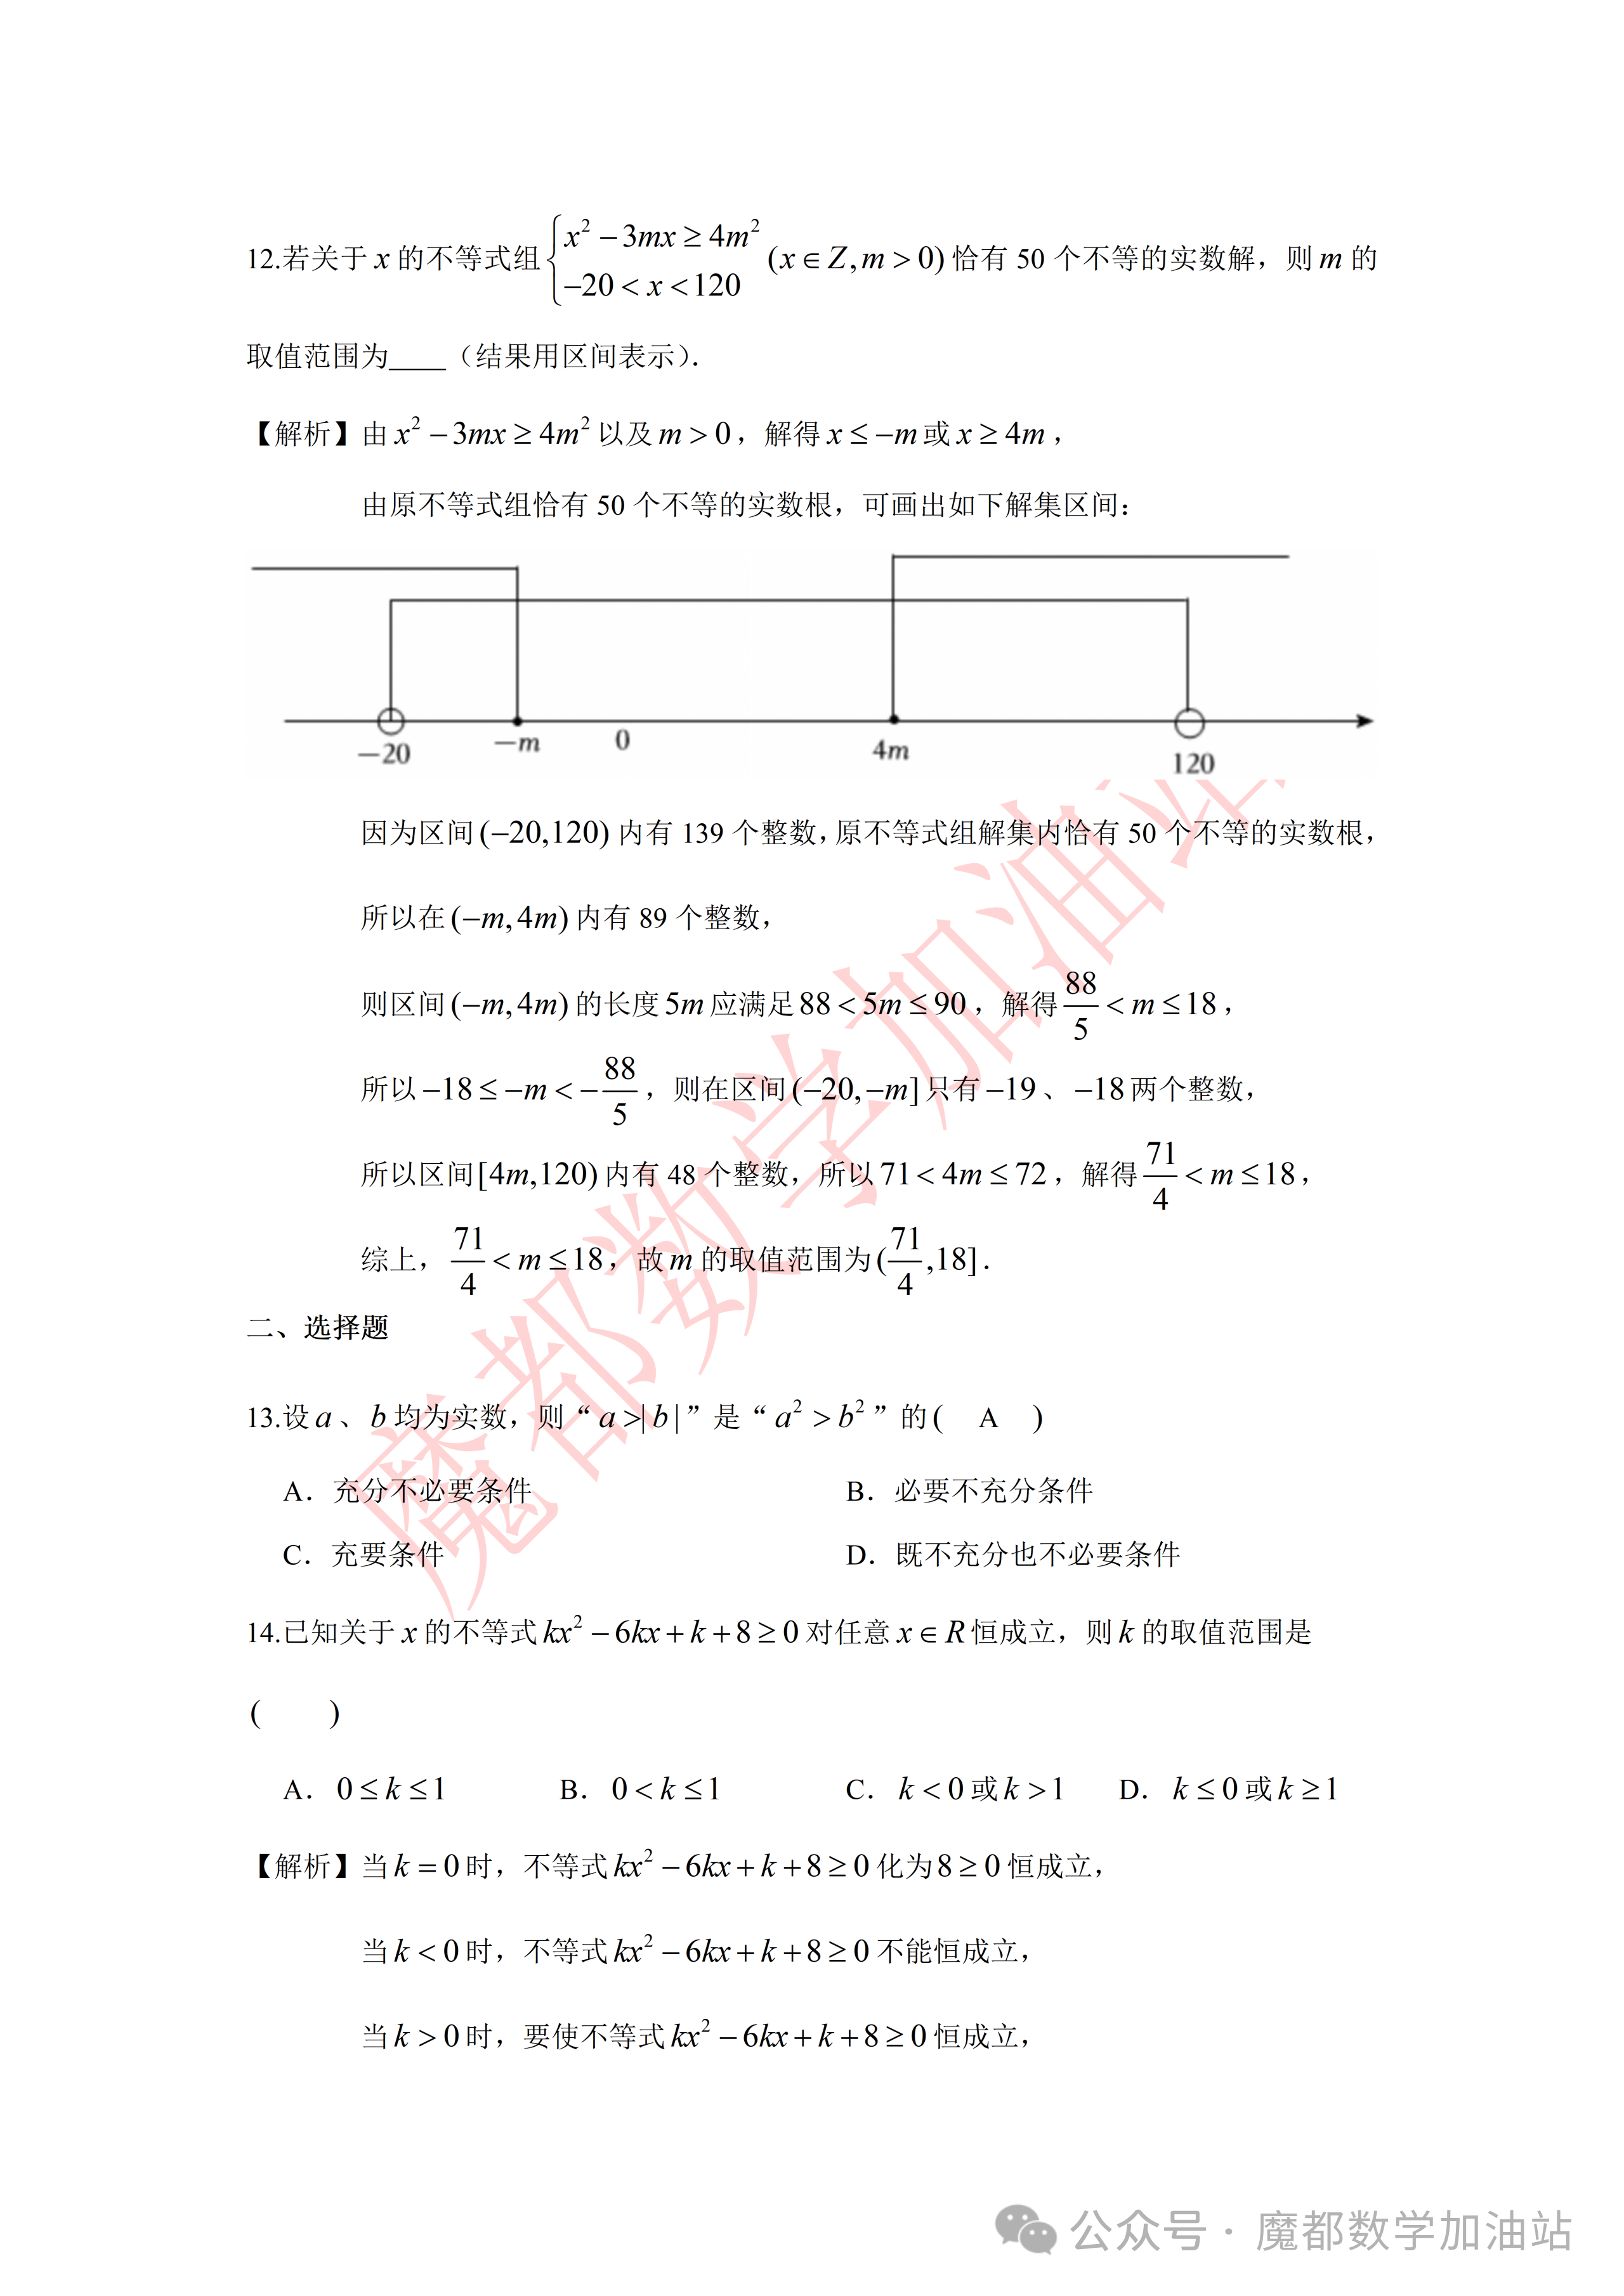
\includegraphics[width=.88\linewidth,trim=400bp 2410bp 320bp 860bp,clip]{../原图/高一46_交附闵行_国庆作业3/04.png}
\end{center}
\step{因为区间 $(-20,120)$ 内有 $139$ 个整数，原不等式组解集内有 $50$ 个不等的整数根，}
\step{所以在区间 $(-m,4m)$ 内有 $89$ 个整数，}
\step{则区间 $(-m,4m)$ 的长度 $5m$ 应满足 $88<5m\leqslant90$，解得 $\dfrac{88}{5}<m\leqslant18$，}
% 注：原卷题干称“实数解”，本行及后文按原卷解析照录为整数根计数。
\step{所以 $-18\leqslant-m<-\dfrac{88}{5}$，则在区间 $(-20,-m]$ 内有 $-19$、$-18$ 两个整数，}
\step{所以区间 $[4m,120)$ 内有 $48$ 个整数，}
\step{则 $71<4m\leqslant72$，解得 $\dfrac{71}{4}<m\leqslant18$，}
\step{综上，$\dfrac{71}{4}<m\leqslant18$，故 $m$ 的取值范围为 $\left(\dfrac{71}{4},18\right]$.}
\solend
\fi

\end{enumerate}

\bigsec{二、选择题}

\begin{enumerate}
\setcounter{enumi}{12}

\item 设 $a$、$b$ 均为实数，则“$a>|b|$”是“$a^2>b^2$”的\mbox{（\quad）}

\keepwithprev
A. 充分不必要条件\qquad B. 必要不充分条件

C. 充要条件\qquad\qquad D. 既不充分也不必要条件

\ans{$A$}

\item 已知关于 $x$ 的不等式 $kx^2-6kx+k+8\geqslant0$ 对任意 $x\in\R$ 恒成立，则 $k$ 的取值范围是\mbox{（\quad）}

\keepwithprev
A. $0\leqslant k\leqslant1$\qquad B. $0<k\leqslant1$

C. $k<0$ 或 $k>1$\qquad D. $k\leqslant0$ 或 $k\geqslant1$

\ans{$A$}

\ifanswer
\solbegin
\step{当 $k=0$ 时，不等式 $kx^2-6kx+k+8\geqslant0$ 化为 $8\geqslant0$ 恒成立，}
\step{当 $k<0$ 时，不等式 $kx^2-6kx+k+8\geqslant0$ 不能恒成立，}
\step{当 $k>0$ 时，要使不等式 $kx^2-6kx+k+8\geqslant0$ 恒成立，}
\step{需 $\Delta=36k^2-4(k^2+8k)\leqslant0$，解得 $0\leqslant k\leqslant1$，故选 $A$.}
\solend
\fi

\item 已知关于 $x$ 的不等式 $a\leqslant\dfrac34x^2-3x+4\leqslant b$，下列结论正确的是\mbox{（\quad）}

\keepwithprev
A. 当 $a<b<1$ 时，不等式 $a\leqslant\dfrac34x^2-3x+4\leqslant b$ 的解集非空

B. 当 $a=2$ 时，不等式 $a\leqslant\dfrac34x^2-3x+4\leqslant b$ 的解集可以为 $\{x\mid c\leqslant x\leqslant d\}$ 的形式

C. 不等式 $a\leqslant\dfrac34x^2-3x+4\leqslant b$ 的解集恰好为 $\{x\mid a\leqslant x\leqslant b\}$，那么 $b=\dfrac43$

D. 不等式 $a\leqslant\dfrac34x^2-3x+4\leqslant b$ 的解集恰好为 $\{x\mid a\leqslant x\leqslant b\}$，那么 $b-a=4$

\ans{$D$}

\ifanswer
\solbegin
\step{由 $\dfrac34x^2-3x+4\leqslant b$，得 $3x^2-12x+16-4b\leqslant0$，又 $b<1$，}
\step{所以 $\Delta=144-12(16-4b)=48(b-1)<0$，从而不等式无解，故 $A$ 错误；}
\step{在同一平面直角坐标系中作出函数 $y=\dfrac34x^2-3x+4=\dfrac34(x-2)^2+1$ 的图象及直线 $y=a$ 和 $y=b$，如图所示.}
\begin{center}
% 原图第 5 页解析配图直接裁取。
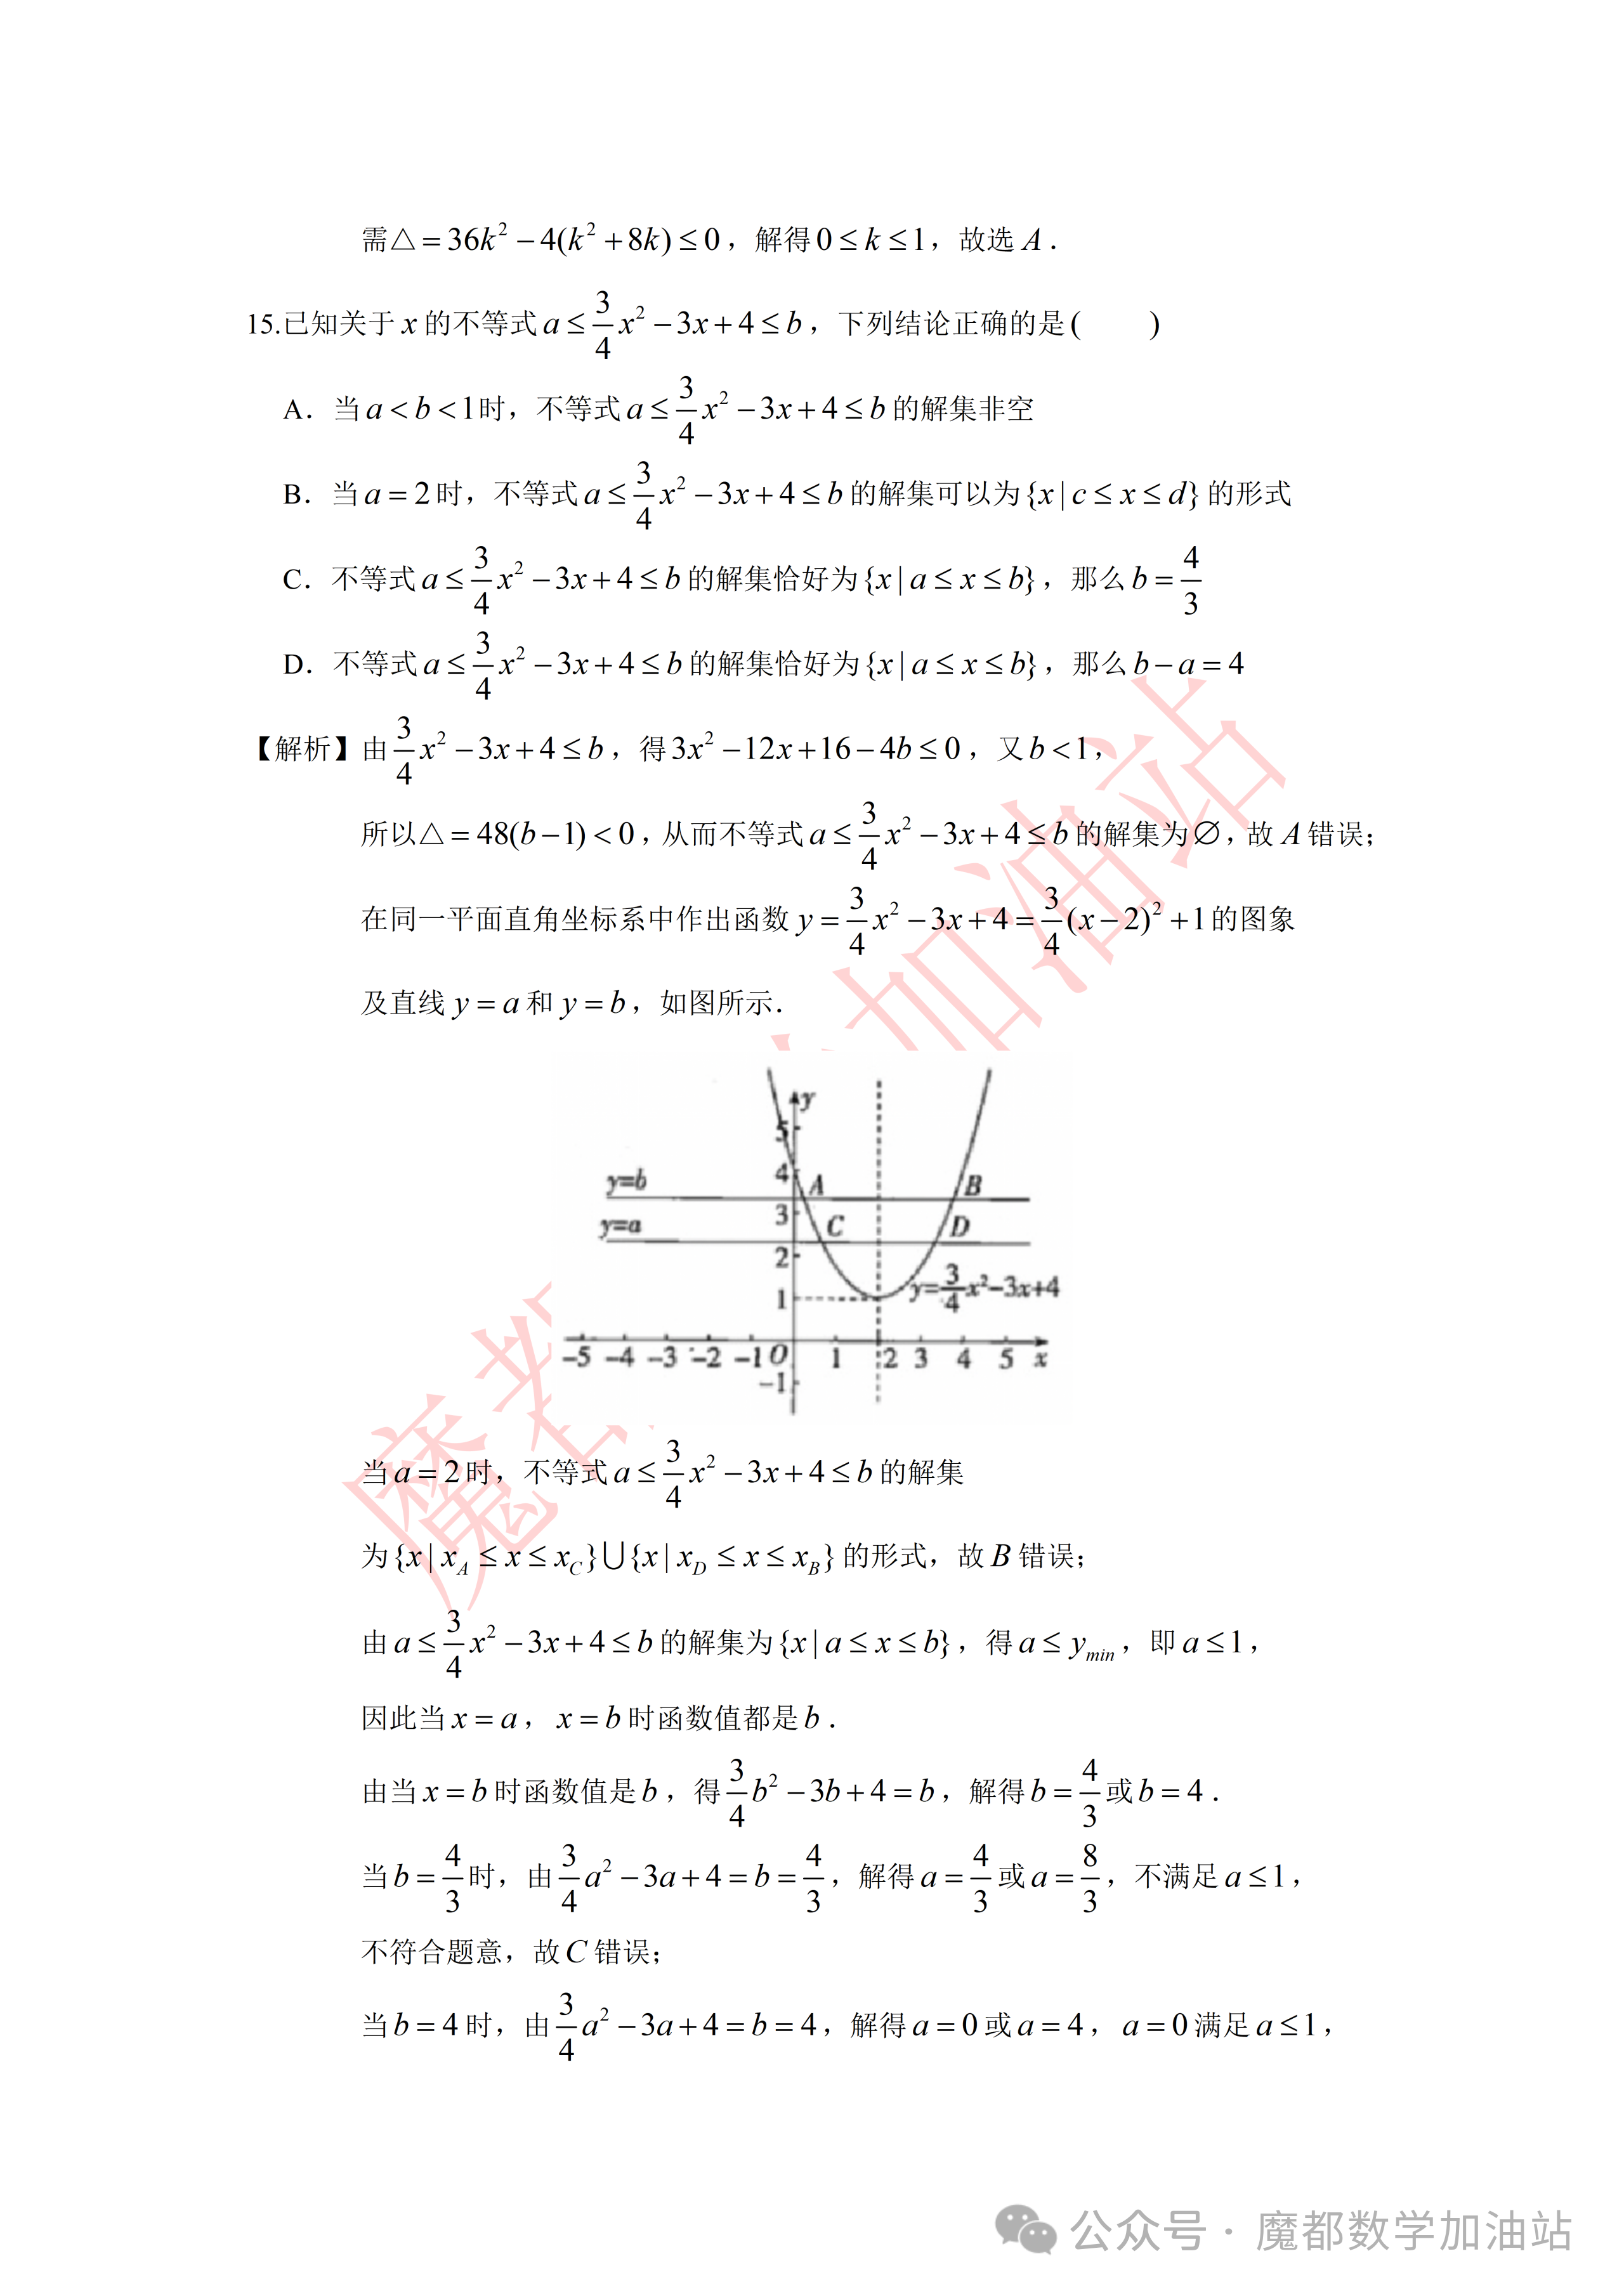
\includegraphics[width=.55\linewidth,trim=900bp 1400bp 760bp 1680bp,clip]{../原图/高一46_交附闵行_国庆作业3/05.png}
\end{center}
\step{当 $a=2$ 时，不等式 $a\leqslant\dfrac34x^2-3x+4\leqslant b$ 的解集为
$\{x\mid x_A\leqslant x\leqslant x_C\}\cup\{x\mid x_D\leqslant x\leqslant x_B\}$ 的形式，故 $B$ 错误；}
\step{由 $a\leqslant\dfrac34x^2-3x+4\leqslant b$ 的解集恰好为 $\{x\mid a\leqslant x\leqslant b\}$ 的形式，得 $a\leqslant y_{\min}$，即 $a\leqslant1$，}
\step{因为当 $x=a$、$x=b$ 时函数值都是 $b$，当 $x=a$ 时，$\dfrac34a^2-3a+4=b$；当 $x=b$ 时，$\dfrac34b^2-3b+4=b$，}
\step{解得 $b=\dfrac43$ 或 $b=4$，}
\step{当 $b=\dfrac43$ 时，由 $\dfrac34a^2-3a+4=b$，解得 $a=\dfrac43$ 或 $a=\dfrac83$，不符合题意，故 $C$ 错误；}
\step{当 $b=4$ 时，由 $\dfrac34a^2-3a+4=b$，解得 $a=0$ 或 $a=4$，$a=0$ 满足 $a\leqslant1$，故 $D$ 正确；}
\step{故选 $D$.}
\solend
\fi

\item 已知 $x$、$y\in(0,+\infty)$，则 $(x-y)^2+2y+1-x+\dfrac4x$ 的最小值为\mbox{（\quad）}

\keepwithprev
A. $1$\qquad B. $2$\qquad C. $3$\qquad D. $4$

\ans{$D$}

\ifanswer
\solbegin
\step{因为 $(x-y)^2+2y+1-x+\dfrac4x=(x-y-1)^2+x+\dfrac4x$，}
\step{当且仅当 $x-y-1=0$，且 $x=\dfrac4x$ 时取等号，}
\step{又因为 $x+\dfrac4x\geqslant2\sqrt{x\cdot\dfrac4x}=4$，当且仅当 $x=2$ 时取等号，}
\step{故选 $D$.}
\solend
\fi

\end{enumerate}

\bigsec{三、解答题}

\begin{enumerate}
\setcounter{enumi}{16}

\item 设集合 $A=\left\{x\middle|\dfrac{x-3}{x-1}<0\right\}$，$B=\{x\mid x^2-2ax+a^2-1>0\}$.
\begin{enumerate}[label=(\arabic*)]
\item 若 $a=3$，求 $A\cup B$；
\item 若“$x\in A$”是“$x\in B$”的充分条件，求实数 $a$ 的取值范围.
\end{enumerate}

\ifanswer
\solbegin
% 注：原卷题干为 a^2-1，故 a=3 时常数项为 8；题干与本步一致。
\stepm{(1)}{当 $a=3$ 时，$B=\{x\mid x^2-6x+8>0\}=\{x\mid x<2\text{ 或 }x>4\}$；}
\step{因为 $A=\left\{x\middle|\dfrac{x-3}{x-1}<0\right\}=\{x\mid(x-1)(x-3)<0\}=\{x\mid1<x<3\}$，}
\step{所以 $A\cup B=\{x\mid x<2\text{ 或 }x>4\}\cup\{x\mid1<x<3\}
=\{x\mid x<3\text{ 或 }x>4\}$.}
\stepm{(2)}{因为“$x\in A$”是“$x\in B$”的充分条件，所以 $A\subseteq B$，}
\step{因 $A=\left\{x\middle|\dfrac{x-3}{x-1}<0\right\}
=\{x\mid(x-1)(x-3)<0\}=\{x\mid1<x<3\}$，}
\step{所以 $A\subseteq B=\{x\mid x<a-1\text{ 或 }x>a+1\}$，}
\step{要使 $A\subseteq B$，需有 $a-1\geqslant3$ 或 $a+1\leqslant1$，}
\step{所以 $a\geqslant4$ 或 $a\leqslant0$，故 $a$ 的取值范围为 $\{a\mid a\geqslant4\text{ 或 }a\leqslant0\}$.}
\solend
\fi

\ansspace[6]

\item 某学校引入种植类劳动教育课程，打算围成如图所示的四块全等的长方形田地种植不同种类的蔬菜，其中一面可以利用原有的墙（足够长），其他各面需要用篱笆围成，设其中一块田地为矩形 $ABCD$.

\begin{center}
% 原图第 6 页配图直接裁取。
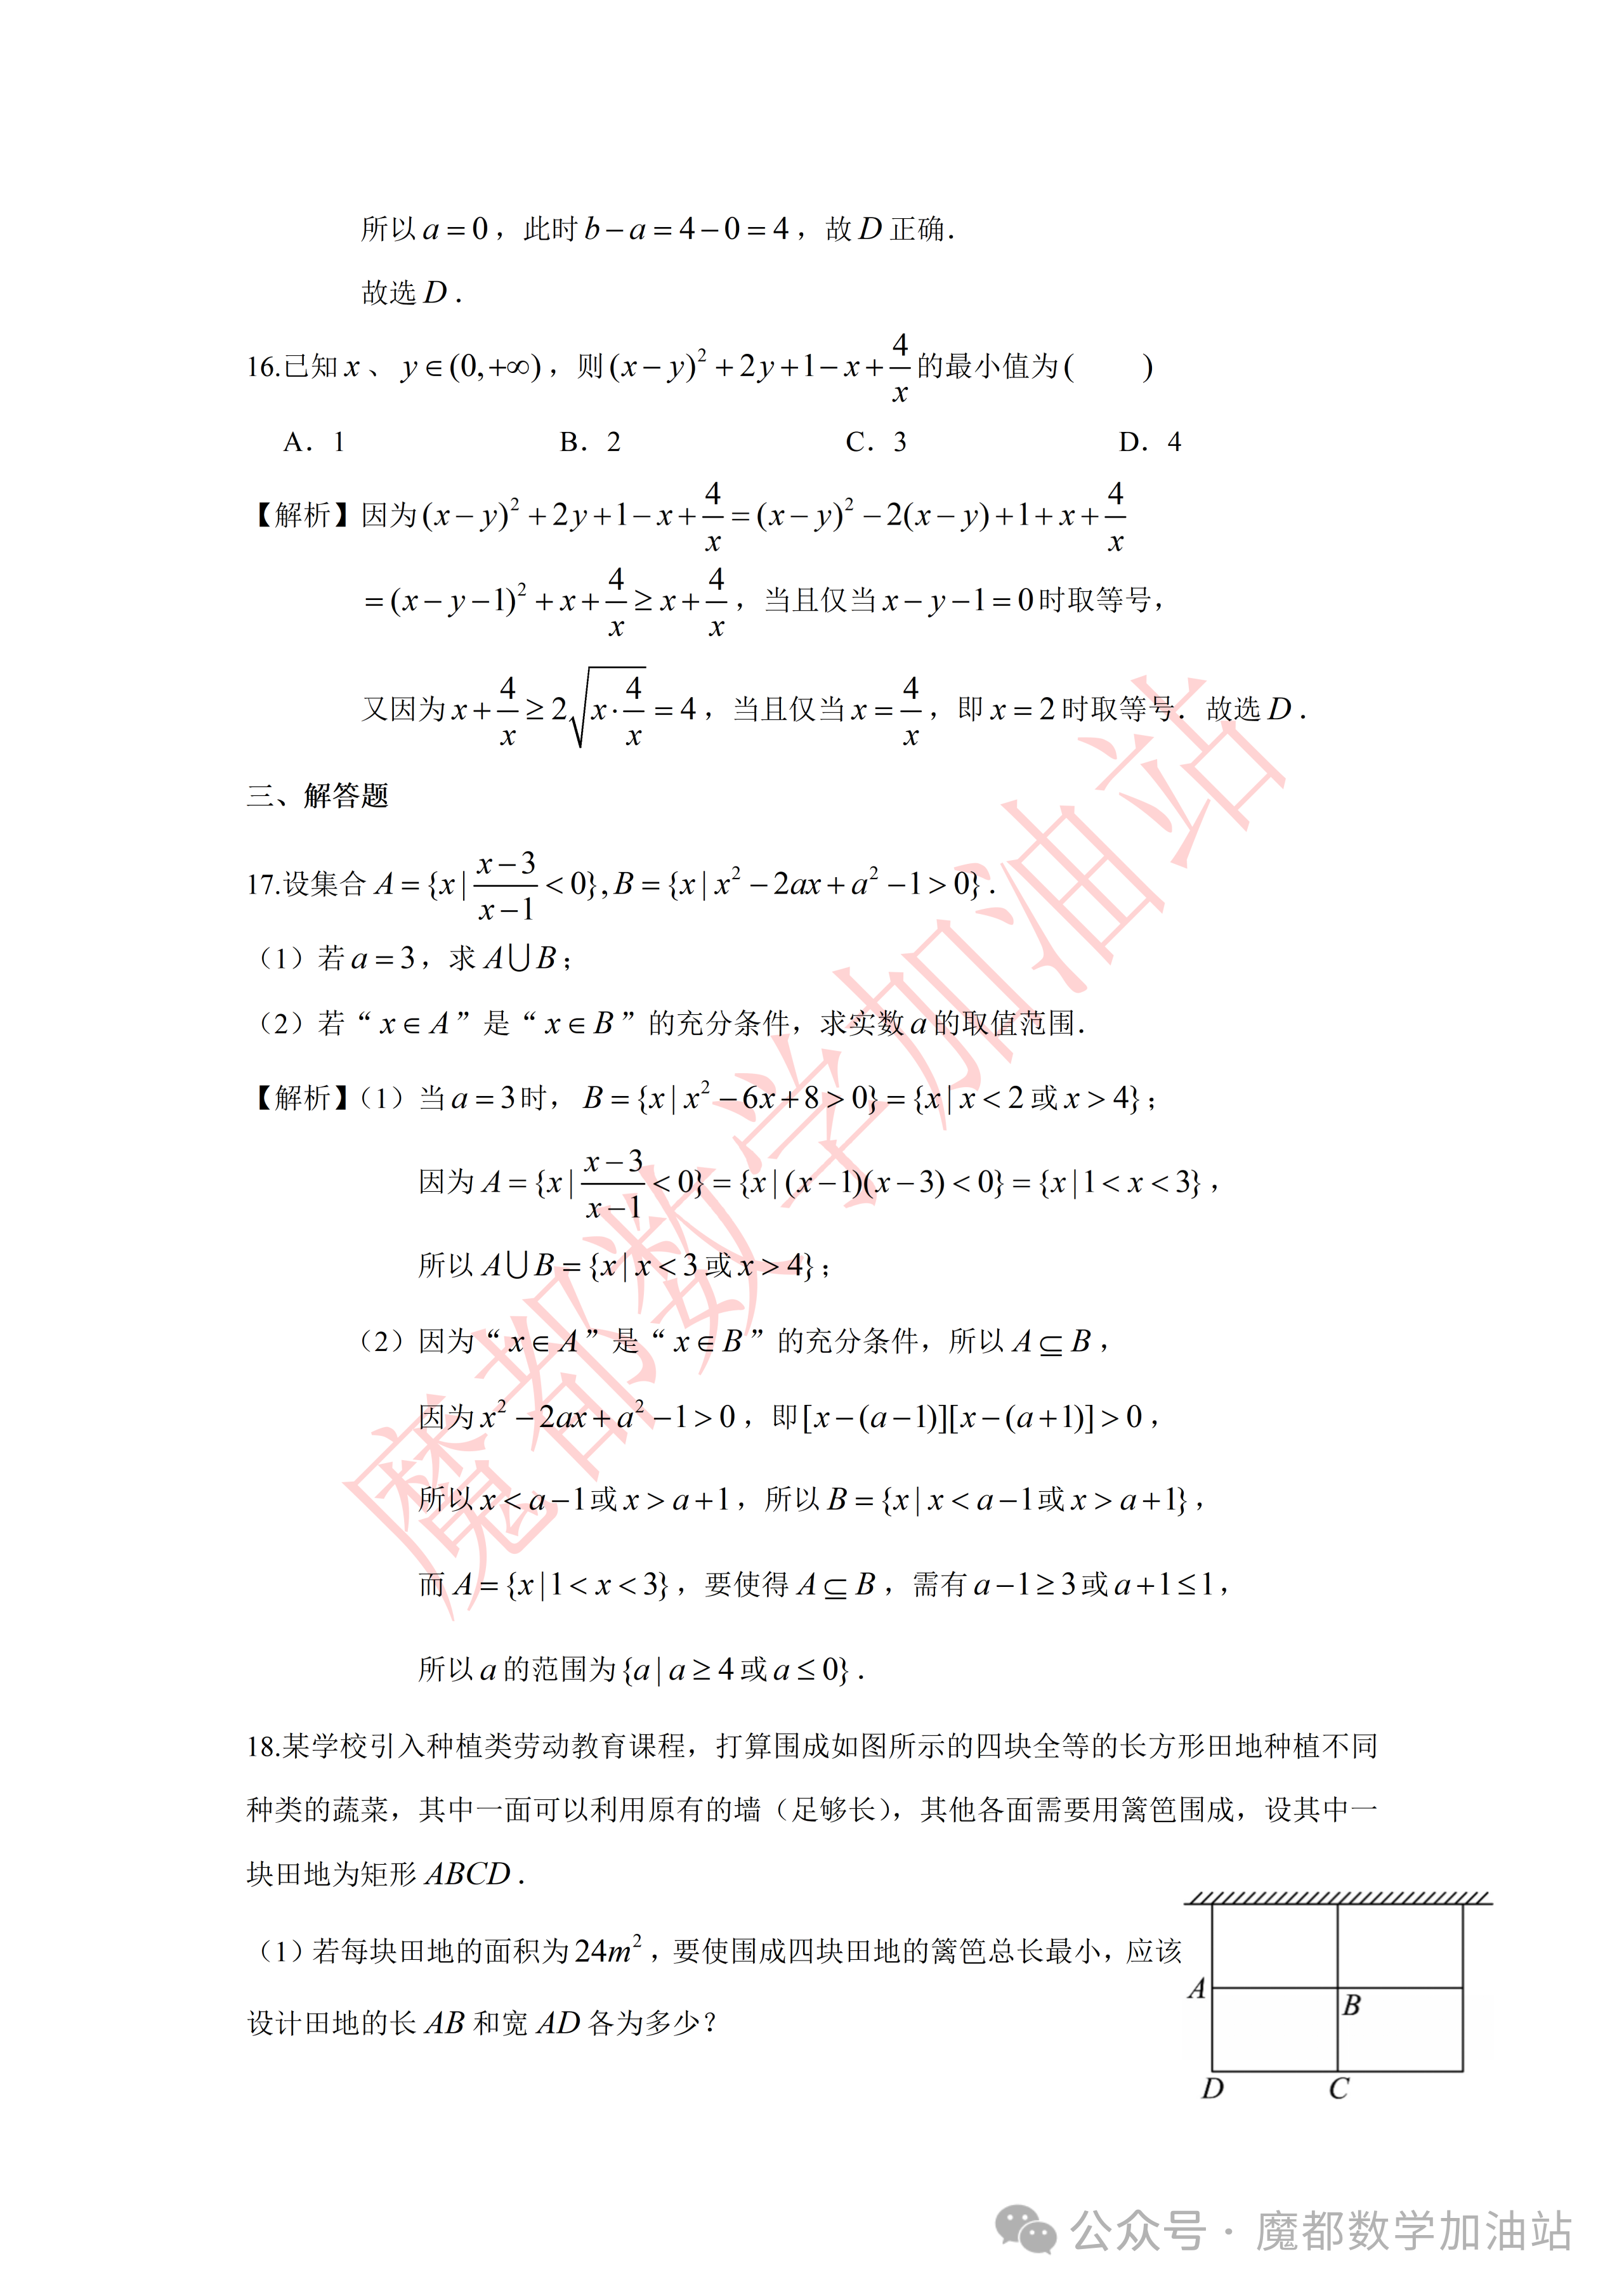
\includegraphics[width=.33\linewidth,trim=1866bp 220bp 210bp 2960bp,clip]{../原图/高一46_交附闵行_国庆作业3/06.png}
\end{center}

\begin{enumerate}[label=(\arabic*)]
\item 若每块田地的面积为 $24\,\text{m}^2$，要使围成四块田地的篱笆总长最小，应该设计田地的长 $AB$ 和宽 $AD$ 各为多少？
\item 现有 $40\,\text{m}$ 长的篱笆，要使每块田地的面积最大，应该设计田地的长 $AB$ 和宽 $AD$ 各为多少？
\end{enumerate}

\ifanswer
\solbegin
\stepm{(1)}{设 $AB$ 长为 $x\,\text{m}$，$AD$ 宽为 $y\,\text{m}$，由题意得 $xy=24$，篱笆总长为 $4x+6y$，}
\step{$4x+6y\geqslant2\sqrt{4x\cdot6y}=2\sqrt{24xy}=48$，}
\step{当且仅当 $4x=6y$ 时取等号，解得 $x=6$，$y=4$，}
\step{所以田地的长 $AB$ 为 $6\,\text{m}$，宽 $AD$ 为 $4\,\text{m}$.}
\stepm{(2)}{设 $AB$ 长为 $a\,\text{m}$，$AD$ 宽为 $b\,\text{m}$，由篱笆总长 $4a+6b=40$，即 $2a+3b=20$，}
\step{将 $a=\dfrac{20-3b}{2}$ 代入每块田地面积 $ab$，得 $ab=\dfrac12b(20-3b)=-\dfrac32b^2+10b$，}
\step{当 $b=\dfrac{10}{3}$ 时，$ab$ 最大，此时 $a=5$，}
\step{所以田地的长 $AB$ 为 $5\,\text{m}$，宽 $AD$ 为 $\dfrac{10}{3}\,\text{m}$.}
\solend
\fi

\ansspace[8]

\item 已知 $x_1$、$x_2$ 是一元二次方程 $4kx^2-4kx+k+1=0$ 的两个不等实数根.
\begin{enumerate}[label=(\arabic*)]
\item 若 $x_1$、$x_2$ 均为正根，求实数 $k$ 的取值范围；
\item 求使 $\dfrac{x_1}{x_2}+\dfrac{x_2}{x_1}-2$ 的值为整数 $k$ 的整数值.
\end{enumerate}

\ifanswer
\solbegin
\stepm{(1)}{由题意，$x_1$、$x_2$ 是方程 $4kx^2-4kx+k+1=0$ 的两个不等实数根，}
\step{故 $k\neq0$，$\Delta=(-4k)^2-16k(k+1)>0$，得 $-16k>0$，所以 $k<0$，}
\step{又 $x_1+x_2=1$，$x_1x_2=\dfrac{k+1}{4k}>0$，得 $k+1<0$，}
\step{所以 $k$ 的取值范围为 $(-\infty,-1)$.}
\stepm{(2)}{由题意，}
\step{$\dfrac{x_1}{x_2}+\dfrac{x_2}{x_1}-2
=\dfrac{x_1^2+x_2^2-2x_1x_2}{x_1x_2}
=\dfrac{(x_1+x_2)^2-4x_1x_2}{x_1x_2}$，}
\step{又 $x_1+x_2=1$，$x_1x_2=\dfrac{k+1}{4k}$，}
\step{则 $\dfrac{x_1}{x_2}+\dfrac{x_2}{x_1}-2=-\dfrac4{k+1}$，}
\step{由于 $-\dfrac4{k+1}$ 为整数，故 $k+1$ 只能取 $\pm1$、$\pm2$、$\pm4$，又 $k<-1$，}
\step{所以整数 $k$ 的值为 $-2$、$-3$、$-5$.}
\solend
\fi

\ansspace[8]

\item 已知 $a>0$，$b>0$，且 $2a+3b=3$.
\begin{enumerate}[label=(\arabic*)]
\item 求 $ab$ 的最大值；
\item 求 $a-\dfrac1{6b}$ 的最大值；
\item 求 $\dfrac2a+\dfrac3{b+1}$ 的最小值.
\end{enumerate}

\ifanswer
\solbegin
\stepm{(1)}{由 $2a+3b=3$，得 $3=2a+3b\geqslant2\sqrt{6ab}$，}
\step{所以 $ab\leqslant\dfrac38$，当且仅当 $2a=3b=\dfrac32$ 时取等号，}
\step{故 $ab$ 的最大值为 $\dfrac38$.}
\stepm{(2)}{由 $2a+3b=3$，得 $a=\dfrac32-\dfrac32b$，}
\step{则 $a-\dfrac1{6b}=\dfrac32-\dfrac32b-\dfrac1{6b}$，}
\step{由基本不等式，$\dfrac32b+\dfrac1{6b}\geqslant2\sqrt{\dfrac32b\cdot\dfrac1{6b}}=1$，}
\step{当且仅当 $\dfrac32b=\dfrac1{6b}$，即 $b=\dfrac13$、$a=1$ 时取等号，}
\step{所以 $a-\dfrac1{6b}$ 的最大值为 $\dfrac12$.}
\stepm{(3)}{由 $2a+3b=3$，得 $2a+3(b+1)=6$，}
\step{$\dfrac2a+\dfrac3{b+1}
=\dfrac16\left(2a+3(b+1)\right)\left(\dfrac2a+\dfrac3{b+1}\right)$}
\step{$=\dfrac16\left(13+\dfrac{6(b+1)}a+\dfrac{6a}{b+1}\right)
\geqslant\dfrac16\left(13+2\sqrt{\dfrac{6(b+1)}a\cdot\dfrac{6a}{b+1}}\right)=\dfrac{25}{6}$，}
\step{当且仅当 $a=b+1$，即 $a=\dfrac65$、$b=\dfrac15$ 时取等号，}
\step{所以 $\dfrac2a+\dfrac3{b+1}$ 的最小值为 $\dfrac{25}{6}$.}
\solend
\fi

\ansspace[8]

\item 已知 $U=\R$ 为全集，集合 $A=\{s^2+3t^2\mid s,t\in U\}$.
\begin{enumerate}[label=(\arabic*)]
\item 设 $U=\{1,3,5\}$，求集合 $A$ 的元素个数；
\item 设 $U=\Z$，证明：若 $x\in A$，则 $7x\in A$；
\item 设 $U=\R$，$x$、$y\in A$，且 $x=m^2+3n^2$，$y=p^2+3q^2$，若 $mp-3nq=\sqrt3$，求 $x+y+mq+np$ 的最小值.
\end{enumerate}

\ifanswer
\solbegin
\stepm{(1)}{当 $s=1$，$t=1$ 时，$s^2+3t^2=1+3=4$；}
\step{当 $s=1$，$t=3$ 时，$s^2+3t^2=1+27=28$；}
\step{当 $s=1$，$t=5$ 时，$s^2+3t^2=1+75=76$；}
\step{当 $s=3$，$t=1$ 时，$s^2+3t^2=9+3=12$；}
\step{当 $s=3$，$t=3$ 时，$s^2+3t^2=9+27=36$；}
\step{当 $s=3$，$t=5$ 时，$s^2+3t^2=9+75=84$；}
\step{当 $s=5$，$t=1$ 时，$s^2+3t^2=25+3=28$；}
\step{当 $s=5$，$t=3$ 时，$s^2+3t^2=25+27=52$；}
\step{当 $s=5$，$t=5$ 时，$s^2+3t^2=25+75=100$，}
\step{所以 $A=\{4,12,28,36,52,76,84,100\}$，有 $8$ 个元素.}
\stepm{(2)}{因为 $U=\Z$，$x\in A$，设 $x=s^2+3t^2$，}
\step{则 $7x=7(s^2+3t^2)=(2s+3t)^2+3(s-2t)^2\in A$，}
\step{所以 $7x\in A$.}
\stepm{(3)}{因为 $x=m^2+3n^2$，$y=p^2+3q^2$，}
\step{$xy=(m^2+3n^2)(p^2+3q^2)=3(mq+np)^2+(mp-3nq)^2$，}
\step{设 $mq+np=b$，则 $xy=3b^2+3$，所以 $y=\dfrac{3b^2+3}{x}$，}
\step{于是 $x+y+mq+np=x+\dfrac{3b^2+3}{x}+b\geqslant2\sqrt{3b^2+3}+b$，}
\step{设 $2\sqrt{3b^2+3}+b=t$，整理得 $11b^2+2bt+12-t^2=0$，}
\step{判别式法，$\Delta=4t^2-44(12-t^2)\geqslant0$，得 $t\geqslant\sqrt{11}$，}
\step{即 $(x+y+mq+np)_{\min}=\sqrt{11}$，所以 $x+y+mq+np$ 的最小值为 $\sqrt{11}$.}
\solend
\fi

\ansspace*[10]

\end{enumerate}

\end{document}
"
% 紧凑版：xelatex "\def\iscompact{1}% 高一46_交附闵行_国庆作业3.tex
%   —— 高一上数学“2026-2027 年交附闵行高一上国庆作业 3”（讲评版）
% 试卷版：xelatex 高一46_交附闵行_国庆作业3.tex
% 答案版：xelatex "\def\isanswer{1}\input{高一46_交附闵行_国庆作业3.tex}"
% 紧凑版：xelatex "\def\iscompact{1}\input{高一46_交附闵行_国庆作业3.tex}"
%
% 原始材料：微信公众号“魔都数学加油站”，作者破晓，2026-10-02 17:56 发布。
% 原文标题：“27学年高一46——2026-2027你那上海市交附闵行高一上国庆作业3”
% （公众号标题中的“你那”照录，系原文标题字样）；原文链接：
% http://mp.weixin.qq.com/s?__biz=Mzg4ODU1ODMxOQ==&mid=2247591657&idx=3&sn=a894d1a16611283a61b3eaba32a3f24c&chksm=cee83366c6a55381b370069f84ef63d20251f94608bb37cc4ec2d66227401bd147f4f6bd8256&scene=126&sessionid=1790935402&subscene=7&clicktime=1790937618&enterid=1790937618#rd
% 正文为 9 张 PNG 页，按页序读取原图；第 01、02、07 页 4762×6735，
% 第 03—06、08、09 页 2560×3620。卷面标题照原卷印作“2026-2027 年交附闵行高一上国庆作业 3”。
% 原文从第 3 题起，题号照原卷保留；正文为讲评版，答案、解析依原卷顺序录入。
% 水印及页脚公众号标识不录入。卷面插图直接裁取对应原图页，不另制图片文件。
%
% 与原卷的排版差异：
%   ① 原卷按“一、填空题”“二、选择题”“三、解答题”分节，本稿沿用原节与原题号，
%      只改排为全稿统一的大节样式；
%   ② 原卷答案与解析依页面位置分布，本稿按 common.sty 统一置于答案版；
%   ③ 原卷副标题未印，本稿按“知识模块”口径标作“集合与常用逻辑用语、不等式”。
%
% 原卷存疑一处（照抄未改，见第 12 题题干及解析处注释）：
%   第 12 题题干同时给出 x∈Z，却称不等式组有“50 个不等的实数解”；解析按整数根计数。
%   此处题干与解析的原文不一致，本稿均照录。
% 第 17 题曾疑似有常数项不一致：复核原图题干为 a^2-1，a=3 时常数项确为 8，
% 与解析相符；不将其记作原卷错误。
%
\documentclass[a4paper,11pt]{article}
\usepackage{common}

\begin{document}

\examtitlest[3]{2026--2027 年交附闵行高一上国庆作业 3}{集合与常用逻辑用语、不等式}

\bigsec{一、填空题}

\begin{enumerate}
\setcounter{enumi}{2}

\item 不等式 $\dfrac{x^2-10}{x+2}\geqslant1$ 的解集为\blankline[4.4em].

\ifanswer
\ans{$\{x\mid-3\leqslant x<-2\text{ 或 }x\geqslant4\}$}
\solbegin
\step{不等式 $\dfrac{x^2-10}{x+2}\geqslant1$，移项得 $\dfrac{x^2-10}{x+2}-1\geqslant0$，}
\step{通分得 $\dfrac{x^2-x-12}{x+2}\geqslant0$，即 $\dfrac{(x-4)(x+3)}{x+2}\geqslant0$，}
\step{解得 $-3\leqslant x<-2$ 或 $x\geqslant4$，}
\step{故不等式的解集为 $\{x\mid-3\leqslant x<-2\text{ 或 }x\geqslant4\}$.}
\solend
\fi

\item $|x-3|+|x-5|\geqslant2$，当等号成立时，$x$ 的范围是\blankline[4.4em].

\ifanswer
\ans{$[3,5]$}
\fi

\item 若直角三角形斜边长等于 $4\sqrt2\,\text{cm}$，则直角三角形面积的最大值为\blankline[4.4em].

\ifanswer
\solbegin
\step{设 $Rt\triangle ABC$ 中，$C=90^\circ$，则 $c=\sqrt{a^2+b^2}=4\sqrt2$，所以 $a^2+b^2=32$，}
\step{由基本不等式得 $a^2+b^2\geqslant2ab$，当且仅当 $a=b=4$ 时取等号，}
\step{所以 $\triangle ABC$ 的面积 $S=\dfrac12ab\leqslant8$，}
\step{当且仅当 $a=b=4$ 时，$\triangle ABC$ 的面积最大值为 $8$.}
\solend
\fi

\item 不等式 $(x-1)(2-x)>0$ 的解集为\blankline[4.4em].

\ifanswer
\solbegin
\step{$(x-1)(2-x)>0\Rightarrow(x-1)(x-2)<0$，}
\step{故不等式的解集为 $\{x\mid1<x<2\}$.}
\solend
\fi

\item 已知集合 $A=\{1,2\}$，$B=\{x\mid x^2-2mx+m=0\}$，$A\cup B=A$，则实数 $m$ 的取值范围为\blankline[4.4em].

\ifanswer
\solbegin
\step{因为 $A\cup B=A$，所以 $B\subseteq A$，}
\step{当 $B=\varnothing$ 时，$\Delta=(-2m)^2-4m<0$，解得 $0<m<1$，}
\step{当 $B$ 为单元素集时，$\Delta=0$，解得 $m=0$ 或 $m=1$，}
\step{当 $m=0$ 时，方程 $x^2=0$，解得 $x=0$，此时 $B=\{0\}$，不满足 $B\subseteq A$；}
\step{当 $m=1$ 时，方程 $x^2-2x+1=0$，解得 $x=1$，此时 $B=\{1\}$，满足 $B\subseteq A$；}
\step{当 $B=\{1,2\}$ 时，由韦达定理得 $1+2=2m$，$1\times2=m$，无解，}
\step{综上所述，实数 $m$ 的取值范围为 $\{m\mid0<m\leqslant1\}$.}
\solend
\fi

\item 设 $a$、$b$、$c\in\R^+$，若 $a+b+c=1$，则 $\dfrac1a+\dfrac1b+\dfrac1c\geqslant$\blankline[4.4em].

\ifanswer
\solbegin
\step{因为 $a$、$b$、$c\in\R^+$，且 $a+b+c=1$，}
\step{所以 $\dfrac1a+\dfrac1b+\dfrac1c=(a+b+c)\left(\dfrac1a+\dfrac1b+\dfrac1c\right)$}
\step{$=3+\dfrac ab+\dfrac ba+\dfrac ac+\dfrac ca+\dfrac bc+\dfrac cb$，}
\step{由基本不等式得 $\dfrac ab+\dfrac ba\geqslant2$，$\dfrac ac+\dfrac ca\geqslant2$，$\dfrac bc+\dfrac cb\geqslant2$，}
\step{所以 $\dfrac1a+\dfrac1b+\dfrac1c\geqslant9$，当且仅当 $a=b=c=\dfrac13$ 时取等号，}
\step{所以 $\dfrac1a+\dfrac1b+\dfrac1c$ 的最小值为 $9$.}
\solend
\fi

\item 已知 $-1\leqslant x+y\leqslant2$，$-2\leqslant x-y\leqslant1$，则 $x-2y$ 的范围为\blankline[4.4em].

\ifanswer
\solbegin
\step{设 $x-2y=m(x+y)+n(x-y)$，}
\step{则 $x-2y=(m+n)x+(m-n)y$，所以 $m+n=1$，$m-n=-2$，}
\step{解得 $m=-\dfrac12$，$n=\dfrac32$，}
\step{所以 $x-2y=-\dfrac12(x+y)+\dfrac32(x-y)$，}
\step{因为 $-1\leqslant x+y\leqslant2$，$-2\leqslant x-y\leqslant1$，}
\step{所以 $-4\leqslant x-2y\leqslant2$，即 $x-2y$ 的范围为 $[-4,2]$.}
\solend
\fi

\item 设集合 $A=\{1,2,m\}$，其中 $m$ 为实数，令 $B=\{a^2\mid a\in A\}$，$C=A\cup B$. 若 $C$ 中所有元素之和为 $6$，则 $C$ 中的所有元素之积为\blankline[4.4em].

\ifanswer
\solbegin
\step{因为 $A=\{1,2,m\}$，所以 $B=\{a^2\mid a\in A\}=\{1,4,m^2\}$，$m\neq1$，$m\neq2$，}
\step{又 $C=A\cup B$，所以 $1\in C$，$4\in C$，$m^2\in C$，}
\step{若 $m^2=1$，则 $m=-1$ 或 $m=1$（舍），当 $m=-1$ 时，$C=\{1,2,4,-1\}$，$C$ 中所有元素之和为 $6$，}
\step{此时 $C$ 中所有元素之积为 $-8$；}
\step{若 $m^2=2$，则 $m=-\sqrt2$ 或 $m=\sqrt2$，$C$ 中所有元素之和不符合题意；}
\step{若 $m^2=4$，则 $m=-2$ 或 $m=2$，此时 $C=\{1,2,4,-2\}$ 或 $C=\{1,2,4\}$，所有元素之和不符合题意；}
\step{若 $m^2\neq1$，$m^2\neq2$，$m^2\neq4$，则 $C=\{1,2,4,m,m^2\}$，}
\step{所以 $1+2+4+m+m^2=6$，即 $m^2+m+1=0$，无解，}
\step{综上所述，$C$ 中所有元素之积为 $-8$.}
\solend
\fi

\item 若对任意实数 $x>0$，$y>0$，不等式 $x+\sqrt{xy}\leqslant a(x+y)$ 恒成立，则实数 $a$ 的最小值为\blankline[4.4em].

\ifanswer
\solbegin
\step{由不等式 $x+\sqrt{xy}\leqslant a(x+y)$ 对任意实数 $x>0$，$y>0$ 恒成立，}
\step{得 $a\geqslant\dfrac{x+\sqrt{xy}}{x+y}$，}
\step{设 $\sqrt{\dfrac yx}=t>0$，则 $a\geqslant\dfrac{1+t}{1+t^2}$，}
\step{$\dfrac{1+t}{1+t^2}\leqslant\dfrac{\sqrt2+1}{2}$，当且仅当 $t=\sqrt2-1$ 时取等号，}
\step{所以实数 $a$ 的最小值为 $\dfrac{\sqrt2+1}{2}$.}
\solend
\fi

% 注：原卷题干给出 x∈Z，却写“实数解”；解析按整数解计数，题干与解析不一致，照录未改。
\item 若关于 $x$ 的不等式组
$\begin{cases}x^2-3mx\geqslant4m^2\\-20<x<120\end{cases}$（$x\in\Z,m>0$）恰有 $50$ 个不等的实数解，则 $m$ 的取值范围为\blankline[4.4em]（结果用区间表示）.

\ifanswer
\solbegin
\step{由 $x^2-3mx\geqslant4m^2$ 以及 $m>0$，解得 $x\leqslant-m$ 或 $x\geqslant4m$，}
\step{由原不等式组恰有 $50$ 个不等的实数解，可画出如下解集区间：}
\begin{center}
% 原图第 4 页数轴图直接裁取。
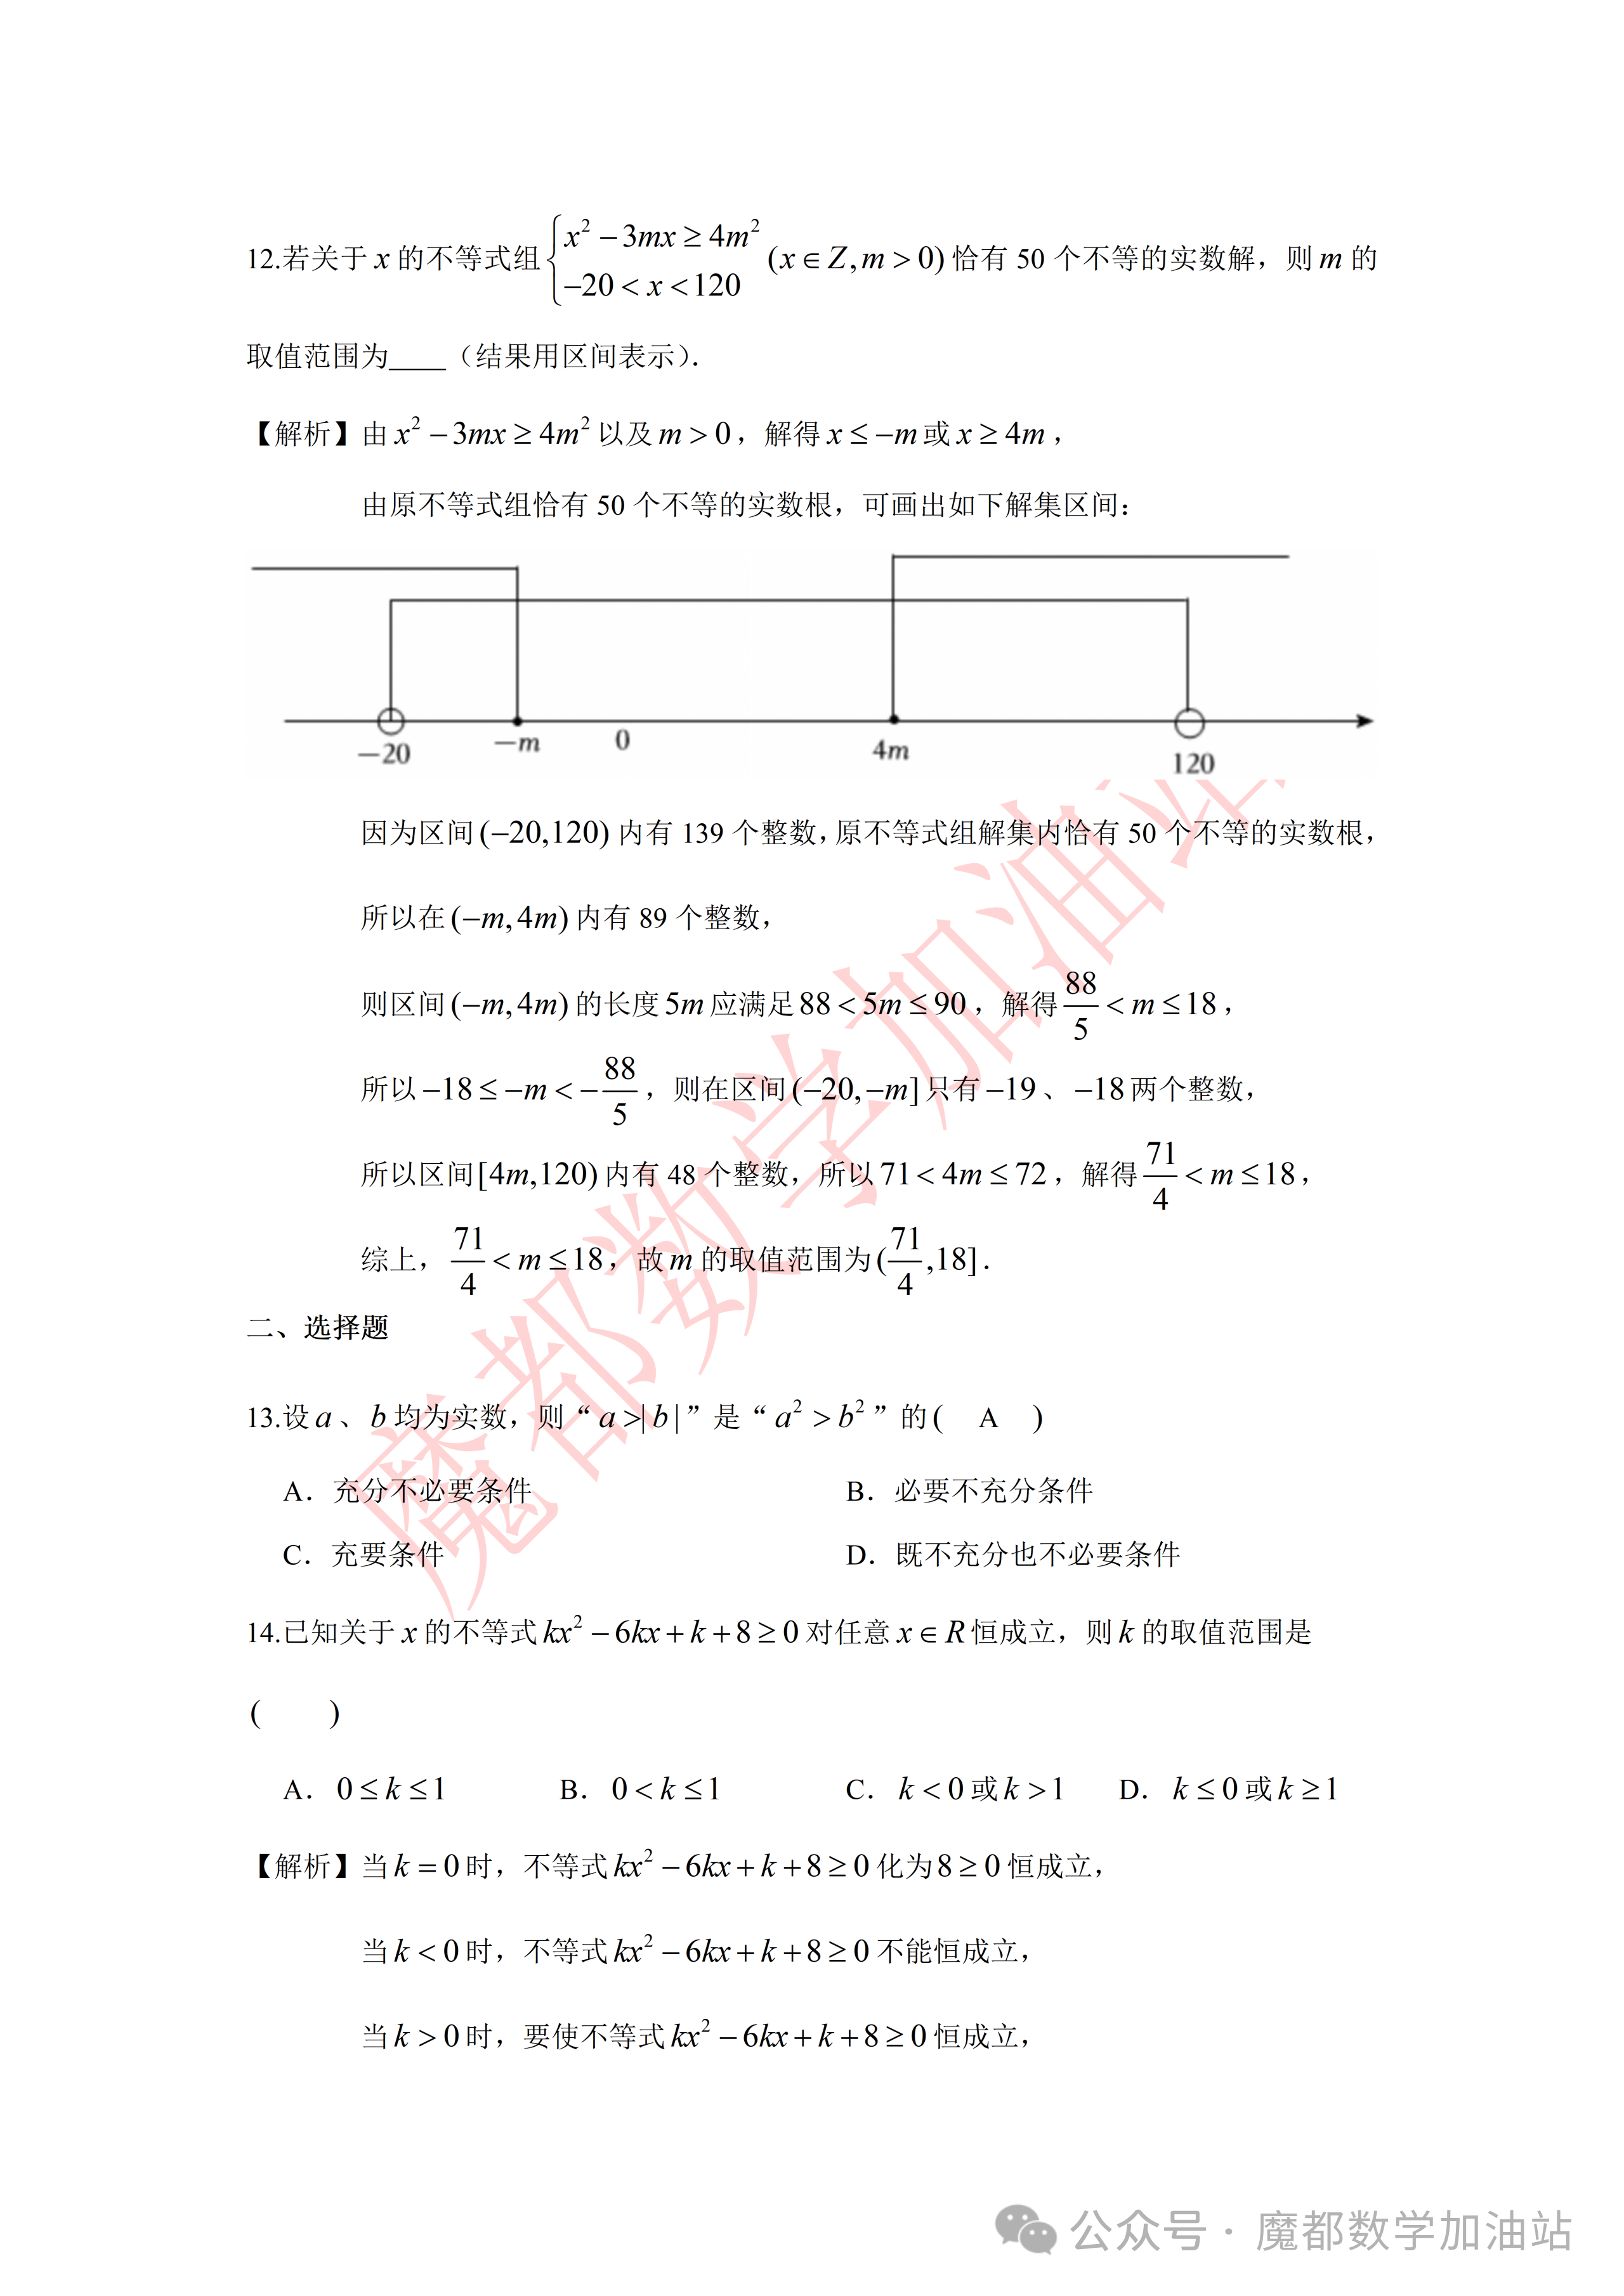
\includegraphics[width=.88\linewidth,trim=400bp 2410bp 320bp 860bp,clip]{../原图/高一46_交附闵行_国庆作业3/04.png}
\end{center}
\step{因为区间 $(-20,120)$ 内有 $139$ 个整数，原不等式组解集内有 $50$ 个不等的整数根，}
\step{所以在区间 $(-m,4m)$ 内有 $89$ 个整数，}
\step{则区间 $(-m,4m)$ 的长度 $5m$ 应满足 $88<5m\leqslant90$，解得 $\dfrac{88}{5}<m\leqslant18$，}
% 注：原卷题干称“实数解”，本行及后文按原卷解析照录为整数根计数。
\step{所以 $-18\leqslant-m<-\dfrac{88}{5}$，则在区间 $(-20,-m]$ 内有 $-19$、$-18$ 两个整数，}
\step{所以区间 $[4m,120)$ 内有 $48$ 个整数，}
\step{则 $71<4m\leqslant72$，解得 $\dfrac{71}{4}<m\leqslant18$，}
\step{综上，$\dfrac{71}{4}<m\leqslant18$，故 $m$ 的取值范围为 $\left(\dfrac{71}{4},18\right]$.}
\solend
\fi

\end{enumerate}

\bigsec{二、选择题}

\begin{enumerate}
\setcounter{enumi}{12}

\item 设 $a$、$b$ 均为实数，则“$a>|b|$”是“$a^2>b^2$”的\mbox{（\quad）}

\keepwithprev
A. 充分不必要条件\qquad B. 必要不充分条件

C. 充要条件\qquad\qquad D. 既不充分也不必要条件

\ans{$A$}

\item 已知关于 $x$ 的不等式 $kx^2-6kx+k+8\geqslant0$ 对任意 $x\in\R$ 恒成立，则 $k$ 的取值范围是\mbox{（\quad）}

\keepwithprev
A. $0\leqslant k\leqslant1$\qquad B. $0<k\leqslant1$

C. $k<0$ 或 $k>1$\qquad D. $k\leqslant0$ 或 $k\geqslant1$

\ans{$A$}

\ifanswer
\solbegin
\step{当 $k=0$ 时，不等式 $kx^2-6kx+k+8\geqslant0$ 化为 $8\geqslant0$ 恒成立，}
\step{当 $k<0$ 时，不等式 $kx^2-6kx+k+8\geqslant0$ 不能恒成立，}
\step{当 $k>0$ 时，要使不等式 $kx^2-6kx+k+8\geqslant0$ 恒成立，}
\step{需 $\Delta=36k^2-4(k^2+8k)\leqslant0$，解得 $0\leqslant k\leqslant1$，故选 $A$.}
\solend
\fi

\item 已知关于 $x$ 的不等式 $a\leqslant\dfrac34x^2-3x+4\leqslant b$，下列结论正确的是\mbox{（\quad）}

\keepwithprev
A. 当 $a<b<1$ 时，不等式 $a\leqslant\dfrac34x^2-3x+4\leqslant b$ 的解集非空

B. 当 $a=2$ 时，不等式 $a\leqslant\dfrac34x^2-3x+4\leqslant b$ 的解集可以为 $\{x\mid c\leqslant x\leqslant d\}$ 的形式

C. 不等式 $a\leqslant\dfrac34x^2-3x+4\leqslant b$ 的解集恰好为 $\{x\mid a\leqslant x\leqslant b\}$，那么 $b=\dfrac43$

D. 不等式 $a\leqslant\dfrac34x^2-3x+4\leqslant b$ 的解集恰好为 $\{x\mid a\leqslant x\leqslant b\}$，那么 $b-a=4$

\ans{$D$}

\ifanswer
\solbegin
\step{由 $\dfrac34x^2-3x+4\leqslant b$，得 $3x^2-12x+16-4b\leqslant0$，又 $b<1$，}
\step{所以 $\Delta=144-12(16-4b)=48(b-1)<0$，从而不等式无解，故 $A$ 错误；}
\step{在同一平面直角坐标系中作出函数 $y=\dfrac34x^2-3x+4=\dfrac34(x-2)^2+1$ 的图象及直线 $y=a$ 和 $y=b$，如图所示.}
\begin{center}
% 原图第 5 页解析配图直接裁取。
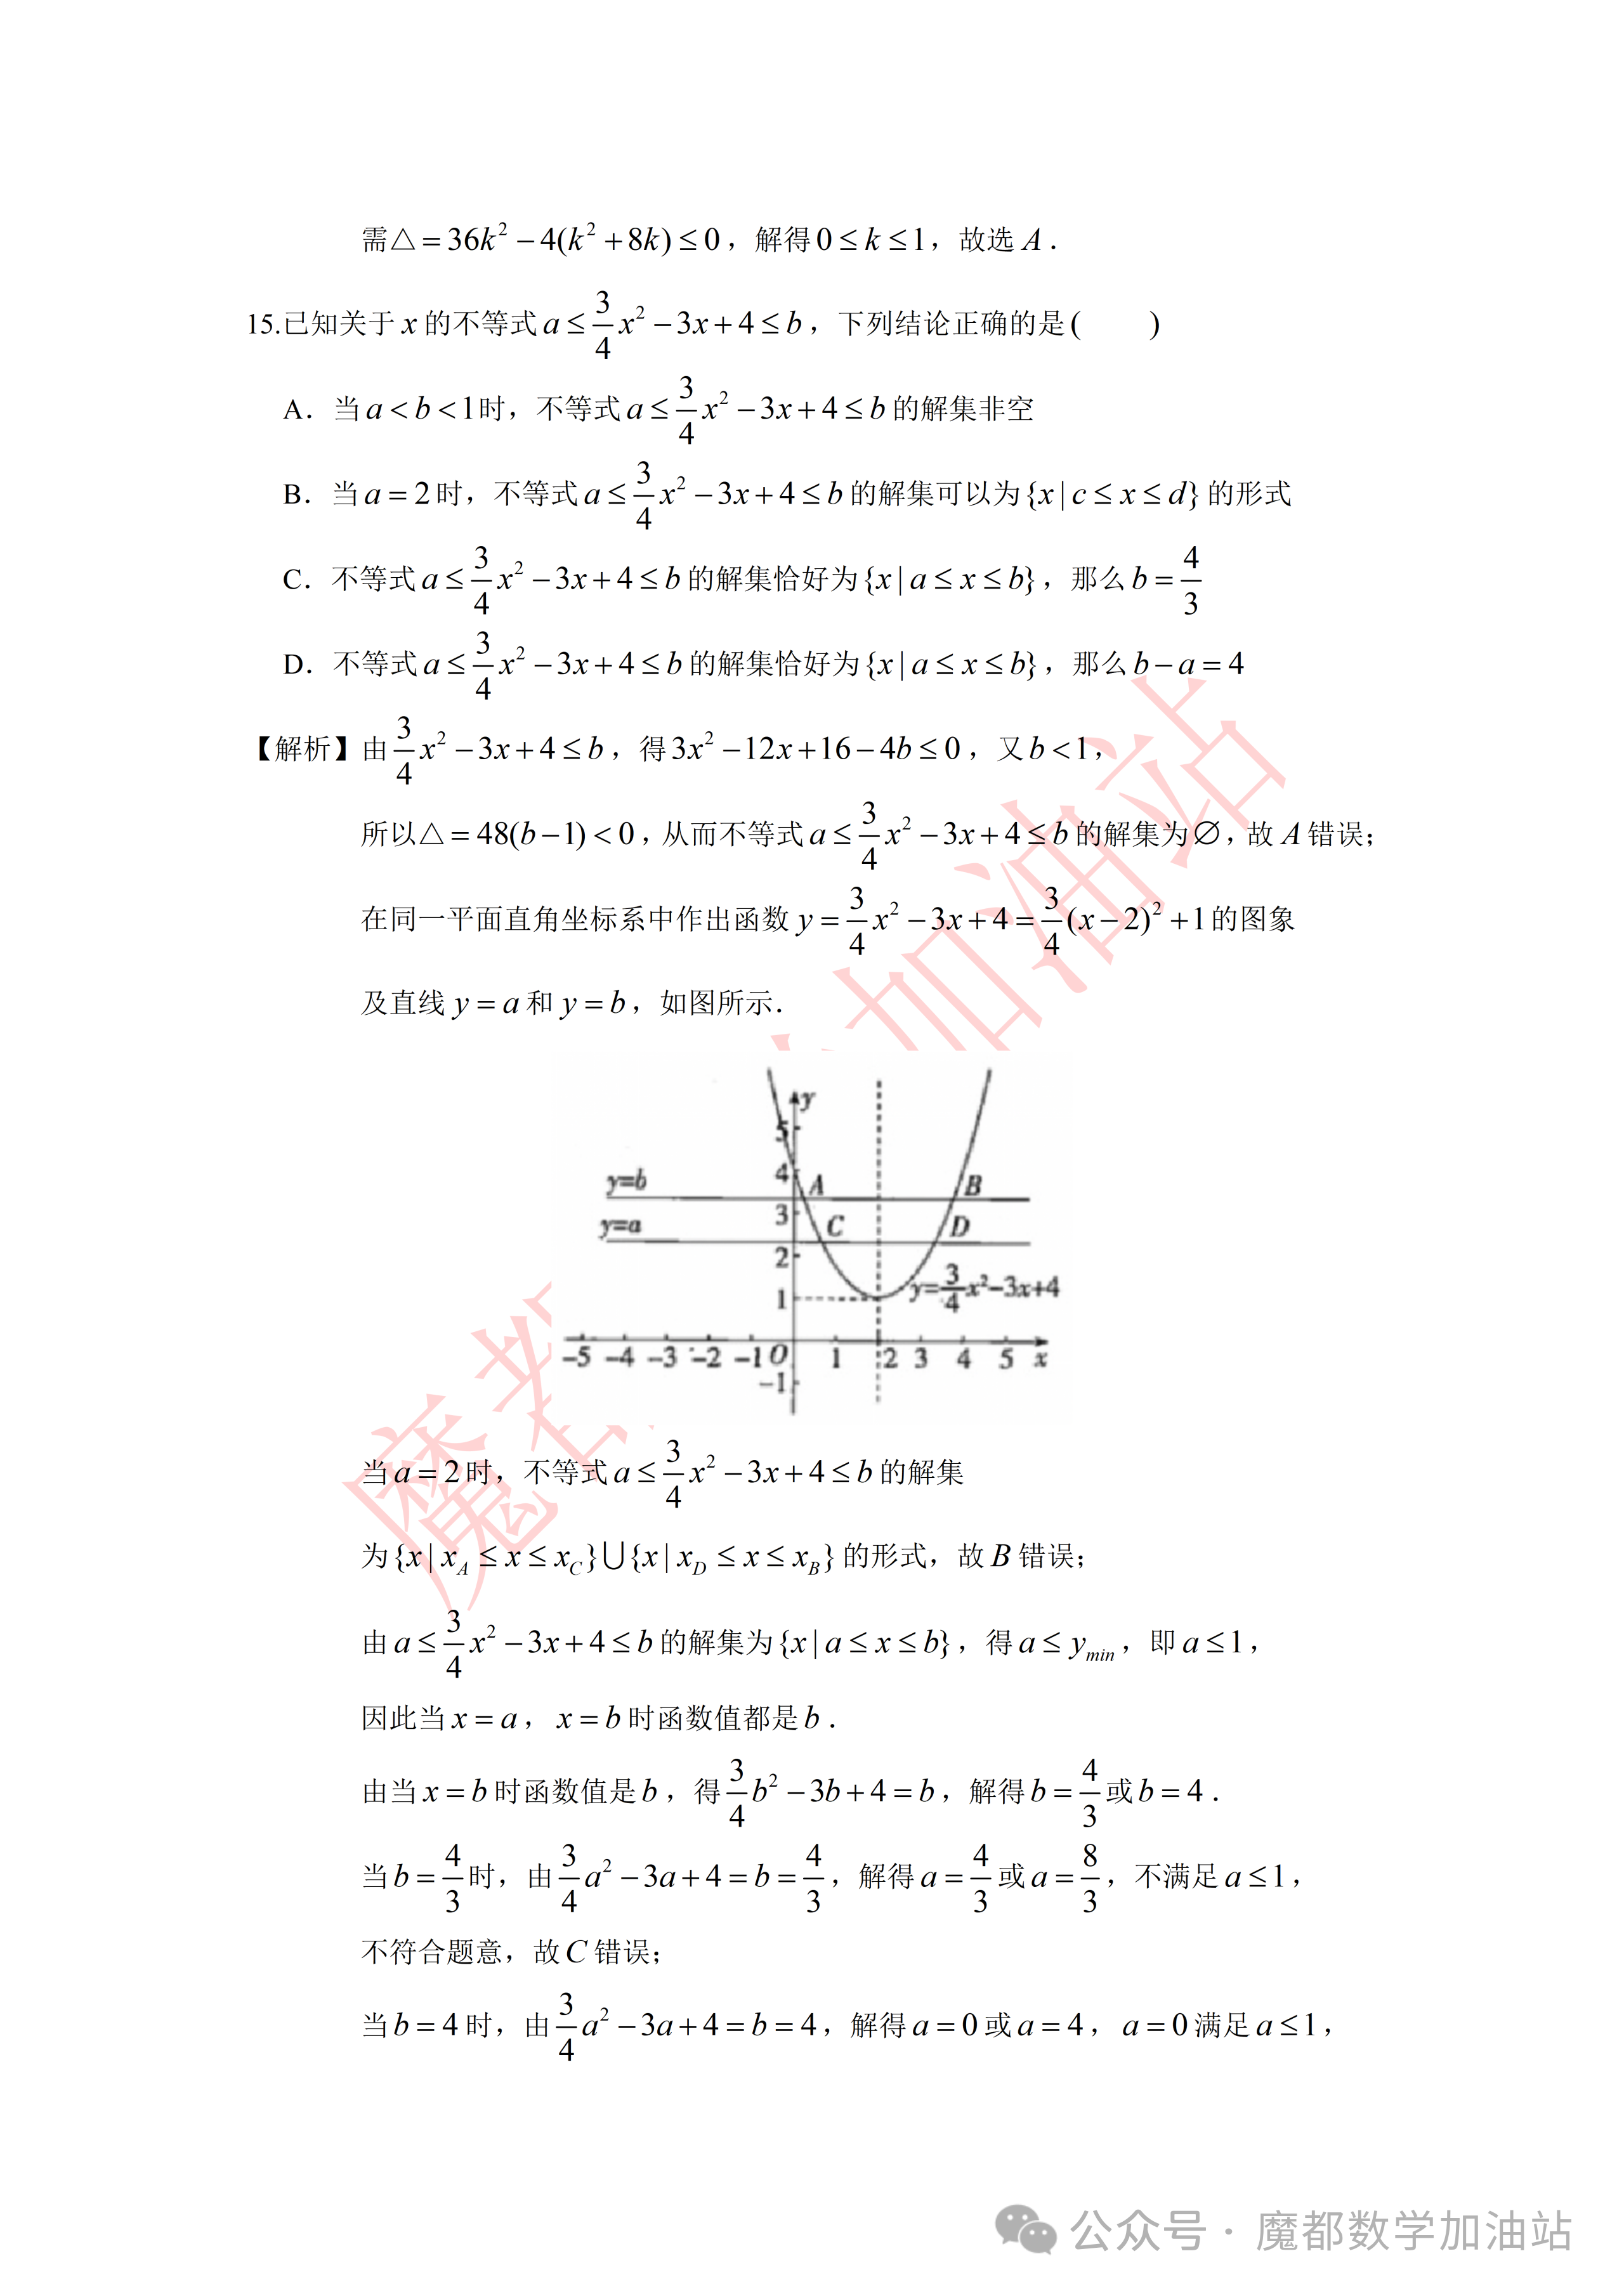
\includegraphics[width=.55\linewidth,trim=900bp 1400bp 760bp 1680bp,clip]{../原图/高一46_交附闵行_国庆作业3/05.png}
\end{center}
\step{当 $a=2$ 时，不等式 $a\leqslant\dfrac34x^2-3x+4\leqslant b$ 的解集为
$\{x\mid x_A\leqslant x\leqslant x_C\}\cup\{x\mid x_D\leqslant x\leqslant x_B\}$ 的形式，故 $B$ 错误；}
\step{由 $a\leqslant\dfrac34x^2-3x+4\leqslant b$ 的解集恰好为 $\{x\mid a\leqslant x\leqslant b\}$ 的形式，得 $a\leqslant y_{\min}$，即 $a\leqslant1$，}
\step{因为当 $x=a$、$x=b$ 时函数值都是 $b$，当 $x=a$ 时，$\dfrac34a^2-3a+4=b$；当 $x=b$ 时，$\dfrac34b^2-3b+4=b$，}
\step{解得 $b=\dfrac43$ 或 $b=4$，}
\step{当 $b=\dfrac43$ 时，由 $\dfrac34a^2-3a+4=b$，解得 $a=\dfrac43$ 或 $a=\dfrac83$，不符合题意，故 $C$ 错误；}
\step{当 $b=4$ 时，由 $\dfrac34a^2-3a+4=b$，解得 $a=0$ 或 $a=4$，$a=0$ 满足 $a\leqslant1$，故 $D$ 正确；}
\step{故选 $D$.}
\solend
\fi

\item 已知 $x$、$y\in(0,+\infty)$，则 $(x-y)^2+2y+1-x+\dfrac4x$ 的最小值为\mbox{（\quad）}

\keepwithprev
A. $1$\qquad B. $2$\qquad C. $3$\qquad D. $4$

\ans{$D$}

\ifanswer
\solbegin
\step{因为 $(x-y)^2+2y+1-x+\dfrac4x=(x-y-1)^2+x+\dfrac4x$，}
\step{当且仅当 $x-y-1=0$，且 $x=\dfrac4x$ 时取等号，}
\step{又因为 $x+\dfrac4x\geqslant2\sqrt{x\cdot\dfrac4x}=4$，当且仅当 $x=2$ 时取等号，}
\step{故选 $D$.}
\solend
\fi

\end{enumerate}

\bigsec{三、解答题}

\begin{enumerate}
\setcounter{enumi}{16}

\item 设集合 $A=\left\{x\middle|\dfrac{x-3}{x-1}<0\right\}$，$B=\{x\mid x^2-2ax+a^2-1>0\}$.
\begin{enumerate}[label=(\arabic*)]
\item 若 $a=3$，求 $A\cup B$；
\item 若“$x\in A$”是“$x\in B$”的充分条件，求实数 $a$ 的取值范围.
\end{enumerate}

\ifanswer
\solbegin
% 注：原卷题干为 a^2-1，故 a=3 时常数项为 8；题干与本步一致。
\stepm{(1)}{当 $a=3$ 时，$B=\{x\mid x^2-6x+8>0\}=\{x\mid x<2\text{ 或 }x>4\}$；}
\step{因为 $A=\left\{x\middle|\dfrac{x-3}{x-1}<0\right\}=\{x\mid(x-1)(x-3)<0\}=\{x\mid1<x<3\}$，}
\step{所以 $A\cup B=\{x\mid x<2\text{ 或 }x>4\}\cup\{x\mid1<x<3\}
=\{x\mid x<3\text{ 或 }x>4\}$.}
\stepm{(2)}{因为“$x\in A$”是“$x\in B$”的充分条件，所以 $A\subseteq B$，}
\step{因 $A=\left\{x\middle|\dfrac{x-3}{x-1}<0\right\}
=\{x\mid(x-1)(x-3)<0\}=\{x\mid1<x<3\}$，}
\step{所以 $A\subseteq B=\{x\mid x<a-1\text{ 或 }x>a+1\}$，}
\step{要使 $A\subseteq B$，需有 $a-1\geqslant3$ 或 $a+1\leqslant1$，}
\step{所以 $a\geqslant4$ 或 $a\leqslant0$，故 $a$ 的取值范围为 $\{a\mid a\geqslant4\text{ 或 }a\leqslant0\}$.}
\solend
\fi

\ansspace[6]

\item 某学校引入种植类劳动教育课程，打算围成如图所示的四块全等的长方形田地种植不同种类的蔬菜，其中一面可以利用原有的墙（足够长），其他各面需要用篱笆围成，设其中一块田地为矩形 $ABCD$.

\begin{center}
% 原图第 6 页配图直接裁取。
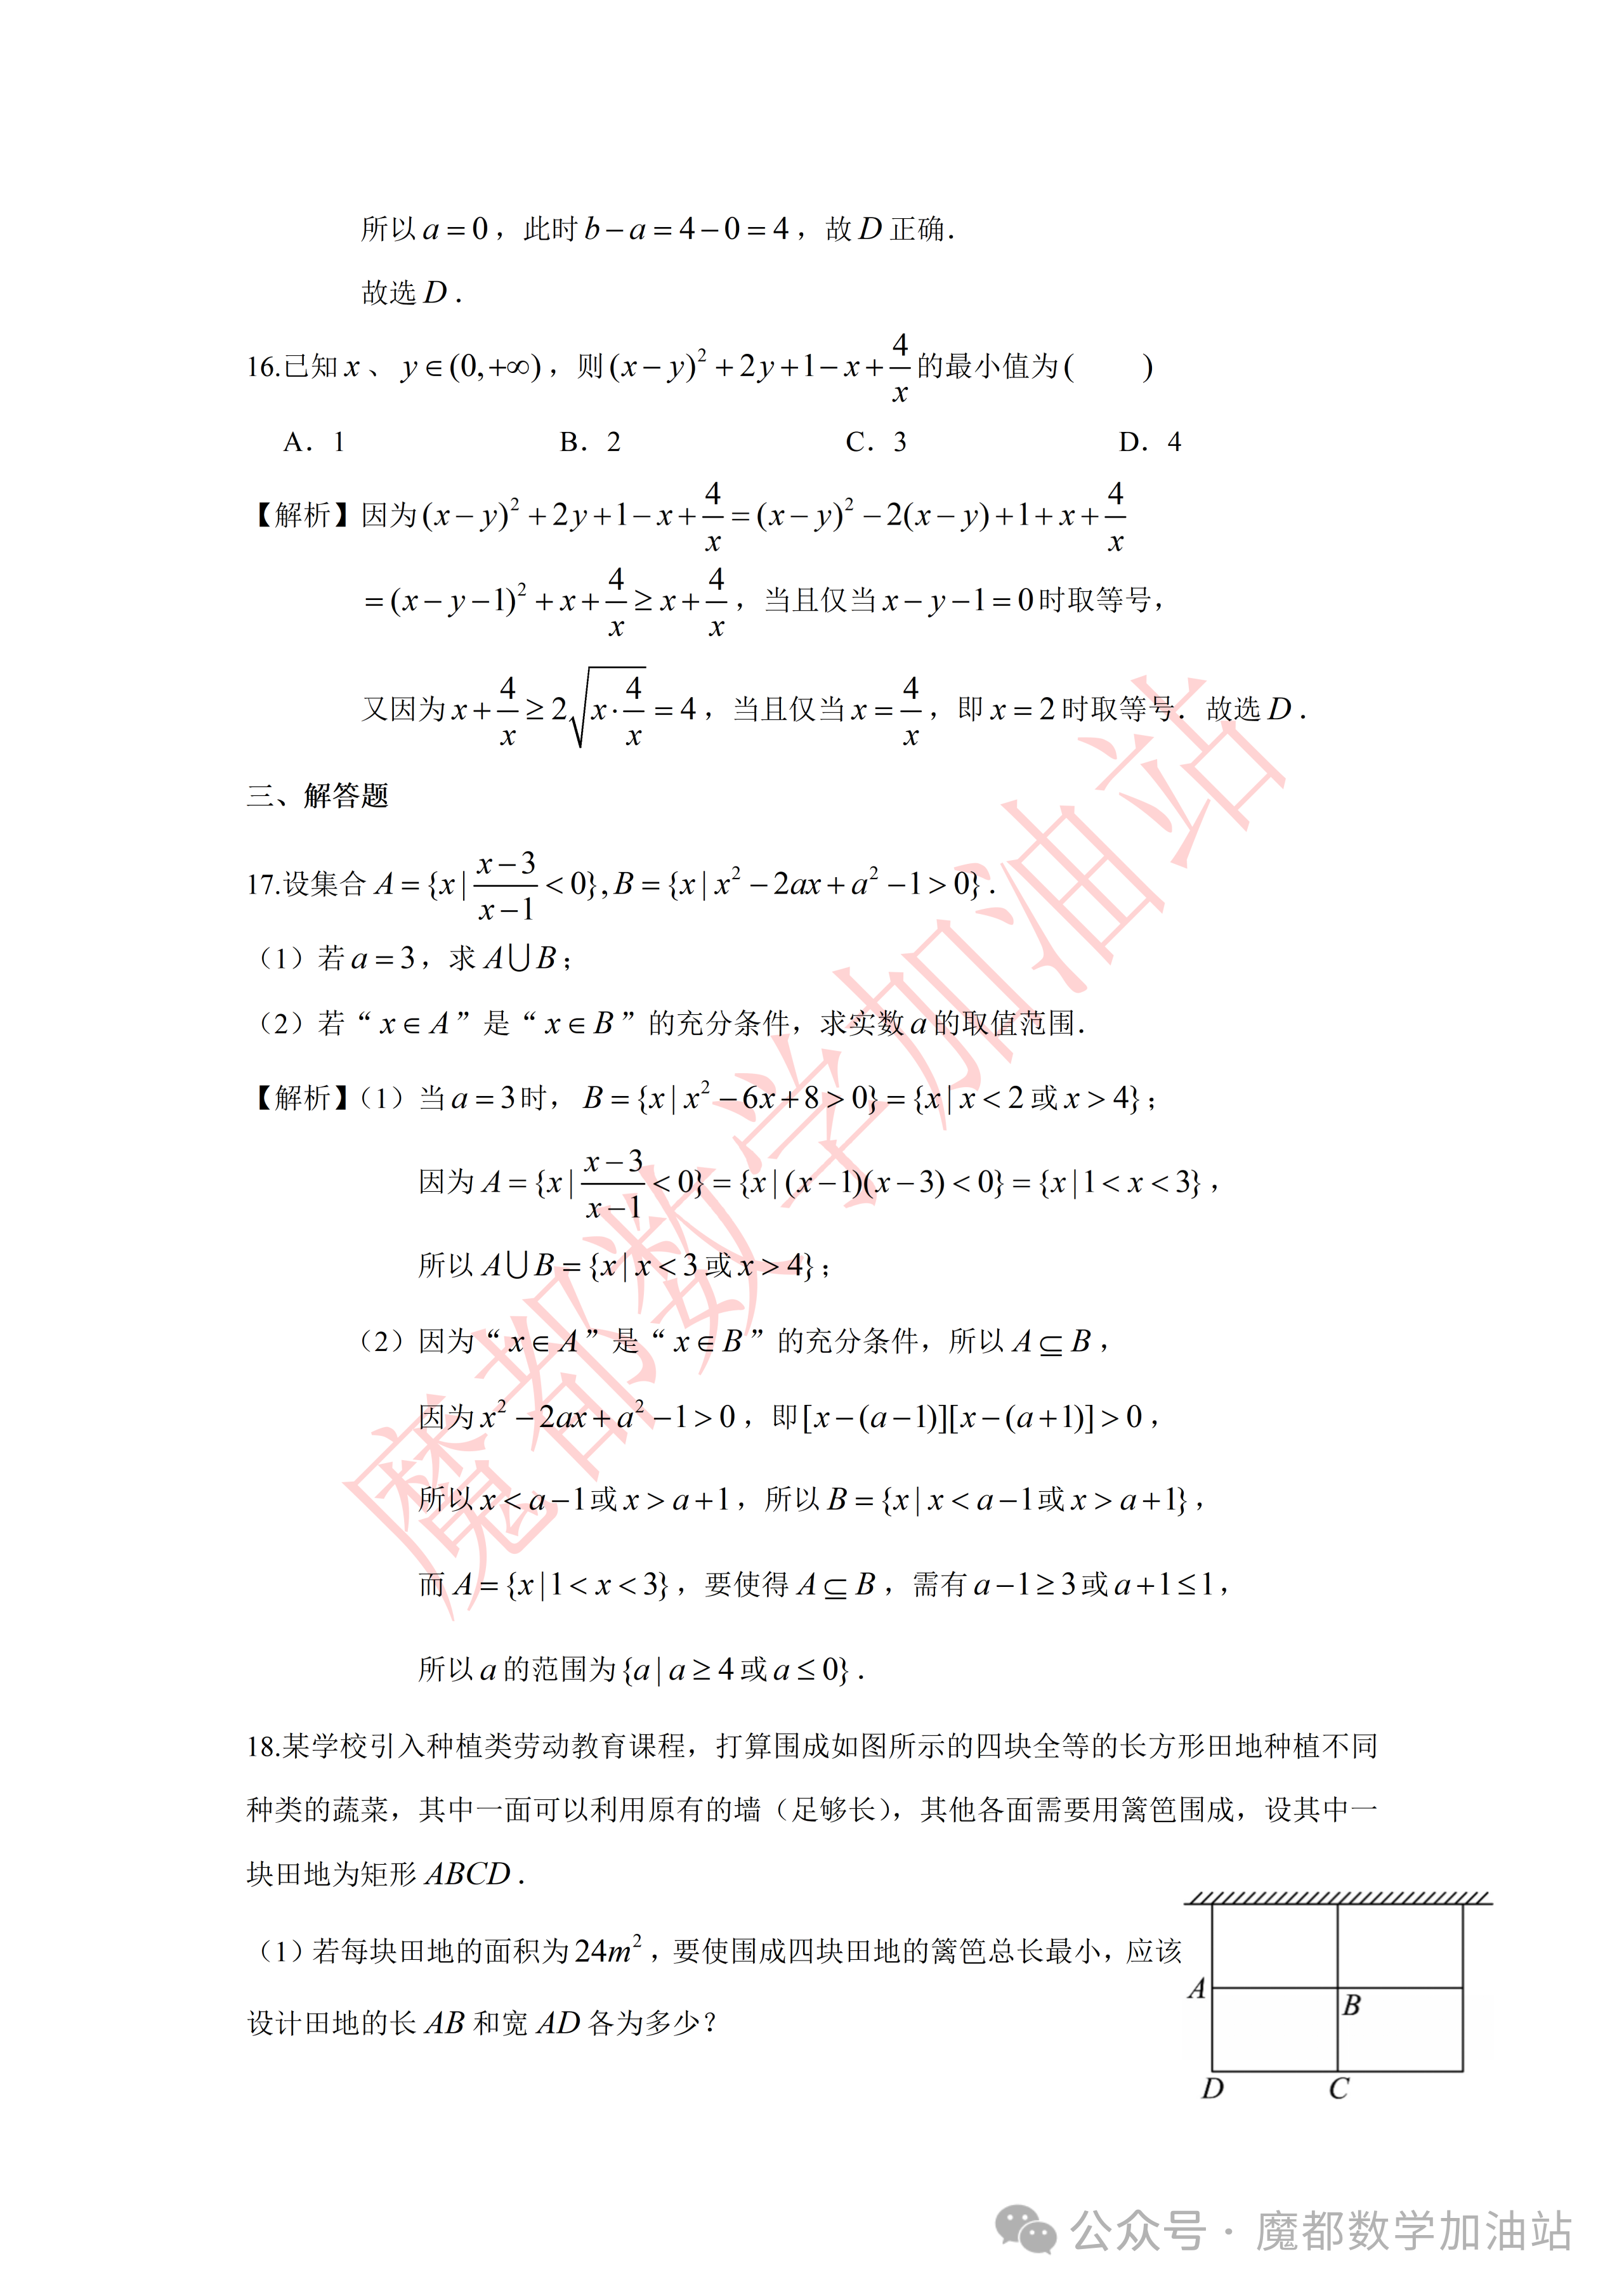
\includegraphics[width=.33\linewidth,trim=1866bp 220bp 210bp 2960bp,clip]{../原图/高一46_交附闵行_国庆作业3/06.png}
\end{center}

\begin{enumerate}[label=(\arabic*)]
\item 若每块田地的面积为 $24\,\text{m}^2$，要使围成四块田地的篱笆总长最小，应该设计田地的长 $AB$ 和宽 $AD$ 各为多少？
\item 现有 $40\,\text{m}$ 长的篱笆，要使每块田地的面积最大，应该设计田地的长 $AB$ 和宽 $AD$ 各为多少？
\end{enumerate}

\ifanswer
\solbegin
\stepm{(1)}{设 $AB$ 长为 $x\,\text{m}$，$AD$ 宽为 $y\,\text{m}$，由题意得 $xy=24$，篱笆总长为 $4x+6y$，}
\step{$4x+6y\geqslant2\sqrt{4x\cdot6y}=2\sqrt{24xy}=48$，}
\step{当且仅当 $4x=6y$ 时取等号，解得 $x=6$，$y=4$，}
\step{所以田地的长 $AB$ 为 $6\,\text{m}$，宽 $AD$ 为 $4\,\text{m}$.}
\stepm{(2)}{设 $AB$ 长为 $a\,\text{m}$，$AD$ 宽为 $b\,\text{m}$，由篱笆总长 $4a+6b=40$，即 $2a+3b=20$，}
\step{将 $a=\dfrac{20-3b}{2}$ 代入每块田地面积 $ab$，得 $ab=\dfrac12b(20-3b)=-\dfrac32b^2+10b$，}
\step{当 $b=\dfrac{10}{3}$ 时，$ab$ 最大，此时 $a=5$，}
\step{所以田地的长 $AB$ 为 $5\,\text{m}$，宽 $AD$ 为 $\dfrac{10}{3}\,\text{m}$.}
\solend
\fi

\ansspace[8]

\item 已知 $x_1$、$x_2$ 是一元二次方程 $4kx^2-4kx+k+1=0$ 的两个不等实数根.
\begin{enumerate}[label=(\arabic*)]
\item 若 $x_1$、$x_2$ 均为正根，求实数 $k$ 的取值范围；
\item 求使 $\dfrac{x_1}{x_2}+\dfrac{x_2}{x_1}-2$ 的值为整数 $k$ 的整数值.
\end{enumerate}

\ifanswer
\solbegin
\stepm{(1)}{由题意，$x_1$、$x_2$ 是方程 $4kx^2-4kx+k+1=0$ 的两个不等实数根，}
\step{故 $k\neq0$，$\Delta=(-4k)^2-16k(k+1)>0$，得 $-16k>0$，所以 $k<0$，}
\step{又 $x_1+x_2=1$，$x_1x_2=\dfrac{k+1}{4k}>0$，得 $k+1<0$，}
\step{所以 $k$ 的取值范围为 $(-\infty,-1)$.}
\stepm{(2)}{由题意，}
\step{$\dfrac{x_1}{x_2}+\dfrac{x_2}{x_1}-2
=\dfrac{x_1^2+x_2^2-2x_1x_2}{x_1x_2}
=\dfrac{(x_1+x_2)^2-4x_1x_2}{x_1x_2}$，}
\step{又 $x_1+x_2=1$，$x_1x_2=\dfrac{k+1}{4k}$，}
\step{则 $\dfrac{x_1}{x_2}+\dfrac{x_2}{x_1}-2=-\dfrac4{k+1}$，}
\step{由于 $-\dfrac4{k+1}$ 为整数，故 $k+1$ 只能取 $\pm1$、$\pm2$、$\pm4$，又 $k<-1$，}
\step{所以整数 $k$ 的值为 $-2$、$-3$、$-5$.}
\solend
\fi

\ansspace[8]

\item 已知 $a>0$，$b>0$，且 $2a+3b=3$.
\begin{enumerate}[label=(\arabic*)]
\item 求 $ab$ 的最大值；
\item 求 $a-\dfrac1{6b}$ 的最大值；
\item 求 $\dfrac2a+\dfrac3{b+1}$ 的最小值.
\end{enumerate}

\ifanswer
\solbegin
\stepm{(1)}{由 $2a+3b=3$，得 $3=2a+3b\geqslant2\sqrt{6ab}$，}
\step{所以 $ab\leqslant\dfrac38$，当且仅当 $2a=3b=\dfrac32$ 时取等号，}
\step{故 $ab$ 的最大值为 $\dfrac38$.}
\stepm{(2)}{由 $2a+3b=3$，得 $a=\dfrac32-\dfrac32b$，}
\step{则 $a-\dfrac1{6b}=\dfrac32-\dfrac32b-\dfrac1{6b}$，}
\step{由基本不等式，$\dfrac32b+\dfrac1{6b}\geqslant2\sqrt{\dfrac32b\cdot\dfrac1{6b}}=1$，}
\step{当且仅当 $\dfrac32b=\dfrac1{6b}$，即 $b=\dfrac13$、$a=1$ 时取等号，}
\step{所以 $a-\dfrac1{6b}$ 的最大值为 $\dfrac12$.}
\stepm{(3)}{由 $2a+3b=3$，得 $2a+3(b+1)=6$，}
\step{$\dfrac2a+\dfrac3{b+1}
=\dfrac16\left(2a+3(b+1)\right)\left(\dfrac2a+\dfrac3{b+1}\right)$}
\step{$=\dfrac16\left(13+\dfrac{6(b+1)}a+\dfrac{6a}{b+1}\right)
\geqslant\dfrac16\left(13+2\sqrt{\dfrac{6(b+1)}a\cdot\dfrac{6a}{b+1}}\right)=\dfrac{25}{6}$，}
\step{当且仅当 $a=b+1$，即 $a=\dfrac65$、$b=\dfrac15$ 时取等号，}
\step{所以 $\dfrac2a+\dfrac3{b+1}$ 的最小值为 $\dfrac{25}{6}$.}
\solend
\fi

\ansspace[8]

\item 已知 $U=\R$ 为全集，集合 $A=\{s^2+3t^2\mid s,t\in U\}$.
\begin{enumerate}[label=(\arabic*)]
\item 设 $U=\{1,3,5\}$，求集合 $A$ 的元素个数；
\item 设 $U=\Z$，证明：若 $x\in A$，则 $7x\in A$；
\item 设 $U=\R$，$x$、$y\in A$，且 $x=m^2+3n^2$，$y=p^2+3q^2$，若 $mp-3nq=\sqrt3$，求 $x+y+mq+np$ 的最小值.
\end{enumerate}

\ifanswer
\solbegin
\stepm{(1)}{当 $s=1$，$t=1$ 时，$s^2+3t^2=1+3=4$；}
\step{当 $s=1$，$t=3$ 时，$s^2+3t^2=1+27=28$；}
\step{当 $s=1$，$t=5$ 时，$s^2+3t^2=1+75=76$；}
\step{当 $s=3$，$t=1$ 时，$s^2+3t^2=9+3=12$；}
\step{当 $s=3$，$t=3$ 时，$s^2+3t^2=9+27=36$；}
\step{当 $s=3$，$t=5$ 时，$s^2+3t^2=9+75=84$；}
\step{当 $s=5$，$t=1$ 时，$s^2+3t^2=25+3=28$；}
\step{当 $s=5$，$t=3$ 时，$s^2+3t^2=25+27=52$；}
\step{当 $s=5$，$t=5$ 时，$s^2+3t^2=25+75=100$，}
\step{所以 $A=\{4,12,28,36,52,76,84,100\}$，有 $8$ 个元素.}
\stepm{(2)}{因为 $U=\Z$，$x\in A$，设 $x=s^2+3t^2$，}
\step{则 $7x=7(s^2+3t^2)=(2s+3t)^2+3(s-2t)^2\in A$，}
\step{所以 $7x\in A$.}
\stepm{(3)}{因为 $x=m^2+3n^2$，$y=p^2+3q^2$，}
\step{$xy=(m^2+3n^2)(p^2+3q^2)=3(mq+np)^2+(mp-3nq)^2$，}
\step{设 $mq+np=b$，则 $xy=3b^2+3$，所以 $y=\dfrac{3b^2+3}{x}$，}
\step{于是 $x+y+mq+np=x+\dfrac{3b^2+3}{x}+b\geqslant2\sqrt{3b^2+3}+b$，}
\step{设 $2\sqrt{3b^2+3}+b=t$，整理得 $11b^2+2bt+12-t^2=0$，}
\step{判别式法，$\Delta=4t^2-44(12-t^2)\geqslant0$，得 $t\geqslant\sqrt{11}$，}
\step{即 $(x+y+mq+np)_{\min}=\sqrt{11}$，所以 $x+y+mq+np$ 的最小值为 $\sqrt{11}$.}
\solend
\fi

\ansspace*[10]

\end{enumerate}

\end{document}
"
%
% 原始材料：微信公众号“魔都数学加油站”，作者破晓，2026-10-02 17:56 发布。
% 原文标题：“27学年高一46——2026-2027你那上海市交附闵行高一上国庆作业3”
% （公众号标题中的“你那”照录，系原文标题字样）；原文链接：
% http://mp.weixin.qq.com/s?__biz=Mzg4ODU1ODMxOQ==&mid=2247591657&idx=3&sn=a894d1a16611283a61b3eaba32a3f24c&chksm=cee83366c6a55381b370069f84ef63d20251f94608bb37cc4ec2d66227401bd147f4f6bd8256&scene=126&sessionid=1790935402&subscene=7&clicktime=1790937618&enterid=1790937618#rd
% 正文为 9 张 PNG 页，按页序读取原图；第 01、02、07 页 4762×6735，
% 第 03—06、08、09 页 2560×3620。卷面标题照原卷印作“2026-2027 年交附闵行高一上国庆作业 3”。
% 原文从第 3 题起，题号照原卷保留；正文为讲评版，答案、解析依原卷顺序录入。
% 水印及页脚公众号标识不录入。卷面插图直接裁取对应原图页，不另制图片文件。
%
% 与原卷的排版差异：
%   ① 原卷按“一、填空题”“二、选择题”“三、解答题”分节，本稿沿用原节与原题号，
%      只改排为全稿统一的大节样式；
%   ② 原卷答案与解析依页面位置分布，本稿按 common.sty 统一置于答案版；
%   ③ 原卷副标题未印，本稿按“知识模块”口径标作“集合与常用逻辑用语、不等式”。
%
% 原卷存疑一处（照抄未改，见第 12 题题干及解析处注释）：
%   第 12 题题干同时给出 x∈Z，却称不等式组有“50 个不等的实数解”；解析按整数根计数。
%   此处题干与解析的原文不一致，本稿均照录。
% 第 17 题曾疑似有常数项不一致：复核原图题干为 a^2-1，a=3 时常数项确为 8，
% 与解析相符；不将其记作原卷错误。
%
\documentclass[a4paper,11pt]{article}
\usepackage{common}

\begin{document}

\examtitlest[3]{2026--2027 年交附闵行高一上国庆作业 3}{集合与常用逻辑用语、不等式}

\bigsec{一、填空题}

\begin{enumerate}
\setcounter{enumi}{2}

\item 不等式 $\dfrac{x^2-10}{x+2}\geqslant1$ 的解集为\blankline[4.4em].

\ifanswer
\ans{$\{x\mid-3\leqslant x<-2\text{ 或 }x\geqslant4\}$}
\solbegin
\step{不等式 $\dfrac{x^2-10}{x+2}\geqslant1$，移项得 $\dfrac{x^2-10}{x+2}-1\geqslant0$，}
\step{通分得 $\dfrac{x^2-x-12}{x+2}\geqslant0$，即 $\dfrac{(x-4)(x+3)}{x+2}\geqslant0$，}
\step{解得 $-3\leqslant x<-2$ 或 $x\geqslant4$，}
\step{故不等式的解集为 $\{x\mid-3\leqslant x<-2\text{ 或 }x\geqslant4\}$.}
\solend
\fi

\item $|x-3|+|x-5|\geqslant2$，当等号成立时，$x$ 的范围是\blankline[4.4em].

\ifanswer
\ans{$[3,5]$}
\fi

\item 若直角三角形斜边长等于 $4\sqrt2\,\text{cm}$，则直角三角形面积的最大值为\blankline[4.4em].

\ifanswer
\solbegin
\step{设 $Rt\triangle ABC$ 中，$C=90^\circ$，则 $c=\sqrt{a^2+b^2}=4\sqrt2$，所以 $a^2+b^2=32$，}
\step{由基本不等式得 $a^2+b^2\geqslant2ab$，当且仅当 $a=b=4$ 时取等号，}
\step{所以 $\triangle ABC$ 的面积 $S=\dfrac12ab\leqslant8$，}
\step{当且仅当 $a=b=4$ 时，$\triangle ABC$ 的面积最大值为 $8$.}
\solend
\fi

\item 不等式 $(x-1)(2-x)>0$ 的解集为\blankline[4.4em].

\ifanswer
\solbegin
\step{$(x-1)(2-x)>0\Rightarrow(x-1)(x-2)<0$，}
\step{故不等式的解集为 $\{x\mid1<x<2\}$.}
\solend
\fi

\item 已知集合 $A=\{1,2\}$，$B=\{x\mid x^2-2mx+m=0\}$，$A\cup B=A$，则实数 $m$ 的取值范围为\blankline[4.4em].

\ifanswer
\solbegin
\step{因为 $A\cup B=A$，所以 $B\subseteq A$，}
\step{当 $B=\varnothing$ 时，$\Delta=(-2m)^2-4m<0$，解得 $0<m<1$，}
\step{当 $B$ 为单元素集时，$\Delta=0$，解得 $m=0$ 或 $m=1$，}
\step{当 $m=0$ 时，方程 $x^2=0$，解得 $x=0$，此时 $B=\{0\}$，不满足 $B\subseteq A$；}
\step{当 $m=1$ 时，方程 $x^2-2x+1=0$，解得 $x=1$，此时 $B=\{1\}$，满足 $B\subseteq A$；}
\step{当 $B=\{1,2\}$ 时，由韦达定理得 $1+2=2m$，$1\times2=m$，无解，}
\step{综上所述，实数 $m$ 的取值范围为 $\{m\mid0<m\leqslant1\}$.}
\solend
\fi

\item 设 $a$、$b$、$c\in\R^+$，若 $a+b+c=1$，则 $\dfrac1a+\dfrac1b+\dfrac1c\geqslant$\blankline[4.4em].

\ifanswer
\solbegin
\step{因为 $a$、$b$、$c\in\R^+$，且 $a+b+c=1$，}
\step{所以 $\dfrac1a+\dfrac1b+\dfrac1c=(a+b+c)\left(\dfrac1a+\dfrac1b+\dfrac1c\right)$}
\step{$=3+\dfrac ab+\dfrac ba+\dfrac ac+\dfrac ca+\dfrac bc+\dfrac cb$，}
\step{由基本不等式得 $\dfrac ab+\dfrac ba\geqslant2$，$\dfrac ac+\dfrac ca\geqslant2$，$\dfrac bc+\dfrac cb\geqslant2$，}
\step{所以 $\dfrac1a+\dfrac1b+\dfrac1c\geqslant9$，当且仅当 $a=b=c=\dfrac13$ 时取等号，}
\step{所以 $\dfrac1a+\dfrac1b+\dfrac1c$ 的最小值为 $9$.}
\solend
\fi

\item 已知 $-1\leqslant x+y\leqslant2$，$-2\leqslant x-y\leqslant1$，则 $x-2y$ 的范围为\blankline[4.4em].

\ifanswer
\solbegin
\step{设 $x-2y=m(x+y)+n(x-y)$，}
\step{则 $x-2y=(m+n)x+(m-n)y$，所以 $m+n=1$，$m-n=-2$，}
\step{解得 $m=-\dfrac12$，$n=\dfrac32$，}
\step{所以 $x-2y=-\dfrac12(x+y)+\dfrac32(x-y)$，}
\step{因为 $-1\leqslant x+y\leqslant2$，$-2\leqslant x-y\leqslant1$，}
\step{所以 $-4\leqslant x-2y\leqslant2$，即 $x-2y$ 的范围为 $[-4,2]$.}
\solend
\fi

\item 设集合 $A=\{1,2,m\}$，其中 $m$ 为实数，令 $B=\{a^2\mid a\in A\}$，$C=A\cup B$. 若 $C$ 中所有元素之和为 $6$，则 $C$ 中的所有元素之积为\blankline[4.4em].

\ifanswer
\solbegin
\step{因为 $A=\{1,2,m\}$，所以 $B=\{a^2\mid a\in A\}=\{1,4,m^2\}$，$m\neq1$，$m\neq2$，}
\step{又 $C=A\cup B$，所以 $1\in C$，$4\in C$，$m^2\in C$，}
\step{若 $m^2=1$，则 $m=-1$ 或 $m=1$（舍），当 $m=-1$ 时，$C=\{1,2,4,-1\}$，$C$ 中所有元素之和为 $6$，}
\step{此时 $C$ 中所有元素之积为 $-8$；}
\step{若 $m^2=2$，则 $m=-\sqrt2$ 或 $m=\sqrt2$，$C$ 中所有元素之和不符合题意；}
\step{若 $m^2=4$，则 $m=-2$ 或 $m=2$，此时 $C=\{1,2,4,-2\}$ 或 $C=\{1,2,4\}$，所有元素之和不符合题意；}
\step{若 $m^2\neq1$，$m^2\neq2$，$m^2\neq4$，则 $C=\{1,2,4,m,m^2\}$，}
\step{所以 $1+2+4+m+m^2=6$，即 $m^2+m+1=0$，无解，}
\step{综上所述，$C$ 中所有元素之积为 $-8$.}
\solend
\fi

\item 若对任意实数 $x>0$，$y>0$，不等式 $x+\sqrt{xy}\leqslant a(x+y)$ 恒成立，则实数 $a$ 的最小值为\blankline[4.4em].

\ifanswer
\solbegin
\step{由不等式 $x+\sqrt{xy}\leqslant a(x+y)$ 对任意实数 $x>0$，$y>0$ 恒成立，}
\step{得 $a\geqslant\dfrac{x+\sqrt{xy}}{x+y}$，}
\step{设 $\sqrt{\dfrac yx}=t>0$，则 $a\geqslant\dfrac{1+t}{1+t^2}$，}
\step{$\dfrac{1+t}{1+t^2}\leqslant\dfrac{\sqrt2+1}{2}$，当且仅当 $t=\sqrt2-1$ 时取等号，}
\step{所以实数 $a$ 的最小值为 $\dfrac{\sqrt2+1}{2}$.}
\solend
\fi

% 注：原卷题干给出 x∈Z，却写“实数解”；解析按整数解计数，题干与解析不一致，照录未改。
\item 若关于 $x$ 的不等式组
$\begin{cases}x^2-3mx\geqslant4m^2\\-20<x<120\end{cases}$（$x\in\Z,m>0$）恰有 $50$ 个不等的实数解，则 $m$ 的取值范围为\blankline[4.4em]（结果用区间表示）.

\ifanswer
\solbegin
\step{由 $x^2-3mx\geqslant4m^2$ 以及 $m>0$，解得 $x\leqslant-m$ 或 $x\geqslant4m$，}
\step{由原不等式组恰有 $50$ 个不等的实数解，可画出如下解集区间：}
\begin{center}
% 原图第 4 页数轴图直接裁取。
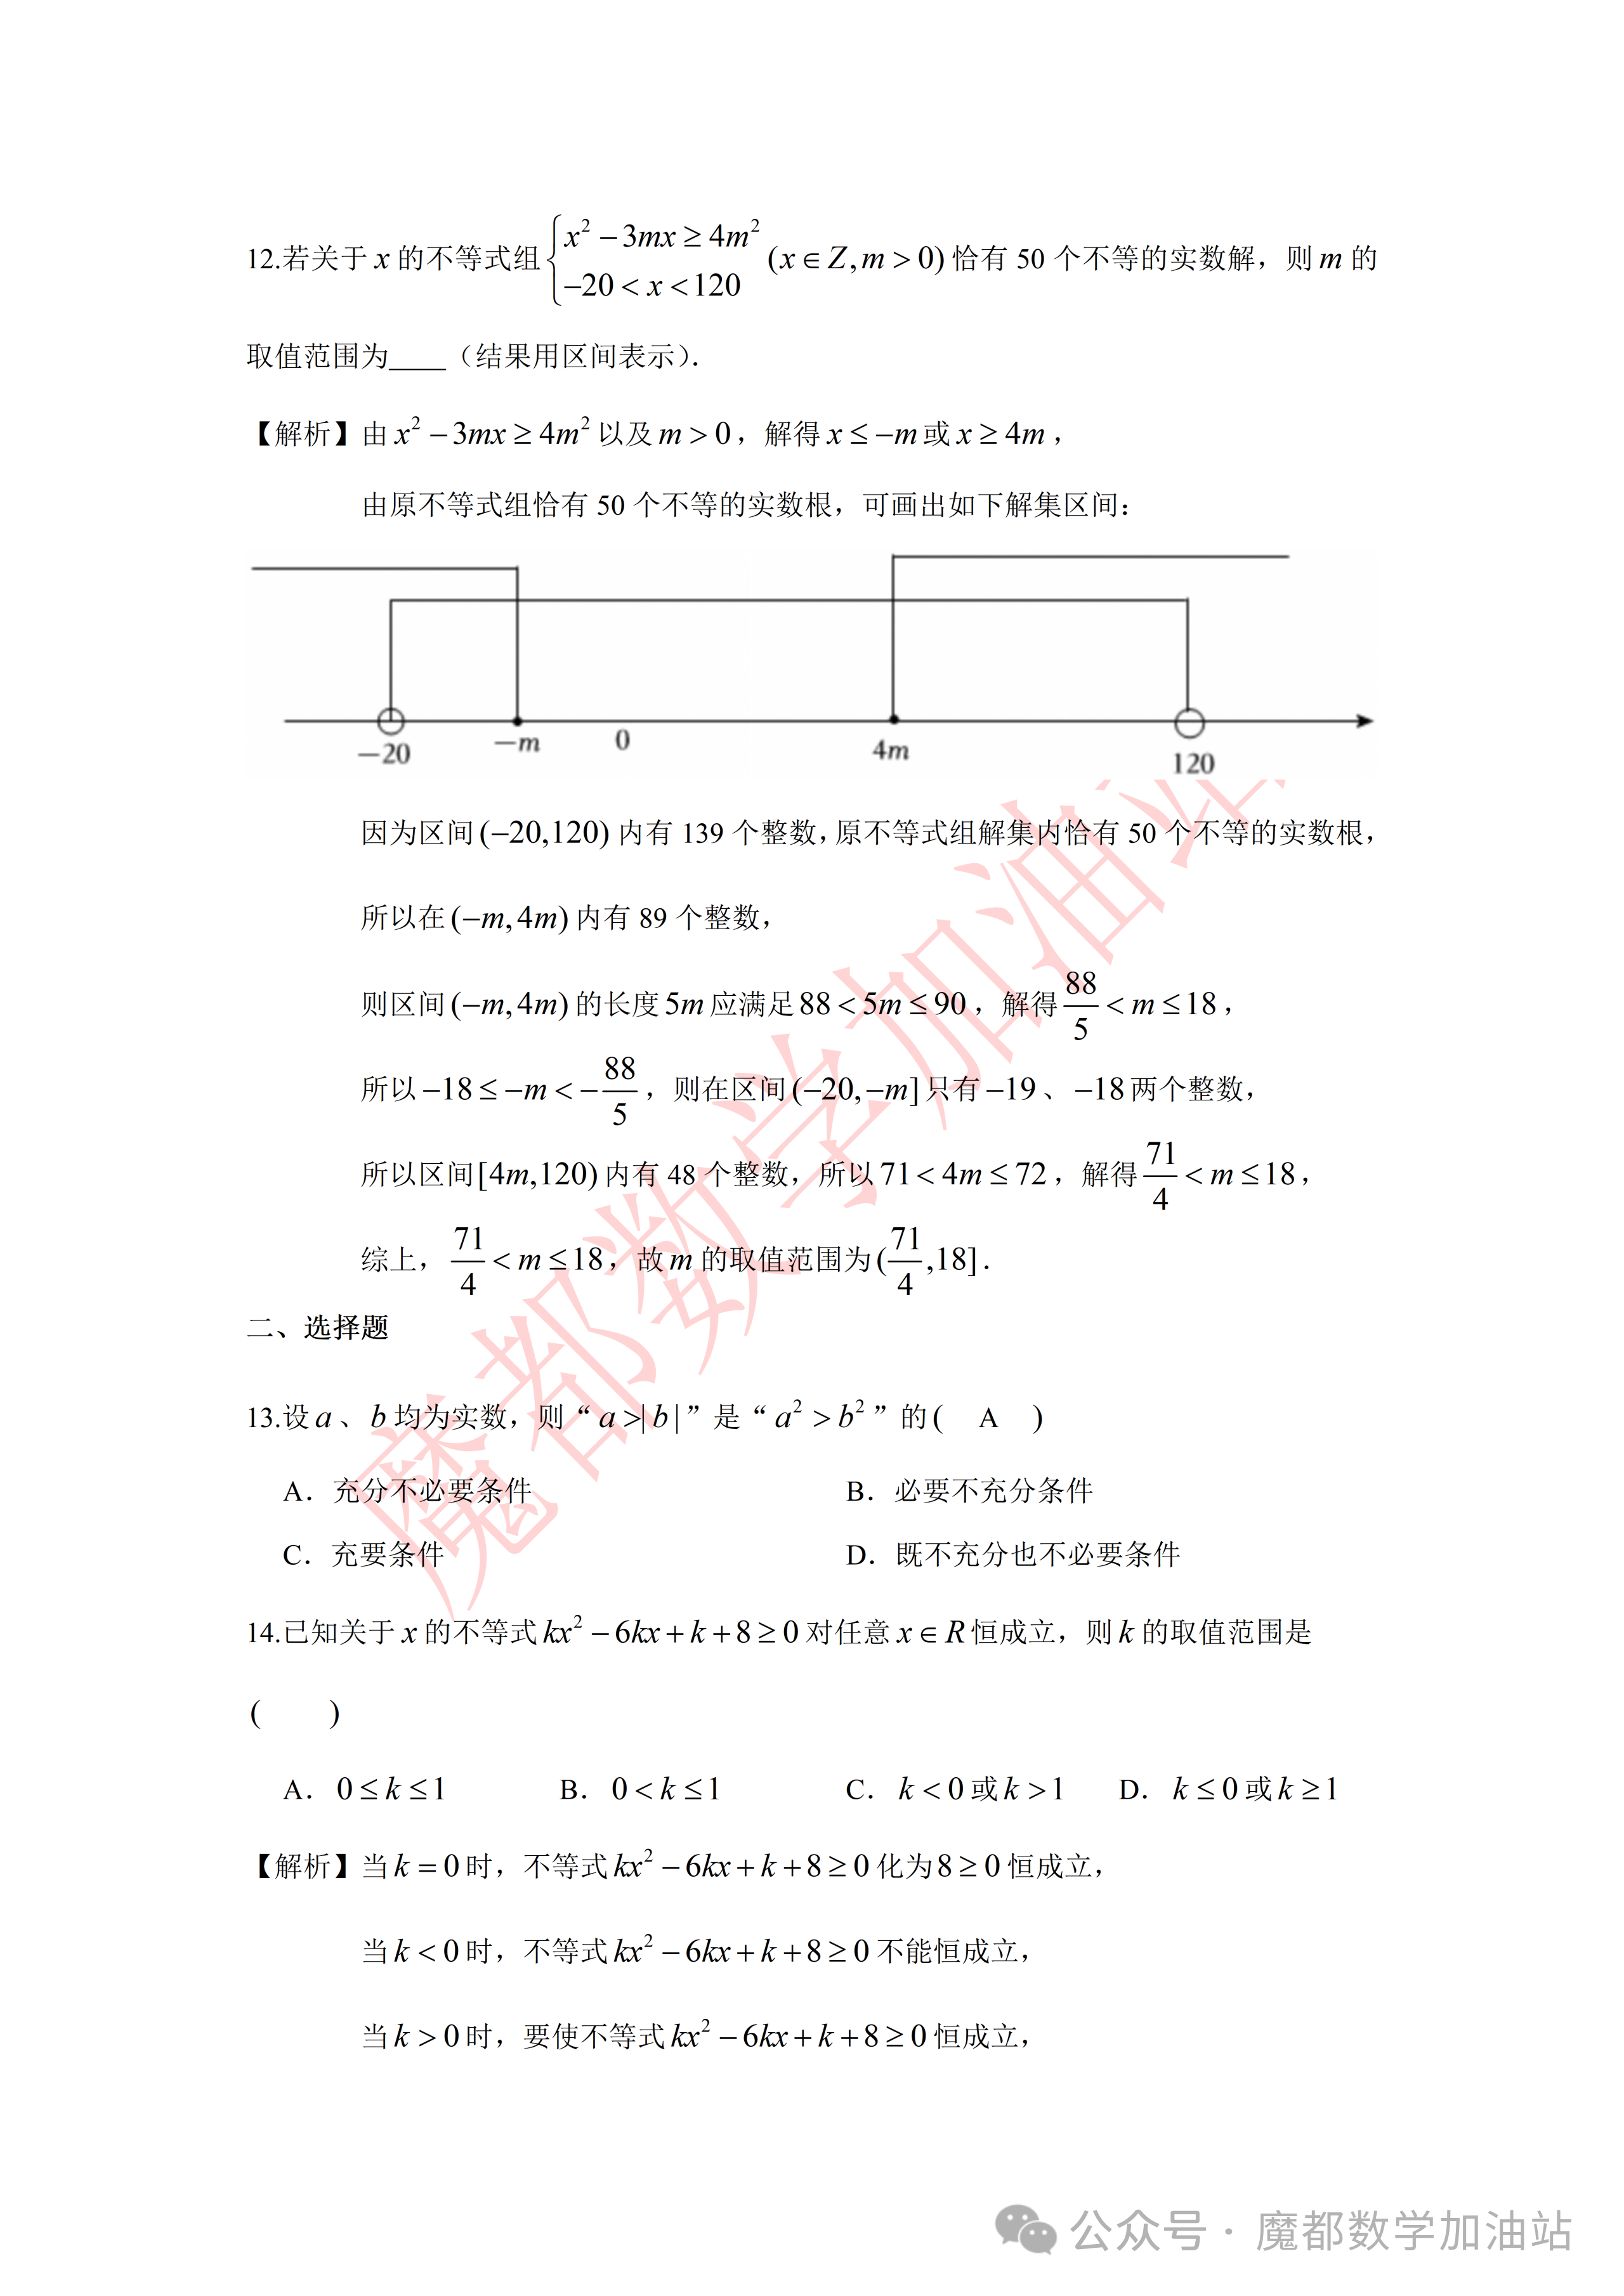
\includegraphics[width=.88\linewidth,trim=400bp 2410bp 320bp 860bp,clip]{../原图/高一46_交附闵行_国庆作业3/04.png}
\end{center}
\step{因为区间 $(-20,120)$ 内有 $139$ 个整数，原不等式组解集内有 $50$ 个不等的整数根，}
\step{所以在区间 $(-m,4m)$ 内有 $89$ 个整数，}
\step{则区间 $(-m,4m)$ 的长度 $5m$ 应满足 $88<5m\leqslant90$，解得 $\dfrac{88}{5}<m\leqslant18$，}
% 注：原卷题干称“实数解”，本行及后文按原卷解析照录为整数根计数。
\step{所以 $-18\leqslant-m<-\dfrac{88}{5}$，则在区间 $(-20,-m]$ 内有 $-19$、$-18$ 两个整数，}
\step{所以区间 $[4m,120)$ 内有 $48$ 个整数，}
\step{则 $71<4m\leqslant72$，解得 $\dfrac{71}{4}<m\leqslant18$，}
\step{综上，$\dfrac{71}{4}<m\leqslant18$，故 $m$ 的取值范围为 $\left(\dfrac{71}{4},18\right]$.}
\solend
\fi

\end{enumerate}

\bigsec{二、选择题}

\begin{enumerate}
\setcounter{enumi}{12}

\item 设 $a$、$b$ 均为实数，则“$a>|b|$”是“$a^2>b^2$”的\mbox{（\quad）}

\keepwithprev
A. 充分不必要条件\qquad B. 必要不充分条件

C. 充要条件\qquad\qquad D. 既不充分也不必要条件

\ans{$A$}

\item 已知关于 $x$ 的不等式 $kx^2-6kx+k+8\geqslant0$ 对任意 $x\in\R$ 恒成立，则 $k$ 的取值范围是\mbox{（\quad）}

\keepwithprev
A. $0\leqslant k\leqslant1$\qquad B. $0<k\leqslant1$

C. $k<0$ 或 $k>1$\qquad D. $k\leqslant0$ 或 $k\geqslant1$

\ans{$A$}

\ifanswer
\solbegin
\step{当 $k=0$ 时，不等式 $kx^2-6kx+k+8\geqslant0$ 化为 $8\geqslant0$ 恒成立，}
\step{当 $k<0$ 时，不等式 $kx^2-6kx+k+8\geqslant0$ 不能恒成立，}
\step{当 $k>0$ 时，要使不等式 $kx^2-6kx+k+8\geqslant0$ 恒成立，}
\step{需 $\Delta=36k^2-4(k^2+8k)\leqslant0$，解得 $0\leqslant k\leqslant1$，故选 $A$.}
\solend
\fi

\item 已知关于 $x$ 的不等式 $a\leqslant\dfrac34x^2-3x+4\leqslant b$，下列结论正确的是\mbox{（\quad）}

\keepwithprev
A. 当 $a<b<1$ 时，不等式 $a\leqslant\dfrac34x^2-3x+4\leqslant b$ 的解集非空

B. 当 $a=2$ 时，不等式 $a\leqslant\dfrac34x^2-3x+4\leqslant b$ 的解集可以为 $\{x\mid c\leqslant x\leqslant d\}$ 的形式

C. 不等式 $a\leqslant\dfrac34x^2-3x+4\leqslant b$ 的解集恰好为 $\{x\mid a\leqslant x\leqslant b\}$，那么 $b=\dfrac43$

D. 不等式 $a\leqslant\dfrac34x^2-3x+4\leqslant b$ 的解集恰好为 $\{x\mid a\leqslant x\leqslant b\}$，那么 $b-a=4$

\ans{$D$}

\ifanswer
\solbegin
\step{由 $\dfrac34x^2-3x+4\leqslant b$，得 $3x^2-12x+16-4b\leqslant0$，又 $b<1$，}
\step{所以 $\Delta=144-12(16-4b)=48(b-1)<0$，从而不等式无解，故 $A$ 错误；}
\step{在同一平面直角坐标系中作出函数 $y=\dfrac34x^2-3x+4=\dfrac34(x-2)^2+1$ 的图象及直线 $y=a$ 和 $y=b$，如图所示.}
\begin{center}
% 原图第 5 页解析配图直接裁取。
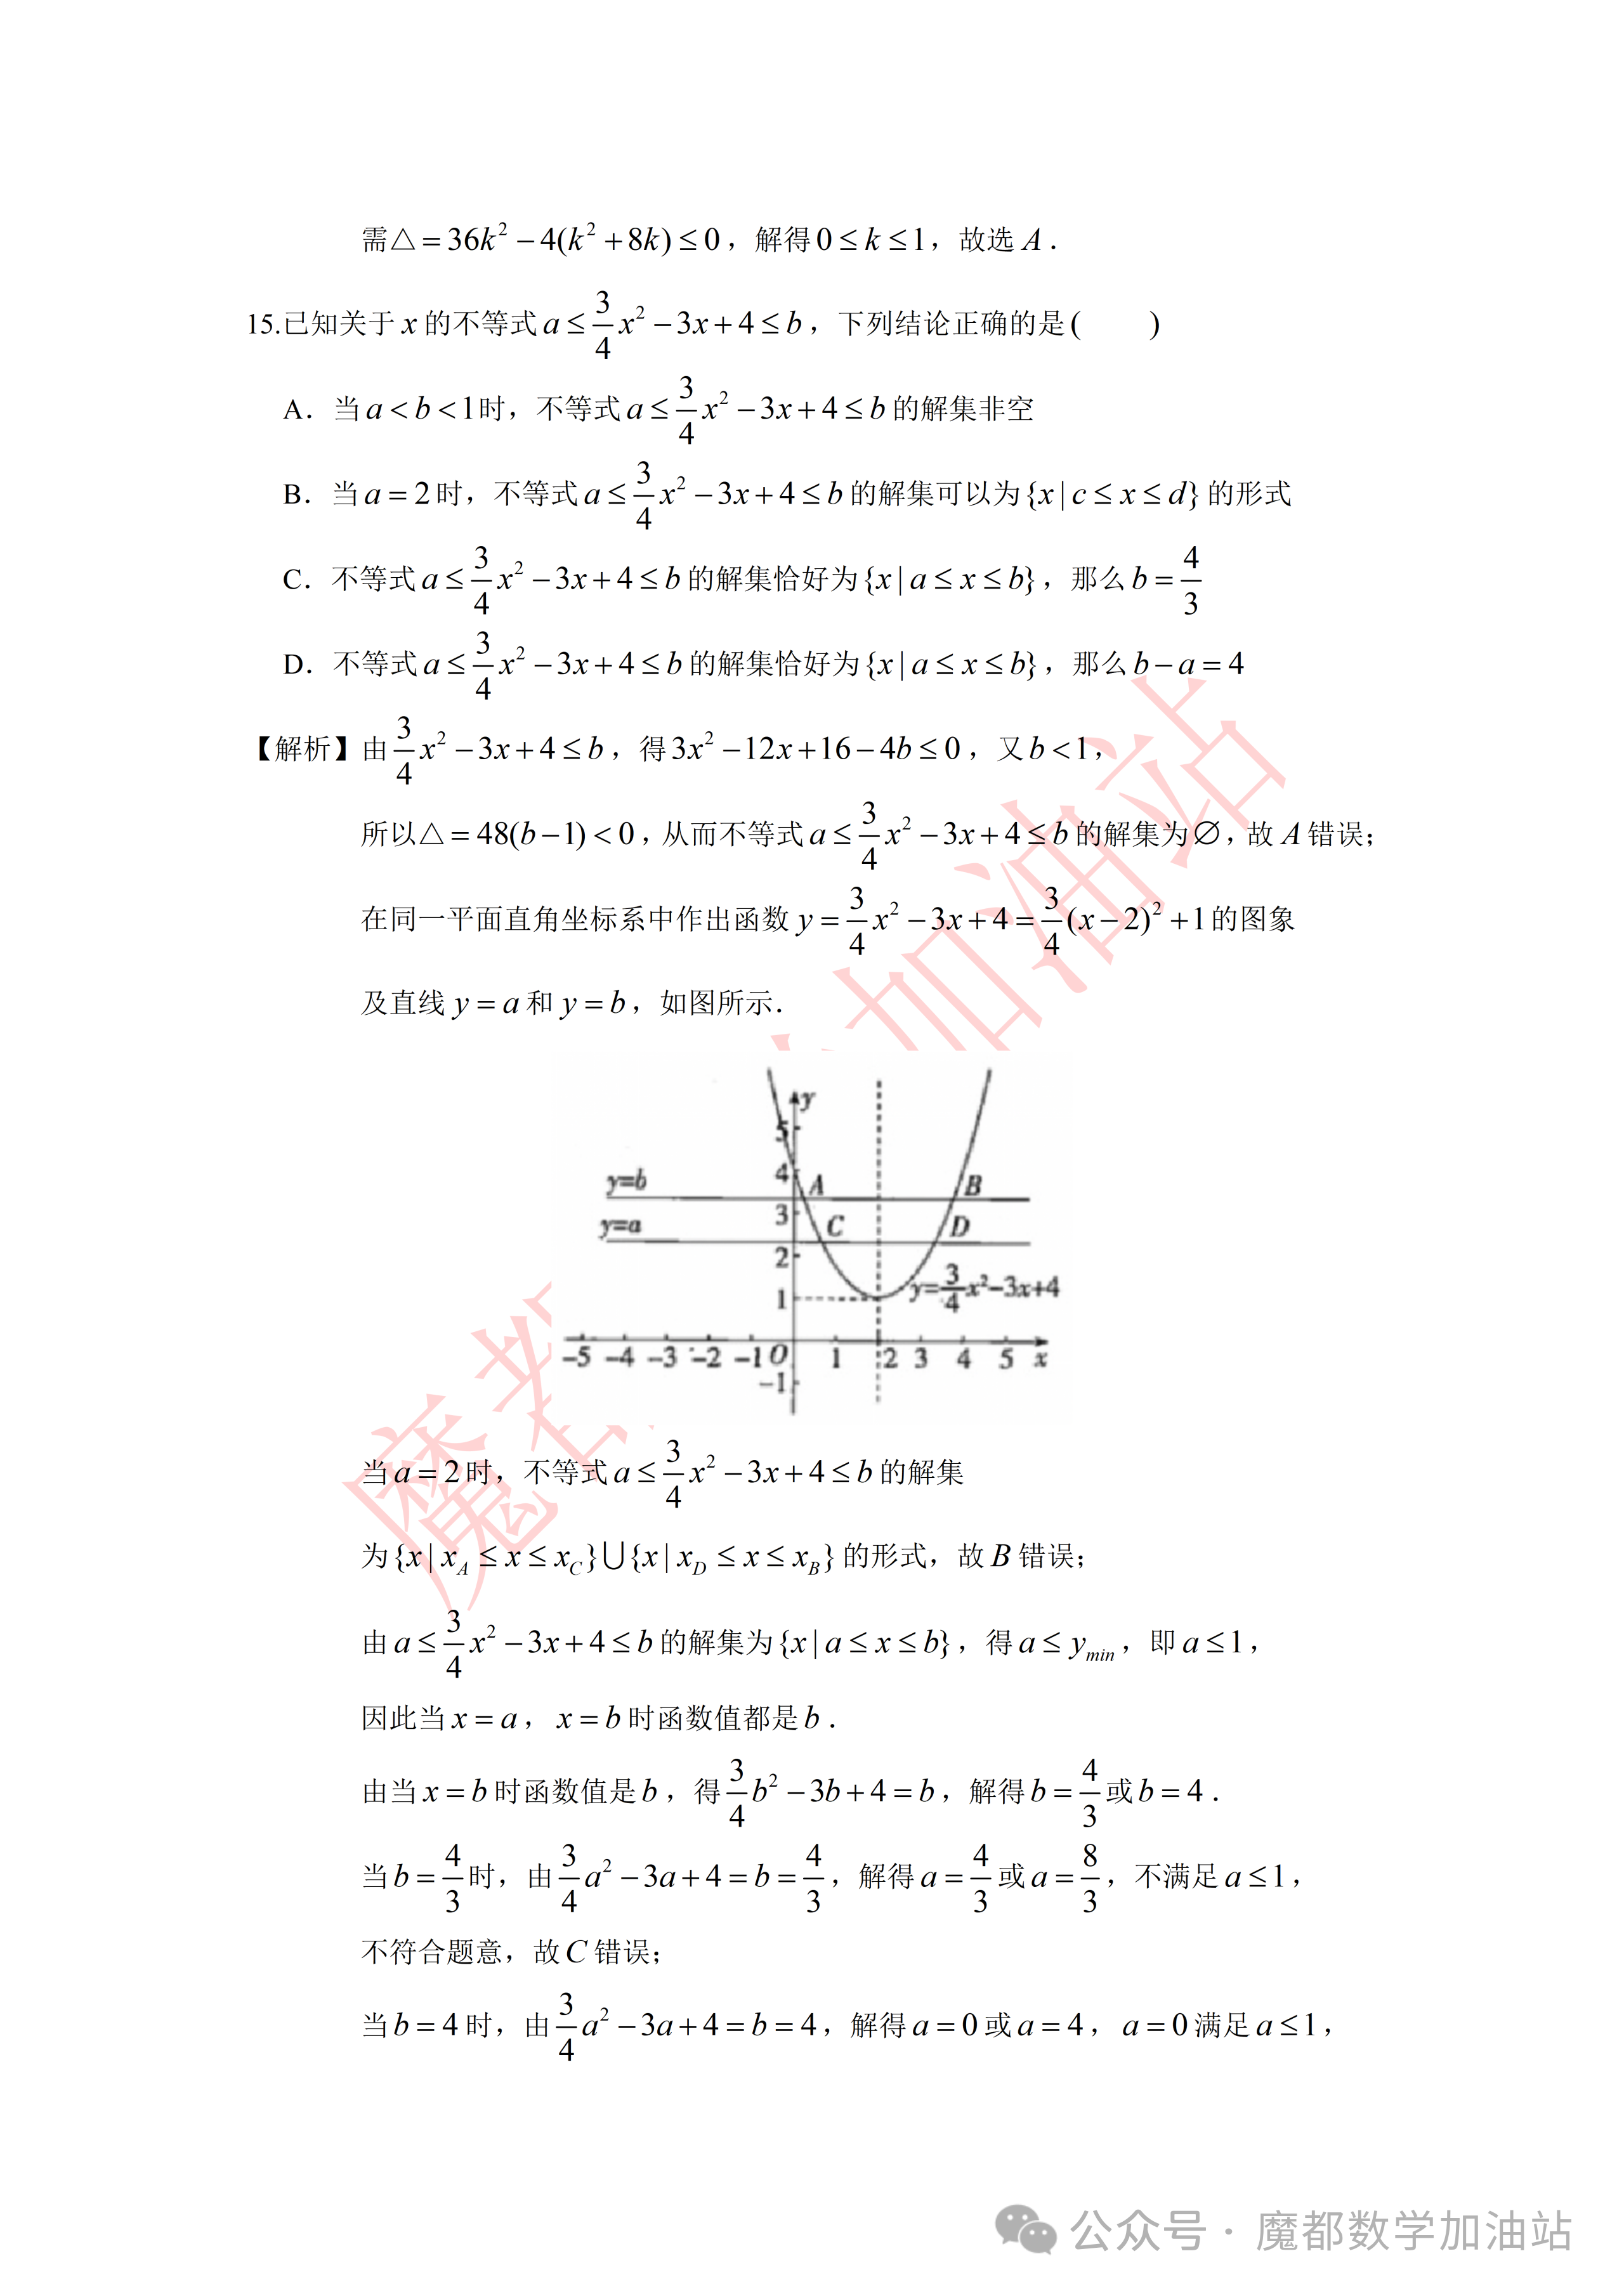
\includegraphics[width=.55\linewidth,trim=900bp 1400bp 760bp 1680bp,clip]{../原图/高一46_交附闵行_国庆作业3/05.png}
\end{center}
\step{当 $a=2$ 时，不等式 $a\leqslant\dfrac34x^2-3x+4\leqslant b$ 的解集为
$\{x\mid x_A\leqslant x\leqslant x_C\}\cup\{x\mid x_D\leqslant x\leqslant x_B\}$ 的形式，故 $B$ 错误；}
\step{由 $a\leqslant\dfrac34x^2-3x+4\leqslant b$ 的解集恰好为 $\{x\mid a\leqslant x\leqslant b\}$ 的形式，得 $a\leqslant y_{\min}$，即 $a\leqslant1$，}
\step{因为当 $x=a$、$x=b$ 时函数值都是 $b$，当 $x=a$ 时，$\dfrac34a^2-3a+4=b$；当 $x=b$ 时，$\dfrac34b^2-3b+4=b$，}
\step{解得 $b=\dfrac43$ 或 $b=4$，}
\step{当 $b=\dfrac43$ 时，由 $\dfrac34a^2-3a+4=b$，解得 $a=\dfrac43$ 或 $a=\dfrac83$，不符合题意，故 $C$ 错误；}
\step{当 $b=4$ 时，由 $\dfrac34a^2-3a+4=b$，解得 $a=0$ 或 $a=4$，$a=0$ 满足 $a\leqslant1$，故 $D$ 正确；}
\step{故选 $D$.}
\solend
\fi

\item 已知 $x$、$y\in(0,+\infty)$，则 $(x-y)^2+2y+1-x+\dfrac4x$ 的最小值为\mbox{（\quad）}

\keepwithprev
A. $1$\qquad B. $2$\qquad C. $3$\qquad D. $4$

\ans{$D$}

\ifanswer
\solbegin
\step{因为 $(x-y)^2+2y+1-x+\dfrac4x=(x-y-1)^2+x+\dfrac4x$，}
\step{当且仅当 $x-y-1=0$，且 $x=\dfrac4x$ 时取等号，}
\step{又因为 $x+\dfrac4x\geqslant2\sqrt{x\cdot\dfrac4x}=4$，当且仅当 $x=2$ 时取等号，}
\step{故选 $D$.}
\solend
\fi

\end{enumerate}

\bigsec{三、解答题}

\begin{enumerate}
\setcounter{enumi}{16}

\item 设集合 $A=\left\{x\middle|\dfrac{x-3}{x-1}<0\right\}$，$B=\{x\mid x^2-2ax+a^2-1>0\}$.
\begin{enumerate}[label=(\arabic*)]
\item 若 $a=3$，求 $A\cup B$；
\item 若“$x\in A$”是“$x\in B$”的充分条件，求实数 $a$ 的取值范围.
\end{enumerate}

\ifanswer
\solbegin
% 注：原卷题干为 a^2-1，故 a=3 时常数项为 8；题干与本步一致。
\stepm{(1)}{当 $a=3$ 时，$B=\{x\mid x^2-6x+8>0\}=\{x\mid x<2\text{ 或 }x>4\}$；}
\step{因为 $A=\left\{x\middle|\dfrac{x-3}{x-1}<0\right\}=\{x\mid(x-1)(x-3)<0\}=\{x\mid1<x<3\}$，}
\step{所以 $A\cup B=\{x\mid x<2\text{ 或 }x>4\}\cup\{x\mid1<x<3\}
=\{x\mid x<3\text{ 或 }x>4\}$.}
\stepm{(2)}{因为“$x\in A$”是“$x\in B$”的充分条件，所以 $A\subseteq B$，}
\step{因 $A=\left\{x\middle|\dfrac{x-3}{x-1}<0\right\}
=\{x\mid(x-1)(x-3)<0\}=\{x\mid1<x<3\}$，}
\step{所以 $A\subseteq B=\{x\mid x<a-1\text{ 或 }x>a+1\}$，}
\step{要使 $A\subseteq B$，需有 $a-1\geqslant3$ 或 $a+1\leqslant1$，}
\step{所以 $a\geqslant4$ 或 $a\leqslant0$，故 $a$ 的取值范围为 $\{a\mid a\geqslant4\text{ 或 }a\leqslant0\}$.}
\solend
\fi

\ansspace[6]

\item 某学校引入种植类劳动教育课程，打算围成如图所示的四块全等的长方形田地种植不同种类的蔬菜，其中一面可以利用原有的墙（足够长），其他各面需要用篱笆围成，设其中一块田地为矩形 $ABCD$.

\begin{center}
% 原图第 6 页配图直接裁取。
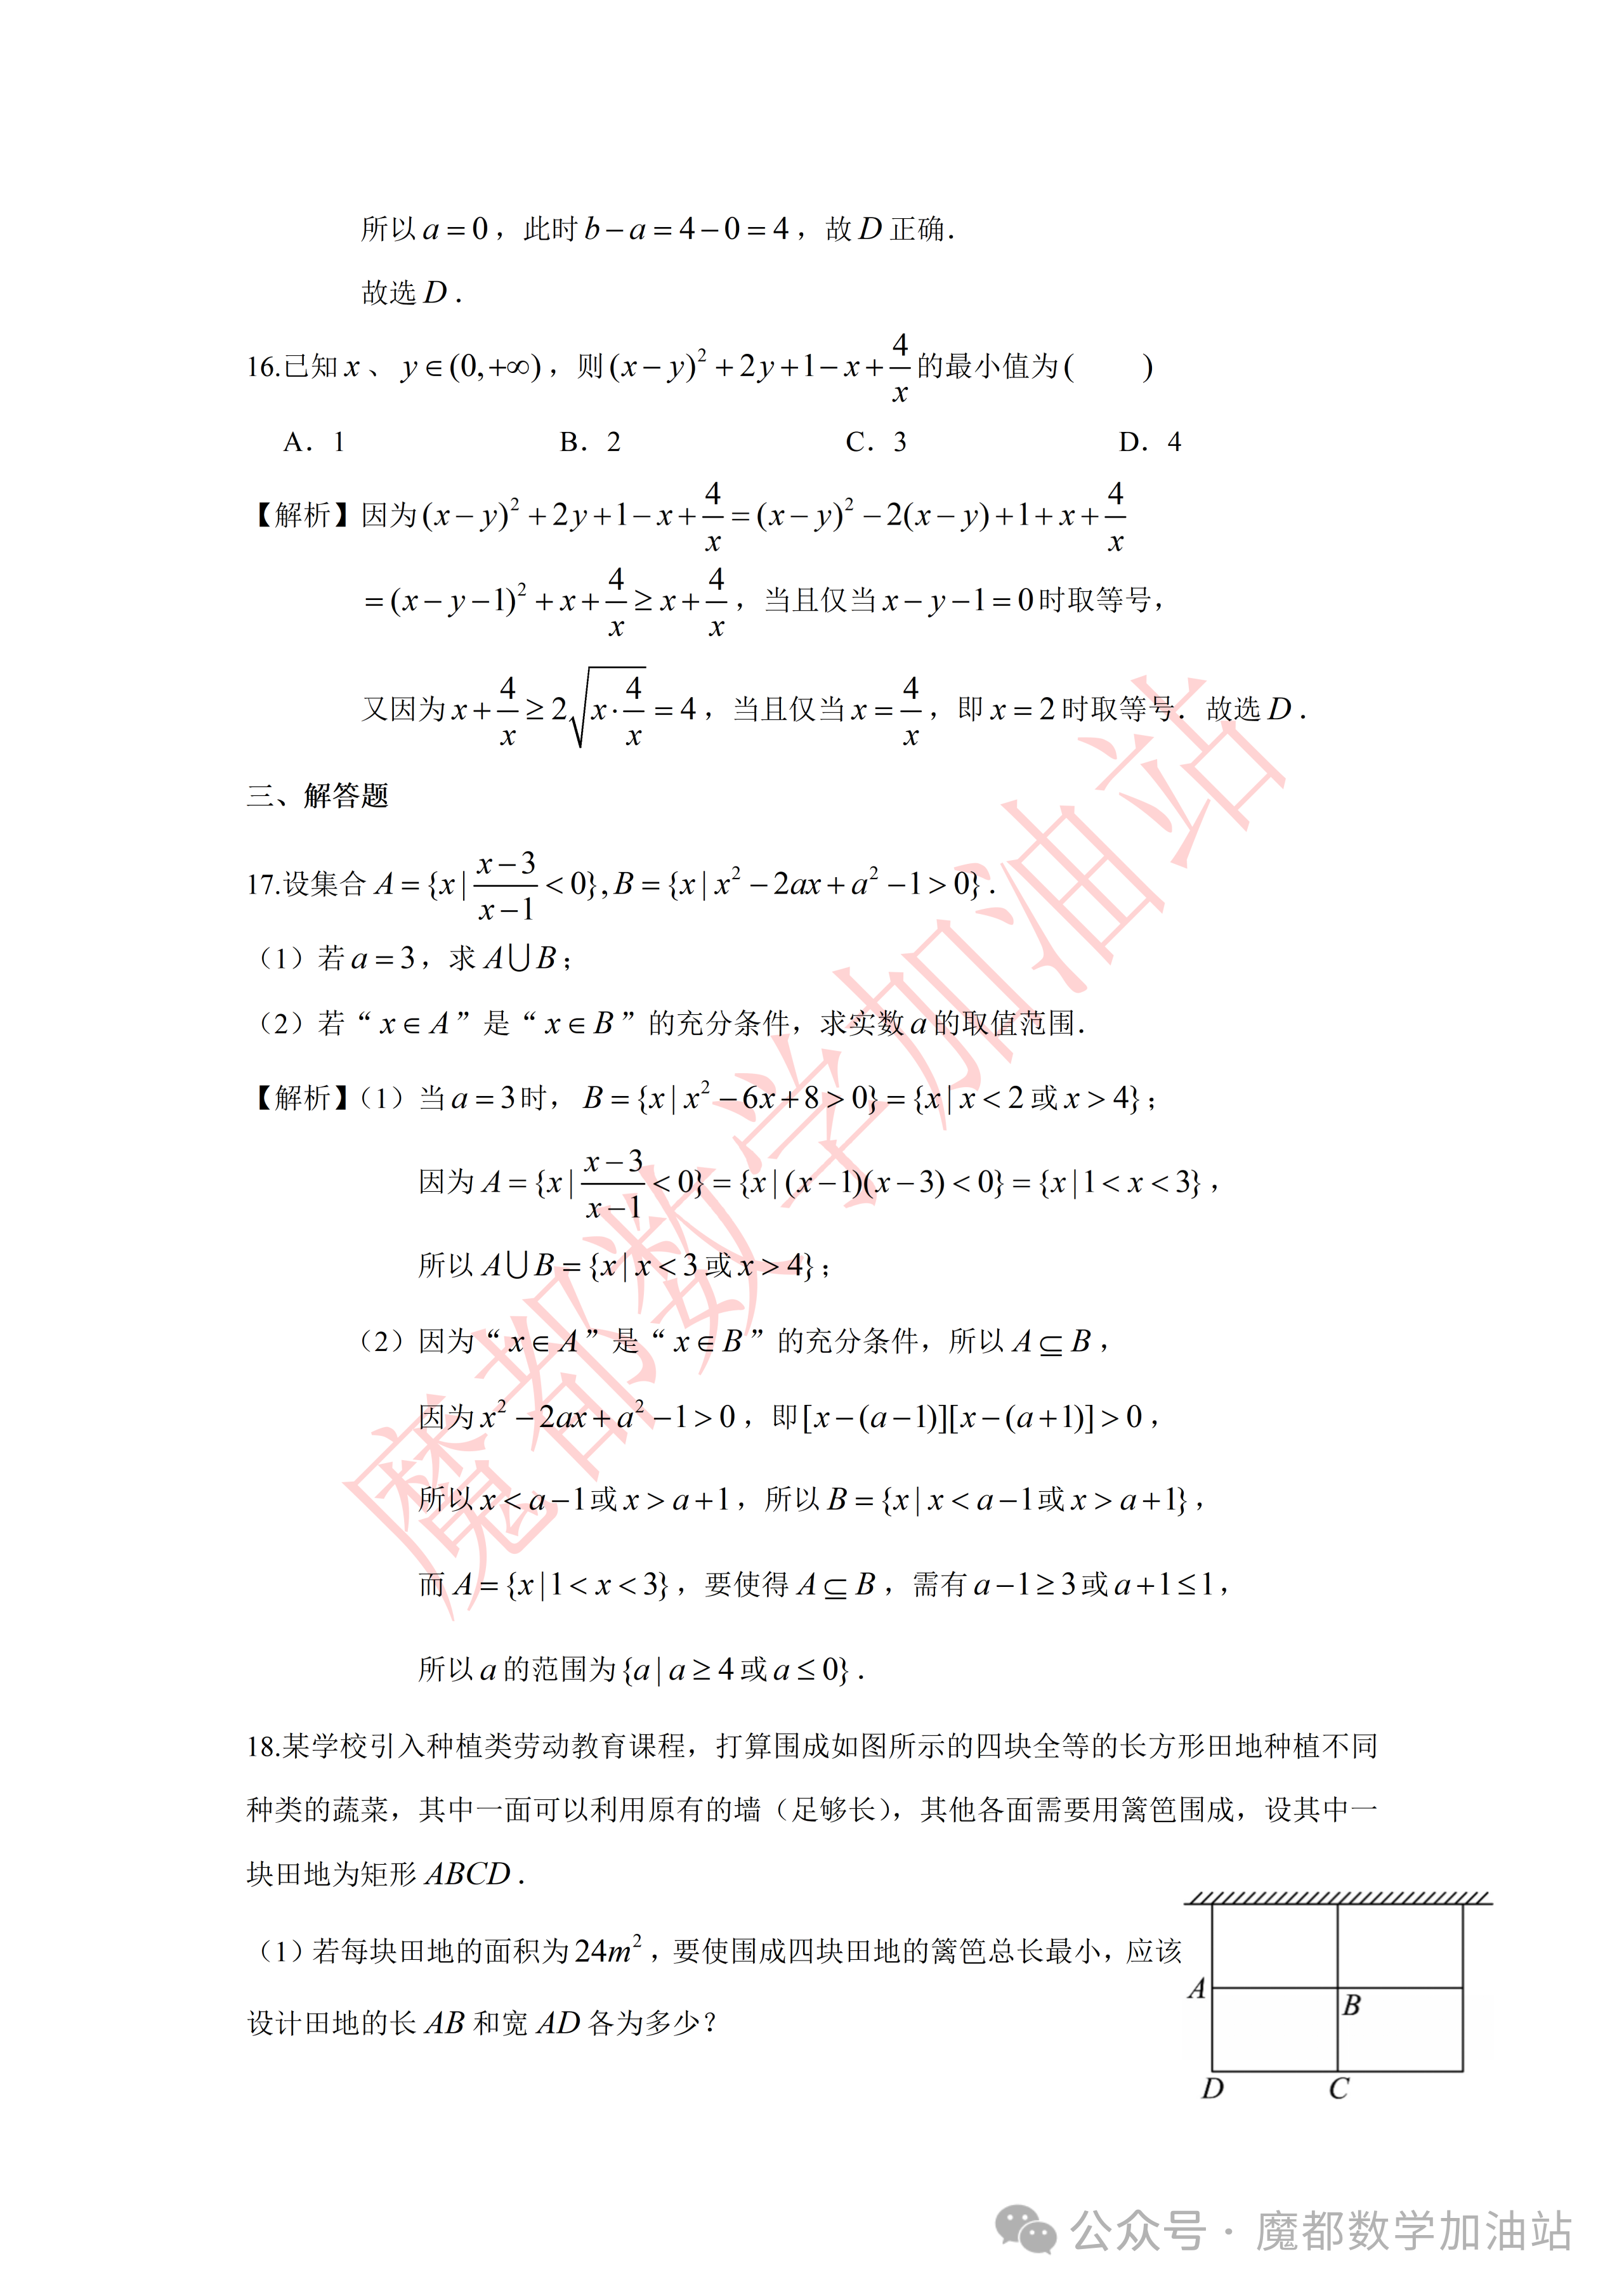
\includegraphics[width=.33\linewidth,trim=1866bp 220bp 210bp 2960bp,clip]{../原图/高一46_交附闵行_国庆作业3/06.png}
\end{center}

\begin{enumerate}[label=(\arabic*)]
\item 若每块田地的面积为 $24\,\text{m}^2$，要使围成四块田地的篱笆总长最小，应该设计田地的长 $AB$ 和宽 $AD$ 各为多少？
\item 现有 $40\,\text{m}$ 长的篱笆，要使每块田地的面积最大，应该设计田地的长 $AB$ 和宽 $AD$ 各为多少？
\end{enumerate}

\ifanswer
\solbegin
\stepm{(1)}{设 $AB$ 长为 $x\,\text{m}$，$AD$ 宽为 $y\,\text{m}$，由题意得 $xy=24$，篱笆总长为 $4x+6y$，}
\step{$4x+6y\geqslant2\sqrt{4x\cdot6y}=2\sqrt{24xy}=48$，}
\step{当且仅当 $4x=6y$ 时取等号，解得 $x=6$，$y=4$，}
\step{所以田地的长 $AB$ 为 $6\,\text{m}$，宽 $AD$ 为 $4\,\text{m}$.}
\stepm{(2)}{设 $AB$ 长为 $a\,\text{m}$，$AD$ 宽为 $b\,\text{m}$，由篱笆总长 $4a+6b=40$，即 $2a+3b=20$，}
\step{将 $a=\dfrac{20-3b}{2}$ 代入每块田地面积 $ab$，得 $ab=\dfrac12b(20-3b)=-\dfrac32b^2+10b$，}
\step{当 $b=\dfrac{10}{3}$ 时，$ab$ 最大，此时 $a=5$，}
\step{所以田地的长 $AB$ 为 $5\,\text{m}$，宽 $AD$ 为 $\dfrac{10}{3}\,\text{m}$.}
\solend
\fi

\ansspace[8]

\item 已知 $x_1$、$x_2$ 是一元二次方程 $4kx^2-4kx+k+1=0$ 的两个不等实数根.
\begin{enumerate}[label=(\arabic*)]
\item 若 $x_1$、$x_2$ 均为正根，求实数 $k$ 的取值范围；
\item 求使 $\dfrac{x_1}{x_2}+\dfrac{x_2}{x_1}-2$ 的值为整数 $k$ 的整数值.
\end{enumerate}

\ifanswer
\solbegin
\stepm{(1)}{由题意，$x_1$、$x_2$ 是方程 $4kx^2-4kx+k+1=0$ 的两个不等实数根，}
\step{故 $k\neq0$，$\Delta=(-4k)^2-16k(k+1)>0$，得 $-16k>0$，所以 $k<0$，}
\step{又 $x_1+x_2=1$，$x_1x_2=\dfrac{k+1}{4k}>0$，得 $k+1<0$，}
\step{所以 $k$ 的取值范围为 $(-\infty,-1)$.}
\stepm{(2)}{由题意，}
\step{$\dfrac{x_1}{x_2}+\dfrac{x_2}{x_1}-2
=\dfrac{x_1^2+x_2^2-2x_1x_2}{x_1x_2}
=\dfrac{(x_1+x_2)^2-4x_1x_2}{x_1x_2}$，}
\step{又 $x_1+x_2=1$，$x_1x_2=\dfrac{k+1}{4k}$，}
\step{则 $\dfrac{x_1}{x_2}+\dfrac{x_2}{x_1}-2=-\dfrac4{k+1}$，}
\step{由于 $-\dfrac4{k+1}$ 为整数，故 $k+1$ 只能取 $\pm1$、$\pm2$、$\pm4$，又 $k<-1$，}
\step{所以整数 $k$ 的值为 $-2$、$-3$、$-5$.}
\solend
\fi

\ansspace[8]

\item 已知 $a>0$，$b>0$，且 $2a+3b=3$.
\begin{enumerate}[label=(\arabic*)]
\item 求 $ab$ 的最大值；
\item 求 $a-\dfrac1{6b}$ 的最大值；
\item 求 $\dfrac2a+\dfrac3{b+1}$ 的最小值.
\end{enumerate}

\ifanswer
\solbegin
\stepm{(1)}{由 $2a+3b=3$，得 $3=2a+3b\geqslant2\sqrt{6ab}$，}
\step{所以 $ab\leqslant\dfrac38$，当且仅当 $2a=3b=\dfrac32$ 时取等号，}
\step{故 $ab$ 的最大值为 $\dfrac38$.}
\stepm{(2)}{由 $2a+3b=3$，得 $a=\dfrac32-\dfrac32b$，}
\step{则 $a-\dfrac1{6b}=\dfrac32-\dfrac32b-\dfrac1{6b}$，}
\step{由基本不等式，$\dfrac32b+\dfrac1{6b}\geqslant2\sqrt{\dfrac32b\cdot\dfrac1{6b}}=1$，}
\step{当且仅当 $\dfrac32b=\dfrac1{6b}$，即 $b=\dfrac13$、$a=1$ 时取等号，}
\step{所以 $a-\dfrac1{6b}$ 的最大值为 $\dfrac12$.}
\stepm{(3)}{由 $2a+3b=3$，得 $2a+3(b+1)=6$，}
\step{$\dfrac2a+\dfrac3{b+1}
=\dfrac16\left(2a+3(b+1)\right)\left(\dfrac2a+\dfrac3{b+1}\right)$}
\step{$=\dfrac16\left(13+\dfrac{6(b+1)}a+\dfrac{6a}{b+1}\right)
\geqslant\dfrac16\left(13+2\sqrt{\dfrac{6(b+1)}a\cdot\dfrac{6a}{b+1}}\right)=\dfrac{25}{6}$，}
\step{当且仅当 $a=b+1$，即 $a=\dfrac65$、$b=\dfrac15$ 时取等号，}
\step{所以 $\dfrac2a+\dfrac3{b+1}$ 的最小值为 $\dfrac{25}{6}$.}
\solend
\fi

\ansspace[8]

\item 已知 $U=\R$ 为全集，集合 $A=\{s^2+3t^2\mid s,t\in U\}$.
\begin{enumerate}[label=(\arabic*)]
\item 设 $U=\{1,3,5\}$，求集合 $A$ 的元素个数；
\item 设 $U=\Z$，证明：若 $x\in A$，则 $7x\in A$；
\item 设 $U=\R$，$x$、$y\in A$，且 $x=m^2+3n^2$，$y=p^2+3q^2$，若 $mp-3nq=\sqrt3$，求 $x+y+mq+np$ 的最小值.
\end{enumerate}

\ifanswer
\solbegin
\stepm{(1)}{当 $s=1$，$t=1$ 时，$s^2+3t^2=1+3=4$；}
\step{当 $s=1$，$t=3$ 时，$s^2+3t^2=1+27=28$；}
\step{当 $s=1$，$t=5$ 时，$s^2+3t^2=1+75=76$；}
\step{当 $s=3$，$t=1$ 时，$s^2+3t^2=9+3=12$；}
\step{当 $s=3$，$t=3$ 时，$s^2+3t^2=9+27=36$；}
\step{当 $s=3$，$t=5$ 时，$s^2+3t^2=9+75=84$；}
\step{当 $s=5$，$t=1$ 时，$s^2+3t^2=25+3=28$；}
\step{当 $s=5$，$t=3$ 时，$s^2+3t^2=25+27=52$；}
\step{当 $s=5$，$t=5$ 时，$s^2+3t^2=25+75=100$，}
\step{所以 $A=\{4,12,28,36,52,76,84,100\}$，有 $8$ 个元素.}
\stepm{(2)}{因为 $U=\Z$，$x\in A$，设 $x=s^2+3t^2$，}
\step{则 $7x=7(s^2+3t^2)=(2s+3t)^2+3(s-2t)^2\in A$，}
\step{所以 $7x\in A$.}
\stepm{(3)}{因为 $x=m^2+3n^2$，$y=p^2+3q^2$，}
\step{$xy=(m^2+3n^2)(p^2+3q^2)=3(mq+np)^2+(mp-3nq)^2$，}
\step{设 $mq+np=b$，则 $xy=3b^2+3$，所以 $y=\dfrac{3b^2+3}{x}$，}
\step{于是 $x+y+mq+np=x+\dfrac{3b^2+3}{x}+b\geqslant2\sqrt{3b^2+3}+b$，}
\step{设 $2\sqrt{3b^2+3}+b=t$，整理得 $11b^2+2bt+12-t^2=0$，}
\step{判别式法，$\Delta=4t^2-44(12-t^2)\geqslant0$，得 $t\geqslant\sqrt{11}$，}
\step{即 $(x+y+mq+np)_{\min}=\sqrt{11}$，所以 $x+y+mq+np$ 的最小值为 $\sqrt{11}$.}
\solend
\fi

\ansspace*[10]

\end{enumerate}

\end{document}
"
% 紧凑版：xelatex "\def\iscompact{1}% 高一46_交附闵行_国庆作业3.tex
%   —— 高一上数学“2026-2027 年交附闵行高一上国庆作业 3”（讲评版）
% 试卷版：xelatex 高一46_交附闵行_国庆作业3.tex
% 答案版：xelatex "\def\isanswer{1}% 高一46_交附闵行_国庆作业3.tex
%   —— 高一上数学“2026-2027 年交附闵行高一上国庆作业 3”（讲评版）
% 试卷版：xelatex 高一46_交附闵行_国庆作业3.tex
% 答案版：xelatex "\def\isanswer{1}\input{高一46_交附闵行_国庆作业3.tex}"
% 紧凑版：xelatex "\def\iscompact{1}\input{高一46_交附闵行_国庆作业3.tex}"
%
% 原始材料：微信公众号“魔都数学加油站”，作者破晓，2026-10-02 17:56 发布。
% 原文标题：“27学年高一46——2026-2027你那上海市交附闵行高一上国庆作业3”
% （公众号标题中的“你那”照录，系原文标题字样）；原文链接：
% http://mp.weixin.qq.com/s?__biz=Mzg4ODU1ODMxOQ==&mid=2247591657&idx=3&sn=a894d1a16611283a61b3eaba32a3f24c&chksm=cee83366c6a55381b370069f84ef63d20251f94608bb37cc4ec2d66227401bd147f4f6bd8256&scene=126&sessionid=1790935402&subscene=7&clicktime=1790937618&enterid=1790937618#rd
% 正文为 9 张 PNG 页，按页序读取原图；第 01、02、07 页 4762×6735，
% 第 03—06、08、09 页 2560×3620。卷面标题照原卷印作“2026-2027 年交附闵行高一上国庆作业 3”。
% 原文从第 3 题起，题号照原卷保留；正文为讲评版，答案、解析依原卷顺序录入。
% 水印及页脚公众号标识不录入。卷面插图直接裁取对应原图页，不另制图片文件。
%
% 与原卷的排版差异：
%   ① 原卷按“一、填空题”“二、选择题”“三、解答题”分节，本稿沿用原节与原题号，
%      只改排为全稿统一的大节样式；
%   ② 原卷答案与解析依页面位置分布，本稿按 common.sty 统一置于答案版；
%   ③ 原卷副标题未印，本稿按“知识模块”口径标作“集合与常用逻辑用语、不等式”。
%
% 原卷存疑一处（照抄未改，见第 12 题题干及解析处注释）：
%   第 12 题题干同时给出 x∈Z，却称不等式组有“50 个不等的实数解”；解析按整数根计数。
%   此处题干与解析的原文不一致，本稿均照录。
% 第 17 题曾疑似有常数项不一致：复核原图题干为 a^2-1，a=3 时常数项确为 8，
% 与解析相符；不将其记作原卷错误。
%
\documentclass[a4paper,11pt]{article}
\usepackage{common}

\begin{document}

\examtitlest[3]{2026--2027 年交附闵行高一上国庆作业 3}{集合与常用逻辑用语、不等式}

\bigsec{一、填空题}

\begin{enumerate}
\setcounter{enumi}{2}

\item 不等式 $\dfrac{x^2-10}{x+2}\geqslant1$ 的解集为\blankline[4.4em].

\ifanswer
\ans{$\{x\mid-3\leqslant x<-2\text{ 或 }x\geqslant4\}$}
\solbegin
\step{不等式 $\dfrac{x^2-10}{x+2}\geqslant1$，移项得 $\dfrac{x^2-10}{x+2}-1\geqslant0$，}
\step{通分得 $\dfrac{x^2-x-12}{x+2}\geqslant0$，即 $\dfrac{(x-4)(x+3)}{x+2}\geqslant0$，}
\step{解得 $-3\leqslant x<-2$ 或 $x\geqslant4$，}
\step{故不等式的解集为 $\{x\mid-3\leqslant x<-2\text{ 或 }x\geqslant4\}$.}
\solend
\fi

\item $|x-3|+|x-5|\geqslant2$，当等号成立时，$x$ 的范围是\blankline[4.4em].

\ifanswer
\ans{$[3,5]$}
\fi

\item 若直角三角形斜边长等于 $4\sqrt2\,\text{cm}$，则直角三角形面积的最大值为\blankline[4.4em].

\ifanswer
\solbegin
\step{设 $Rt\triangle ABC$ 中，$C=90^\circ$，则 $c=\sqrt{a^2+b^2}=4\sqrt2$，所以 $a^2+b^2=32$，}
\step{由基本不等式得 $a^2+b^2\geqslant2ab$，当且仅当 $a=b=4$ 时取等号，}
\step{所以 $\triangle ABC$ 的面积 $S=\dfrac12ab\leqslant8$，}
\step{当且仅当 $a=b=4$ 时，$\triangle ABC$ 的面积最大值为 $8$.}
\solend
\fi

\item 不等式 $(x-1)(2-x)>0$ 的解集为\blankline[4.4em].

\ifanswer
\solbegin
\step{$(x-1)(2-x)>0\Rightarrow(x-1)(x-2)<0$，}
\step{故不等式的解集为 $\{x\mid1<x<2\}$.}
\solend
\fi

\item 已知集合 $A=\{1,2\}$，$B=\{x\mid x^2-2mx+m=0\}$，$A\cup B=A$，则实数 $m$ 的取值范围为\blankline[4.4em].

\ifanswer
\solbegin
\step{因为 $A\cup B=A$，所以 $B\subseteq A$，}
\step{当 $B=\varnothing$ 时，$\Delta=(-2m)^2-4m<0$，解得 $0<m<1$，}
\step{当 $B$ 为单元素集时，$\Delta=0$，解得 $m=0$ 或 $m=1$，}
\step{当 $m=0$ 时，方程 $x^2=0$，解得 $x=0$，此时 $B=\{0\}$，不满足 $B\subseteq A$；}
\step{当 $m=1$ 时，方程 $x^2-2x+1=0$，解得 $x=1$，此时 $B=\{1\}$，满足 $B\subseteq A$；}
\step{当 $B=\{1,2\}$ 时，由韦达定理得 $1+2=2m$，$1\times2=m$，无解，}
\step{综上所述，实数 $m$ 的取值范围为 $\{m\mid0<m\leqslant1\}$.}
\solend
\fi

\item 设 $a$、$b$、$c\in\R^+$，若 $a+b+c=1$，则 $\dfrac1a+\dfrac1b+\dfrac1c\geqslant$\blankline[4.4em].

\ifanswer
\solbegin
\step{因为 $a$、$b$、$c\in\R^+$，且 $a+b+c=1$，}
\step{所以 $\dfrac1a+\dfrac1b+\dfrac1c=(a+b+c)\left(\dfrac1a+\dfrac1b+\dfrac1c\right)$}
\step{$=3+\dfrac ab+\dfrac ba+\dfrac ac+\dfrac ca+\dfrac bc+\dfrac cb$，}
\step{由基本不等式得 $\dfrac ab+\dfrac ba\geqslant2$，$\dfrac ac+\dfrac ca\geqslant2$，$\dfrac bc+\dfrac cb\geqslant2$，}
\step{所以 $\dfrac1a+\dfrac1b+\dfrac1c\geqslant9$，当且仅当 $a=b=c=\dfrac13$ 时取等号，}
\step{所以 $\dfrac1a+\dfrac1b+\dfrac1c$ 的最小值为 $9$.}
\solend
\fi

\item 已知 $-1\leqslant x+y\leqslant2$，$-2\leqslant x-y\leqslant1$，则 $x-2y$ 的范围为\blankline[4.4em].

\ifanswer
\solbegin
\step{设 $x-2y=m(x+y)+n(x-y)$，}
\step{则 $x-2y=(m+n)x+(m-n)y$，所以 $m+n=1$，$m-n=-2$，}
\step{解得 $m=-\dfrac12$，$n=\dfrac32$，}
\step{所以 $x-2y=-\dfrac12(x+y)+\dfrac32(x-y)$，}
\step{因为 $-1\leqslant x+y\leqslant2$，$-2\leqslant x-y\leqslant1$，}
\step{所以 $-4\leqslant x-2y\leqslant2$，即 $x-2y$ 的范围为 $[-4,2]$.}
\solend
\fi

\item 设集合 $A=\{1,2,m\}$，其中 $m$ 为实数，令 $B=\{a^2\mid a\in A\}$，$C=A\cup B$. 若 $C$ 中所有元素之和为 $6$，则 $C$ 中的所有元素之积为\blankline[4.4em].

\ifanswer
\solbegin
\step{因为 $A=\{1,2,m\}$，所以 $B=\{a^2\mid a\in A\}=\{1,4,m^2\}$，$m\neq1$，$m\neq2$，}
\step{又 $C=A\cup B$，所以 $1\in C$，$4\in C$，$m^2\in C$，}
\step{若 $m^2=1$，则 $m=-1$ 或 $m=1$（舍），当 $m=-1$ 时，$C=\{1,2,4,-1\}$，$C$ 中所有元素之和为 $6$，}
\step{此时 $C$ 中所有元素之积为 $-8$；}
\step{若 $m^2=2$，则 $m=-\sqrt2$ 或 $m=\sqrt2$，$C$ 中所有元素之和不符合题意；}
\step{若 $m^2=4$，则 $m=-2$ 或 $m=2$，此时 $C=\{1,2,4,-2\}$ 或 $C=\{1,2,4\}$，所有元素之和不符合题意；}
\step{若 $m^2\neq1$，$m^2\neq2$，$m^2\neq4$，则 $C=\{1,2,4,m,m^2\}$，}
\step{所以 $1+2+4+m+m^2=6$，即 $m^2+m+1=0$，无解，}
\step{综上所述，$C$ 中所有元素之积为 $-8$.}
\solend
\fi

\item 若对任意实数 $x>0$，$y>0$，不等式 $x+\sqrt{xy}\leqslant a(x+y)$ 恒成立，则实数 $a$ 的最小值为\blankline[4.4em].

\ifanswer
\solbegin
\step{由不等式 $x+\sqrt{xy}\leqslant a(x+y)$ 对任意实数 $x>0$，$y>0$ 恒成立，}
\step{得 $a\geqslant\dfrac{x+\sqrt{xy}}{x+y}$，}
\step{设 $\sqrt{\dfrac yx}=t>0$，则 $a\geqslant\dfrac{1+t}{1+t^2}$，}
\step{$\dfrac{1+t}{1+t^2}\leqslant\dfrac{\sqrt2+1}{2}$，当且仅当 $t=\sqrt2-1$ 时取等号，}
\step{所以实数 $a$ 的最小值为 $\dfrac{\sqrt2+1}{2}$.}
\solend
\fi

% 注：原卷题干给出 x∈Z，却写“实数解”；解析按整数解计数，题干与解析不一致，照录未改。
\item 若关于 $x$ 的不等式组
$\begin{cases}x^2-3mx\geqslant4m^2\\-20<x<120\end{cases}$（$x\in\Z,m>0$）恰有 $50$ 个不等的实数解，则 $m$ 的取值范围为\blankline[4.4em]（结果用区间表示）.

\ifanswer
\solbegin
\step{由 $x^2-3mx\geqslant4m^2$ 以及 $m>0$，解得 $x\leqslant-m$ 或 $x\geqslant4m$，}
\step{由原不等式组恰有 $50$ 个不等的实数解，可画出如下解集区间：}
\begin{center}
% 原图第 4 页数轴图直接裁取。
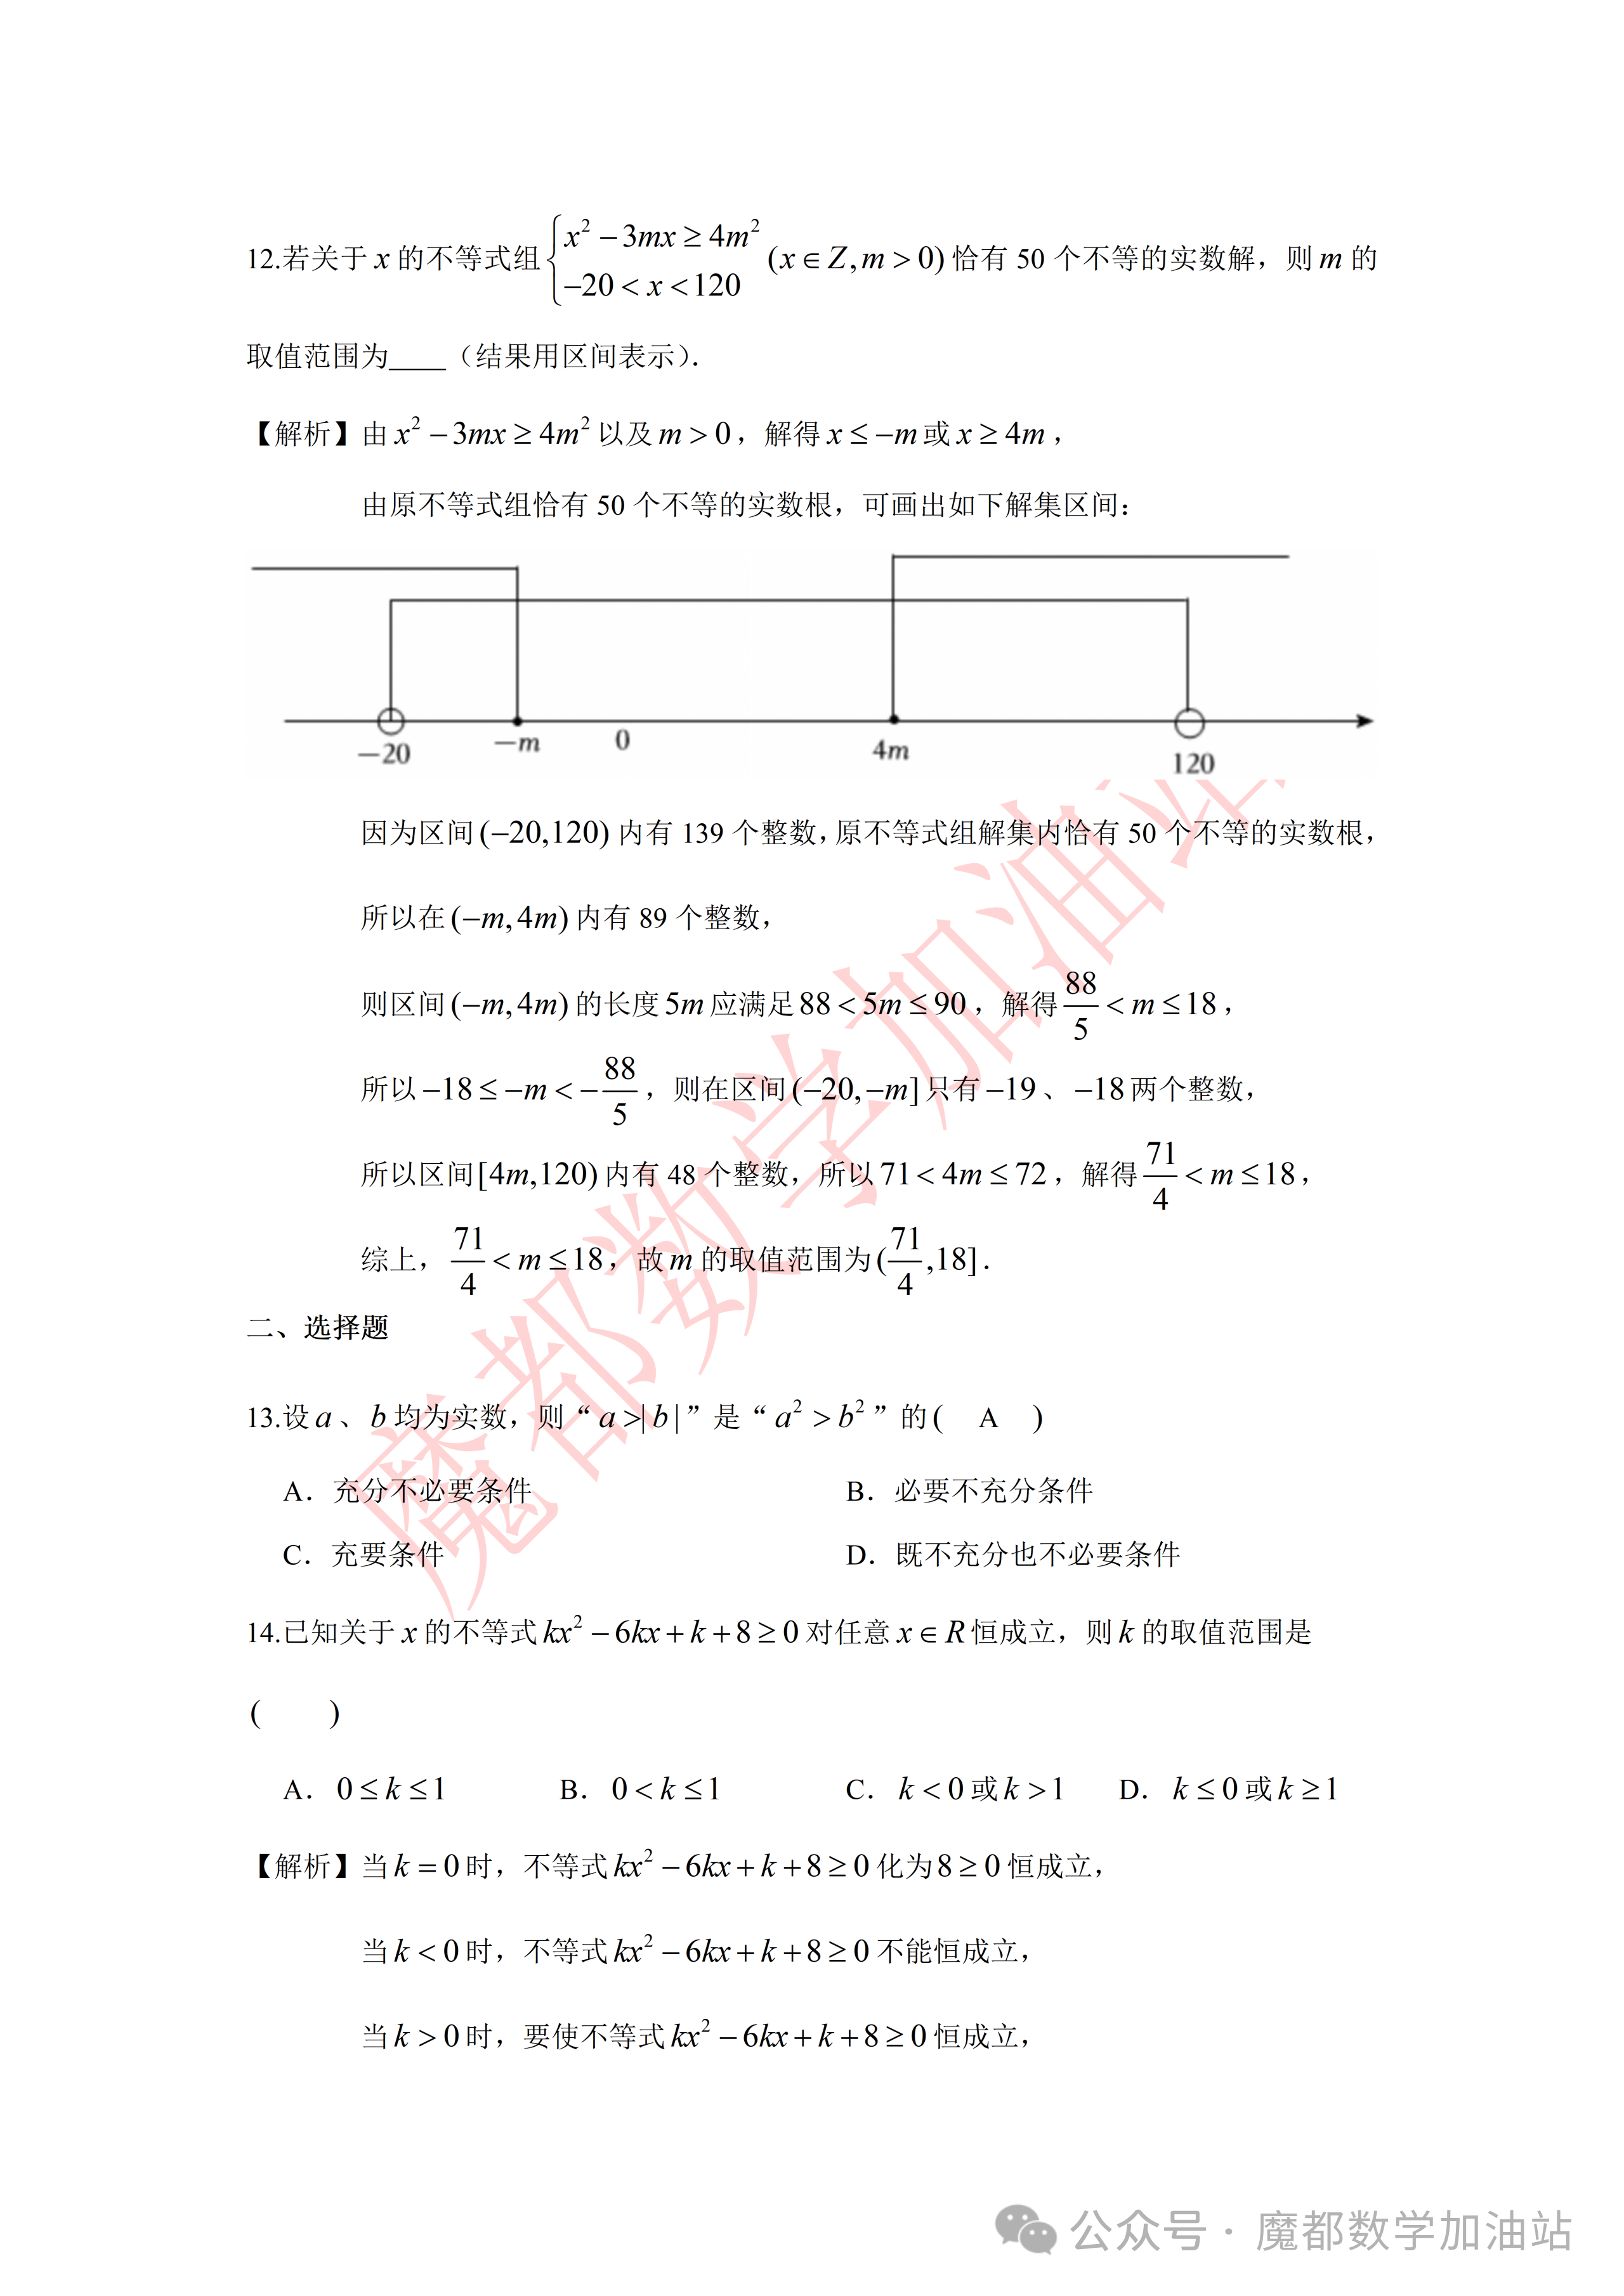
\includegraphics[width=.88\linewidth,trim=400bp 2410bp 320bp 860bp,clip]{../原图/高一46_交附闵行_国庆作业3/04.png}
\end{center}
\step{因为区间 $(-20,120)$ 内有 $139$ 个整数，原不等式组解集内有 $50$ 个不等的整数根，}
\step{所以在区间 $(-m,4m)$ 内有 $89$ 个整数，}
\step{则区间 $(-m,4m)$ 的长度 $5m$ 应满足 $88<5m\leqslant90$，解得 $\dfrac{88}{5}<m\leqslant18$，}
% 注：原卷题干称“实数解”，本行及后文按原卷解析照录为整数根计数。
\step{所以 $-18\leqslant-m<-\dfrac{88}{5}$，则在区间 $(-20,-m]$ 内有 $-19$、$-18$ 两个整数，}
\step{所以区间 $[4m,120)$ 内有 $48$ 个整数，}
\step{则 $71<4m\leqslant72$，解得 $\dfrac{71}{4}<m\leqslant18$，}
\step{综上，$\dfrac{71}{4}<m\leqslant18$，故 $m$ 的取值范围为 $\left(\dfrac{71}{4},18\right]$.}
\solend
\fi

\end{enumerate}

\bigsec{二、选择题}

\begin{enumerate}
\setcounter{enumi}{12}

\item 设 $a$、$b$ 均为实数，则“$a>|b|$”是“$a^2>b^2$”的\mbox{（\quad）}

\keepwithprev
A. 充分不必要条件\qquad B. 必要不充分条件

C. 充要条件\qquad\qquad D. 既不充分也不必要条件

\ans{$A$}

\item 已知关于 $x$ 的不等式 $kx^2-6kx+k+8\geqslant0$ 对任意 $x\in\R$ 恒成立，则 $k$ 的取值范围是\mbox{（\quad）}

\keepwithprev
A. $0\leqslant k\leqslant1$\qquad B. $0<k\leqslant1$

C. $k<0$ 或 $k>1$\qquad D. $k\leqslant0$ 或 $k\geqslant1$

\ans{$A$}

\ifanswer
\solbegin
\step{当 $k=0$ 时，不等式 $kx^2-6kx+k+8\geqslant0$ 化为 $8\geqslant0$ 恒成立，}
\step{当 $k<0$ 时，不等式 $kx^2-6kx+k+8\geqslant0$ 不能恒成立，}
\step{当 $k>0$ 时，要使不等式 $kx^2-6kx+k+8\geqslant0$ 恒成立，}
\step{需 $\Delta=36k^2-4(k^2+8k)\leqslant0$，解得 $0\leqslant k\leqslant1$，故选 $A$.}
\solend
\fi

\item 已知关于 $x$ 的不等式 $a\leqslant\dfrac34x^2-3x+4\leqslant b$，下列结论正确的是\mbox{（\quad）}

\keepwithprev
A. 当 $a<b<1$ 时，不等式 $a\leqslant\dfrac34x^2-3x+4\leqslant b$ 的解集非空

B. 当 $a=2$ 时，不等式 $a\leqslant\dfrac34x^2-3x+4\leqslant b$ 的解集可以为 $\{x\mid c\leqslant x\leqslant d\}$ 的形式

C. 不等式 $a\leqslant\dfrac34x^2-3x+4\leqslant b$ 的解集恰好为 $\{x\mid a\leqslant x\leqslant b\}$，那么 $b=\dfrac43$

D. 不等式 $a\leqslant\dfrac34x^2-3x+4\leqslant b$ 的解集恰好为 $\{x\mid a\leqslant x\leqslant b\}$，那么 $b-a=4$

\ans{$D$}

\ifanswer
\solbegin
\step{由 $\dfrac34x^2-3x+4\leqslant b$，得 $3x^2-12x+16-4b\leqslant0$，又 $b<1$，}
\step{所以 $\Delta=144-12(16-4b)=48(b-1)<0$，从而不等式无解，故 $A$ 错误；}
\step{在同一平面直角坐标系中作出函数 $y=\dfrac34x^2-3x+4=\dfrac34(x-2)^2+1$ 的图象及直线 $y=a$ 和 $y=b$，如图所示.}
\begin{center}
% 原图第 5 页解析配图直接裁取。
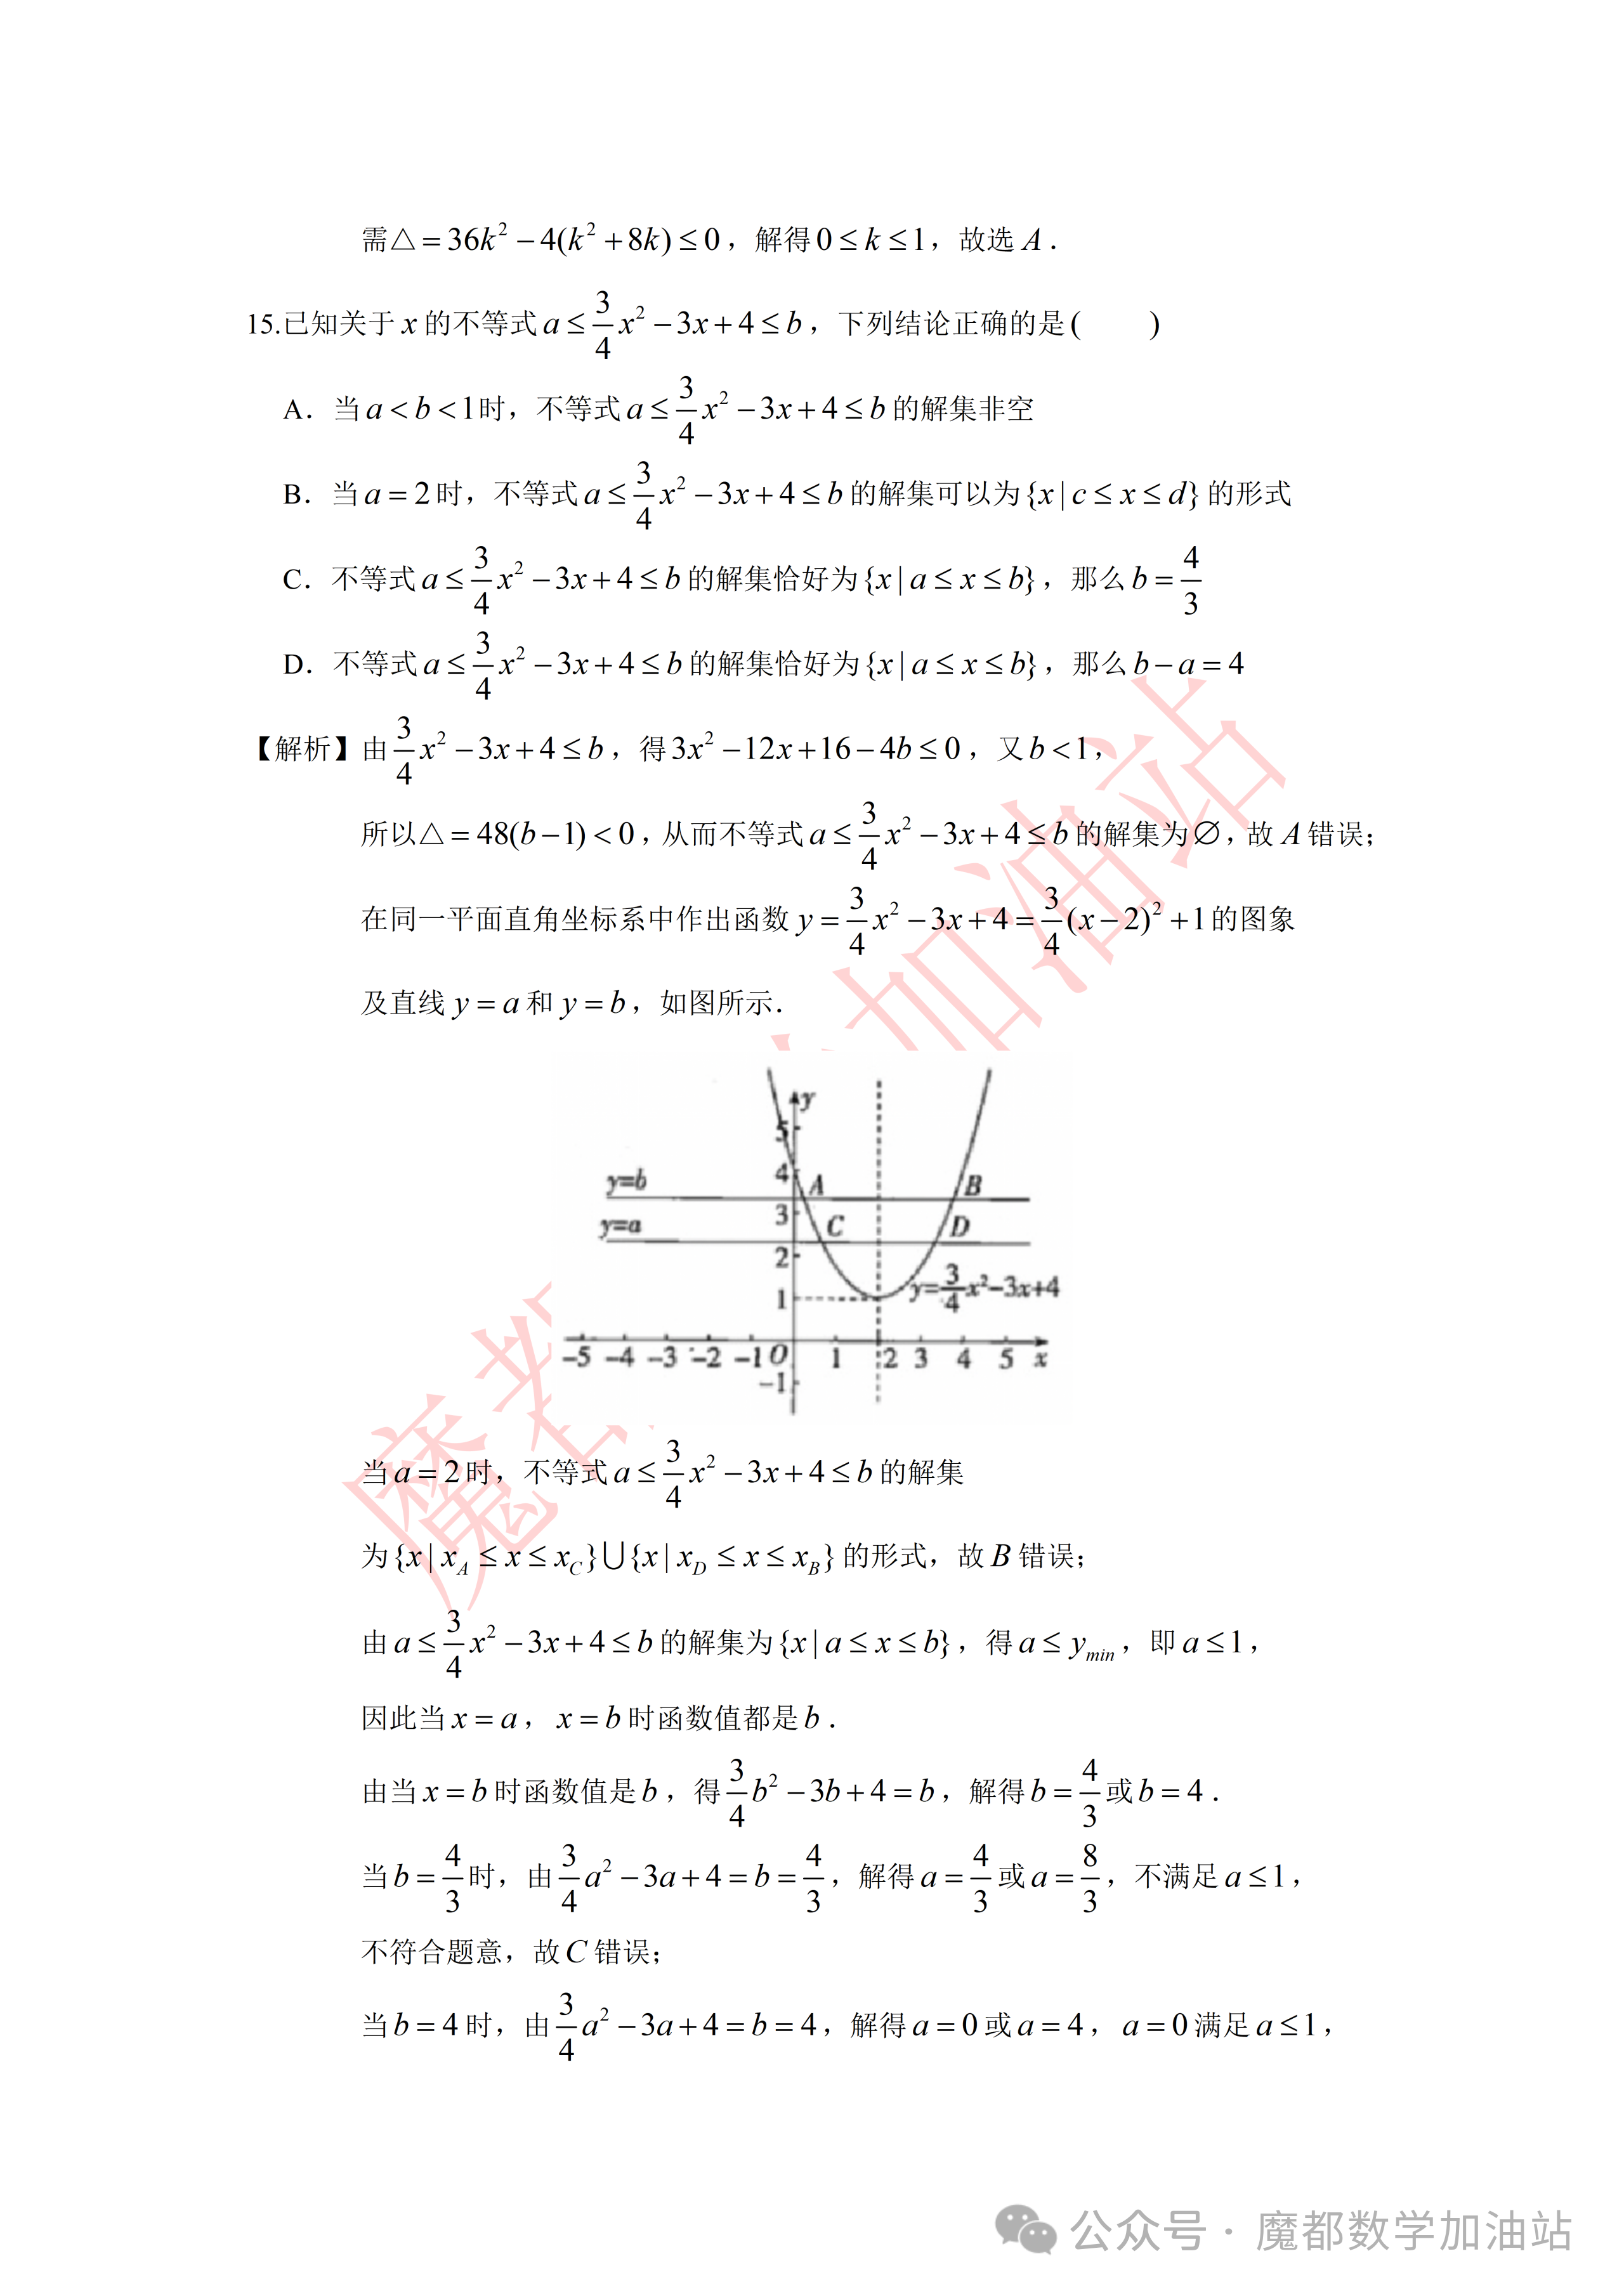
\includegraphics[width=.55\linewidth,trim=900bp 1400bp 760bp 1680bp,clip]{../原图/高一46_交附闵行_国庆作业3/05.png}
\end{center}
\step{当 $a=2$ 时，不等式 $a\leqslant\dfrac34x^2-3x+4\leqslant b$ 的解集为
$\{x\mid x_A\leqslant x\leqslant x_C\}\cup\{x\mid x_D\leqslant x\leqslant x_B\}$ 的形式，故 $B$ 错误；}
\step{由 $a\leqslant\dfrac34x^2-3x+4\leqslant b$ 的解集恰好为 $\{x\mid a\leqslant x\leqslant b\}$ 的形式，得 $a\leqslant y_{\min}$，即 $a\leqslant1$，}
\step{因为当 $x=a$、$x=b$ 时函数值都是 $b$，当 $x=a$ 时，$\dfrac34a^2-3a+4=b$；当 $x=b$ 时，$\dfrac34b^2-3b+4=b$，}
\step{解得 $b=\dfrac43$ 或 $b=4$，}
\step{当 $b=\dfrac43$ 时，由 $\dfrac34a^2-3a+4=b$，解得 $a=\dfrac43$ 或 $a=\dfrac83$，不符合题意，故 $C$ 错误；}
\step{当 $b=4$ 时，由 $\dfrac34a^2-3a+4=b$，解得 $a=0$ 或 $a=4$，$a=0$ 满足 $a\leqslant1$，故 $D$ 正确；}
\step{故选 $D$.}
\solend
\fi

\item 已知 $x$、$y\in(0,+\infty)$，则 $(x-y)^2+2y+1-x+\dfrac4x$ 的最小值为\mbox{（\quad）}

\keepwithprev
A. $1$\qquad B. $2$\qquad C. $3$\qquad D. $4$

\ans{$D$}

\ifanswer
\solbegin
\step{因为 $(x-y)^2+2y+1-x+\dfrac4x=(x-y-1)^2+x+\dfrac4x$，}
\step{当且仅当 $x-y-1=0$，且 $x=\dfrac4x$ 时取等号，}
\step{又因为 $x+\dfrac4x\geqslant2\sqrt{x\cdot\dfrac4x}=4$，当且仅当 $x=2$ 时取等号，}
\step{故选 $D$.}
\solend
\fi

\end{enumerate}

\bigsec{三、解答题}

\begin{enumerate}
\setcounter{enumi}{16}

\item 设集合 $A=\left\{x\middle|\dfrac{x-3}{x-1}<0\right\}$，$B=\{x\mid x^2-2ax+a^2-1>0\}$.
\begin{enumerate}[label=(\arabic*)]
\item 若 $a=3$，求 $A\cup B$；
\item 若“$x\in A$”是“$x\in B$”的充分条件，求实数 $a$ 的取值范围.
\end{enumerate}

\ifanswer
\solbegin
% 注：原卷题干为 a^2-1，故 a=3 时常数项为 8；题干与本步一致。
\stepm{(1)}{当 $a=3$ 时，$B=\{x\mid x^2-6x+8>0\}=\{x\mid x<2\text{ 或 }x>4\}$；}
\step{因为 $A=\left\{x\middle|\dfrac{x-3}{x-1}<0\right\}=\{x\mid(x-1)(x-3)<0\}=\{x\mid1<x<3\}$，}
\step{所以 $A\cup B=\{x\mid x<2\text{ 或 }x>4\}\cup\{x\mid1<x<3\}
=\{x\mid x<3\text{ 或 }x>4\}$.}
\stepm{(2)}{因为“$x\in A$”是“$x\in B$”的充分条件，所以 $A\subseteq B$，}
\step{因 $A=\left\{x\middle|\dfrac{x-3}{x-1}<0\right\}
=\{x\mid(x-1)(x-3)<0\}=\{x\mid1<x<3\}$，}
\step{所以 $A\subseteq B=\{x\mid x<a-1\text{ 或 }x>a+1\}$，}
\step{要使 $A\subseteq B$，需有 $a-1\geqslant3$ 或 $a+1\leqslant1$，}
\step{所以 $a\geqslant4$ 或 $a\leqslant0$，故 $a$ 的取值范围为 $\{a\mid a\geqslant4\text{ 或 }a\leqslant0\}$.}
\solend
\fi

\ansspace[6]

\item 某学校引入种植类劳动教育课程，打算围成如图所示的四块全等的长方形田地种植不同种类的蔬菜，其中一面可以利用原有的墙（足够长），其他各面需要用篱笆围成，设其中一块田地为矩形 $ABCD$.

\begin{center}
% 原图第 6 页配图直接裁取。
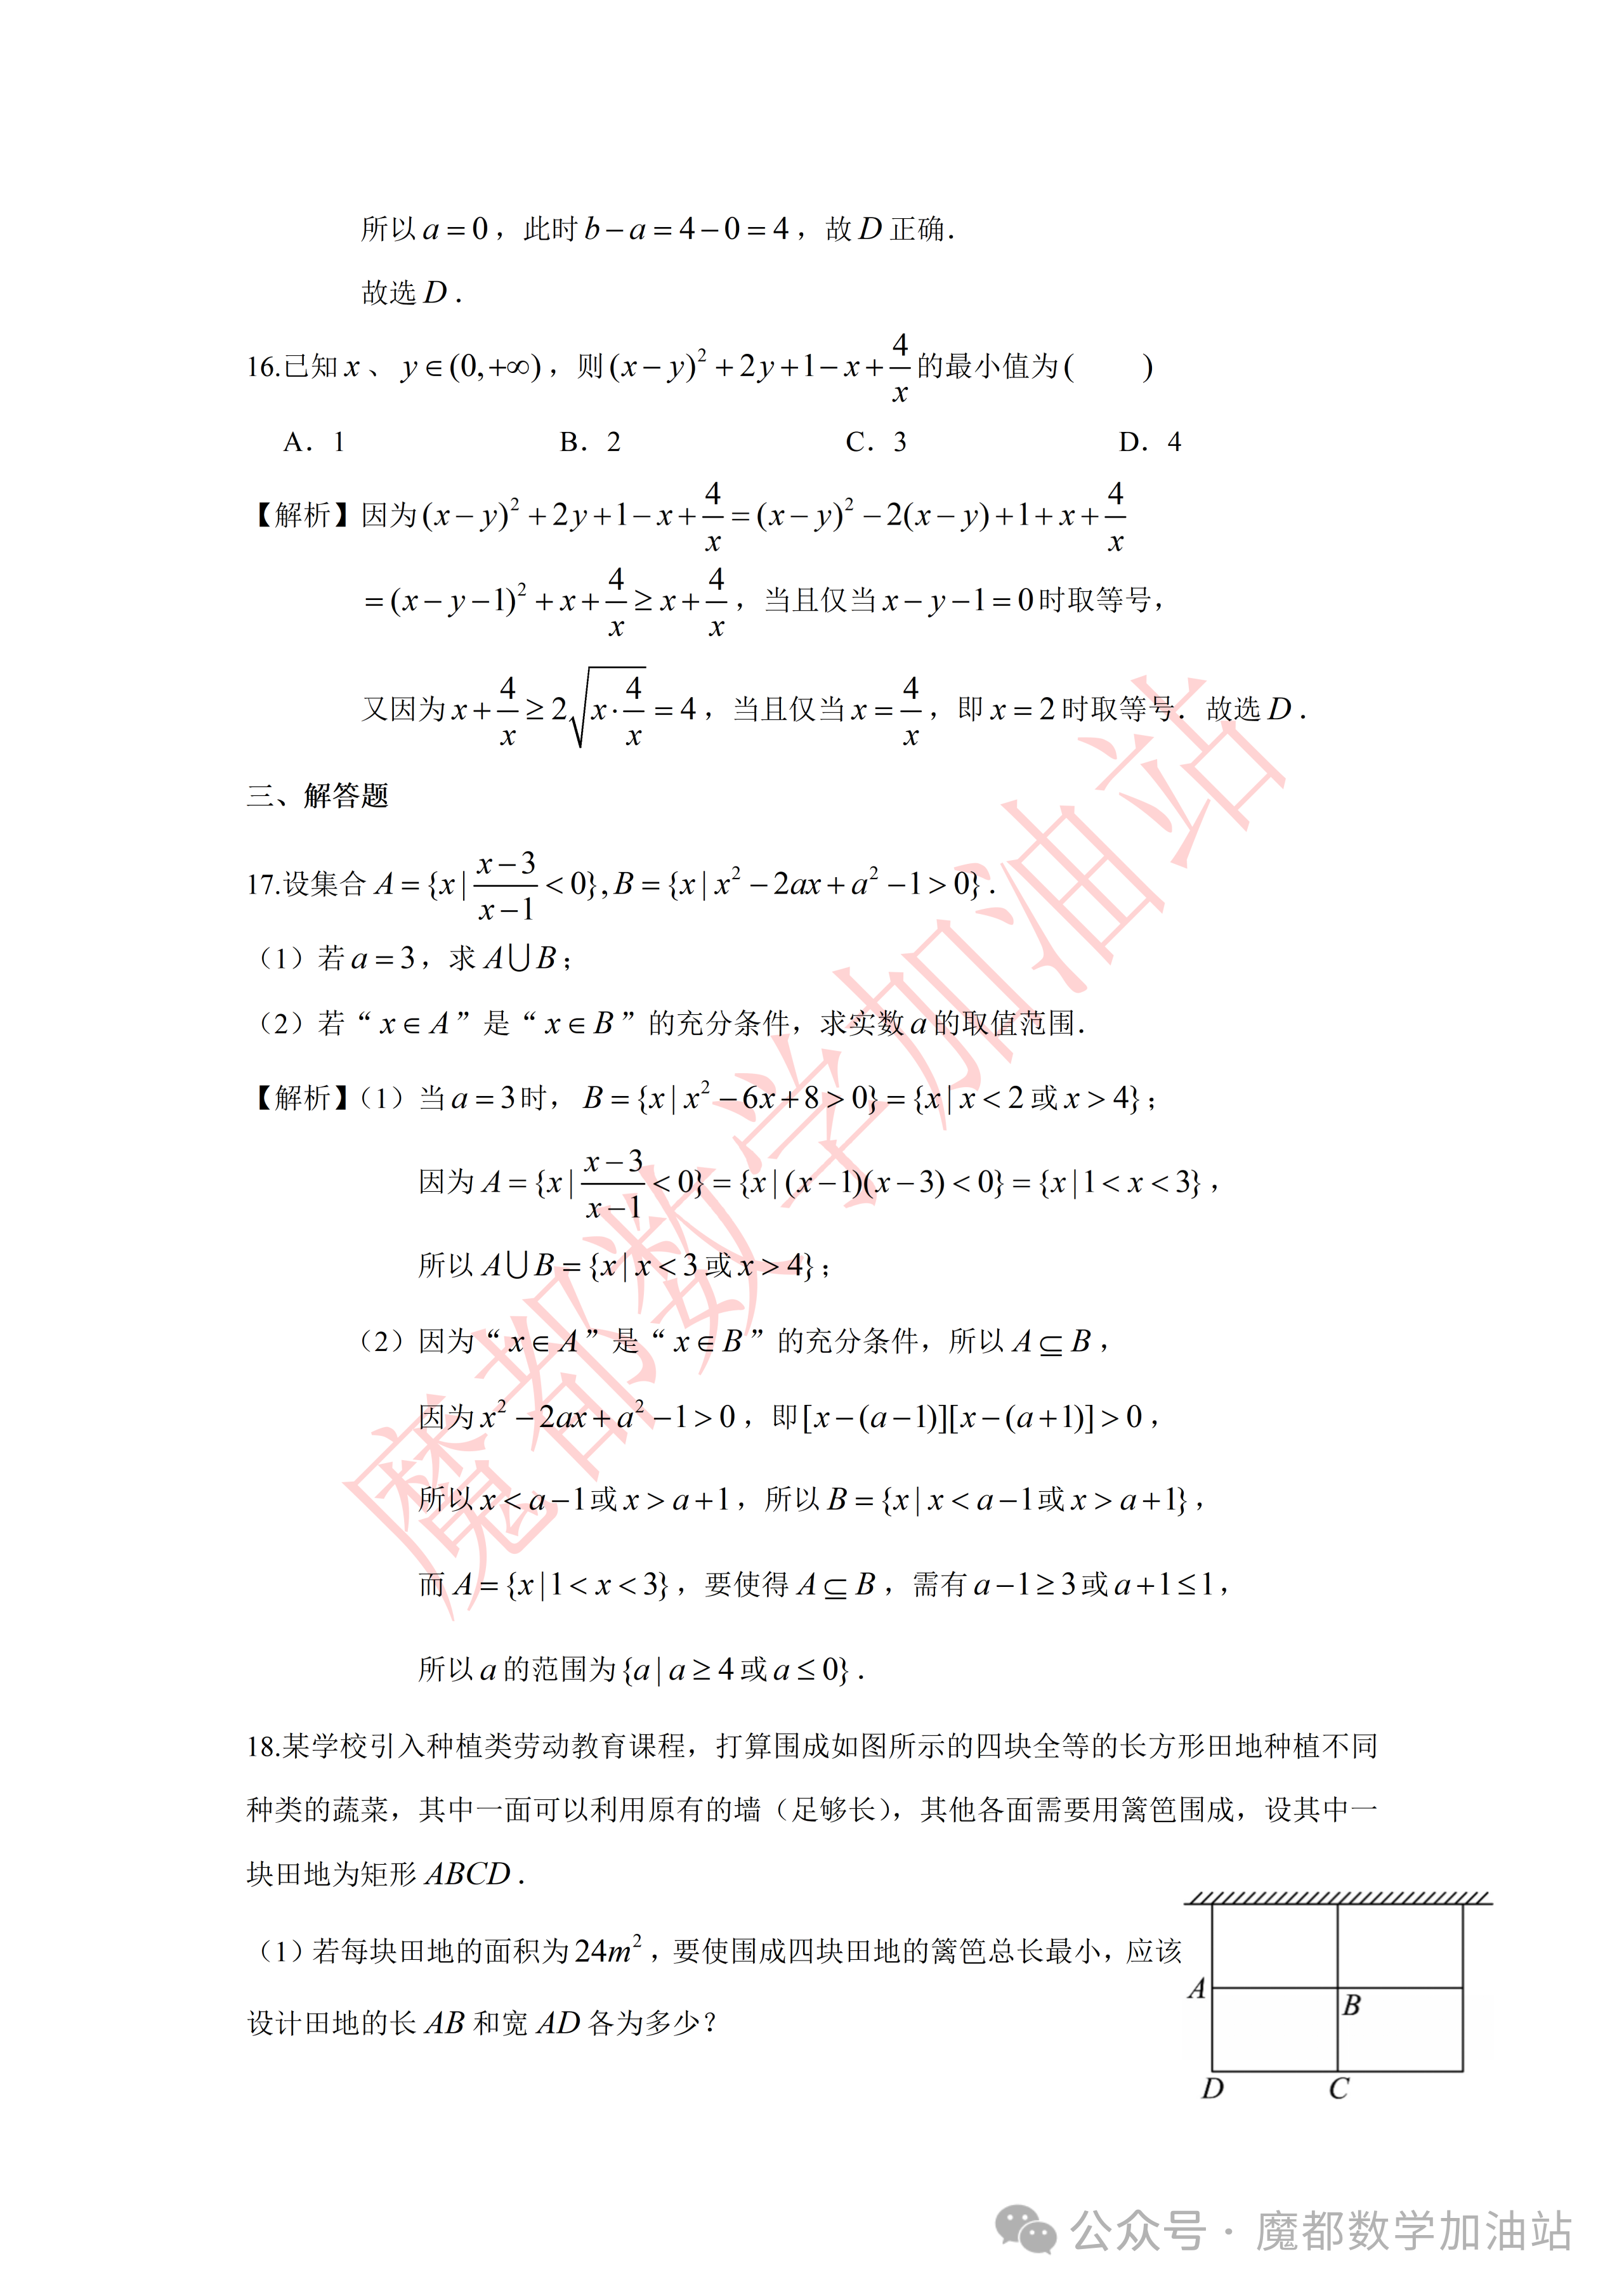
\includegraphics[width=.33\linewidth,trim=1866bp 220bp 210bp 2960bp,clip]{../原图/高一46_交附闵行_国庆作业3/06.png}
\end{center}

\begin{enumerate}[label=(\arabic*)]
\item 若每块田地的面积为 $24\,\text{m}^2$，要使围成四块田地的篱笆总长最小，应该设计田地的长 $AB$ 和宽 $AD$ 各为多少？
\item 现有 $40\,\text{m}$ 长的篱笆，要使每块田地的面积最大，应该设计田地的长 $AB$ 和宽 $AD$ 各为多少？
\end{enumerate}

\ifanswer
\solbegin
\stepm{(1)}{设 $AB$ 长为 $x\,\text{m}$，$AD$ 宽为 $y\,\text{m}$，由题意得 $xy=24$，篱笆总长为 $4x+6y$，}
\step{$4x+6y\geqslant2\sqrt{4x\cdot6y}=2\sqrt{24xy}=48$，}
\step{当且仅当 $4x=6y$ 时取等号，解得 $x=6$，$y=4$，}
\step{所以田地的长 $AB$ 为 $6\,\text{m}$，宽 $AD$ 为 $4\,\text{m}$.}
\stepm{(2)}{设 $AB$ 长为 $a\,\text{m}$，$AD$ 宽为 $b\,\text{m}$，由篱笆总长 $4a+6b=40$，即 $2a+3b=20$，}
\step{将 $a=\dfrac{20-3b}{2}$ 代入每块田地面积 $ab$，得 $ab=\dfrac12b(20-3b)=-\dfrac32b^2+10b$，}
\step{当 $b=\dfrac{10}{3}$ 时，$ab$ 最大，此时 $a=5$，}
\step{所以田地的长 $AB$ 为 $5\,\text{m}$，宽 $AD$ 为 $\dfrac{10}{3}\,\text{m}$.}
\solend
\fi

\ansspace[8]

\item 已知 $x_1$、$x_2$ 是一元二次方程 $4kx^2-4kx+k+1=0$ 的两个不等实数根.
\begin{enumerate}[label=(\arabic*)]
\item 若 $x_1$、$x_2$ 均为正根，求实数 $k$ 的取值范围；
\item 求使 $\dfrac{x_1}{x_2}+\dfrac{x_2}{x_1}-2$ 的值为整数 $k$ 的整数值.
\end{enumerate}

\ifanswer
\solbegin
\stepm{(1)}{由题意，$x_1$、$x_2$ 是方程 $4kx^2-4kx+k+1=0$ 的两个不等实数根，}
\step{故 $k\neq0$，$\Delta=(-4k)^2-16k(k+1)>0$，得 $-16k>0$，所以 $k<0$，}
\step{又 $x_1+x_2=1$，$x_1x_2=\dfrac{k+1}{4k}>0$，得 $k+1<0$，}
\step{所以 $k$ 的取值范围为 $(-\infty,-1)$.}
\stepm{(2)}{由题意，}
\step{$\dfrac{x_1}{x_2}+\dfrac{x_2}{x_1}-2
=\dfrac{x_1^2+x_2^2-2x_1x_2}{x_1x_2}
=\dfrac{(x_1+x_2)^2-4x_1x_2}{x_1x_2}$，}
\step{又 $x_1+x_2=1$，$x_1x_2=\dfrac{k+1}{4k}$，}
\step{则 $\dfrac{x_1}{x_2}+\dfrac{x_2}{x_1}-2=-\dfrac4{k+1}$，}
\step{由于 $-\dfrac4{k+1}$ 为整数，故 $k+1$ 只能取 $\pm1$、$\pm2$、$\pm4$，又 $k<-1$，}
\step{所以整数 $k$ 的值为 $-2$、$-3$、$-5$.}
\solend
\fi

\ansspace[8]

\item 已知 $a>0$，$b>0$，且 $2a+3b=3$.
\begin{enumerate}[label=(\arabic*)]
\item 求 $ab$ 的最大值；
\item 求 $a-\dfrac1{6b}$ 的最大值；
\item 求 $\dfrac2a+\dfrac3{b+1}$ 的最小值.
\end{enumerate}

\ifanswer
\solbegin
\stepm{(1)}{由 $2a+3b=3$，得 $3=2a+3b\geqslant2\sqrt{6ab}$，}
\step{所以 $ab\leqslant\dfrac38$，当且仅当 $2a=3b=\dfrac32$ 时取等号，}
\step{故 $ab$ 的最大值为 $\dfrac38$.}
\stepm{(2)}{由 $2a+3b=3$，得 $a=\dfrac32-\dfrac32b$，}
\step{则 $a-\dfrac1{6b}=\dfrac32-\dfrac32b-\dfrac1{6b}$，}
\step{由基本不等式，$\dfrac32b+\dfrac1{6b}\geqslant2\sqrt{\dfrac32b\cdot\dfrac1{6b}}=1$，}
\step{当且仅当 $\dfrac32b=\dfrac1{6b}$，即 $b=\dfrac13$、$a=1$ 时取等号，}
\step{所以 $a-\dfrac1{6b}$ 的最大值为 $\dfrac12$.}
\stepm{(3)}{由 $2a+3b=3$，得 $2a+3(b+1)=6$，}
\step{$\dfrac2a+\dfrac3{b+1}
=\dfrac16\left(2a+3(b+1)\right)\left(\dfrac2a+\dfrac3{b+1}\right)$}
\step{$=\dfrac16\left(13+\dfrac{6(b+1)}a+\dfrac{6a}{b+1}\right)
\geqslant\dfrac16\left(13+2\sqrt{\dfrac{6(b+1)}a\cdot\dfrac{6a}{b+1}}\right)=\dfrac{25}{6}$，}
\step{当且仅当 $a=b+1$，即 $a=\dfrac65$、$b=\dfrac15$ 时取等号，}
\step{所以 $\dfrac2a+\dfrac3{b+1}$ 的最小值为 $\dfrac{25}{6}$.}
\solend
\fi

\ansspace[8]

\item 已知 $U=\R$ 为全集，集合 $A=\{s^2+3t^2\mid s,t\in U\}$.
\begin{enumerate}[label=(\arabic*)]
\item 设 $U=\{1,3,5\}$，求集合 $A$ 的元素个数；
\item 设 $U=\Z$，证明：若 $x\in A$，则 $7x\in A$；
\item 设 $U=\R$，$x$、$y\in A$，且 $x=m^2+3n^2$，$y=p^2+3q^2$，若 $mp-3nq=\sqrt3$，求 $x+y+mq+np$ 的最小值.
\end{enumerate}

\ifanswer
\solbegin
\stepm{(1)}{当 $s=1$，$t=1$ 时，$s^2+3t^2=1+3=4$；}
\step{当 $s=1$，$t=3$ 时，$s^2+3t^2=1+27=28$；}
\step{当 $s=1$，$t=5$ 时，$s^2+3t^2=1+75=76$；}
\step{当 $s=3$，$t=1$ 时，$s^2+3t^2=9+3=12$；}
\step{当 $s=3$，$t=3$ 时，$s^2+3t^2=9+27=36$；}
\step{当 $s=3$，$t=5$ 时，$s^2+3t^2=9+75=84$；}
\step{当 $s=5$，$t=1$ 时，$s^2+3t^2=25+3=28$；}
\step{当 $s=5$，$t=3$ 时，$s^2+3t^2=25+27=52$；}
\step{当 $s=5$，$t=5$ 时，$s^2+3t^2=25+75=100$，}
\step{所以 $A=\{4,12,28,36,52,76,84,100\}$，有 $8$ 个元素.}
\stepm{(2)}{因为 $U=\Z$，$x\in A$，设 $x=s^2+3t^2$，}
\step{则 $7x=7(s^2+3t^2)=(2s+3t)^2+3(s-2t)^2\in A$，}
\step{所以 $7x\in A$.}
\stepm{(3)}{因为 $x=m^2+3n^2$，$y=p^2+3q^2$，}
\step{$xy=(m^2+3n^2)(p^2+3q^2)=3(mq+np)^2+(mp-3nq)^2$，}
\step{设 $mq+np=b$，则 $xy=3b^2+3$，所以 $y=\dfrac{3b^2+3}{x}$，}
\step{于是 $x+y+mq+np=x+\dfrac{3b^2+3}{x}+b\geqslant2\sqrt{3b^2+3}+b$，}
\step{设 $2\sqrt{3b^2+3}+b=t$，整理得 $11b^2+2bt+12-t^2=0$，}
\step{判别式法，$\Delta=4t^2-44(12-t^2)\geqslant0$，得 $t\geqslant\sqrt{11}$，}
\step{即 $(x+y+mq+np)_{\min}=\sqrt{11}$，所以 $x+y+mq+np$ 的最小值为 $\sqrt{11}$.}
\solend
\fi

\ansspace*[10]

\end{enumerate}

\end{document}
"
% 紧凑版：xelatex "\def\iscompact{1}% 高一46_交附闵行_国庆作业3.tex
%   —— 高一上数学“2026-2027 年交附闵行高一上国庆作业 3”（讲评版）
% 试卷版：xelatex 高一46_交附闵行_国庆作业3.tex
% 答案版：xelatex "\def\isanswer{1}\input{高一46_交附闵行_国庆作业3.tex}"
% 紧凑版：xelatex "\def\iscompact{1}\input{高一46_交附闵行_国庆作业3.tex}"
%
% 原始材料：微信公众号“魔都数学加油站”，作者破晓，2026-10-02 17:56 发布。
% 原文标题：“27学年高一46——2026-2027你那上海市交附闵行高一上国庆作业3”
% （公众号标题中的“你那”照录，系原文标题字样）；原文链接：
% http://mp.weixin.qq.com/s?__biz=Mzg4ODU1ODMxOQ==&mid=2247591657&idx=3&sn=a894d1a16611283a61b3eaba32a3f24c&chksm=cee83366c6a55381b370069f84ef63d20251f94608bb37cc4ec2d66227401bd147f4f6bd8256&scene=126&sessionid=1790935402&subscene=7&clicktime=1790937618&enterid=1790937618#rd
% 正文为 9 张 PNG 页，按页序读取原图；第 01、02、07 页 4762×6735，
% 第 03—06、08、09 页 2560×3620。卷面标题照原卷印作“2026-2027 年交附闵行高一上国庆作业 3”。
% 原文从第 3 题起，题号照原卷保留；正文为讲评版，答案、解析依原卷顺序录入。
% 水印及页脚公众号标识不录入。卷面插图直接裁取对应原图页，不另制图片文件。
%
% 与原卷的排版差异：
%   ① 原卷按“一、填空题”“二、选择题”“三、解答题”分节，本稿沿用原节与原题号，
%      只改排为全稿统一的大节样式；
%   ② 原卷答案与解析依页面位置分布，本稿按 common.sty 统一置于答案版；
%   ③ 原卷副标题未印，本稿按“知识模块”口径标作“集合与常用逻辑用语、不等式”。
%
% 原卷存疑一处（照抄未改，见第 12 题题干及解析处注释）：
%   第 12 题题干同时给出 x∈Z，却称不等式组有“50 个不等的实数解”；解析按整数根计数。
%   此处题干与解析的原文不一致，本稿均照录。
% 第 17 题曾疑似有常数项不一致：复核原图题干为 a^2-1，a=3 时常数项确为 8，
% 与解析相符；不将其记作原卷错误。
%
\documentclass[a4paper,11pt]{article}
\usepackage{common}

\begin{document}

\examtitlest[3]{2026--2027 年交附闵行高一上国庆作业 3}{集合与常用逻辑用语、不等式}

\bigsec{一、填空题}

\begin{enumerate}
\setcounter{enumi}{2}

\item 不等式 $\dfrac{x^2-10}{x+2}\geqslant1$ 的解集为\blankline[4.4em].

\ifanswer
\ans{$\{x\mid-3\leqslant x<-2\text{ 或 }x\geqslant4\}$}
\solbegin
\step{不等式 $\dfrac{x^2-10}{x+2}\geqslant1$，移项得 $\dfrac{x^2-10}{x+2}-1\geqslant0$，}
\step{通分得 $\dfrac{x^2-x-12}{x+2}\geqslant0$，即 $\dfrac{(x-4)(x+3)}{x+2}\geqslant0$，}
\step{解得 $-3\leqslant x<-2$ 或 $x\geqslant4$，}
\step{故不等式的解集为 $\{x\mid-3\leqslant x<-2\text{ 或 }x\geqslant4\}$.}
\solend
\fi

\item $|x-3|+|x-5|\geqslant2$，当等号成立时，$x$ 的范围是\blankline[4.4em].

\ifanswer
\ans{$[3,5]$}
\fi

\item 若直角三角形斜边长等于 $4\sqrt2\,\text{cm}$，则直角三角形面积的最大值为\blankline[4.4em].

\ifanswer
\solbegin
\step{设 $Rt\triangle ABC$ 中，$C=90^\circ$，则 $c=\sqrt{a^2+b^2}=4\sqrt2$，所以 $a^2+b^2=32$，}
\step{由基本不等式得 $a^2+b^2\geqslant2ab$，当且仅当 $a=b=4$ 时取等号，}
\step{所以 $\triangle ABC$ 的面积 $S=\dfrac12ab\leqslant8$，}
\step{当且仅当 $a=b=4$ 时，$\triangle ABC$ 的面积最大值为 $8$.}
\solend
\fi

\item 不等式 $(x-1)(2-x)>0$ 的解集为\blankline[4.4em].

\ifanswer
\solbegin
\step{$(x-1)(2-x)>0\Rightarrow(x-1)(x-2)<0$，}
\step{故不等式的解集为 $\{x\mid1<x<2\}$.}
\solend
\fi

\item 已知集合 $A=\{1,2\}$，$B=\{x\mid x^2-2mx+m=0\}$，$A\cup B=A$，则实数 $m$ 的取值范围为\blankline[4.4em].

\ifanswer
\solbegin
\step{因为 $A\cup B=A$，所以 $B\subseteq A$，}
\step{当 $B=\varnothing$ 时，$\Delta=(-2m)^2-4m<0$，解得 $0<m<1$，}
\step{当 $B$ 为单元素集时，$\Delta=0$，解得 $m=0$ 或 $m=1$，}
\step{当 $m=0$ 时，方程 $x^2=0$，解得 $x=0$，此时 $B=\{0\}$，不满足 $B\subseteq A$；}
\step{当 $m=1$ 时，方程 $x^2-2x+1=0$，解得 $x=1$，此时 $B=\{1\}$，满足 $B\subseteq A$；}
\step{当 $B=\{1,2\}$ 时，由韦达定理得 $1+2=2m$，$1\times2=m$，无解，}
\step{综上所述，实数 $m$ 的取值范围为 $\{m\mid0<m\leqslant1\}$.}
\solend
\fi

\item 设 $a$、$b$、$c\in\R^+$，若 $a+b+c=1$，则 $\dfrac1a+\dfrac1b+\dfrac1c\geqslant$\blankline[4.4em].

\ifanswer
\solbegin
\step{因为 $a$、$b$、$c\in\R^+$，且 $a+b+c=1$，}
\step{所以 $\dfrac1a+\dfrac1b+\dfrac1c=(a+b+c)\left(\dfrac1a+\dfrac1b+\dfrac1c\right)$}
\step{$=3+\dfrac ab+\dfrac ba+\dfrac ac+\dfrac ca+\dfrac bc+\dfrac cb$，}
\step{由基本不等式得 $\dfrac ab+\dfrac ba\geqslant2$，$\dfrac ac+\dfrac ca\geqslant2$，$\dfrac bc+\dfrac cb\geqslant2$，}
\step{所以 $\dfrac1a+\dfrac1b+\dfrac1c\geqslant9$，当且仅当 $a=b=c=\dfrac13$ 时取等号，}
\step{所以 $\dfrac1a+\dfrac1b+\dfrac1c$ 的最小值为 $9$.}
\solend
\fi

\item 已知 $-1\leqslant x+y\leqslant2$，$-2\leqslant x-y\leqslant1$，则 $x-2y$ 的范围为\blankline[4.4em].

\ifanswer
\solbegin
\step{设 $x-2y=m(x+y)+n(x-y)$，}
\step{则 $x-2y=(m+n)x+(m-n)y$，所以 $m+n=1$，$m-n=-2$，}
\step{解得 $m=-\dfrac12$，$n=\dfrac32$，}
\step{所以 $x-2y=-\dfrac12(x+y)+\dfrac32(x-y)$，}
\step{因为 $-1\leqslant x+y\leqslant2$，$-2\leqslant x-y\leqslant1$，}
\step{所以 $-4\leqslant x-2y\leqslant2$，即 $x-2y$ 的范围为 $[-4,2]$.}
\solend
\fi

\item 设集合 $A=\{1,2,m\}$，其中 $m$ 为实数，令 $B=\{a^2\mid a\in A\}$，$C=A\cup B$. 若 $C$ 中所有元素之和为 $6$，则 $C$ 中的所有元素之积为\blankline[4.4em].

\ifanswer
\solbegin
\step{因为 $A=\{1,2,m\}$，所以 $B=\{a^2\mid a\in A\}=\{1,4,m^2\}$，$m\neq1$，$m\neq2$，}
\step{又 $C=A\cup B$，所以 $1\in C$，$4\in C$，$m^2\in C$，}
\step{若 $m^2=1$，则 $m=-1$ 或 $m=1$（舍），当 $m=-1$ 时，$C=\{1,2,4,-1\}$，$C$ 中所有元素之和为 $6$，}
\step{此时 $C$ 中所有元素之积为 $-8$；}
\step{若 $m^2=2$，则 $m=-\sqrt2$ 或 $m=\sqrt2$，$C$ 中所有元素之和不符合题意；}
\step{若 $m^2=4$，则 $m=-2$ 或 $m=2$，此时 $C=\{1,2,4,-2\}$ 或 $C=\{1,2,4\}$，所有元素之和不符合题意；}
\step{若 $m^2\neq1$，$m^2\neq2$，$m^2\neq4$，则 $C=\{1,2,4,m,m^2\}$，}
\step{所以 $1+2+4+m+m^2=6$，即 $m^2+m+1=0$，无解，}
\step{综上所述，$C$ 中所有元素之积为 $-8$.}
\solend
\fi

\item 若对任意实数 $x>0$，$y>0$，不等式 $x+\sqrt{xy}\leqslant a(x+y)$ 恒成立，则实数 $a$ 的最小值为\blankline[4.4em].

\ifanswer
\solbegin
\step{由不等式 $x+\sqrt{xy}\leqslant a(x+y)$ 对任意实数 $x>0$，$y>0$ 恒成立，}
\step{得 $a\geqslant\dfrac{x+\sqrt{xy}}{x+y}$，}
\step{设 $\sqrt{\dfrac yx}=t>0$，则 $a\geqslant\dfrac{1+t}{1+t^2}$，}
\step{$\dfrac{1+t}{1+t^2}\leqslant\dfrac{\sqrt2+1}{2}$，当且仅当 $t=\sqrt2-1$ 时取等号，}
\step{所以实数 $a$ 的最小值为 $\dfrac{\sqrt2+1}{2}$.}
\solend
\fi

% 注：原卷题干给出 x∈Z，却写“实数解”；解析按整数解计数，题干与解析不一致，照录未改。
\item 若关于 $x$ 的不等式组
$\begin{cases}x^2-3mx\geqslant4m^2\\-20<x<120\end{cases}$（$x\in\Z,m>0$）恰有 $50$ 个不等的实数解，则 $m$ 的取值范围为\blankline[4.4em]（结果用区间表示）.

\ifanswer
\solbegin
\step{由 $x^2-3mx\geqslant4m^2$ 以及 $m>0$，解得 $x\leqslant-m$ 或 $x\geqslant4m$，}
\step{由原不等式组恰有 $50$ 个不等的实数解，可画出如下解集区间：}
\begin{center}
% 原图第 4 页数轴图直接裁取。
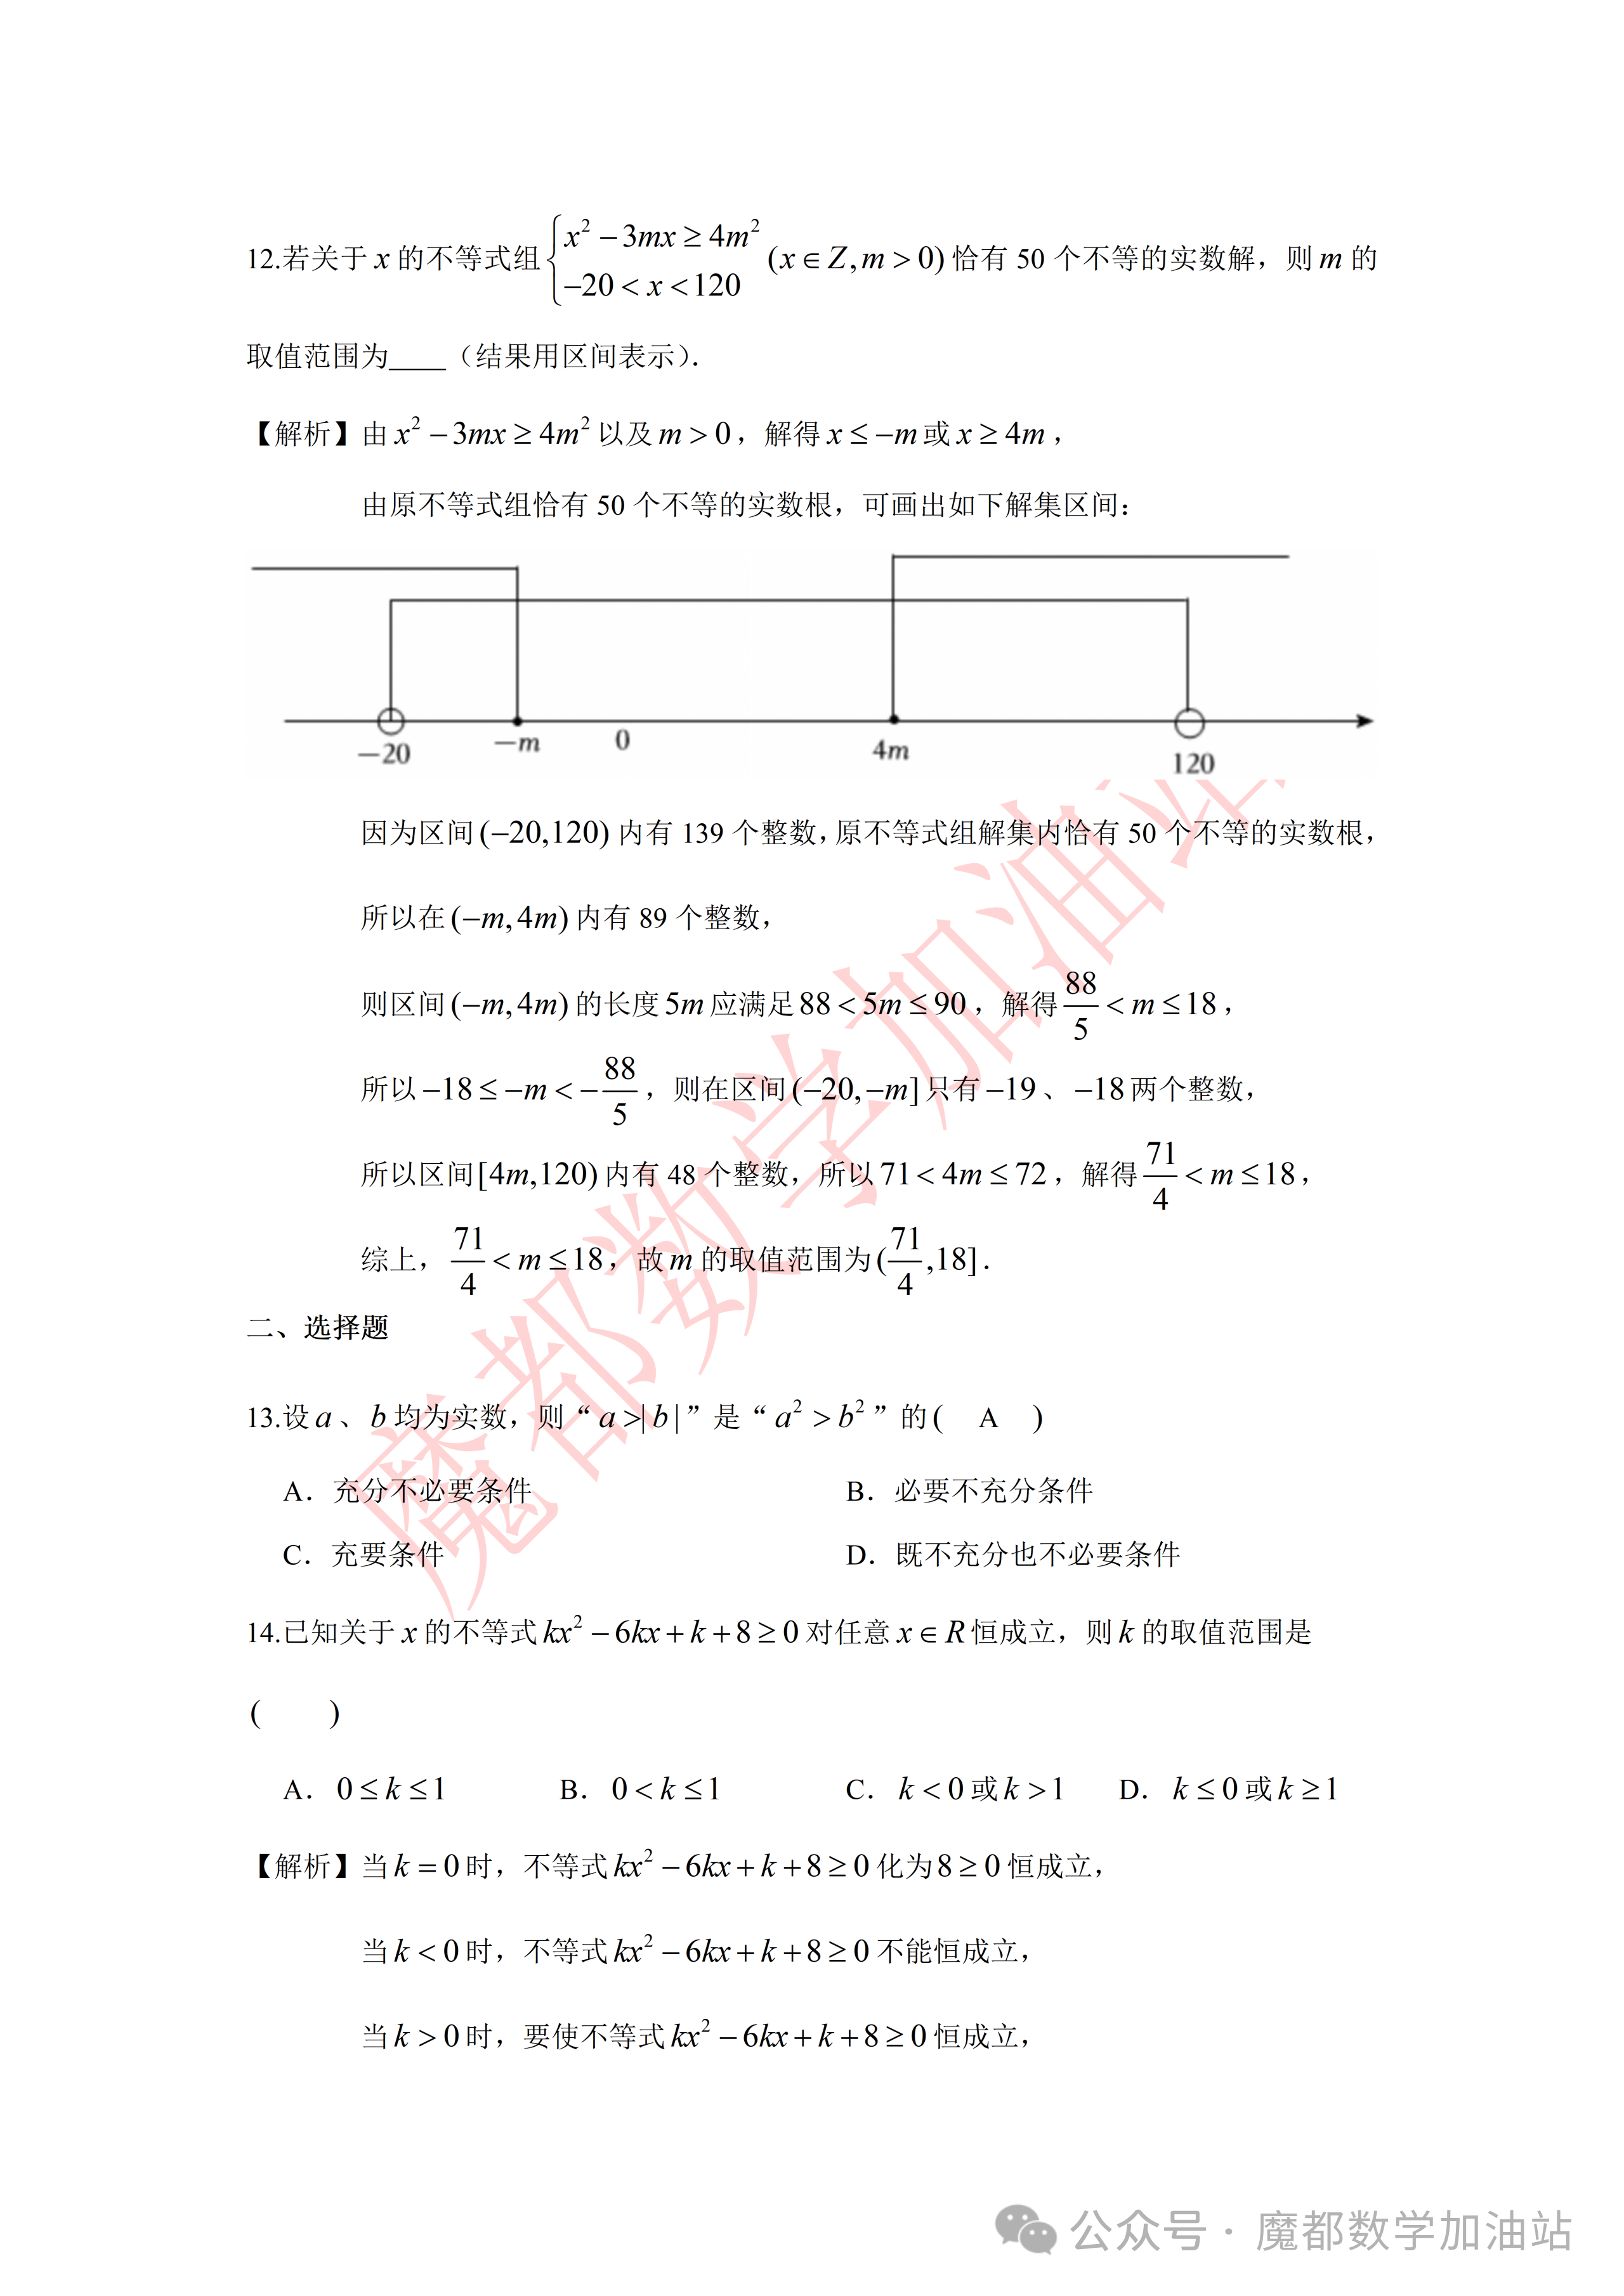
\includegraphics[width=.88\linewidth,trim=400bp 2410bp 320bp 860bp,clip]{../原图/高一46_交附闵行_国庆作业3/04.png}
\end{center}
\step{因为区间 $(-20,120)$ 内有 $139$ 个整数，原不等式组解集内有 $50$ 个不等的整数根，}
\step{所以在区间 $(-m,4m)$ 内有 $89$ 个整数，}
\step{则区间 $(-m,4m)$ 的长度 $5m$ 应满足 $88<5m\leqslant90$，解得 $\dfrac{88}{5}<m\leqslant18$，}
% 注：原卷题干称“实数解”，本行及后文按原卷解析照录为整数根计数。
\step{所以 $-18\leqslant-m<-\dfrac{88}{5}$，则在区间 $(-20,-m]$ 内有 $-19$、$-18$ 两个整数，}
\step{所以区间 $[4m,120)$ 内有 $48$ 个整数，}
\step{则 $71<4m\leqslant72$，解得 $\dfrac{71}{4}<m\leqslant18$，}
\step{综上，$\dfrac{71}{4}<m\leqslant18$，故 $m$ 的取值范围为 $\left(\dfrac{71}{4},18\right]$.}
\solend
\fi

\end{enumerate}

\bigsec{二、选择题}

\begin{enumerate}
\setcounter{enumi}{12}

\item 设 $a$、$b$ 均为实数，则“$a>|b|$”是“$a^2>b^2$”的\mbox{（\quad）}

\keepwithprev
A. 充分不必要条件\qquad B. 必要不充分条件

C. 充要条件\qquad\qquad D. 既不充分也不必要条件

\ans{$A$}

\item 已知关于 $x$ 的不等式 $kx^2-6kx+k+8\geqslant0$ 对任意 $x\in\R$ 恒成立，则 $k$ 的取值范围是\mbox{（\quad）}

\keepwithprev
A. $0\leqslant k\leqslant1$\qquad B. $0<k\leqslant1$

C. $k<0$ 或 $k>1$\qquad D. $k\leqslant0$ 或 $k\geqslant1$

\ans{$A$}

\ifanswer
\solbegin
\step{当 $k=0$ 时，不等式 $kx^2-6kx+k+8\geqslant0$ 化为 $8\geqslant0$ 恒成立，}
\step{当 $k<0$ 时，不等式 $kx^2-6kx+k+8\geqslant0$ 不能恒成立，}
\step{当 $k>0$ 时，要使不等式 $kx^2-6kx+k+8\geqslant0$ 恒成立，}
\step{需 $\Delta=36k^2-4(k^2+8k)\leqslant0$，解得 $0\leqslant k\leqslant1$，故选 $A$.}
\solend
\fi

\item 已知关于 $x$ 的不等式 $a\leqslant\dfrac34x^2-3x+4\leqslant b$，下列结论正确的是\mbox{（\quad）}

\keepwithprev
A. 当 $a<b<1$ 时，不等式 $a\leqslant\dfrac34x^2-3x+4\leqslant b$ 的解集非空

B. 当 $a=2$ 时，不等式 $a\leqslant\dfrac34x^2-3x+4\leqslant b$ 的解集可以为 $\{x\mid c\leqslant x\leqslant d\}$ 的形式

C. 不等式 $a\leqslant\dfrac34x^2-3x+4\leqslant b$ 的解集恰好为 $\{x\mid a\leqslant x\leqslant b\}$，那么 $b=\dfrac43$

D. 不等式 $a\leqslant\dfrac34x^2-3x+4\leqslant b$ 的解集恰好为 $\{x\mid a\leqslant x\leqslant b\}$，那么 $b-a=4$

\ans{$D$}

\ifanswer
\solbegin
\step{由 $\dfrac34x^2-3x+4\leqslant b$，得 $3x^2-12x+16-4b\leqslant0$，又 $b<1$，}
\step{所以 $\Delta=144-12(16-4b)=48(b-1)<0$，从而不等式无解，故 $A$ 错误；}
\step{在同一平面直角坐标系中作出函数 $y=\dfrac34x^2-3x+4=\dfrac34(x-2)^2+1$ 的图象及直线 $y=a$ 和 $y=b$，如图所示.}
\begin{center}
% 原图第 5 页解析配图直接裁取。
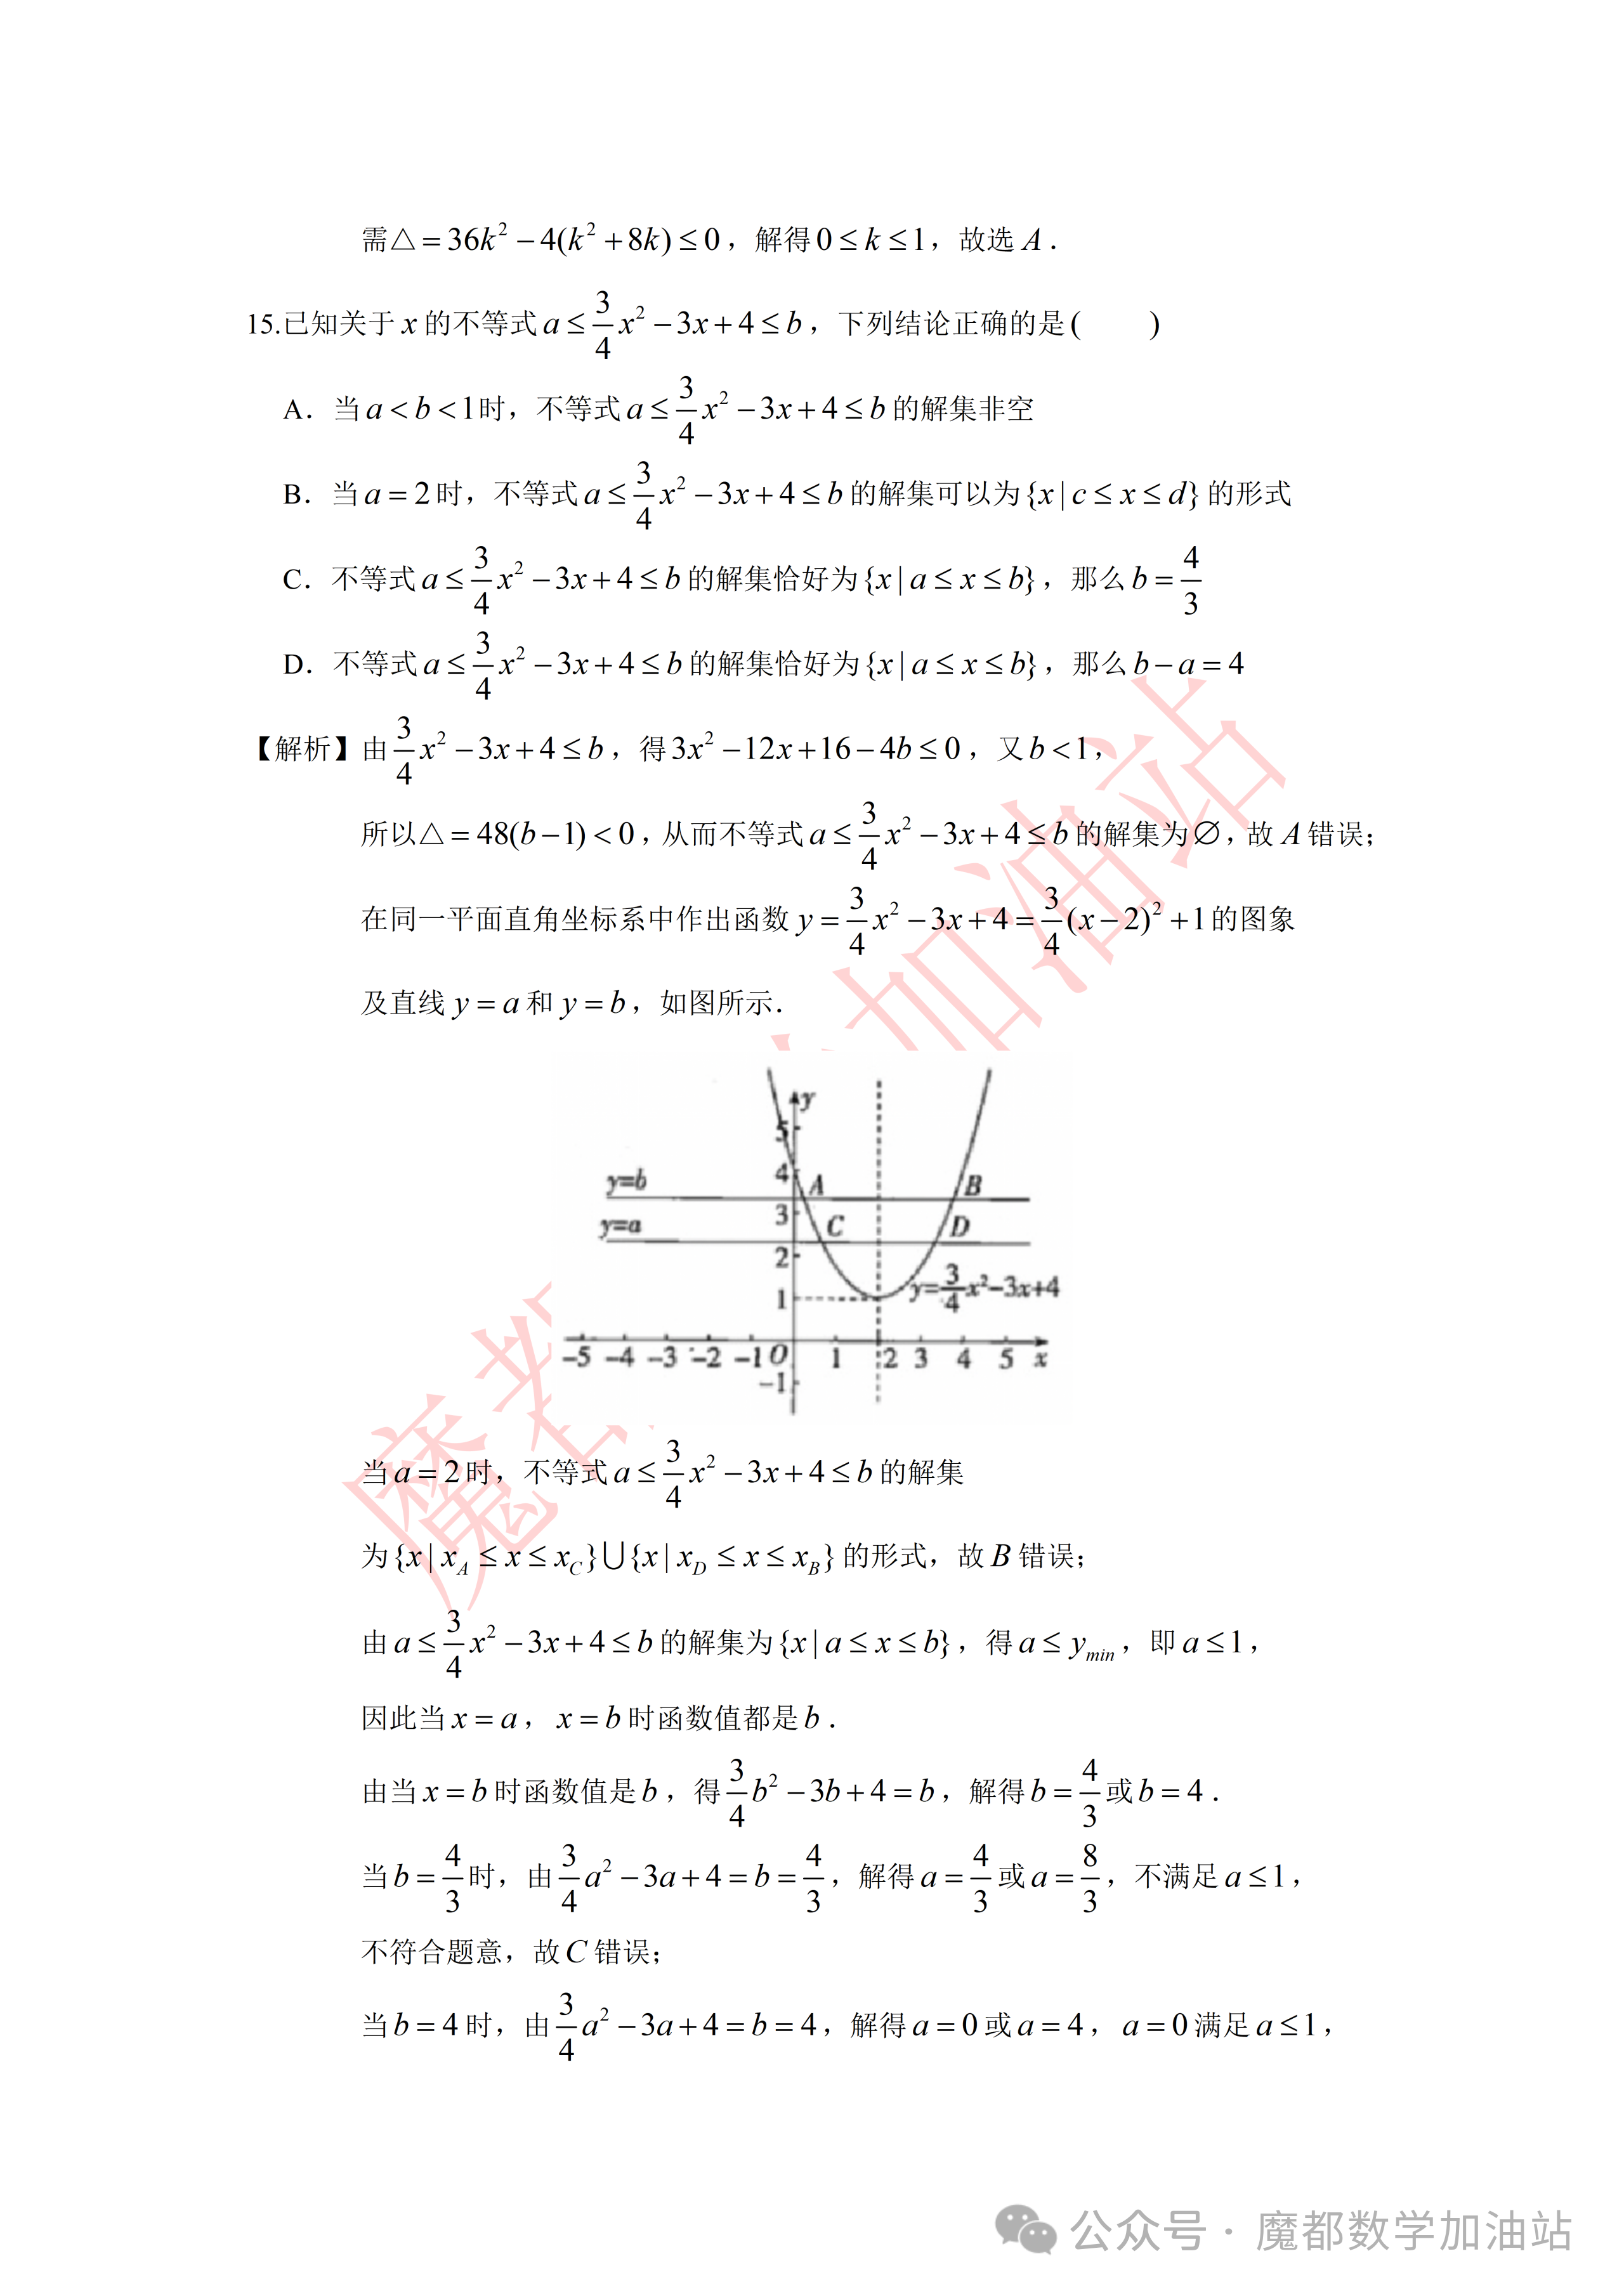
\includegraphics[width=.55\linewidth,trim=900bp 1400bp 760bp 1680bp,clip]{../原图/高一46_交附闵行_国庆作业3/05.png}
\end{center}
\step{当 $a=2$ 时，不等式 $a\leqslant\dfrac34x^2-3x+4\leqslant b$ 的解集为
$\{x\mid x_A\leqslant x\leqslant x_C\}\cup\{x\mid x_D\leqslant x\leqslant x_B\}$ 的形式，故 $B$ 错误；}
\step{由 $a\leqslant\dfrac34x^2-3x+4\leqslant b$ 的解集恰好为 $\{x\mid a\leqslant x\leqslant b\}$ 的形式，得 $a\leqslant y_{\min}$，即 $a\leqslant1$，}
\step{因为当 $x=a$、$x=b$ 时函数值都是 $b$，当 $x=a$ 时，$\dfrac34a^2-3a+4=b$；当 $x=b$ 时，$\dfrac34b^2-3b+4=b$，}
\step{解得 $b=\dfrac43$ 或 $b=4$，}
\step{当 $b=\dfrac43$ 时，由 $\dfrac34a^2-3a+4=b$，解得 $a=\dfrac43$ 或 $a=\dfrac83$，不符合题意，故 $C$ 错误；}
\step{当 $b=4$ 时，由 $\dfrac34a^2-3a+4=b$，解得 $a=0$ 或 $a=4$，$a=0$ 满足 $a\leqslant1$，故 $D$ 正确；}
\step{故选 $D$.}
\solend
\fi

\item 已知 $x$、$y\in(0,+\infty)$，则 $(x-y)^2+2y+1-x+\dfrac4x$ 的最小值为\mbox{（\quad）}

\keepwithprev
A. $1$\qquad B. $2$\qquad C. $3$\qquad D. $4$

\ans{$D$}

\ifanswer
\solbegin
\step{因为 $(x-y)^2+2y+1-x+\dfrac4x=(x-y-1)^2+x+\dfrac4x$，}
\step{当且仅当 $x-y-1=0$，且 $x=\dfrac4x$ 时取等号，}
\step{又因为 $x+\dfrac4x\geqslant2\sqrt{x\cdot\dfrac4x}=4$，当且仅当 $x=2$ 时取等号，}
\step{故选 $D$.}
\solend
\fi

\end{enumerate}

\bigsec{三、解答题}

\begin{enumerate}
\setcounter{enumi}{16}

\item 设集合 $A=\left\{x\middle|\dfrac{x-3}{x-1}<0\right\}$，$B=\{x\mid x^2-2ax+a^2-1>0\}$.
\begin{enumerate}[label=(\arabic*)]
\item 若 $a=3$，求 $A\cup B$；
\item 若“$x\in A$”是“$x\in B$”的充分条件，求实数 $a$ 的取值范围.
\end{enumerate}

\ifanswer
\solbegin
% 注：原卷题干为 a^2-1，故 a=3 时常数项为 8；题干与本步一致。
\stepm{(1)}{当 $a=3$ 时，$B=\{x\mid x^2-6x+8>0\}=\{x\mid x<2\text{ 或 }x>4\}$；}
\step{因为 $A=\left\{x\middle|\dfrac{x-3}{x-1}<0\right\}=\{x\mid(x-1)(x-3)<0\}=\{x\mid1<x<3\}$，}
\step{所以 $A\cup B=\{x\mid x<2\text{ 或 }x>4\}\cup\{x\mid1<x<3\}
=\{x\mid x<3\text{ 或 }x>4\}$.}
\stepm{(2)}{因为“$x\in A$”是“$x\in B$”的充分条件，所以 $A\subseteq B$，}
\step{因 $A=\left\{x\middle|\dfrac{x-3}{x-1}<0\right\}
=\{x\mid(x-1)(x-3)<0\}=\{x\mid1<x<3\}$，}
\step{所以 $A\subseteq B=\{x\mid x<a-1\text{ 或 }x>a+1\}$，}
\step{要使 $A\subseteq B$，需有 $a-1\geqslant3$ 或 $a+1\leqslant1$，}
\step{所以 $a\geqslant4$ 或 $a\leqslant0$，故 $a$ 的取值范围为 $\{a\mid a\geqslant4\text{ 或 }a\leqslant0\}$.}
\solend
\fi

\ansspace[6]

\item 某学校引入种植类劳动教育课程，打算围成如图所示的四块全等的长方形田地种植不同种类的蔬菜，其中一面可以利用原有的墙（足够长），其他各面需要用篱笆围成，设其中一块田地为矩形 $ABCD$.

\begin{center}
% 原图第 6 页配图直接裁取。
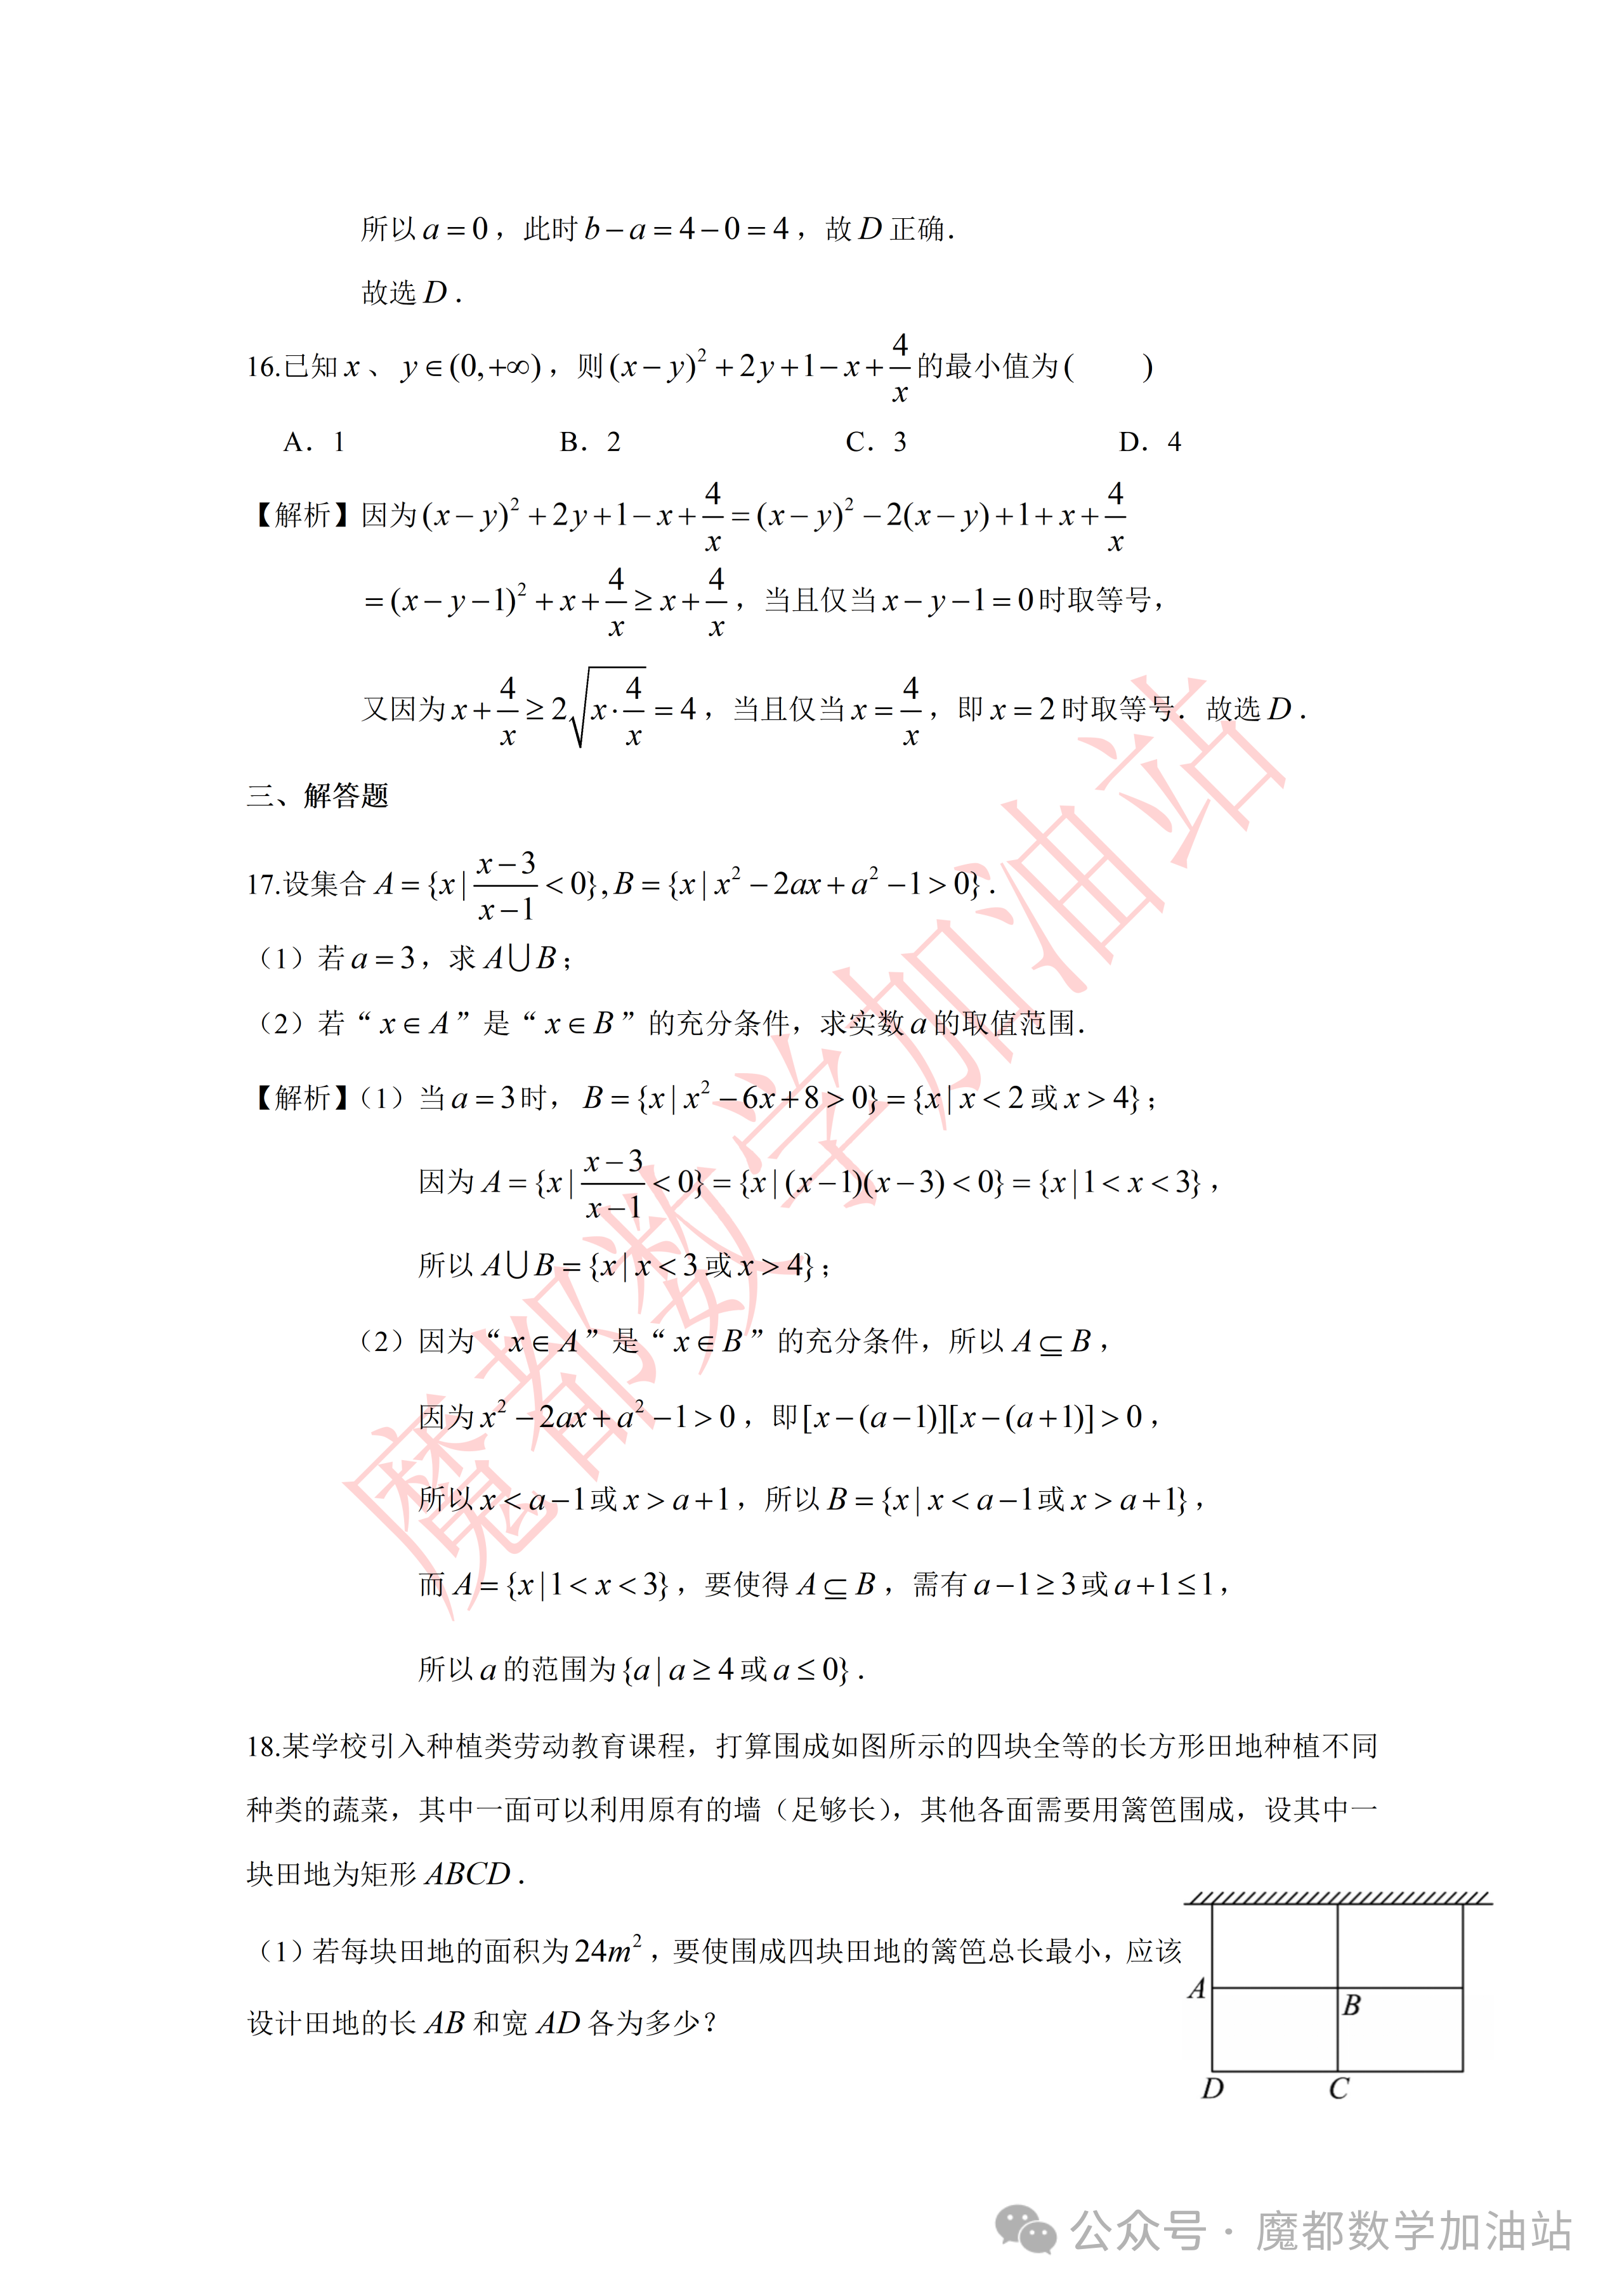
\includegraphics[width=.33\linewidth,trim=1866bp 220bp 210bp 2960bp,clip]{../原图/高一46_交附闵行_国庆作业3/06.png}
\end{center}

\begin{enumerate}[label=(\arabic*)]
\item 若每块田地的面积为 $24\,\text{m}^2$，要使围成四块田地的篱笆总长最小，应该设计田地的长 $AB$ 和宽 $AD$ 各为多少？
\item 现有 $40\,\text{m}$ 长的篱笆，要使每块田地的面积最大，应该设计田地的长 $AB$ 和宽 $AD$ 各为多少？
\end{enumerate}

\ifanswer
\solbegin
\stepm{(1)}{设 $AB$ 长为 $x\,\text{m}$，$AD$ 宽为 $y\,\text{m}$，由题意得 $xy=24$，篱笆总长为 $4x+6y$，}
\step{$4x+6y\geqslant2\sqrt{4x\cdot6y}=2\sqrt{24xy}=48$，}
\step{当且仅当 $4x=6y$ 时取等号，解得 $x=6$，$y=4$，}
\step{所以田地的长 $AB$ 为 $6\,\text{m}$，宽 $AD$ 为 $4\,\text{m}$.}
\stepm{(2)}{设 $AB$ 长为 $a\,\text{m}$，$AD$ 宽为 $b\,\text{m}$，由篱笆总长 $4a+6b=40$，即 $2a+3b=20$，}
\step{将 $a=\dfrac{20-3b}{2}$ 代入每块田地面积 $ab$，得 $ab=\dfrac12b(20-3b)=-\dfrac32b^2+10b$，}
\step{当 $b=\dfrac{10}{3}$ 时，$ab$ 最大，此时 $a=5$，}
\step{所以田地的长 $AB$ 为 $5\,\text{m}$，宽 $AD$ 为 $\dfrac{10}{3}\,\text{m}$.}
\solend
\fi

\ansspace[8]

\item 已知 $x_1$、$x_2$ 是一元二次方程 $4kx^2-4kx+k+1=0$ 的两个不等实数根.
\begin{enumerate}[label=(\arabic*)]
\item 若 $x_1$、$x_2$ 均为正根，求实数 $k$ 的取值范围；
\item 求使 $\dfrac{x_1}{x_2}+\dfrac{x_2}{x_1}-2$ 的值为整数 $k$ 的整数值.
\end{enumerate}

\ifanswer
\solbegin
\stepm{(1)}{由题意，$x_1$、$x_2$ 是方程 $4kx^2-4kx+k+1=0$ 的两个不等实数根，}
\step{故 $k\neq0$，$\Delta=(-4k)^2-16k(k+1)>0$，得 $-16k>0$，所以 $k<0$，}
\step{又 $x_1+x_2=1$，$x_1x_2=\dfrac{k+1}{4k}>0$，得 $k+1<0$，}
\step{所以 $k$ 的取值范围为 $(-\infty,-1)$.}
\stepm{(2)}{由题意，}
\step{$\dfrac{x_1}{x_2}+\dfrac{x_2}{x_1}-2
=\dfrac{x_1^2+x_2^2-2x_1x_2}{x_1x_2}
=\dfrac{(x_1+x_2)^2-4x_1x_2}{x_1x_2}$，}
\step{又 $x_1+x_2=1$，$x_1x_2=\dfrac{k+1}{4k}$，}
\step{则 $\dfrac{x_1}{x_2}+\dfrac{x_2}{x_1}-2=-\dfrac4{k+1}$，}
\step{由于 $-\dfrac4{k+1}$ 为整数，故 $k+1$ 只能取 $\pm1$、$\pm2$、$\pm4$，又 $k<-1$，}
\step{所以整数 $k$ 的值为 $-2$、$-3$、$-5$.}
\solend
\fi

\ansspace[8]

\item 已知 $a>0$，$b>0$，且 $2a+3b=3$.
\begin{enumerate}[label=(\arabic*)]
\item 求 $ab$ 的最大值；
\item 求 $a-\dfrac1{6b}$ 的最大值；
\item 求 $\dfrac2a+\dfrac3{b+1}$ 的最小值.
\end{enumerate}

\ifanswer
\solbegin
\stepm{(1)}{由 $2a+3b=3$，得 $3=2a+3b\geqslant2\sqrt{6ab}$，}
\step{所以 $ab\leqslant\dfrac38$，当且仅当 $2a=3b=\dfrac32$ 时取等号，}
\step{故 $ab$ 的最大值为 $\dfrac38$.}
\stepm{(2)}{由 $2a+3b=3$，得 $a=\dfrac32-\dfrac32b$，}
\step{则 $a-\dfrac1{6b}=\dfrac32-\dfrac32b-\dfrac1{6b}$，}
\step{由基本不等式，$\dfrac32b+\dfrac1{6b}\geqslant2\sqrt{\dfrac32b\cdot\dfrac1{6b}}=1$，}
\step{当且仅当 $\dfrac32b=\dfrac1{6b}$，即 $b=\dfrac13$、$a=1$ 时取等号，}
\step{所以 $a-\dfrac1{6b}$ 的最大值为 $\dfrac12$.}
\stepm{(3)}{由 $2a+3b=3$，得 $2a+3(b+1)=6$，}
\step{$\dfrac2a+\dfrac3{b+1}
=\dfrac16\left(2a+3(b+1)\right)\left(\dfrac2a+\dfrac3{b+1}\right)$}
\step{$=\dfrac16\left(13+\dfrac{6(b+1)}a+\dfrac{6a}{b+1}\right)
\geqslant\dfrac16\left(13+2\sqrt{\dfrac{6(b+1)}a\cdot\dfrac{6a}{b+1}}\right)=\dfrac{25}{6}$，}
\step{当且仅当 $a=b+1$，即 $a=\dfrac65$、$b=\dfrac15$ 时取等号，}
\step{所以 $\dfrac2a+\dfrac3{b+1}$ 的最小值为 $\dfrac{25}{6}$.}
\solend
\fi

\ansspace[8]

\item 已知 $U=\R$ 为全集，集合 $A=\{s^2+3t^2\mid s,t\in U\}$.
\begin{enumerate}[label=(\arabic*)]
\item 设 $U=\{1,3,5\}$，求集合 $A$ 的元素个数；
\item 设 $U=\Z$，证明：若 $x\in A$，则 $7x\in A$；
\item 设 $U=\R$，$x$、$y\in A$，且 $x=m^2+3n^2$，$y=p^2+3q^2$，若 $mp-3nq=\sqrt3$，求 $x+y+mq+np$ 的最小值.
\end{enumerate}

\ifanswer
\solbegin
\stepm{(1)}{当 $s=1$，$t=1$ 时，$s^2+3t^2=1+3=4$；}
\step{当 $s=1$，$t=3$ 时，$s^2+3t^2=1+27=28$；}
\step{当 $s=1$，$t=5$ 时，$s^2+3t^2=1+75=76$；}
\step{当 $s=3$，$t=1$ 时，$s^2+3t^2=9+3=12$；}
\step{当 $s=3$，$t=3$ 时，$s^2+3t^2=9+27=36$；}
\step{当 $s=3$，$t=5$ 时，$s^2+3t^2=9+75=84$；}
\step{当 $s=5$，$t=1$ 时，$s^2+3t^2=25+3=28$；}
\step{当 $s=5$，$t=3$ 时，$s^2+3t^2=25+27=52$；}
\step{当 $s=5$，$t=5$ 时，$s^2+3t^2=25+75=100$，}
\step{所以 $A=\{4,12,28,36,52,76,84,100\}$，有 $8$ 个元素.}
\stepm{(2)}{因为 $U=\Z$，$x\in A$，设 $x=s^2+3t^2$，}
\step{则 $7x=7(s^2+3t^2)=(2s+3t)^2+3(s-2t)^2\in A$，}
\step{所以 $7x\in A$.}
\stepm{(3)}{因为 $x=m^2+3n^2$，$y=p^2+3q^2$，}
\step{$xy=(m^2+3n^2)(p^2+3q^2)=3(mq+np)^2+(mp-3nq)^2$，}
\step{设 $mq+np=b$，则 $xy=3b^2+3$，所以 $y=\dfrac{3b^2+3}{x}$，}
\step{于是 $x+y+mq+np=x+\dfrac{3b^2+3}{x}+b\geqslant2\sqrt{3b^2+3}+b$，}
\step{设 $2\sqrt{3b^2+3}+b=t$，整理得 $11b^2+2bt+12-t^2=0$，}
\step{判别式法，$\Delta=4t^2-44(12-t^2)\geqslant0$，得 $t\geqslant\sqrt{11}$，}
\step{即 $(x+y+mq+np)_{\min}=\sqrt{11}$，所以 $x+y+mq+np$ 的最小值为 $\sqrt{11}$.}
\solend
\fi

\ansspace*[10]

\end{enumerate}

\end{document}
"
%
% 原始材料：微信公众号“魔都数学加油站”，作者破晓，2026-10-02 17:56 发布。
% 原文标题：“27学年高一46——2026-2027你那上海市交附闵行高一上国庆作业3”
% （公众号标题中的“你那”照录，系原文标题字样）；原文链接：
% http://mp.weixin.qq.com/s?__biz=Mzg4ODU1ODMxOQ==&mid=2247591657&idx=3&sn=a894d1a16611283a61b3eaba32a3f24c&chksm=cee83366c6a55381b370069f84ef63d20251f94608bb37cc4ec2d66227401bd147f4f6bd8256&scene=126&sessionid=1790935402&subscene=7&clicktime=1790937618&enterid=1790937618#rd
% 正文为 9 张 PNG 页，按页序读取原图；第 01、02、07 页 4762×6735，
% 第 03—06、08、09 页 2560×3620。卷面标题照原卷印作“2026-2027 年交附闵行高一上国庆作业 3”。
% 原文从第 3 题起，题号照原卷保留；正文为讲评版，答案、解析依原卷顺序录入。
% 水印及页脚公众号标识不录入。卷面插图直接裁取对应原图页，不另制图片文件。
%
% 与原卷的排版差异：
%   ① 原卷按“一、填空题”“二、选择题”“三、解答题”分节，本稿沿用原节与原题号，
%      只改排为全稿统一的大节样式；
%   ② 原卷答案与解析依页面位置分布，本稿按 common.sty 统一置于答案版；
%   ③ 原卷副标题未印，本稿按“知识模块”口径标作“集合与常用逻辑用语、不等式”。
%
% 原卷存疑一处（照抄未改，见第 12 题题干及解析处注释）：
%   第 12 题题干同时给出 x∈Z，却称不等式组有“50 个不等的实数解”；解析按整数根计数。
%   此处题干与解析的原文不一致，本稿均照录。
% 第 17 题曾疑似有常数项不一致：复核原图题干为 a^2-1，a=3 时常数项确为 8，
% 与解析相符；不将其记作原卷错误。
%
\documentclass[a4paper,11pt]{article}
\usepackage{common}

\begin{document}

\examtitlest[3]{2026--2027 年交附闵行高一上国庆作业 3}{集合与常用逻辑用语、不等式}

\bigsec{一、填空题}

\begin{enumerate}
\setcounter{enumi}{2}

\item 不等式 $\dfrac{x^2-10}{x+2}\geqslant1$ 的解集为\blankline[4.4em].

\ifanswer
\ans{$\{x\mid-3\leqslant x<-2\text{ 或 }x\geqslant4\}$}
\solbegin
\step{不等式 $\dfrac{x^2-10}{x+2}\geqslant1$，移项得 $\dfrac{x^2-10}{x+2}-1\geqslant0$，}
\step{通分得 $\dfrac{x^2-x-12}{x+2}\geqslant0$，即 $\dfrac{(x-4)(x+3)}{x+2}\geqslant0$，}
\step{解得 $-3\leqslant x<-2$ 或 $x\geqslant4$，}
\step{故不等式的解集为 $\{x\mid-3\leqslant x<-2\text{ 或 }x\geqslant4\}$.}
\solend
\fi

\item $|x-3|+|x-5|\geqslant2$，当等号成立时，$x$ 的范围是\blankline[4.4em].

\ifanswer
\ans{$[3,5]$}
\fi

\item 若直角三角形斜边长等于 $4\sqrt2\,\text{cm}$，则直角三角形面积的最大值为\blankline[4.4em].

\ifanswer
\solbegin
\step{设 $Rt\triangle ABC$ 中，$C=90^\circ$，则 $c=\sqrt{a^2+b^2}=4\sqrt2$，所以 $a^2+b^2=32$，}
\step{由基本不等式得 $a^2+b^2\geqslant2ab$，当且仅当 $a=b=4$ 时取等号，}
\step{所以 $\triangle ABC$ 的面积 $S=\dfrac12ab\leqslant8$，}
\step{当且仅当 $a=b=4$ 时，$\triangle ABC$ 的面积最大值为 $8$.}
\solend
\fi

\item 不等式 $(x-1)(2-x)>0$ 的解集为\blankline[4.4em].

\ifanswer
\solbegin
\step{$(x-1)(2-x)>0\Rightarrow(x-1)(x-2)<0$，}
\step{故不等式的解集为 $\{x\mid1<x<2\}$.}
\solend
\fi

\item 已知集合 $A=\{1,2\}$，$B=\{x\mid x^2-2mx+m=0\}$，$A\cup B=A$，则实数 $m$ 的取值范围为\blankline[4.4em].

\ifanswer
\solbegin
\step{因为 $A\cup B=A$，所以 $B\subseteq A$，}
\step{当 $B=\varnothing$ 时，$\Delta=(-2m)^2-4m<0$，解得 $0<m<1$，}
\step{当 $B$ 为单元素集时，$\Delta=0$，解得 $m=0$ 或 $m=1$，}
\step{当 $m=0$ 时，方程 $x^2=0$，解得 $x=0$，此时 $B=\{0\}$，不满足 $B\subseteq A$；}
\step{当 $m=1$ 时，方程 $x^2-2x+1=0$，解得 $x=1$，此时 $B=\{1\}$，满足 $B\subseteq A$；}
\step{当 $B=\{1,2\}$ 时，由韦达定理得 $1+2=2m$，$1\times2=m$，无解，}
\step{综上所述，实数 $m$ 的取值范围为 $\{m\mid0<m\leqslant1\}$.}
\solend
\fi

\item 设 $a$、$b$、$c\in\R^+$，若 $a+b+c=1$，则 $\dfrac1a+\dfrac1b+\dfrac1c\geqslant$\blankline[4.4em].

\ifanswer
\solbegin
\step{因为 $a$、$b$、$c\in\R^+$，且 $a+b+c=1$，}
\step{所以 $\dfrac1a+\dfrac1b+\dfrac1c=(a+b+c)\left(\dfrac1a+\dfrac1b+\dfrac1c\right)$}
\step{$=3+\dfrac ab+\dfrac ba+\dfrac ac+\dfrac ca+\dfrac bc+\dfrac cb$，}
\step{由基本不等式得 $\dfrac ab+\dfrac ba\geqslant2$，$\dfrac ac+\dfrac ca\geqslant2$，$\dfrac bc+\dfrac cb\geqslant2$，}
\step{所以 $\dfrac1a+\dfrac1b+\dfrac1c\geqslant9$，当且仅当 $a=b=c=\dfrac13$ 时取等号，}
\step{所以 $\dfrac1a+\dfrac1b+\dfrac1c$ 的最小值为 $9$.}
\solend
\fi

\item 已知 $-1\leqslant x+y\leqslant2$，$-2\leqslant x-y\leqslant1$，则 $x-2y$ 的范围为\blankline[4.4em].

\ifanswer
\solbegin
\step{设 $x-2y=m(x+y)+n(x-y)$，}
\step{则 $x-2y=(m+n)x+(m-n)y$，所以 $m+n=1$，$m-n=-2$，}
\step{解得 $m=-\dfrac12$，$n=\dfrac32$，}
\step{所以 $x-2y=-\dfrac12(x+y)+\dfrac32(x-y)$，}
\step{因为 $-1\leqslant x+y\leqslant2$，$-2\leqslant x-y\leqslant1$，}
\step{所以 $-4\leqslant x-2y\leqslant2$，即 $x-2y$ 的范围为 $[-4,2]$.}
\solend
\fi

\item 设集合 $A=\{1,2,m\}$，其中 $m$ 为实数，令 $B=\{a^2\mid a\in A\}$，$C=A\cup B$. 若 $C$ 中所有元素之和为 $6$，则 $C$ 中的所有元素之积为\blankline[4.4em].

\ifanswer
\solbegin
\step{因为 $A=\{1,2,m\}$，所以 $B=\{a^2\mid a\in A\}=\{1,4,m^2\}$，$m\neq1$，$m\neq2$，}
\step{又 $C=A\cup B$，所以 $1\in C$，$4\in C$，$m^2\in C$，}
\step{若 $m^2=1$，则 $m=-1$ 或 $m=1$（舍），当 $m=-1$ 时，$C=\{1,2,4,-1\}$，$C$ 中所有元素之和为 $6$，}
\step{此时 $C$ 中所有元素之积为 $-8$；}
\step{若 $m^2=2$，则 $m=-\sqrt2$ 或 $m=\sqrt2$，$C$ 中所有元素之和不符合题意；}
\step{若 $m^2=4$，则 $m=-2$ 或 $m=2$，此时 $C=\{1,2,4,-2\}$ 或 $C=\{1,2,4\}$，所有元素之和不符合题意；}
\step{若 $m^2\neq1$，$m^2\neq2$，$m^2\neq4$，则 $C=\{1,2,4,m,m^2\}$，}
\step{所以 $1+2+4+m+m^2=6$，即 $m^2+m+1=0$，无解，}
\step{综上所述，$C$ 中所有元素之积为 $-8$.}
\solend
\fi

\item 若对任意实数 $x>0$，$y>0$，不等式 $x+\sqrt{xy}\leqslant a(x+y)$ 恒成立，则实数 $a$ 的最小值为\blankline[4.4em].

\ifanswer
\solbegin
\step{由不等式 $x+\sqrt{xy}\leqslant a(x+y)$ 对任意实数 $x>0$，$y>0$ 恒成立，}
\step{得 $a\geqslant\dfrac{x+\sqrt{xy}}{x+y}$，}
\step{设 $\sqrt{\dfrac yx}=t>0$，则 $a\geqslant\dfrac{1+t}{1+t^2}$，}
\step{$\dfrac{1+t}{1+t^2}\leqslant\dfrac{\sqrt2+1}{2}$，当且仅当 $t=\sqrt2-1$ 时取等号，}
\step{所以实数 $a$ 的最小值为 $\dfrac{\sqrt2+1}{2}$.}
\solend
\fi

% 注：原卷题干给出 x∈Z，却写“实数解”；解析按整数解计数，题干与解析不一致，照录未改。
\item 若关于 $x$ 的不等式组
$\begin{cases}x^2-3mx\geqslant4m^2\\-20<x<120\end{cases}$（$x\in\Z,m>0$）恰有 $50$ 个不等的实数解，则 $m$ 的取值范围为\blankline[4.4em]（结果用区间表示）.

\ifanswer
\solbegin
\step{由 $x^2-3mx\geqslant4m^2$ 以及 $m>0$，解得 $x\leqslant-m$ 或 $x\geqslant4m$，}
\step{由原不等式组恰有 $50$ 个不等的实数解，可画出如下解集区间：}
\begin{center}
% 原图第 4 页数轴图直接裁取。
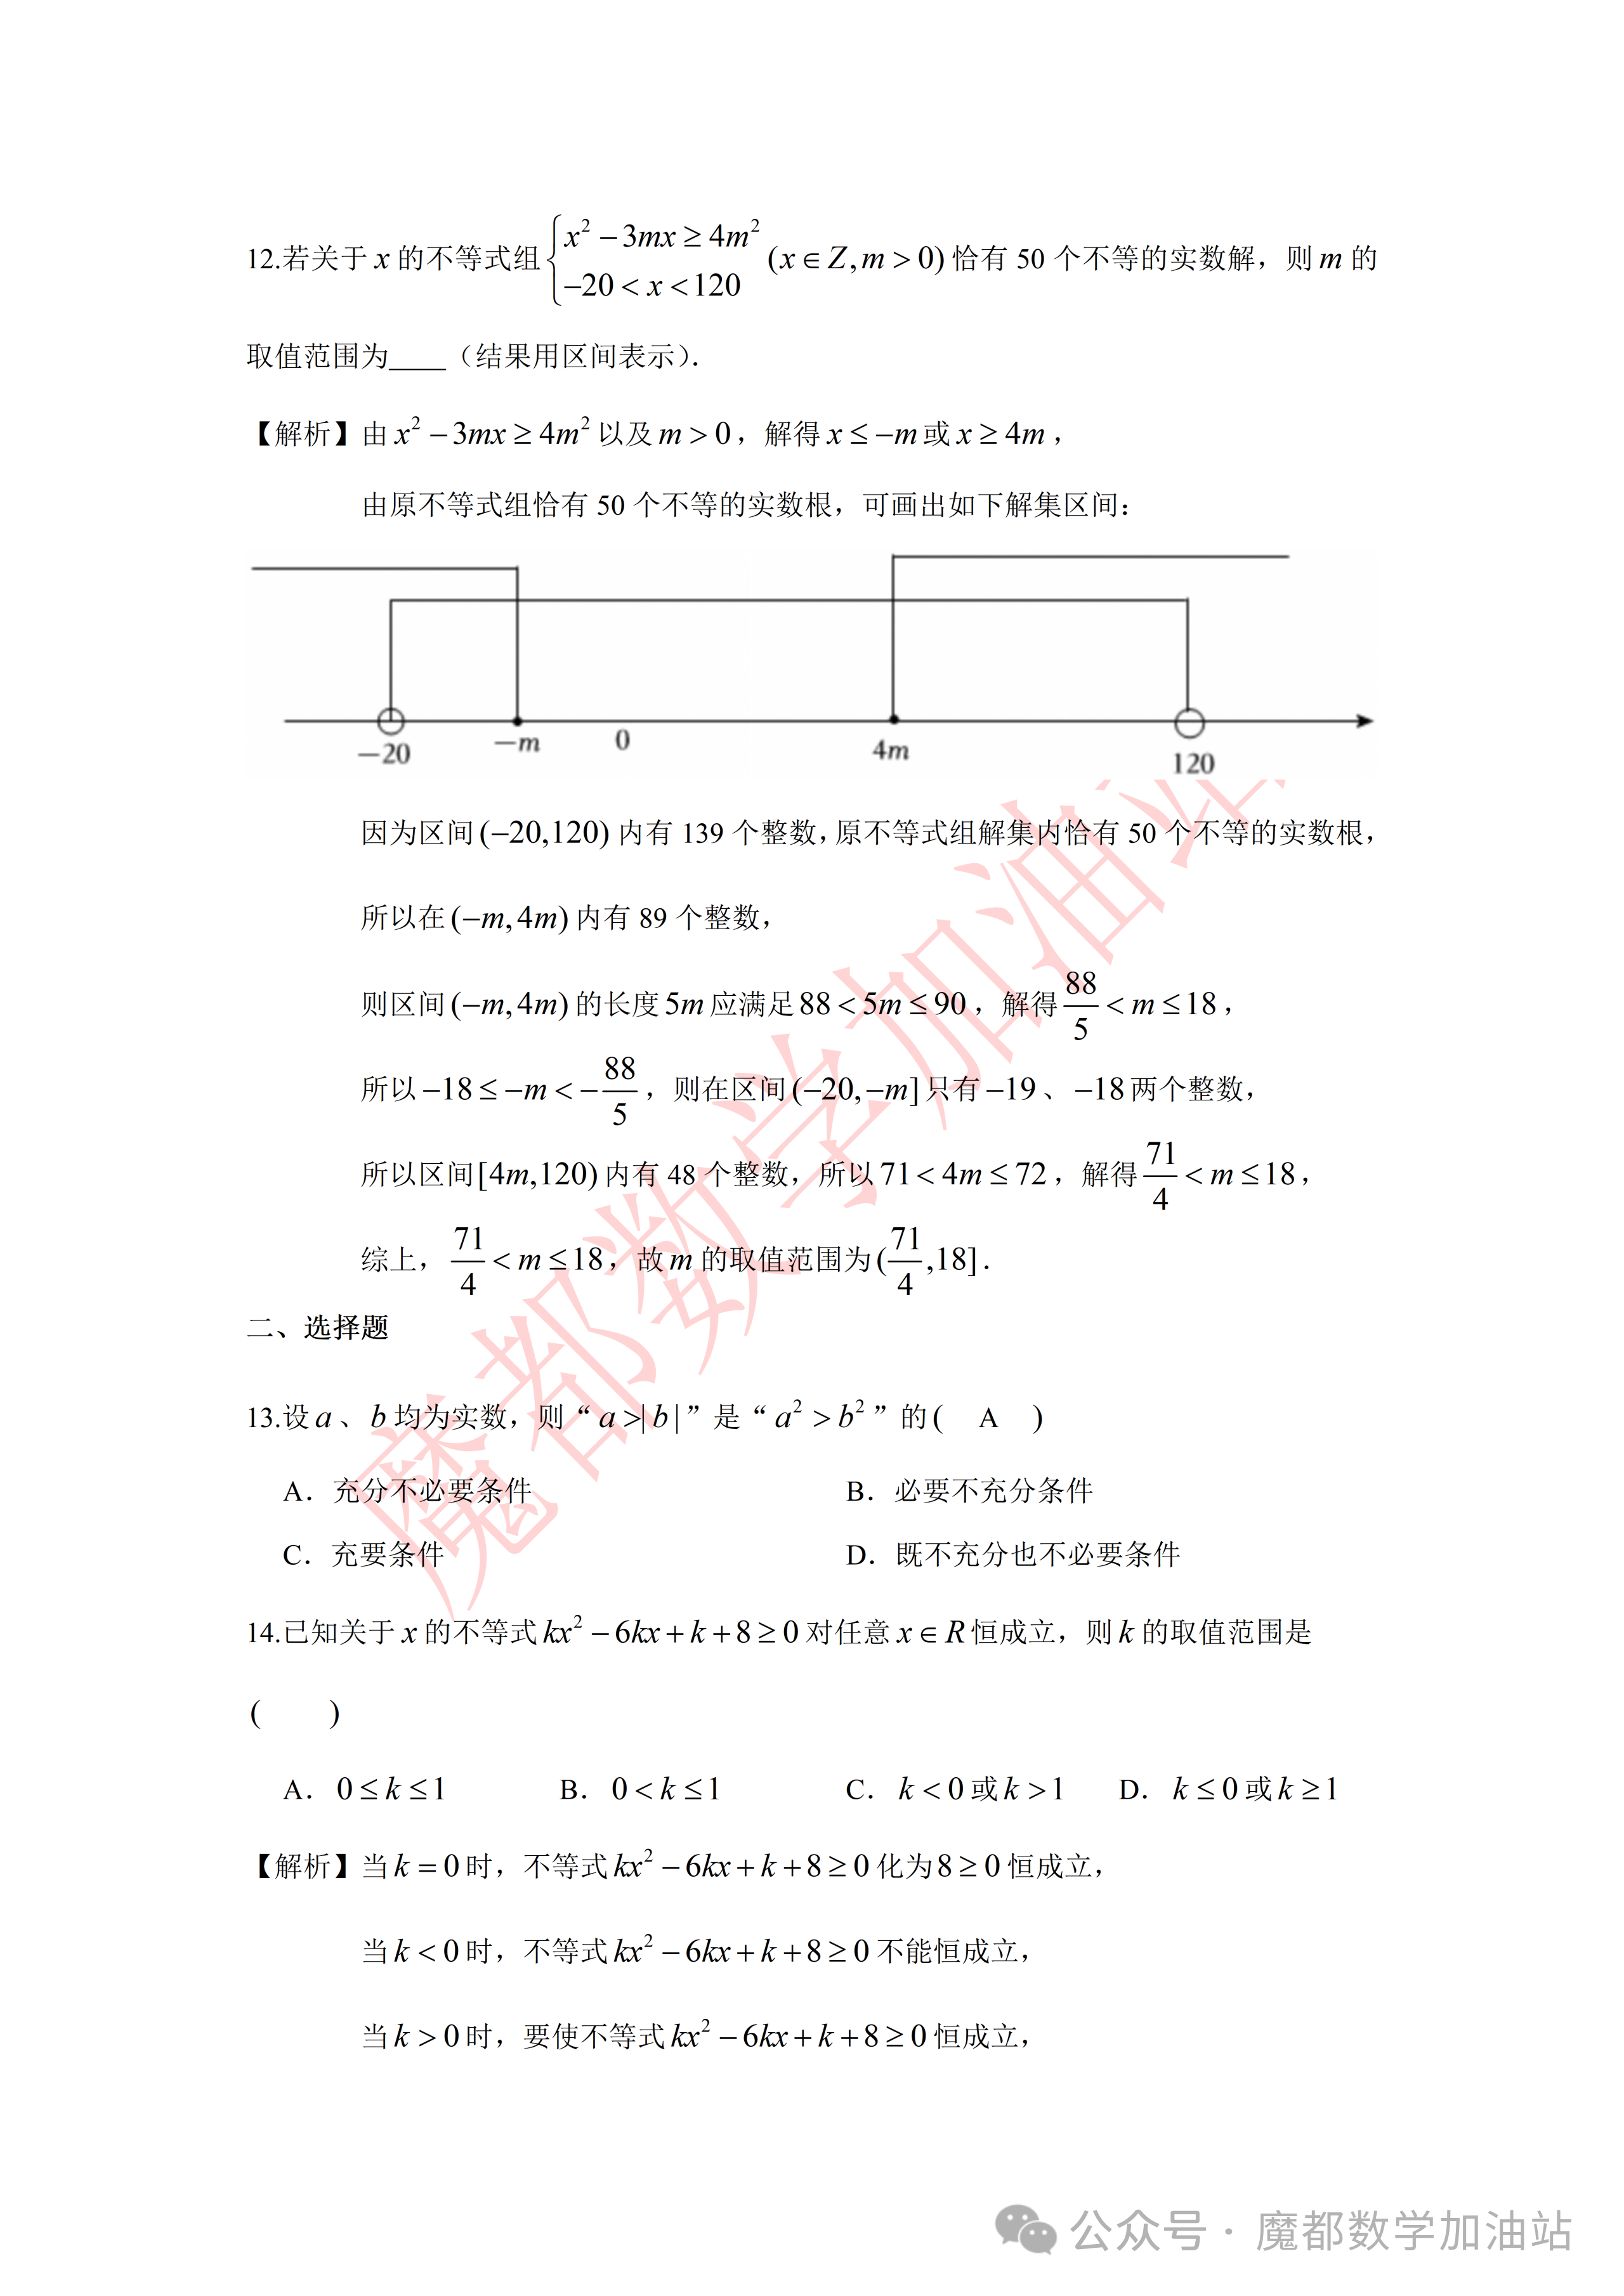
\includegraphics[width=.88\linewidth,trim=400bp 2410bp 320bp 860bp,clip]{../原图/高一46_交附闵行_国庆作业3/04.png}
\end{center}
\step{因为区间 $(-20,120)$ 内有 $139$ 个整数，原不等式组解集内有 $50$ 个不等的整数根，}
\step{所以在区间 $(-m,4m)$ 内有 $89$ 个整数，}
\step{则区间 $(-m,4m)$ 的长度 $5m$ 应满足 $88<5m\leqslant90$，解得 $\dfrac{88}{5}<m\leqslant18$，}
% 注：原卷题干称“实数解”，本行及后文按原卷解析照录为整数根计数。
\step{所以 $-18\leqslant-m<-\dfrac{88}{5}$，则在区间 $(-20,-m]$ 内有 $-19$、$-18$ 两个整数，}
\step{所以区间 $[4m,120)$ 内有 $48$ 个整数，}
\step{则 $71<4m\leqslant72$，解得 $\dfrac{71}{4}<m\leqslant18$，}
\step{综上，$\dfrac{71}{4}<m\leqslant18$，故 $m$ 的取值范围为 $\left(\dfrac{71}{4},18\right]$.}
\solend
\fi

\end{enumerate}

\bigsec{二、选择题}

\begin{enumerate}
\setcounter{enumi}{12}

\item 设 $a$、$b$ 均为实数，则“$a>|b|$”是“$a^2>b^2$”的\mbox{（\quad）}

\keepwithprev
A. 充分不必要条件\qquad B. 必要不充分条件

C. 充要条件\qquad\qquad D. 既不充分也不必要条件

\ans{$A$}

\item 已知关于 $x$ 的不等式 $kx^2-6kx+k+8\geqslant0$ 对任意 $x\in\R$ 恒成立，则 $k$ 的取值范围是\mbox{（\quad）}

\keepwithprev
A. $0\leqslant k\leqslant1$\qquad B. $0<k\leqslant1$

C. $k<0$ 或 $k>1$\qquad D. $k\leqslant0$ 或 $k\geqslant1$

\ans{$A$}

\ifanswer
\solbegin
\step{当 $k=0$ 时，不等式 $kx^2-6kx+k+8\geqslant0$ 化为 $8\geqslant0$ 恒成立，}
\step{当 $k<0$ 时，不等式 $kx^2-6kx+k+8\geqslant0$ 不能恒成立，}
\step{当 $k>0$ 时，要使不等式 $kx^2-6kx+k+8\geqslant0$ 恒成立，}
\step{需 $\Delta=36k^2-4(k^2+8k)\leqslant0$，解得 $0\leqslant k\leqslant1$，故选 $A$.}
\solend
\fi

\item 已知关于 $x$ 的不等式 $a\leqslant\dfrac34x^2-3x+4\leqslant b$，下列结论正确的是\mbox{（\quad）}

\keepwithprev
A. 当 $a<b<1$ 时，不等式 $a\leqslant\dfrac34x^2-3x+4\leqslant b$ 的解集非空

B. 当 $a=2$ 时，不等式 $a\leqslant\dfrac34x^2-3x+4\leqslant b$ 的解集可以为 $\{x\mid c\leqslant x\leqslant d\}$ 的形式

C. 不等式 $a\leqslant\dfrac34x^2-3x+4\leqslant b$ 的解集恰好为 $\{x\mid a\leqslant x\leqslant b\}$，那么 $b=\dfrac43$

D. 不等式 $a\leqslant\dfrac34x^2-3x+4\leqslant b$ 的解集恰好为 $\{x\mid a\leqslant x\leqslant b\}$，那么 $b-a=4$

\ans{$D$}

\ifanswer
\solbegin
\step{由 $\dfrac34x^2-3x+4\leqslant b$，得 $3x^2-12x+16-4b\leqslant0$，又 $b<1$，}
\step{所以 $\Delta=144-12(16-4b)=48(b-1)<0$，从而不等式无解，故 $A$ 错误；}
\step{在同一平面直角坐标系中作出函数 $y=\dfrac34x^2-3x+4=\dfrac34(x-2)^2+1$ 的图象及直线 $y=a$ 和 $y=b$，如图所示.}
\begin{center}
% 原图第 5 页解析配图直接裁取。
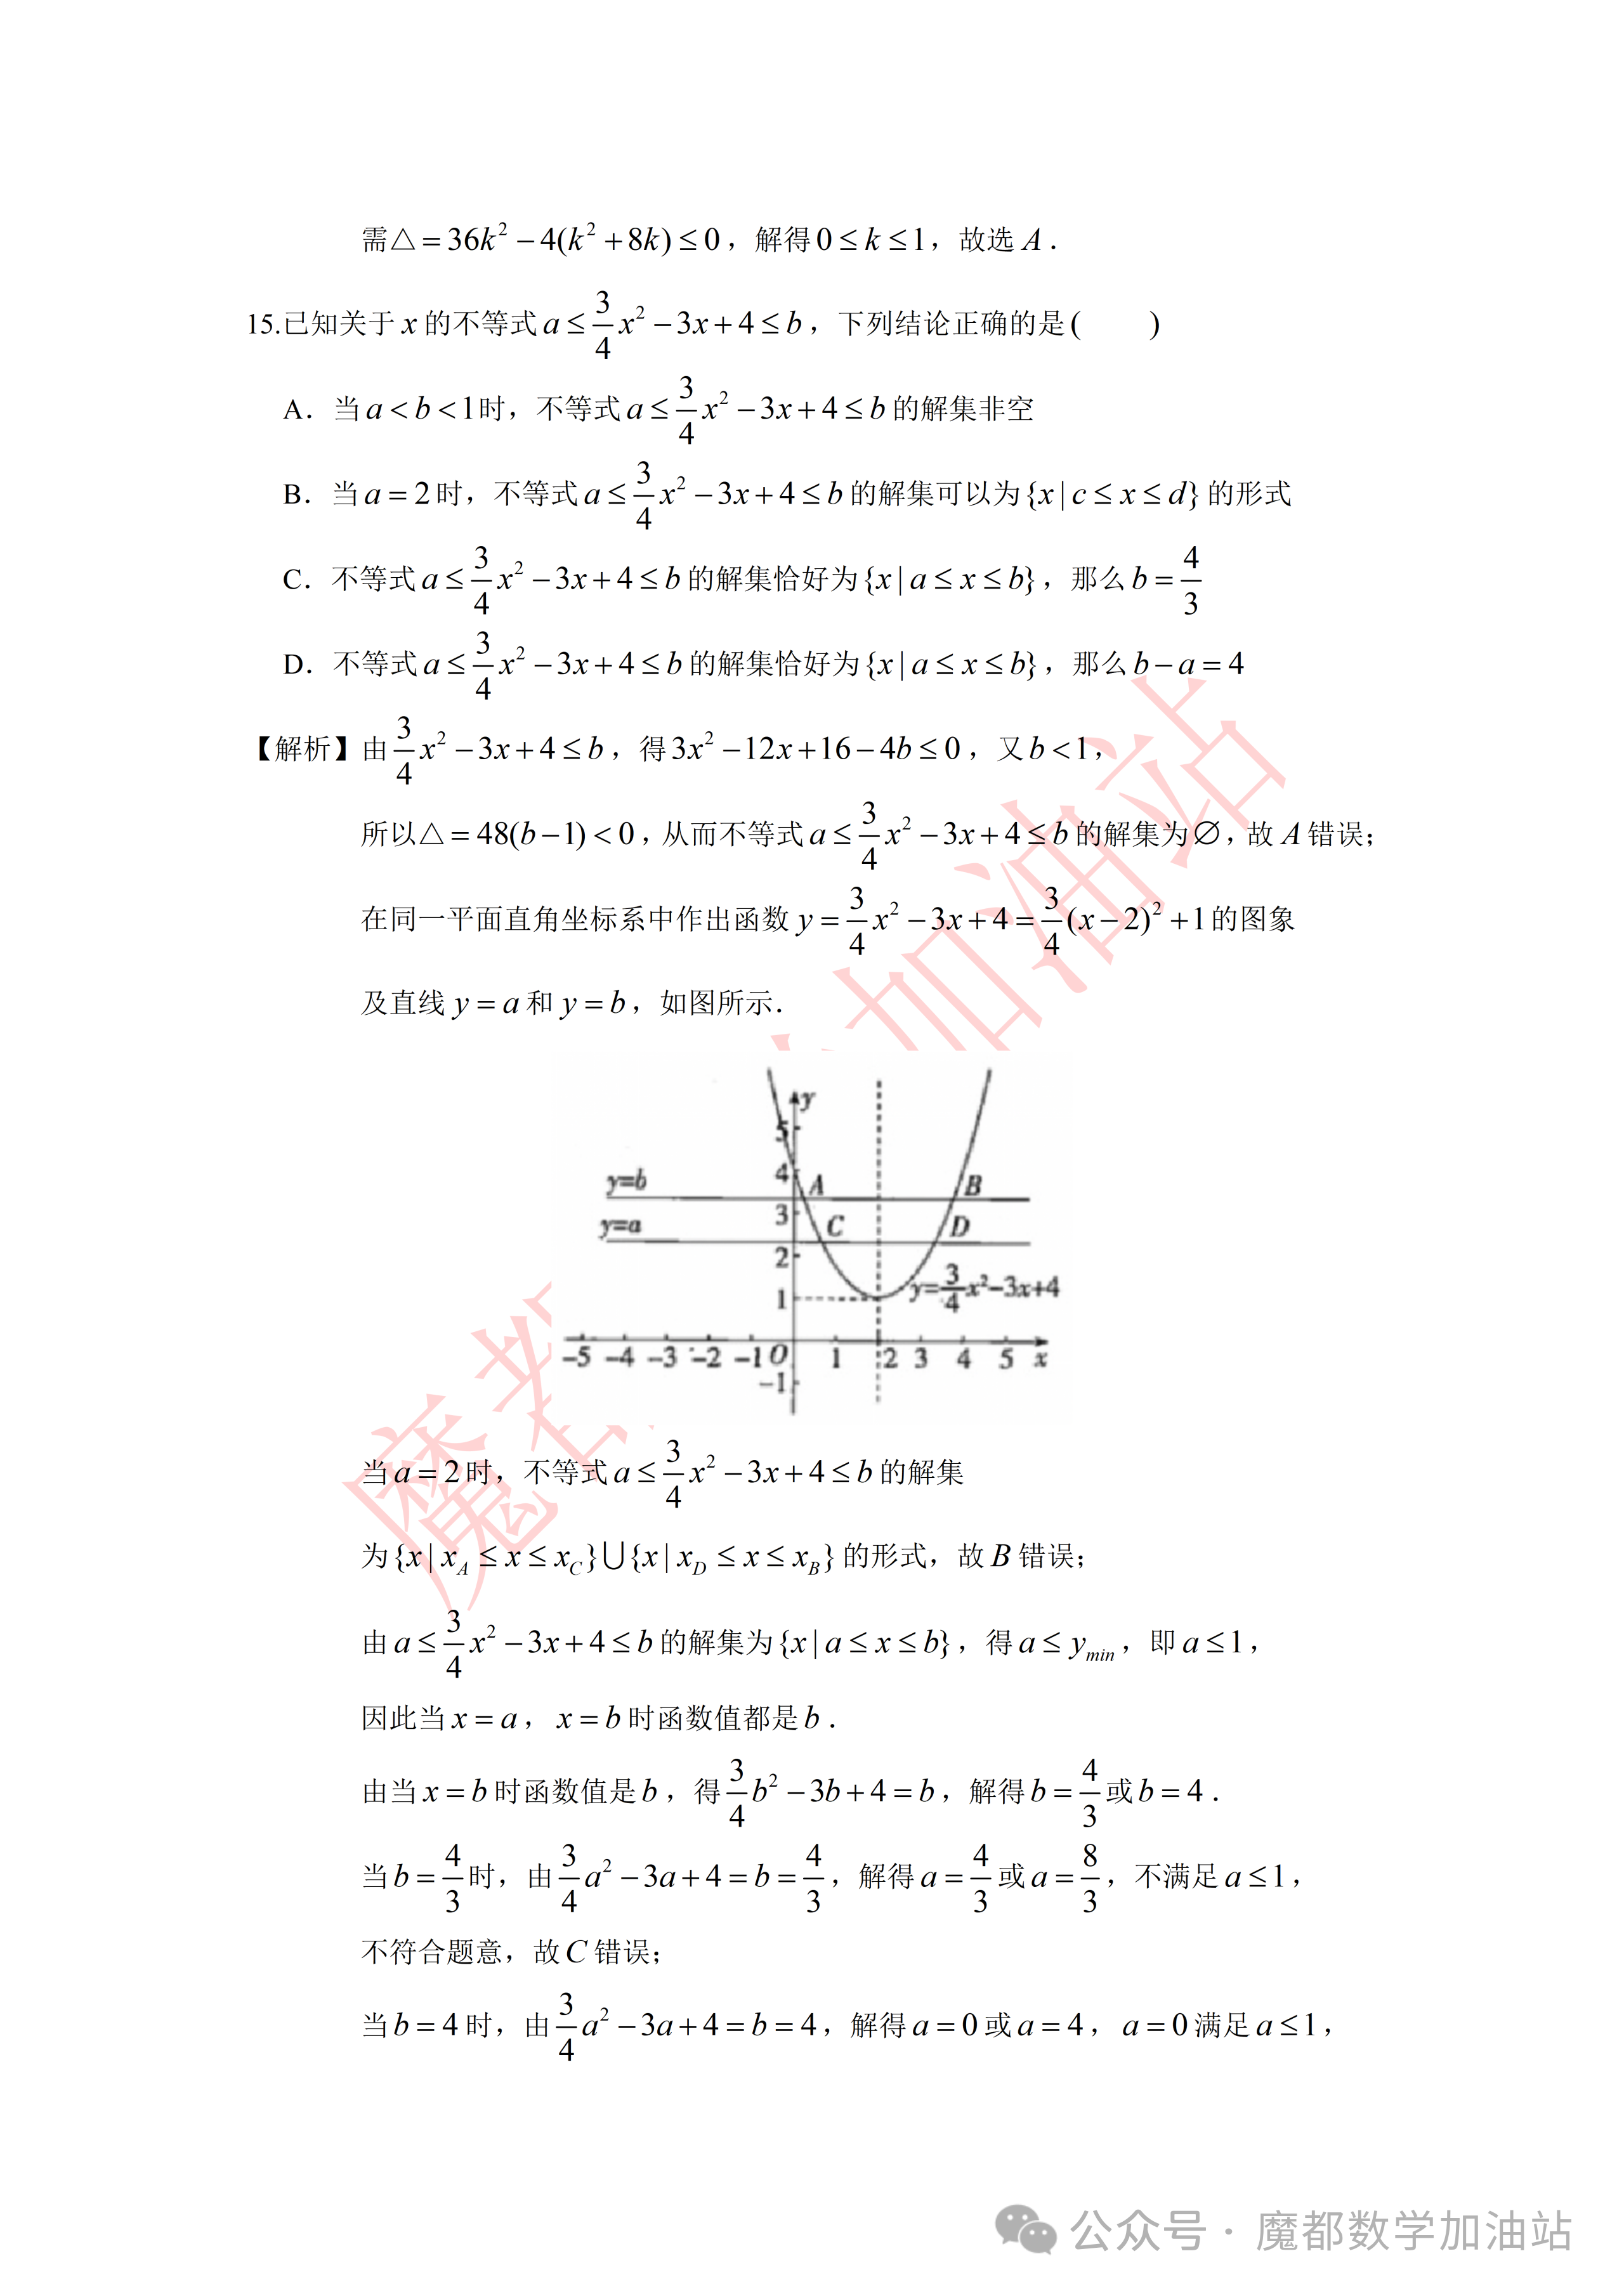
\includegraphics[width=.55\linewidth,trim=900bp 1400bp 760bp 1680bp,clip]{../原图/高一46_交附闵行_国庆作业3/05.png}
\end{center}
\step{当 $a=2$ 时，不等式 $a\leqslant\dfrac34x^2-3x+4\leqslant b$ 的解集为
$\{x\mid x_A\leqslant x\leqslant x_C\}\cup\{x\mid x_D\leqslant x\leqslant x_B\}$ 的形式，故 $B$ 错误；}
\step{由 $a\leqslant\dfrac34x^2-3x+4\leqslant b$ 的解集恰好为 $\{x\mid a\leqslant x\leqslant b\}$ 的形式，得 $a\leqslant y_{\min}$，即 $a\leqslant1$，}
\step{因为当 $x=a$、$x=b$ 时函数值都是 $b$，当 $x=a$ 时，$\dfrac34a^2-3a+4=b$；当 $x=b$ 时，$\dfrac34b^2-3b+4=b$，}
\step{解得 $b=\dfrac43$ 或 $b=4$，}
\step{当 $b=\dfrac43$ 时，由 $\dfrac34a^2-3a+4=b$，解得 $a=\dfrac43$ 或 $a=\dfrac83$，不符合题意，故 $C$ 错误；}
\step{当 $b=4$ 时，由 $\dfrac34a^2-3a+4=b$，解得 $a=0$ 或 $a=4$，$a=0$ 满足 $a\leqslant1$，故 $D$ 正确；}
\step{故选 $D$.}
\solend
\fi

\item 已知 $x$、$y\in(0,+\infty)$，则 $(x-y)^2+2y+1-x+\dfrac4x$ 的最小值为\mbox{（\quad）}

\keepwithprev
A. $1$\qquad B. $2$\qquad C. $3$\qquad D. $4$

\ans{$D$}

\ifanswer
\solbegin
\step{因为 $(x-y)^2+2y+1-x+\dfrac4x=(x-y-1)^2+x+\dfrac4x$，}
\step{当且仅当 $x-y-1=0$，且 $x=\dfrac4x$ 时取等号，}
\step{又因为 $x+\dfrac4x\geqslant2\sqrt{x\cdot\dfrac4x}=4$，当且仅当 $x=2$ 时取等号，}
\step{故选 $D$.}
\solend
\fi

\end{enumerate}

\bigsec{三、解答题}

\begin{enumerate}
\setcounter{enumi}{16}

\item 设集合 $A=\left\{x\middle|\dfrac{x-3}{x-1}<0\right\}$，$B=\{x\mid x^2-2ax+a^2-1>0\}$.
\begin{enumerate}[label=(\arabic*)]
\item 若 $a=3$，求 $A\cup B$；
\item 若“$x\in A$”是“$x\in B$”的充分条件，求实数 $a$ 的取值范围.
\end{enumerate}

\ifanswer
\solbegin
% 注：原卷题干为 a^2-1，故 a=3 时常数项为 8；题干与本步一致。
\stepm{(1)}{当 $a=3$ 时，$B=\{x\mid x^2-6x+8>0\}=\{x\mid x<2\text{ 或 }x>4\}$；}
\step{因为 $A=\left\{x\middle|\dfrac{x-3}{x-1}<0\right\}=\{x\mid(x-1)(x-3)<0\}=\{x\mid1<x<3\}$，}
\step{所以 $A\cup B=\{x\mid x<2\text{ 或 }x>4\}\cup\{x\mid1<x<3\}
=\{x\mid x<3\text{ 或 }x>4\}$.}
\stepm{(2)}{因为“$x\in A$”是“$x\in B$”的充分条件，所以 $A\subseteq B$，}
\step{因 $A=\left\{x\middle|\dfrac{x-3}{x-1}<0\right\}
=\{x\mid(x-1)(x-3)<0\}=\{x\mid1<x<3\}$，}
\step{所以 $A\subseteq B=\{x\mid x<a-1\text{ 或 }x>a+1\}$，}
\step{要使 $A\subseteq B$，需有 $a-1\geqslant3$ 或 $a+1\leqslant1$，}
\step{所以 $a\geqslant4$ 或 $a\leqslant0$，故 $a$ 的取值范围为 $\{a\mid a\geqslant4\text{ 或 }a\leqslant0\}$.}
\solend
\fi

\ansspace[6]

\item 某学校引入种植类劳动教育课程，打算围成如图所示的四块全等的长方形田地种植不同种类的蔬菜，其中一面可以利用原有的墙（足够长），其他各面需要用篱笆围成，设其中一块田地为矩形 $ABCD$.

\begin{center}
% 原图第 6 页配图直接裁取。
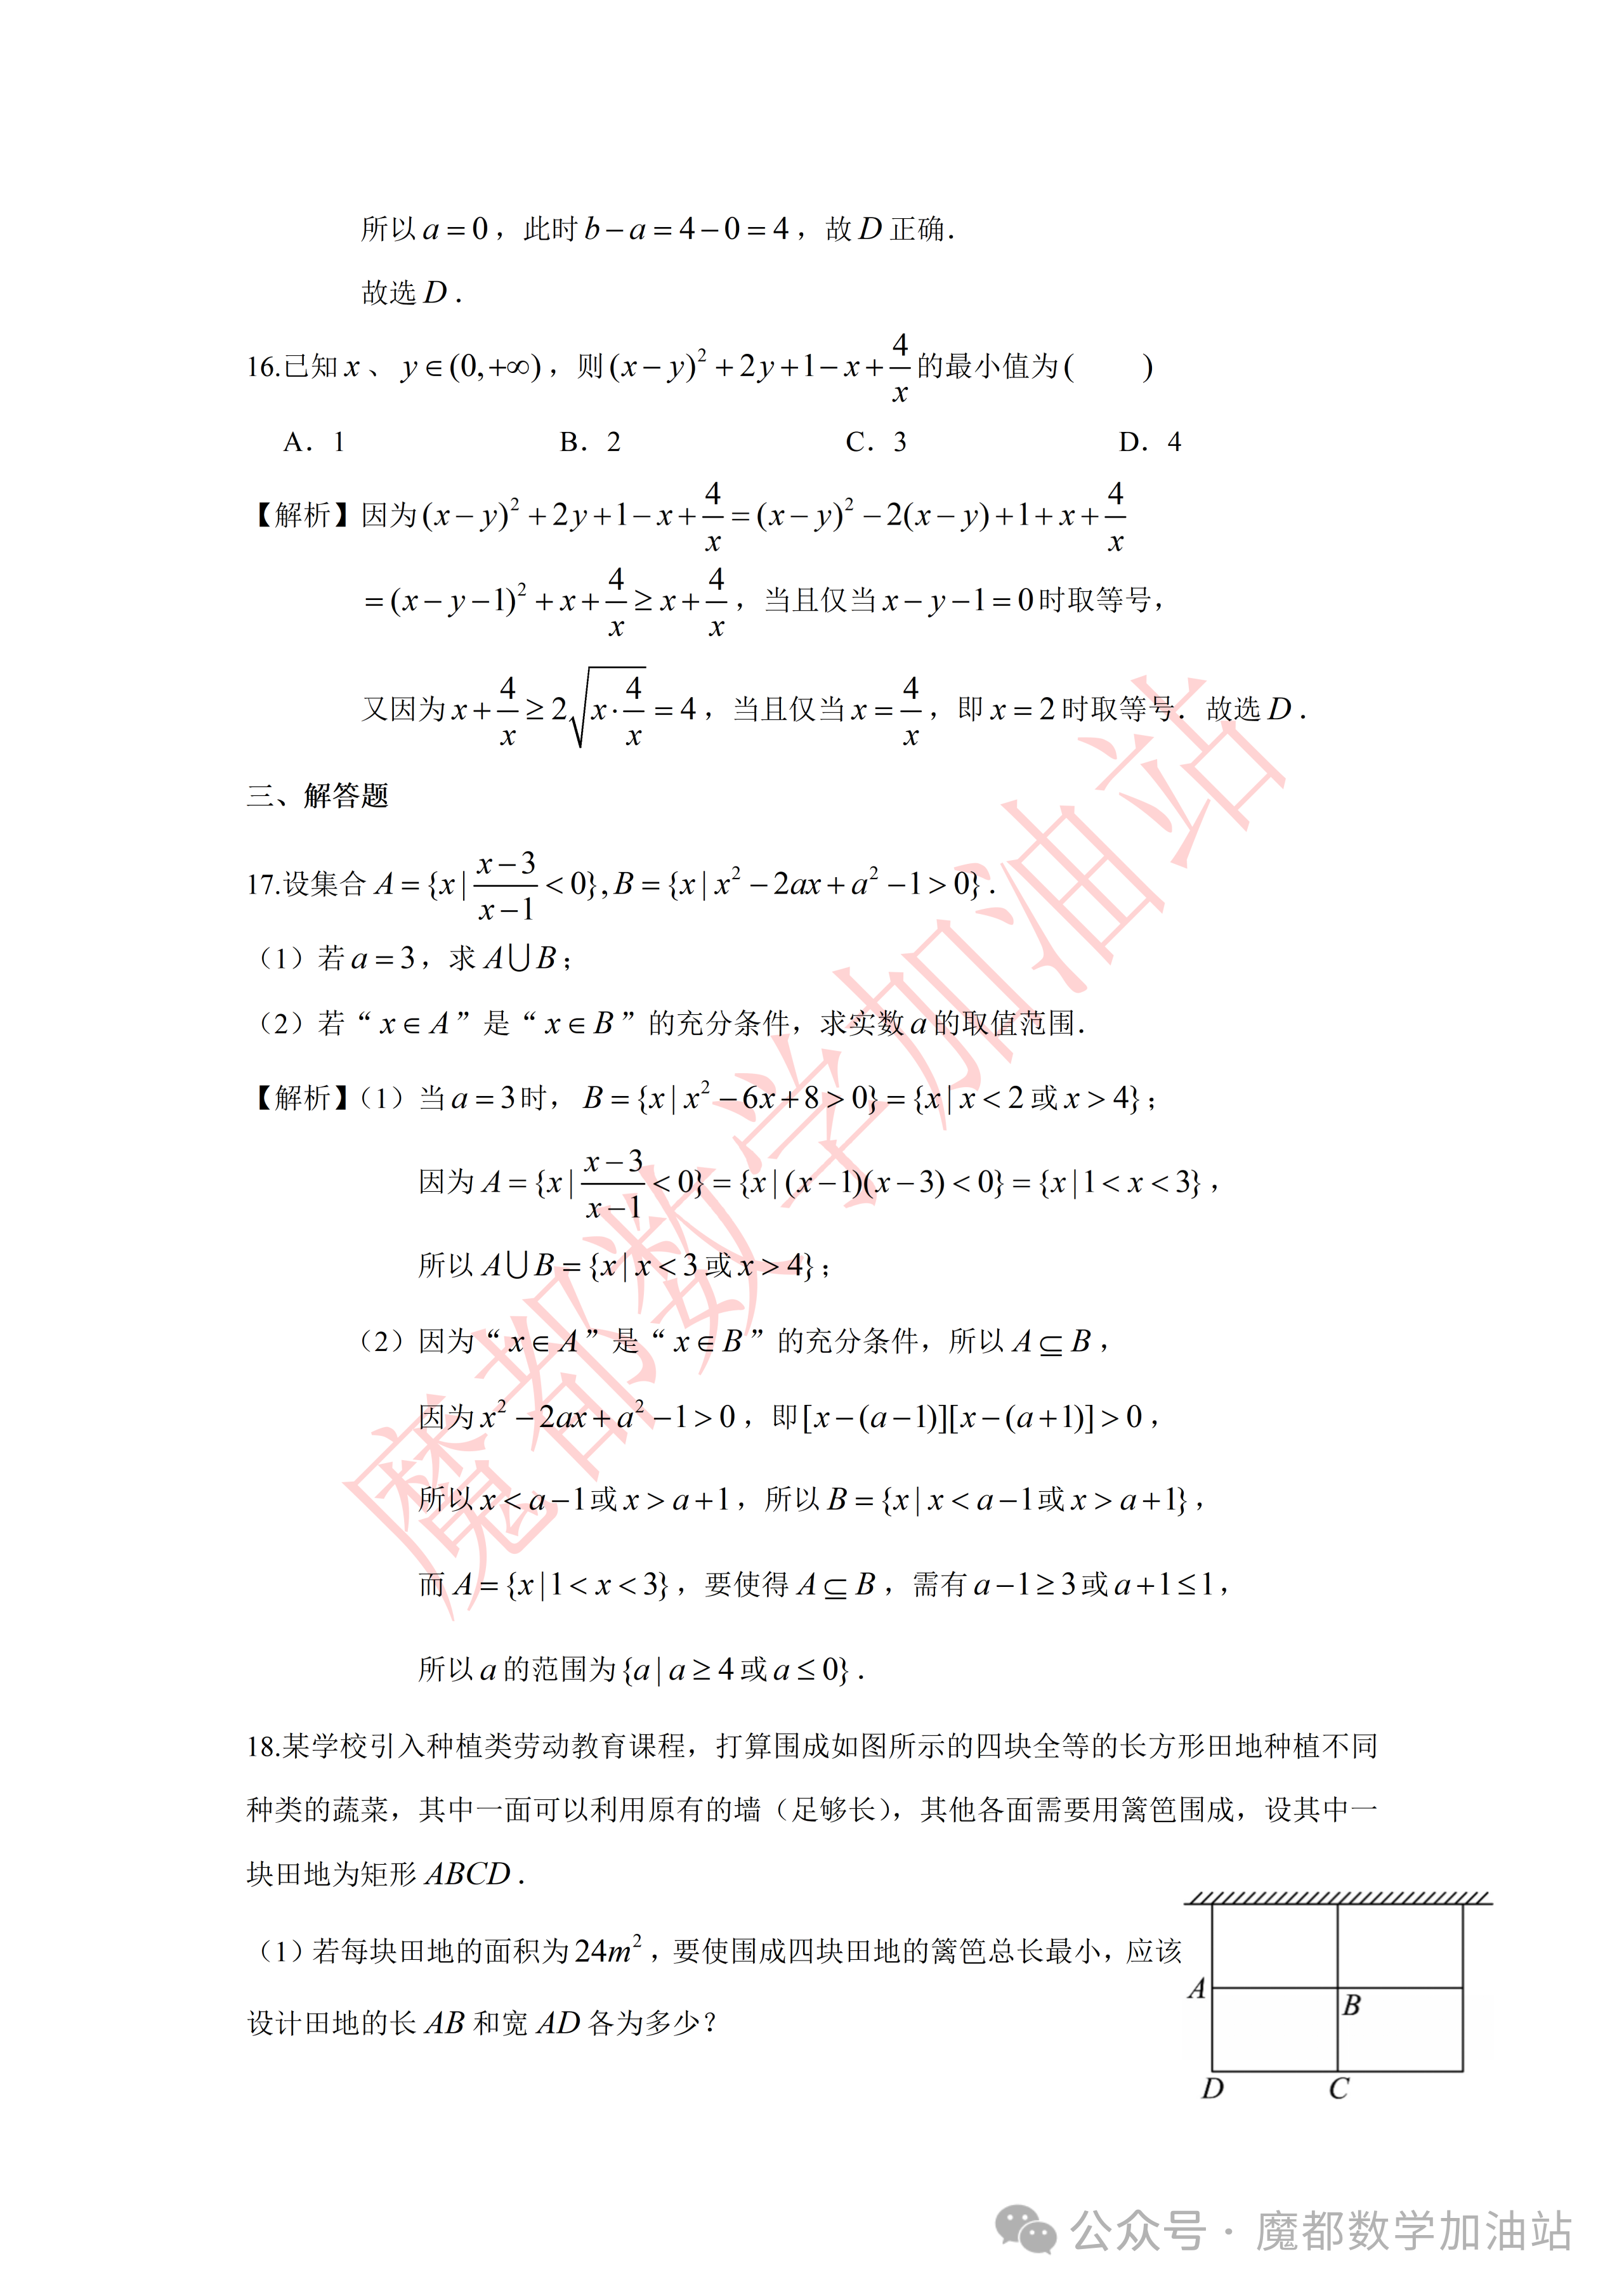
\includegraphics[width=.33\linewidth,trim=1866bp 220bp 210bp 2960bp,clip]{../原图/高一46_交附闵行_国庆作业3/06.png}
\end{center}

\begin{enumerate}[label=(\arabic*)]
\item 若每块田地的面积为 $24\,\text{m}^2$，要使围成四块田地的篱笆总长最小，应该设计田地的长 $AB$ 和宽 $AD$ 各为多少？
\item 现有 $40\,\text{m}$ 长的篱笆，要使每块田地的面积最大，应该设计田地的长 $AB$ 和宽 $AD$ 各为多少？
\end{enumerate}

\ifanswer
\solbegin
\stepm{(1)}{设 $AB$ 长为 $x\,\text{m}$，$AD$ 宽为 $y\,\text{m}$，由题意得 $xy=24$，篱笆总长为 $4x+6y$，}
\step{$4x+6y\geqslant2\sqrt{4x\cdot6y}=2\sqrt{24xy}=48$，}
\step{当且仅当 $4x=6y$ 时取等号，解得 $x=6$，$y=4$，}
\step{所以田地的长 $AB$ 为 $6\,\text{m}$，宽 $AD$ 为 $4\,\text{m}$.}
\stepm{(2)}{设 $AB$ 长为 $a\,\text{m}$，$AD$ 宽为 $b\,\text{m}$，由篱笆总长 $4a+6b=40$，即 $2a+3b=20$，}
\step{将 $a=\dfrac{20-3b}{2}$ 代入每块田地面积 $ab$，得 $ab=\dfrac12b(20-3b)=-\dfrac32b^2+10b$，}
\step{当 $b=\dfrac{10}{3}$ 时，$ab$ 最大，此时 $a=5$，}
\step{所以田地的长 $AB$ 为 $5\,\text{m}$，宽 $AD$ 为 $\dfrac{10}{3}\,\text{m}$.}
\solend
\fi

\ansspace[8]

\item 已知 $x_1$、$x_2$ 是一元二次方程 $4kx^2-4kx+k+1=0$ 的两个不等实数根.
\begin{enumerate}[label=(\arabic*)]
\item 若 $x_1$、$x_2$ 均为正根，求实数 $k$ 的取值范围；
\item 求使 $\dfrac{x_1}{x_2}+\dfrac{x_2}{x_1}-2$ 的值为整数 $k$ 的整数值.
\end{enumerate}

\ifanswer
\solbegin
\stepm{(1)}{由题意，$x_1$、$x_2$ 是方程 $4kx^2-4kx+k+1=0$ 的两个不等实数根，}
\step{故 $k\neq0$，$\Delta=(-4k)^2-16k(k+1)>0$，得 $-16k>0$，所以 $k<0$，}
\step{又 $x_1+x_2=1$，$x_1x_2=\dfrac{k+1}{4k}>0$，得 $k+1<0$，}
\step{所以 $k$ 的取值范围为 $(-\infty,-1)$.}
\stepm{(2)}{由题意，}
\step{$\dfrac{x_1}{x_2}+\dfrac{x_2}{x_1}-2
=\dfrac{x_1^2+x_2^2-2x_1x_2}{x_1x_2}
=\dfrac{(x_1+x_2)^2-4x_1x_2}{x_1x_2}$，}
\step{又 $x_1+x_2=1$，$x_1x_2=\dfrac{k+1}{4k}$，}
\step{则 $\dfrac{x_1}{x_2}+\dfrac{x_2}{x_1}-2=-\dfrac4{k+1}$，}
\step{由于 $-\dfrac4{k+1}$ 为整数，故 $k+1$ 只能取 $\pm1$、$\pm2$、$\pm4$，又 $k<-1$，}
\step{所以整数 $k$ 的值为 $-2$、$-3$、$-5$.}
\solend
\fi

\ansspace[8]

\item 已知 $a>0$，$b>0$，且 $2a+3b=3$.
\begin{enumerate}[label=(\arabic*)]
\item 求 $ab$ 的最大值；
\item 求 $a-\dfrac1{6b}$ 的最大值；
\item 求 $\dfrac2a+\dfrac3{b+1}$ 的最小值.
\end{enumerate}

\ifanswer
\solbegin
\stepm{(1)}{由 $2a+3b=3$，得 $3=2a+3b\geqslant2\sqrt{6ab}$，}
\step{所以 $ab\leqslant\dfrac38$，当且仅当 $2a=3b=\dfrac32$ 时取等号，}
\step{故 $ab$ 的最大值为 $\dfrac38$.}
\stepm{(2)}{由 $2a+3b=3$，得 $a=\dfrac32-\dfrac32b$，}
\step{则 $a-\dfrac1{6b}=\dfrac32-\dfrac32b-\dfrac1{6b}$，}
\step{由基本不等式，$\dfrac32b+\dfrac1{6b}\geqslant2\sqrt{\dfrac32b\cdot\dfrac1{6b}}=1$，}
\step{当且仅当 $\dfrac32b=\dfrac1{6b}$，即 $b=\dfrac13$、$a=1$ 时取等号，}
\step{所以 $a-\dfrac1{6b}$ 的最大值为 $\dfrac12$.}
\stepm{(3)}{由 $2a+3b=3$，得 $2a+3(b+1)=6$，}
\step{$\dfrac2a+\dfrac3{b+1}
=\dfrac16\left(2a+3(b+1)\right)\left(\dfrac2a+\dfrac3{b+1}\right)$}
\step{$=\dfrac16\left(13+\dfrac{6(b+1)}a+\dfrac{6a}{b+1}\right)
\geqslant\dfrac16\left(13+2\sqrt{\dfrac{6(b+1)}a\cdot\dfrac{6a}{b+1}}\right)=\dfrac{25}{6}$，}
\step{当且仅当 $a=b+1$，即 $a=\dfrac65$、$b=\dfrac15$ 时取等号，}
\step{所以 $\dfrac2a+\dfrac3{b+1}$ 的最小值为 $\dfrac{25}{6}$.}
\solend
\fi

\ansspace[8]

\item 已知 $U=\R$ 为全集，集合 $A=\{s^2+3t^2\mid s,t\in U\}$.
\begin{enumerate}[label=(\arabic*)]
\item 设 $U=\{1,3,5\}$，求集合 $A$ 的元素个数；
\item 设 $U=\Z$，证明：若 $x\in A$，则 $7x\in A$；
\item 设 $U=\R$，$x$、$y\in A$，且 $x=m^2+3n^2$，$y=p^2+3q^2$，若 $mp-3nq=\sqrt3$，求 $x+y+mq+np$ 的最小值.
\end{enumerate}

\ifanswer
\solbegin
\stepm{(1)}{当 $s=1$，$t=1$ 时，$s^2+3t^2=1+3=4$；}
\step{当 $s=1$，$t=3$ 时，$s^2+3t^2=1+27=28$；}
\step{当 $s=1$，$t=5$ 时，$s^2+3t^2=1+75=76$；}
\step{当 $s=3$，$t=1$ 时，$s^2+3t^2=9+3=12$；}
\step{当 $s=3$，$t=3$ 时，$s^2+3t^2=9+27=36$；}
\step{当 $s=3$，$t=5$ 时，$s^2+3t^2=9+75=84$；}
\step{当 $s=5$，$t=1$ 时，$s^2+3t^2=25+3=28$；}
\step{当 $s=5$，$t=3$ 时，$s^2+3t^2=25+27=52$；}
\step{当 $s=5$，$t=5$ 时，$s^2+3t^2=25+75=100$，}
\step{所以 $A=\{4,12,28,36,52,76,84,100\}$，有 $8$ 个元素.}
\stepm{(2)}{因为 $U=\Z$，$x\in A$，设 $x=s^2+3t^2$，}
\step{则 $7x=7(s^2+3t^2)=(2s+3t)^2+3(s-2t)^2\in A$，}
\step{所以 $7x\in A$.}
\stepm{(3)}{因为 $x=m^2+3n^2$，$y=p^2+3q^2$，}
\step{$xy=(m^2+3n^2)(p^2+3q^2)=3(mq+np)^2+(mp-3nq)^2$，}
\step{设 $mq+np=b$，则 $xy=3b^2+3$，所以 $y=\dfrac{3b^2+3}{x}$，}
\step{于是 $x+y+mq+np=x+\dfrac{3b^2+3}{x}+b\geqslant2\sqrt{3b^2+3}+b$，}
\step{设 $2\sqrt{3b^2+3}+b=t$，整理得 $11b^2+2bt+12-t^2=0$，}
\step{判别式法，$\Delta=4t^2-44(12-t^2)\geqslant0$，得 $t\geqslant\sqrt{11}$，}
\step{即 $(x+y+mq+np)_{\min}=\sqrt{11}$，所以 $x+y+mq+np$ 的最小值为 $\sqrt{11}$.}
\solend
\fi

\ansspace*[10]

\end{enumerate}

\end{document}
"
%
% 原始材料：微信公众号“魔都数学加油站”，作者破晓，2026-10-02 17:56 发布。
% 原文标题：“27学年高一46——2026-2027你那上海市交附闵行高一上国庆作业3”
% （公众号标题中的“你那”照录，系原文标题字样）；原文链接：
% http://mp.weixin.qq.com/s?__biz=Mzg4ODU1ODMxOQ==&mid=2247591657&idx=3&sn=a894d1a16611283a61b3eaba32a3f24c&chksm=cee83366c6a55381b370069f84ef63d20251f94608bb37cc4ec2d66227401bd147f4f6bd8256&scene=126&sessionid=1790935402&subscene=7&clicktime=1790937618&enterid=1790937618#rd
% 正文为 9 张 PNG 页，按页序读取原图；第 01、02、07 页 4762×6735，
% 第 03—06、08、09 页 2560×3620。卷面标题照原卷印作“2026-2027 年交附闵行高一上国庆作业 3”。
% 原文从第 3 题起，题号照原卷保留；正文为讲评版，答案、解析依原卷顺序录入。
% 水印及页脚公众号标识不录入。卷面插图直接裁取对应原图页，不另制图片文件。
%
% 与原卷的排版差异：
%   ① 原卷按“一、填空题”“二、选择题”“三、解答题”分节，本稿沿用原节与原题号，
%      只改排为全稿统一的大节样式；
%   ② 原卷答案与解析依页面位置分布，本稿按 common.sty 统一置于答案版；
%   ③ 原卷副标题未印，本稿按“知识模块”口径标作“集合与常用逻辑用语、不等式”。
%
% 原卷存疑一处（照抄未改，见第 12 题题干及解析处注释）：
%   第 12 题题干同时给出 x∈Z，却称不等式组有“50 个不等的实数解”；解析按整数根计数。
%   此处题干与解析的原文不一致，本稿均照录。
% 第 17 题曾疑似有常数项不一致：复核原图题干为 a^2-1，a=3 时常数项确为 8，
% 与解析相符；不将其记作原卷错误。
%
\documentclass[a4paper,11pt]{article}
\usepackage{common}

\begin{document}

\examtitlest[3]{2026--2027 年交附闵行高一上国庆作业 3}{集合与常用逻辑用语、不等式}

\bigsec{一、填空题}

\begin{enumerate}
\setcounter{enumi}{2}

\item 不等式 $\dfrac{x^2-10}{x+2}\geqslant1$ 的解集为\blankline[4.4em].

\ifanswer
\ans{$\{x\mid-3\leqslant x<-2\text{ 或 }x\geqslant4\}$}
\solbegin
\step{不等式 $\dfrac{x^2-10}{x+2}\geqslant1$，移项得 $\dfrac{x^2-10}{x+2}-1\geqslant0$，}
\step{通分得 $\dfrac{x^2-x-12}{x+2}\geqslant0$，即 $\dfrac{(x-4)(x+3)}{x+2}\geqslant0$，}
\step{解得 $-3\leqslant x<-2$ 或 $x\geqslant4$，}
\step{故不等式的解集为 $\{x\mid-3\leqslant x<-2\text{ 或 }x\geqslant4\}$.}
\solend
\fi

\item $|x-3|+|x-5|\geqslant2$，当等号成立时，$x$ 的范围是\blankline[4.4em].

\ifanswer
\ans{$[3,5]$}
\fi

\item 若直角三角形斜边长等于 $4\sqrt2\,\text{cm}$，则直角三角形面积的最大值为\blankline[4.4em].

\ifanswer
\solbegin
\step{设 $Rt\triangle ABC$ 中，$C=90^\circ$，则 $c=\sqrt{a^2+b^2}=4\sqrt2$，所以 $a^2+b^2=32$，}
\step{由基本不等式得 $a^2+b^2\geqslant2ab$，当且仅当 $a=b=4$ 时取等号，}
\step{所以 $\triangle ABC$ 的面积 $S=\dfrac12ab\leqslant8$，}
\step{当且仅当 $a=b=4$ 时，$\triangle ABC$ 的面积最大值为 $8$.}
\solend
\fi

\item 不等式 $(x-1)(2-x)>0$ 的解集为\blankline[4.4em].

\ifanswer
\solbegin
\step{$(x-1)(2-x)>0\Rightarrow(x-1)(x-2)<0$，}
\step{故不等式的解集为 $\{x\mid1<x<2\}$.}
\solend
\fi

\item 已知集合 $A=\{1,2\}$，$B=\{x\mid x^2-2mx+m=0\}$，$A\cup B=A$，则实数 $m$ 的取值范围为\blankline[4.4em].

\ifanswer
\solbegin
\step{因为 $A\cup B=A$，所以 $B\subseteq A$，}
\step{当 $B=\varnothing$ 时，$\Delta=(-2m)^2-4m<0$，解得 $0<m<1$，}
\step{当 $B$ 为单元素集时，$\Delta=0$，解得 $m=0$ 或 $m=1$，}
\step{当 $m=0$ 时，方程 $x^2=0$，解得 $x=0$，此时 $B=\{0\}$，不满足 $B\subseteq A$；}
\step{当 $m=1$ 时，方程 $x^2-2x+1=0$，解得 $x=1$，此时 $B=\{1\}$，满足 $B\subseteq A$；}
\step{当 $B=\{1,2\}$ 时，由韦达定理得 $1+2=2m$，$1\times2=m$，无解，}
\step{综上所述，实数 $m$ 的取值范围为 $\{m\mid0<m\leqslant1\}$.}
\solend
\fi

\item 设 $a$、$b$、$c\in\R^+$，若 $a+b+c=1$，则 $\dfrac1a+\dfrac1b+\dfrac1c\geqslant$\blankline[4.4em].

\ifanswer
\solbegin
\step{因为 $a$、$b$、$c\in\R^+$，且 $a+b+c=1$，}
\step{所以 $\dfrac1a+\dfrac1b+\dfrac1c=(a+b+c)\left(\dfrac1a+\dfrac1b+\dfrac1c\right)$}
\step{$=3+\dfrac ab+\dfrac ba+\dfrac ac+\dfrac ca+\dfrac bc+\dfrac cb$，}
\step{由基本不等式得 $\dfrac ab+\dfrac ba\geqslant2$，$\dfrac ac+\dfrac ca\geqslant2$，$\dfrac bc+\dfrac cb\geqslant2$，}
\step{所以 $\dfrac1a+\dfrac1b+\dfrac1c\geqslant9$，当且仅当 $a=b=c=\dfrac13$ 时取等号，}
\step{所以 $\dfrac1a+\dfrac1b+\dfrac1c$ 的最小值为 $9$.}
\solend
\fi

\item 已知 $-1\leqslant x+y\leqslant2$，$-2\leqslant x-y\leqslant1$，则 $x-2y$ 的范围为\blankline[4.4em].

\ifanswer
\solbegin
\step{设 $x-2y=m(x+y)+n(x-y)$，}
\step{则 $x-2y=(m+n)x+(m-n)y$，所以 $m+n=1$，$m-n=-2$，}
\step{解得 $m=-\dfrac12$，$n=\dfrac32$，}
\step{所以 $x-2y=-\dfrac12(x+y)+\dfrac32(x-y)$，}
\step{因为 $-1\leqslant x+y\leqslant2$，$-2\leqslant x-y\leqslant1$，}
\step{所以 $-4\leqslant x-2y\leqslant2$，即 $x-2y$ 的范围为 $[-4,2]$.}
\solend
\fi

\item 设集合 $A=\{1,2,m\}$，其中 $m$ 为实数，令 $B=\{a^2\mid a\in A\}$，$C=A\cup B$. 若 $C$ 中所有元素之和为 $6$，则 $C$ 中的所有元素之积为\blankline[4.4em].

\ifanswer
\solbegin
\step{因为 $A=\{1,2,m\}$，所以 $B=\{a^2\mid a\in A\}=\{1,4,m^2\}$，$m\neq1$，$m\neq2$，}
\step{又 $C=A\cup B$，所以 $1\in C$，$4\in C$，$m^2\in C$，}
\step{若 $m^2=1$，则 $m=-1$ 或 $m=1$（舍），当 $m=-1$ 时，$C=\{1,2,4,-1\}$，$C$ 中所有元素之和为 $6$，}
\step{此时 $C$ 中所有元素之积为 $-8$；}
\step{若 $m^2=2$，则 $m=-\sqrt2$ 或 $m=\sqrt2$，$C$ 中所有元素之和不符合题意；}
\step{若 $m^2=4$，则 $m=-2$ 或 $m=2$，此时 $C=\{1,2,4,-2\}$ 或 $C=\{1,2,4\}$，所有元素之和不符合题意；}
\step{若 $m^2\neq1$，$m^2\neq2$，$m^2\neq4$，则 $C=\{1,2,4,m,m^2\}$，}
\step{所以 $1+2+4+m+m^2=6$，即 $m^2+m+1=0$，无解，}
\step{综上所述，$C$ 中所有元素之积为 $-8$.}
\solend
\fi

\item 若对任意实数 $x>0$，$y>0$，不等式 $x+\sqrt{xy}\leqslant a(x+y)$ 恒成立，则实数 $a$ 的最小值为\blankline[4.4em].

\ifanswer
\solbegin
\step{由不等式 $x+\sqrt{xy}\leqslant a(x+y)$ 对任意实数 $x>0$，$y>0$ 恒成立，}
\step{得 $a\geqslant\dfrac{x+\sqrt{xy}}{x+y}$，}
\step{设 $\sqrt{\dfrac yx}=t>0$，则 $a\geqslant\dfrac{1+t}{1+t^2}$，}
\step{$\dfrac{1+t}{1+t^2}\leqslant\dfrac{\sqrt2+1}{2}$，当且仅当 $t=\sqrt2-1$ 时取等号，}
\step{所以实数 $a$ 的最小值为 $\dfrac{\sqrt2+1}{2}$.}
\solend
\fi

% 注：原卷题干给出 x∈Z，却写“实数解”；解析按整数解计数，题干与解析不一致，照录未改。
\item 若关于 $x$ 的不等式组
$\begin{cases}x^2-3mx\geqslant4m^2\\-20<x<120\end{cases}$（$x\in\Z,m>0$）恰有 $50$ 个不等的实数解，则 $m$ 的取值范围为\blankline[4.4em]（结果用区间表示）.

\ifanswer
\solbegin
\step{由 $x^2-3mx\geqslant4m^2$ 以及 $m>0$，解得 $x\leqslant-m$ 或 $x\geqslant4m$，}
\step{由原不等式组恰有 $50$ 个不等的实数解，可画出如下解集区间：}
\begin{center}
% 原图第 4 页数轴图直接裁取。
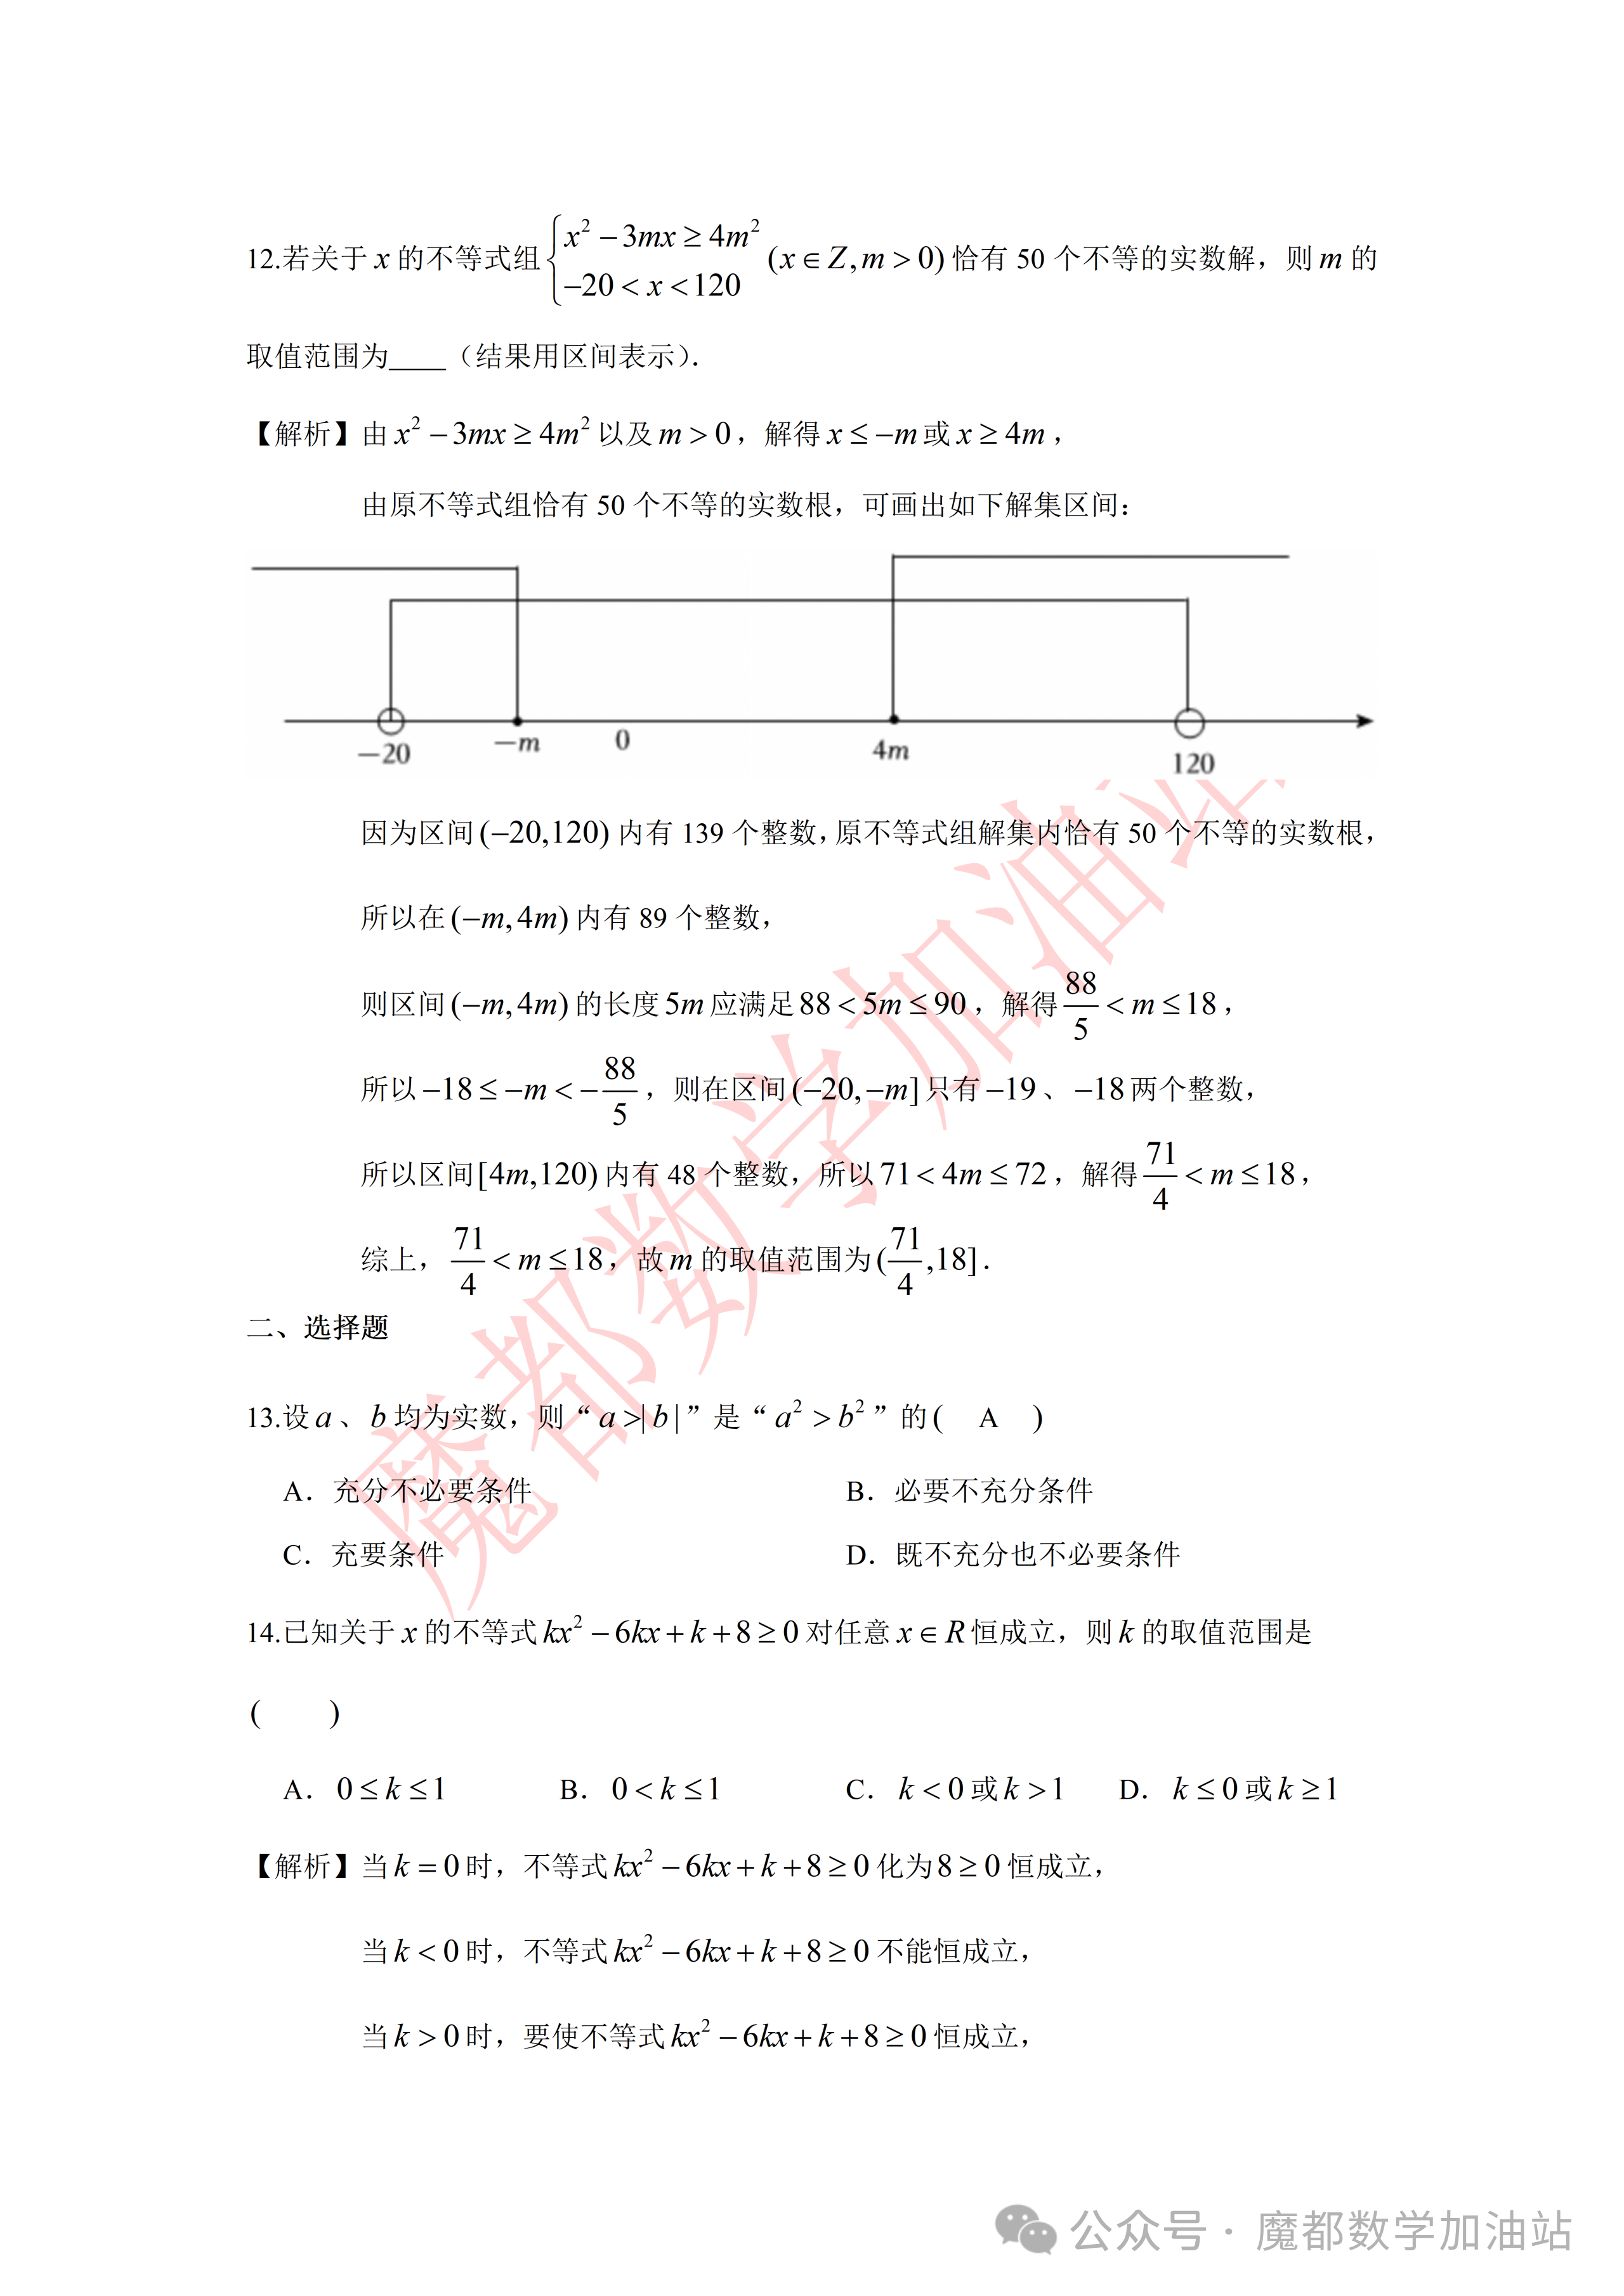
\includegraphics[width=.88\linewidth,trim=400bp 2410bp 320bp 860bp,clip]{../原图/高一46_交附闵行_国庆作业3/04.png}
\end{center}
\step{因为区间 $(-20,120)$ 内有 $139$ 个整数，原不等式组解集内有 $50$ 个不等的整数根，}
\step{所以在区间 $(-m,4m)$ 内有 $89$ 个整数，}
\step{则区间 $(-m,4m)$ 的长度 $5m$ 应满足 $88<5m\leqslant90$，解得 $\dfrac{88}{5}<m\leqslant18$，}
% 注：原卷题干称“实数解”，本行及后文按原卷解析照录为整数根计数。
\step{所以 $-18\leqslant-m<-\dfrac{88}{5}$，则在区间 $(-20,-m]$ 内有 $-19$、$-18$ 两个整数，}
\step{所以区间 $[4m,120)$ 内有 $48$ 个整数，}
\step{则 $71<4m\leqslant72$，解得 $\dfrac{71}{4}<m\leqslant18$，}
\step{综上，$\dfrac{71}{4}<m\leqslant18$，故 $m$ 的取值范围为 $\left(\dfrac{71}{4},18\right]$.}
\solend
\fi

\end{enumerate}

\bigsec{二、选择题}

\begin{enumerate}
\setcounter{enumi}{12}

\item 设 $a$、$b$ 均为实数，则“$a>|b|$”是“$a^2>b^2$”的\mbox{（\quad）}

\keepwithprev
A. 充分不必要条件\qquad B. 必要不充分条件

C. 充要条件\qquad\qquad D. 既不充分也不必要条件

\ans{$A$}

\item 已知关于 $x$ 的不等式 $kx^2-6kx+k+8\geqslant0$ 对任意 $x\in\R$ 恒成立，则 $k$ 的取值范围是\mbox{（\quad）}

\keepwithprev
A. $0\leqslant k\leqslant1$\qquad B. $0<k\leqslant1$

C. $k<0$ 或 $k>1$\qquad D. $k\leqslant0$ 或 $k\geqslant1$

\ans{$A$}

\ifanswer
\solbegin
\step{当 $k=0$ 时，不等式 $kx^2-6kx+k+8\geqslant0$ 化为 $8\geqslant0$ 恒成立，}
\step{当 $k<0$ 时，不等式 $kx^2-6kx+k+8\geqslant0$ 不能恒成立，}
\step{当 $k>0$ 时，要使不等式 $kx^2-6kx+k+8\geqslant0$ 恒成立，}
\step{需 $\Delta=36k^2-4(k^2+8k)\leqslant0$，解得 $0\leqslant k\leqslant1$，故选 $A$.}
\solend
\fi

\item 已知关于 $x$ 的不等式 $a\leqslant\dfrac34x^2-3x+4\leqslant b$，下列结论正确的是\mbox{（\quad）}

\keepwithprev
A. 当 $a<b<1$ 时，不等式 $a\leqslant\dfrac34x^2-3x+4\leqslant b$ 的解集非空

B. 当 $a=2$ 时，不等式 $a\leqslant\dfrac34x^2-3x+4\leqslant b$ 的解集可以为 $\{x\mid c\leqslant x\leqslant d\}$ 的形式

C. 不等式 $a\leqslant\dfrac34x^2-3x+4\leqslant b$ 的解集恰好为 $\{x\mid a\leqslant x\leqslant b\}$，那么 $b=\dfrac43$

D. 不等式 $a\leqslant\dfrac34x^2-3x+4\leqslant b$ 的解集恰好为 $\{x\mid a\leqslant x\leqslant b\}$，那么 $b-a=4$

\ans{$D$}

\ifanswer
\solbegin
\step{由 $\dfrac34x^2-3x+4\leqslant b$，得 $3x^2-12x+16-4b\leqslant0$，又 $b<1$，}
\step{所以 $\Delta=144-12(16-4b)=48(b-1)<0$，从而不等式无解，故 $A$ 错误；}
\step{在同一平面直角坐标系中作出函数 $y=\dfrac34x^2-3x+4=\dfrac34(x-2)^2+1$ 的图象及直线 $y=a$ 和 $y=b$，如图所示.}
\begin{center}
% 原图第 5 页解析配图直接裁取。
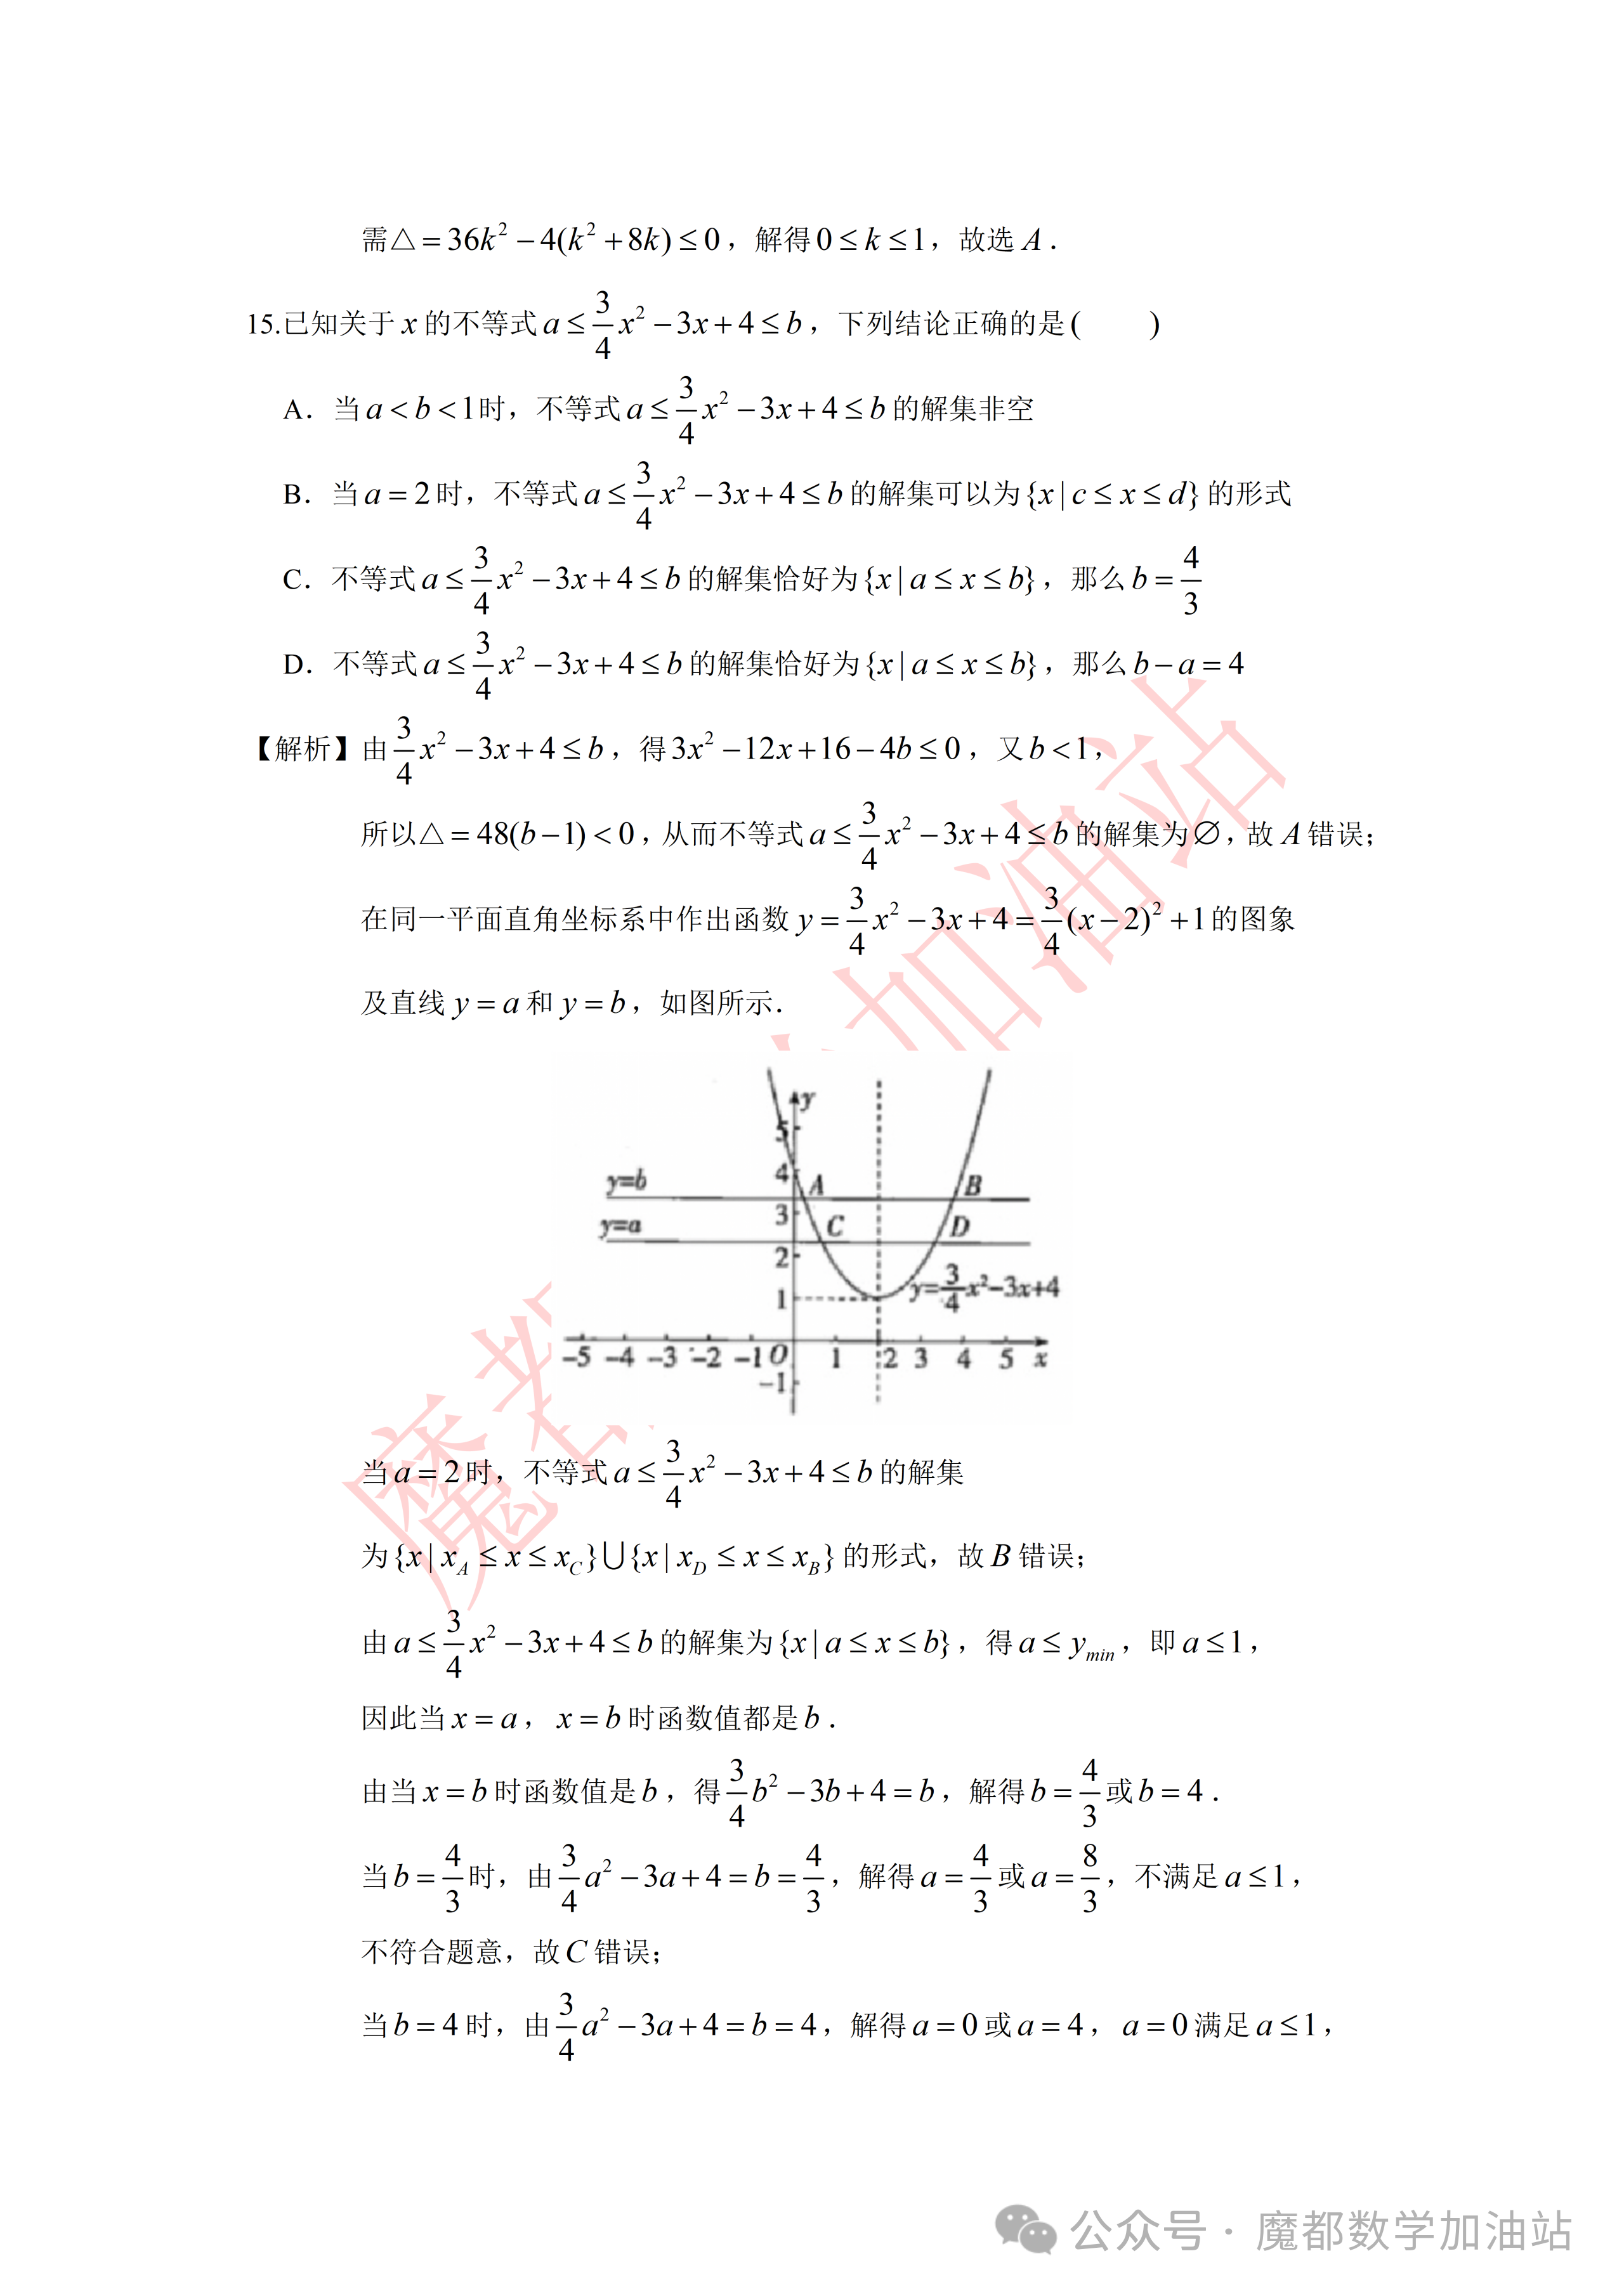
\includegraphics[width=.55\linewidth,trim=900bp 1400bp 760bp 1680bp,clip]{../原图/高一46_交附闵行_国庆作业3/05.png}
\end{center}
\step{当 $a=2$ 时，不等式 $a\leqslant\dfrac34x^2-3x+4\leqslant b$ 的解集为
$\{x\mid x_A\leqslant x\leqslant x_C\}\cup\{x\mid x_D\leqslant x\leqslant x_B\}$ 的形式，故 $B$ 错误；}
\step{由 $a\leqslant\dfrac34x^2-3x+4\leqslant b$ 的解集恰好为 $\{x\mid a\leqslant x\leqslant b\}$ 的形式，得 $a\leqslant y_{\min}$，即 $a\leqslant1$，}
\step{因为当 $x=a$、$x=b$ 时函数值都是 $b$，当 $x=a$ 时，$\dfrac34a^2-3a+4=b$；当 $x=b$ 时，$\dfrac34b^2-3b+4=b$，}
\step{解得 $b=\dfrac43$ 或 $b=4$，}
\step{当 $b=\dfrac43$ 时，由 $\dfrac34a^2-3a+4=b$，解得 $a=\dfrac43$ 或 $a=\dfrac83$，不符合题意，故 $C$ 错误；}
\step{当 $b=4$ 时，由 $\dfrac34a^2-3a+4=b$，解得 $a=0$ 或 $a=4$，$a=0$ 满足 $a\leqslant1$，故 $D$ 正确；}
\step{故选 $D$.}
\solend
\fi

\item 已知 $x$、$y\in(0,+\infty)$，则 $(x-y)^2+2y+1-x+\dfrac4x$ 的最小值为\mbox{（\quad）}

\keepwithprev
A. $1$\qquad B. $2$\qquad C. $3$\qquad D. $4$

\ans{$D$}

\ifanswer
\solbegin
\step{因为 $(x-y)^2+2y+1-x+\dfrac4x=(x-y-1)^2+x+\dfrac4x$，}
\step{当且仅当 $x-y-1=0$，且 $x=\dfrac4x$ 时取等号，}
\step{又因为 $x+\dfrac4x\geqslant2\sqrt{x\cdot\dfrac4x}=4$，当且仅当 $x=2$ 时取等号，}
\step{故选 $D$.}
\solend
\fi

\end{enumerate}

\bigsec{三、解答题}

\begin{enumerate}
\setcounter{enumi}{16}

\item 设集合 $A=\left\{x\middle|\dfrac{x-3}{x-1}<0\right\}$，$B=\{x\mid x^2-2ax+a^2-1>0\}$.
\begin{enumerate}[label=(\arabic*)]
\item 若 $a=3$，求 $A\cup B$；
\item 若“$x\in A$”是“$x\in B$”的充分条件，求实数 $a$ 的取值范围.
\end{enumerate}

\ifanswer
\solbegin
% 注：原卷题干为 a^2-1，故 a=3 时常数项为 8；题干与本步一致。
\stepm{(1)}{当 $a=3$ 时，$B=\{x\mid x^2-6x+8>0\}=\{x\mid x<2\text{ 或 }x>4\}$；}
\step{因为 $A=\left\{x\middle|\dfrac{x-3}{x-1}<0\right\}=\{x\mid(x-1)(x-3)<0\}=\{x\mid1<x<3\}$，}
\step{所以 $A\cup B=\{x\mid x<2\text{ 或 }x>4\}\cup\{x\mid1<x<3\}
=\{x\mid x<3\text{ 或 }x>4\}$.}
\stepm{(2)}{因为“$x\in A$”是“$x\in B$”的充分条件，所以 $A\subseteq B$，}
\step{因 $A=\left\{x\middle|\dfrac{x-3}{x-1}<0\right\}
=\{x\mid(x-1)(x-3)<0\}=\{x\mid1<x<3\}$，}
\step{所以 $A\subseteq B=\{x\mid x<a-1\text{ 或 }x>a+1\}$，}
\step{要使 $A\subseteq B$，需有 $a-1\geqslant3$ 或 $a+1\leqslant1$，}
\step{所以 $a\geqslant4$ 或 $a\leqslant0$，故 $a$ 的取值范围为 $\{a\mid a\geqslant4\text{ 或 }a\leqslant0\}$.}
\solend
\fi

\ansspace[6]

\item 某学校引入种植类劳动教育课程，打算围成如图所示的四块全等的长方形田地种植不同种类的蔬菜，其中一面可以利用原有的墙（足够长），其他各面需要用篱笆围成，设其中一块田地为矩形 $ABCD$.

\begin{center}
% 原图第 6 页配图直接裁取。
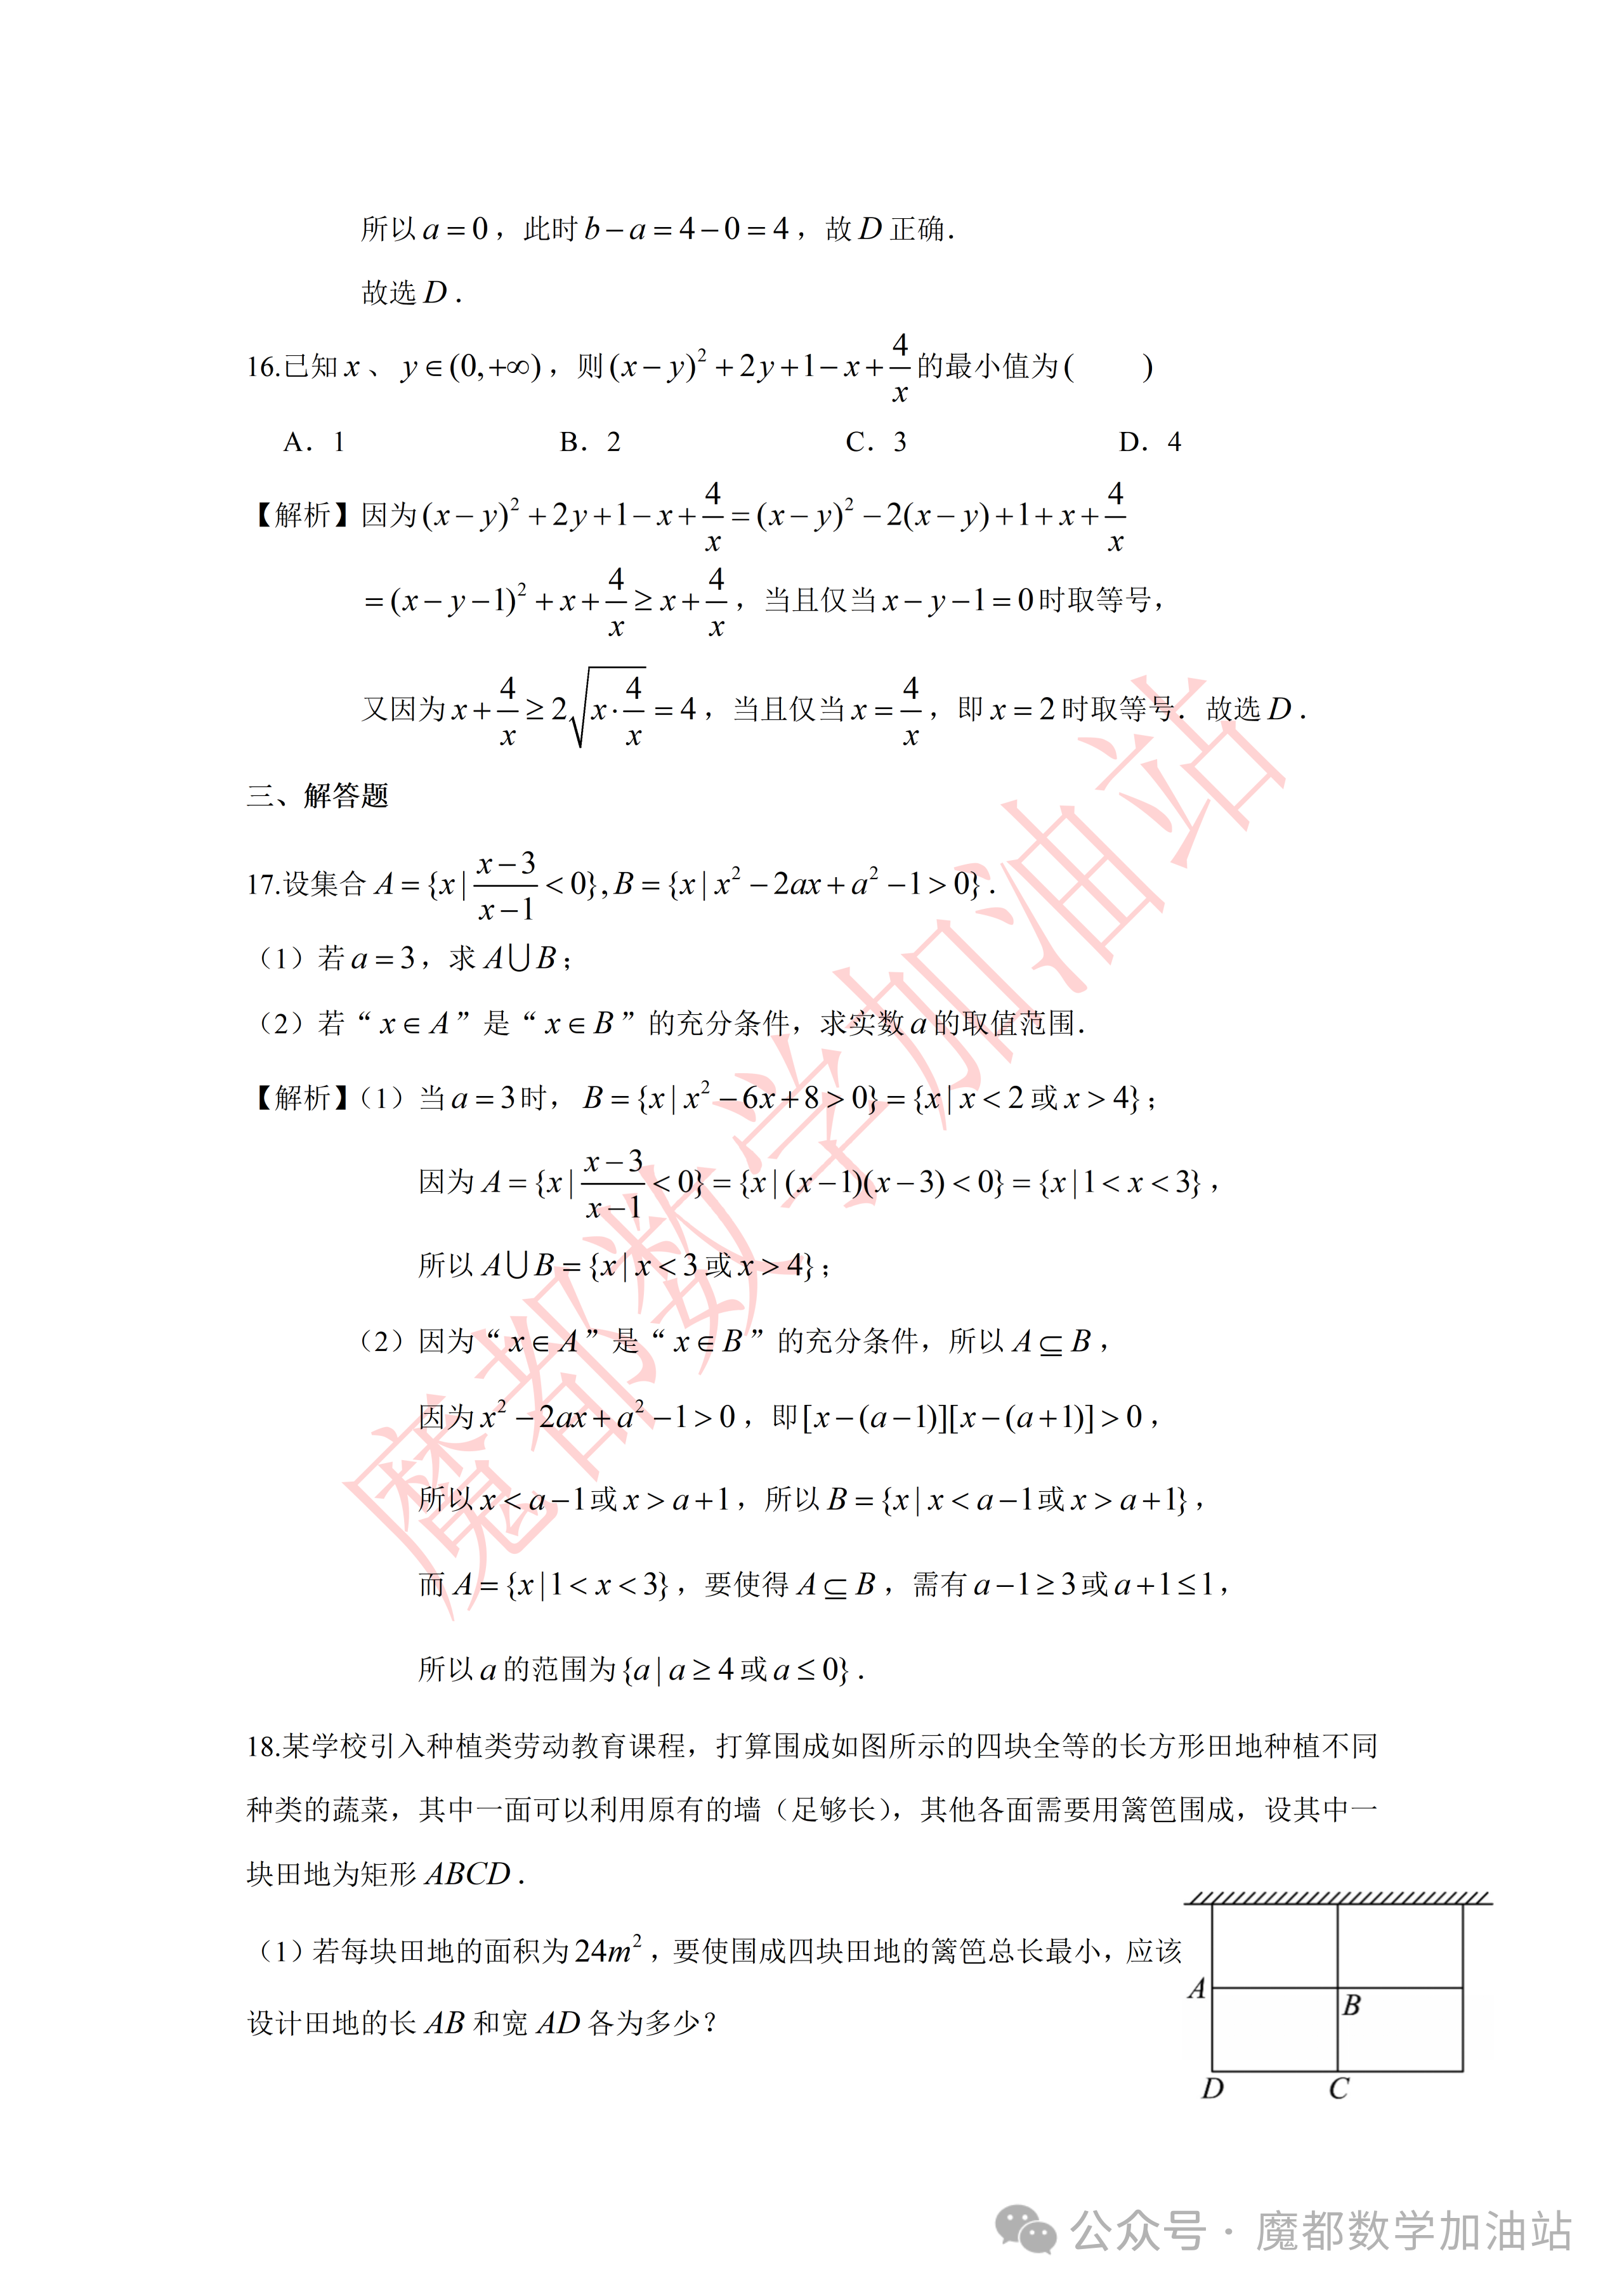
\includegraphics[width=.33\linewidth,trim=1866bp 220bp 210bp 2960bp,clip]{../原图/高一46_交附闵行_国庆作业3/06.png}
\end{center}

\begin{enumerate}[label=(\arabic*)]
\item 若每块田地的面积为 $24\,\text{m}^2$，要使围成四块田地的篱笆总长最小，应该设计田地的长 $AB$ 和宽 $AD$ 各为多少？
\item 现有 $40\,\text{m}$ 长的篱笆，要使每块田地的面积最大，应该设计田地的长 $AB$ 和宽 $AD$ 各为多少？
\end{enumerate}

\ifanswer
\solbegin
\stepm{(1)}{设 $AB$ 长为 $x\,\text{m}$，$AD$ 宽为 $y\,\text{m}$，由题意得 $xy=24$，篱笆总长为 $4x+6y$，}
\step{$4x+6y\geqslant2\sqrt{4x\cdot6y}=2\sqrt{24xy}=48$，}
\step{当且仅当 $4x=6y$ 时取等号，解得 $x=6$，$y=4$，}
\step{所以田地的长 $AB$ 为 $6\,\text{m}$，宽 $AD$ 为 $4\,\text{m}$.}
\stepm{(2)}{设 $AB$ 长为 $a\,\text{m}$，$AD$ 宽为 $b\,\text{m}$，由篱笆总长 $4a+6b=40$，即 $2a+3b=20$，}
\step{将 $a=\dfrac{20-3b}{2}$ 代入每块田地面积 $ab$，得 $ab=\dfrac12b(20-3b)=-\dfrac32b^2+10b$，}
\step{当 $b=\dfrac{10}{3}$ 时，$ab$ 最大，此时 $a=5$，}
\step{所以田地的长 $AB$ 为 $5\,\text{m}$，宽 $AD$ 为 $\dfrac{10}{3}\,\text{m}$.}
\solend
\fi

\ansspace[8]

\item 已知 $x_1$、$x_2$ 是一元二次方程 $4kx^2-4kx+k+1=0$ 的两个不等实数根.
\begin{enumerate}[label=(\arabic*)]
\item 若 $x_1$、$x_2$ 均为正根，求实数 $k$ 的取值范围；
\item 求使 $\dfrac{x_1}{x_2}+\dfrac{x_2}{x_1}-2$ 的值为整数 $k$ 的整数值.
\end{enumerate}

\ifanswer
\solbegin
\stepm{(1)}{由题意，$x_1$、$x_2$ 是方程 $4kx^2-4kx+k+1=0$ 的两个不等实数根，}
\step{故 $k\neq0$，$\Delta=(-4k)^2-16k(k+1)>0$，得 $-16k>0$，所以 $k<0$，}
\step{又 $x_1+x_2=1$，$x_1x_2=\dfrac{k+1}{4k}>0$，得 $k+1<0$，}
\step{所以 $k$ 的取值范围为 $(-\infty,-1)$.}
\stepm{(2)}{由题意，}
\step{$\dfrac{x_1}{x_2}+\dfrac{x_2}{x_1}-2
=\dfrac{x_1^2+x_2^2-2x_1x_2}{x_1x_2}
=\dfrac{(x_1+x_2)^2-4x_1x_2}{x_1x_2}$，}
\step{又 $x_1+x_2=1$，$x_1x_2=\dfrac{k+1}{4k}$，}
\step{则 $\dfrac{x_1}{x_2}+\dfrac{x_2}{x_1}-2=-\dfrac4{k+1}$，}
\step{由于 $-\dfrac4{k+1}$ 为整数，故 $k+1$ 只能取 $\pm1$、$\pm2$、$\pm4$，又 $k<-1$，}
\step{所以整数 $k$ 的值为 $-2$、$-3$、$-5$.}
\solend
\fi

\ansspace[8]

\item 已知 $a>0$，$b>0$，且 $2a+3b=3$.
\begin{enumerate}[label=(\arabic*)]
\item 求 $ab$ 的最大值；
\item 求 $a-\dfrac1{6b}$ 的最大值；
\item 求 $\dfrac2a+\dfrac3{b+1}$ 的最小值.
\end{enumerate}

\ifanswer
\solbegin
\stepm{(1)}{由 $2a+3b=3$，得 $3=2a+3b\geqslant2\sqrt{6ab}$，}
\step{所以 $ab\leqslant\dfrac38$，当且仅当 $2a=3b=\dfrac32$ 时取等号，}
\step{故 $ab$ 的最大值为 $\dfrac38$.}
\stepm{(2)}{由 $2a+3b=3$，得 $a=\dfrac32-\dfrac32b$，}
\step{则 $a-\dfrac1{6b}=\dfrac32-\dfrac32b-\dfrac1{6b}$，}
\step{由基本不等式，$\dfrac32b+\dfrac1{6b}\geqslant2\sqrt{\dfrac32b\cdot\dfrac1{6b}}=1$，}
\step{当且仅当 $\dfrac32b=\dfrac1{6b}$，即 $b=\dfrac13$、$a=1$ 时取等号，}
\step{所以 $a-\dfrac1{6b}$ 的最大值为 $\dfrac12$.}
\stepm{(3)}{由 $2a+3b=3$，得 $2a+3(b+1)=6$，}
\step{$\dfrac2a+\dfrac3{b+1}
=\dfrac16\left(2a+3(b+1)\right)\left(\dfrac2a+\dfrac3{b+1}\right)$}
\step{$=\dfrac16\left(13+\dfrac{6(b+1)}a+\dfrac{6a}{b+1}\right)
\geqslant\dfrac16\left(13+2\sqrt{\dfrac{6(b+1)}a\cdot\dfrac{6a}{b+1}}\right)=\dfrac{25}{6}$，}
\step{当且仅当 $a=b+1$，即 $a=\dfrac65$、$b=\dfrac15$ 时取等号，}
\step{所以 $\dfrac2a+\dfrac3{b+1}$ 的最小值为 $\dfrac{25}{6}$.}
\solend
\fi

\ansspace[8]

\item 已知 $U=\R$ 为全集，集合 $A=\{s^2+3t^2\mid s,t\in U\}$.
\begin{enumerate}[label=(\arabic*)]
\item 设 $U=\{1,3,5\}$，求集合 $A$ 的元素个数；
\item 设 $U=\Z$，证明：若 $x\in A$，则 $7x\in A$；
\item 设 $U=\R$，$x$、$y\in A$，且 $x=m^2+3n^2$，$y=p^2+3q^2$，若 $mp-3nq=\sqrt3$，求 $x+y+mq+np$ 的最小值.
\end{enumerate}

\ifanswer
\solbegin
\stepm{(1)}{当 $s=1$，$t=1$ 时，$s^2+3t^2=1+3=4$；}
\step{当 $s=1$，$t=3$ 时，$s^2+3t^2=1+27=28$；}
\step{当 $s=1$，$t=5$ 时，$s^2+3t^2=1+75=76$；}
\step{当 $s=3$，$t=1$ 时，$s^2+3t^2=9+3=12$；}
\step{当 $s=3$，$t=3$ 时，$s^2+3t^2=9+27=36$；}
\step{当 $s=3$，$t=5$ 时，$s^2+3t^2=9+75=84$；}
\step{当 $s=5$，$t=1$ 时，$s^2+3t^2=25+3=28$；}
\step{当 $s=5$，$t=3$ 时，$s^2+3t^2=25+27=52$；}
\step{当 $s=5$，$t=5$ 时，$s^2+3t^2=25+75=100$，}
\step{所以 $A=\{4,12,28,36,52,76,84,100\}$，有 $8$ 个元素.}
\stepm{(2)}{因为 $U=\Z$，$x\in A$，设 $x=s^2+3t^2$，}
\step{则 $7x=7(s^2+3t^2)=(2s+3t)^2+3(s-2t)^2\in A$，}
\step{所以 $7x\in A$.}
\stepm{(3)}{因为 $x=m^2+3n^2$，$y=p^2+3q^2$，}
\step{$xy=(m^2+3n^2)(p^2+3q^2)=3(mq+np)^2+(mp-3nq)^2$，}
\step{设 $mq+np=b$，则 $xy=3b^2+3$，所以 $y=\dfrac{3b^2+3}{x}$，}
\step{于是 $x+y+mq+np=x+\dfrac{3b^2+3}{x}+b\geqslant2\sqrt{3b^2+3}+b$，}
\step{设 $2\sqrt{3b^2+3}+b=t$，整理得 $11b^2+2bt+12-t^2=0$，}
\step{判别式法，$\Delta=4t^2-44(12-t^2)\geqslant0$，得 $t\geqslant\sqrt{11}$，}
\step{即 $(x+y+mq+np)_{\min}=\sqrt{11}$，所以 $x+y+mq+np$ 的最小值为 $\sqrt{11}$.}
\solend
\fi

\ansspace*[10]

\end{enumerate}

\end{document}
"
% 紧凑版：xelatex "\def\iscompact{1}% 高一46_交附闵行_国庆作业3.tex
%   —— 高一上数学“2026-2027 年交附闵行高一上国庆作业 3”（讲评版）
% 试卷版：xelatex 高一46_交附闵行_国庆作业3.tex
% 答案版：xelatex "\def\isanswer{1}% 高一46_交附闵行_国庆作业3.tex
%   —— 高一上数学“2026-2027 年交附闵行高一上国庆作业 3”（讲评版）
% 试卷版：xelatex 高一46_交附闵行_国庆作业3.tex
% 答案版：xelatex "\def\isanswer{1}% 高一46_交附闵行_国庆作业3.tex
%   —— 高一上数学“2026-2027 年交附闵行高一上国庆作业 3”（讲评版）
% 试卷版：xelatex 高一46_交附闵行_国庆作业3.tex
% 答案版：xelatex "\def\isanswer{1}\input{高一46_交附闵行_国庆作业3.tex}"
% 紧凑版：xelatex "\def\iscompact{1}\input{高一46_交附闵行_国庆作业3.tex}"
%
% 原始材料：微信公众号“魔都数学加油站”，作者破晓，2026-10-02 17:56 发布。
% 原文标题：“27学年高一46——2026-2027你那上海市交附闵行高一上国庆作业3”
% （公众号标题中的“你那”照录，系原文标题字样）；原文链接：
% http://mp.weixin.qq.com/s?__biz=Mzg4ODU1ODMxOQ==&mid=2247591657&idx=3&sn=a894d1a16611283a61b3eaba32a3f24c&chksm=cee83366c6a55381b370069f84ef63d20251f94608bb37cc4ec2d66227401bd147f4f6bd8256&scene=126&sessionid=1790935402&subscene=7&clicktime=1790937618&enterid=1790937618#rd
% 正文为 9 张 PNG 页，按页序读取原图；第 01、02、07 页 4762×6735，
% 第 03—06、08、09 页 2560×3620。卷面标题照原卷印作“2026-2027 年交附闵行高一上国庆作业 3”。
% 原文从第 3 题起，题号照原卷保留；正文为讲评版，答案、解析依原卷顺序录入。
% 水印及页脚公众号标识不录入。卷面插图直接裁取对应原图页，不另制图片文件。
%
% 与原卷的排版差异：
%   ① 原卷按“一、填空题”“二、选择题”“三、解答题”分节，本稿沿用原节与原题号，
%      只改排为全稿统一的大节样式；
%   ② 原卷答案与解析依页面位置分布，本稿按 common.sty 统一置于答案版；
%   ③ 原卷副标题未印，本稿按“知识模块”口径标作“集合与常用逻辑用语、不等式”。
%
% 原卷存疑一处（照抄未改，见第 12 题题干及解析处注释）：
%   第 12 题题干同时给出 x∈Z，却称不等式组有“50 个不等的实数解”；解析按整数根计数。
%   此处题干与解析的原文不一致，本稿均照录。
% 第 17 题曾疑似有常数项不一致：复核原图题干为 a^2-1，a=3 时常数项确为 8，
% 与解析相符；不将其记作原卷错误。
%
\documentclass[a4paper,11pt]{article}
\usepackage{common}

\begin{document}

\examtitlest[3]{2026--2027 年交附闵行高一上国庆作业 3}{集合与常用逻辑用语、不等式}

\bigsec{一、填空题}

\begin{enumerate}
\setcounter{enumi}{2}

\item 不等式 $\dfrac{x^2-10}{x+2}\geqslant1$ 的解集为\blankline[4.4em].

\ifanswer
\ans{$\{x\mid-3\leqslant x<-2\text{ 或 }x\geqslant4\}$}
\solbegin
\step{不等式 $\dfrac{x^2-10}{x+2}\geqslant1$，移项得 $\dfrac{x^2-10}{x+2}-1\geqslant0$，}
\step{通分得 $\dfrac{x^2-x-12}{x+2}\geqslant0$，即 $\dfrac{(x-4)(x+3)}{x+2}\geqslant0$，}
\step{解得 $-3\leqslant x<-2$ 或 $x\geqslant4$，}
\step{故不等式的解集为 $\{x\mid-3\leqslant x<-2\text{ 或 }x\geqslant4\}$.}
\solend
\fi

\item $|x-3|+|x-5|\geqslant2$，当等号成立时，$x$ 的范围是\blankline[4.4em].

\ifanswer
\ans{$[3,5]$}
\fi

\item 若直角三角形斜边长等于 $4\sqrt2\,\text{cm}$，则直角三角形面积的最大值为\blankline[4.4em].

\ifanswer
\solbegin
\step{设 $Rt\triangle ABC$ 中，$C=90^\circ$，则 $c=\sqrt{a^2+b^2}=4\sqrt2$，所以 $a^2+b^2=32$，}
\step{由基本不等式得 $a^2+b^2\geqslant2ab$，当且仅当 $a=b=4$ 时取等号，}
\step{所以 $\triangle ABC$ 的面积 $S=\dfrac12ab\leqslant8$，}
\step{当且仅当 $a=b=4$ 时，$\triangle ABC$ 的面积最大值为 $8$.}
\solend
\fi

\item 不等式 $(x-1)(2-x)>0$ 的解集为\blankline[4.4em].

\ifanswer
\solbegin
\step{$(x-1)(2-x)>0\Rightarrow(x-1)(x-2)<0$，}
\step{故不等式的解集为 $\{x\mid1<x<2\}$.}
\solend
\fi

\item 已知集合 $A=\{1,2\}$，$B=\{x\mid x^2-2mx+m=0\}$，$A\cup B=A$，则实数 $m$ 的取值范围为\blankline[4.4em].

\ifanswer
\solbegin
\step{因为 $A\cup B=A$，所以 $B\subseteq A$，}
\step{当 $B=\varnothing$ 时，$\Delta=(-2m)^2-4m<0$，解得 $0<m<1$，}
\step{当 $B$ 为单元素集时，$\Delta=0$，解得 $m=0$ 或 $m=1$，}
\step{当 $m=0$ 时，方程 $x^2=0$，解得 $x=0$，此时 $B=\{0\}$，不满足 $B\subseteq A$；}
\step{当 $m=1$ 时，方程 $x^2-2x+1=0$，解得 $x=1$，此时 $B=\{1\}$，满足 $B\subseteq A$；}
\step{当 $B=\{1,2\}$ 时，由韦达定理得 $1+2=2m$，$1\times2=m$，无解，}
\step{综上所述，实数 $m$ 的取值范围为 $\{m\mid0<m\leqslant1\}$.}
\solend
\fi

\item 设 $a$、$b$、$c\in\R^+$，若 $a+b+c=1$，则 $\dfrac1a+\dfrac1b+\dfrac1c\geqslant$\blankline[4.4em].

\ifanswer
\solbegin
\step{因为 $a$、$b$、$c\in\R^+$，且 $a+b+c=1$，}
\step{所以 $\dfrac1a+\dfrac1b+\dfrac1c=(a+b+c)\left(\dfrac1a+\dfrac1b+\dfrac1c\right)$}
\step{$=3+\dfrac ab+\dfrac ba+\dfrac ac+\dfrac ca+\dfrac bc+\dfrac cb$，}
\step{由基本不等式得 $\dfrac ab+\dfrac ba\geqslant2$，$\dfrac ac+\dfrac ca\geqslant2$，$\dfrac bc+\dfrac cb\geqslant2$，}
\step{所以 $\dfrac1a+\dfrac1b+\dfrac1c\geqslant9$，当且仅当 $a=b=c=\dfrac13$ 时取等号，}
\step{所以 $\dfrac1a+\dfrac1b+\dfrac1c$ 的最小值为 $9$.}
\solend
\fi

\item 已知 $-1\leqslant x+y\leqslant2$，$-2\leqslant x-y\leqslant1$，则 $x-2y$ 的范围为\blankline[4.4em].

\ifanswer
\solbegin
\step{设 $x-2y=m(x+y)+n(x-y)$，}
\step{则 $x-2y=(m+n)x+(m-n)y$，所以 $m+n=1$，$m-n=-2$，}
\step{解得 $m=-\dfrac12$，$n=\dfrac32$，}
\step{所以 $x-2y=-\dfrac12(x+y)+\dfrac32(x-y)$，}
\step{因为 $-1\leqslant x+y\leqslant2$，$-2\leqslant x-y\leqslant1$，}
\step{所以 $-4\leqslant x-2y\leqslant2$，即 $x-2y$ 的范围为 $[-4,2]$.}
\solend
\fi

\item 设集合 $A=\{1,2,m\}$，其中 $m$ 为实数，令 $B=\{a^2\mid a\in A\}$，$C=A\cup B$. 若 $C$ 中所有元素之和为 $6$，则 $C$ 中的所有元素之积为\blankline[4.4em].

\ifanswer
\solbegin
\step{因为 $A=\{1,2,m\}$，所以 $B=\{a^2\mid a\in A\}=\{1,4,m^2\}$，$m\neq1$，$m\neq2$，}
\step{又 $C=A\cup B$，所以 $1\in C$，$4\in C$，$m^2\in C$，}
\step{若 $m^2=1$，则 $m=-1$ 或 $m=1$（舍），当 $m=-1$ 时，$C=\{1,2,4,-1\}$，$C$ 中所有元素之和为 $6$，}
\step{此时 $C$ 中所有元素之积为 $-8$；}
\step{若 $m^2=2$，则 $m=-\sqrt2$ 或 $m=\sqrt2$，$C$ 中所有元素之和不符合题意；}
\step{若 $m^2=4$，则 $m=-2$ 或 $m=2$，此时 $C=\{1,2,4,-2\}$ 或 $C=\{1,2,4\}$，所有元素之和不符合题意；}
\step{若 $m^2\neq1$，$m^2\neq2$，$m^2\neq4$，则 $C=\{1,2,4,m,m^2\}$，}
\step{所以 $1+2+4+m+m^2=6$，即 $m^2+m+1=0$，无解，}
\step{综上所述，$C$ 中所有元素之积为 $-8$.}
\solend
\fi

\item 若对任意实数 $x>0$，$y>0$，不等式 $x+\sqrt{xy}\leqslant a(x+y)$ 恒成立，则实数 $a$ 的最小值为\blankline[4.4em].

\ifanswer
\solbegin
\step{由不等式 $x+\sqrt{xy}\leqslant a(x+y)$ 对任意实数 $x>0$，$y>0$ 恒成立，}
\step{得 $a\geqslant\dfrac{x+\sqrt{xy}}{x+y}$，}
\step{设 $\sqrt{\dfrac yx}=t>0$，则 $a\geqslant\dfrac{1+t}{1+t^2}$，}
\step{$\dfrac{1+t}{1+t^2}\leqslant\dfrac{\sqrt2+1}{2}$，当且仅当 $t=\sqrt2-1$ 时取等号，}
\step{所以实数 $a$ 的最小值为 $\dfrac{\sqrt2+1}{2}$.}
\solend
\fi

% 注：原卷题干给出 x∈Z，却写“实数解”；解析按整数解计数，题干与解析不一致，照录未改。
\item 若关于 $x$ 的不等式组
$\begin{cases}x^2-3mx\geqslant4m^2\\-20<x<120\end{cases}$（$x\in\Z,m>0$）恰有 $50$ 个不等的实数解，则 $m$ 的取值范围为\blankline[4.4em]（结果用区间表示）.

\ifanswer
\solbegin
\step{由 $x^2-3mx\geqslant4m^2$ 以及 $m>0$，解得 $x\leqslant-m$ 或 $x\geqslant4m$，}
\step{由原不等式组恰有 $50$ 个不等的实数解，可画出如下解集区间：}
\begin{center}
% 原图第 4 页数轴图直接裁取。
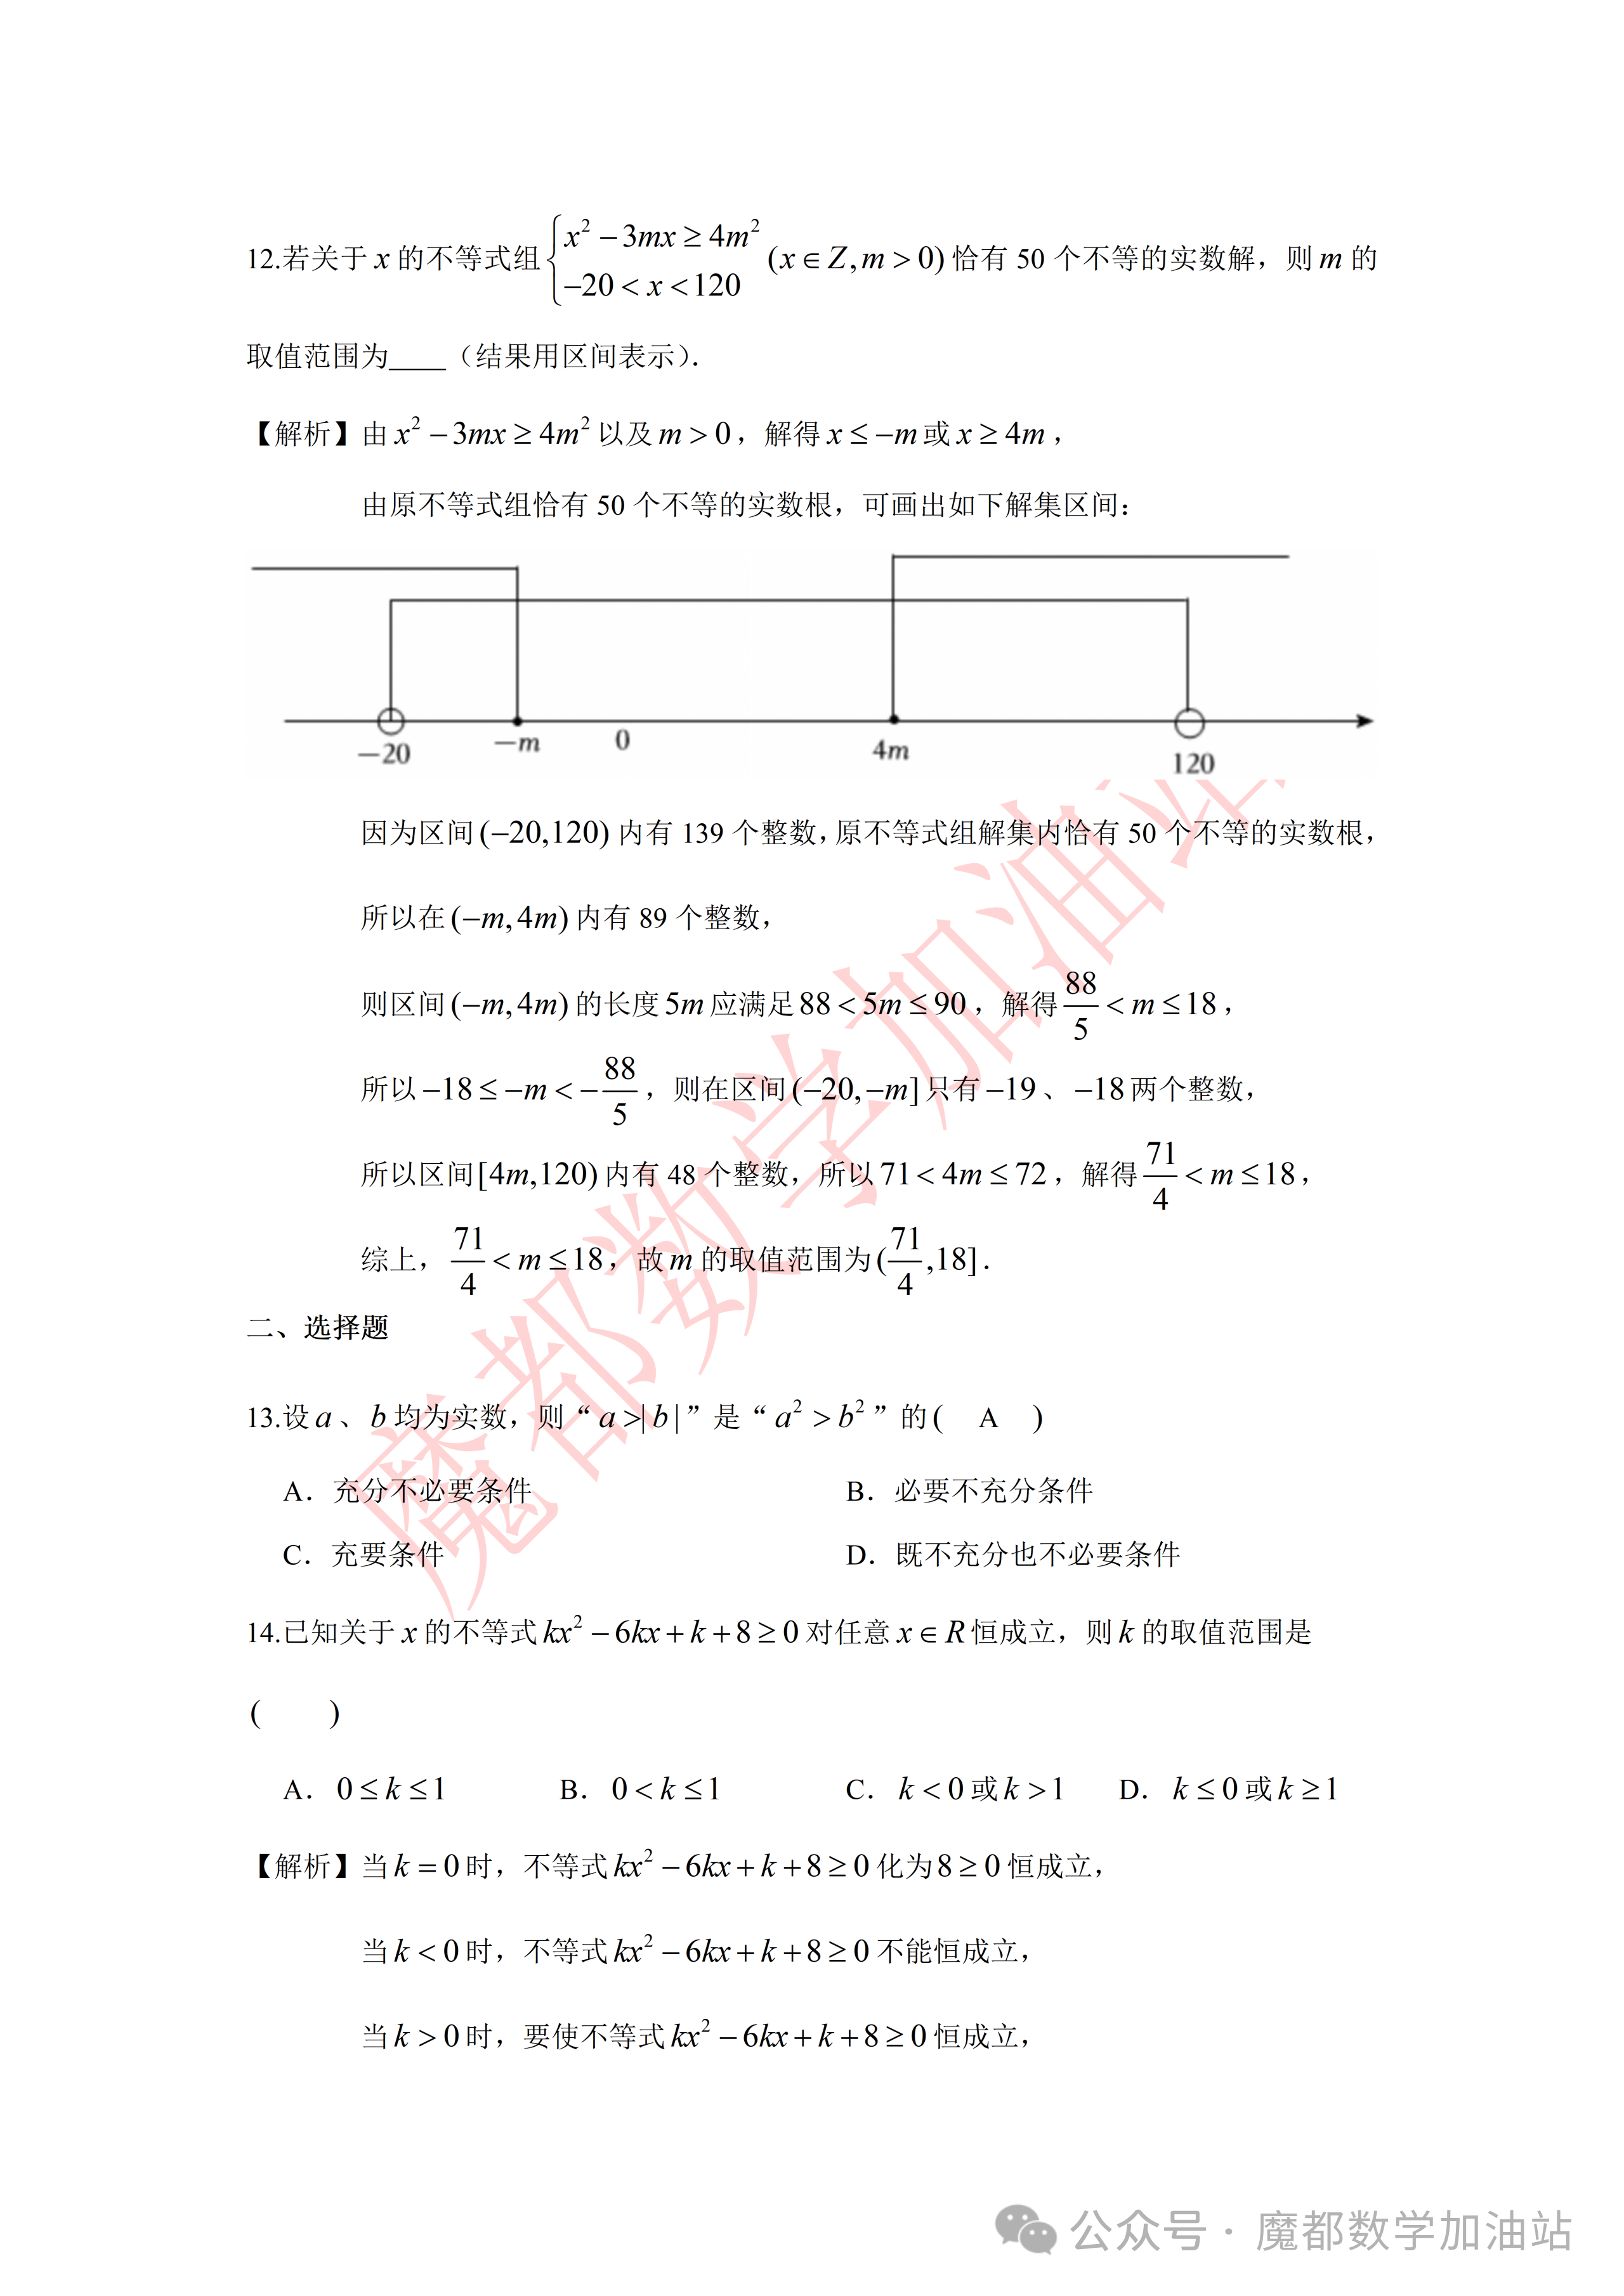
\includegraphics[width=.88\linewidth,trim=400bp 2410bp 320bp 860bp,clip]{../原图/高一46_交附闵行_国庆作业3/04.png}
\end{center}
\step{因为区间 $(-20,120)$ 内有 $139$ 个整数，原不等式组解集内有 $50$ 个不等的整数根，}
\step{所以在区间 $(-m,4m)$ 内有 $89$ 个整数，}
\step{则区间 $(-m,4m)$ 的长度 $5m$ 应满足 $88<5m\leqslant90$，解得 $\dfrac{88}{5}<m\leqslant18$，}
% 注：原卷题干称“实数解”，本行及后文按原卷解析照录为整数根计数。
\step{所以 $-18\leqslant-m<-\dfrac{88}{5}$，则在区间 $(-20,-m]$ 内有 $-19$、$-18$ 两个整数，}
\step{所以区间 $[4m,120)$ 内有 $48$ 个整数，}
\step{则 $71<4m\leqslant72$，解得 $\dfrac{71}{4}<m\leqslant18$，}
\step{综上，$\dfrac{71}{4}<m\leqslant18$，故 $m$ 的取值范围为 $\left(\dfrac{71}{4},18\right]$.}
\solend
\fi

\end{enumerate}

\bigsec{二、选择题}

\begin{enumerate}
\setcounter{enumi}{12}

\item 设 $a$、$b$ 均为实数，则“$a>|b|$”是“$a^2>b^2$”的\mbox{（\quad）}

\keepwithprev
A. 充分不必要条件\qquad B. 必要不充分条件

C. 充要条件\qquad\qquad D. 既不充分也不必要条件

\ans{$A$}

\item 已知关于 $x$ 的不等式 $kx^2-6kx+k+8\geqslant0$ 对任意 $x\in\R$ 恒成立，则 $k$ 的取值范围是\mbox{（\quad）}

\keepwithprev
A. $0\leqslant k\leqslant1$\qquad B. $0<k\leqslant1$

C. $k<0$ 或 $k>1$\qquad D. $k\leqslant0$ 或 $k\geqslant1$

\ans{$A$}

\ifanswer
\solbegin
\step{当 $k=0$ 时，不等式 $kx^2-6kx+k+8\geqslant0$ 化为 $8\geqslant0$ 恒成立，}
\step{当 $k<0$ 时，不等式 $kx^2-6kx+k+8\geqslant0$ 不能恒成立，}
\step{当 $k>0$ 时，要使不等式 $kx^2-6kx+k+8\geqslant0$ 恒成立，}
\step{需 $\Delta=36k^2-4(k^2+8k)\leqslant0$，解得 $0\leqslant k\leqslant1$，故选 $A$.}
\solend
\fi

\item 已知关于 $x$ 的不等式 $a\leqslant\dfrac34x^2-3x+4\leqslant b$，下列结论正确的是\mbox{（\quad）}

\keepwithprev
A. 当 $a<b<1$ 时，不等式 $a\leqslant\dfrac34x^2-3x+4\leqslant b$ 的解集非空

B. 当 $a=2$ 时，不等式 $a\leqslant\dfrac34x^2-3x+4\leqslant b$ 的解集可以为 $\{x\mid c\leqslant x\leqslant d\}$ 的形式

C. 不等式 $a\leqslant\dfrac34x^2-3x+4\leqslant b$ 的解集恰好为 $\{x\mid a\leqslant x\leqslant b\}$，那么 $b=\dfrac43$

D. 不等式 $a\leqslant\dfrac34x^2-3x+4\leqslant b$ 的解集恰好为 $\{x\mid a\leqslant x\leqslant b\}$，那么 $b-a=4$

\ans{$D$}

\ifanswer
\solbegin
\step{由 $\dfrac34x^2-3x+4\leqslant b$，得 $3x^2-12x+16-4b\leqslant0$，又 $b<1$，}
\step{所以 $\Delta=144-12(16-4b)=48(b-1)<0$，从而不等式无解，故 $A$ 错误；}
\step{在同一平面直角坐标系中作出函数 $y=\dfrac34x^2-3x+4=\dfrac34(x-2)^2+1$ 的图象及直线 $y=a$ 和 $y=b$，如图所示.}
\begin{center}
% 原图第 5 页解析配图直接裁取。
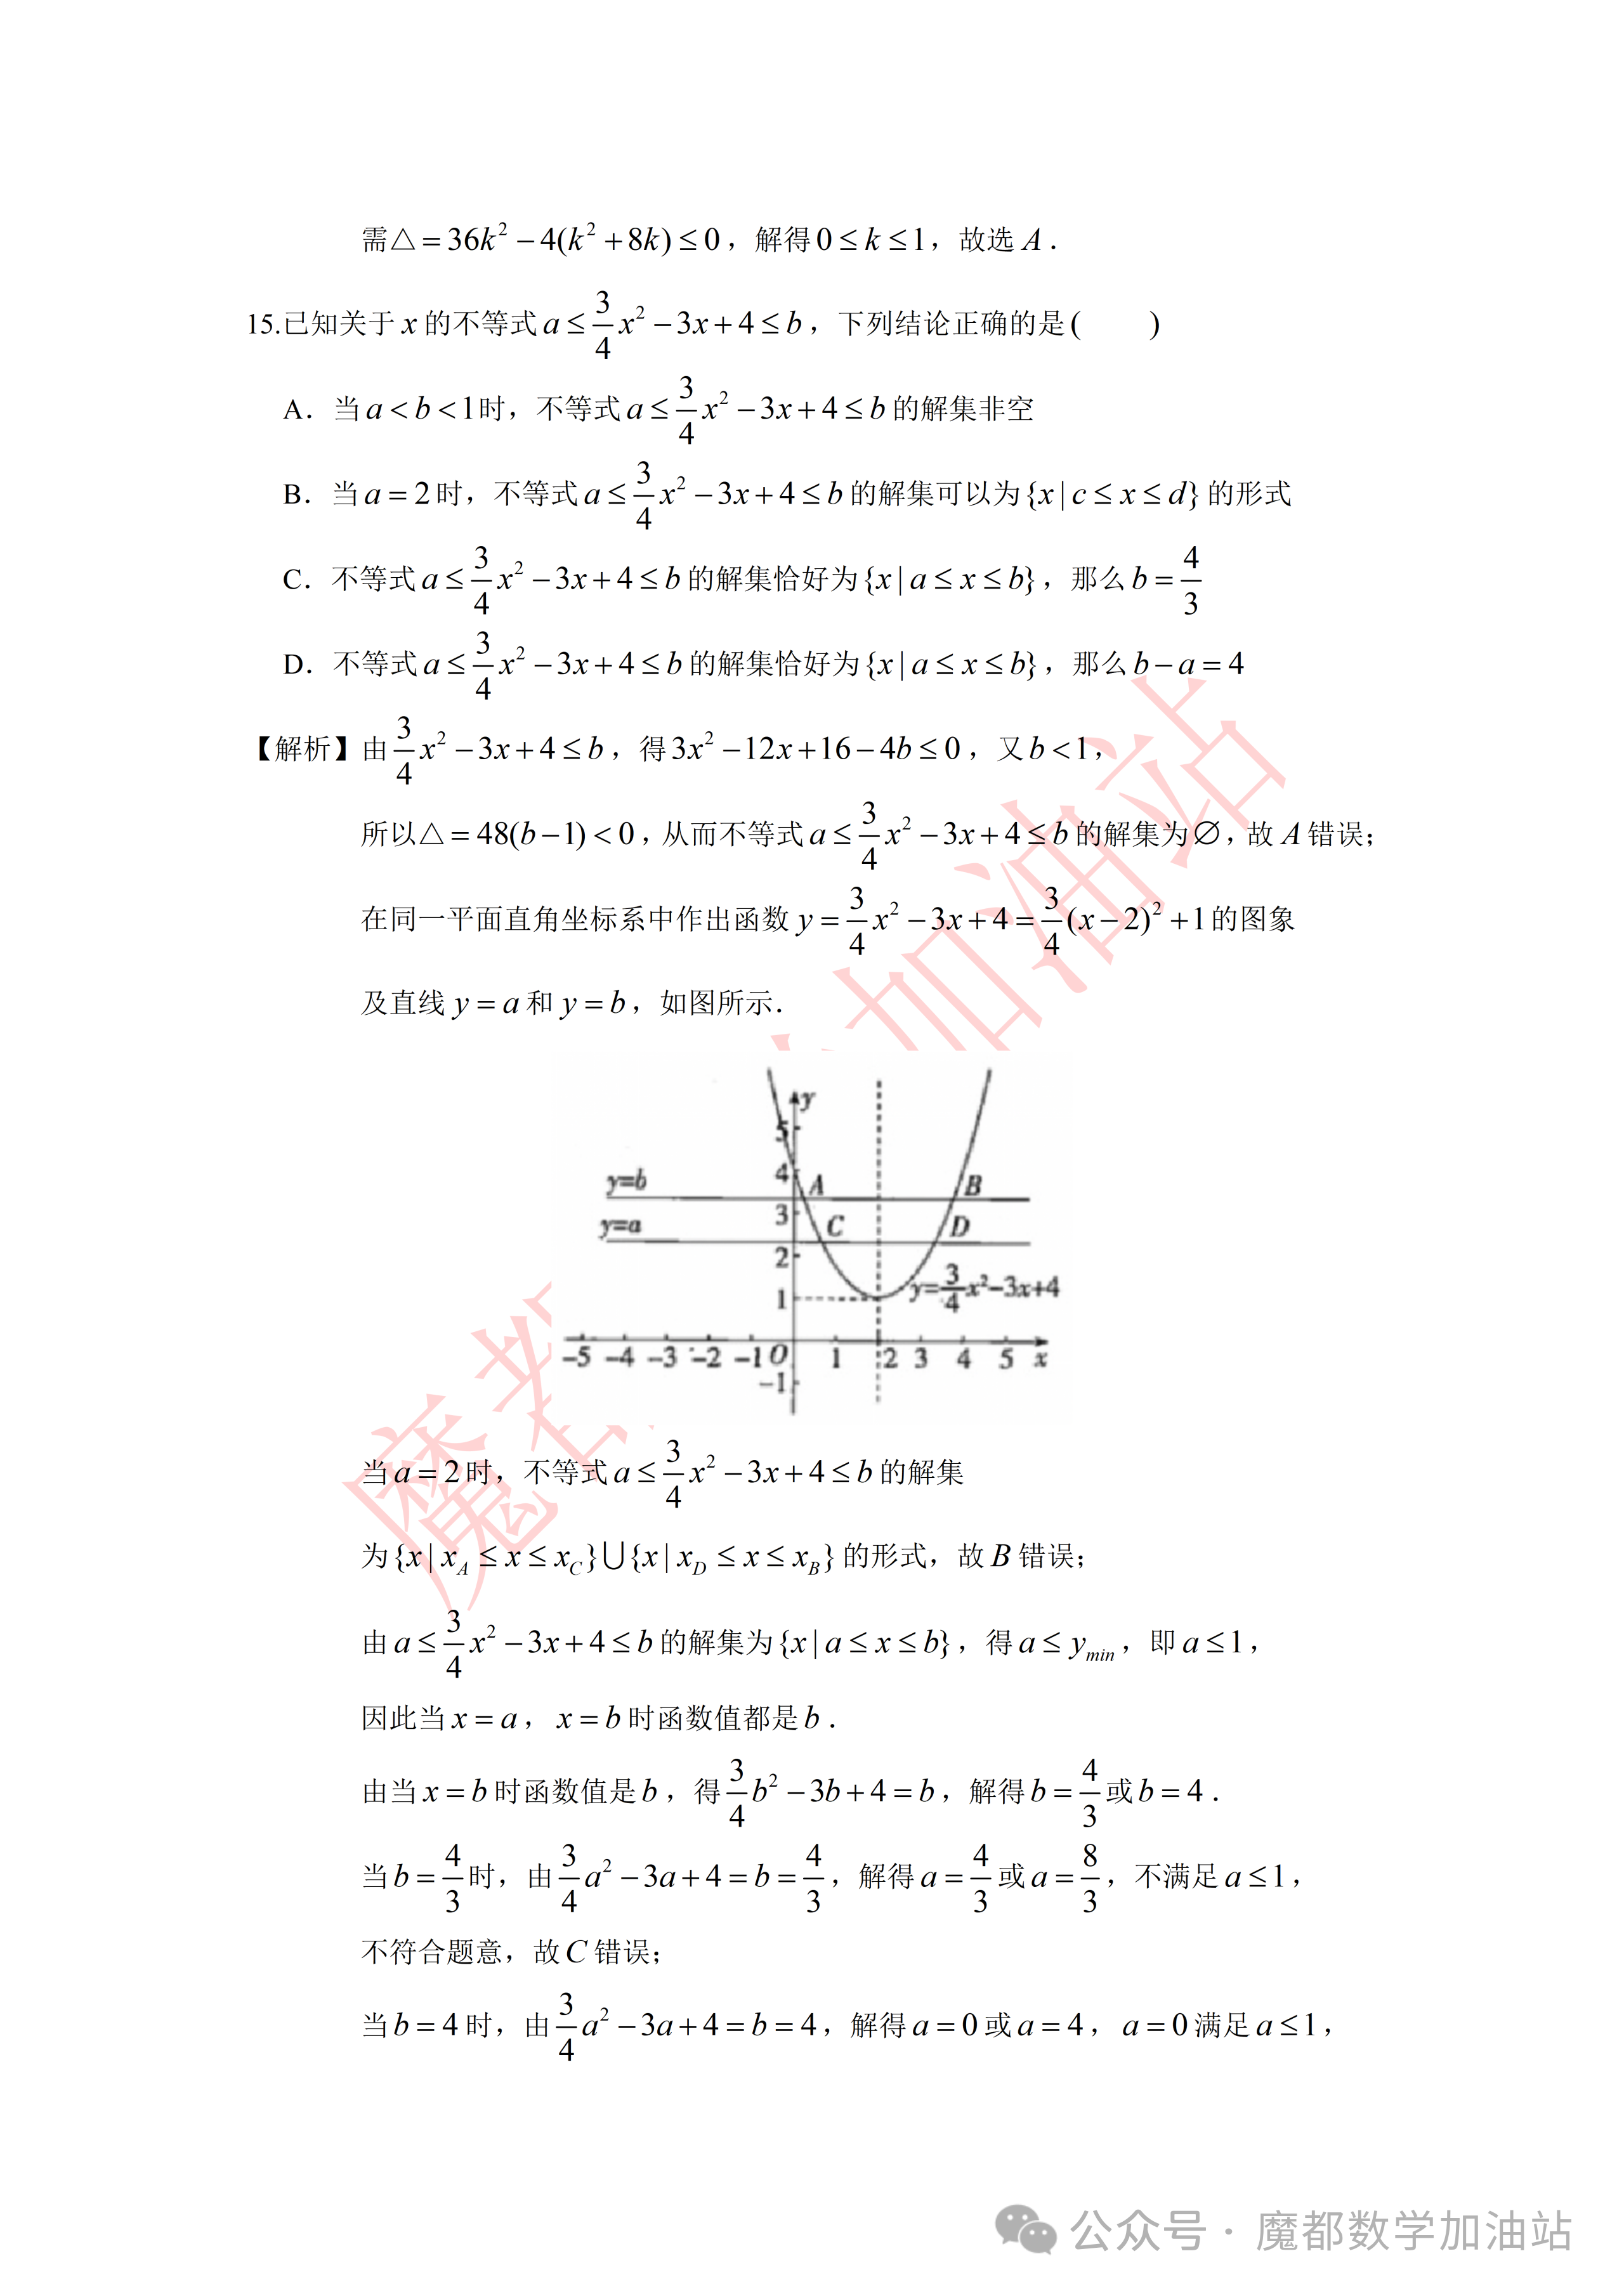
\includegraphics[width=.55\linewidth,trim=900bp 1400bp 760bp 1680bp,clip]{../原图/高一46_交附闵行_国庆作业3/05.png}
\end{center}
\step{当 $a=2$ 时，不等式 $a\leqslant\dfrac34x^2-3x+4\leqslant b$ 的解集为
$\{x\mid x_A\leqslant x\leqslant x_C\}\cup\{x\mid x_D\leqslant x\leqslant x_B\}$ 的形式，故 $B$ 错误；}
\step{由 $a\leqslant\dfrac34x^2-3x+4\leqslant b$ 的解集恰好为 $\{x\mid a\leqslant x\leqslant b\}$ 的形式，得 $a\leqslant y_{\min}$，即 $a\leqslant1$，}
\step{因为当 $x=a$、$x=b$ 时函数值都是 $b$，当 $x=a$ 时，$\dfrac34a^2-3a+4=b$；当 $x=b$ 时，$\dfrac34b^2-3b+4=b$，}
\step{解得 $b=\dfrac43$ 或 $b=4$，}
\step{当 $b=\dfrac43$ 时，由 $\dfrac34a^2-3a+4=b$，解得 $a=\dfrac43$ 或 $a=\dfrac83$，不符合题意，故 $C$ 错误；}
\step{当 $b=4$ 时，由 $\dfrac34a^2-3a+4=b$，解得 $a=0$ 或 $a=4$，$a=0$ 满足 $a\leqslant1$，故 $D$ 正确；}
\step{故选 $D$.}
\solend
\fi

\item 已知 $x$、$y\in(0,+\infty)$，则 $(x-y)^2+2y+1-x+\dfrac4x$ 的最小值为\mbox{（\quad）}

\keepwithprev
A. $1$\qquad B. $2$\qquad C. $3$\qquad D. $4$

\ans{$D$}

\ifanswer
\solbegin
\step{因为 $(x-y)^2+2y+1-x+\dfrac4x=(x-y-1)^2+x+\dfrac4x$，}
\step{当且仅当 $x-y-1=0$，且 $x=\dfrac4x$ 时取等号，}
\step{又因为 $x+\dfrac4x\geqslant2\sqrt{x\cdot\dfrac4x}=4$，当且仅当 $x=2$ 时取等号，}
\step{故选 $D$.}
\solend
\fi

\end{enumerate}

\bigsec{三、解答题}

\begin{enumerate}
\setcounter{enumi}{16}

\item 设集合 $A=\left\{x\middle|\dfrac{x-3}{x-1}<0\right\}$，$B=\{x\mid x^2-2ax+a^2-1>0\}$.
\begin{enumerate}[label=(\arabic*)]
\item 若 $a=3$，求 $A\cup B$；
\item 若“$x\in A$”是“$x\in B$”的充分条件，求实数 $a$ 的取值范围.
\end{enumerate}

\ifanswer
\solbegin
% 注：原卷题干为 a^2-1，故 a=3 时常数项为 8；题干与本步一致。
\stepm{(1)}{当 $a=3$ 时，$B=\{x\mid x^2-6x+8>0\}=\{x\mid x<2\text{ 或 }x>4\}$；}
\step{因为 $A=\left\{x\middle|\dfrac{x-3}{x-1}<0\right\}=\{x\mid(x-1)(x-3)<0\}=\{x\mid1<x<3\}$，}
\step{所以 $A\cup B=\{x\mid x<2\text{ 或 }x>4\}\cup\{x\mid1<x<3\}
=\{x\mid x<3\text{ 或 }x>4\}$.}
\stepm{(2)}{因为“$x\in A$”是“$x\in B$”的充分条件，所以 $A\subseteq B$，}
\step{因 $A=\left\{x\middle|\dfrac{x-3}{x-1}<0\right\}
=\{x\mid(x-1)(x-3)<0\}=\{x\mid1<x<3\}$，}
\step{所以 $A\subseteq B=\{x\mid x<a-1\text{ 或 }x>a+1\}$，}
\step{要使 $A\subseteq B$，需有 $a-1\geqslant3$ 或 $a+1\leqslant1$，}
\step{所以 $a\geqslant4$ 或 $a\leqslant0$，故 $a$ 的取值范围为 $\{a\mid a\geqslant4\text{ 或 }a\leqslant0\}$.}
\solend
\fi

\ansspace[6]

\item 某学校引入种植类劳动教育课程，打算围成如图所示的四块全等的长方形田地种植不同种类的蔬菜，其中一面可以利用原有的墙（足够长），其他各面需要用篱笆围成，设其中一块田地为矩形 $ABCD$.

\begin{center}
% 原图第 6 页配图直接裁取。
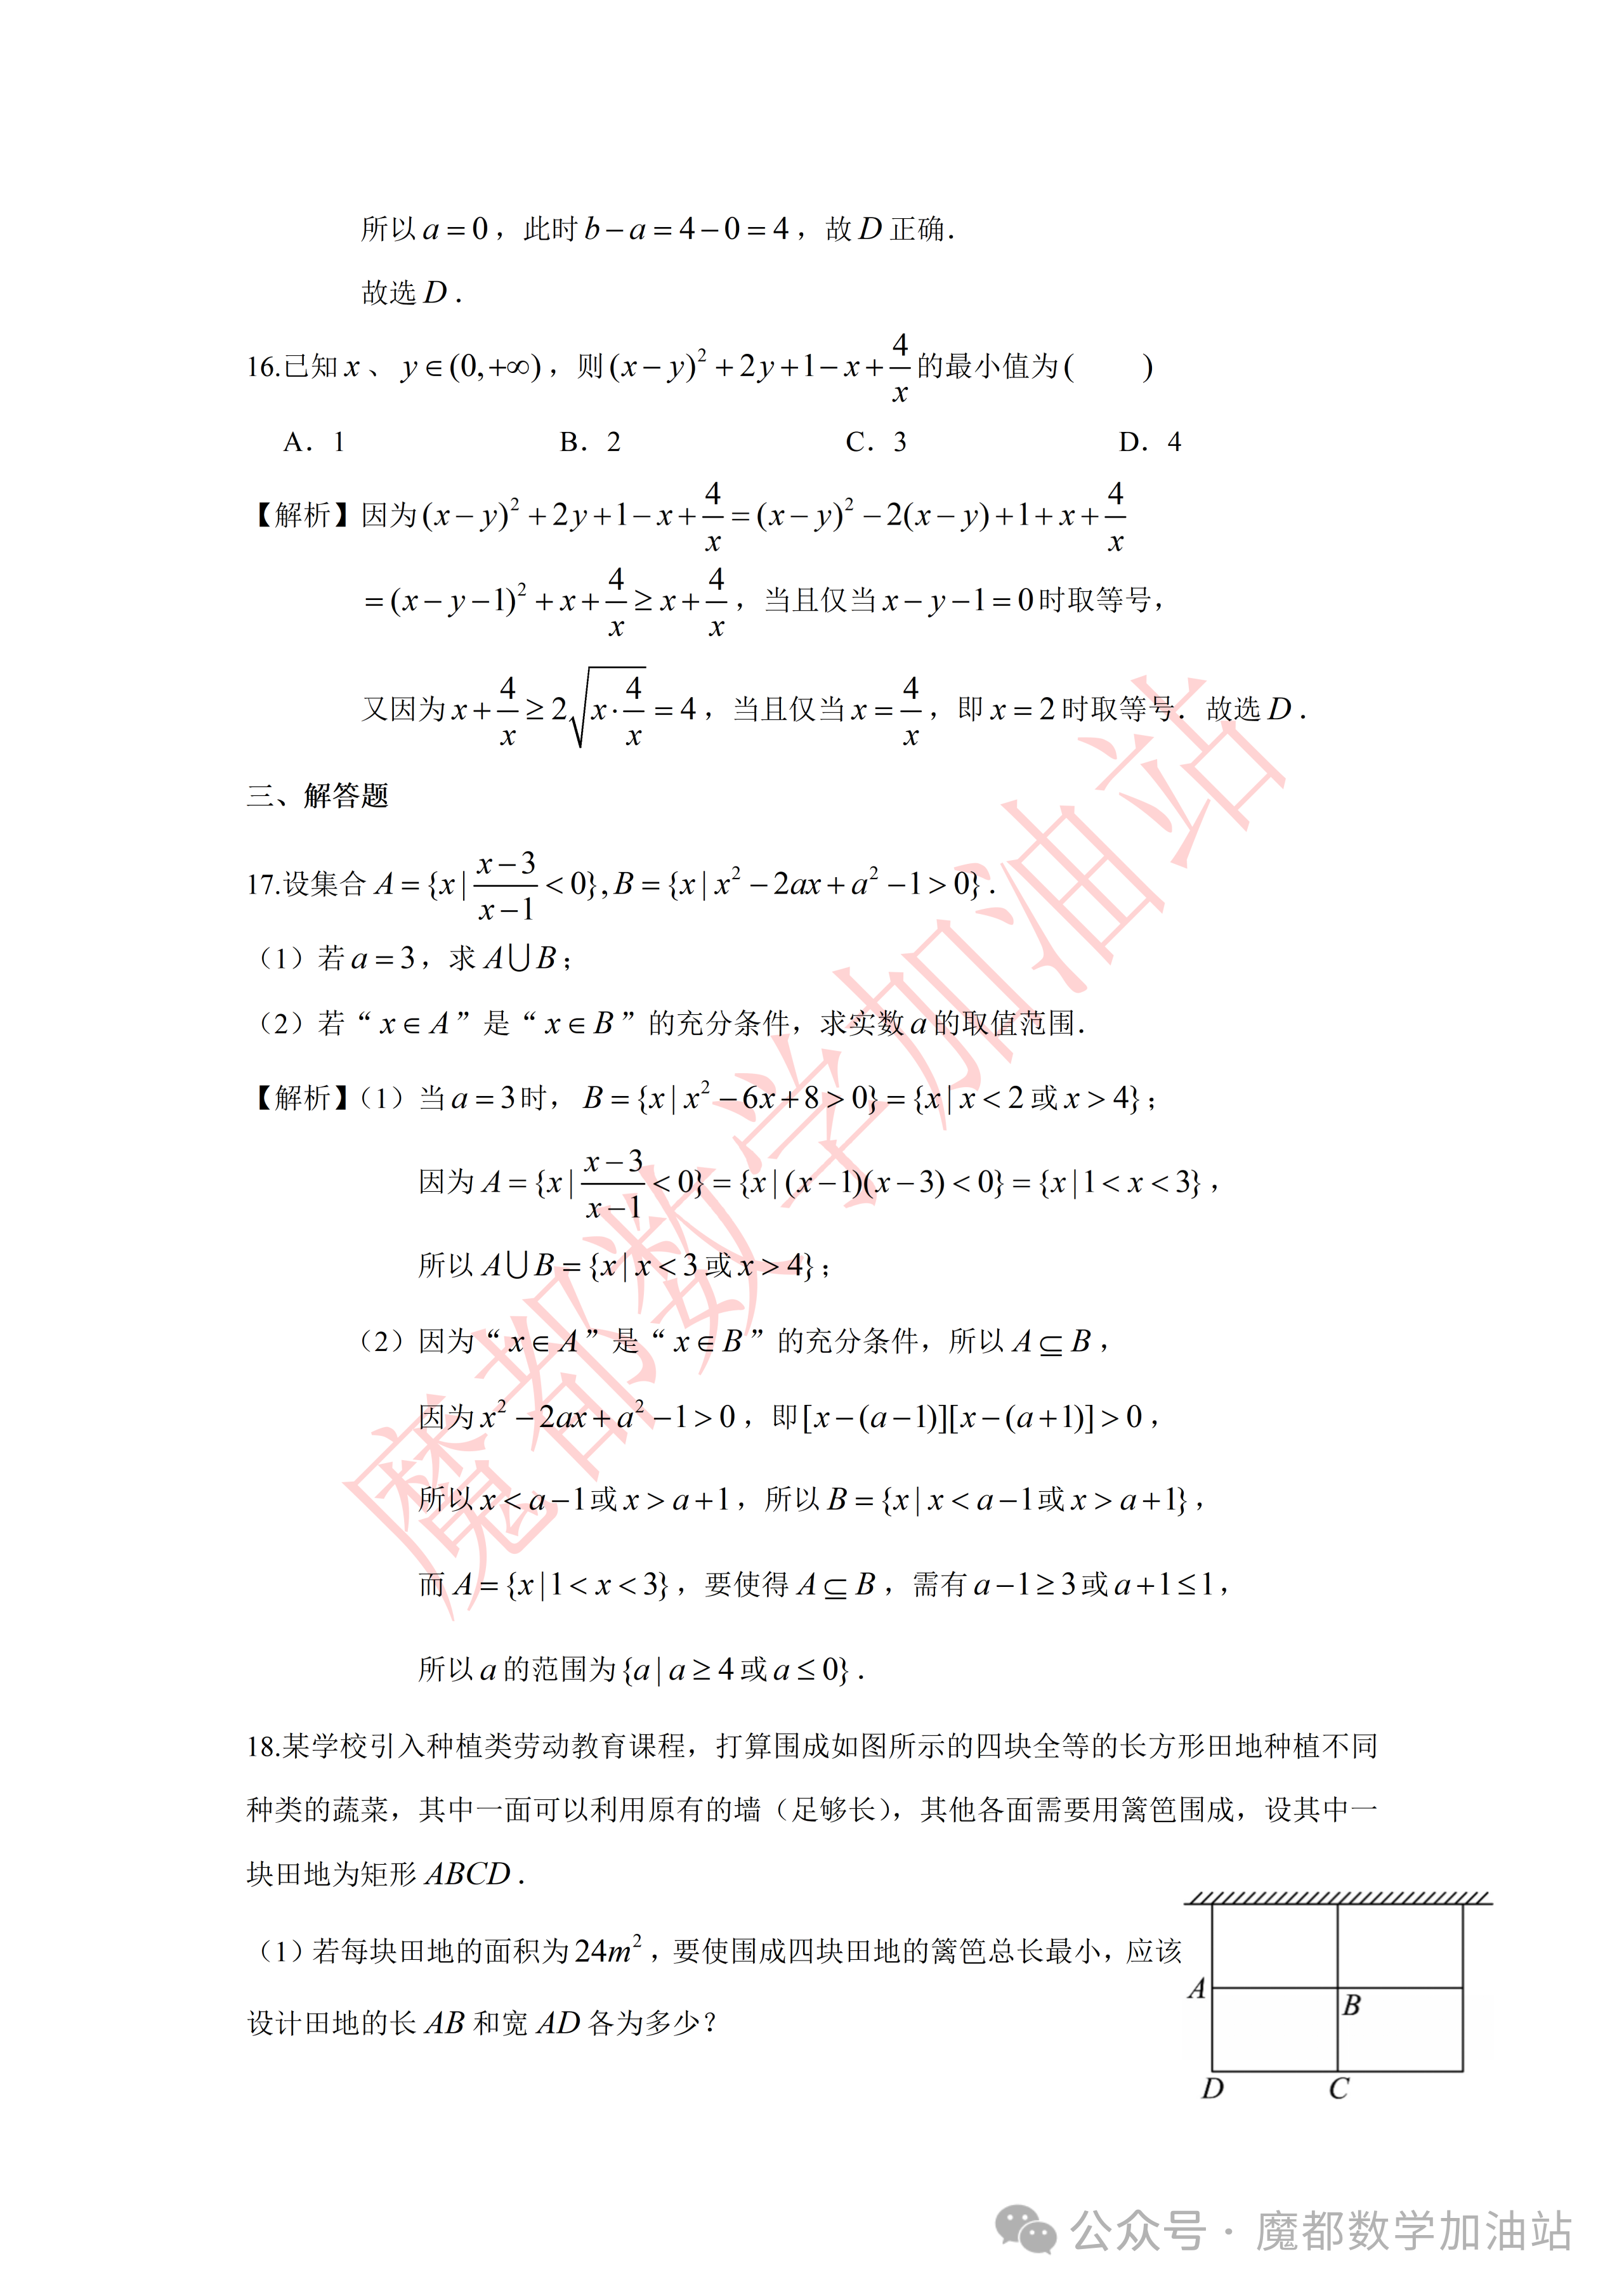
\includegraphics[width=.33\linewidth,trim=1866bp 220bp 210bp 2960bp,clip]{../原图/高一46_交附闵行_国庆作业3/06.png}
\end{center}

\begin{enumerate}[label=(\arabic*)]
\item 若每块田地的面积为 $24\,\text{m}^2$，要使围成四块田地的篱笆总长最小，应该设计田地的长 $AB$ 和宽 $AD$ 各为多少？
\item 现有 $40\,\text{m}$ 长的篱笆，要使每块田地的面积最大，应该设计田地的长 $AB$ 和宽 $AD$ 各为多少？
\end{enumerate}

\ifanswer
\solbegin
\stepm{(1)}{设 $AB$ 长为 $x\,\text{m}$，$AD$ 宽为 $y\,\text{m}$，由题意得 $xy=24$，篱笆总长为 $4x+6y$，}
\step{$4x+6y\geqslant2\sqrt{4x\cdot6y}=2\sqrt{24xy}=48$，}
\step{当且仅当 $4x=6y$ 时取等号，解得 $x=6$，$y=4$，}
\step{所以田地的长 $AB$ 为 $6\,\text{m}$，宽 $AD$ 为 $4\,\text{m}$.}
\stepm{(2)}{设 $AB$ 长为 $a\,\text{m}$，$AD$ 宽为 $b\,\text{m}$，由篱笆总长 $4a+6b=40$，即 $2a+3b=20$，}
\step{将 $a=\dfrac{20-3b}{2}$ 代入每块田地面积 $ab$，得 $ab=\dfrac12b(20-3b)=-\dfrac32b^2+10b$，}
\step{当 $b=\dfrac{10}{3}$ 时，$ab$ 最大，此时 $a=5$，}
\step{所以田地的长 $AB$ 为 $5\,\text{m}$，宽 $AD$ 为 $\dfrac{10}{3}\,\text{m}$.}
\solend
\fi

\ansspace[8]

\item 已知 $x_1$、$x_2$ 是一元二次方程 $4kx^2-4kx+k+1=0$ 的两个不等实数根.
\begin{enumerate}[label=(\arabic*)]
\item 若 $x_1$、$x_2$ 均为正根，求实数 $k$ 的取值范围；
\item 求使 $\dfrac{x_1}{x_2}+\dfrac{x_2}{x_1}-2$ 的值为整数 $k$ 的整数值.
\end{enumerate}

\ifanswer
\solbegin
\stepm{(1)}{由题意，$x_1$、$x_2$ 是方程 $4kx^2-4kx+k+1=0$ 的两个不等实数根，}
\step{故 $k\neq0$，$\Delta=(-4k)^2-16k(k+1)>0$，得 $-16k>0$，所以 $k<0$，}
\step{又 $x_1+x_2=1$，$x_1x_2=\dfrac{k+1}{4k}>0$，得 $k+1<0$，}
\step{所以 $k$ 的取值范围为 $(-\infty,-1)$.}
\stepm{(2)}{由题意，}
\step{$\dfrac{x_1}{x_2}+\dfrac{x_2}{x_1}-2
=\dfrac{x_1^2+x_2^2-2x_1x_2}{x_1x_2}
=\dfrac{(x_1+x_2)^2-4x_1x_2}{x_1x_2}$，}
\step{又 $x_1+x_2=1$，$x_1x_2=\dfrac{k+1}{4k}$，}
\step{则 $\dfrac{x_1}{x_2}+\dfrac{x_2}{x_1}-2=-\dfrac4{k+1}$，}
\step{由于 $-\dfrac4{k+1}$ 为整数，故 $k+1$ 只能取 $\pm1$、$\pm2$、$\pm4$，又 $k<-1$，}
\step{所以整数 $k$ 的值为 $-2$、$-3$、$-5$.}
\solend
\fi

\ansspace[8]

\item 已知 $a>0$，$b>0$，且 $2a+3b=3$.
\begin{enumerate}[label=(\arabic*)]
\item 求 $ab$ 的最大值；
\item 求 $a-\dfrac1{6b}$ 的最大值；
\item 求 $\dfrac2a+\dfrac3{b+1}$ 的最小值.
\end{enumerate}

\ifanswer
\solbegin
\stepm{(1)}{由 $2a+3b=3$，得 $3=2a+3b\geqslant2\sqrt{6ab}$，}
\step{所以 $ab\leqslant\dfrac38$，当且仅当 $2a=3b=\dfrac32$ 时取等号，}
\step{故 $ab$ 的最大值为 $\dfrac38$.}
\stepm{(2)}{由 $2a+3b=3$，得 $a=\dfrac32-\dfrac32b$，}
\step{则 $a-\dfrac1{6b}=\dfrac32-\dfrac32b-\dfrac1{6b}$，}
\step{由基本不等式，$\dfrac32b+\dfrac1{6b}\geqslant2\sqrt{\dfrac32b\cdot\dfrac1{6b}}=1$，}
\step{当且仅当 $\dfrac32b=\dfrac1{6b}$，即 $b=\dfrac13$、$a=1$ 时取等号，}
\step{所以 $a-\dfrac1{6b}$ 的最大值为 $\dfrac12$.}
\stepm{(3)}{由 $2a+3b=3$，得 $2a+3(b+1)=6$，}
\step{$\dfrac2a+\dfrac3{b+1}
=\dfrac16\left(2a+3(b+1)\right)\left(\dfrac2a+\dfrac3{b+1}\right)$}
\step{$=\dfrac16\left(13+\dfrac{6(b+1)}a+\dfrac{6a}{b+1}\right)
\geqslant\dfrac16\left(13+2\sqrt{\dfrac{6(b+1)}a\cdot\dfrac{6a}{b+1}}\right)=\dfrac{25}{6}$，}
\step{当且仅当 $a=b+1$，即 $a=\dfrac65$、$b=\dfrac15$ 时取等号，}
\step{所以 $\dfrac2a+\dfrac3{b+1}$ 的最小值为 $\dfrac{25}{6}$.}
\solend
\fi

\ansspace[8]

\item 已知 $U=\R$ 为全集，集合 $A=\{s^2+3t^2\mid s,t\in U\}$.
\begin{enumerate}[label=(\arabic*)]
\item 设 $U=\{1,3,5\}$，求集合 $A$ 的元素个数；
\item 设 $U=\Z$，证明：若 $x\in A$，则 $7x\in A$；
\item 设 $U=\R$，$x$、$y\in A$，且 $x=m^2+3n^2$，$y=p^2+3q^2$，若 $mp-3nq=\sqrt3$，求 $x+y+mq+np$ 的最小值.
\end{enumerate}

\ifanswer
\solbegin
\stepm{(1)}{当 $s=1$，$t=1$ 时，$s^2+3t^2=1+3=4$；}
\step{当 $s=1$，$t=3$ 时，$s^2+3t^2=1+27=28$；}
\step{当 $s=1$，$t=5$ 时，$s^2+3t^2=1+75=76$；}
\step{当 $s=3$，$t=1$ 时，$s^2+3t^2=9+3=12$；}
\step{当 $s=3$，$t=3$ 时，$s^2+3t^2=9+27=36$；}
\step{当 $s=3$，$t=5$ 时，$s^2+3t^2=9+75=84$；}
\step{当 $s=5$，$t=1$ 时，$s^2+3t^2=25+3=28$；}
\step{当 $s=5$，$t=3$ 时，$s^2+3t^2=25+27=52$；}
\step{当 $s=5$，$t=5$ 时，$s^2+3t^2=25+75=100$，}
\step{所以 $A=\{4,12,28,36,52,76,84,100\}$，有 $8$ 个元素.}
\stepm{(2)}{因为 $U=\Z$，$x\in A$，设 $x=s^2+3t^2$，}
\step{则 $7x=7(s^2+3t^2)=(2s+3t)^2+3(s-2t)^2\in A$，}
\step{所以 $7x\in A$.}
\stepm{(3)}{因为 $x=m^2+3n^2$，$y=p^2+3q^2$，}
\step{$xy=(m^2+3n^2)(p^2+3q^2)=3(mq+np)^2+(mp-3nq)^2$，}
\step{设 $mq+np=b$，则 $xy=3b^2+3$，所以 $y=\dfrac{3b^2+3}{x}$，}
\step{于是 $x+y+mq+np=x+\dfrac{3b^2+3}{x}+b\geqslant2\sqrt{3b^2+3}+b$，}
\step{设 $2\sqrt{3b^2+3}+b=t$，整理得 $11b^2+2bt+12-t^2=0$，}
\step{判别式法，$\Delta=4t^2-44(12-t^2)\geqslant0$，得 $t\geqslant\sqrt{11}$，}
\step{即 $(x+y+mq+np)_{\min}=\sqrt{11}$，所以 $x+y+mq+np$ 的最小值为 $\sqrt{11}$.}
\solend
\fi

\ansspace*[10]

\end{enumerate}

\end{document}
"
% 紧凑版：xelatex "\def\iscompact{1}% 高一46_交附闵行_国庆作业3.tex
%   —— 高一上数学“2026-2027 年交附闵行高一上国庆作业 3”（讲评版）
% 试卷版：xelatex 高一46_交附闵行_国庆作业3.tex
% 答案版：xelatex "\def\isanswer{1}\input{高一46_交附闵行_国庆作业3.tex}"
% 紧凑版：xelatex "\def\iscompact{1}\input{高一46_交附闵行_国庆作业3.tex}"
%
% 原始材料：微信公众号“魔都数学加油站”，作者破晓，2026-10-02 17:56 发布。
% 原文标题：“27学年高一46——2026-2027你那上海市交附闵行高一上国庆作业3”
% （公众号标题中的“你那”照录，系原文标题字样）；原文链接：
% http://mp.weixin.qq.com/s?__biz=Mzg4ODU1ODMxOQ==&mid=2247591657&idx=3&sn=a894d1a16611283a61b3eaba32a3f24c&chksm=cee83366c6a55381b370069f84ef63d20251f94608bb37cc4ec2d66227401bd147f4f6bd8256&scene=126&sessionid=1790935402&subscene=7&clicktime=1790937618&enterid=1790937618#rd
% 正文为 9 张 PNG 页，按页序读取原图；第 01、02、07 页 4762×6735，
% 第 03—06、08、09 页 2560×3620。卷面标题照原卷印作“2026-2027 年交附闵行高一上国庆作业 3”。
% 原文从第 3 题起，题号照原卷保留；正文为讲评版，答案、解析依原卷顺序录入。
% 水印及页脚公众号标识不录入。卷面插图直接裁取对应原图页，不另制图片文件。
%
% 与原卷的排版差异：
%   ① 原卷按“一、填空题”“二、选择题”“三、解答题”分节，本稿沿用原节与原题号，
%      只改排为全稿统一的大节样式；
%   ② 原卷答案与解析依页面位置分布，本稿按 common.sty 统一置于答案版；
%   ③ 原卷副标题未印，本稿按“知识模块”口径标作“集合与常用逻辑用语、不等式”。
%
% 原卷存疑一处（照抄未改，见第 12 题题干及解析处注释）：
%   第 12 题题干同时给出 x∈Z，却称不等式组有“50 个不等的实数解”；解析按整数根计数。
%   此处题干与解析的原文不一致，本稿均照录。
% 第 17 题曾疑似有常数项不一致：复核原图题干为 a^2-1，a=3 时常数项确为 8，
% 与解析相符；不将其记作原卷错误。
%
\documentclass[a4paper,11pt]{article}
\usepackage{common}

\begin{document}

\examtitlest[3]{2026--2027 年交附闵行高一上国庆作业 3}{集合与常用逻辑用语、不等式}

\bigsec{一、填空题}

\begin{enumerate}
\setcounter{enumi}{2}

\item 不等式 $\dfrac{x^2-10}{x+2}\geqslant1$ 的解集为\blankline[4.4em].

\ifanswer
\ans{$\{x\mid-3\leqslant x<-2\text{ 或 }x\geqslant4\}$}
\solbegin
\step{不等式 $\dfrac{x^2-10}{x+2}\geqslant1$，移项得 $\dfrac{x^2-10}{x+2}-1\geqslant0$，}
\step{通分得 $\dfrac{x^2-x-12}{x+2}\geqslant0$，即 $\dfrac{(x-4)(x+3)}{x+2}\geqslant0$，}
\step{解得 $-3\leqslant x<-2$ 或 $x\geqslant4$，}
\step{故不等式的解集为 $\{x\mid-3\leqslant x<-2\text{ 或 }x\geqslant4\}$.}
\solend
\fi

\item $|x-3|+|x-5|\geqslant2$，当等号成立时，$x$ 的范围是\blankline[4.4em].

\ifanswer
\ans{$[3,5]$}
\fi

\item 若直角三角形斜边长等于 $4\sqrt2\,\text{cm}$，则直角三角形面积的最大值为\blankline[4.4em].

\ifanswer
\solbegin
\step{设 $Rt\triangle ABC$ 中，$C=90^\circ$，则 $c=\sqrt{a^2+b^2}=4\sqrt2$，所以 $a^2+b^2=32$，}
\step{由基本不等式得 $a^2+b^2\geqslant2ab$，当且仅当 $a=b=4$ 时取等号，}
\step{所以 $\triangle ABC$ 的面积 $S=\dfrac12ab\leqslant8$，}
\step{当且仅当 $a=b=4$ 时，$\triangle ABC$ 的面积最大值为 $8$.}
\solend
\fi

\item 不等式 $(x-1)(2-x)>0$ 的解集为\blankline[4.4em].

\ifanswer
\solbegin
\step{$(x-1)(2-x)>0\Rightarrow(x-1)(x-2)<0$，}
\step{故不等式的解集为 $\{x\mid1<x<2\}$.}
\solend
\fi

\item 已知集合 $A=\{1,2\}$，$B=\{x\mid x^2-2mx+m=0\}$，$A\cup B=A$，则实数 $m$ 的取值范围为\blankline[4.4em].

\ifanswer
\solbegin
\step{因为 $A\cup B=A$，所以 $B\subseteq A$，}
\step{当 $B=\varnothing$ 时，$\Delta=(-2m)^2-4m<0$，解得 $0<m<1$，}
\step{当 $B$ 为单元素集时，$\Delta=0$，解得 $m=0$ 或 $m=1$，}
\step{当 $m=0$ 时，方程 $x^2=0$，解得 $x=0$，此时 $B=\{0\}$，不满足 $B\subseteq A$；}
\step{当 $m=1$ 时，方程 $x^2-2x+1=0$，解得 $x=1$，此时 $B=\{1\}$，满足 $B\subseteq A$；}
\step{当 $B=\{1,2\}$ 时，由韦达定理得 $1+2=2m$，$1\times2=m$，无解，}
\step{综上所述，实数 $m$ 的取值范围为 $\{m\mid0<m\leqslant1\}$.}
\solend
\fi

\item 设 $a$、$b$、$c\in\R^+$，若 $a+b+c=1$，则 $\dfrac1a+\dfrac1b+\dfrac1c\geqslant$\blankline[4.4em].

\ifanswer
\solbegin
\step{因为 $a$、$b$、$c\in\R^+$，且 $a+b+c=1$，}
\step{所以 $\dfrac1a+\dfrac1b+\dfrac1c=(a+b+c)\left(\dfrac1a+\dfrac1b+\dfrac1c\right)$}
\step{$=3+\dfrac ab+\dfrac ba+\dfrac ac+\dfrac ca+\dfrac bc+\dfrac cb$，}
\step{由基本不等式得 $\dfrac ab+\dfrac ba\geqslant2$，$\dfrac ac+\dfrac ca\geqslant2$，$\dfrac bc+\dfrac cb\geqslant2$，}
\step{所以 $\dfrac1a+\dfrac1b+\dfrac1c\geqslant9$，当且仅当 $a=b=c=\dfrac13$ 时取等号，}
\step{所以 $\dfrac1a+\dfrac1b+\dfrac1c$ 的最小值为 $9$.}
\solend
\fi

\item 已知 $-1\leqslant x+y\leqslant2$，$-2\leqslant x-y\leqslant1$，则 $x-2y$ 的范围为\blankline[4.4em].

\ifanswer
\solbegin
\step{设 $x-2y=m(x+y)+n(x-y)$，}
\step{则 $x-2y=(m+n)x+(m-n)y$，所以 $m+n=1$，$m-n=-2$，}
\step{解得 $m=-\dfrac12$，$n=\dfrac32$，}
\step{所以 $x-2y=-\dfrac12(x+y)+\dfrac32(x-y)$，}
\step{因为 $-1\leqslant x+y\leqslant2$，$-2\leqslant x-y\leqslant1$，}
\step{所以 $-4\leqslant x-2y\leqslant2$，即 $x-2y$ 的范围为 $[-4,2]$.}
\solend
\fi

\item 设集合 $A=\{1,2,m\}$，其中 $m$ 为实数，令 $B=\{a^2\mid a\in A\}$，$C=A\cup B$. 若 $C$ 中所有元素之和为 $6$，则 $C$ 中的所有元素之积为\blankline[4.4em].

\ifanswer
\solbegin
\step{因为 $A=\{1,2,m\}$，所以 $B=\{a^2\mid a\in A\}=\{1,4,m^2\}$，$m\neq1$，$m\neq2$，}
\step{又 $C=A\cup B$，所以 $1\in C$，$4\in C$，$m^2\in C$，}
\step{若 $m^2=1$，则 $m=-1$ 或 $m=1$（舍），当 $m=-1$ 时，$C=\{1,2,4,-1\}$，$C$ 中所有元素之和为 $6$，}
\step{此时 $C$ 中所有元素之积为 $-8$；}
\step{若 $m^2=2$，则 $m=-\sqrt2$ 或 $m=\sqrt2$，$C$ 中所有元素之和不符合题意；}
\step{若 $m^2=4$，则 $m=-2$ 或 $m=2$，此时 $C=\{1,2,4,-2\}$ 或 $C=\{1,2,4\}$，所有元素之和不符合题意；}
\step{若 $m^2\neq1$，$m^2\neq2$，$m^2\neq4$，则 $C=\{1,2,4,m,m^2\}$，}
\step{所以 $1+2+4+m+m^2=6$，即 $m^2+m+1=0$，无解，}
\step{综上所述，$C$ 中所有元素之积为 $-8$.}
\solend
\fi

\item 若对任意实数 $x>0$，$y>0$，不等式 $x+\sqrt{xy}\leqslant a(x+y)$ 恒成立，则实数 $a$ 的最小值为\blankline[4.4em].

\ifanswer
\solbegin
\step{由不等式 $x+\sqrt{xy}\leqslant a(x+y)$ 对任意实数 $x>0$，$y>0$ 恒成立，}
\step{得 $a\geqslant\dfrac{x+\sqrt{xy}}{x+y}$，}
\step{设 $\sqrt{\dfrac yx}=t>0$，则 $a\geqslant\dfrac{1+t}{1+t^2}$，}
\step{$\dfrac{1+t}{1+t^2}\leqslant\dfrac{\sqrt2+1}{2}$，当且仅当 $t=\sqrt2-1$ 时取等号，}
\step{所以实数 $a$ 的最小值为 $\dfrac{\sqrt2+1}{2}$.}
\solend
\fi

% 注：原卷题干给出 x∈Z，却写“实数解”；解析按整数解计数，题干与解析不一致，照录未改。
\item 若关于 $x$ 的不等式组
$\begin{cases}x^2-3mx\geqslant4m^2\\-20<x<120\end{cases}$（$x\in\Z,m>0$）恰有 $50$ 个不等的实数解，则 $m$ 的取值范围为\blankline[4.4em]（结果用区间表示）.

\ifanswer
\solbegin
\step{由 $x^2-3mx\geqslant4m^2$ 以及 $m>0$，解得 $x\leqslant-m$ 或 $x\geqslant4m$，}
\step{由原不等式组恰有 $50$ 个不等的实数解，可画出如下解集区间：}
\begin{center}
% 原图第 4 页数轴图直接裁取。
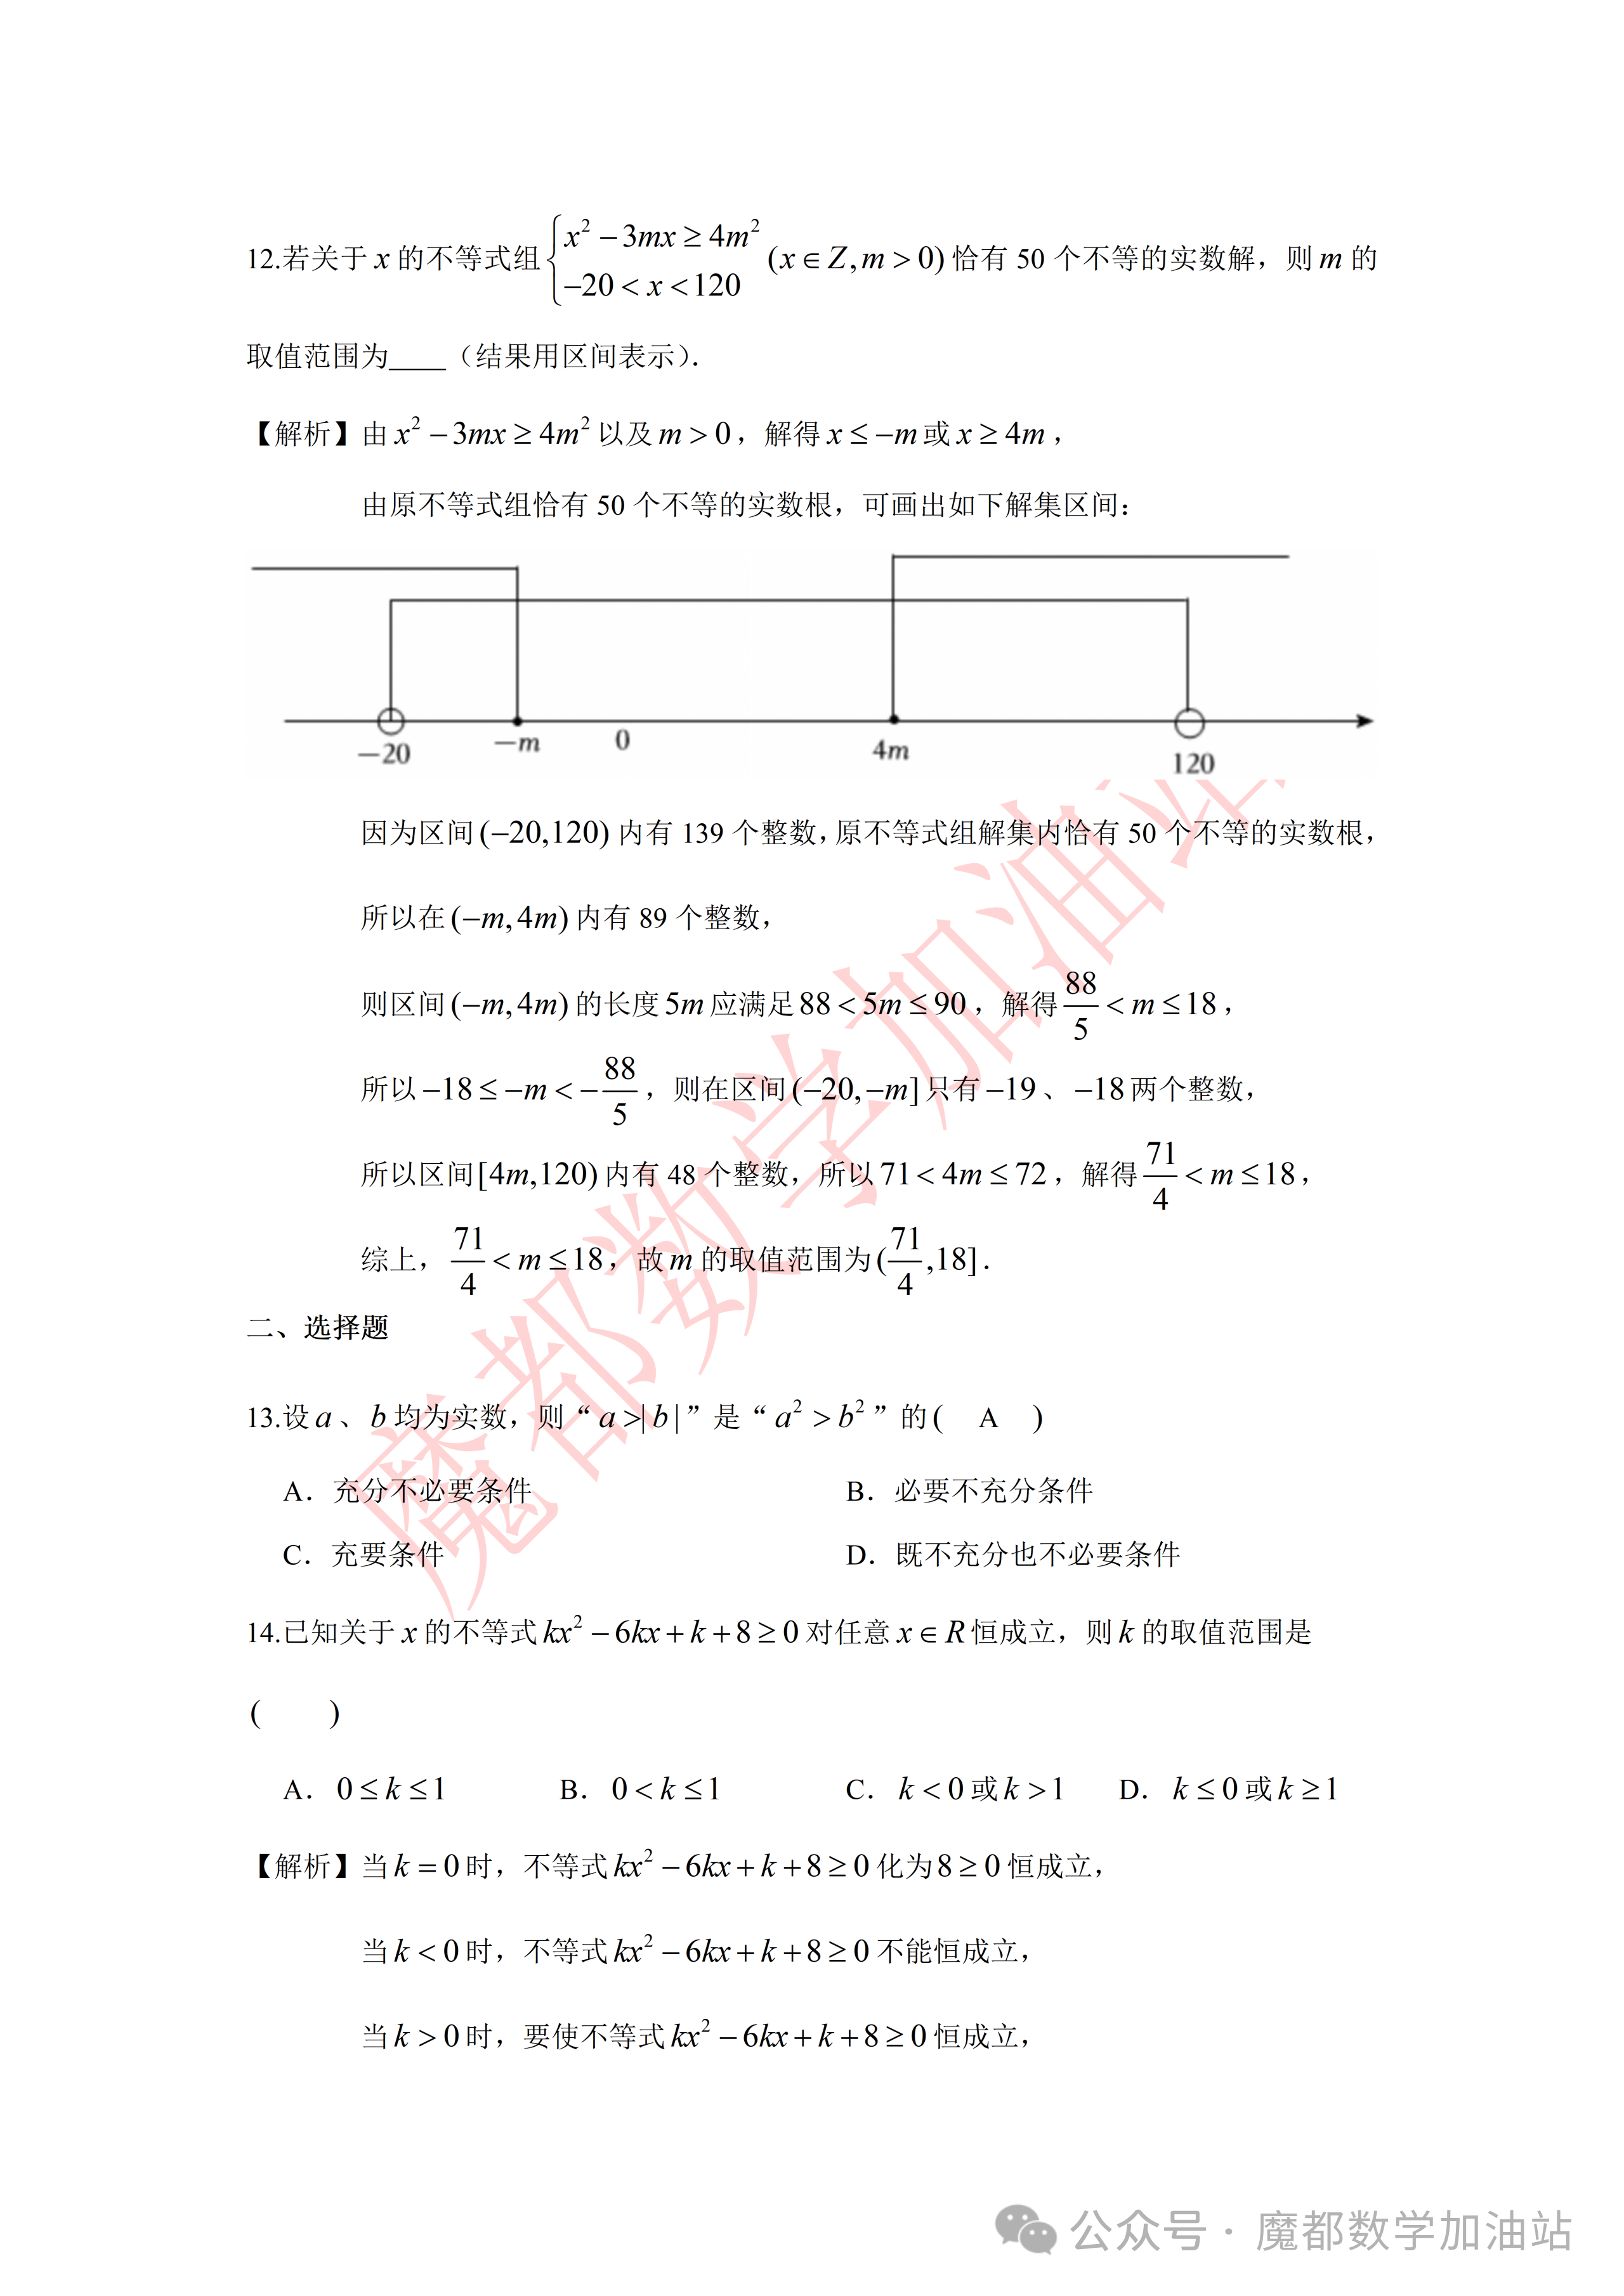
\includegraphics[width=.88\linewidth,trim=400bp 2410bp 320bp 860bp,clip]{../原图/高一46_交附闵行_国庆作业3/04.png}
\end{center}
\step{因为区间 $(-20,120)$ 内有 $139$ 个整数，原不等式组解集内有 $50$ 个不等的整数根，}
\step{所以在区间 $(-m,4m)$ 内有 $89$ 个整数，}
\step{则区间 $(-m,4m)$ 的长度 $5m$ 应满足 $88<5m\leqslant90$，解得 $\dfrac{88}{5}<m\leqslant18$，}
% 注：原卷题干称“实数解”，本行及后文按原卷解析照录为整数根计数。
\step{所以 $-18\leqslant-m<-\dfrac{88}{5}$，则在区间 $(-20,-m]$ 内有 $-19$、$-18$ 两个整数，}
\step{所以区间 $[4m,120)$ 内有 $48$ 个整数，}
\step{则 $71<4m\leqslant72$，解得 $\dfrac{71}{4}<m\leqslant18$，}
\step{综上，$\dfrac{71}{4}<m\leqslant18$，故 $m$ 的取值范围为 $\left(\dfrac{71}{4},18\right]$.}
\solend
\fi

\end{enumerate}

\bigsec{二、选择题}

\begin{enumerate}
\setcounter{enumi}{12}

\item 设 $a$、$b$ 均为实数，则“$a>|b|$”是“$a^2>b^2$”的\mbox{（\quad）}

\keepwithprev
A. 充分不必要条件\qquad B. 必要不充分条件

C. 充要条件\qquad\qquad D. 既不充分也不必要条件

\ans{$A$}

\item 已知关于 $x$ 的不等式 $kx^2-6kx+k+8\geqslant0$ 对任意 $x\in\R$ 恒成立，则 $k$ 的取值范围是\mbox{（\quad）}

\keepwithprev
A. $0\leqslant k\leqslant1$\qquad B. $0<k\leqslant1$

C. $k<0$ 或 $k>1$\qquad D. $k\leqslant0$ 或 $k\geqslant1$

\ans{$A$}

\ifanswer
\solbegin
\step{当 $k=0$ 时，不等式 $kx^2-6kx+k+8\geqslant0$ 化为 $8\geqslant0$ 恒成立，}
\step{当 $k<0$ 时，不等式 $kx^2-6kx+k+8\geqslant0$ 不能恒成立，}
\step{当 $k>0$ 时，要使不等式 $kx^2-6kx+k+8\geqslant0$ 恒成立，}
\step{需 $\Delta=36k^2-4(k^2+8k)\leqslant0$，解得 $0\leqslant k\leqslant1$，故选 $A$.}
\solend
\fi

\item 已知关于 $x$ 的不等式 $a\leqslant\dfrac34x^2-3x+4\leqslant b$，下列结论正确的是\mbox{（\quad）}

\keepwithprev
A. 当 $a<b<1$ 时，不等式 $a\leqslant\dfrac34x^2-3x+4\leqslant b$ 的解集非空

B. 当 $a=2$ 时，不等式 $a\leqslant\dfrac34x^2-3x+4\leqslant b$ 的解集可以为 $\{x\mid c\leqslant x\leqslant d\}$ 的形式

C. 不等式 $a\leqslant\dfrac34x^2-3x+4\leqslant b$ 的解集恰好为 $\{x\mid a\leqslant x\leqslant b\}$，那么 $b=\dfrac43$

D. 不等式 $a\leqslant\dfrac34x^2-3x+4\leqslant b$ 的解集恰好为 $\{x\mid a\leqslant x\leqslant b\}$，那么 $b-a=4$

\ans{$D$}

\ifanswer
\solbegin
\step{由 $\dfrac34x^2-3x+4\leqslant b$，得 $3x^2-12x+16-4b\leqslant0$，又 $b<1$，}
\step{所以 $\Delta=144-12(16-4b)=48(b-1)<0$，从而不等式无解，故 $A$ 错误；}
\step{在同一平面直角坐标系中作出函数 $y=\dfrac34x^2-3x+4=\dfrac34(x-2)^2+1$ 的图象及直线 $y=a$ 和 $y=b$，如图所示.}
\begin{center}
% 原图第 5 页解析配图直接裁取。
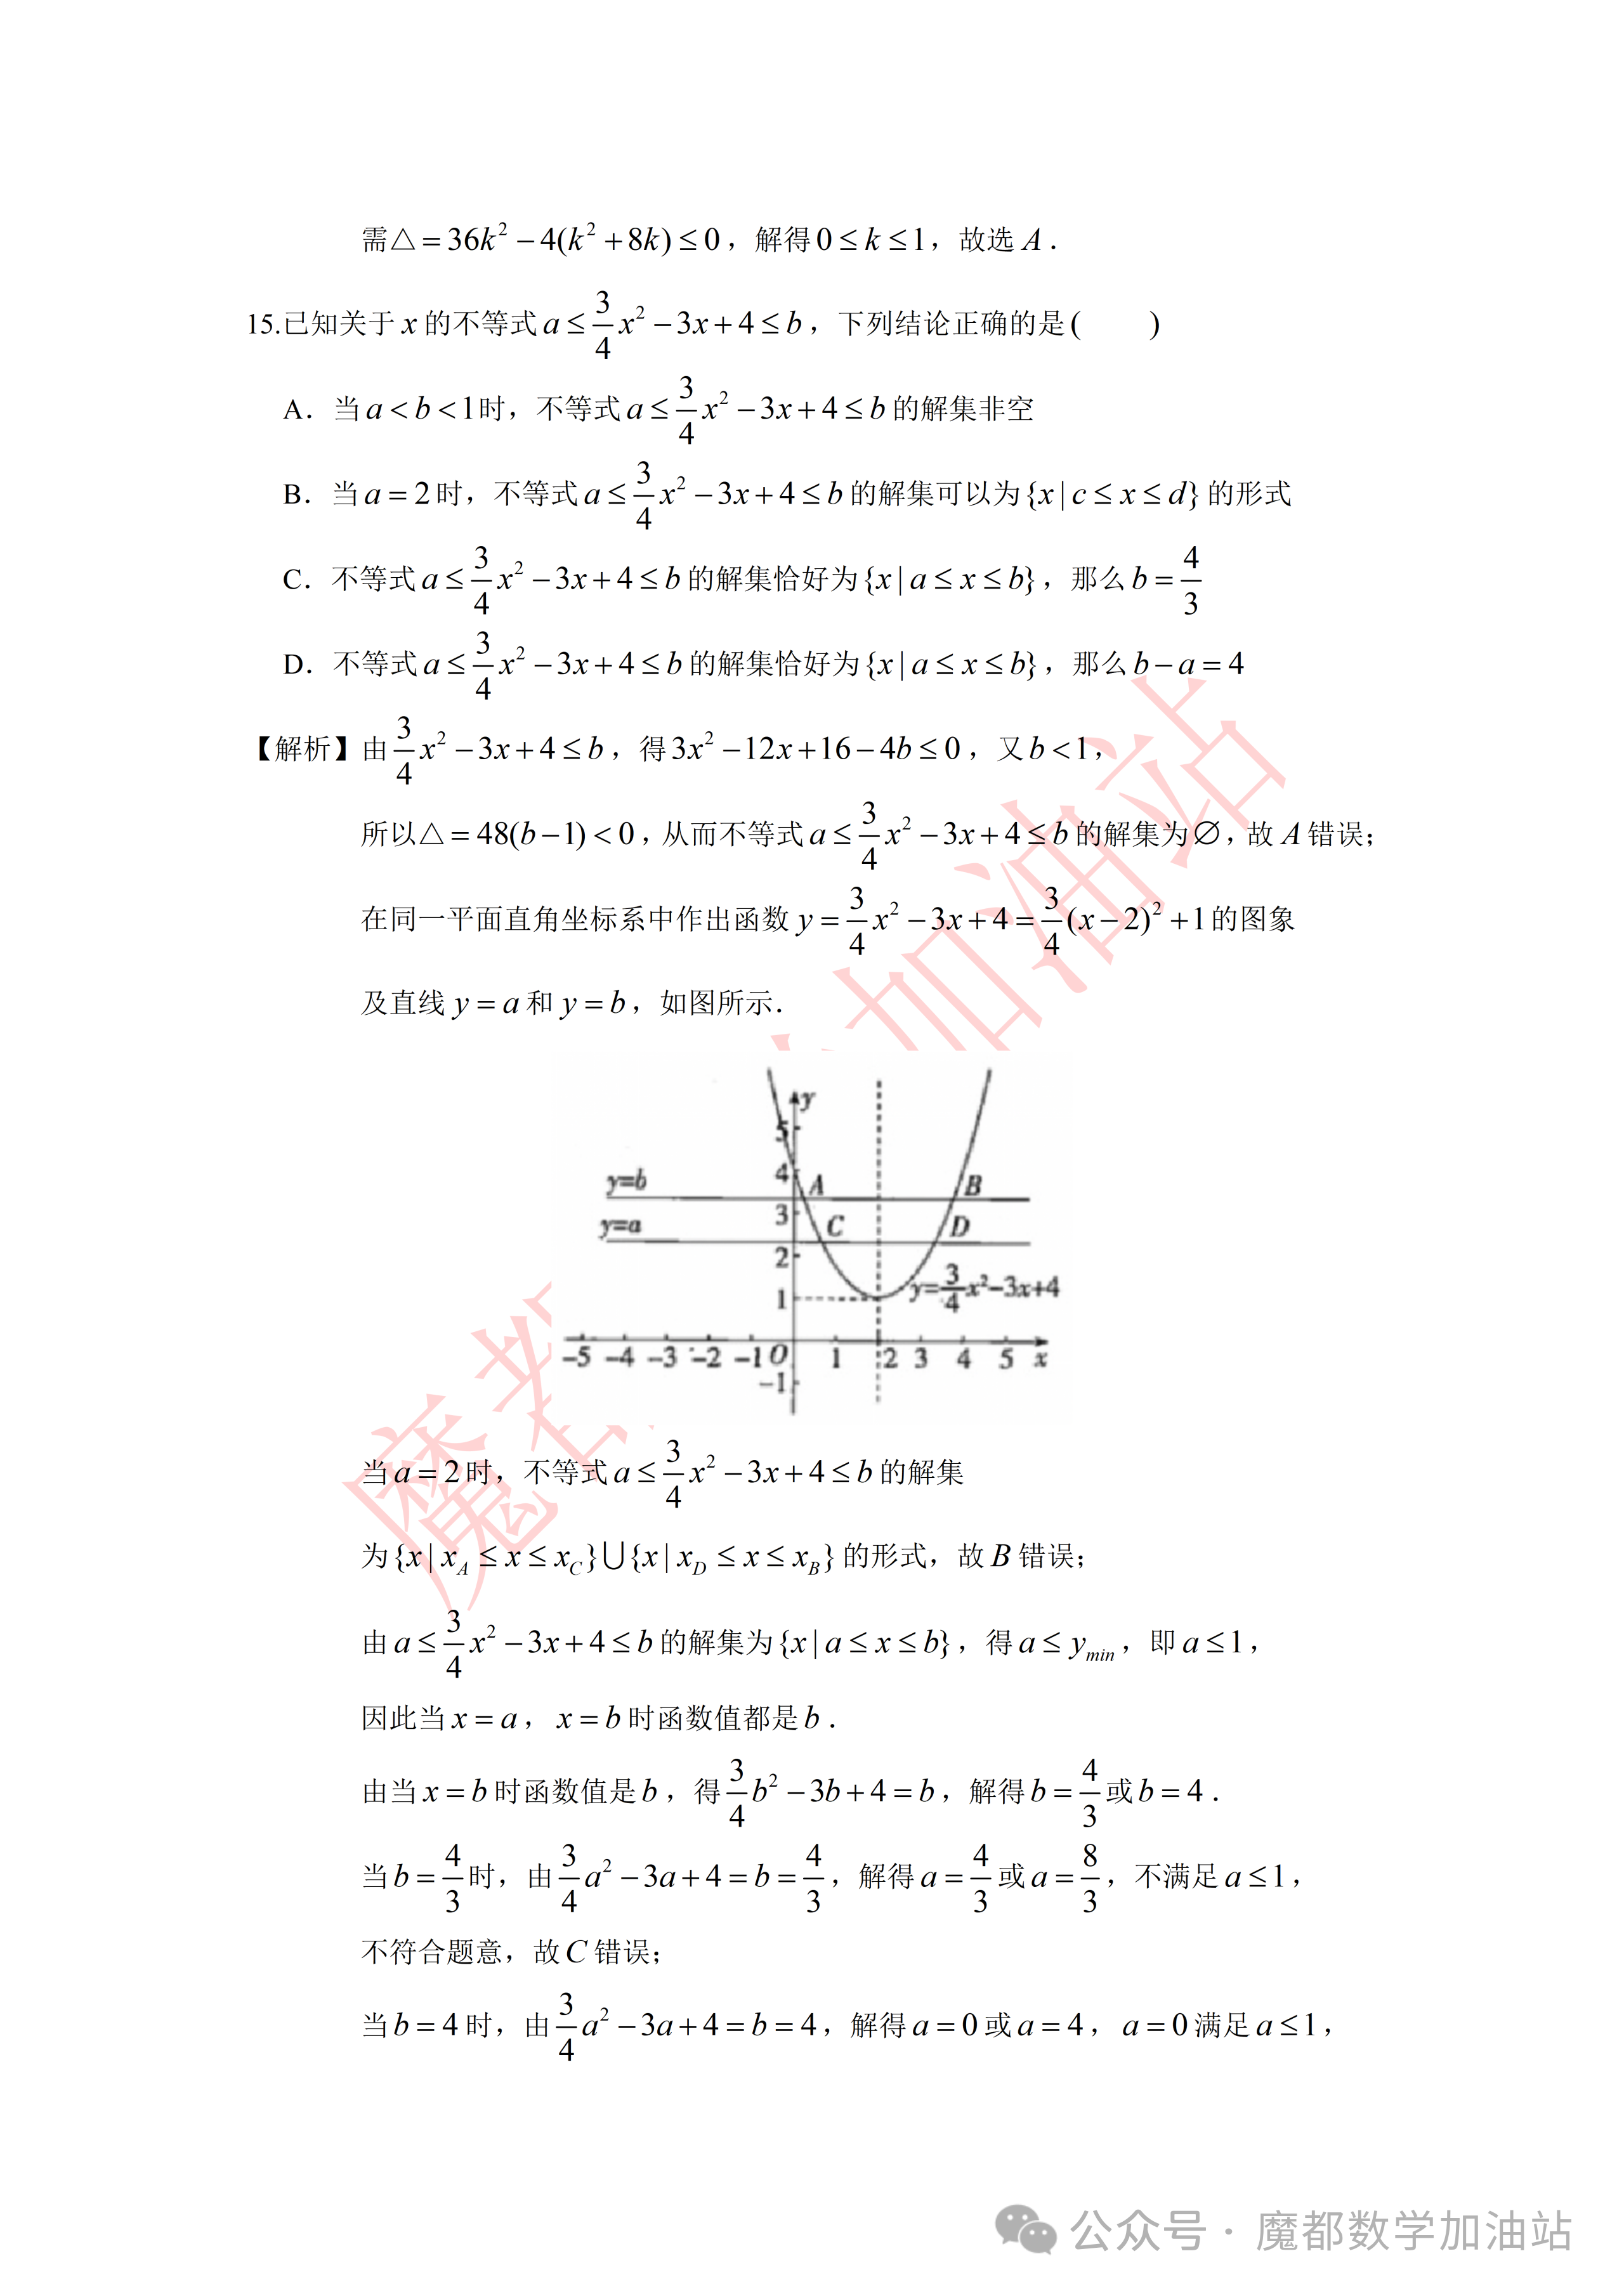
\includegraphics[width=.55\linewidth,trim=900bp 1400bp 760bp 1680bp,clip]{../原图/高一46_交附闵行_国庆作业3/05.png}
\end{center}
\step{当 $a=2$ 时，不等式 $a\leqslant\dfrac34x^2-3x+4\leqslant b$ 的解集为
$\{x\mid x_A\leqslant x\leqslant x_C\}\cup\{x\mid x_D\leqslant x\leqslant x_B\}$ 的形式，故 $B$ 错误；}
\step{由 $a\leqslant\dfrac34x^2-3x+4\leqslant b$ 的解集恰好为 $\{x\mid a\leqslant x\leqslant b\}$ 的形式，得 $a\leqslant y_{\min}$，即 $a\leqslant1$，}
\step{因为当 $x=a$、$x=b$ 时函数值都是 $b$，当 $x=a$ 时，$\dfrac34a^2-3a+4=b$；当 $x=b$ 时，$\dfrac34b^2-3b+4=b$，}
\step{解得 $b=\dfrac43$ 或 $b=4$，}
\step{当 $b=\dfrac43$ 时，由 $\dfrac34a^2-3a+4=b$，解得 $a=\dfrac43$ 或 $a=\dfrac83$，不符合题意，故 $C$ 错误；}
\step{当 $b=4$ 时，由 $\dfrac34a^2-3a+4=b$，解得 $a=0$ 或 $a=4$，$a=0$ 满足 $a\leqslant1$，故 $D$ 正确；}
\step{故选 $D$.}
\solend
\fi

\item 已知 $x$、$y\in(0,+\infty)$，则 $(x-y)^2+2y+1-x+\dfrac4x$ 的最小值为\mbox{（\quad）}

\keepwithprev
A. $1$\qquad B. $2$\qquad C. $3$\qquad D. $4$

\ans{$D$}

\ifanswer
\solbegin
\step{因为 $(x-y)^2+2y+1-x+\dfrac4x=(x-y-1)^2+x+\dfrac4x$，}
\step{当且仅当 $x-y-1=0$，且 $x=\dfrac4x$ 时取等号，}
\step{又因为 $x+\dfrac4x\geqslant2\sqrt{x\cdot\dfrac4x}=4$，当且仅当 $x=2$ 时取等号，}
\step{故选 $D$.}
\solend
\fi

\end{enumerate}

\bigsec{三、解答题}

\begin{enumerate}
\setcounter{enumi}{16}

\item 设集合 $A=\left\{x\middle|\dfrac{x-3}{x-1}<0\right\}$，$B=\{x\mid x^2-2ax+a^2-1>0\}$.
\begin{enumerate}[label=(\arabic*)]
\item 若 $a=3$，求 $A\cup B$；
\item 若“$x\in A$”是“$x\in B$”的充分条件，求实数 $a$ 的取值范围.
\end{enumerate}

\ifanswer
\solbegin
% 注：原卷题干为 a^2-1，故 a=3 时常数项为 8；题干与本步一致。
\stepm{(1)}{当 $a=3$ 时，$B=\{x\mid x^2-6x+8>0\}=\{x\mid x<2\text{ 或 }x>4\}$；}
\step{因为 $A=\left\{x\middle|\dfrac{x-3}{x-1}<0\right\}=\{x\mid(x-1)(x-3)<0\}=\{x\mid1<x<3\}$，}
\step{所以 $A\cup B=\{x\mid x<2\text{ 或 }x>4\}\cup\{x\mid1<x<3\}
=\{x\mid x<3\text{ 或 }x>4\}$.}
\stepm{(2)}{因为“$x\in A$”是“$x\in B$”的充分条件，所以 $A\subseteq B$，}
\step{因 $A=\left\{x\middle|\dfrac{x-3}{x-1}<0\right\}
=\{x\mid(x-1)(x-3)<0\}=\{x\mid1<x<3\}$，}
\step{所以 $A\subseteq B=\{x\mid x<a-1\text{ 或 }x>a+1\}$，}
\step{要使 $A\subseteq B$，需有 $a-1\geqslant3$ 或 $a+1\leqslant1$，}
\step{所以 $a\geqslant4$ 或 $a\leqslant0$，故 $a$ 的取值范围为 $\{a\mid a\geqslant4\text{ 或 }a\leqslant0\}$.}
\solend
\fi

\ansspace[6]

\item 某学校引入种植类劳动教育课程，打算围成如图所示的四块全等的长方形田地种植不同种类的蔬菜，其中一面可以利用原有的墙（足够长），其他各面需要用篱笆围成，设其中一块田地为矩形 $ABCD$.

\begin{center}
% 原图第 6 页配图直接裁取。
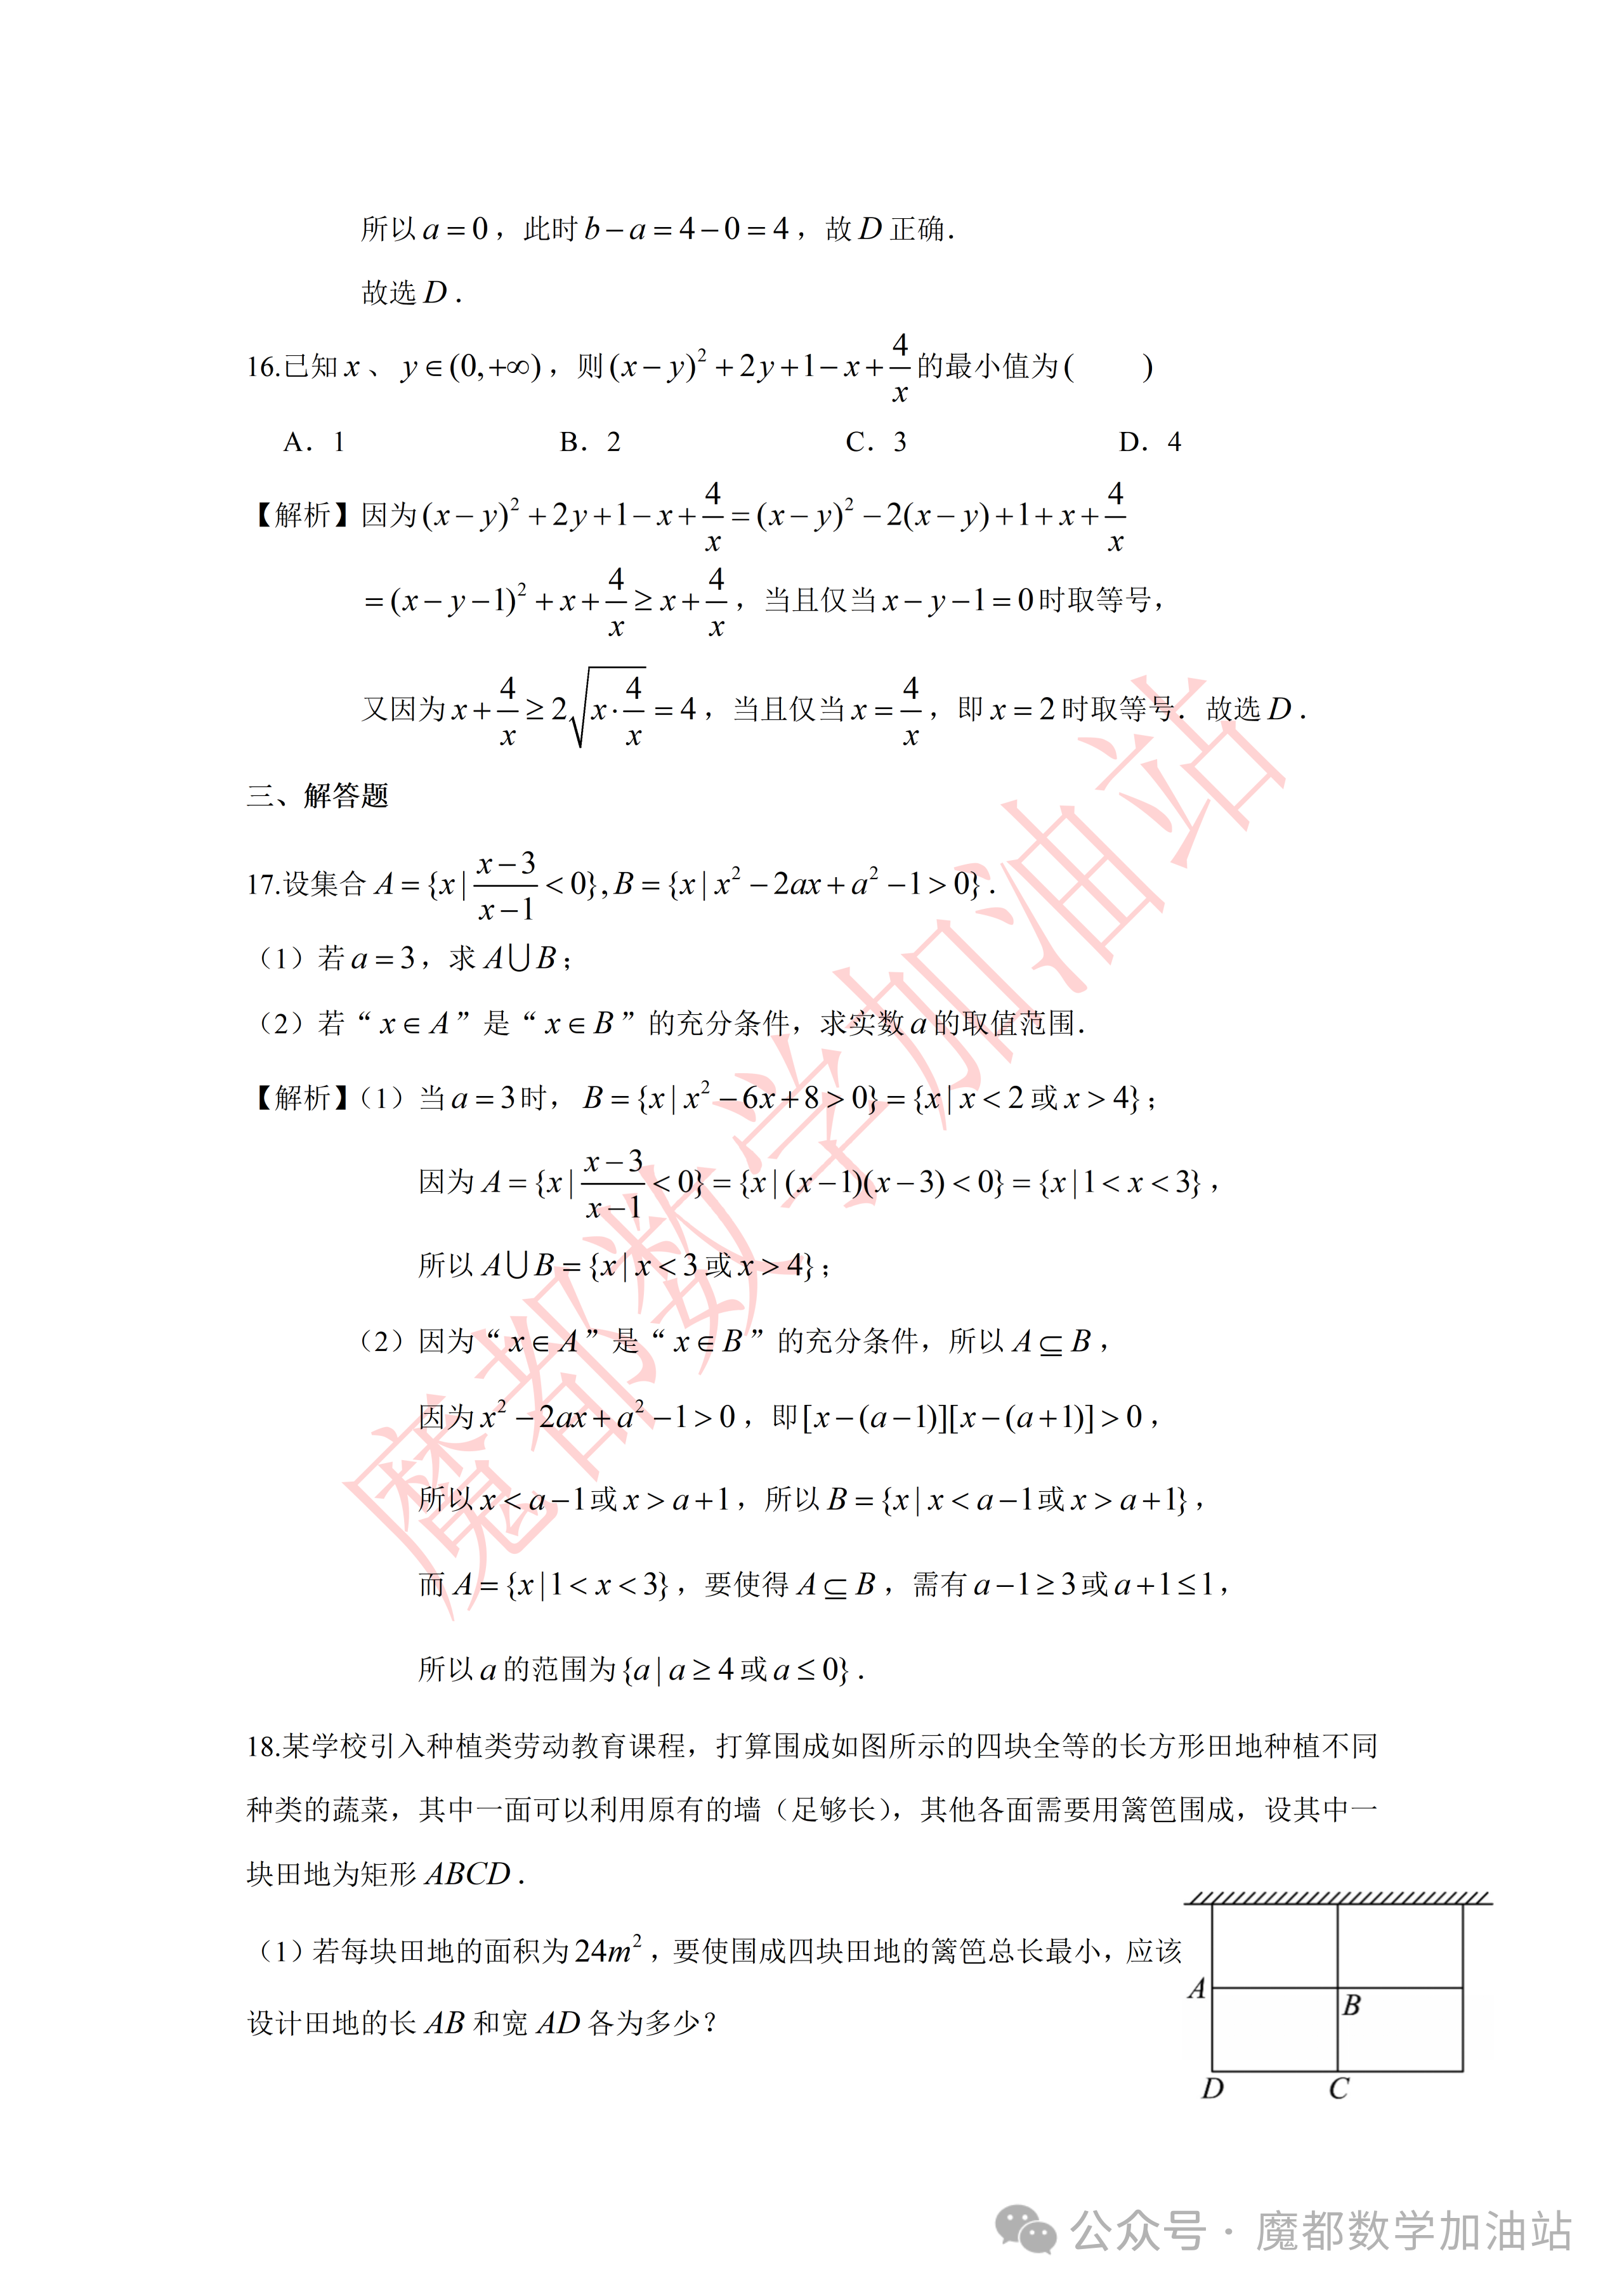
\includegraphics[width=.33\linewidth,trim=1866bp 220bp 210bp 2960bp,clip]{../原图/高一46_交附闵行_国庆作业3/06.png}
\end{center}

\begin{enumerate}[label=(\arabic*)]
\item 若每块田地的面积为 $24\,\text{m}^2$，要使围成四块田地的篱笆总长最小，应该设计田地的长 $AB$ 和宽 $AD$ 各为多少？
\item 现有 $40\,\text{m}$ 长的篱笆，要使每块田地的面积最大，应该设计田地的长 $AB$ 和宽 $AD$ 各为多少？
\end{enumerate}

\ifanswer
\solbegin
\stepm{(1)}{设 $AB$ 长为 $x\,\text{m}$，$AD$ 宽为 $y\,\text{m}$，由题意得 $xy=24$，篱笆总长为 $4x+6y$，}
\step{$4x+6y\geqslant2\sqrt{4x\cdot6y}=2\sqrt{24xy}=48$，}
\step{当且仅当 $4x=6y$ 时取等号，解得 $x=6$，$y=4$，}
\step{所以田地的长 $AB$ 为 $6\,\text{m}$，宽 $AD$ 为 $4\,\text{m}$.}
\stepm{(2)}{设 $AB$ 长为 $a\,\text{m}$，$AD$ 宽为 $b\,\text{m}$，由篱笆总长 $4a+6b=40$，即 $2a+3b=20$，}
\step{将 $a=\dfrac{20-3b}{2}$ 代入每块田地面积 $ab$，得 $ab=\dfrac12b(20-3b)=-\dfrac32b^2+10b$，}
\step{当 $b=\dfrac{10}{3}$ 时，$ab$ 最大，此时 $a=5$，}
\step{所以田地的长 $AB$ 为 $5\,\text{m}$，宽 $AD$ 为 $\dfrac{10}{3}\,\text{m}$.}
\solend
\fi

\ansspace[8]

\item 已知 $x_1$、$x_2$ 是一元二次方程 $4kx^2-4kx+k+1=0$ 的两个不等实数根.
\begin{enumerate}[label=(\arabic*)]
\item 若 $x_1$、$x_2$ 均为正根，求实数 $k$ 的取值范围；
\item 求使 $\dfrac{x_1}{x_2}+\dfrac{x_2}{x_1}-2$ 的值为整数 $k$ 的整数值.
\end{enumerate}

\ifanswer
\solbegin
\stepm{(1)}{由题意，$x_1$、$x_2$ 是方程 $4kx^2-4kx+k+1=0$ 的两个不等实数根，}
\step{故 $k\neq0$，$\Delta=(-4k)^2-16k(k+1)>0$，得 $-16k>0$，所以 $k<0$，}
\step{又 $x_1+x_2=1$，$x_1x_2=\dfrac{k+1}{4k}>0$，得 $k+1<0$，}
\step{所以 $k$ 的取值范围为 $(-\infty,-1)$.}
\stepm{(2)}{由题意，}
\step{$\dfrac{x_1}{x_2}+\dfrac{x_2}{x_1}-2
=\dfrac{x_1^2+x_2^2-2x_1x_2}{x_1x_2}
=\dfrac{(x_1+x_2)^2-4x_1x_2}{x_1x_2}$，}
\step{又 $x_1+x_2=1$，$x_1x_2=\dfrac{k+1}{4k}$，}
\step{则 $\dfrac{x_1}{x_2}+\dfrac{x_2}{x_1}-2=-\dfrac4{k+1}$，}
\step{由于 $-\dfrac4{k+1}$ 为整数，故 $k+1$ 只能取 $\pm1$、$\pm2$、$\pm4$，又 $k<-1$，}
\step{所以整数 $k$ 的值为 $-2$、$-3$、$-5$.}
\solend
\fi

\ansspace[8]

\item 已知 $a>0$，$b>0$，且 $2a+3b=3$.
\begin{enumerate}[label=(\arabic*)]
\item 求 $ab$ 的最大值；
\item 求 $a-\dfrac1{6b}$ 的最大值；
\item 求 $\dfrac2a+\dfrac3{b+1}$ 的最小值.
\end{enumerate}

\ifanswer
\solbegin
\stepm{(1)}{由 $2a+3b=3$，得 $3=2a+3b\geqslant2\sqrt{6ab}$，}
\step{所以 $ab\leqslant\dfrac38$，当且仅当 $2a=3b=\dfrac32$ 时取等号，}
\step{故 $ab$ 的最大值为 $\dfrac38$.}
\stepm{(2)}{由 $2a+3b=3$，得 $a=\dfrac32-\dfrac32b$，}
\step{则 $a-\dfrac1{6b}=\dfrac32-\dfrac32b-\dfrac1{6b}$，}
\step{由基本不等式，$\dfrac32b+\dfrac1{6b}\geqslant2\sqrt{\dfrac32b\cdot\dfrac1{6b}}=1$，}
\step{当且仅当 $\dfrac32b=\dfrac1{6b}$，即 $b=\dfrac13$、$a=1$ 时取等号，}
\step{所以 $a-\dfrac1{6b}$ 的最大值为 $\dfrac12$.}
\stepm{(3)}{由 $2a+3b=3$，得 $2a+3(b+1)=6$，}
\step{$\dfrac2a+\dfrac3{b+1}
=\dfrac16\left(2a+3(b+1)\right)\left(\dfrac2a+\dfrac3{b+1}\right)$}
\step{$=\dfrac16\left(13+\dfrac{6(b+1)}a+\dfrac{6a}{b+1}\right)
\geqslant\dfrac16\left(13+2\sqrt{\dfrac{6(b+1)}a\cdot\dfrac{6a}{b+1}}\right)=\dfrac{25}{6}$，}
\step{当且仅当 $a=b+1$，即 $a=\dfrac65$、$b=\dfrac15$ 时取等号，}
\step{所以 $\dfrac2a+\dfrac3{b+1}$ 的最小值为 $\dfrac{25}{6}$.}
\solend
\fi

\ansspace[8]

\item 已知 $U=\R$ 为全集，集合 $A=\{s^2+3t^2\mid s,t\in U\}$.
\begin{enumerate}[label=(\arabic*)]
\item 设 $U=\{1,3,5\}$，求集合 $A$ 的元素个数；
\item 设 $U=\Z$，证明：若 $x\in A$，则 $7x\in A$；
\item 设 $U=\R$，$x$、$y\in A$，且 $x=m^2+3n^2$，$y=p^2+3q^2$，若 $mp-3nq=\sqrt3$，求 $x+y+mq+np$ 的最小值.
\end{enumerate}

\ifanswer
\solbegin
\stepm{(1)}{当 $s=1$，$t=1$ 时，$s^2+3t^2=1+3=4$；}
\step{当 $s=1$，$t=3$ 时，$s^2+3t^2=1+27=28$；}
\step{当 $s=1$，$t=5$ 时，$s^2+3t^2=1+75=76$；}
\step{当 $s=3$，$t=1$ 时，$s^2+3t^2=9+3=12$；}
\step{当 $s=3$，$t=3$ 时，$s^2+3t^2=9+27=36$；}
\step{当 $s=3$，$t=5$ 时，$s^2+3t^2=9+75=84$；}
\step{当 $s=5$，$t=1$ 时，$s^2+3t^2=25+3=28$；}
\step{当 $s=5$，$t=3$ 时，$s^2+3t^2=25+27=52$；}
\step{当 $s=5$，$t=5$ 时，$s^2+3t^2=25+75=100$，}
\step{所以 $A=\{4,12,28,36,52,76,84,100\}$，有 $8$ 个元素.}
\stepm{(2)}{因为 $U=\Z$，$x\in A$，设 $x=s^2+3t^2$，}
\step{则 $7x=7(s^2+3t^2)=(2s+3t)^2+3(s-2t)^2\in A$，}
\step{所以 $7x\in A$.}
\stepm{(3)}{因为 $x=m^2+3n^2$，$y=p^2+3q^2$，}
\step{$xy=(m^2+3n^2)(p^2+3q^2)=3(mq+np)^2+(mp-3nq)^2$，}
\step{设 $mq+np=b$，则 $xy=3b^2+3$，所以 $y=\dfrac{3b^2+3}{x}$，}
\step{于是 $x+y+mq+np=x+\dfrac{3b^2+3}{x}+b\geqslant2\sqrt{3b^2+3}+b$，}
\step{设 $2\sqrt{3b^2+3}+b=t$，整理得 $11b^2+2bt+12-t^2=0$，}
\step{判别式法，$\Delta=4t^2-44(12-t^2)\geqslant0$，得 $t\geqslant\sqrt{11}$，}
\step{即 $(x+y+mq+np)_{\min}=\sqrt{11}$，所以 $x+y+mq+np$ 的最小值为 $\sqrt{11}$.}
\solend
\fi

\ansspace*[10]

\end{enumerate}

\end{document}
"
%
% 原始材料：微信公众号“魔都数学加油站”，作者破晓，2026-10-02 17:56 发布。
% 原文标题：“27学年高一46——2026-2027你那上海市交附闵行高一上国庆作业3”
% （公众号标题中的“你那”照录，系原文标题字样）；原文链接：
% http://mp.weixin.qq.com/s?__biz=Mzg4ODU1ODMxOQ==&mid=2247591657&idx=3&sn=a894d1a16611283a61b3eaba32a3f24c&chksm=cee83366c6a55381b370069f84ef63d20251f94608bb37cc4ec2d66227401bd147f4f6bd8256&scene=126&sessionid=1790935402&subscene=7&clicktime=1790937618&enterid=1790937618#rd
% 正文为 9 张 PNG 页，按页序读取原图；第 01、02、07 页 4762×6735，
% 第 03—06、08、09 页 2560×3620。卷面标题照原卷印作“2026-2027 年交附闵行高一上国庆作业 3”。
% 原文从第 3 题起，题号照原卷保留；正文为讲评版，答案、解析依原卷顺序录入。
% 水印及页脚公众号标识不录入。卷面插图直接裁取对应原图页，不另制图片文件。
%
% 与原卷的排版差异：
%   ① 原卷按“一、填空题”“二、选择题”“三、解答题”分节，本稿沿用原节与原题号，
%      只改排为全稿统一的大节样式；
%   ② 原卷答案与解析依页面位置分布，本稿按 common.sty 统一置于答案版；
%   ③ 原卷副标题未印，本稿按“知识模块”口径标作“集合与常用逻辑用语、不等式”。
%
% 原卷存疑一处（照抄未改，见第 12 题题干及解析处注释）：
%   第 12 题题干同时给出 x∈Z，却称不等式组有“50 个不等的实数解”；解析按整数根计数。
%   此处题干与解析的原文不一致，本稿均照录。
% 第 17 题曾疑似有常数项不一致：复核原图题干为 a^2-1，a=3 时常数项确为 8，
% 与解析相符；不将其记作原卷错误。
%
\documentclass[a4paper,11pt]{article}
\usepackage{common}

\begin{document}

\examtitlest[3]{2026--2027 年交附闵行高一上国庆作业 3}{集合与常用逻辑用语、不等式}

\bigsec{一、填空题}

\begin{enumerate}
\setcounter{enumi}{2}

\item 不等式 $\dfrac{x^2-10}{x+2}\geqslant1$ 的解集为\blankline[4.4em].

\ifanswer
\ans{$\{x\mid-3\leqslant x<-2\text{ 或 }x\geqslant4\}$}
\solbegin
\step{不等式 $\dfrac{x^2-10}{x+2}\geqslant1$，移项得 $\dfrac{x^2-10}{x+2}-1\geqslant0$，}
\step{通分得 $\dfrac{x^2-x-12}{x+2}\geqslant0$，即 $\dfrac{(x-4)(x+3)}{x+2}\geqslant0$，}
\step{解得 $-3\leqslant x<-2$ 或 $x\geqslant4$，}
\step{故不等式的解集为 $\{x\mid-3\leqslant x<-2\text{ 或 }x\geqslant4\}$.}
\solend
\fi

\item $|x-3|+|x-5|\geqslant2$，当等号成立时，$x$ 的范围是\blankline[4.4em].

\ifanswer
\ans{$[3,5]$}
\fi

\item 若直角三角形斜边长等于 $4\sqrt2\,\text{cm}$，则直角三角形面积的最大值为\blankline[4.4em].

\ifanswer
\solbegin
\step{设 $Rt\triangle ABC$ 中，$C=90^\circ$，则 $c=\sqrt{a^2+b^2}=4\sqrt2$，所以 $a^2+b^2=32$，}
\step{由基本不等式得 $a^2+b^2\geqslant2ab$，当且仅当 $a=b=4$ 时取等号，}
\step{所以 $\triangle ABC$ 的面积 $S=\dfrac12ab\leqslant8$，}
\step{当且仅当 $a=b=4$ 时，$\triangle ABC$ 的面积最大值为 $8$.}
\solend
\fi

\item 不等式 $(x-1)(2-x)>0$ 的解集为\blankline[4.4em].

\ifanswer
\solbegin
\step{$(x-1)(2-x)>0\Rightarrow(x-1)(x-2)<0$，}
\step{故不等式的解集为 $\{x\mid1<x<2\}$.}
\solend
\fi

\item 已知集合 $A=\{1,2\}$，$B=\{x\mid x^2-2mx+m=0\}$，$A\cup B=A$，则实数 $m$ 的取值范围为\blankline[4.4em].

\ifanswer
\solbegin
\step{因为 $A\cup B=A$，所以 $B\subseteq A$，}
\step{当 $B=\varnothing$ 时，$\Delta=(-2m)^2-4m<0$，解得 $0<m<1$，}
\step{当 $B$ 为单元素集时，$\Delta=0$，解得 $m=0$ 或 $m=1$，}
\step{当 $m=0$ 时，方程 $x^2=0$，解得 $x=0$，此时 $B=\{0\}$，不满足 $B\subseteq A$；}
\step{当 $m=1$ 时，方程 $x^2-2x+1=0$，解得 $x=1$，此时 $B=\{1\}$，满足 $B\subseteq A$；}
\step{当 $B=\{1,2\}$ 时，由韦达定理得 $1+2=2m$，$1\times2=m$，无解，}
\step{综上所述，实数 $m$ 的取值范围为 $\{m\mid0<m\leqslant1\}$.}
\solend
\fi

\item 设 $a$、$b$、$c\in\R^+$，若 $a+b+c=1$，则 $\dfrac1a+\dfrac1b+\dfrac1c\geqslant$\blankline[4.4em].

\ifanswer
\solbegin
\step{因为 $a$、$b$、$c\in\R^+$，且 $a+b+c=1$，}
\step{所以 $\dfrac1a+\dfrac1b+\dfrac1c=(a+b+c)\left(\dfrac1a+\dfrac1b+\dfrac1c\right)$}
\step{$=3+\dfrac ab+\dfrac ba+\dfrac ac+\dfrac ca+\dfrac bc+\dfrac cb$，}
\step{由基本不等式得 $\dfrac ab+\dfrac ba\geqslant2$，$\dfrac ac+\dfrac ca\geqslant2$，$\dfrac bc+\dfrac cb\geqslant2$，}
\step{所以 $\dfrac1a+\dfrac1b+\dfrac1c\geqslant9$，当且仅当 $a=b=c=\dfrac13$ 时取等号，}
\step{所以 $\dfrac1a+\dfrac1b+\dfrac1c$ 的最小值为 $9$.}
\solend
\fi

\item 已知 $-1\leqslant x+y\leqslant2$，$-2\leqslant x-y\leqslant1$，则 $x-2y$ 的范围为\blankline[4.4em].

\ifanswer
\solbegin
\step{设 $x-2y=m(x+y)+n(x-y)$，}
\step{则 $x-2y=(m+n)x+(m-n)y$，所以 $m+n=1$，$m-n=-2$，}
\step{解得 $m=-\dfrac12$，$n=\dfrac32$，}
\step{所以 $x-2y=-\dfrac12(x+y)+\dfrac32(x-y)$，}
\step{因为 $-1\leqslant x+y\leqslant2$，$-2\leqslant x-y\leqslant1$，}
\step{所以 $-4\leqslant x-2y\leqslant2$，即 $x-2y$ 的范围为 $[-4,2]$.}
\solend
\fi

\item 设集合 $A=\{1,2,m\}$，其中 $m$ 为实数，令 $B=\{a^2\mid a\in A\}$，$C=A\cup B$. 若 $C$ 中所有元素之和为 $6$，则 $C$ 中的所有元素之积为\blankline[4.4em].

\ifanswer
\solbegin
\step{因为 $A=\{1,2,m\}$，所以 $B=\{a^2\mid a\in A\}=\{1,4,m^2\}$，$m\neq1$，$m\neq2$，}
\step{又 $C=A\cup B$，所以 $1\in C$，$4\in C$，$m^2\in C$，}
\step{若 $m^2=1$，则 $m=-1$ 或 $m=1$（舍），当 $m=-1$ 时，$C=\{1,2,4,-1\}$，$C$ 中所有元素之和为 $6$，}
\step{此时 $C$ 中所有元素之积为 $-8$；}
\step{若 $m^2=2$，则 $m=-\sqrt2$ 或 $m=\sqrt2$，$C$ 中所有元素之和不符合题意；}
\step{若 $m^2=4$，则 $m=-2$ 或 $m=2$，此时 $C=\{1,2,4,-2\}$ 或 $C=\{1,2,4\}$，所有元素之和不符合题意；}
\step{若 $m^2\neq1$，$m^2\neq2$，$m^2\neq4$，则 $C=\{1,2,4,m,m^2\}$，}
\step{所以 $1+2+4+m+m^2=6$，即 $m^2+m+1=0$，无解，}
\step{综上所述，$C$ 中所有元素之积为 $-8$.}
\solend
\fi

\item 若对任意实数 $x>0$，$y>0$，不等式 $x+\sqrt{xy}\leqslant a(x+y)$ 恒成立，则实数 $a$ 的最小值为\blankline[4.4em].

\ifanswer
\solbegin
\step{由不等式 $x+\sqrt{xy}\leqslant a(x+y)$ 对任意实数 $x>0$，$y>0$ 恒成立，}
\step{得 $a\geqslant\dfrac{x+\sqrt{xy}}{x+y}$，}
\step{设 $\sqrt{\dfrac yx}=t>0$，则 $a\geqslant\dfrac{1+t}{1+t^2}$，}
\step{$\dfrac{1+t}{1+t^2}\leqslant\dfrac{\sqrt2+1}{2}$，当且仅当 $t=\sqrt2-1$ 时取等号，}
\step{所以实数 $a$ 的最小值为 $\dfrac{\sqrt2+1}{2}$.}
\solend
\fi

% 注：原卷题干给出 x∈Z，却写“实数解”；解析按整数解计数，题干与解析不一致，照录未改。
\item 若关于 $x$ 的不等式组
$\begin{cases}x^2-3mx\geqslant4m^2\\-20<x<120\end{cases}$（$x\in\Z,m>0$）恰有 $50$ 个不等的实数解，则 $m$ 的取值范围为\blankline[4.4em]（结果用区间表示）.

\ifanswer
\solbegin
\step{由 $x^2-3mx\geqslant4m^2$ 以及 $m>0$，解得 $x\leqslant-m$ 或 $x\geqslant4m$，}
\step{由原不等式组恰有 $50$ 个不等的实数解，可画出如下解集区间：}
\begin{center}
% 原图第 4 页数轴图直接裁取。
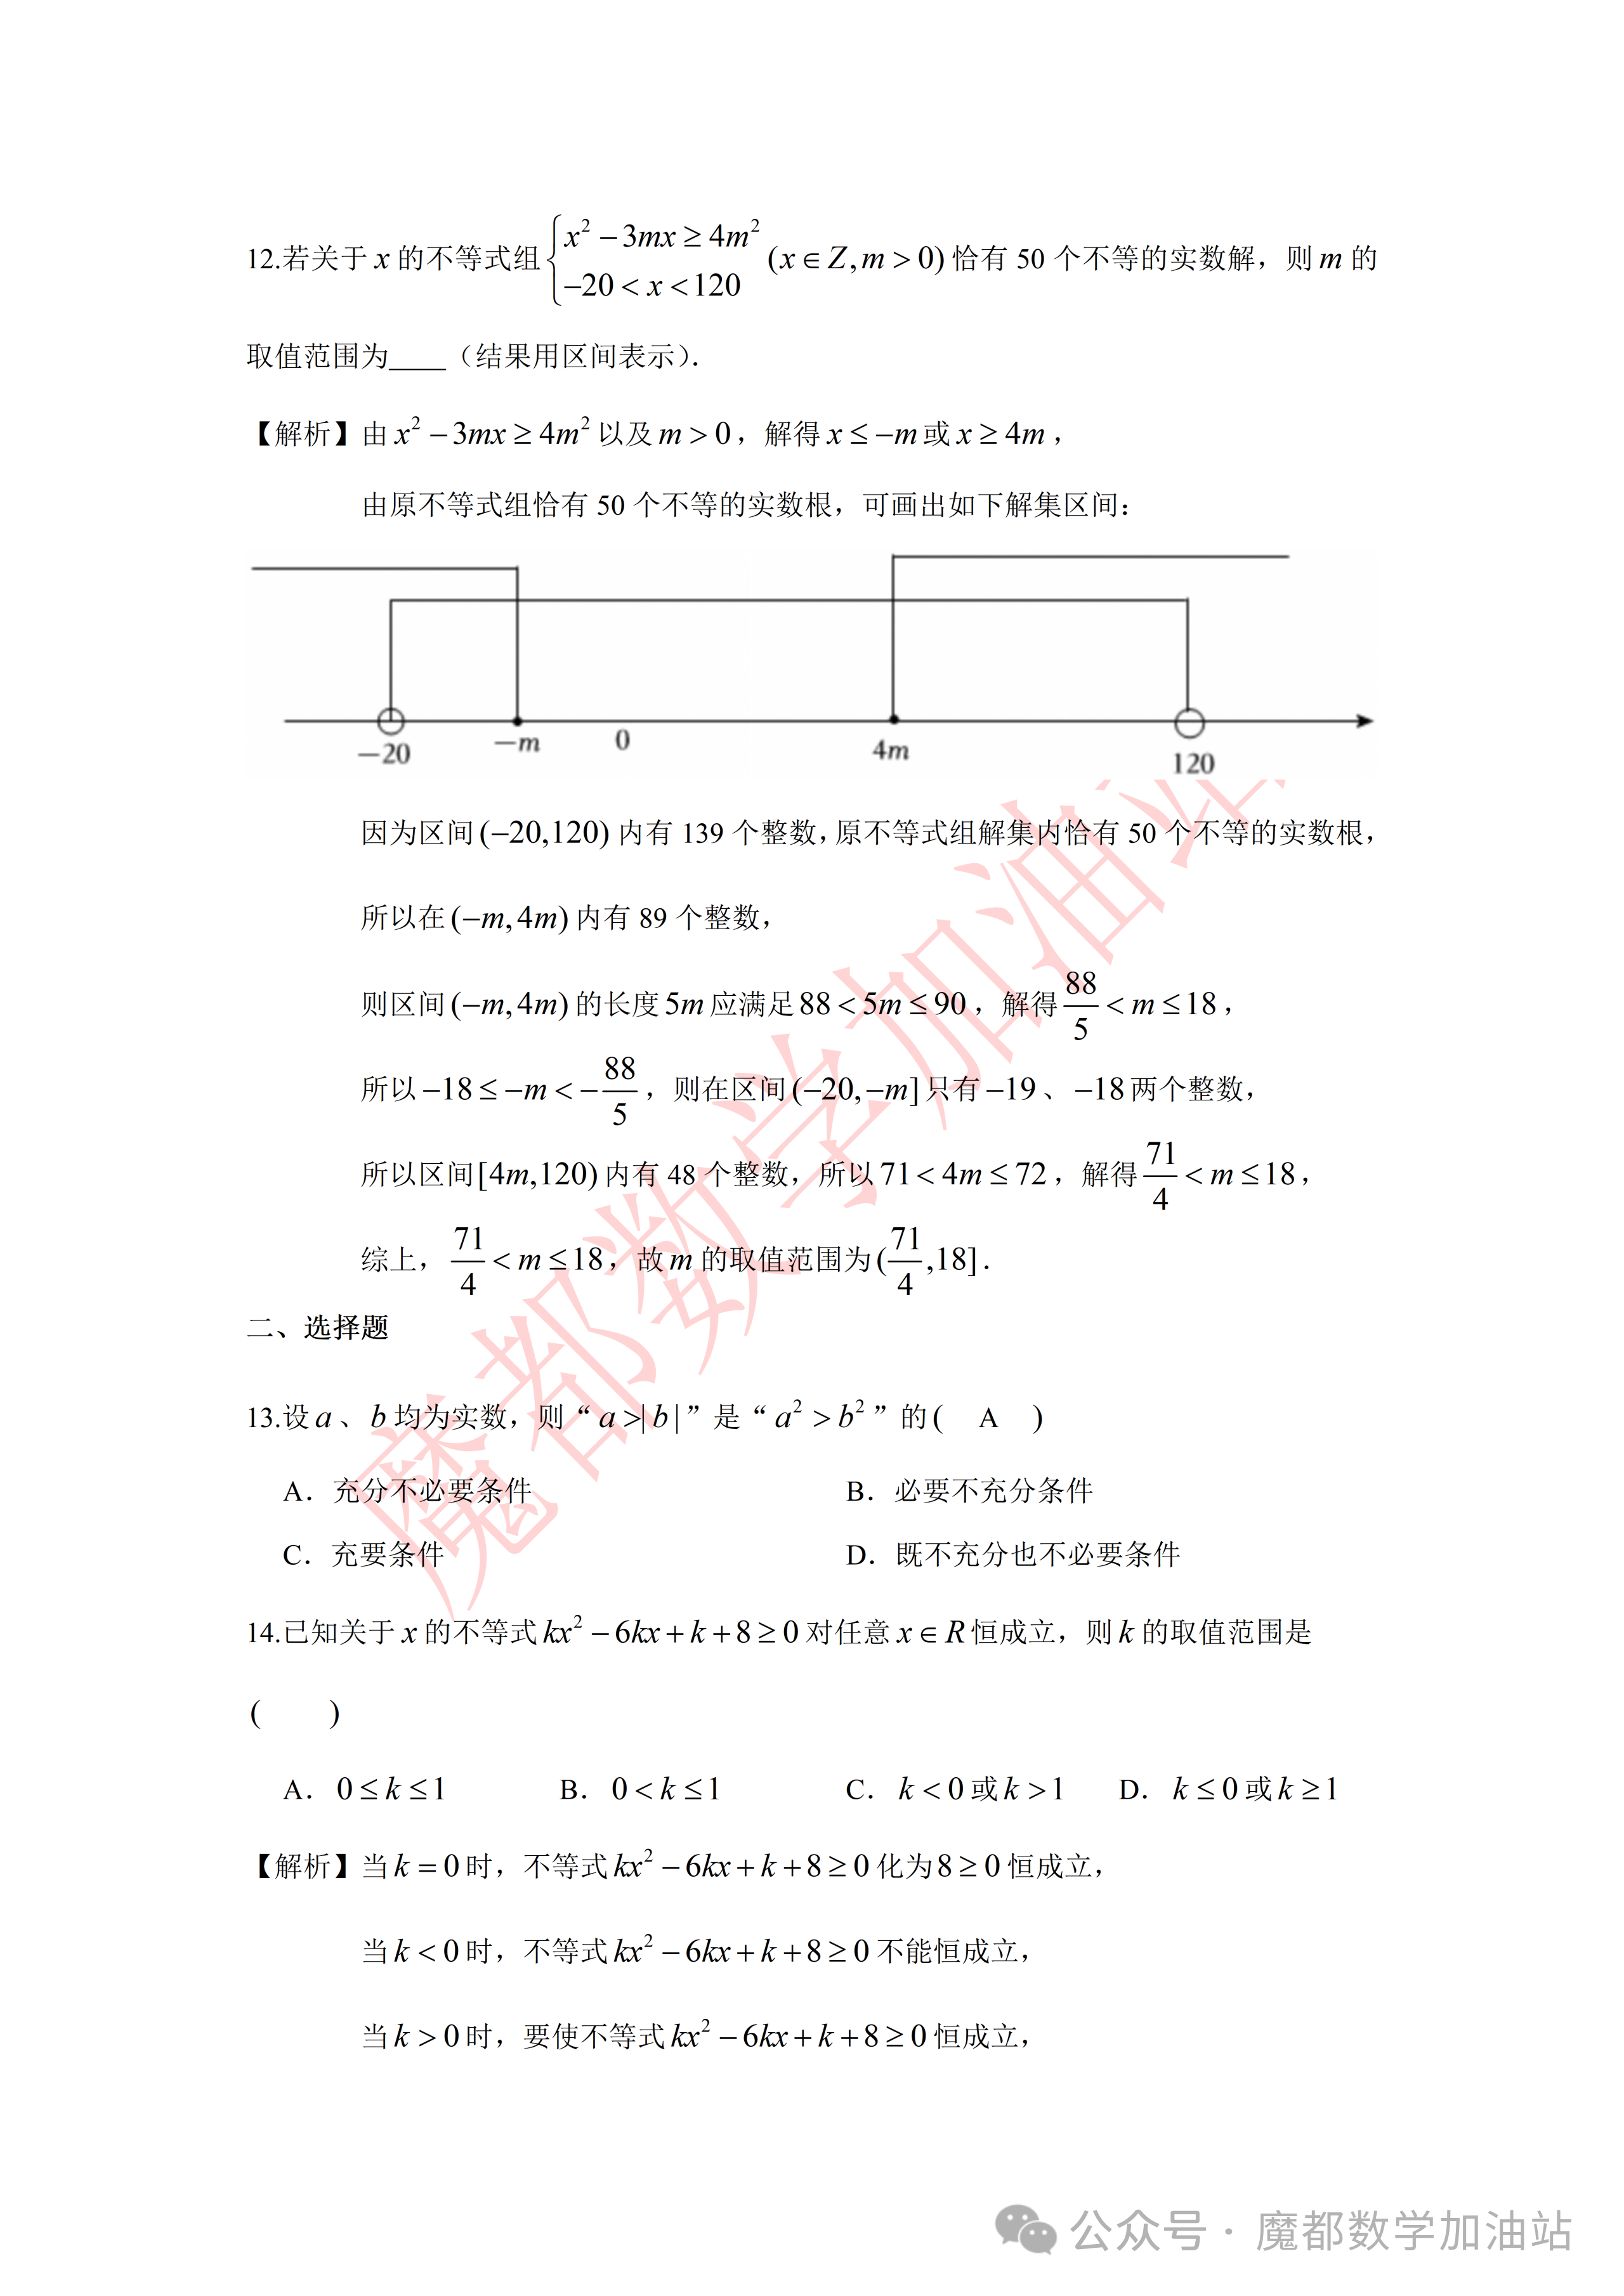
\includegraphics[width=.88\linewidth,trim=400bp 2410bp 320bp 860bp,clip]{../原图/高一46_交附闵行_国庆作业3/04.png}
\end{center}
\step{因为区间 $(-20,120)$ 内有 $139$ 个整数，原不等式组解集内有 $50$ 个不等的整数根，}
\step{所以在区间 $(-m,4m)$ 内有 $89$ 个整数，}
\step{则区间 $(-m,4m)$ 的长度 $5m$ 应满足 $88<5m\leqslant90$，解得 $\dfrac{88}{5}<m\leqslant18$，}
% 注：原卷题干称“实数解”，本行及后文按原卷解析照录为整数根计数。
\step{所以 $-18\leqslant-m<-\dfrac{88}{5}$，则在区间 $(-20,-m]$ 内有 $-19$、$-18$ 两个整数，}
\step{所以区间 $[4m,120)$ 内有 $48$ 个整数，}
\step{则 $71<4m\leqslant72$，解得 $\dfrac{71}{4}<m\leqslant18$，}
\step{综上，$\dfrac{71}{4}<m\leqslant18$，故 $m$ 的取值范围为 $\left(\dfrac{71}{4},18\right]$.}
\solend
\fi

\end{enumerate}

\bigsec{二、选择题}

\begin{enumerate}
\setcounter{enumi}{12}

\item 设 $a$、$b$ 均为实数，则“$a>|b|$”是“$a^2>b^2$”的\mbox{（\quad）}

\keepwithprev
A. 充分不必要条件\qquad B. 必要不充分条件

C. 充要条件\qquad\qquad D. 既不充分也不必要条件

\ans{$A$}

\item 已知关于 $x$ 的不等式 $kx^2-6kx+k+8\geqslant0$ 对任意 $x\in\R$ 恒成立，则 $k$ 的取值范围是\mbox{（\quad）}

\keepwithprev
A. $0\leqslant k\leqslant1$\qquad B. $0<k\leqslant1$

C. $k<0$ 或 $k>1$\qquad D. $k\leqslant0$ 或 $k\geqslant1$

\ans{$A$}

\ifanswer
\solbegin
\step{当 $k=0$ 时，不等式 $kx^2-6kx+k+8\geqslant0$ 化为 $8\geqslant0$ 恒成立，}
\step{当 $k<0$ 时，不等式 $kx^2-6kx+k+8\geqslant0$ 不能恒成立，}
\step{当 $k>0$ 时，要使不等式 $kx^2-6kx+k+8\geqslant0$ 恒成立，}
\step{需 $\Delta=36k^2-4(k^2+8k)\leqslant0$，解得 $0\leqslant k\leqslant1$，故选 $A$.}
\solend
\fi

\item 已知关于 $x$ 的不等式 $a\leqslant\dfrac34x^2-3x+4\leqslant b$，下列结论正确的是\mbox{（\quad）}

\keepwithprev
A. 当 $a<b<1$ 时，不等式 $a\leqslant\dfrac34x^2-3x+4\leqslant b$ 的解集非空

B. 当 $a=2$ 时，不等式 $a\leqslant\dfrac34x^2-3x+4\leqslant b$ 的解集可以为 $\{x\mid c\leqslant x\leqslant d\}$ 的形式

C. 不等式 $a\leqslant\dfrac34x^2-3x+4\leqslant b$ 的解集恰好为 $\{x\mid a\leqslant x\leqslant b\}$，那么 $b=\dfrac43$

D. 不等式 $a\leqslant\dfrac34x^2-3x+4\leqslant b$ 的解集恰好为 $\{x\mid a\leqslant x\leqslant b\}$，那么 $b-a=4$

\ans{$D$}

\ifanswer
\solbegin
\step{由 $\dfrac34x^2-3x+4\leqslant b$，得 $3x^2-12x+16-4b\leqslant0$，又 $b<1$，}
\step{所以 $\Delta=144-12(16-4b)=48(b-1)<0$，从而不等式无解，故 $A$ 错误；}
\step{在同一平面直角坐标系中作出函数 $y=\dfrac34x^2-3x+4=\dfrac34(x-2)^2+1$ 的图象及直线 $y=a$ 和 $y=b$，如图所示.}
\begin{center}
% 原图第 5 页解析配图直接裁取。
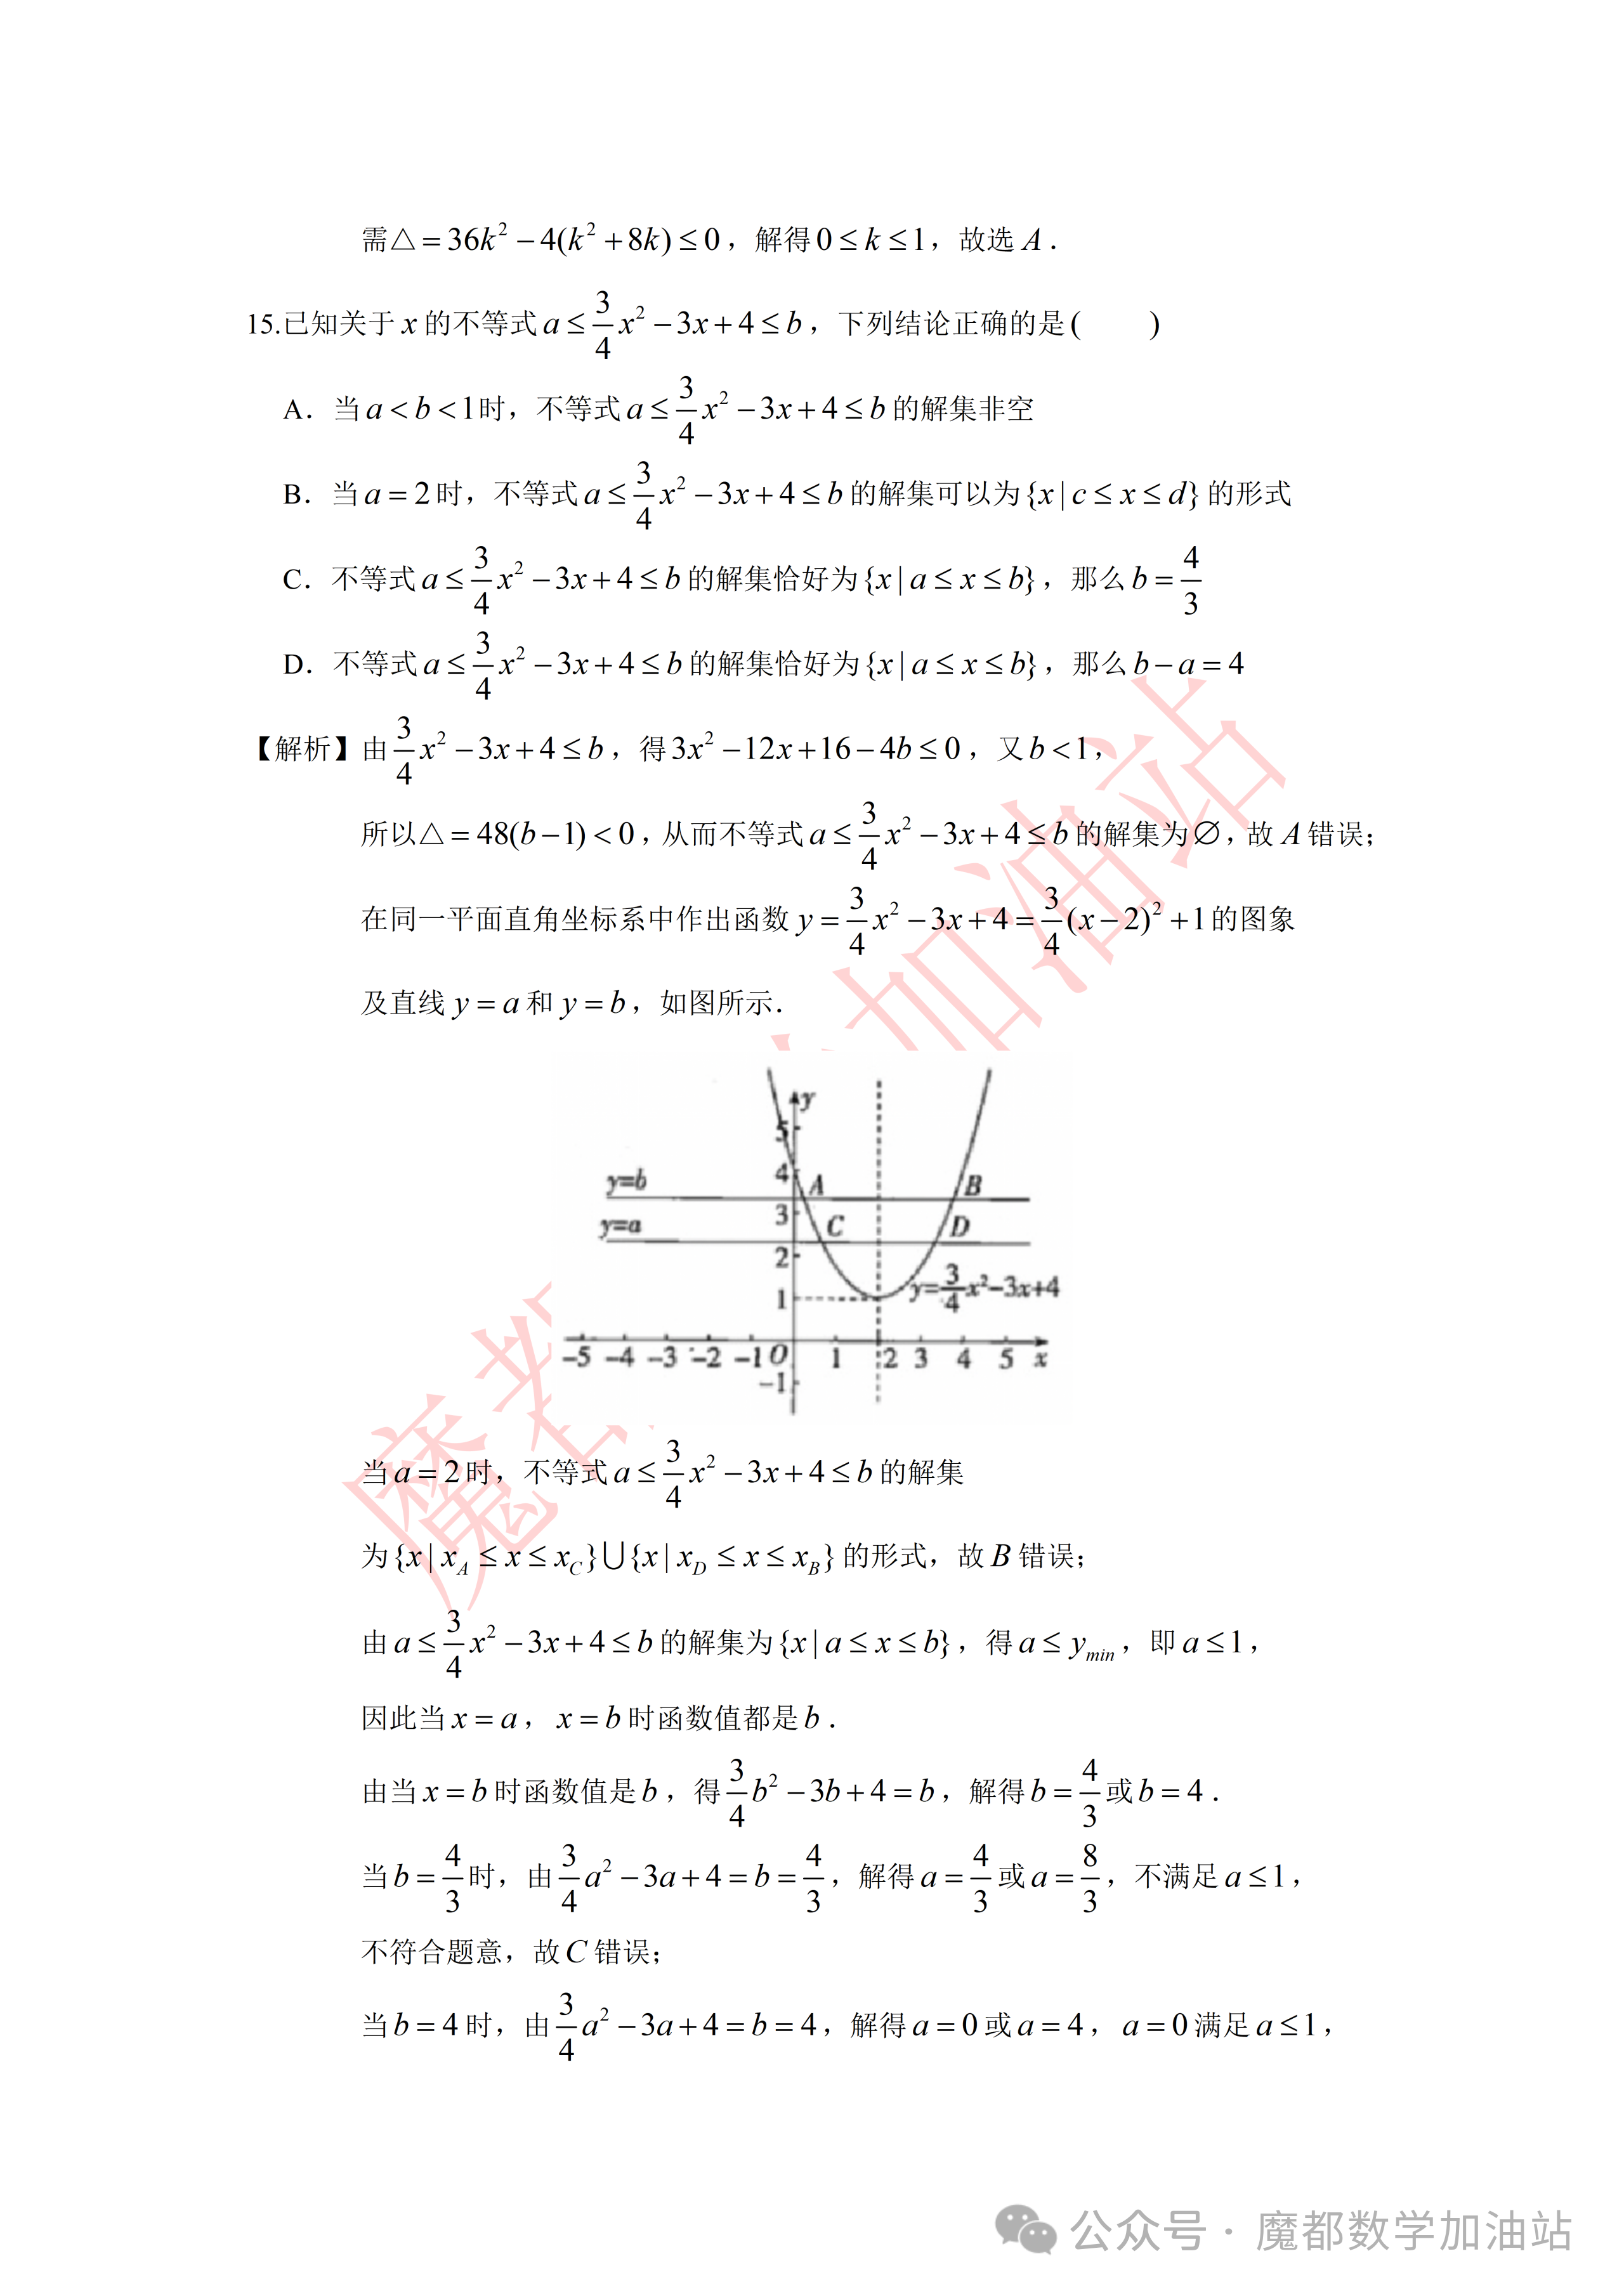
\includegraphics[width=.55\linewidth,trim=900bp 1400bp 760bp 1680bp,clip]{../原图/高一46_交附闵行_国庆作业3/05.png}
\end{center}
\step{当 $a=2$ 时，不等式 $a\leqslant\dfrac34x^2-3x+4\leqslant b$ 的解集为
$\{x\mid x_A\leqslant x\leqslant x_C\}\cup\{x\mid x_D\leqslant x\leqslant x_B\}$ 的形式，故 $B$ 错误；}
\step{由 $a\leqslant\dfrac34x^2-3x+4\leqslant b$ 的解集恰好为 $\{x\mid a\leqslant x\leqslant b\}$ 的形式，得 $a\leqslant y_{\min}$，即 $a\leqslant1$，}
\step{因为当 $x=a$、$x=b$ 时函数值都是 $b$，当 $x=a$ 时，$\dfrac34a^2-3a+4=b$；当 $x=b$ 时，$\dfrac34b^2-3b+4=b$，}
\step{解得 $b=\dfrac43$ 或 $b=4$，}
\step{当 $b=\dfrac43$ 时，由 $\dfrac34a^2-3a+4=b$，解得 $a=\dfrac43$ 或 $a=\dfrac83$，不符合题意，故 $C$ 错误；}
\step{当 $b=4$ 时，由 $\dfrac34a^2-3a+4=b$，解得 $a=0$ 或 $a=4$，$a=0$ 满足 $a\leqslant1$，故 $D$ 正确；}
\step{故选 $D$.}
\solend
\fi

\item 已知 $x$、$y\in(0,+\infty)$，则 $(x-y)^2+2y+1-x+\dfrac4x$ 的最小值为\mbox{（\quad）}

\keepwithprev
A. $1$\qquad B. $2$\qquad C. $3$\qquad D. $4$

\ans{$D$}

\ifanswer
\solbegin
\step{因为 $(x-y)^2+2y+1-x+\dfrac4x=(x-y-1)^2+x+\dfrac4x$，}
\step{当且仅当 $x-y-1=0$，且 $x=\dfrac4x$ 时取等号，}
\step{又因为 $x+\dfrac4x\geqslant2\sqrt{x\cdot\dfrac4x}=4$，当且仅当 $x=2$ 时取等号，}
\step{故选 $D$.}
\solend
\fi

\end{enumerate}

\bigsec{三、解答题}

\begin{enumerate}
\setcounter{enumi}{16}

\item 设集合 $A=\left\{x\middle|\dfrac{x-3}{x-1}<0\right\}$，$B=\{x\mid x^2-2ax+a^2-1>0\}$.
\begin{enumerate}[label=(\arabic*)]
\item 若 $a=3$，求 $A\cup B$；
\item 若“$x\in A$”是“$x\in B$”的充分条件，求实数 $a$ 的取值范围.
\end{enumerate}

\ifanswer
\solbegin
% 注：原卷题干为 a^2-1，故 a=3 时常数项为 8；题干与本步一致。
\stepm{(1)}{当 $a=3$ 时，$B=\{x\mid x^2-6x+8>0\}=\{x\mid x<2\text{ 或 }x>4\}$；}
\step{因为 $A=\left\{x\middle|\dfrac{x-3}{x-1}<0\right\}=\{x\mid(x-1)(x-3)<0\}=\{x\mid1<x<3\}$，}
\step{所以 $A\cup B=\{x\mid x<2\text{ 或 }x>4\}\cup\{x\mid1<x<3\}
=\{x\mid x<3\text{ 或 }x>4\}$.}
\stepm{(2)}{因为“$x\in A$”是“$x\in B$”的充分条件，所以 $A\subseteq B$，}
\step{因 $A=\left\{x\middle|\dfrac{x-3}{x-1}<0\right\}
=\{x\mid(x-1)(x-3)<0\}=\{x\mid1<x<3\}$，}
\step{所以 $A\subseteq B=\{x\mid x<a-1\text{ 或 }x>a+1\}$，}
\step{要使 $A\subseteq B$，需有 $a-1\geqslant3$ 或 $a+1\leqslant1$，}
\step{所以 $a\geqslant4$ 或 $a\leqslant0$，故 $a$ 的取值范围为 $\{a\mid a\geqslant4\text{ 或 }a\leqslant0\}$.}
\solend
\fi

\ansspace[6]

\item 某学校引入种植类劳动教育课程，打算围成如图所示的四块全等的长方形田地种植不同种类的蔬菜，其中一面可以利用原有的墙（足够长），其他各面需要用篱笆围成，设其中一块田地为矩形 $ABCD$.

\begin{center}
% 原图第 6 页配图直接裁取。
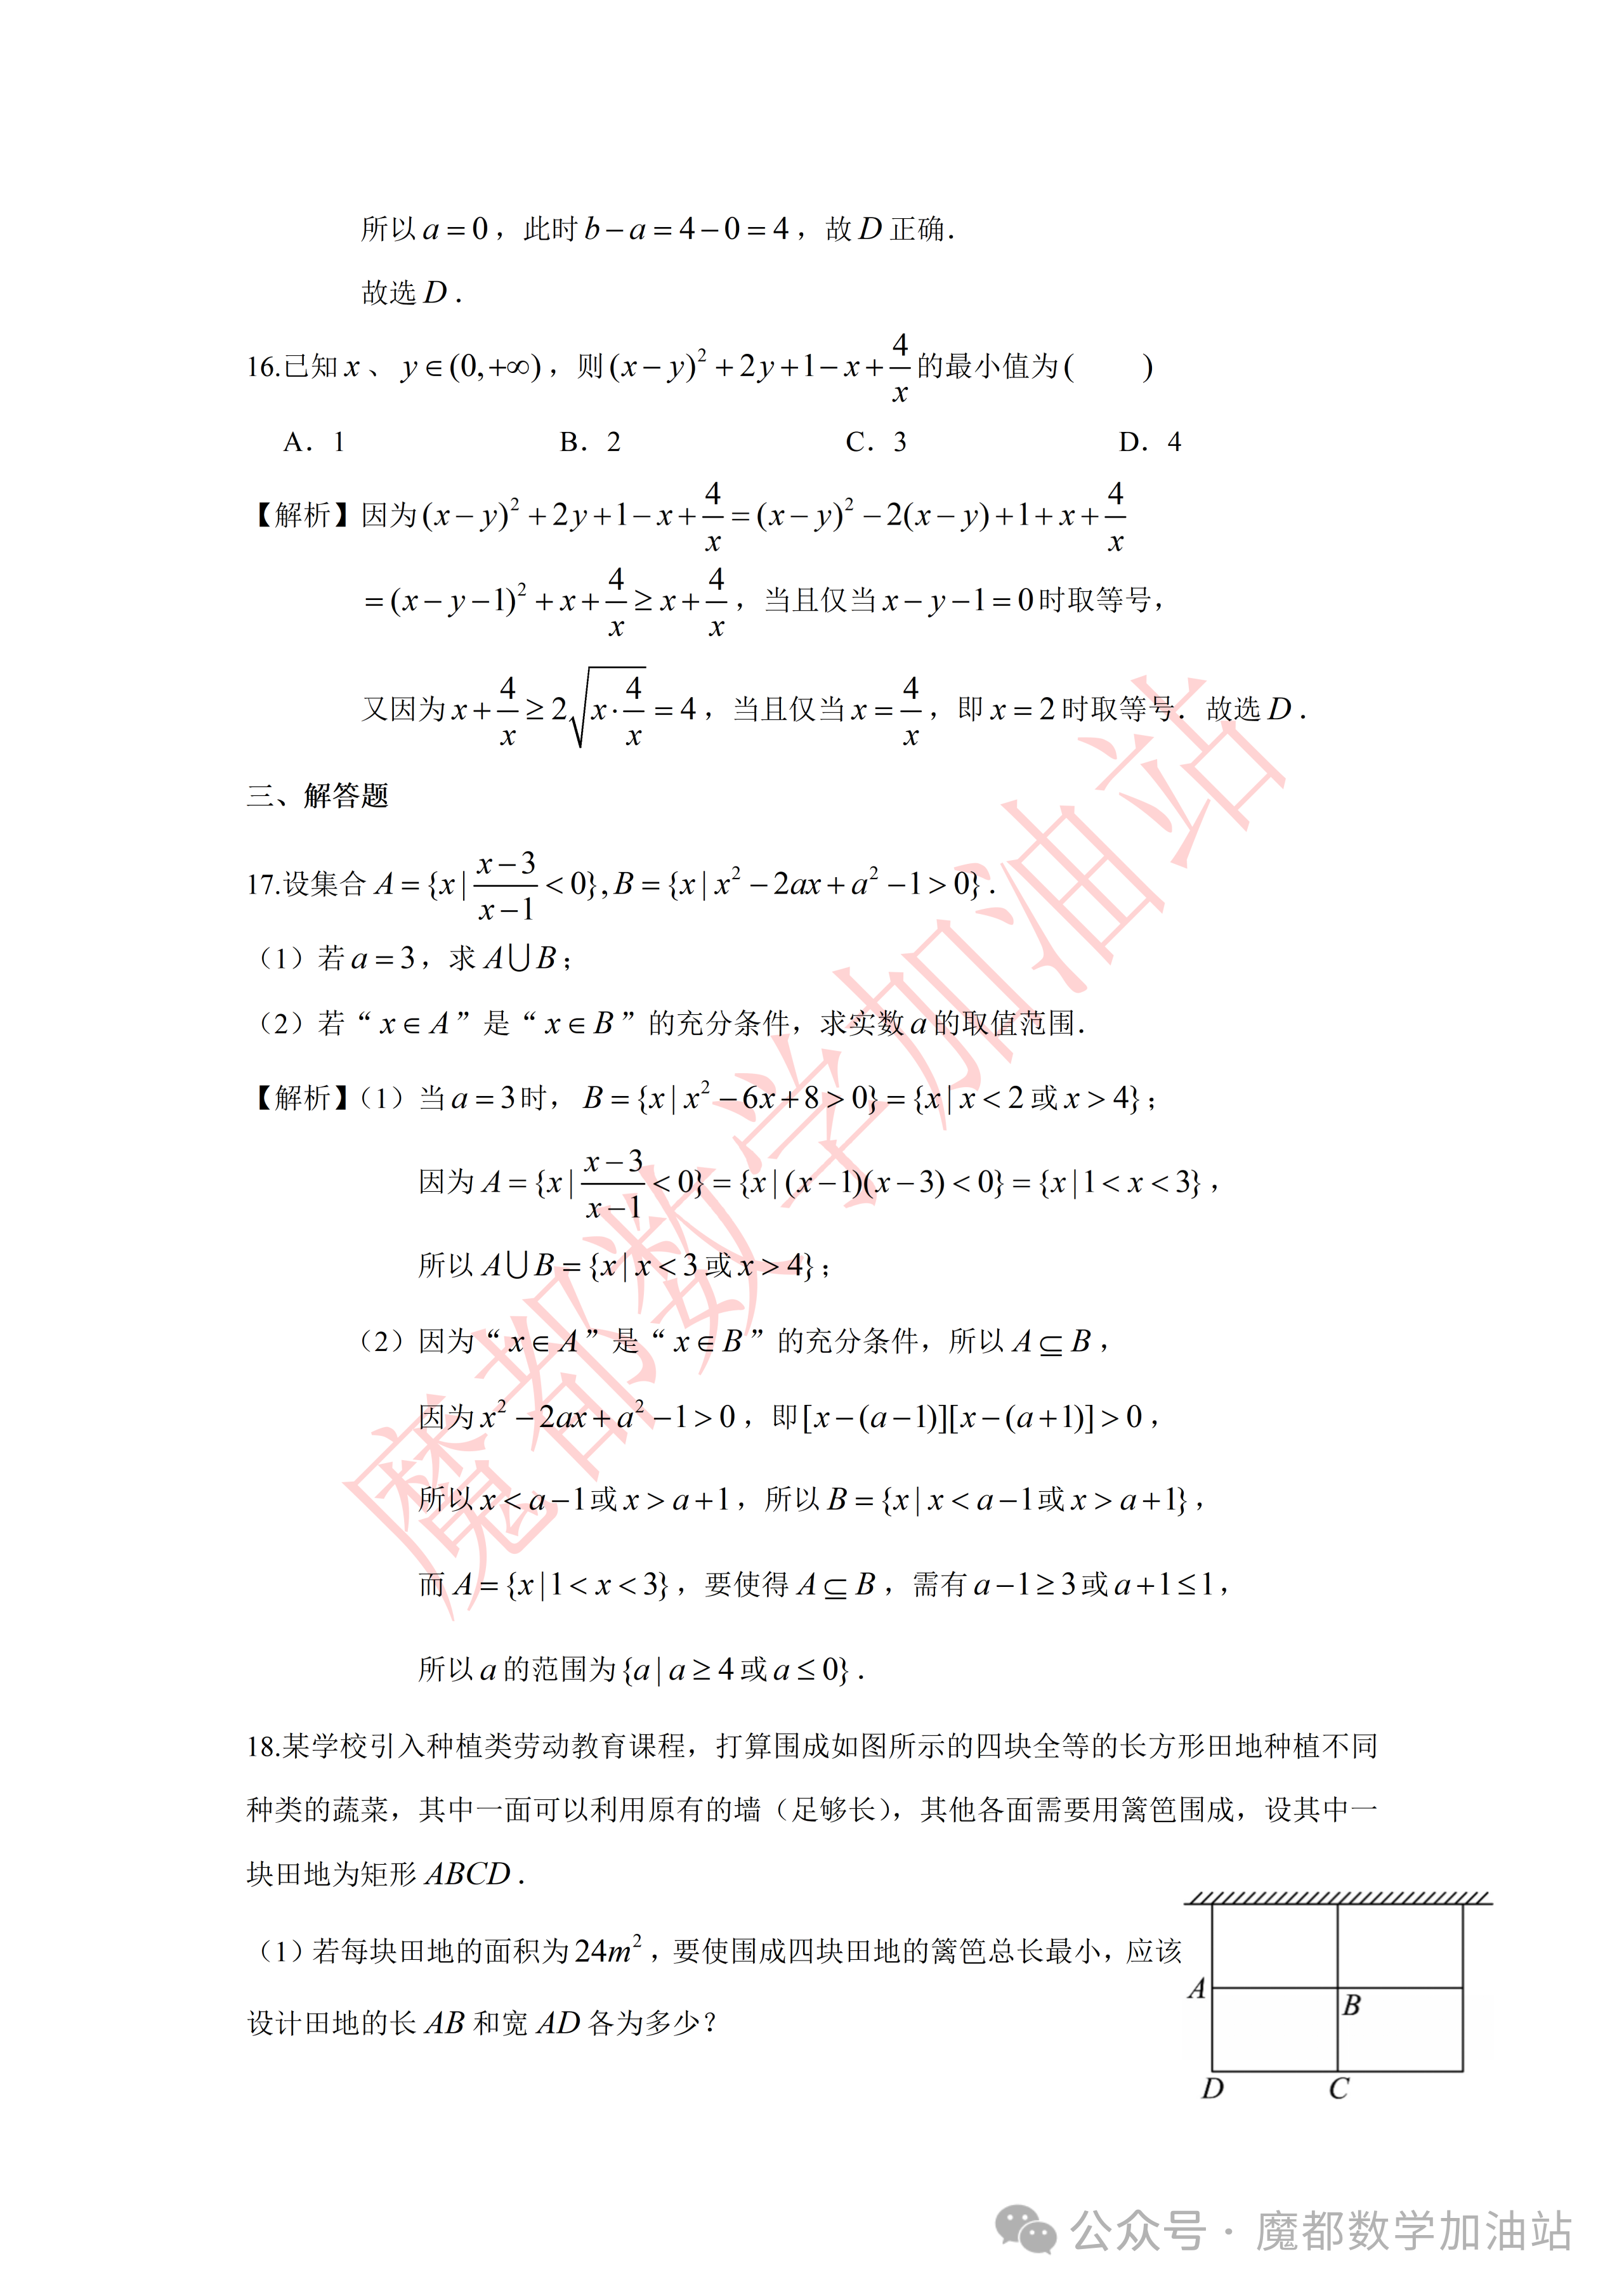
\includegraphics[width=.33\linewidth,trim=1866bp 220bp 210bp 2960bp,clip]{../原图/高一46_交附闵行_国庆作业3/06.png}
\end{center}

\begin{enumerate}[label=(\arabic*)]
\item 若每块田地的面积为 $24\,\text{m}^2$，要使围成四块田地的篱笆总长最小，应该设计田地的长 $AB$ 和宽 $AD$ 各为多少？
\item 现有 $40\,\text{m}$ 长的篱笆，要使每块田地的面积最大，应该设计田地的长 $AB$ 和宽 $AD$ 各为多少？
\end{enumerate}

\ifanswer
\solbegin
\stepm{(1)}{设 $AB$ 长为 $x\,\text{m}$，$AD$ 宽为 $y\,\text{m}$，由题意得 $xy=24$，篱笆总长为 $4x+6y$，}
\step{$4x+6y\geqslant2\sqrt{4x\cdot6y}=2\sqrt{24xy}=48$，}
\step{当且仅当 $4x=6y$ 时取等号，解得 $x=6$，$y=4$，}
\step{所以田地的长 $AB$ 为 $6\,\text{m}$，宽 $AD$ 为 $4\,\text{m}$.}
\stepm{(2)}{设 $AB$ 长为 $a\,\text{m}$，$AD$ 宽为 $b\,\text{m}$，由篱笆总长 $4a+6b=40$，即 $2a+3b=20$，}
\step{将 $a=\dfrac{20-3b}{2}$ 代入每块田地面积 $ab$，得 $ab=\dfrac12b(20-3b)=-\dfrac32b^2+10b$，}
\step{当 $b=\dfrac{10}{3}$ 时，$ab$ 最大，此时 $a=5$，}
\step{所以田地的长 $AB$ 为 $5\,\text{m}$，宽 $AD$ 为 $\dfrac{10}{3}\,\text{m}$.}
\solend
\fi

\ansspace[8]

\item 已知 $x_1$、$x_2$ 是一元二次方程 $4kx^2-4kx+k+1=0$ 的两个不等实数根.
\begin{enumerate}[label=(\arabic*)]
\item 若 $x_1$、$x_2$ 均为正根，求实数 $k$ 的取值范围；
\item 求使 $\dfrac{x_1}{x_2}+\dfrac{x_2}{x_1}-2$ 的值为整数 $k$ 的整数值.
\end{enumerate}

\ifanswer
\solbegin
\stepm{(1)}{由题意，$x_1$、$x_2$ 是方程 $4kx^2-4kx+k+1=0$ 的两个不等实数根，}
\step{故 $k\neq0$，$\Delta=(-4k)^2-16k(k+1)>0$，得 $-16k>0$，所以 $k<0$，}
\step{又 $x_1+x_2=1$，$x_1x_2=\dfrac{k+1}{4k}>0$，得 $k+1<0$，}
\step{所以 $k$ 的取值范围为 $(-\infty,-1)$.}
\stepm{(2)}{由题意，}
\step{$\dfrac{x_1}{x_2}+\dfrac{x_2}{x_1}-2
=\dfrac{x_1^2+x_2^2-2x_1x_2}{x_1x_2}
=\dfrac{(x_1+x_2)^2-4x_1x_2}{x_1x_2}$，}
\step{又 $x_1+x_2=1$，$x_1x_2=\dfrac{k+1}{4k}$，}
\step{则 $\dfrac{x_1}{x_2}+\dfrac{x_2}{x_1}-2=-\dfrac4{k+1}$，}
\step{由于 $-\dfrac4{k+1}$ 为整数，故 $k+1$ 只能取 $\pm1$、$\pm2$、$\pm4$，又 $k<-1$，}
\step{所以整数 $k$ 的值为 $-2$、$-3$、$-5$.}
\solend
\fi

\ansspace[8]

\item 已知 $a>0$，$b>0$，且 $2a+3b=3$.
\begin{enumerate}[label=(\arabic*)]
\item 求 $ab$ 的最大值；
\item 求 $a-\dfrac1{6b}$ 的最大值；
\item 求 $\dfrac2a+\dfrac3{b+1}$ 的最小值.
\end{enumerate}

\ifanswer
\solbegin
\stepm{(1)}{由 $2a+3b=3$，得 $3=2a+3b\geqslant2\sqrt{6ab}$，}
\step{所以 $ab\leqslant\dfrac38$，当且仅当 $2a=3b=\dfrac32$ 时取等号，}
\step{故 $ab$ 的最大值为 $\dfrac38$.}
\stepm{(2)}{由 $2a+3b=3$，得 $a=\dfrac32-\dfrac32b$，}
\step{则 $a-\dfrac1{6b}=\dfrac32-\dfrac32b-\dfrac1{6b}$，}
\step{由基本不等式，$\dfrac32b+\dfrac1{6b}\geqslant2\sqrt{\dfrac32b\cdot\dfrac1{6b}}=1$，}
\step{当且仅当 $\dfrac32b=\dfrac1{6b}$，即 $b=\dfrac13$、$a=1$ 时取等号，}
\step{所以 $a-\dfrac1{6b}$ 的最大值为 $\dfrac12$.}
\stepm{(3)}{由 $2a+3b=3$，得 $2a+3(b+1)=6$，}
\step{$\dfrac2a+\dfrac3{b+1}
=\dfrac16\left(2a+3(b+1)\right)\left(\dfrac2a+\dfrac3{b+1}\right)$}
\step{$=\dfrac16\left(13+\dfrac{6(b+1)}a+\dfrac{6a}{b+1}\right)
\geqslant\dfrac16\left(13+2\sqrt{\dfrac{6(b+1)}a\cdot\dfrac{6a}{b+1}}\right)=\dfrac{25}{6}$，}
\step{当且仅当 $a=b+1$，即 $a=\dfrac65$、$b=\dfrac15$ 时取等号，}
\step{所以 $\dfrac2a+\dfrac3{b+1}$ 的最小值为 $\dfrac{25}{6}$.}
\solend
\fi

\ansspace[8]

\item 已知 $U=\R$ 为全集，集合 $A=\{s^2+3t^2\mid s,t\in U\}$.
\begin{enumerate}[label=(\arabic*)]
\item 设 $U=\{1,3,5\}$，求集合 $A$ 的元素个数；
\item 设 $U=\Z$，证明：若 $x\in A$，则 $7x\in A$；
\item 设 $U=\R$，$x$、$y\in A$，且 $x=m^2+3n^2$，$y=p^2+3q^2$，若 $mp-3nq=\sqrt3$，求 $x+y+mq+np$ 的最小值.
\end{enumerate}

\ifanswer
\solbegin
\stepm{(1)}{当 $s=1$，$t=1$ 时，$s^2+3t^2=1+3=4$；}
\step{当 $s=1$，$t=3$ 时，$s^2+3t^2=1+27=28$；}
\step{当 $s=1$，$t=5$ 时，$s^2+3t^2=1+75=76$；}
\step{当 $s=3$，$t=1$ 时，$s^2+3t^2=9+3=12$；}
\step{当 $s=3$，$t=3$ 时，$s^2+3t^2=9+27=36$；}
\step{当 $s=3$，$t=5$ 时，$s^2+3t^2=9+75=84$；}
\step{当 $s=5$，$t=1$ 时，$s^2+3t^2=25+3=28$；}
\step{当 $s=5$，$t=3$ 时，$s^2+3t^2=25+27=52$；}
\step{当 $s=5$，$t=5$ 时，$s^2+3t^2=25+75=100$，}
\step{所以 $A=\{4,12,28,36,52,76,84,100\}$，有 $8$ 个元素.}
\stepm{(2)}{因为 $U=\Z$，$x\in A$，设 $x=s^2+3t^2$，}
\step{则 $7x=7(s^2+3t^2)=(2s+3t)^2+3(s-2t)^2\in A$，}
\step{所以 $7x\in A$.}
\stepm{(3)}{因为 $x=m^2+3n^2$，$y=p^2+3q^2$，}
\step{$xy=(m^2+3n^2)(p^2+3q^2)=3(mq+np)^2+(mp-3nq)^2$，}
\step{设 $mq+np=b$，则 $xy=3b^2+3$，所以 $y=\dfrac{3b^2+3}{x}$，}
\step{于是 $x+y+mq+np=x+\dfrac{3b^2+3}{x}+b\geqslant2\sqrt{3b^2+3}+b$，}
\step{设 $2\sqrt{3b^2+3}+b=t$，整理得 $11b^2+2bt+12-t^2=0$，}
\step{判别式法，$\Delta=4t^2-44(12-t^2)\geqslant0$，得 $t\geqslant\sqrt{11}$，}
\step{即 $(x+y+mq+np)_{\min}=\sqrt{11}$，所以 $x+y+mq+np$ 的最小值为 $\sqrt{11}$.}
\solend
\fi

\ansspace*[10]

\end{enumerate}

\end{document}
"
% 紧凑版：xelatex "\def\iscompact{1}% 高一46_交附闵行_国庆作业3.tex
%   —— 高一上数学“2026-2027 年交附闵行高一上国庆作业 3”（讲评版）
% 试卷版：xelatex 高一46_交附闵行_国庆作业3.tex
% 答案版：xelatex "\def\isanswer{1}% 高一46_交附闵行_国庆作业3.tex
%   —— 高一上数学“2026-2027 年交附闵行高一上国庆作业 3”（讲评版）
% 试卷版：xelatex 高一46_交附闵行_国庆作业3.tex
% 答案版：xelatex "\def\isanswer{1}\input{高一46_交附闵行_国庆作业3.tex}"
% 紧凑版：xelatex "\def\iscompact{1}\input{高一46_交附闵行_国庆作业3.tex}"
%
% 原始材料：微信公众号“魔都数学加油站”，作者破晓，2026-10-02 17:56 发布。
% 原文标题：“27学年高一46——2026-2027你那上海市交附闵行高一上国庆作业3”
% （公众号标题中的“你那”照录，系原文标题字样）；原文链接：
% http://mp.weixin.qq.com/s?__biz=Mzg4ODU1ODMxOQ==&mid=2247591657&idx=3&sn=a894d1a16611283a61b3eaba32a3f24c&chksm=cee83366c6a55381b370069f84ef63d20251f94608bb37cc4ec2d66227401bd147f4f6bd8256&scene=126&sessionid=1790935402&subscene=7&clicktime=1790937618&enterid=1790937618#rd
% 正文为 9 张 PNG 页，按页序读取原图；第 01、02、07 页 4762×6735，
% 第 03—06、08、09 页 2560×3620。卷面标题照原卷印作“2026-2027 年交附闵行高一上国庆作业 3”。
% 原文从第 3 题起，题号照原卷保留；正文为讲评版，答案、解析依原卷顺序录入。
% 水印及页脚公众号标识不录入。卷面插图直接裁取对应原图页，不另制图片文件。
%
% 与原卷的排版差异：
%   ① 原卷按“一、填空题”“二、选择题”“三、解答题”分节，本稿沿用原节与原题号，
%      只改排为全稿统一的大节样式；
%   ② 原卷答案与解析依页面位置分布，本稿按 common.sty 统一置于答案版；
%   ③ 原卷副标题未印，本稿按“知识模块”口径标作“集合与常用逻辑用语、不等式”。
%
% 原卷存疑一处（照抄未改，见第 12 题题干及解析处注释）：
%   第 12 题题干同时给出 x∈Z，却称不等式组有“50 个不等的实数解”；解析按整数根计数。
%   此处题干与解析的原文不一致，本稿均照录。
% 第 17 题曾疑似有常数项不一致：复核原图题干为 a^2-1，a=3 时常数项确为 8，
% 与解析相符；不将其记作原卷错误。
%
\documentclass[a4paper,11pt]{article}
\usepackage{common}

\begin{document}

\examtitlest[3]{2026--2027 年交附闵行高一上国庆作业 3}{集合与常用逻辑用语、不等式}

\bigsec{一、填空题}

\begin{enumerate}
\setcounter{enumi}{2}

\item 不等式 $\dfrac{x^2-10}{x+2}\geqslant1$ 的解集为\blankline[4.4em].

\ifanswer
\ans{$\{x\mid-3\leqslant x<-2\text{ 或 }x\geqslant4\}$}
\solbegin
\step{不等式 $\dfrac{x^2-10}{x+2}\geqslant1$，移项得 $\dfrac{x^2-10}{x+2}-1\geqslant0$，}
\step{通分得 $\dfrac{x^2-x-12}{x+2}\geqslant0$，即 $\dfrac{(x-4)(x+3)}{x+2}\geqslant0$，}
\step{解得 $-3\leqslant x<-2$ 或 $x\geqslant4$，}
\step{故不等式的解集为 $\{x\mid-3\leqslant x<-2\text{ 或 }x\geqslant4\}$.}
\solend
\fi

\item $|x-3|+|x-5|\geqslant2$，当等号成立时，$x$ 的范围是\blankline[4.4em].

\ifanswer
\ans{$[3,5]$}
\fi

\item 若直角三角形斜边长等于 $4\sqrt2\,\text{cm}$，则直角三角形面积的最大值为\blankline[4.4em].

\ifanswer
\solbegin
\step{设 $Rt\triangle ABC$ 中，$C=90^\circ$，则 $c=\sqrt{a^2+b^2}=4\sqrt2$，所以 $a^2+b^2=32$，}
\step{由基本不等式得 $a^2+b^2\geqslant2ab$，当且仅当 $a=b=4$ 时取等号，}
\step{所以 $\triangle ABC$ 的面积 $S=\dfrac12ab\leqslant8$，}
\step{当且仅当 $a=b=4$ 时，$\triangle ABC$ 的面积最大值为 $8$.}
\solend
\fi

\item 不等式 $(x-1)(2-x)>0$ 的解集为\blankline[4.4em].

\ifanswer
\solbegin
\step{$(x-1)(2-x)>0\Rightarrow(x-1)(x-2)<0$，}
\step{故不等式的解集为 $\{x\mid1<x<2\}$.}
\solend
\fi

\item 已知集合 $A=\{1,2\}$，$B=\{x\mid x^2-2mx+m=0\}$，$A\cup B=A$，则实数 $m$ 的取值范围为\blankline[4.4em].

\ifanswer
\solbegin
\step{因为 $A\cup B=A$，所以 $B\subseteq A$，}
\step{当 $B=\varnothing$ 时，$\Delta=(-2m)^2-4m<0$，解得 $0<m<1$，}
\step{当 $B$ 为单元素集时，$\Delta=0$，解得 $m=0$ 或 $m=1$，}
\step{当 $m=0$ 时，方程 $x^2=0$，解得 $x=0$，此时 $B=\{0\}$，不满足 $B\subseteq A$；}
\step{当 $m=1$ 时，方程 $x^2-2x+1=0$，解得 $x=1$，此时 $B=\{1\}$，满足 $B\subseteq A$；}
\step{当 $B=\{1,2\}$ 时，由韦达定理得 $1+2=2m$，$1\times2=m$，无解，}
\step{综上所述，实数 $m$ 的取值范围为 $\{m\mid0<m\leqslant1\}$.}
\solend
\fi

\item 设 $a$、$b$、$c\in\R^+$，若 $a+b+c=1$，则 $\dfrac1a+\dfrac1b+\dfrac1c\geqslant$\blankline[4.4em].

\ifanswer
\solbegin
\step{因为 $a$、$b$、$c\in\R^+$，且 $a+b+c=1$，}
\step{所以 $\dfrac1a+\dfrac1b+\dfrac1c=(a+b+c)\left(\dfrac1a+\dfrac1b+\dfrac1c\right)$}
\step{$=3+\dfrac ab+\dfrac ba+\dfrac ac+\dfrac ca+\dfrac bc+\dfrac cb$，}
\step{由基本不等式得 $\dfrac ab+\dfrac ba\geqslant2$，$\dfrac ac+\dfrac ca\geqslant2$，$\dfrac bc+\dfrac cb\geqslant2$，}
\step{所以 $\dfrac1a+\dfrac1b+\dfrac1c\geqslant9$，当且仅当 $a=b=c=\dfrac13$ 时取等号，}
\step{所以 $\dfrac1a+\dfrac1b+\dfrac1c$ 的最小值为 $9$.}
\solend
\fi

\item 已知 $-1\leqslant x+y\leqslant2$，$-2\leqslant x-y\leqslant1$，则 $x-2y$ 的范围为\blankline[4.4em].

\ifanswer
\solbegin
\step{设 $x-2y=m(x+y)+n(x-y)$，}
\step{则 $x-2y=(m+n)x+(m-n)y$，所以 $m+n=1$，$m-n=-2$，}
\step{解得 $m=-\dfrac12$，$n=\dfrac32$，}
\step{所以 $x-2y=-\dfrac12(x+y)+\dfrac32(x-y)$，}
\step{因为 $-1\leqslant x+y\leqslant2$，$-2\leqslant x-y\leqslant1$，}
\step{所以 $-4\leqslant x-2y\leqslant2$，即 $x-2y$ 的范围为 $[-4,2]$.}
\solend
\fi

\item 设集合 $A=\{1,2,m\}$，其中 $m$ 为实数，令 $B=\{a^2\mid a\in A\}$，$C=A\cup B$. 若 $C$ 中所有元素之和为 $6$，则 $C$ 中的所有元素之积为\blankline[4.4em].

\ifanswer
\solbegin
\step{因为 $A=\{1,2,m\}$，所以 $B=\{a^2\mid a\in A\}=\{1,4,m^2\}$，$m\neq1$，$m\neq2$，}
\step{又 $C=A\cup B$，所以 $1\in C$，$4\in C$，$m^2\in C$，}
\step{若 $m^2=1$，则 $m=-1$ 或 $m=1$（舍），当 $m=-1$ 时，$C=\{1,2,4,-1\}$，$C$ 中所有元素之和为 $6$，}
\step{此时 $C$ 中所有元素之积为 $-8$；}
\step{若 $m^2=2$，则 $m=-\sqrt2$ 或 $m=\sqrt2$，$C$ 中所有元素之和不符合题意；}
\step{若 $m^2=4$，则 $m=-2$ 或 $m=2$，此时 $C=\{1,2,4,-2\}$ 或 $C=\{1,2,4\}$，所有元素之和不符合题意；}
\step{若 $m^2\neq1$，$m^2\neq2$，$m^2\neq4$，则 $C=\{1,2,4,m,m^2\}$，}
\step{所以 $1+2+4+m+m^2=6$，即 $m^2+m+1=0$，无解，}
\step{综上所述，$C$ 中所有元素之积为 $-8$.}
\solend
\fi

\item 若对任意实数 $x>0$，$y>0$，不等式 $x+\sqrt{xy}\leqslant a(x+y)$ 恒成立，则实数 $a$ 的最小值为\blankline[4.4em].

\ifanswer
\solbegin
\step{由不等式 $x+\sqrt{xy}\leqslant a(x+y)$ 对任意实数 $x>0$，$y>0$ 恒成立，}
\step{得 $a\geqslant\dfrac{x+\sqrt{xy}}{x+y}$，}
\step{设 $\sqrt{\dfrac yx}=t>0$，则 $a\geqslant\dfrac{1+t}{1+t^2}$，}
\step{$\dfrac{1+t}{1+t^2}\leqslant\dfrac{\sqrt2+1}{2}$，当且仅当 $t=\sqrt2-1$ 时取等号，}
\step{所以实数 $a$ 的最小值为 $\dfrac{\sqrt2+1}{2}$.}
\solend
\fi

% 注：原卷题干给出 x∈Z，却写“实数解”；解析按整数解计数，题干与解析不一致，照录未改。
\item 若关于 $x$ 的不等式组
$\begin{cases}x^2-3mx\geqslant4m^2\\-20<x<120\end{cases}$（$x\in\Z,m>0$）恰有 $50$ 个不等的实数解，则 $m$ 的取值范围为\blankline[4.4em]（结果用区间表示）.

\ifanswer
\solbegin
\step{由 $x^2-3mx\geqslant4m^2$ 以及 $m>0$，解得 $x\leqslant-m$ 或 $x\geqslant4m$，}
\step{由原不等式组恰有 $50$ 个不等的实数解，可画出如下解集区间：}
\begin{center}
% 原图第 4 页数轴图直接裁取。
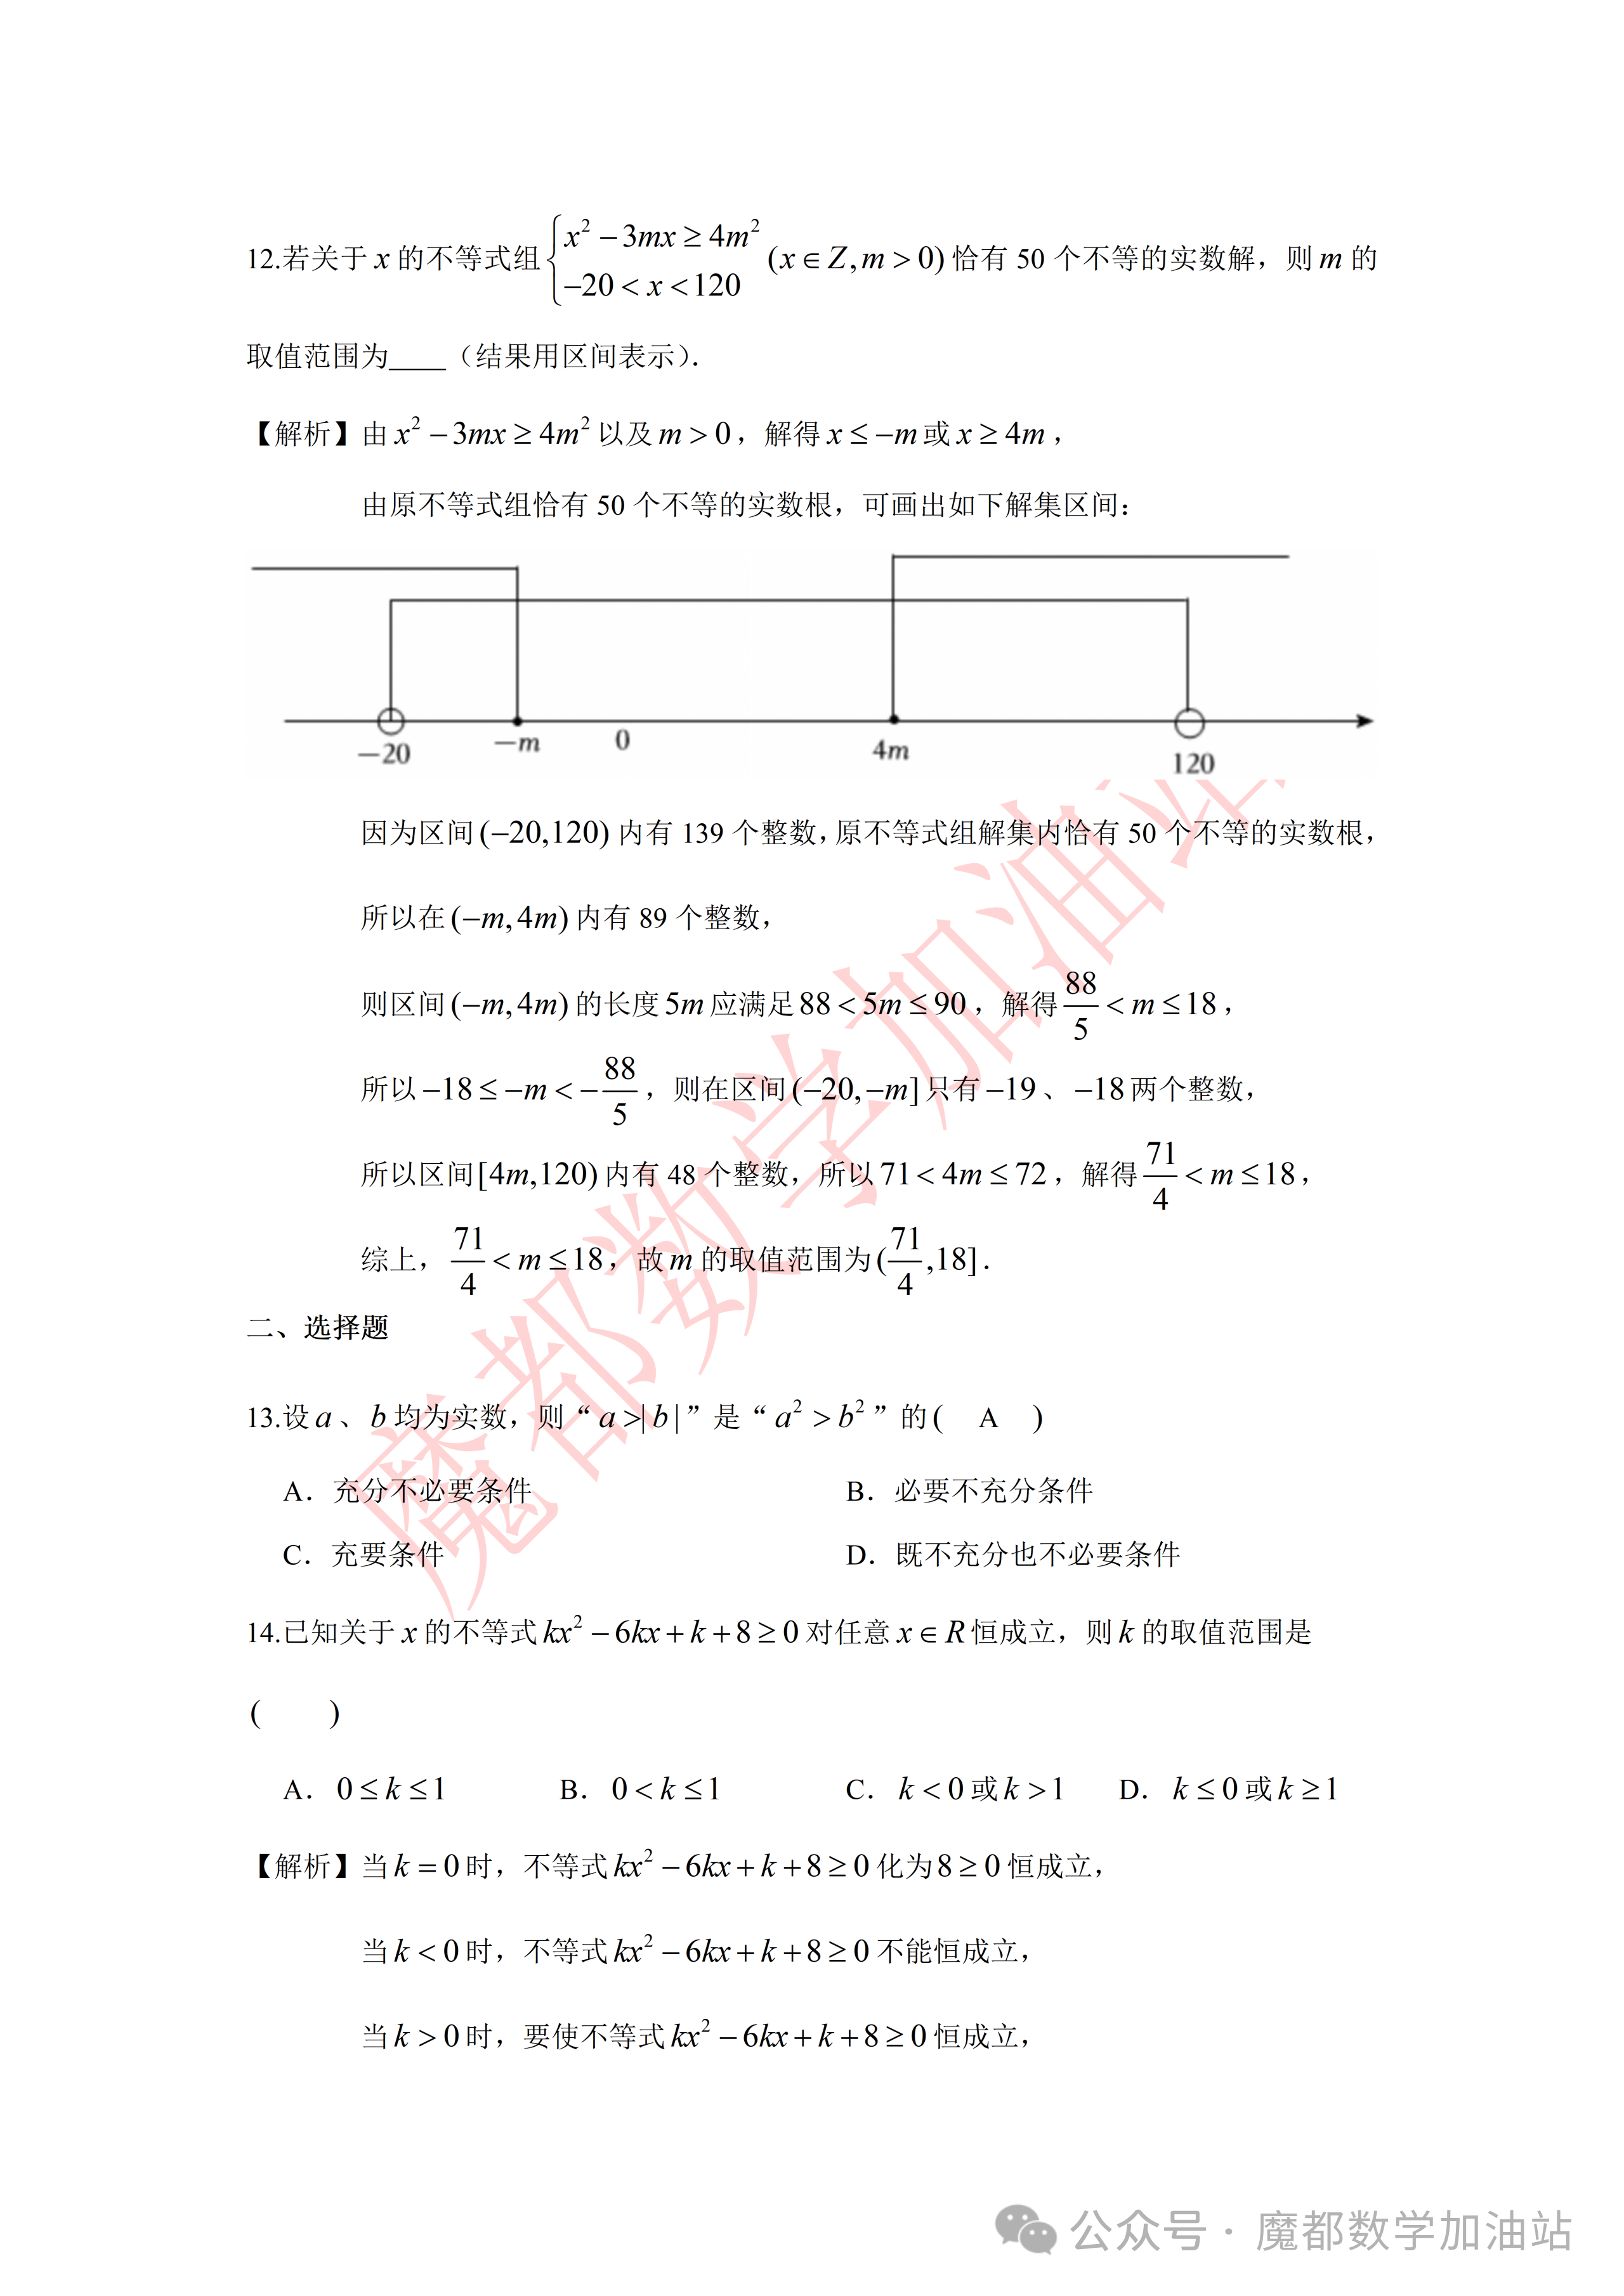
\includegraphics[width=.88\linewidth,trim=400bp 2410bp 320bp 860bp,clip]{../原图/高一46_交附闵行_国庆作业3/04.png}
\end{center}
\step{因为区间 $(-20,120)$ 内有 $139$ 个整数，原不等式组解集内有 $50$ 个不等的整数根，}
\step{所以在区间 $(-m,4m)$ 内有 $89$ 个整数，}
\step{则区间 $(-m,4m)$ 的长度 $5m$ 应满足 $88<5m\leqslant90$，解得 $\dfrac{88}{5}<m\leqslant18$，}
% 注：原卷题干称“实数解”，本行及后文按原卷解析照录为整数根计数。
\step{所以 $-18\leqslant-m<-\dfrac{88}{5}$，则在区间 $(-20,-m]$ 内有 $-19$、$-18$ 两个整数，}
\step{所以区间 $[4m,120)$ 内有 $48$ 个整数，}
\step{则 $71<4m\leqslant72$，解得 $\dfrac{71}{4}<m\leqslant18$，}
\step{综上，$\dfrac{71}{4}<m\leqslant18$，故 $m$ 的取值范围为 $\left(\dfrac{71}{4},18\right]$.}
\solend
\fi

\end{enumerate}

\bigsec{二、选择题}

\begin{enumerate}
\setcounter{enumi}{12}

\item 设 $a$、$b$ 均为实数，则“$a>|b|$”是“$a^2>b^2$”的\mbox{（\quad）}

\keepwithprev
A. 充分不必要条件\qquad B. 必要不充分条件

C. 充要条件\qquad\qquad D. 既不充分也不必要条件

\ans{$A$}

\item 已知关于 $x$ 的不等式 $kx^2-6kx+k+8\geqslant0$ 对任意 $x\in\R$ 恒成立，则 $k$ 的取值范围是\mbox{（\quad）}

\keepwithprev
A. $0\leqslant k\leqslant1$\qquad B. $0<k\leqslant1$

C. $k<0$ 或 $k>1$\qquad D. $k\leqslant0$ 或 $k\geqslant1$

\ans{$A$}

\ifanswer
\solbegin
\step{当 $k=0$ 时，不等式 $kx^2-6kx+k+8\geqslant0$ 化为 $8\geqslant0$ 恒成立，}
\step{当 $k<0$ 时，不等式 $kx^2-6kx+k+8\geqslant0$ 不能恒成立，}
\step{当 $k>0$ 时，要使不等式 $kx^2-6kx+k+8\geqslant0$ 恒成立，}
\step{需 $\Delta=36k^2-4(k^2+8k)\leqslant0$，解得 $0\leqslant k\leqslant1$，故选 $A$.}
\solend
\fi

\item 已知关于 $x$ 的不等式 $a\leqslant\dfrac34x^2-3x+4\leqslant b$，下列结论正确的是\mbox{（\quad）}

\keepwithprev
A. 当 $a<b<1$ 时，不等式 $a\leqslant\dfrac34x^2-3x+4\leqslant b$ 的解集非空

B. 当 $a=2$ 时，不等式 $a\leqslant\dfrac34x^2-3x+4\leqslant b$ 的解集可以为 $\{x\mid c\leqslant x\leqslant d\}$ 的形式

C. 不等式 $a\leqslant\dfrac34x^2-3x+4\leqslant b$ 的解集恰好为 $\{x\mid a\leqslant x\leqslant b\}$，那么 $b=\dfrac43$

D. 不等式 $a\leqslant\dfrac34x^2-3x+4\leqslant b$ 的解集恰好为 $\{x\mid a\leqslant x\leqslant b\}$，那么 $b-a=4$

\ans{$D$}

\ifanswer
\solbegin
\step{由 $\dfrac34x^2-3x+4\leqslant b$，得 $3x^2-12x+16-4b\leqslant0$，又 $b<1$，}
\step{所以 $\Delta=144-12(16-4b)=48(b-1)<0$，从而不等式无解，故 $A$ 错误；}
\step{在同一平面直角坐标系中作出函数 $y=\dfrac34x^2-3x+4=\dfrac34(x-2)^2+1$ 的图象及直线 $y=a$ 和 $y=b$，如图所示.}
\begin{center}
% 原图第 5 页解析配图直接裁取。
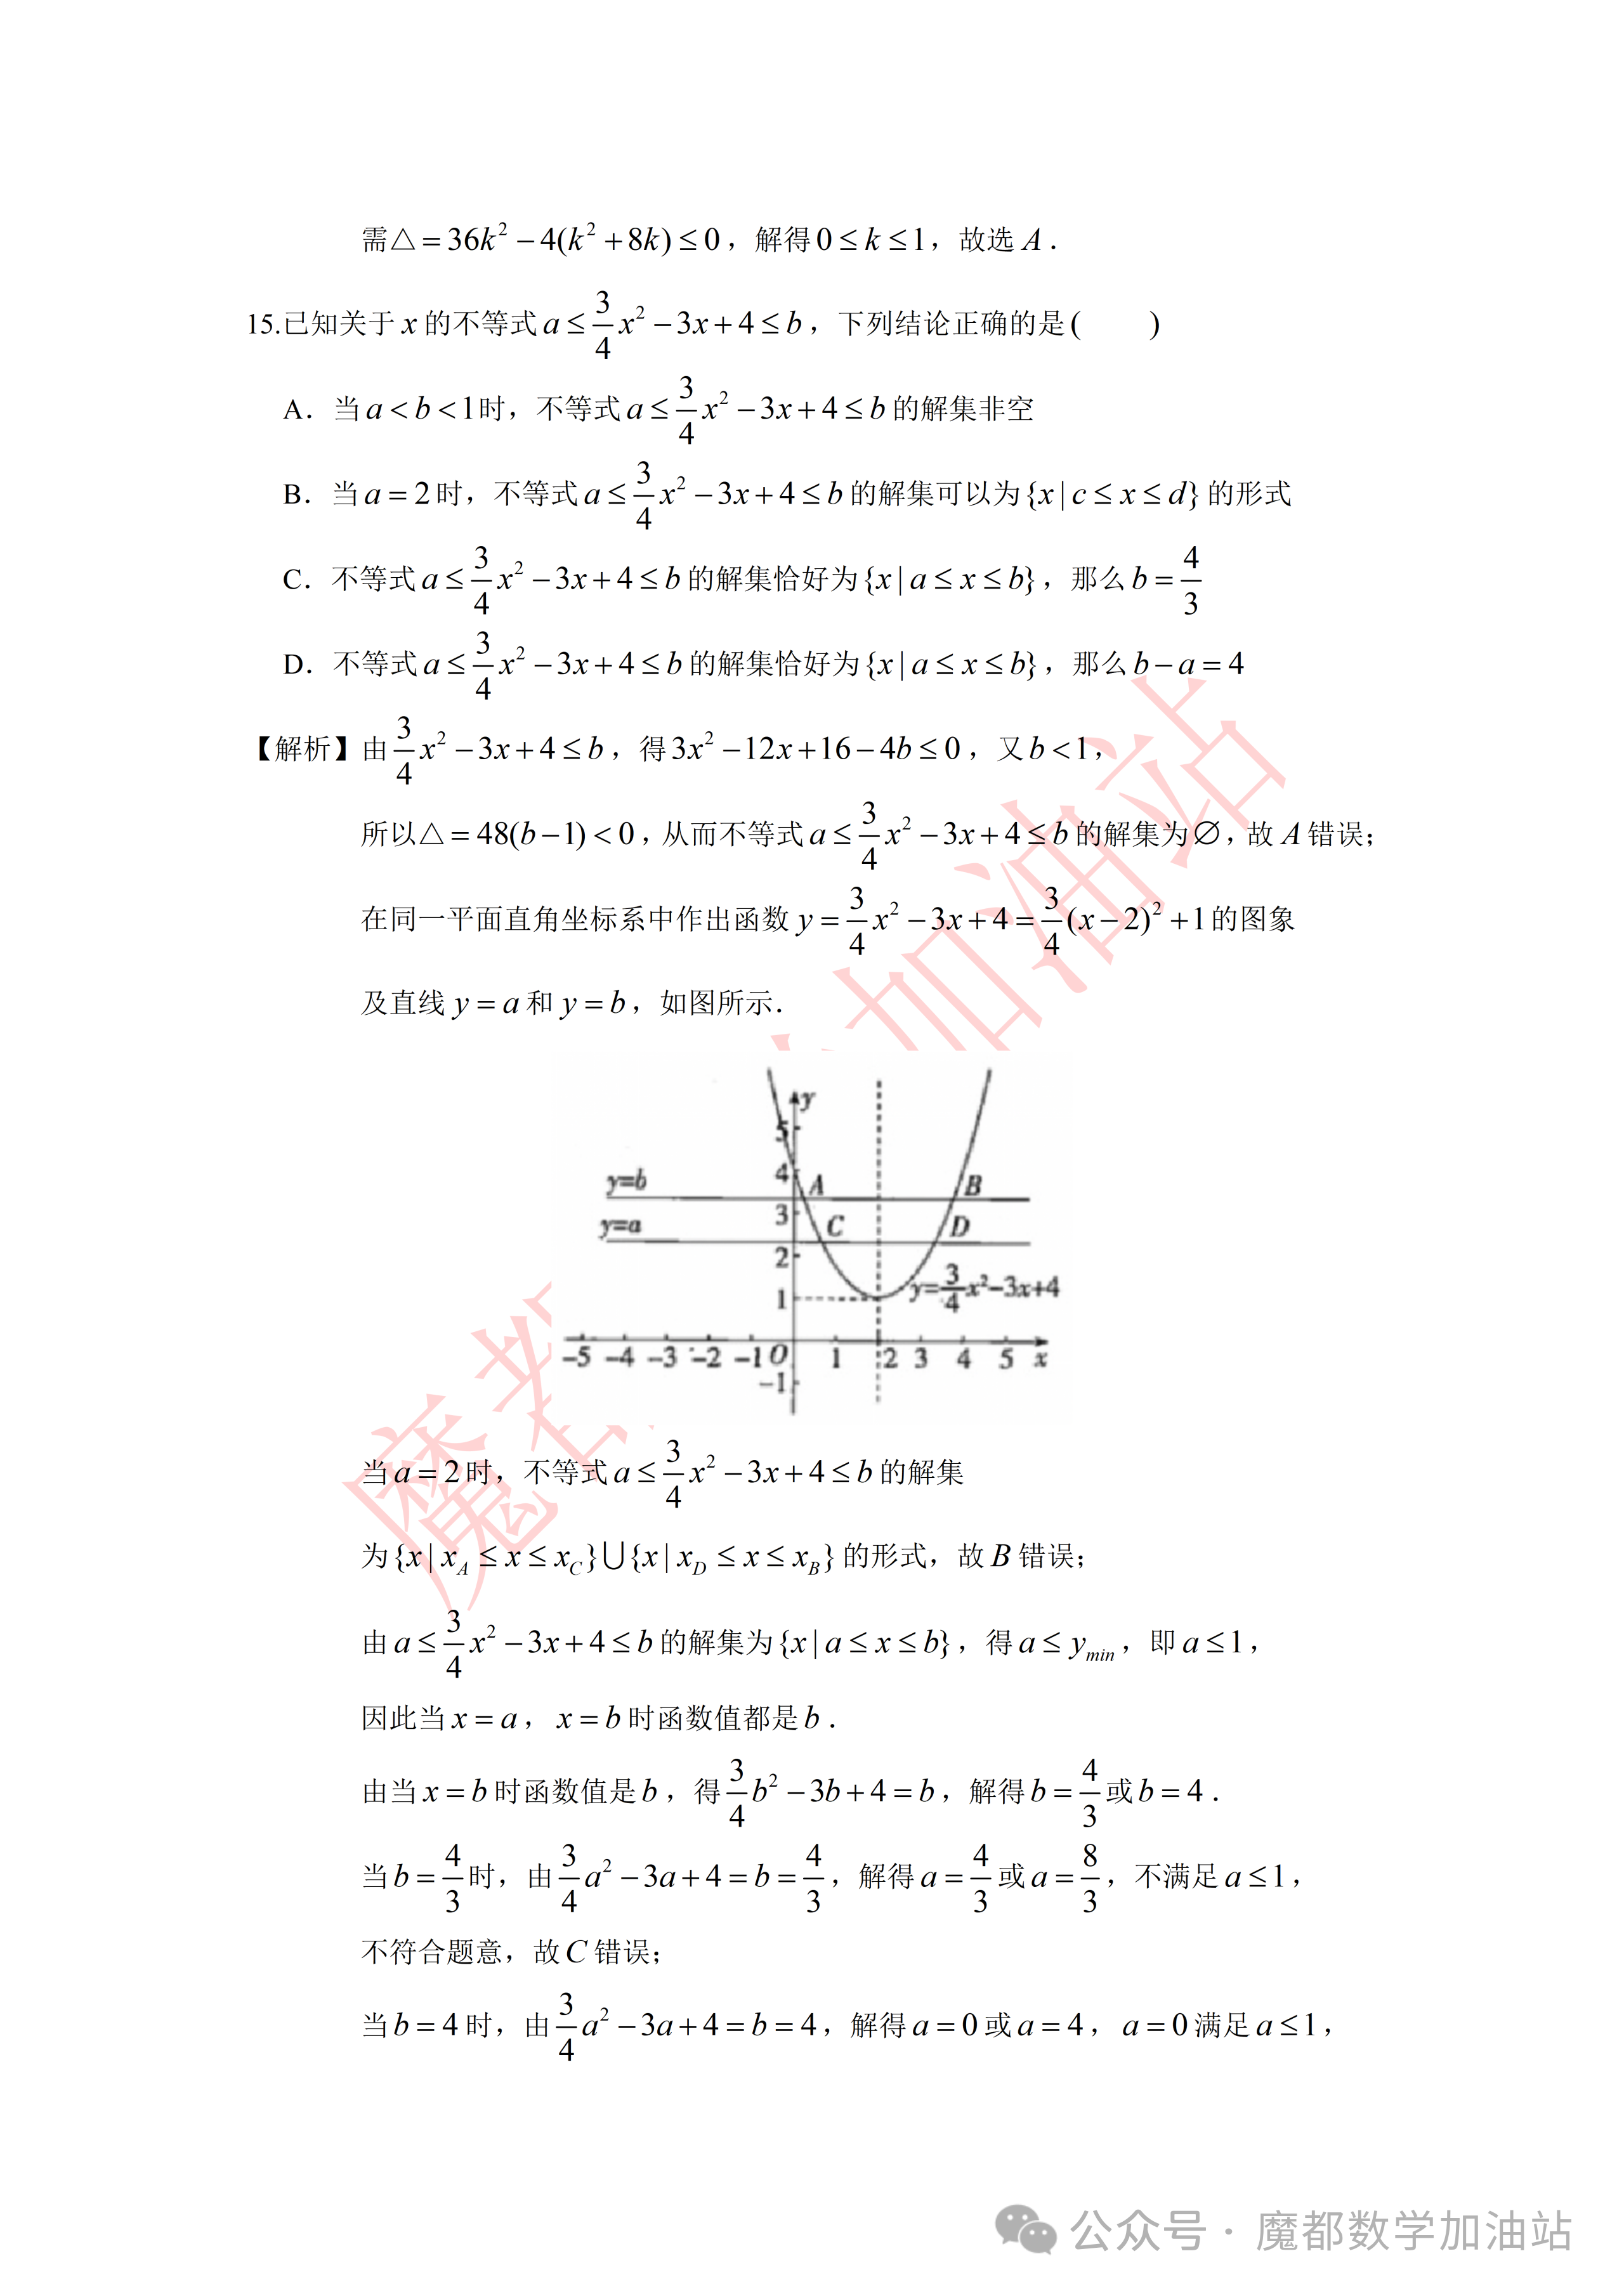
\includegraphics[width=.55\linewidth,trim=900bp 1400bp 760bp 1680bp,clip]{../原图/高一46_交附闵行_国庆作业3/05.png}
\end{center}
\step{当 $a=2$ 时，不等式 $a\leqslant\dfrac34x^2-3x+4\leqslant b$ 的解集为
$\{x\mid x_A\leqslant x\leqslant x_C\}\cup\{x\mid x_D\leqslant x\leqslant x_B\}$ 的形式，故 $B$ 错误；}
\step{由 $a\leqslant\dfrac34x^2-3x+4\leqslant b$ 的解集恰好为 $\{x\mid a\leqslant x\leqslant b\}$ 的形式，得 $a\leqslant y_{\min}$，即 $a\leqslant1$，}
\step{因为当 $x=a$、$x=b$ 时函数值都是 $b$，当 $x=a$ 时，$\dfrac34a^2-3a+4=b$；当 $x=b$ 时，$\dfrac34b^2-3b+4=b$，}
\step{解得 $b=\dfrac43$ 或 $b=4$，}
\step{当 $b=\dfrac43$ 时，由 $\dfrac34a^2-3a+4=b$，解得 $a=\dfrac43$ 或 $a=\dfrac83$，不符合题意，故 $C$ 错误；}
\step{当 $b=4$ 时，由 $\dfrac34a^2-3a+4=b$，解得 $a=0$ 或 $a=4$，$a=0$ 满足 $a\leqslant1$，故 $D$ 正确；}
\step{故选 $D$.}
\solend
\fi

\item 已知 $x$、$y\in(0,+\infty)$，则 $(x-y)^2+2y+1-x+\dfrac4x$ 的最小值为\mbox{（\quad）}

\keepwithprev
A. $1$\qquad B. $2$\qquad C. $3$\qquad D. $4$

\ans{$D$}

\ifanswer
\solbegin
\step{因为 $(x-y)^2+2y+1-x+\dfrac4x=(x-y-1)^2+x+\dfrac4x$，}
\step{当且仅当 $x-y-1=0$，且 $x=\dfrac4x$ 时取等号，}
\step{又因为 $x+\dfrac4x\geqslant2\sqrt{x\cdot\dfrac4x}=4$，当且仅当 $x=2$ 时取等号，}
\step{故选 $D$.}
\solend
\fi

\end{enumerate}

\bigsec{三、解答题}

\begin{enumerate}
\setcounter{enumi}{16}

\item 设集合 $A=\left\{x\middle|\dfrac{x-3}{x-1}<0\right\}$，$B=\{x\mid x^2-2ax+a^2-1>0\}$.
\begin{enumerate}[label=(\arabic*)]
\item 若 $a=3$，求 $A\cup B$；
\item 若“$x\in A$”是“$x\in B$”的充分条件，求实数 $a$ 的取值范围.
\end{enumerate}

\ifanswer
\solbegin
% 注：原卷题干为 a^2-1，故 a=3 时常数项为 8；题干与本步一致。
\stepm{(1)}{当 $a=3$ 时，$B=\{x\mid x^2-6x+8>0\}=\{x\mid x<2\text{ 或 }x>4\}$；}
\step{因为 $A=\left\{x\middle|\dfrac{x-3}{x-1}<0\right\}=\{x\mid(x-1)(x-3)<0\}=\{x\mid1<x<3\}$，}
\step{所以 $A\cup B=\{x\mid x<2\text{ 或 }x>4\}\cup\{x\mid1<x<3\}
=\{x\mid x<3\text{ 或 }x>4\}$.}
\stepm{(2)}{因为“$x\in A$”是“$x\in B$”的充分条件，所以 $A\subseteq B$，}
\step{因 $A=\left\{x\middle|\dfrac{x-3}{x-1}<0\right\}
=\{x\mid(x-1)(x-3)<0\}=\{x\mid1<x<3\}$，}
\step{所以 $A\subseteq B=\{x\mid x<a-1\text{ 或 }x>a+1\}$，}
\step{要使 $A\subseteq B$，需有 $a-1\geqslant3$ 或 $a+1\leqslant1$，}
\step{所以 $a\geqslant4$ 或 $a\leqslant0$，故 $a$ 的取值范围为 $\{a\mid a\geqslant4\text{ 或 }a\leqslant0\}$.}
\solend
\fi

\ansspace[6]

\item 某学校引入种植类劳动教育课程，打算围成如图所示的四块全等的长方形田地种植不同种类的蔬菜，其中一面可以利用原有的墙（足够长），其他各面需要用篱笆围成，设其中一块田地为矩形 $ABCD$.

\begin{center}
% 原图第 6 页配图直接裁取。
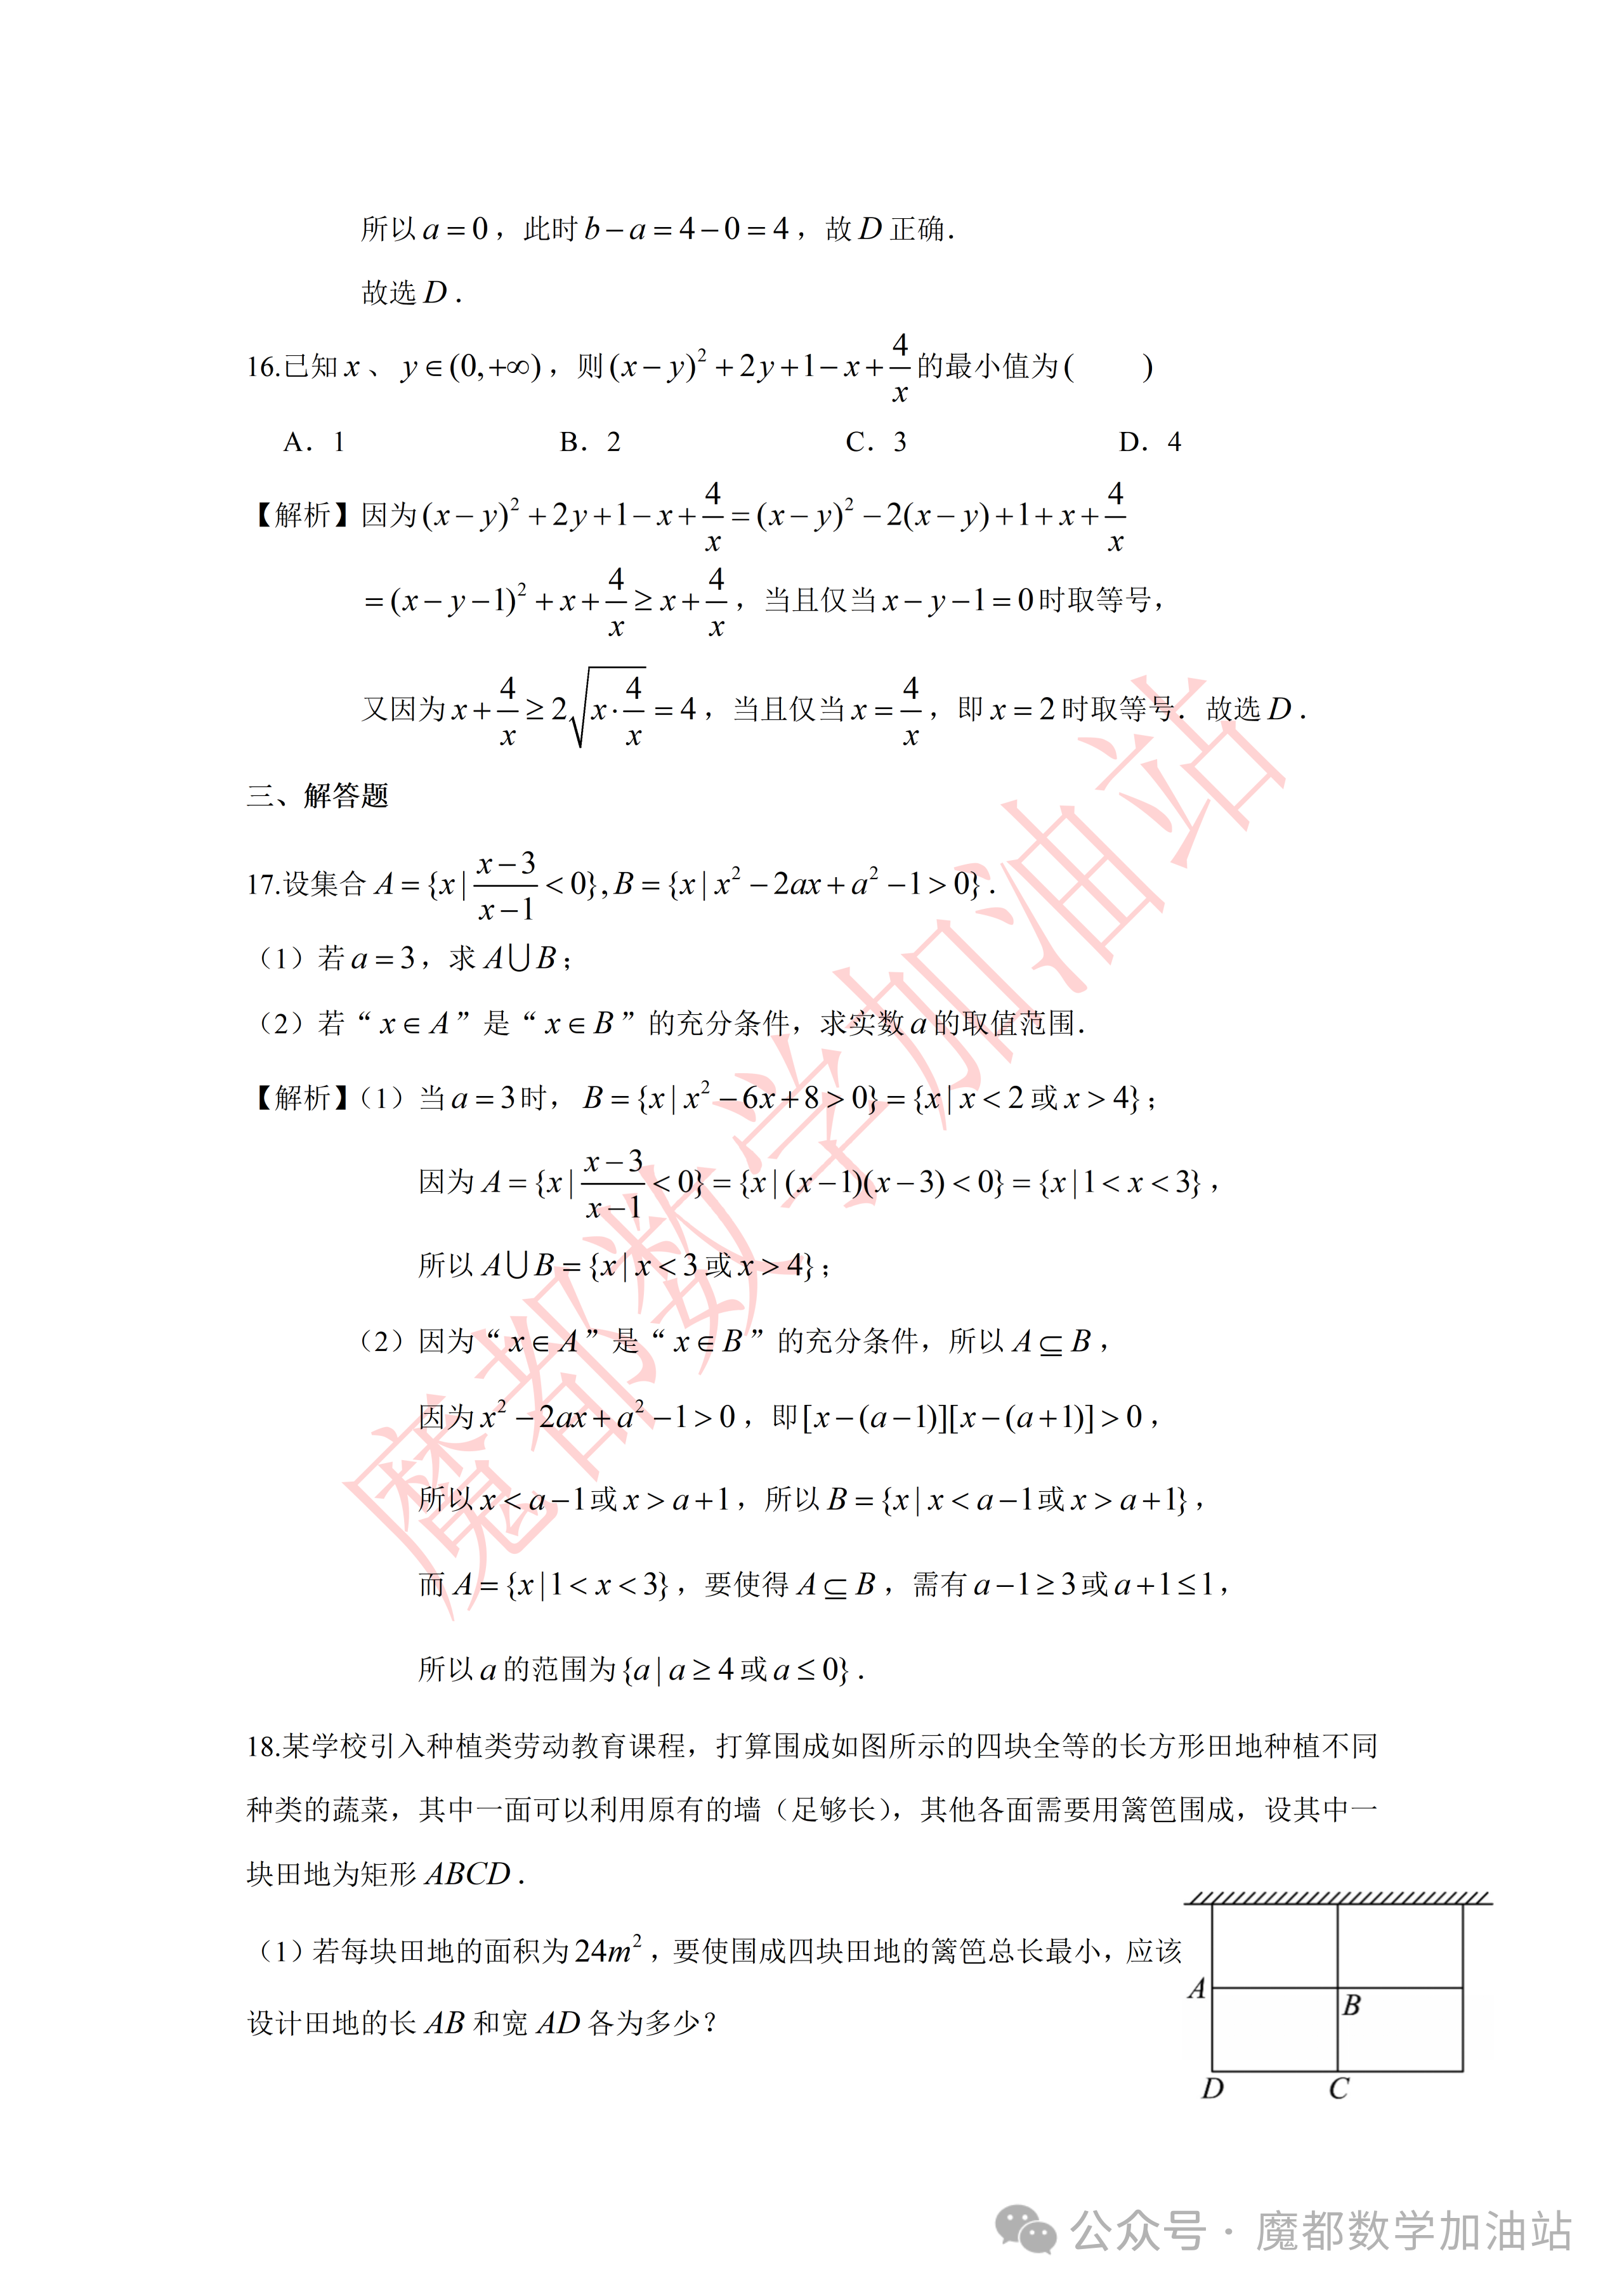
\includegraphics[width=.33\linewidth,trim=1866bp 220bp 210bp 2960bp,clip]{../原图/高一46_交附闵行_国庆作业3/06.png}
\end{center}

\begin{enumerate}[label=(\arabic*)]
\item 若每块田地的面积为 $24\,\text{m}^2$，要使围成四块田地的篱笆总长最小，应该设计田地的长 $AB$ 和宽 $AD$ 各为多少？
\item 现有 $40\,\text{m}$ 长的篱笆，要使每块田地的面积最大，应该设计田地的长 $AB$ 和宽 $AD$ 各为多少？
\end{enumerate}

\ifanswer
\solbegin
\stepm{(1)}{设 $AB$ 长为 $x\,\text{m}$，$AD$ 宽为 $y\,\text{m}$，由题意得 $xy=24$，篱笆总长为 $4x+6y$，}
\step{$4x+6y\geqslant2\sqrt{4x\cdot6y}=2\sqrt{24xy}=48$，}
\step{当且仅当 $4x=6y$ 时取等号，解得 $x=6$，$y=4$，}
\step{所以田地的长 $AB$ 为 $6\,\text{m}$，宽 $AD$ 为 $4\,\text{m}$.}
\stepm{(2)}{设 $AB$ 长为 $a\,\text{m}$，$AD$ 宽为 $b\,\text{m}$，由篱笆总长 $4a+6b=40$，即 $2a+3b=20$，}
\step{将 $a=\dfrac{20-3b}{2}$ 代入每块田地面积 $ab$，得 $ab=\dfrac12b(20-3b)=-\dfrac32b^2+10b$，}
\step{当 $b=\dfrac{10}{3}$ 时，$ab$ 最大，此时 $a=5$，}
\step{所以田地的长 $AB$ 为 $5\,\text{m}$，宽 $AD$ 为 $\dfrac{10}{3}\,\text{m}$.}
\solend
\fi

\ansspace[8]

\item 已知 $x_1$、$x_2$ 是一元二次方程 $4kx^2-4kx+k+1=0$ 的两个不等实数根.
\begin{enumerate}[label=(\arabic*)]
\item 若 $x_1$、$x_2$ 均为正根，求实数 $k$ 的取值范围；
\item 求使 $\dfrac{x_1}{x_2}+\dfrac{x_2}{x_1}-2$ 的值为整数 $k$ 的整数值.
\end{enumerate}

\ifanswer
\solbegin
\stepm{(1)}{由题意，$x_1$、$x_2$ 是方程 $4kx^2-4kx+k+1=0$ 的两个不等实数根，}
\step{故 $k\neq0$，$\Delta=(-4k)^2-16k(k+1)>0$，得 $-16k>0$，所以 $k<0$，}
\step{又 $x_1+x_2=1$，$x_1x_2=\dfrac{k+1}{4k}>0$，得 $k+1<0$，}
\step{所以 $k$ 的取值范围为 $(-\infty,-1)$.}
\stepm{(2)}{由题意，}
\step{$\dfrac{x_1}{x_2}+\dfrac{x_2}{x_1}-2
=\dfrac{x_1^2+x_2^2-2x_1x_2}{x_1x_2}
=\dfrac{(x_1+x_2)^2-4x_1x_2}{x_1x_2}$，}
\step{又 $x_1+x_2=1$，$x_1x_2=\dfrac{k+1}{4k}$，}
\step{则 $\dfrac{x_1}{x_2}+\dfrac{x_2}{x_1}-2=-\dfrac4{k+1}$，}
\step{由于 $-\dfrac4{k+1}$ 为整数，故 $k+1$ 只能取 $\pm1$、$\pm2$、$\pm4$，又 $k<-1$，}
\step{所以整数 $k$ 的值为 $-2$、$-3$、$-5$.}
\solend
\fi

\ansspace[8]

\item 已知 $a>0$，$b>0$，且 $2a+3b=3$.
\begin{enumerate}[label=(\arabic*)]
\item 求 $ab$ 的最大值；
\item 求 $a-\dfrac1{6b}$ 的最大值；
\item 求 $\dfrac2a+\dfrac3{b+1}$ 的最小值.
\end{enumerate}

\ifanswer
\solbegin
\stepm{(1)}{由 $2a+3b=3$，得 $3=2a+3b\geqslant2\sqrt{6ab}$，}
\step{所以 $ab\leqslant\dfrac38$，当且仅当 $2a=3b=\dfrac32$ 时取等号，}
\step{故 $ab$ 的最大值为 $\dfrac38$.}
\stepm{(2)}{由 $2a+3b=3$，得 $a=\dfrac32-\dfrac32b$，}
\step{则 $a-\dfrac1{6b}=\dfrac32-\dfrac32b-\dfrac1{6b}$，}
\step{由基本不等式，$\dfrac32b+\dfrac1{6b}\geqslant2\sqrt{\dfrac32b\cdot\dfrac1{6b}}=1$，}
\step{当且仅当 $\dfrac32b=\dfrac1{6b}$，即 $b=\dfrac13$、$a=1$ 时取等号，}
\step{所以 $a-\dfrac1{6b}$ 的最大值为 $\dfrac12$.}
\stepm{(3)}{由 $2a+3b=3$，得 $2a+3(b+1)=6$，}
\step{$\dfrac2a+\dfrac3{b+1}
=\dfrac16\left(2a+3(b+1)\right)\left(\dfrac2a+\dfrac3{b+1}\right)$}
\step{$=\dfrac16\left(13+\dfrac{6(b+1)}a+\dfrac{6a}{b+1}\right)
\geqslant\dfrac16\left(13+2\sqrt{\dfrac{6(b+1)}a\cdot\dfrac{6a}{b+1}}\right)=\dfrac{25}{6}$，}
\step{当且仅当 $a=b+1$，即 $a=\dfrac65$、$b=\dfrac15$ 时取等号，}
\step{所以 $\dfrac2a+\dfrac3{b+1}$ 的最小值为 $\dfrac{25}{6}$.}
\solend
\fi

\ansspace[8]

\item 已知 $U=\R$ 为全集，集合 $A=\{s^2+3t^2\mid s,t\in U\}$.
\begin{enumerate}[label=(\arabic*)]
\item 设 $U=\{1,3,5\}$，求集合 $A$ 的元素个数；
\item 设 $U=\Z$，证明：若 $x\in A$，则 $7x\in A$；
\item 设 $U=\R$，$x$、$y\in A$，且 $x=m^2+3n^2$，$y=p^2+3q^2$，若 $mp-3nq=\sqrt3$，求 $x+y+mq+np$ 的最小值.
\end{enumerate}

\ifanswer
\solbegin
\stepm{(1)}{当 $s=1$，$t=1$ 时，$s^2+3t^2=1+3=4$；}
\step{当 $s=1$，$t=3$ 时，$s^2+3t^2=1+27=28$；}
\step{当 $s=1$，$t=5$ 时，$s^2+3t^2=1+75=76$；}
\step{当 $s=3$，$t=1$ 时，$s^2+3t^2=9+3=12$；}
\step{当 $s=3$，$t=3$ 时，$s^2+3t^2=9+27=36$；}
\step{当 $s=3$，$t=5$ 时，$s^2+3t^2=9+75=84$；}
\step{当 $s=5$，$t=1$ 时，$s^2+3t^2=25+3=28$；}
\step{当 $s=5$，$t=3$ 时，$s^2+3t^2=25+27=52$；}
\step{当 $s=5$，$t=5$ 时，$s^2+3t^2=25+75=100$，}
\step{所以 $A=\{4,12,28,36,52,76,84,100\}$，有 $8$ 个元素.}
\stepm{(2)}{因为 $U=\Z$，$x\in A$，设 $x=s^2+3t^2$，}
\step{则 $7x=7(s^2+3t^2)=(2s+3t)^2+3(s-2t)^2\in A$，}
\step{所以 $7x\in A$.}
\stepm{(3)}{因为 $x=m^2+3n^2$，$y=p^2+3q^2$，}
\step{$xy=(m^2+3n^2)(p^2+3q^2)=3(mq+np)^2+(mp-3nq)^2$，}
\step{设 $mq+np=b$，则 $xy=3b^2+3$，所以 $y=\dfrac{3b^2+3}{x}$，}
\step{于是 $x+y+mq+np=x+\dfrac{3b^2+3}{x}+b\geqslant2\sqrt{3b^2+3}+b$，}
\step{设 $2\sqrt{3b^2+3}+b=t$，整理得 $11b^2+2bt+12-t^2=0$，}
\step{判别式法，$\Delta=4t^2-44(12-t^2)\geqslant0$，得 $t\geqslant\sqrt{11}$，}
\step{即 $(x+y+mq+np)_{\min}=\sqrt{11}$，所以 $x+y+mq+np$ 的最小值为 $\sqrt{11}$.}
\solend
\fi

\ansspace*[10]

\end{enumerate}

\end{document}
"
% 紧凑版：xelatex "\def\iscompact{1}% 高一46_交附闵行_国庆作业3.tex
%   —— 高一上数学“2026-2027 年交附闵行高一上国庆作业 3”（讲评版）
% 试卷版：xelatex 高一46_交附闵行_国庆作业3.tex
% 答案版：xelatex "\def\isanswer{1}\input{高一46_交附闵行_国庆作业3.tex}"
% 紧凑版：xelatex "\def\iscompact{1}\input{高一46_交附闵行_国庆作业3.tex}"
%
% 原始材料：微信公众号“魔都数学加油站”，作者破晓，2026-10-02 17:56 发布。
% 原文标题：“27学年高一46——2026-2027你那上海市交附闵行高一上国庆作业3”
% （公众号标题中的“你那”照录，系原文标题字样）；原文链接：
% http://mp.weixin.qq.com/s?__biz=Mzg4ODU1ODMxOQ==&mid=2247591657&idx=3&sn=a894d1a16611283a61b3eaba32a3f24c&chksm=cee83366c6a55381b370069f84ef63d20251f94608bb37cc4ec2d66227401bd147f4f6bd8256&scene=126&sessionid=1790935402&subscene=7&clicktime=1790937618&enterid=1790937618#rd
% 正文为 9 张 PNG 页，按页序读取原图；第 01、02、07 页 4762×6735，
% 第 03—06、08、09 页 2560×3620。卷面标题照原卷印作“2026-2027 年交附闵行高一上国庆作业 3”。
% 原文从第 3 题起，题号照原卷保留；正文为讲评版，答案、解析依原卷顺序录入。
% 水印及页脚公众号标识不录入。卷面插图直接裁取对应原图页，不另制图片文件。
%
% 与原卷的排版差异：
%   ① 原卷按“一、填空题”“二、选择题”“三、解答题”分节，本稿沿用原节与原题号，
%      只改排为全稿统一的大节样式；
%   ② 原卷答案与解析依页面位置分布，本稿按 common.sty 统一置于答案版；
%   ③ 原卷副标题未印，本稿按“知识模块”口径标作“集合与常用逻辑用语、不等式”。
%
% 原卷存疑一处（照抄未改，见第 12 题题干及解析处注释）：
%   第 12 题题干同时给出 x∈Z，却称不等式组有“50 个不等的实数解”；解析按整数根计数。
%   此处题干与解析的原文不一致，本稿均照录。
% 第 17 题曾疑似有常数项不一致：复核原图题干为 a^2-1，a=3 时常数项确为 8，
% 与解析相符；不将其记作原卷错误。
%
\documentclass[a4paper,11pt]{article}
\usepackage{common}

\begin{document}

\examtitlest[3]{2026--2027 年交附闵行高一上国庆作业 3}{集合与常用逻辑用语、不等式}

\bigsec{一、填空题}

\begin{enumerate}
\setcounter{enumi}{2}

\item 不等式 $\dfrac{x^2-10}{x+2}\geqslant1$ 的解集为\blankline[4.4em].

\ifanswer
\ans{$\{x\mid-3\leqslant x<-2\text{ 或 }x\geqslant4\}$}
\solbegin
\step{不等式 $\dfrac{x^2-10}{x+2}\geqslant1$，移项得 $\dfrac{x^2-10}{x+2}-1\geqslant0$，}
\step{通分得 $\dfrac{x^2-x-12}{x+2}\geqslant0$，即 $\dfrac{(x-4)(x+3)}{x+2}\geqslant0$，}
\step{解得 $-3\leqslant x<-2$ 或 $x\geqslant4$，}
\step{故不等式的解集为 $\{x\mid-3\leqslant x<-2\text{ 或 }x\geqslant4\}$.}
\solend
\fi

\item $|x-3|+|x-5|\geqslant2$，当等号成立时，$x$ 的范围是\blankline[4.4em].

\ifanswer
\ans{$[3,5]$}
\fi

\item 若直角三角形斜边长等于 $4\sqrt2\,\text{cm}$，则直角三角形面积的最大值为\blankline[4.4em].

\ifanswer
\solbegin
\step{设 $Rt\triangle ABC$ 中，$C=90^\circ$，则 $c=\sqrt{a^2+b^2}=4\sqrt2$，所以 $a^2+b^2=32$，}
\step{由基本不等式得 $a^2+b^2\geqslant2ab$，当且仅当 $a=b=4$ 时取等号，}
\step{所以 $\triangle ABC$ 的面积 $S=\dfrac12ab\leqslant8$，}
\step{当且仅当 $a=b=4$ 时，$\triangle ABC$ 的面积最大值为 $8$.}
\solend
\fi

\item 不等式 $(x-1)(2-x)>0$ 的解集为\blankline[4.4em].

\ifanswer
\solbegin
\step{$(x-1)(2-x)>0\Rightarrow(x-1)(x-2)<0$，}
\step{故不等式的解集为 $\{x\mid1<x<2\}$.}
\solend
\fi

\item 已知集合 $A=\{1,2\}$，$B=\{x\mid x^2-2mx+m=0\}$，$A\cup B=A$，则实数 $m$ 的取值范围为\blankline[4.4em].

\ifanswer
\solbegin
\step{因为 $A\cup B=A$，所以 $B\subseteq A$，}
\step{当 $B=\varnothing$ 时，$\Delta=(-2m)^2-4m<0$，解得 $0<m<1$，}
\step{当 $B$ 为单元素集时，$\Delta=0$，解得 $m=0$ 或 $m=1$，}
\step{当 $m=0$ 时，方程 $x^2=0$，解得 $x=0$，此时 $B=\{0\}$，不满足 $B\subseteq A$；}
\step{当 $m=1$ 时，方程 $x^2-2x+1=0$，解得 $x=1$，此时 $B=\{1\}$，满足 $B\subseteq A$；}
\step{当 $B=\{1,2\}$ 时，由韦达定理得 $1+2=2m$，$1\times2=m$，无解，}
\step{综上所述，实数 $m$ 的取值范围为 $\{m\mid0<m\leqslant1\}$.}
\solend
\fi

\item 设 $a$、$b$、$c\in\R^+$，若 $a+b+c=1$，则 $\dfrac1a+\dfrac1b+\dfrac1c\geqslant$\blankline[4.4em].

\ifanswer
\solbegin
\step{因为 $a$、$b$、$c\in\R^+$，且 $a+b+c=1$，}
\step{所以 $\dfrac1a+\dfrac1b+\dfrac1c=(a+b+c)\left(\dfrac1a+\dfrac1b+\dfrac1c\right)$}
\step{$=3+\dfrac ab+\dfrac ba+\dfrac ac+\dfrac ca+\dfrac bc+\dfrac cb$，}
\step{由基本不等式得 $\dfrac ab+\dfrac ba\geqslant2$，$\dfrac ac+\dfrac ca\geqslant2$，$\dfrac bc+\dfrac cb\geqslant2$，}
\step{所以 $\dfrac1a+\dfrac1b+\dfrac1c\geqslant9$，当且仅当 $a=b=c=\dfrac13$ 时取等号，}
\step{所以 $\dfrac1a+\dfrac1b+\dfrac1c$ 的最小值为 $9$.}
\solend
\fi

\item 已知 $-1\leqslant x+y\leqslant2$，$-2\leqslant x-y\leqslant1$，则 $x-2y$ 的范围为\blankline[4.4em].

\ifanswer
\solbegin
\step{设 $x-2y=m(x+y)+n(x-y)$，}
\step{则 $x-2y=(m+n)x+(m-n)y$，所以 $m+n=1$，$m-n=-2$，}
\step{解得 $m=-\dfrac12$，$n=\dfrac32$，}
\step{所以 $x-2y=-\dfrac12(x+y)+\dfrac32(x-y)$，}
\step{因为 $-1\leqslant x+y\leqslant2$，$-2\leqslant x-y\leqslant1$，}
\step{所以 $-4\leqslant x-2y\leqslant2$，即 $x-2y$ 的范围为 $[-4,2]$.}
\solend
\fi

\item 设集合 $A=\{1,2,m\}$，其中 $m$ 为实数，令 $B=\{a^2\mid a\in A\}$，$C=A\cup B$. 若 $C$ 中所有元素之和为 $6$，则 $C$ 中的所有元素之积为\blankline[4.4em].

\ifanswer
\solbegin
\step{因为 $A=\{1,2,m\}$，所以 $B=\{a^2\mid a\in A\}=\{1,4,m^2\}$，$m\neq1$，$m\neq2$，}
\step{又 $C=A\cup B$，所以 $1\in C$，$4\in C$，$m^2\in C$，}
\step{若 $m^2=1$，则 $m=-1$ 或 $m=1$（舍），当 $m=-1$ 时，$C=\{1,2,4,-1\}$，$C$ 中所有元素之和为 $6$，}
\step{此时 $C$ 中所有元素之积为 $-8$；}
\step{若 $m^2=2$，则 $m=-\sqrt2$ 或 $m=\sqrt2$，$C$ 中所有元素之和不符合题意；}
\step{若 $m^2=4$，则 $m=-2$ 或 $m=2$，此时 $C=\{1,2,4,-2\}$ 或 $C=\{1,2,4\}$，所有元素之和不符合题意；}
\step{若 $m^2\neq1$，$m^2\neq2$，$m^2\neq4$，则 $C=\{1,2,4,m,m^2\}$，}
\step{所以 $1+2+4+m+m^2=6$，即 $m^2+m+1=0$，无解，}
\step{综上所述，$C$ 中所有元素之积为 $-8$.}
\solend
\fi

\item 若对任意实数 $x>0$，$y>0$，不等式 $x+\sqrt{xy}\leqslant a(x+y)$ 恒成立，则实数 $a$ 的最小值为\blankline[4.4em].

\ifanswer
\solbegin
\step{由不等式 $x+\sqrt{xy}\leqslant a(x+y)$ 对任意实数 $x>0$，$y>0$ 恒成立，}
\step{得 $a\geqslant\dfrac{x+\sqrt{xy}}{x+y}$，}
\step{设 $\sqrt{\dfrac yx}=t>0$，则 $a\geqslant\dfrac{1+t}{1+t^2}$，}
\step{$\dfrac{1+t}{1+t^2}\leqslant\dfrac{\sqrt2+1}{2}$，当且仅当 $t=\sqrt2-1$ 时取等号，}
\step{所以实数 $a$ 的最小值为 $\dfrac{\sqrt2+1}{2}$.}
\solend
\fi

% 注：原卷题干给出 x∈Z，却写“实数解”；解析按整数解计数，题干与解析不一致，照录未改。
\item 若关于 $x$ 的不等式组
$\begin{cases}x^2-3mx\geqslant4m^2\\-20<x<120\end{cases}$（$x\in\Z,m>0$）恰有 $50$ 个不等的实数解，则 $m$ 的取值范围为\blankline[4.4em]（结果用区间表示）.

\ifanswer
\solbegin
\step{由 $x^2-3mx\geqslant4m^2$ 以及 $m>0$，解得 $x\leqslant-m$ 或 $x\geqslant4m$，}
\step{由原不等式组恰有 $50$ 个不等的实数解，可画出如下解集区间：}
\begin{center}
% 原图第 4 页数轴图直接裁取。
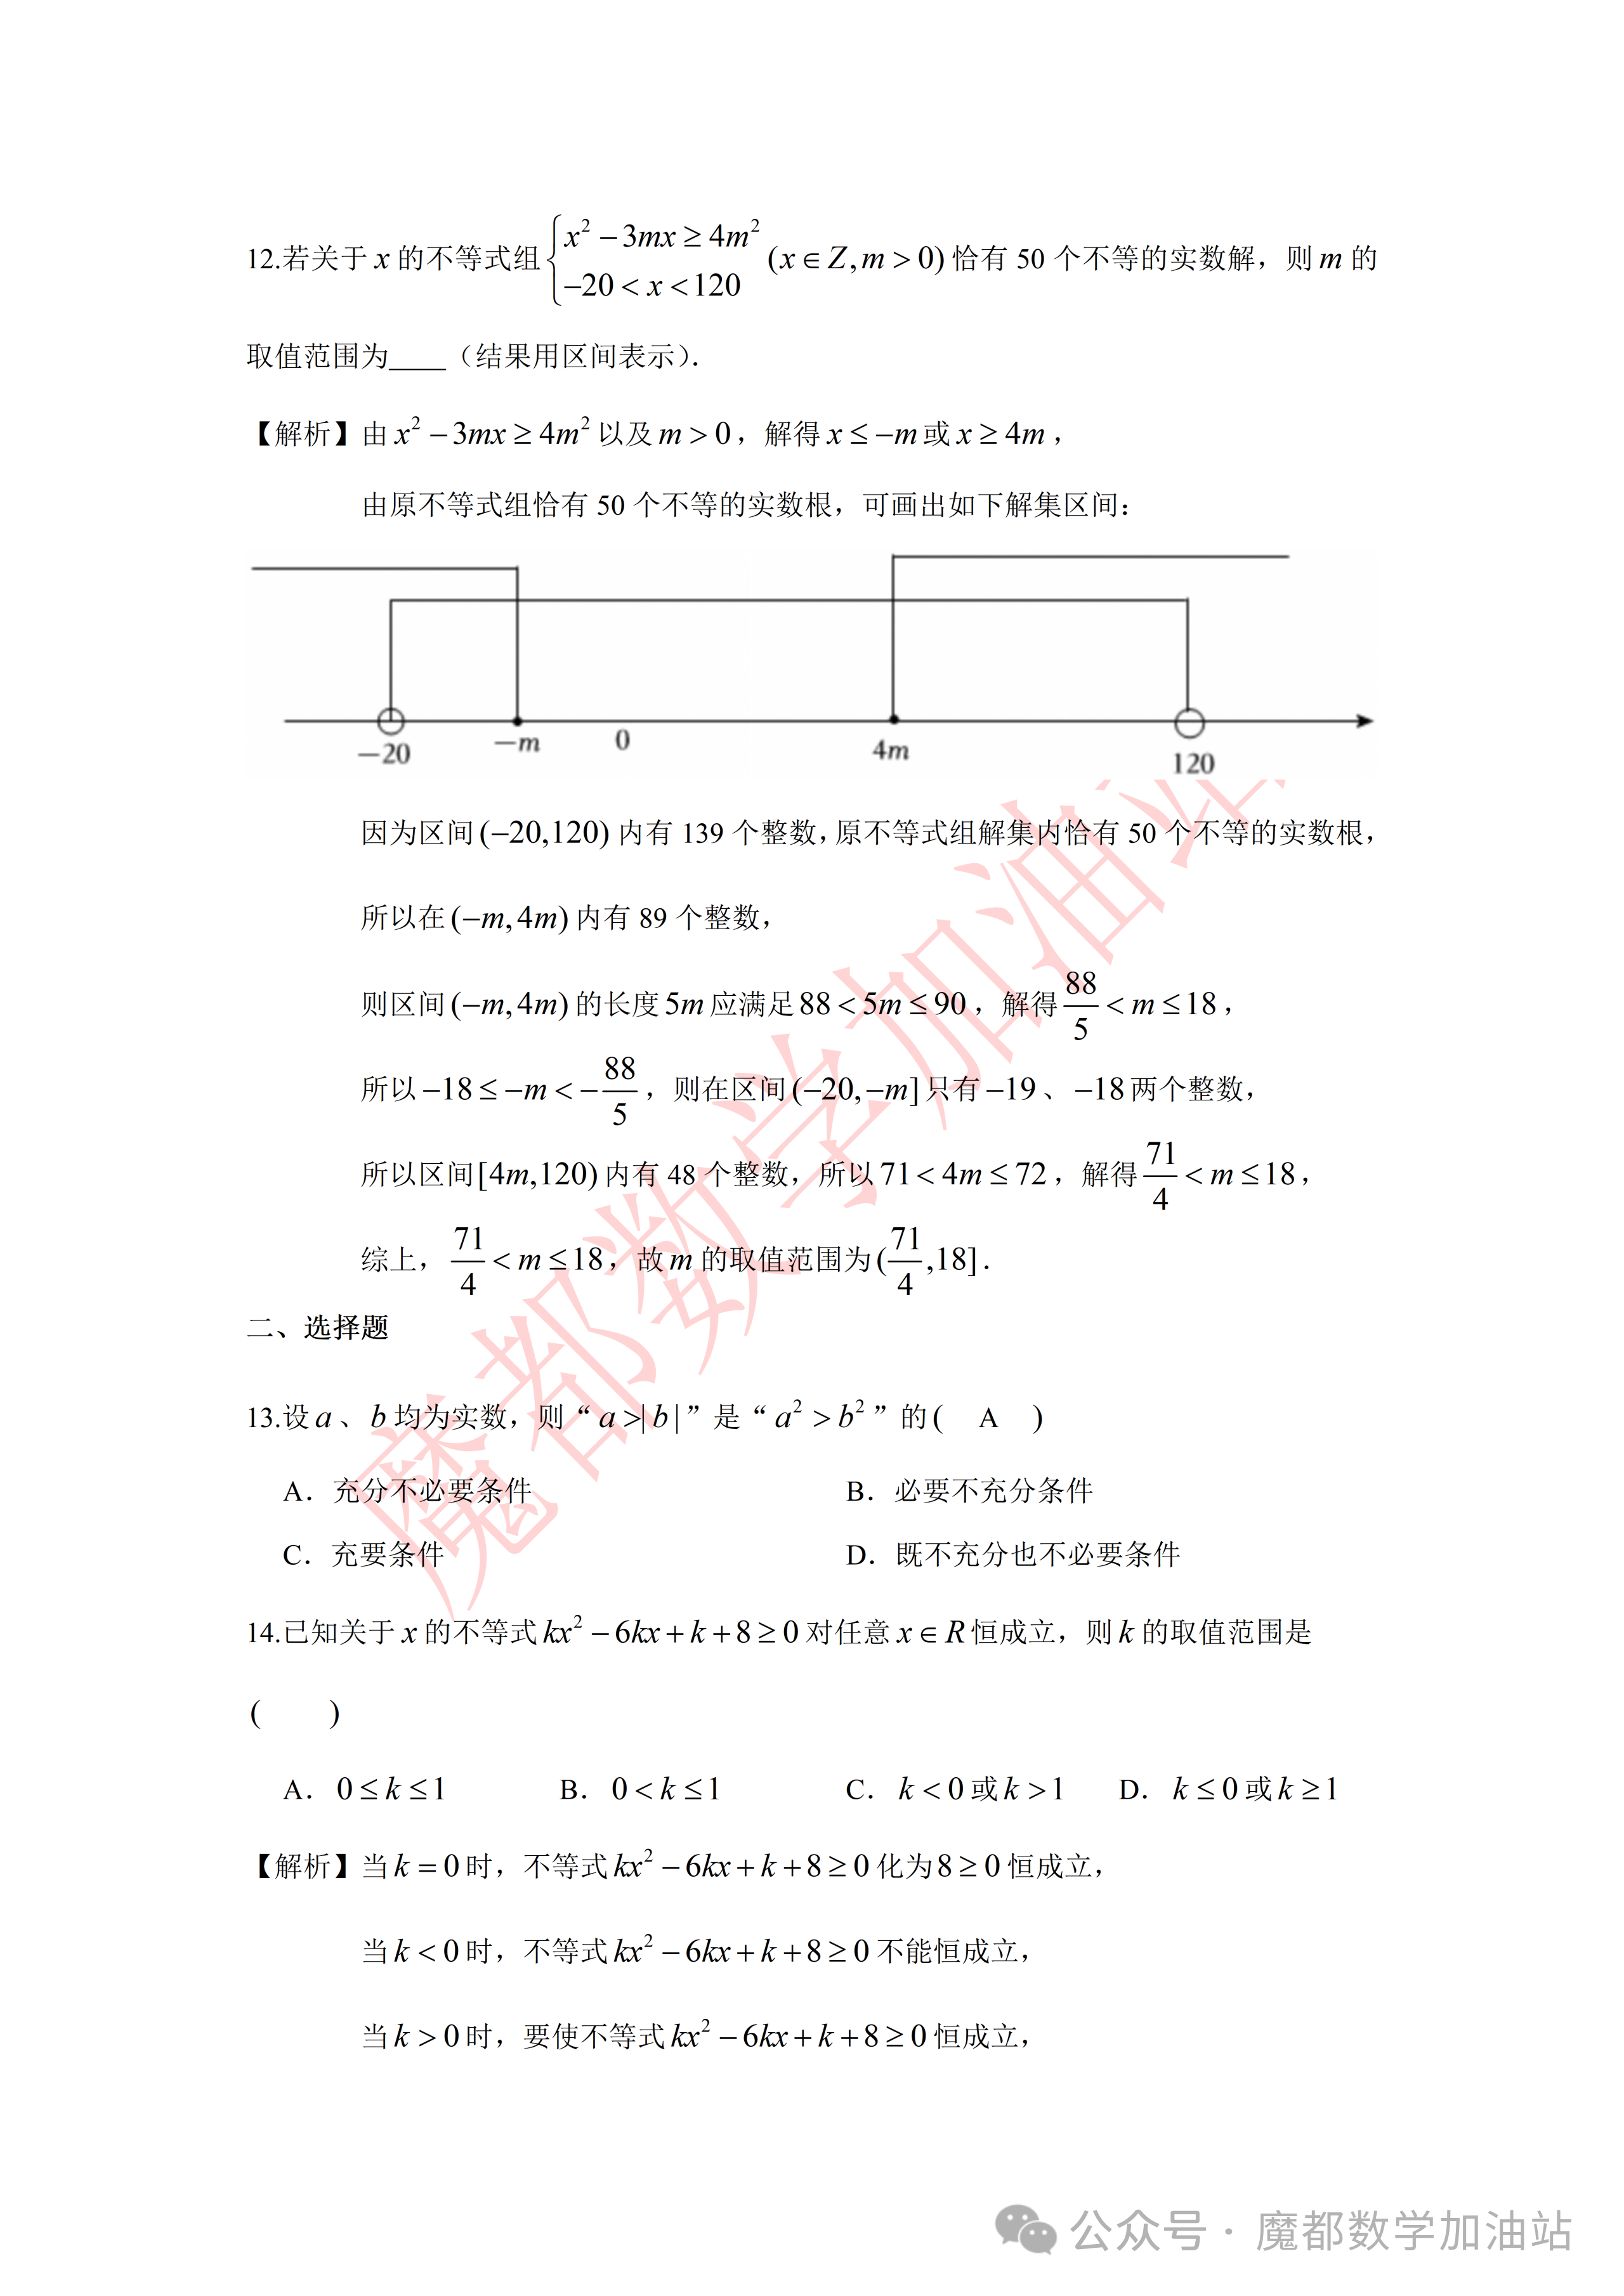
\includegraphics[width=.88\linewidth,trim=400bp 2410bp 320bp 860bp,clip]{../原图/高一46_交附闵行_国庆作业3/04.png}
\end{center}
\step{因为区间 $(-20,120)$ 内有 $139$ 个整数，原不等式组解集内有 $50$ 个不等的整数根，}
\step{所以在区间 $(-m,4m)$ 内有 $89$ 个整数，}
\step{则区间 $(-m,4m)$ 的长度 $5m$ 应满足 $88<5m\leqslant90$，解得 $\dfrac{88}{5}<m\leqslant18$，}
% 注：原卷题干称“实数解”，本行及后文按原卷解析照录为整数根计数。
\step{所以 $-18\leqslant-m<-\dfrac{88}{5}$，则在区间 $(-20,-m]$ 内有 $-19$、$-18$ 两个整数，}
\step{所以区间 $[4m,120)$ 内有 $48$ 个整数，}
\step{则 $71<4m\leqslant72$，解得 $\dfrac{71}{4}<m\leqslant18$，}
\step{综上，$\dfrac{71}{4}<m\leqslant18$，故 $m$ 的取值范围为 $\left(\dfrac{71}{4},18\right]$.}
\solend
\fi

\end{enumerate}

\bigsec{二、选择题}

\begin{enumerate}
\setcounter{enumi}{12}

\item 设 $a$、$b$ 均为实数，则“$a>|b|$”是“$a^2>b^2$”的\mbox{（\quad）}

\keepwithprev
A. 充分不必要条件\qquad B. 必要不充分条件

C. 充要条件\qquad\qquad D. 既不充分也不必要条件

\ans{$A$}

\item 已知关于 $x$ 的不等式 $kx^2-6kx+k+8\geqslant0$ 对任意 $x\in\R$ 恒成立，则 $k$ 的取值范围是\mbox{（\quad）}

\keepwithprev
A. $0\leqslant k\leqslant1$\qquad B. $0<k\leqslant1$

C. $k<0$ 或 $k>1$\qquad D. $k\leqslant0$ 或 $k\geqslant1$

\ans{$A$}

\ifanswer
\solbegin
\step{当 $k=0$ 时，不等式 $kx^2-6kx+k+8\geqslant0$ 化为 $8\geqslant0$ 恒成立，}
\step{当 $k<0$ 时，不等式 $kx^2-6kx+k+8\geqslant0$ 不能恒成立，}
\step{当 $k>0$ 时，要使不等式 $kx^2-6kx+k+8\geqslant0$ 恒成立，}
\step{需 $\Delta=36k^2-4(k^2+8k)\leqslant0$，解得 $0\leqslant k\leqslant1$，故选 $A$.}
\solend
\fi

\item 已知关于 $x$ 的不等式 $a\leqslant\dfrac34x^2-3x+4\leqslant b$，下列结论正确的是\mbox{（\quad）}

\keepwithprev
A. 当 $a<b<1$ 时，不等式 $a\leqslant\dfrac34x^2-3x+4\leqslant b$ 的解集非空

B. 当 $a=2$ 时，不等式 $a\leqslant\dfrac34x^2-3x+4\leqslant b$ 的解集可以为 $\{x\mid c\leqslant x\leqslant d\}$ 的形式

C. 不等式 $a\leqslant\dfrac34x^2-3x+4\leqslant b$ 的解集恰好为 $\{x\mid a\leqslant x\leqslant b\}$，那么 $b=\dfrac43$

D. 不等式 $a\leqslant\dfrac34x^2-3x+4\leqslant b$ 的解集恰好为 $\{x\mid a\leqslant x\leqslant b\}$，那么 $b-a=4$

\ans{$D$}

\ifanswer
\solbegin
\step{由 $\dfrac34x^2-3x+4\leqslant b$，得 $3x^2-12x+16-4b\leqslant0$，又 $b<1$，}
\step{所以 $\Delta=144-12(16-4b)=48(b-1)<0$，从而不等式无解，故 $A$ 错误；}
\step{在同一平面直角坐标系中作出函数 $y=\dfrac34x^2-3x+4=\dfrac34(x-2)^2+1$ 的图象及直线 $y=a$ 和 $y=b$，如图所示.}
\begin{center}
% 原图第 5 页解析配图直接裁取。
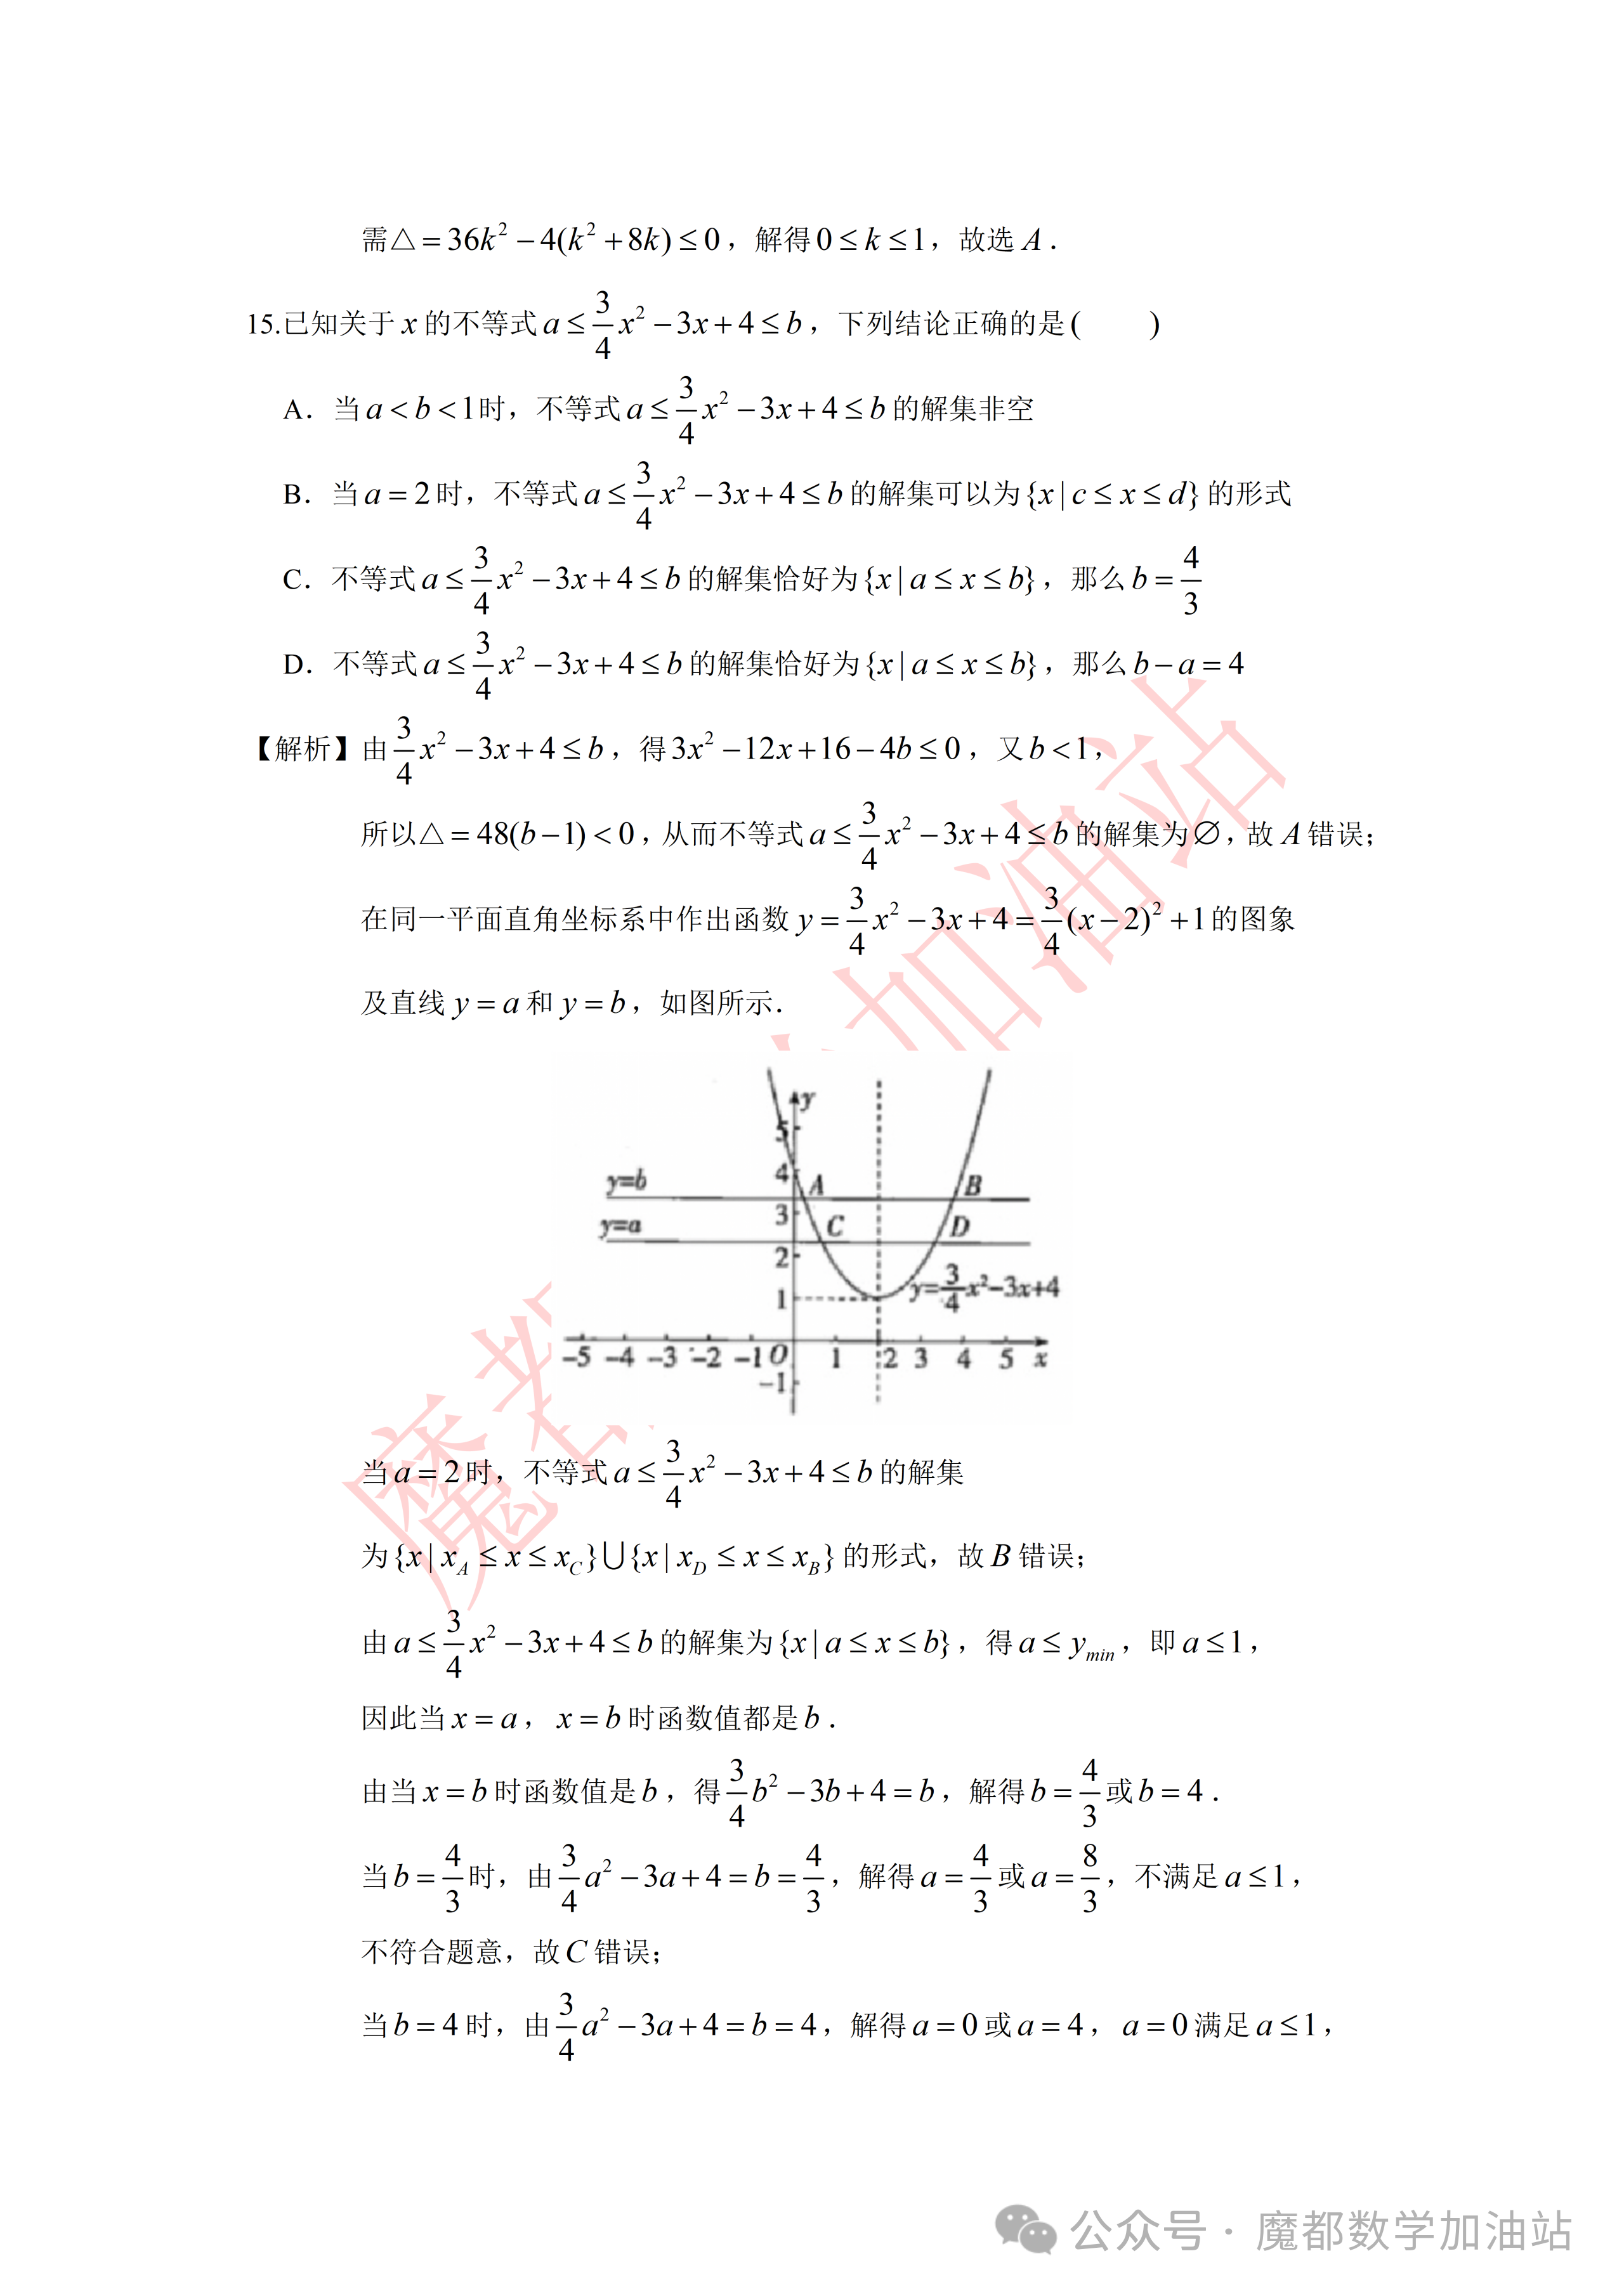
\includegraphics[width=.55\linewidth,trim=900bp 1400bp 760bp 1680bp,clip]{../原图/高一46_交附闵行_国庆作业3/05.png}
\end{center}
\step{当 $a=2$ 时，不等式 $a\leqslant\dfrac34x^2-3x+4\leqslant b$ 的解集为
$\{x\mid x_A\leqslant x\leqslant x_C\}\cup\{x\mid x_D\leqslant x\leqslant x_B\}$ 的形式，故 $B$ 错误；}
\step{由 $a\leqslant\dfrac34x^2-3x+4\leqslant b$ 的解集恰好为 $\{x\mid a\leqslant x\leqslant b\}$ 的形式，得 $a\leqslant y_{\min}$，即 $a\leqslant1$，}
\step{因为当 $x=a$、$x=b$ 时函数值都是 $b$，当 $x=a$ 时，$\dfrac34a^2-3a+4=b$；当 $x=b$ 时，$\dfrac34b^2-3b+4=b$，}
\step{解得 $b=\dfrac43$ 或 $b=4$，}
\step{当 $b=\dfrac43$ 时，由 $\dfrac34a^2-3a+4=b$，解得 $a=\dfrac43$ 或 $a=\dfrac83$，不符合题意，故 $C$ 错误；}
\step{当 $b=4$ 时，由 $\dfrac34a^2-3a+4=b$，解得 $a=0$ 或 $a=4$，$a=0$ 满足 $a\leqslant1$，故 $D$ 正确；}
\step{故选 $D$.}
\solend
\fi

\item 已知 $x$、$y\in(0,+\infty)$，则 $(x-y)^2+2y+1-x+\dfrac4x$ 的最小值为\mbox{（\quad）}

\keepwithprev
A. $1$\qquad B. $2$\qquad C. $3$\qquad D. $4$

\ans{$D$}

\ifanswer
\solbegin
\step{因为 $(x-y)^2+2y+1-x+\dfrac4x=(x-y-1)^2+x+\dfrac4x$，}
\step{当且仅当 $x-y-1=0$，且 $x=\dfrac4x$ 时取等号，}
\step{又因为 $x+\dfrac4x\geqslant2\sqrt{x\cdot\dfrac4x}=4$，当且仅当 $x=2$ 时取等号，}
\step{故选 $D$.}
\solend
\fi

\end{enumerate}

\bigsec{三、解答题}

\begin{enumerate}
\setcounter{enumi}{16}

\item 设集合 $A=\left\{x\middle|\dfrac{x-3}{x-1}<0\right\}$，$B=\{x\mid x^2-2ax+a^2-1>0\}$.
\begin{enumerate}[label=(\arabic*)]
\item 若 $a=3$，求 $A\cup B$；
\item 若“$x\in A$”是“$x\in B$”的充分条件，求实数 $a$ 的取值范围.
\end{enumerate}

\ifanswer
\solbegin
% 注：原卷题干为 a^2-1，故 a=3 时常数项为 8；题干与本步一致。
\stepm{(1)}{当 $a=3$ 时，$B=\{x\mid x^2-6x+8>0\}=\{x\mid x<2\text{ 或 }x>4\}$；}
\step{因为 $A=\left\{x\middle|\dfrac{x-3}{x-1}<0\right\}=\{x\mid(x-1)(x-3)<0\}=\{x\mid1<x<3\}$，}
\step{所以 $A\cup B=\{x\mid x<2\text{ 或 }x>4\}\cup\{x\mid1<x<3\}
=\{x\mid x<3\text{ 或 }x>4\}$.}
\stepm{(2)}{因为“$x\in A$”是“$x\in B$”的充分条件，所以 $A\subseteq B$，}
\step{因 $A=\left\{x\middle|\dfrac{x-3}{x-1}<0\right\}
=\{x\mid(x-1)(x-3)<0\}=\{x\mid1<x<3\}$，}
\step{所以 $A\subseteq B=\{x\mid x<a-1\text{ 或 }x>a+1\}$，}
\step{要使 $A\subseteq B$，需有 $a-1\geqslant3$ 或 $a+1\leqslant1$，}
\step{所以 $a\geqslant4$ 或 $a\leqslant0$，故 $a$ 的取值范围为 $\{a\mid a\geqslant4\text{ 或 }a\leqslant0\}$.}
\solend
\fi

\ansspace[6]

\item 某学校引入种植类劳动教育课程，打算围成如图所示的四块全等的长方形田地种植不同种类的蔬菜，其中一面可以利用原有的墙（足够长），其他各面需要用篱笆围成，设其中一块田地为矩形 $ABCD$.

\begin{center}
% 原图第 6 页配图直接裁取。
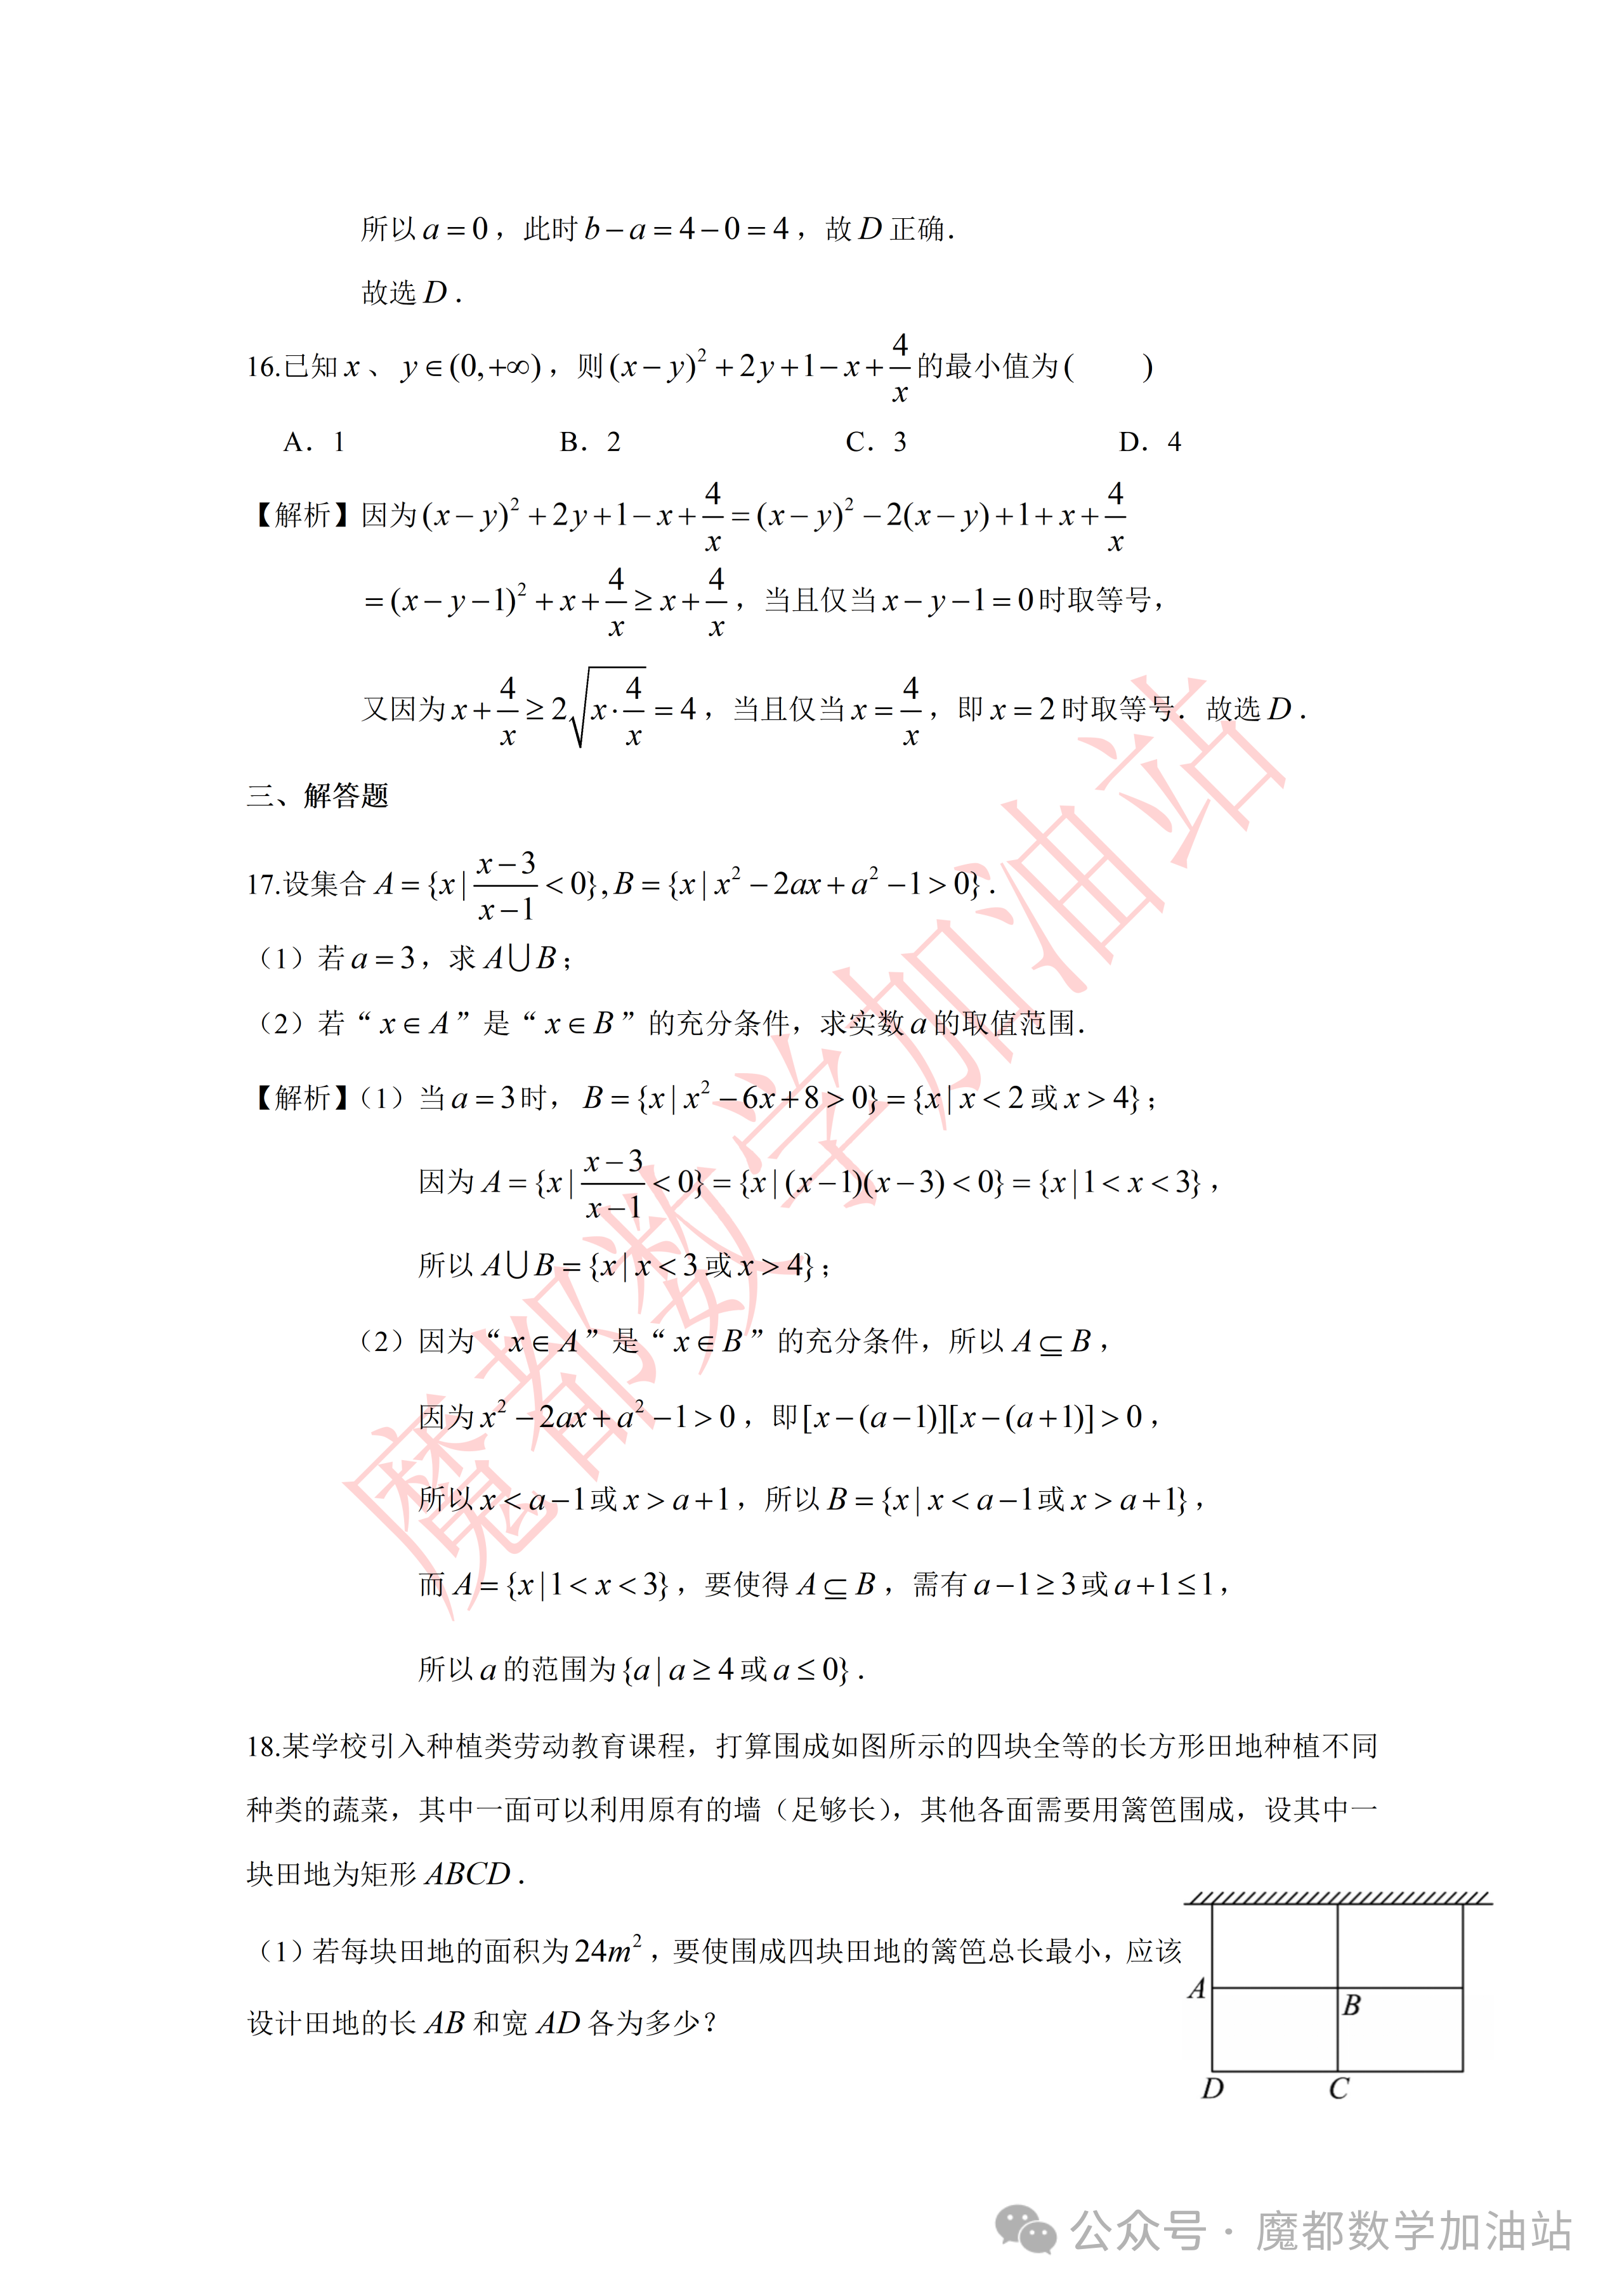
\includegraphics[width=.33\linewidth,trim=1866bp 220bp 210bp 2960bp,clip]{../原图/高一46_交附闵行_国庆作业3/06.png}
\end{center}

\begin{enumerate}[label=(\arabic*)]
\item 若每块田地的面积为 $24\,\text{m}^2$，要使围成四块田地的篱笆总长最小，应该设计田地的长 $AB$ 和宽 $AD$ 各为多少？
\item 现有 $40\,\text{m}$ 长的篱笆，要使每块田地的面积最大，应该设计田地的长 $AB$ 和宽 $AD$ 各为多少？
\end{enumerate}

\ifanswer
\solbegin
\stepm{(1)}{设 $AB$ 长为 $x\,\text{m}$，$AD$ 宽为 $y\,\text{m}$，由题意得 $xy=24$，篱笆总长为 $4x+6y$，}
\step{$4x+6y\geqslant2\sqrt{4x\cdot6y}=2\sqrt{24xy}=48$，}
\step{当且仅当 $4x=6y$ 时取等号，解得 $x=6$，$y=4$，}
\step{所以田地的长 $AB$ 为 $6\,\text{m}$，宽 $AD$ 为 $4\,\text{m}$.}
\stepm{(2)}{设 $AB$ 长为 $a\,\text{m}$，$AD$ 宽为 $b\,\text{m}$，由篱笆总长 $4a+6b=40$，即 $2a+3b=20$，}
\step{将 $a=\dfrac{20-3b}{2}$ 代入每块田地面积 $ab$，得 $ab=\dfrac12b(20-3b)=-\dfrac32b^2+10b$，}
\step{当 $b=\dfrac{10}{3}$ 时，$ab$ 最大，此时 $a=5$，}
\step{所以田地的长 $AB$ 为 $5\,\text{m}$，宽 $AD$ 为 $\dfrac{10}{3}\,\text{m}$.}
\solend
\fi

\ansspace[8]

\item 已知 $x_1$、$x_2$ 是一元二次方程 $4kx^2-4kx+k+1=0$ 的两个不等实数根.
\begin{enumerate}[label=(\arabic*)]
\item 若 $x_1$、$x_2$ 均为正根，求实数 $k$ 的取值范围；
\item 求使 $\dfrac{x_1}{x_2}+\dfrac{x_2}{x_1}-2$ 的值为整数 $k$ 的整数值.
\end{enumerate}

\ifanswer
\solbegin
\stepm{(1)}{由题意，$x_1$、$x_2$ 是方程 $4kx^2-4kx+k+1=0$ 的两个不等实数根，}
\step{故 $k\neq0$，$\Delta=(-4k)^2-16k(k+1)>0$，得 $-16k>0$，所以 $k<0$，}
\step{又 $x_1+x_2=1$，$x_1x_2=\dfrac{k+1}{4k}>0$，得 $k+1<0$，}
\step{所以 $k$ 的取值范围为 $(-\infty,-1)$.}
\stepm{(2)}{由题意，}
\step{$\dfrac{x_1}{x_2}+\dfrac{x_2}{x_1}-2
=\dfrac{x_1^2+x_2^2-2x_1x_2}{x_1x_2}
=\dfrac{(x_1+x_2)^2-4x_1x_2}{x_1x_2}$，}
\step{又 $x_1+x_2=1$，$x_1x_2=\dfrac{k+1}{4k}$，}
\step{则 $\dfrac{x_1}{x_2}+\dfrac{x_2}{x_1}-2=-\dfrac4{k+1}$，}
\step{由于 $-\dfrac4{k+1}$ 为整数，故 $k+1$ 只能取 $\pm1$、$\pm2$、$\pm4$，又 $k<-1$，}
\step{所以整数 $k$ 的值为 $-2$、$-3$、$-5$.}
\solend
\fi

\ansspace[8]

\item 已知 $a>0$，$b>0$，且 $2a+3b=3$.
\begin{enumerate}[label=(\arabic*)]
\item 求 $ab$ 的最大值；
\item 求 $a-\dfrac1{6b}$ 的最大值；
\item 求 $\dfrac2a+\dfrac3{b+1}$ 的最小值.
\end{enumerate}

\ifanswer
\solbegin
\stepm{(1)}{由 $2a+3b=3$，得 $3=2a+3b\geqslant2\sqrt{6ab}$，}
\step{所以 $ab\leqslant\dfrac38$，当且仅当 $2a=3b=\dfrac32$ 时取等号，}
\step{故 $ab$ 的最大值为 $\dfrac38$.}
\stepm{(2)}{由 $2a+3b=3$，得 $a=\dfrac32-\dfrac32b$，}
\step{则 $a-\dfrac1{6b}=\dfrac32-\dfrac32b-\dfrac1{6b}$，}
\step{由基本不等式，$\dfrac32b+\dfrac1{6b}\geqslant2\sqrt{\dfrac32b\cdot\dfrac1{6b}}=1$，}
\step{当且仅当 $\dfrac32b=\dfrac1{6b}$，即 $b=\dfrac13$、$a=1$ 时取等号，}
\step{所以 $a-\dfrac1{6b}$ 的最大值为 $\dfrac12$.}
\stepm{(3)}{由 $2a+3b=3$，得 $2a+3(b+1)=6$，}
\step{$\dfrac2a+\dfrac3{b+1}
=\dfrac16\left(2a+3(b+1)\right)\left(\dfrac2a+\dfrac3{b+1}\right)$}
\step{$=\dfrac16\left(13+\dfrac{6(b+1)}a+\dfrac{6a}{b+1}\right)
\geqslant\dfrac16\left(13+2\sqrt{\dfrac{6(b+1)}a\cdot\dfrac{6a}{b+1}}\right)=\dfrac{25}{6}$，}
\step{当且仅当 $a=b+1$，即 $a=\dfrac65$、$b=\dfrac15$ 时取等号，}
\step{所以 $\dfrac2a+\dfrac3{b+1}$ 的最小值为 $\dfrac{25}{6}$.}
\solend
\fi

\ansspace[8]

\item 已知 $U=\R$ 为全集，集合 $A=\{s^2+3t^2\mid s,t\in U\}$.
\begin{enumerate}[label=(\arabic*)]
\item 设 $U=\{1,3,5\}$，求集合 $A$ 的元素个数；
\item 设 $U=\Z$，证明：若 $x\in A$，则 $7x\in A$；
\item 设 $U=\R$，$x$、$y\in A$，且 $x=m^2+3n^2$，$y=p^2+3q^2$，若 $mp-3nq=\sqrt3$，求 $x+y+mq+np$ 的最小值.
\end{enumerate}

\ifanswer
\solbegin
\stepm{(1)}{当 $s=1$，$t=1$ 时，$s^2+3t^2=1+3=4$；}
\step{当 $s=1$，$t=3$ 时，$s^2+3t^2=1+27=28$；}
\step{当 $s=1$，$t=5$ 时，$s^2+3t^2=1+75=76$；}
\step{当 $s=3$，$t=1$ 时，$s^2+3t^2=9+3=12$；}
\step{当 $s=3$，$t=3$ 时，$s^2+3t^2=9+27=36$；}
\step{当 $s=3$，$t=5$ 时，$s^2+3t^2=9+75=84$；}
\step{当 $s=5$，$t=1$ 时，$s^2+3t^2=25+3=28$；}
\step{当 $s=5$，$t=3$ 时，$s^2+3t^2=25+27=52$；}
\step{当 $s=5$，$t=5$ 时，$s^2+3t^2=25+75=100$，}
\step{所以 $A=\{4,12,28,36,52,76,84,100\}$，有 $8$ 个元素.}
\stepm{(2)}{因为 $U=\Z$，$x\in A$，设 $x=s^2+3t^2$，}
\step{则 $7x=7(s^2+3t^2)=(2s+3t)^2+3(s-2t)^2\in A$，}
\step{所以 $7x\in A$.}
\stepm{(3)}{因为 $x=m^2+3n^2$，$y=p^2+3q^2$，}
\step{$xy=(m^2+3n^2)(p^2+3q^2)=3(mq+np)^2+(mp-3nq)^2$，}
\step{设 $mq+np=b$，则 $xy=3b^2+3$，所以 $y=\dfrac{3b^2+3}{x}$，}
\step{于是 $x+y+mq+np=x+\dfrac{3b^2+3}{x}+b\geqslant2\sqrt{3b^2+3}+b$，}
\step{设 $2\sqrt{3b^2+3}+b=t$，整理得 $11b^2+2bt+12-t^2=0$，}
\step{判别式法，$\Delta=4t^2-44(12-t^2)\geqslant0$，得 $t\geqslant\sqrt{11}$，}
\step{即 $(x+y+mq+np)_{\min}=\sqrt{11}$，所以 $x+y+mq+np$ 的最小值为 $\sqrt{11}$.}
\solend
\fi

\ansspace*[10]

\end{enumerate}

\end{document}
"
%
% 原始材料：微信公众号“魔都数学加油站”，作者破晓，2026-10-02 17:56 发布。
% 原文标题：“27学年高一46——2026-2027你那上海市交附闵行高一上国庆作业3”
% （公众号标题中的“你那”照录，系原文标题字样）；原文链接：
% http://mp.weixin.qq.com/s?__biz=Mzg4ODU1ODMxOQ==&mid=2247591657&idx=3&sn=a894d1a16611283a61b3eaba32a3f24c&chksm=cee83366c6a55381b370069f84ef63d20251f94608bb37cc4ec2d66227401bd147f4f6bd8256&scene=126&sessionid=1790935402&subscene=7&clicktime=1790937618&enterid=1790937618#rd
% 正文为 9 张 PNG 页，按页序读取原图；第 01、02、07 页 4762×6735，
% 第 03—06、08、09 页 2560×3620。卷面标题照原卷印作“2026-2027 年交附闵行高一上国庆作业 3”。
% 原文从第 3 题起，题号照原卷保留；正文为讲评版，答案、解析依原卷顺序录入。
% 水印及页脚公众号标识不录入。卷面插图直接裁取对应原图页，不另制图片文件。
%
% 与原卷的排版差异：
%   ① 原卷按“一、填空题”“二、选择题”“三、解答题”分节，本稿沿用原节与原题号，
%      只改排为全稿统一的大节样式；
%   ② 原卷答案与解析依页面位置分布，本稿按 common.sty 统一置于答案版；
%   ③ 原卷副标题未印，本稿按“知识模块”口径标作“集合与常用逻辑用语、不等式”。
%
% 原卷存疑一处（照抄未改，见第 12 题题干及解析处注释）：
%   第 12 题题干同时给出 x∈Z，却称不等式组有“50 个不等的实数解”；解析按整数根计数。
%   此处题干与解析的原文不一致，本稿均照录。
% 第 17 题曾疑似有常数项不一致：复核原图题干为 a^2-1，a=3 时常数项确为 8，
% 与解析相符；不将其记作原卷错误。
%
\documentclass[a4paper,11pt]{article}
\usepackage{common}

\begin{document}

\examtitlest[3]{2026--2027 年交附闵行高一上国庆作业 3}{集合与常用逻辑用语、不等式}

\bigsec{一、填空题}

\begin{enumerate}
\setcounter{enumi}{2}

\item 不等式 $\dfrac{x^2-10}{x+2}\geqslant1$ 的解集为\blankline[4.4em].

\ifanswer
\ans{$\{x\mid-3\leqslant x<-2\text{ 或 }x\geqslant4\}$}
\solbegin
\step{不等式 $\dfrac{x^2-10}{x+2}\geqslant1$，移项得 $\dfrac{x^2-10}{x+2}-1\geqslant0$，}
\step{通分得 $\dfrac{x^2-x-12}{x+2}\geqslant0$，即 $\dfrac{(x-4)(x+3)}{x+2}\geqslant0$，}
\step{解得 $-3\leqslant x<-2$ 或 $x\geqslant4$，}
\step{故不等式的解集为 $\{x\mid-3\leqslant x<-2\text{ 或 }x\geqslant4\}$.}
\solend
\fi

\item $|x-3|+|x-5|\geqslant2$，当等号成立时，$x$ 的范围是\blankline[4.4em].

\ifanswer
\ans{$[3,5]$}
\fi

\item 若直角三角形斜边长等于 $4\sqrt2\,\text{cm}$，则直角三角形面积的最大值为\blankline[4.4em].

\ifanswer
\solbegin
\step{设 $Rt\triangle ABC$ 中，$C=90^\circ$，则 $c=\sqrt{a^2+b^2}=4\sqrt2$，所以 $a^2+b^2=32$，}
\step{由基本不等式得 $a^2+b^2\geqslant2ab$，当且仅当 $a=b=4$ 时取等号，}
\step{所以 $\triangle ABC$ 的面积 $S=\dfrac12ab\leqslant8$，}
\step{当且仅当 $a=b=4$ 时，$\triangle ABC$ 的面积最大值为 $8$.}
\solend
\fi

\item 不等式 $(x-1)(2-x)>0$ 的解集为\blankline[4.4em].

\ifanswer
\solbegin
\step{$(x-1)(2-x)>0\Rightarrow(x-1)(x-2)<0$，}
\step{故不等式的解集为 $\{x\mid1<x<2\}$.}
\solend
\fi

\item 已知集合 $A=\{1,2\}$，$B=\{x\mid x^2-2mx+m=0\}$，$A\cup B=A$，则实数 $m$ 的取值范围为\blankline[4.4em].

\ifanswer
\solbegin
\step{因为 $A\cup B=A$，所以 $B\subseteq A$，}
\step{当 $B=\varnothing$ 时，$\Delta=(-2m)^2-4m<0$，解得 $0<m<1$，}
\step{当 $B$ 为单元素集时，$\Delta=0$，解得 $m=0$ 或 $m=1$，}
\step{当 $m=0$ 时，方程 $x^2=0$，解得 $x=0$，此时 $B=\{0\}$，不满足 $B\subseteq A$；}
\step{当 $m=1$ 时，方程 $x^2-2x+1=0$，解得 $x=1$，此时 $B=\{1\}$，满足 $B\subseteq A$；}
\step{当 $B=\{1,2\}$ 时，由韦达定理得 $1+2=2m$，$1\times2=m$，无解，}
\step{综上所述，实数 $m$ 的取值范围为 $\{m\mid0<m\leqslant1\}$.}
\solend
\fi

\item 设 $a$、$b$、$c\in\R^+$，若 $a+b+c=1$，则 $\dfrac1a+\dfrac1b+\dfrac1c\geqslant$\blankline[4.4em].

\ifanswer
\solbegin
\step{因为 $a$、$b$、$c\in\R^+$，且 $a+b+c=1$，}
\step{所以 $\dfrac1a+\dfrac1b+\dfrac1c=(a+b+c)\left(\dfrac1a+\dfrac1b+\dfrac1c\right)$}
\step{$=3+\dfrac ab+\dfrac ba+\dfrac ac+\dfrac ca+\dfrac bc+\dfrac cb$，}
\step{由基本不等式得 $\dfrac ab+\dfrac ba\geqslant2$，$\dfrac ac+\dfrac ca\geqslant2$，$\dfrac bc+\dfrac cb\geqslant2$，}
\step{所以 $\dfrac1a+\dfrac1b+\dfrac1c\geqslant9$，当且仅当 $a=b=c=\dfrac13$ 时取等号，}
\step{所以 $\dfrac1a+\dfrac1b+\dfrac1c$ 的最小值为 $9$.}
\solend
\fi

\item 已知 $-1\leqslant x+y\leqslant2$，$-2\leqslant x-y\leqslant1$，则 $x-2y$ 的范围为\blankline[4.4em].

\ifanswer
\solbegin
\step{设 $x-2y=m(x+y)+n(x-y)$，}
\step{则 $x-2y=(m+n)x+(m-n)y$，所以 $m+n=1$，$m-n=-2$，}
\step{解得 $m=-\dfrac12$，$n=\dfrac32$，}
\step{所以 $x-2y=-\dfrac12(x+y)+\dfrac32(x-y)$，}
\step{因为 $-1\leqslant x+y\leqslant2$，$-2\leqslant x-y\leqslant1$，}
\step{所以 $-4\leqslant x-2y\leqslant2$，即 $x-2y$ 的范围为 $[-4,2]$.}
\solend
\fi

\item 设集合 $A=\{1,2,m\}$，其中 $m$ 为实数，令 $B=\{a^2\mid a\in A\}$，$C=A\cup B$. 若 $C$ 中所有元素之和为 $6$，则 $C$ 中的所有元素之积为\blankline[4.4em].

\ifanswer
\solbegin
\step{因为 $A=\{1,2,m\}$，所以 $B=\{a^2\mid a\in A\}=\{1,4,m^2\}$，$m\neq1$，$m\neq2$，}
\step{又 $C=A\cup B$，所以 $1\in C$，$4\in C$，$m^2\in C$，}
\step{若 $m^2=1$，则 $m=-1$ 或 $m=1$（舍），当 $m=-1$ 时，$C=\{1,2,4,-1\}$，$C$ 中所有元素之和为 $6$，}
\step{此时 $C$ 中所有元素之积为 $-8$；}
\step{若 $m^2=2$，则 $m=-\sqrt2$ 或 $m=\sqrt2$，$C$ 中所有元素之和不符合题意；}
\step{若 $m^2=4$，则 $m=-2$ 或 $m=2$，此时 $C=\{1,2,4,-2\}$ 或 $C=\{1,2,4\}$，所有元素之和不符合题意；}
\step{若 $m^2\neq1$，$m^2\neq2$，$m^2\neq4$，则 $C=\{1,2,4,m,m^2\}$，}
\step{所以 $1+2+4+m+m^2=6$，即 $m^2+m+1=0$，无解，}
\step{综上所述，$C$ 中所有元素之积为 $-8$.}
\solend
\fi

\item 若对任意实数 $x>0$，$y>0$，不等式 $x+\sqrt{xy}\leqslant a(x+y)$ 恒成立，则实数 $a$ 的最小值为\blankline[4.4em].

\ifanswer
\solbegin
\step{由不等式 $x+\sqrt{xy}\leqslant a(x+y)$ 对任意实数 $x>0$，$y>0$ 恒成立，}
\step{得 $a\geqslant\dfrac{x+\sqrt{xy}}{x+y}$，}
\step{设 $\sqrt{\dfrac yx}=t>0$，则 $a\geqslant\dfrac{1+t}{1+t^2}$，}
\step{$\dfrac{1+t}{1+t^2}\leqslant\dfrac{\sqrt2+1}{2}$，当且仅当 $t=\sqrt2-1$ 时取等号，}
\step{所以实数 $a$ 的最小值为 $\dfrac{\sqrt2+1}{2}$.}
\solend
\fi

% 注：原卷题干给出 x∈Z，却写“实数解”；解析按整数解计数，题干与解析不一致，照录未改。
\item 若关于 $x$ 的不等式组
$\begin{cases}x^2-3mx\geqslant4m^2\\-20<x<120\end{cases}$（$x\in\Z,m>0$）恰有 $50$ 个不等的实数解，则 $m$ 的取值范围为\blankline[4.4em]（结果用区间表示）.

\ifanswer
\solbegin
\step{由 $x^2-3mx\geqslant4m^2$ 以及 $m>0$，解得 $x\leqslant-m$ 或 $x\geqslant4m$，}
\step{由原不等式组恰有 $50$ 个不等的实数解，可画出如下解集区间：}
\begin{center}
% 原图第 4 页数轴图直接裁取。
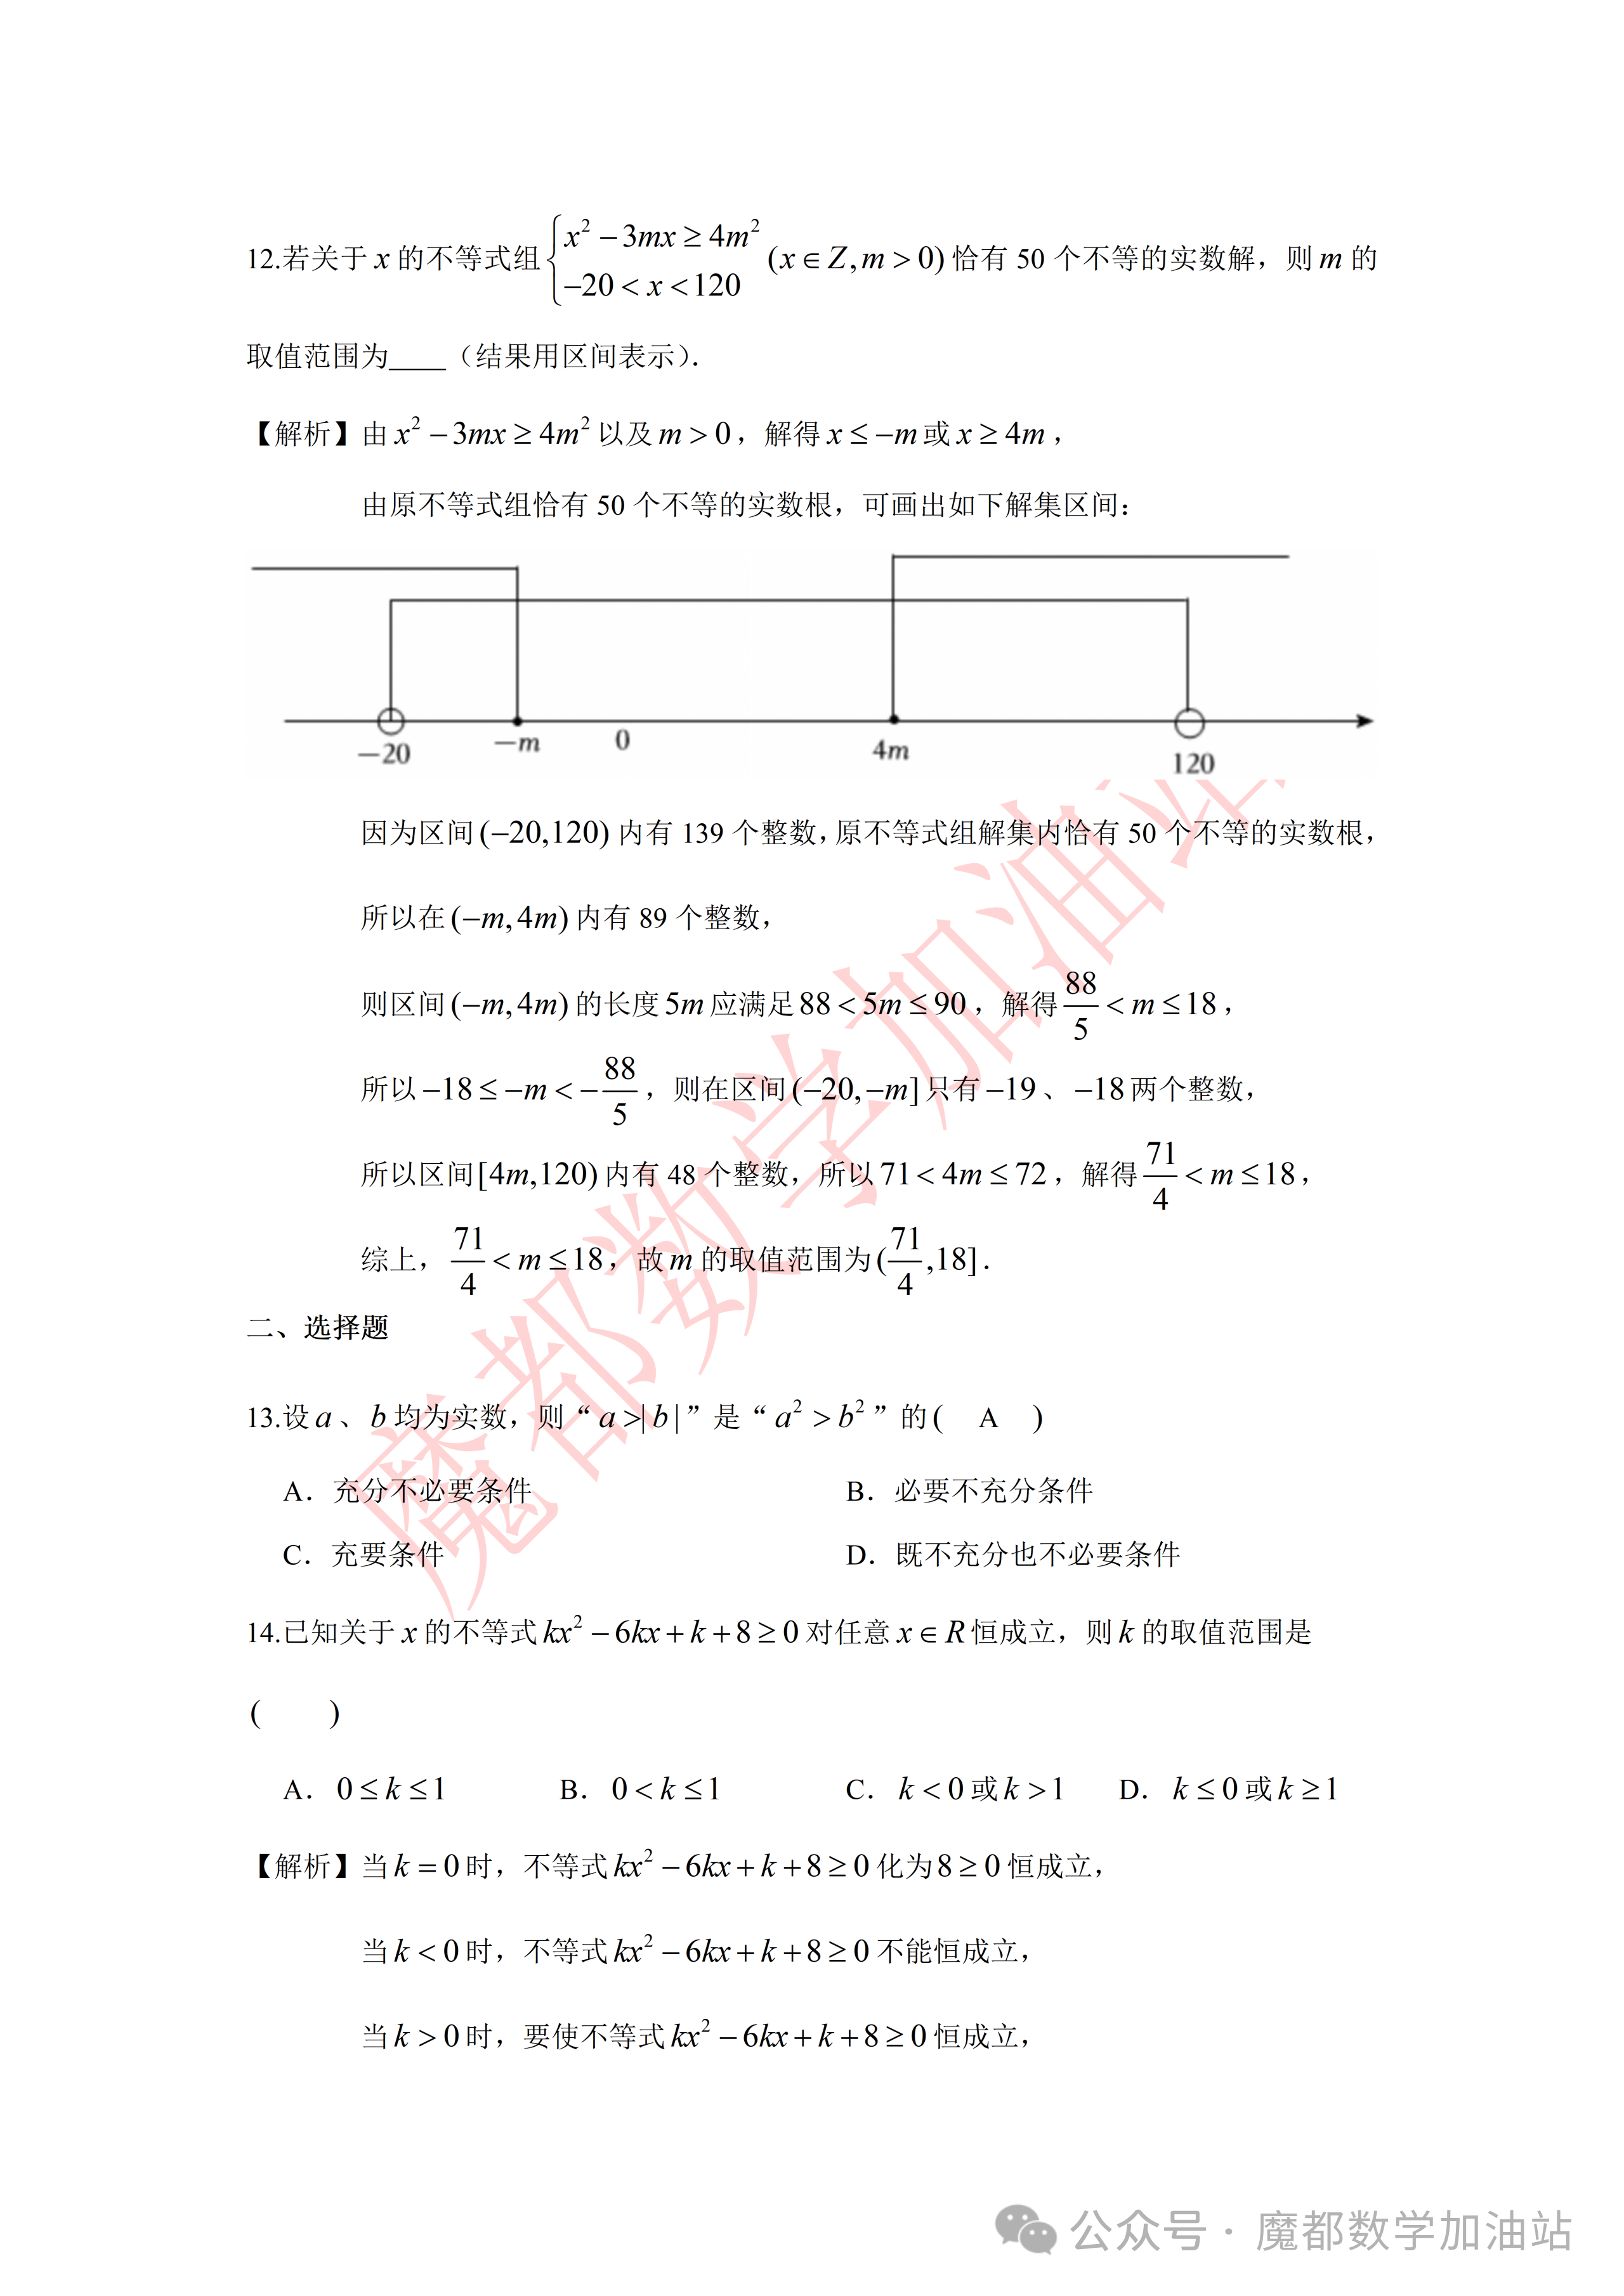
\includegraphics[width=.88\linewidth,trim=400bp 2410bp 320bp 860bp,clip]{../原图/高一46_交附闵行_国庆作业3/04.png}
\end{center}
\step{因为区间 $(-20,120)$ 内有 $139$ 个整数，原不等式组解集内有 $50$ 个不等的整数根，}
\step{所以在区间 $(-m,4m)$ 内有 $89$ 个整数，}
\step{则区间 $(-m,4m)$ 的长度 $5m$ 应满足 $88<5m\leqslant90$，解得 $\dfrac{88}{5}<m\leqslant18$，}
% 注：原卷题干称“实数解”，本行及后文按原卷解析照录为整数根计数。
\step{所以 $-18\leqslant-m<-\dfrac{88}{5}$，则在区间 $(-20,-m]$ 内有 $-19$、$-18$ 两个整数，}
\step{所以区间 $[4m,120)$ 内有 $48$ 个整数，}
\step{则 $71<4m\leqslant72$，解得 $\dfrac{71}{4}<m\leqslant18$，}
\step{综上，$\dfrac{71}{4}<m\leqslant18$，故 $m$ 的取值范围为 $\left(\dfrac{71}{4},18\right]$.}
\solend
\fi

\end{enumerate}

\bigsec{二、选择题}

\begin{enumerate}
\setcounter{enumi}{12}

\item 设 $a$、$b$ 均为实数，则“$a>|b|$”是“$a^2>b^2$”的\mbox{（\quad）}

\keepwithprev
A. 充分不必要条件\qquad B. 必要不充分条件

C. 充要条件\qquad\qquad D. 既不充分也不必要条件

\ans{$A$}

\item 已知关于 $x$ 的不等式 $kx^2-6kx+k+8\geqslant0$ 对任意 $x\in\R$ 恒成立，则 $k$ 的取值范围是\mbox{（\quad）}

\keepwithprev
A. $0\leqslant k\leqslant1$\qquad B. $0<k\leqslant1$

C. $k<0$ 或 $k>1$\qquad D. $k\leqslant0$ 或 $k\geqslant1$

\ans{$A$}

\ifanswer
\solbegin
\step{当 $k=0$ 时，不等式 $kx^2-6kx+k+8\geqslant0$ 化为 $8\geqslant0$ 恒成立，}
\step{当 $k<0$ 时，不等式 $kx^2-6kx+k+8\geqslant0$ 不能恒成立，}
\step{当 $k>0$ 时，要使不等式 $kx^2-6kx+k+8\geqslant0$ 恒成立，}
\step{需 $\Delta=36k^2-4(k^2+8k)\leqslant0$，解得 $0\leqslant k\leqslant1$，故选 $A$.}
\solend
\fi

\item 已知关于 $x$ 的不等式 $a\leqslant\dfrac34x^2-3x+4\leqslant b$，下列结论正确的是\mbox{（\quad）}

\keepwithprev
A. 当 $a<b<1$ 时，不等式 $a\leqslant\dfrac34x^2-3x+4\leqslant b$ 的解集非空

B. 当 $a=2$ 时，不等式 $a\leqslant\dfrac34x^2-3x+4\leqslant b$ 的解集可以为 $\{x\mid c\leqslant x\leqslant d\}$ 的形式

C. 不等式 $a\leqslant\dfrac34x^2-3x+4\leqslant b$ 的解集恰好为 $\{x\mid a\leqslant x\leqslant b\}$，那么 $b=\dfrac43$

D. 不等式 $a\leqslant\dfrac34x^2-3x+4\leqslant b$ 的解集恰好为 $\{x\mid a\leqslant x\leqslant b\}$，那么 $b-a=4$

\ans{$D$}

\ifanswer
\solbegin
\step{由 $\dfrac34x^2-3x+4\leqslant b$，得 $3x^2-12x+16-4b\leqslant0$，又 $b<1$，}
\step{所以 $\Delta=144-12(16-4b)=48(b-1)<0$，从而不等式无解，故 $A$ 错误；}
\step{在同一平面直角坐标系中作出函数 $y=\dfrac34x^2-3x+4=\dfrac34(x-2)^2+1$ 的图象及直线 $y=a$ 和 $y=b$，如图所示.}
\begin{center}
% 原图第 5 页解析配图直接裁取。
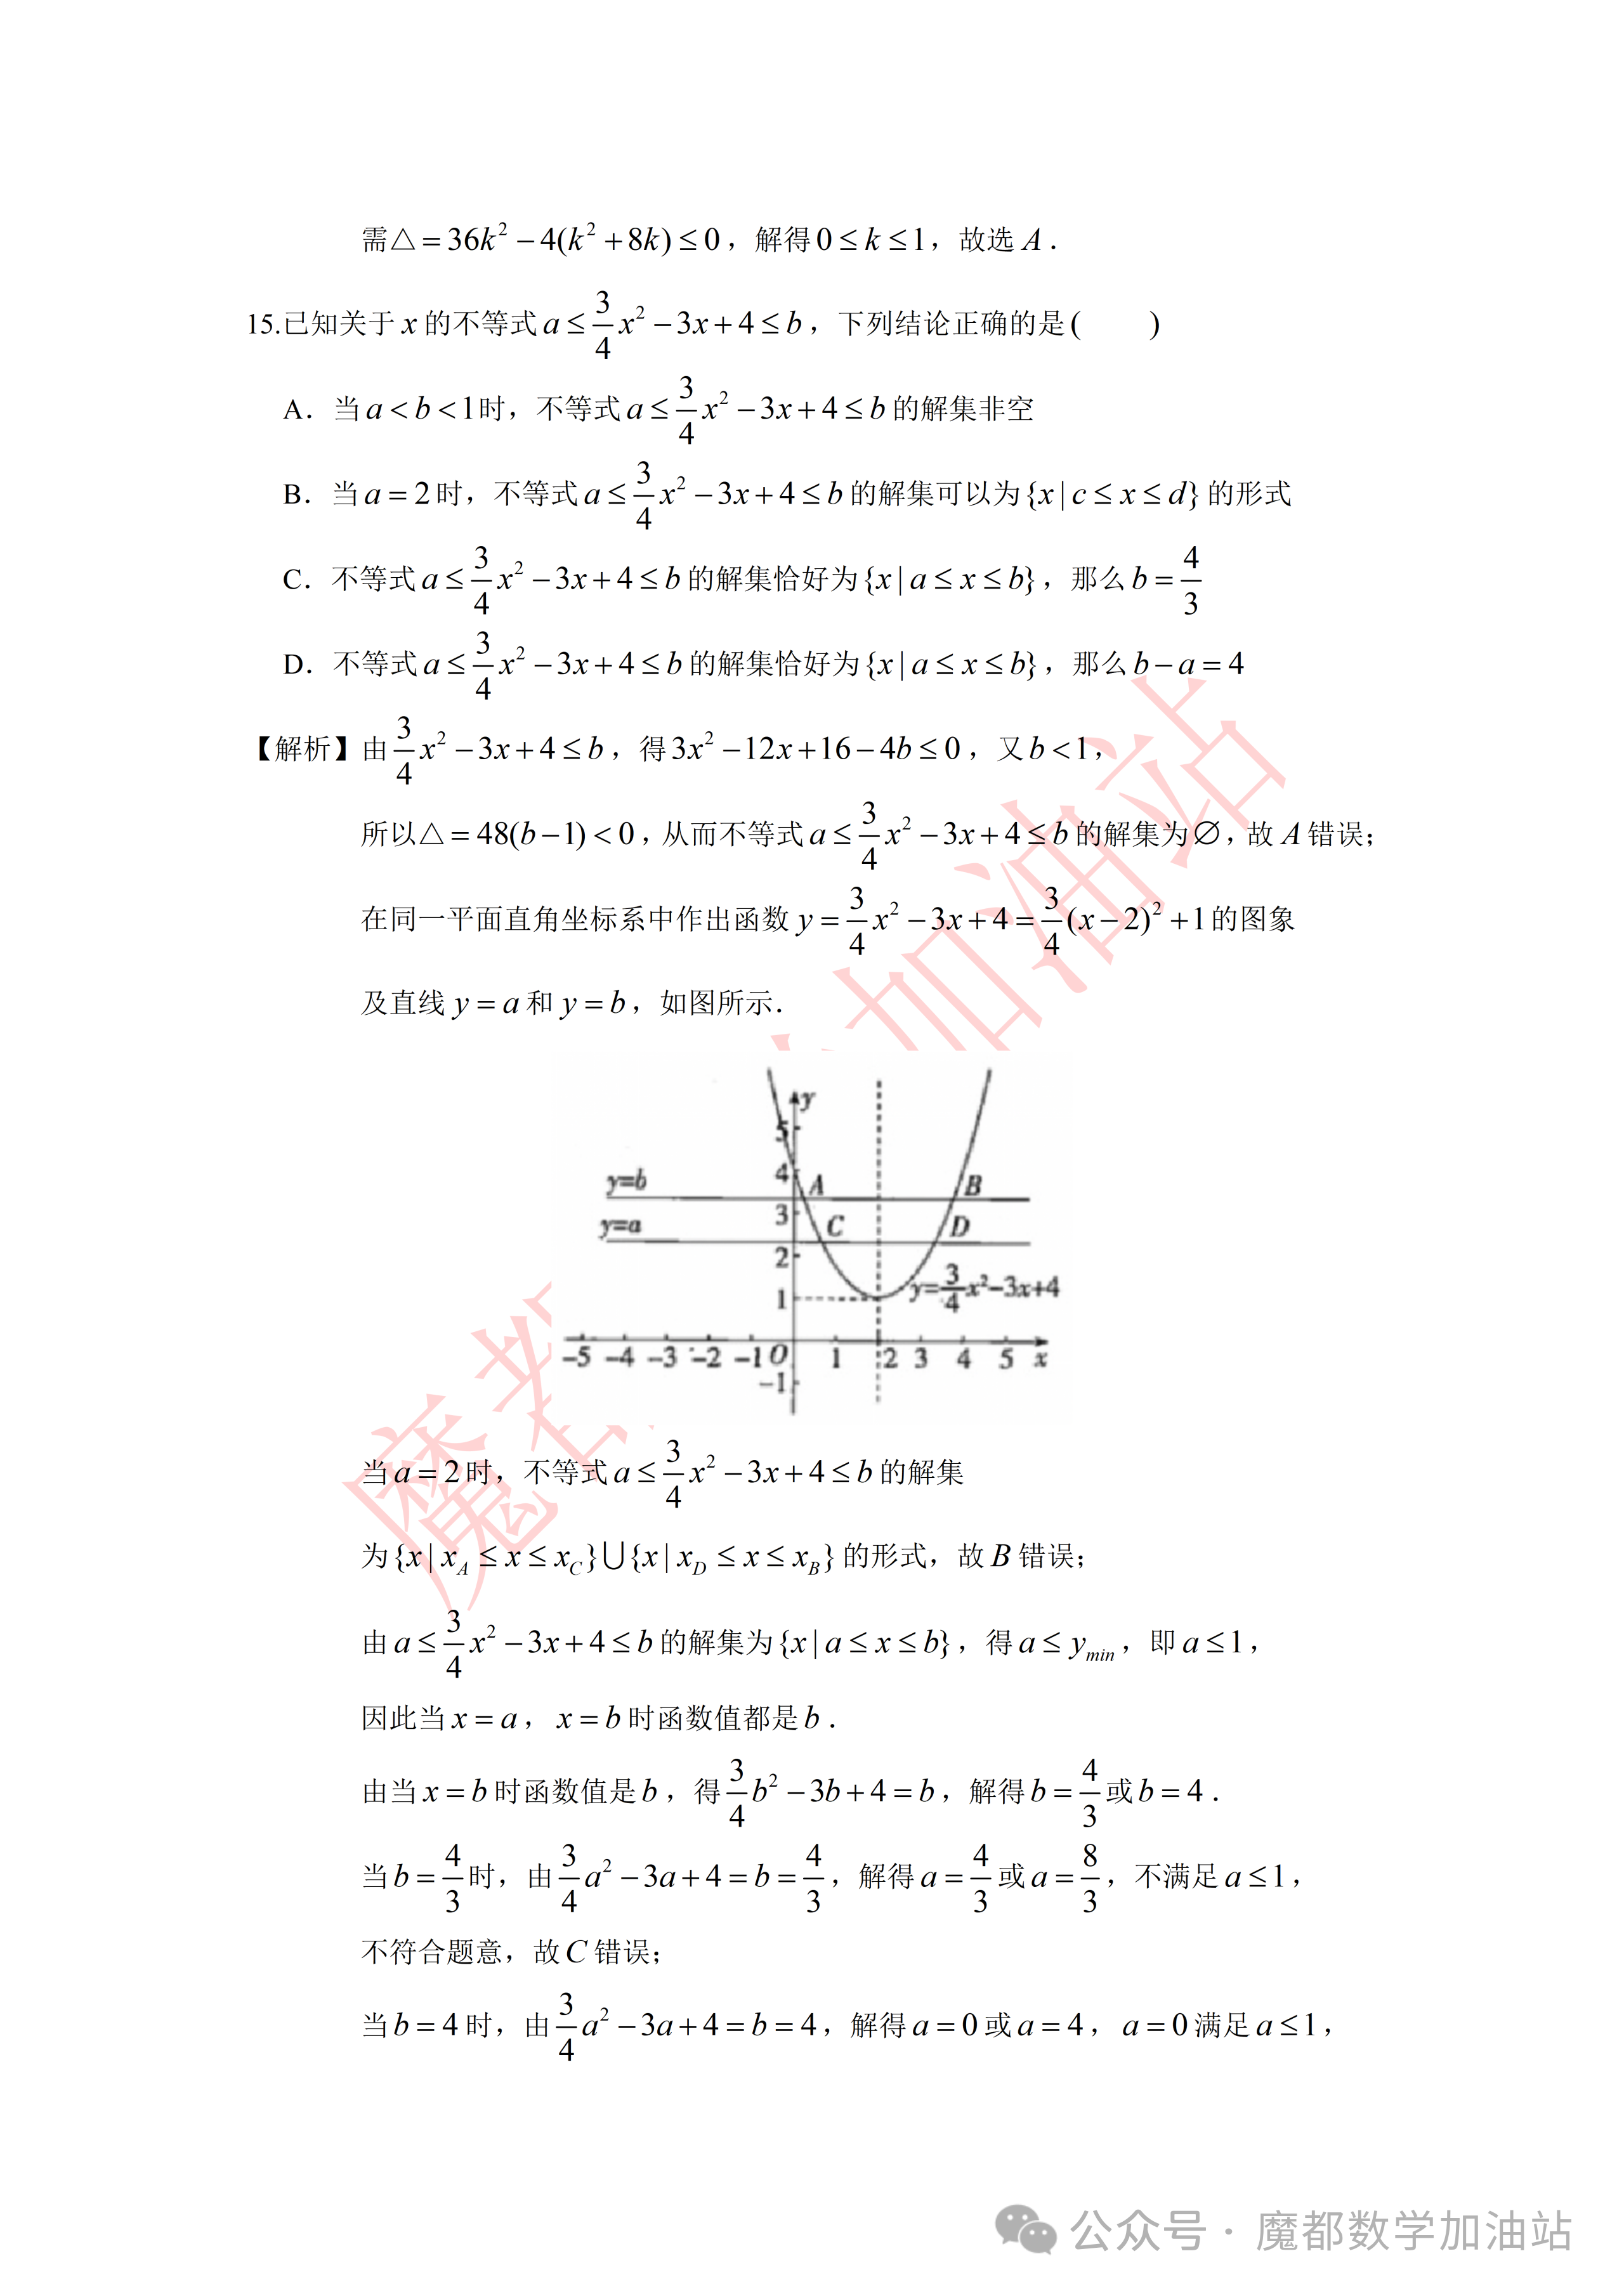
\includegraphics[width=.55\linewidth,trim=900bp 1400bp 760bp 1680bp,clip]{../原图/高一46_交附闵行_国庆作业3/05.png}
\end{center}
\step{当 $a=2$ 时，不等式 $a\leqslant\dfrac34x^2-3x+4\leqslant b$ 的解集为
$\{x\mid x_A\leqslant x\leqslant x_C\}\cup\{x\mid x_D\leqslant x\leqslant x_B\}$ 的形式，故 $B$ 错误；}
\step{由 $a\leqslant\dfrac34x^2-3x+4\leqslant b$ 的解集恰好为 $\{x\mid a\leqslant x\leqslant b\}$ 的形式，得 $a\leqslant y_{\min}$，即 $a\leqslant1$，}
\step{因为当 $x=a$、$x=b$ 时函数值都是 $b$，当 $x=a$ 时，$\dfrac34a^2-3a+4=b$；当 $x=b$ 时，$\dfrac34b^2-3b+4=b$，}
\step{解得 $b=\dfrac43$ 或 $b=4$，}
\step{当 $b=\dfrac43$ 时，由 $\dfrac34a^2-3a+4=b$，解得 $a=\dfrac43$ 或 $a=\dfrac83$，不符合题意，故 $C$ 错误；}
\step{当 $b=4$ 时，由 $\dfrac34a^2-3a+4=b$，解得 $a=0$ 或 $a=4$，$a=0$ 满足 $a\leqslant1$，故 $D$ 正确；}
\step{故选 $D$.}
\solend
\fi

\item 已知 $x$、$y\in(0,+\infty)$，则 $(x-y)^2+2y+1-x+\dfrac4x$ 的最小值为\mbox{（\quad）}

\keepwithprev
A. $1$\qquad B. $2$\qquad C. $3$\qquad D. $4$

\ans{$D$}

\ifanswer
\solbegin
\step{因为 $(x-y)^2+2y+1-x+\dfrac4x=(x-y-1)^2+x+\dfrac4x$，}
\step{当且仅当 $x-y-1=0$，且 $x=\dfrac4x$ 时取等号，}
\step{又因为 $x+\dfrac4x\geqslant2\sqrt{x\cdot\dfrac4x}=4$，当且仅当 $x=2$ 时取等号，}
\step{故选 $D$.}
\solend
\fi

\end{enumerate}

\bigsec{三、解答题}

\begin{enumerate}
\setcounter{enumi}{16}

\item 设集合 $A=\left\{x\middle|\dfrac{x-3}{x-1}<0\right\}$，$B=\{x\mid x^2-2ax+a^2-1>0\}$.
\begin{enumerate}[label=(\arabic*)]
\item 若 $a=3$，求 $A\cup B$；
\item 若“$x\in A$”是“$x\in B$”的充分条件，求实数 $a$ 的取值范围.
\end{enumerate}

\ifanswer
\solbegin
% 注：原卷题干为 a^2-1，故 a=3 时常数项为 8；题干与本步一致。
\stepm{(1)}{当 $a=3$ 时，$B=\{x\mid x^2-6x+8>0\}=\{x\mid x<2\text{ 或 }x>4\}$；}
\step{因为 $A=\left\{x\middle|\dfrac{x-3}{x-1}<0\right\}=\{x\mid(x-1)(x-3)<0\}=\{x\mid1<x<3\}$，}
\step{所以 $A\cup B=\{x\mid x<2\text{ 或 }x>4\}\cup\{x\mid1<x<3\}
=\{x\mid x<3\text{ 或 }x>4\}$.}
\stepm{(2)}{因为“$x\in A$”是“$x\in B$”的充分条件，所以 $A\subseteq B$，}
\step{因 $A=\left\{x\middle|\dfrac{x-3}{x-1}<0\right\}
=\{x\mid(x-1)(x-3)<0\}=\{x\mid1<x<3\}$，}
\step{所以 $A\subseteq B=\{x\mid x<a-1\text{ 或 }x>a+1\}$，}
\step{要使 $A\subseteq B$，需有 $a-1\geqslant3$ 或 $a+1\leqslant1$，}
\step{所以 $a\geqslant4$ 或 $a\leqslant0$，故 $a$ 的取值范围为 $\{a\mid a\geqslant4\text{ 或 }a\leqslant0\}$.}
\solend
\fi

\ansspace[6]

\item 某学校引入种植类劳动教育课程，打算围成如图所示的四块全等的长方形田地种植不同种类的蔬菜，其中一面可以利用原有的墙（足够长），其他各面需要用篱笆围成，设其中一块田地为矩形 $ABCD$.

\begin{center}
% 原图第 6 页配图直接裁取。
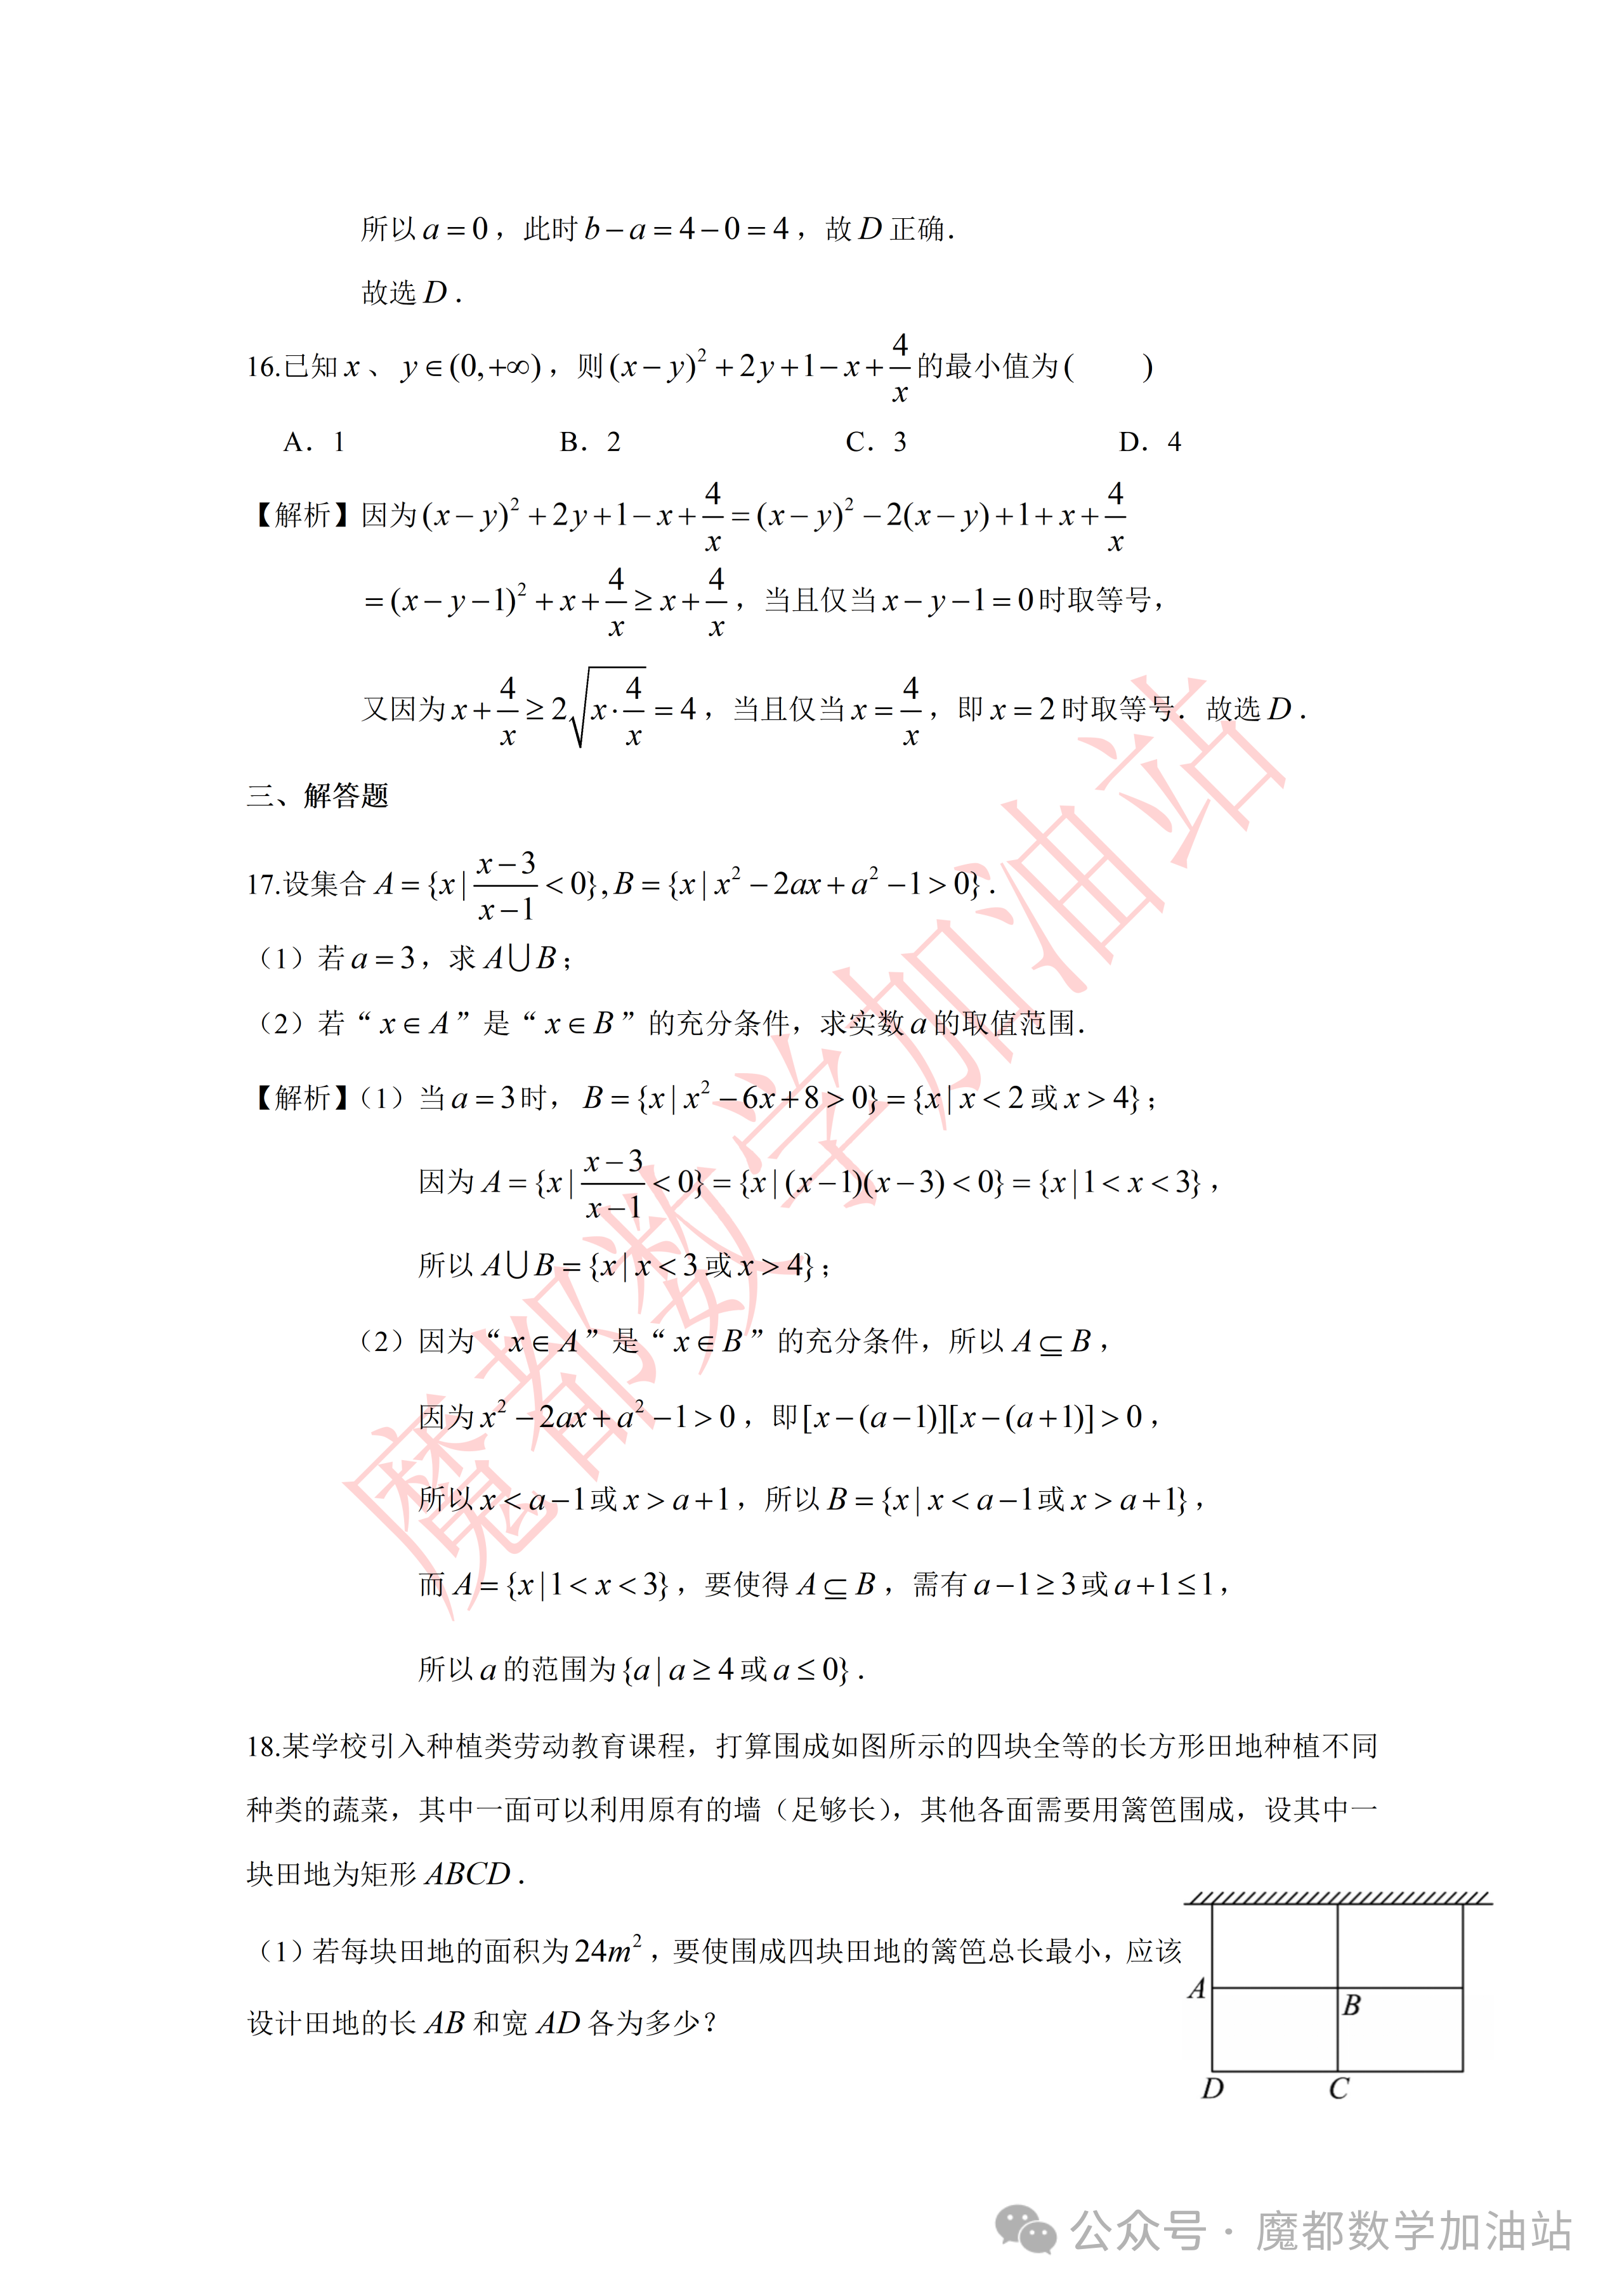
\includegraphics[width=.33\linewidth,trim=1866bp 220bp 210bp 2960bp,clip]{../原图/高一46_交附闵行_国庆作业3/06.png}
\end{center}

\begin{enumerate}[label=(\arabic*)]
\item 若每块田地的面积为 $24\,\text{m}^2$，要使围成四块田地的篱笆总长最小，应该设计田地的长 $AB$ 和宽 $AD$ 各为多少？
\item 现有 $40\,\text{m}$ 长的篱笆，要使每块田地的面积最大，应该设计田地的长 $AB$ 和宽 $AD$ 各为多少？
\end{enumerate}

\ifanswer
\solbegin
\stepm{(1)}{设 $AB$ 长为 $x\,\text{m}$，$AD$ 宽为 $y\,\text{m}$，由题意得 $xy=24$，篱笆总长为 $4x+6y$，}
\step{$4x+6y\geqslant2\sqrt{4x\cdot6y}=2\sqrt{24xy}=48$，}
\step{当且仅当 $4x=6y$ 时取等号，解得 $x=6$，$y=4$，}
\step{所以田地的长 $AB$ 为 $6\,\text{m}$，宽 $AD$ 为 $4\,\text{m}$.}
\stepm{(2)}{设 $AB$ 长为 $a\,\text{m}$，$AD$ 宽为 $b\,\text{m}$，由篱笆总长 $4a+6b=40$，即 $2a+3b=20$，}
\step{将 $a=\dfrac{20-3b}{2}$ 代入每块田地面积 $ab$，得 $ab=\dfrac12b(20-3b)=-\dfrac32b^2+10b$，}
\step{当 $b=\dfrac{10}{3}$ 时，$ab$ 最大，此时 $a=5$，}
\step{所以田地的长 $AB$ 为 $5\,\text{m}$，宽 $AD$ 为 $\dfrac{10}{3}\,\text{m}$.}
\solend
\fi

\ansspace[8]

\item 已知 $x_1$、$x_2$ 是一元二次方程 $4kx^2-4kx+k+1=0$ 的两个不等实数根.
\begin{enumerate}[label=(\arabic*)]
\item 若 $x_1$、$x_2$ 均为正根，求实数 $k$ 的取值范围；
\item 求使 $\dfrac{x_1}{x_2}+\dfrac{x_2}{x_1}-2$ 的值为整数 $k$ 的整数值.
\end{enumerate}

\ifanswer
\solbegin
\stepm{(1)}{由题意，$x_1$、$x_2$ 是方程 $4kx^2-4kx+k+1=0$ 的两个不等实数根，}
\step{故 $k\neq0$，$\Delta=(-4k)^2-16k(k+1)>0$，得 $-16k>0$，所以 $k<0$，}
\step{又 $x_1+x_2=1$，$x_1x_2=\dfrac{k+1}{4k}>0$，得 $k+1<0$，}
\step{所以 $k$ 的取值范围为 $(-\infty,-1)$.}
\stepm{(2)}{由题意，}
\step{$\dfrac{x_1}{x_2}+\dfrac{x_2}{x_1}-2
=\dfrac{x_1^2+x_2^2-2x_1x_2}{x_1x_2}
=\dfrac{(x_1+x_2)^2-4x_1x_2}{x_1x_2}$，}
\step{又 $x_1+x_2=1$，$x_1x_2=\dfrac{k+1}{4k}$，}
\step{则 $\dfrac{x_1}{x_2}+\dfrac{x_2}{x_1}-2=-\dfrac4{k+1}$，}
\step{由于 $-\dfrac4{k+1}$ 为整数，故 $k+1$ 只能取 $\pm1$、$\pm2$、$\pm4$，又 $k<-1$，}
\step{所以整数 $k$ 的值为 $-2$、$-3$、$-5$.}
\solend
\fi

\ansspace[8]

\item 已知 $a>0$，$b>0$，且 $2a+3b=3$.
\begin{enumerate}[label=(\arabic*)]
\item 求 $ab$ 的最大值；
\item 求 $a-\dfrac1{6b}$ 的最大值；
\item 求 $\dfrac2a+\dfrac3{b+1}$ 的最小值.
\end{enumerate}

\ifanswer
\solbegin
\stepm{(1)}{由 $2a+3b=3$，得 $3=2a+3b\geqslant2\sqrt{6ab}$，}
\step{所以 $ab\leqslant\dfrac38$，当且仅当 $2a=3b=\dfrac32$ 时取等号，}
\step{故 $ab$ 的最大值为 $\dfrac38$.}
\stepm{(2)}{由 $2a+3b=3$，得 $a=\dfrac32-\dfrac32b$，}
\step{则 $a-\dfrac1{6b}=\dfrac32-\dfrac32b-\dfrac1{6b}$，}
\step{由基本不等式，$\dfrac32b+\dfrac1{6b}\geqslant2\sqrt{\dfrac32b\cdot\dfrac1{6b}}=1$，}
\step{当且仅当 $\dfrac32b=\dfrac1{6b}$，即 $b=\dfrac13$、$a=1$ 时取等号，}
\step{所以 $a-\dfrac1{6b}$ 的最大值为 $\dfrac12$.}
\stepm{(3)}{由 $2a+3b=3$，得 $2a+3(b+1)=6$，}
\step{$\dfrac2a+\dfrac3{b+1}
=\dfrac16\left(2a+3(b+1)\right)\left(\dfrac2a+\dfrac3{b+1}\right)$}
\step{$=\dfrac16\left(13+\dfrac{6(b+1)}a+\dfrac{6a}{b+1}\right)
\geqslant\dfrac16\left(13+2\sqrt{\dfrac{6(b+1)}a\cdot\dfrac{6a}{b+1}}\right)=\dfrac{25}{6}$，}
\step{当且仅当 $a=b+1$，即 $a=\dfrac65$、$b=\dfrac15$ 时取等号，}
\step{所以 $\dfrac2a+\dfrac3{b+1}$ 的最小值为 $\dfrac{25}{6}$.}
\solend
\fi

\ansspace[8]

\item 已知 $U=\R$ 为全集，集合 $A=\{s^2+3t^2\mid s,t\in U\}$.
\begin{enumerate}[label=(\arabic*)]
\item 设 $U=\{1,3,5\}$，求集合 $A$ 的元素个数；
\item 设 $U=\Z$，证明：若 $x\in A$，则 $7x\in A$；
\item 设 $U=\R$，$x$、$y\in A$，且 $x=m^2+3n^2$，$y=p^2+3q^2$，若 $mp-3nq=\sqrt3$，求 $x+y+mq+np$ 的最小值.
\end{enumerate}

\ifanswer
\solbegin
\stepm{(1)}{当 $s=1$，$t=1$ 时，$s^2+3t^2=1+3=4$；}
\step{当 $s=1$，$t=3$ 时，$s^2+3t^2=1+27=28$；}
\step{当 $s=1$，$t=5$ 时，$s^2+3t^2=1+75=76$；}
\step{当 $s=3$，$t=1$ 时，$s^2+3t^2=9+3=12$；}
\step{当 $s=3$，$t=3$ 时，$s^2+3t^2=9+27=36$；}
\step{当 $s=3$，$t=5$ 时，$s^2+3t^2=9+75=84$；}
\step{当 $s=5$，$t=1$ 时，$s^2+3t^2=25+3=28$；}
\step{当 $s=5$，$t=3$ 时，$s^2+3t^2=25+27=52$；}
\step{当 $s=5$，$t=5$ 时，$s^2+3t^2=25+75=100$，}
\step{所以 $A=\{4,12,28,36,52,76,84,100\}$，有 $8$ 个元素.}
\stepm{(2)}{因为 $U=\Z$，$x\in A$，设 $x=s^2+3t^2$，}
\step{则 $7x=7(s^2+3t^2)=(2s+3t)^2+3(s-2t)^2\in A$，}
\step{所以 $7x\in A$.}
\stepm{(3)}{因为 $x=m^2+3n^2$，$y=p^2+3q^2$，}
\step{$xy=(m^2+3n^2)(p^2+3q^2)=3(mq+np)^2+(mp-3nq)^2$，}
\step{设 $mq+np=b$，则 $xy=3b^2+3$，所以 $y=\dfrac{3b^2+3}{x}$，}
\step{于是 $x+y+mq+np=x+\dfrac{3b^2+3}{x}+b\geqslant2\sqrt{3b^2+3}+b$，}
\step{设 $2\sqrt{3b^2+3}+b=t$，整理得 $11b^2+2bt+12-t^2=0$，}
\step{判别式法，$\Delta=4t^2-44(12-t^2)\geqslant0$，得 $t\geqslant\sqrt{11}$，}
\step{即 $(x+y+mq+np)_{\min}=\sqrt{11}$，所以 $x+y+mq+np$ 的最小值为 $\sqrt{11}$.}
\solend
\fi

\ansspace*[10]

\end{enumerate}

\end{document}
"
%
% 原始材料：微信公众号“魔都数学加油站”，作者破晓，2026-10-02 17:56 发布。
% 原文标题：“27学年高一46——2026-2027你那上海市交附闵行高一上国庆作业3”
% （公众号标题中的“你那”照录，系原文标题字样）；原文链接：
% http://mp.weixin.qq.com/s?__biz=Mzg4ODU1ODMxOQ==&mid=2247591657&idx=3&sn=a894d1a16611283a61b3eaba32a3f24c&chksm=cee83366c6a55381b370069f84ef63d20251f94608bb37cc4ec2d66227401bd147f4f6bd8256&scene=126&sessionid=1790935402&subscene=7&clicktime=1790937618&enterid=1790937618#rd
% 正文为 9 张 PNG 页，按页序读取原图；第 01、02、07 页 4762×6735，
% 第 03—06、08、09 页 2560×3620。卷面标题照原卷印作“2026-2027 年交附闵行高一上国庆作业 3”。
% 原文从第 3 题起，题号照原卷保留；正文为讲评版，答案、解析依原卷顺序录入。
% 水印及页脚公众号标识不录入。卷面插图直接裁取对应原图页，不另制图片文件。
%
% 与原卷的排版差异：
%   ① 原卷按“一、填空题”“二、选择题”“三、解答题”分节，本稿沿用原节与原题号，
%      只改排为全稿统一的大节样式；
%   ② 原卷答案与解析依页面位置分布，本稿按 common.sty 统一置于答案版；
%   ③ 原卷副标题未印，本稿按“知识模块”口径标作“集合与常用逻辑用语、不等式”。
%
% 原卷存疑一处（照抄未改，见第 12 题题干及解析处注释）：
%   第 12 题题干同时给出 x∈Z，却称不等式组有“50 个不等的实数解”；解析按整数根计数。
%   此处题干与解析的原文不一致，本稿均照录。
% 第 17 题曾疑似有常数项不一致：复核原图题干为 a^2-1，a=3 时常数项确为 8，
% 与解析相符；不将其记作原卷错误。
%
\documentclass[a4paper,11pt]{article}
\usepackage{common}

\begin{document}

\examtitlest[3]{2026--2027 年交附闵行高一上国庆作业 3}{集合与常用逻辑用语、不等式}

\bigsec{一、填空题}

\begin{enumerate}
\setcounter{enumi}{2}

\item 不等式 $\dfrac{x^2-10}{x+2}\geqslant1$ 的解集为\blankline[4.4em].

\ifanswer
\ans{$\{x\mid-3\leqslant x<-2\text{ 或 }x\geqslant4\}$}
\solbegin
\step{不等式 $\dfrac{x^2-10}{x+2}\geqslant1$，移项得 $\dfrac{x^2-10}{x+2}-1\geqslant0$，}
\step{通分得 $\dfrac{x^2-x-12}{x+2}\geqslant0$，即 $\dfrac{(x-4)(x+3)}{x+2}\geqslant0$，}
\step{解得 $-3\leqslant x<-2$ 或 $x\geqslant4$，}
\step{故不等式的解集为 $\{x\mid-3\leqslant x<-2\text{ 或 }x\geqslant4\}$.}
\solend
\fi

\item $|x-3|+|x-5|\geqslant2$，当等号成立时，$x$ 的范围是\blankline[4.4em].

\ifanswer
\ans{$[3,5]$}
\fi

\item 若直角三角形斜边长等于 $4\sqrt2\,\text{cm}$，则直角三角形面积的最大值为\blankline[4.4em].

\ifanswer
\solbegin
\step{设 $Rt\triangle ABC$ 中，$C=90^\circ$，则 $c=\sqrt{a^2+b^2}=4\sqrt2$，所以 $a^2+b^2=32$，}
\step{由基本不等式得 $a^2+b^2\geqslant2ab$，当且仅当 $a=b=4$ 时取等号，}
\step{所以 $\triangle ABC$ 的面积 $S=\dfrac12ab\leqslant8$，}
\step{当且仅当 $a=b=4$ 时，$\triangle ABC$ 的面积最大值为 $8$.}
\solend
\fi

\item 不等式 $(x-1)(2-x)>0$ 的解集为\blankline[4.4em].

\ifanswer
\solbegin
\step{$(x-1)(2-x)>0\Rightarrow(x-1)(x-2)<0$，}
\step{故不等式的解集为 $\{x\mid1<x<2\}$.}
\solend
\fi

\item 已知集合 $A=\{1,2\}$，$B=\{x\mid x^2-2mx+m=0\}$，$A\cup B=A$，则实数 $m$ 的取值范围为\blankline[4.4em].

\ifanswer
\solbegin
\step{因为 $A\cup B=A$，所以 $B\subseteq A$，}
\step{当 $B=\varnothing$ 时，$\Delta=(-2m)^2-4m<0$，解得 $0<m<1$，}
\step{当 $B$ 为单元素集时，$\Delta=0$，解得 $m=0$ 或 $m=1$，}
\step{当 $m=0$ 时，方程 $x^2=0$，解得 $x=0$，此时 $B=\{0\}$，不满足 $B\subseteq A$；}
\step{当 $m=1$ 时，方程 $x^2-2x+1=0$，解得 $x=1$，此时 $B=\{1\}$，满足 $B\subseteq A$；}
\step{当 $B=\{1,2\}$ 时，由韦达定理得 $1+2=2m$，$1\times2=m$，无解，}
\step{综上所述，实数 $m$ 的取值范围为 $\{m\mid0<m\leqslant1\}$.}
\solend
\fi

\item 设 $a$、$b$、$c\in\R^+$，若 $a+b+c=1$，则 $\dfrac1a+\dfrac1b+\dfrac1c\geqslant$\blankline[4.4em].

\ifanswer
\solbegin
\step{因为 $a$、$b$、$c\in\R^+$，且 $a+b+c=1$，}
\step{所以 $\dfrac1a+\dfrac1b+\dfrac1c=(a+b+c)\left(\dfrac1a+\dfrac1b+\dfrac1c\right)$}
\step{$=3+\dfrac ab+\dfrac ba+\dfrac ac+\dfrac ca+\dfrac bc+\dfrac cb$，}
\step{由基本不等式得 $\dfrac ab+\dfrac ba\geqslant2$，$\dfrac ac+\dfrac ca\geqslant2$，$\dfrac bc+\dfrac cb\geqslant2$，}
\step{所以 $\dfrac1a+\dfrac1b+\dfrac1c\geqslant9$，当且仅当 $a=b=c=\dfrac13$ 时取等号，}
\step{所以 $\dfrac1a+\dfrac1b+\dfrac1c$ 的最小值为 $9$.}
\solend
\fi

\item 已知 $-1\leqslant x+y\leqslant2$，$-2\leqslant x-y\leqslant1$，则 $x-2y$ 的范围为\blankline[4.4em].

\ifanswer
\solbegin
\step{设 $x-2y=m(x+y)+n(x-y)$，}
\step{则 $x-2y=(m+n)x+(m-n)y$，所以 $m+n=1$，$m-n=-2$，}
\step{解得 $m=-\dfrac12$，$n=\dfrac32$，}
\step{所以 $x-2y=-\dfrac12(x+y)+\dfrac32(x-y)$，}
\step{因为 $-1\leqslant x+y\leqslant2$，$-2\leqslant x-y\leqslant1$，}
\step{所以 $-4\leqslant x-2y\leqslant2$，即 $x-2y$ 的范围为 $[-4,2]$.}
\solend
\fi

\item 设集合 $A=\{1,2,m\}$，其中 $m$ 为实数，令 $B=\{a^2\mid a\in A\}$，$C=A\cup B$. 若 $C$ 中所有元素之和为 $6$，则 $C$ 中的所有元素之积为\blankline[4.4em].

\ifanswer
\solbegin
\step{因为 $A=\{1,2,m\}$，所以 $B=\{a^2\mid a\in A\}=\{1,4,m^2\}$，$m\neq1$，$m\neq2$，}
\step{又 $C=A\cup B$，所以 $1\in C$，$4\in C$，$m^2\in C$，}
\step{若 $m^2=1$，则 $m=-1$ 或 $m=1$（舍），当 $m=-1$ 时，$C=\{1,2,4,-1\}$，$C$ 中所有元素之和为 $6$，}
\step{此时 $C$ 中所有元素之积为 $-8$；}
\step{若 $m^2=2$，则 $m=-\sqrt2$ 或 $m=\sqrt2$，$C$ 中所有元素之和不符合题意；}
\step{若 $m^2=4$，则 $m=-2$ 或 $m=2$，此时 $C=\{1,2,4,-2\}$ 或 $C=\{1,2,4\}$，所有元素之和不符合题意；}
\step{若 $m^2\neq1$，$m^2\neq2$，$m^2\neq4$，则 $C=\{1,2,4,m,m^2\}$，}
\step{所以 $1+2+4+m+m^2=6$，即 $m^2+m+1=0$，无解，}
\step{综上所述，$C$ 中所有元素之积为 $-8$.}
\solend
\fi

\item 若对任意实数 $x>0$，$y>0$，不等式 $x+\sqrt{xy}\leqslant a(x+y)$ 恒成立，则实数 $a$ 的最小值为\blankline[4.4em].

\ifanswer
\solbegin
\step{由不等式 $x+\sqrt{xy}\leqslant a(x+y)$ 对任意实数 $x>0$，$y>0$ 恒成立，}
\step{得 $a\geqslant\dfrac{x+\sqrt{xy}}{x+y}$，}
\step{设 $\sqrt{\dfrac yx}=t>0$，则 $a\geqslant\dfrac{1+t}{1+t^2}$，}
\step{$\dfrac{1+t}{1+t^2}\leqslant\dfrac{\sqrt2+1}{2}$，当且仅当 $t=\sqrt2-1$ 时取等号，}
\step{所以实数 $a$ 的最小值为 $\dfrac{\sqrt2+1}{2}$.}
\solend
\fi

% 注：原卷题干给出 x∈Z，却写“实数解”；解析按整数解计数，题干与解析不一致，照录未改。
\item 若关于 $x$ 的不等式组
$\begin{cases}x^2-3mx\geqslant4m^2\\-20<x<120\end{cases}$（$x\in\Z,m>0$）恰有 $50$ 个不等的实数解，则 $m$ 的取值范围为\blankline[4.4em]（结果用区间表示）.

\ifanswer
\solbegin
\step{由 $x^2-3mx\geqslant4m^2$ 以及 $m>0$，解得 $x\leqslant-m$ 或 $x\geqslant4m$，}
\step{由原不等式组恰有 $50$ 个不等的实数解，可画出如下解集区间：}
\begin{center}
% 原图第 4 页数轴图直接裁取。
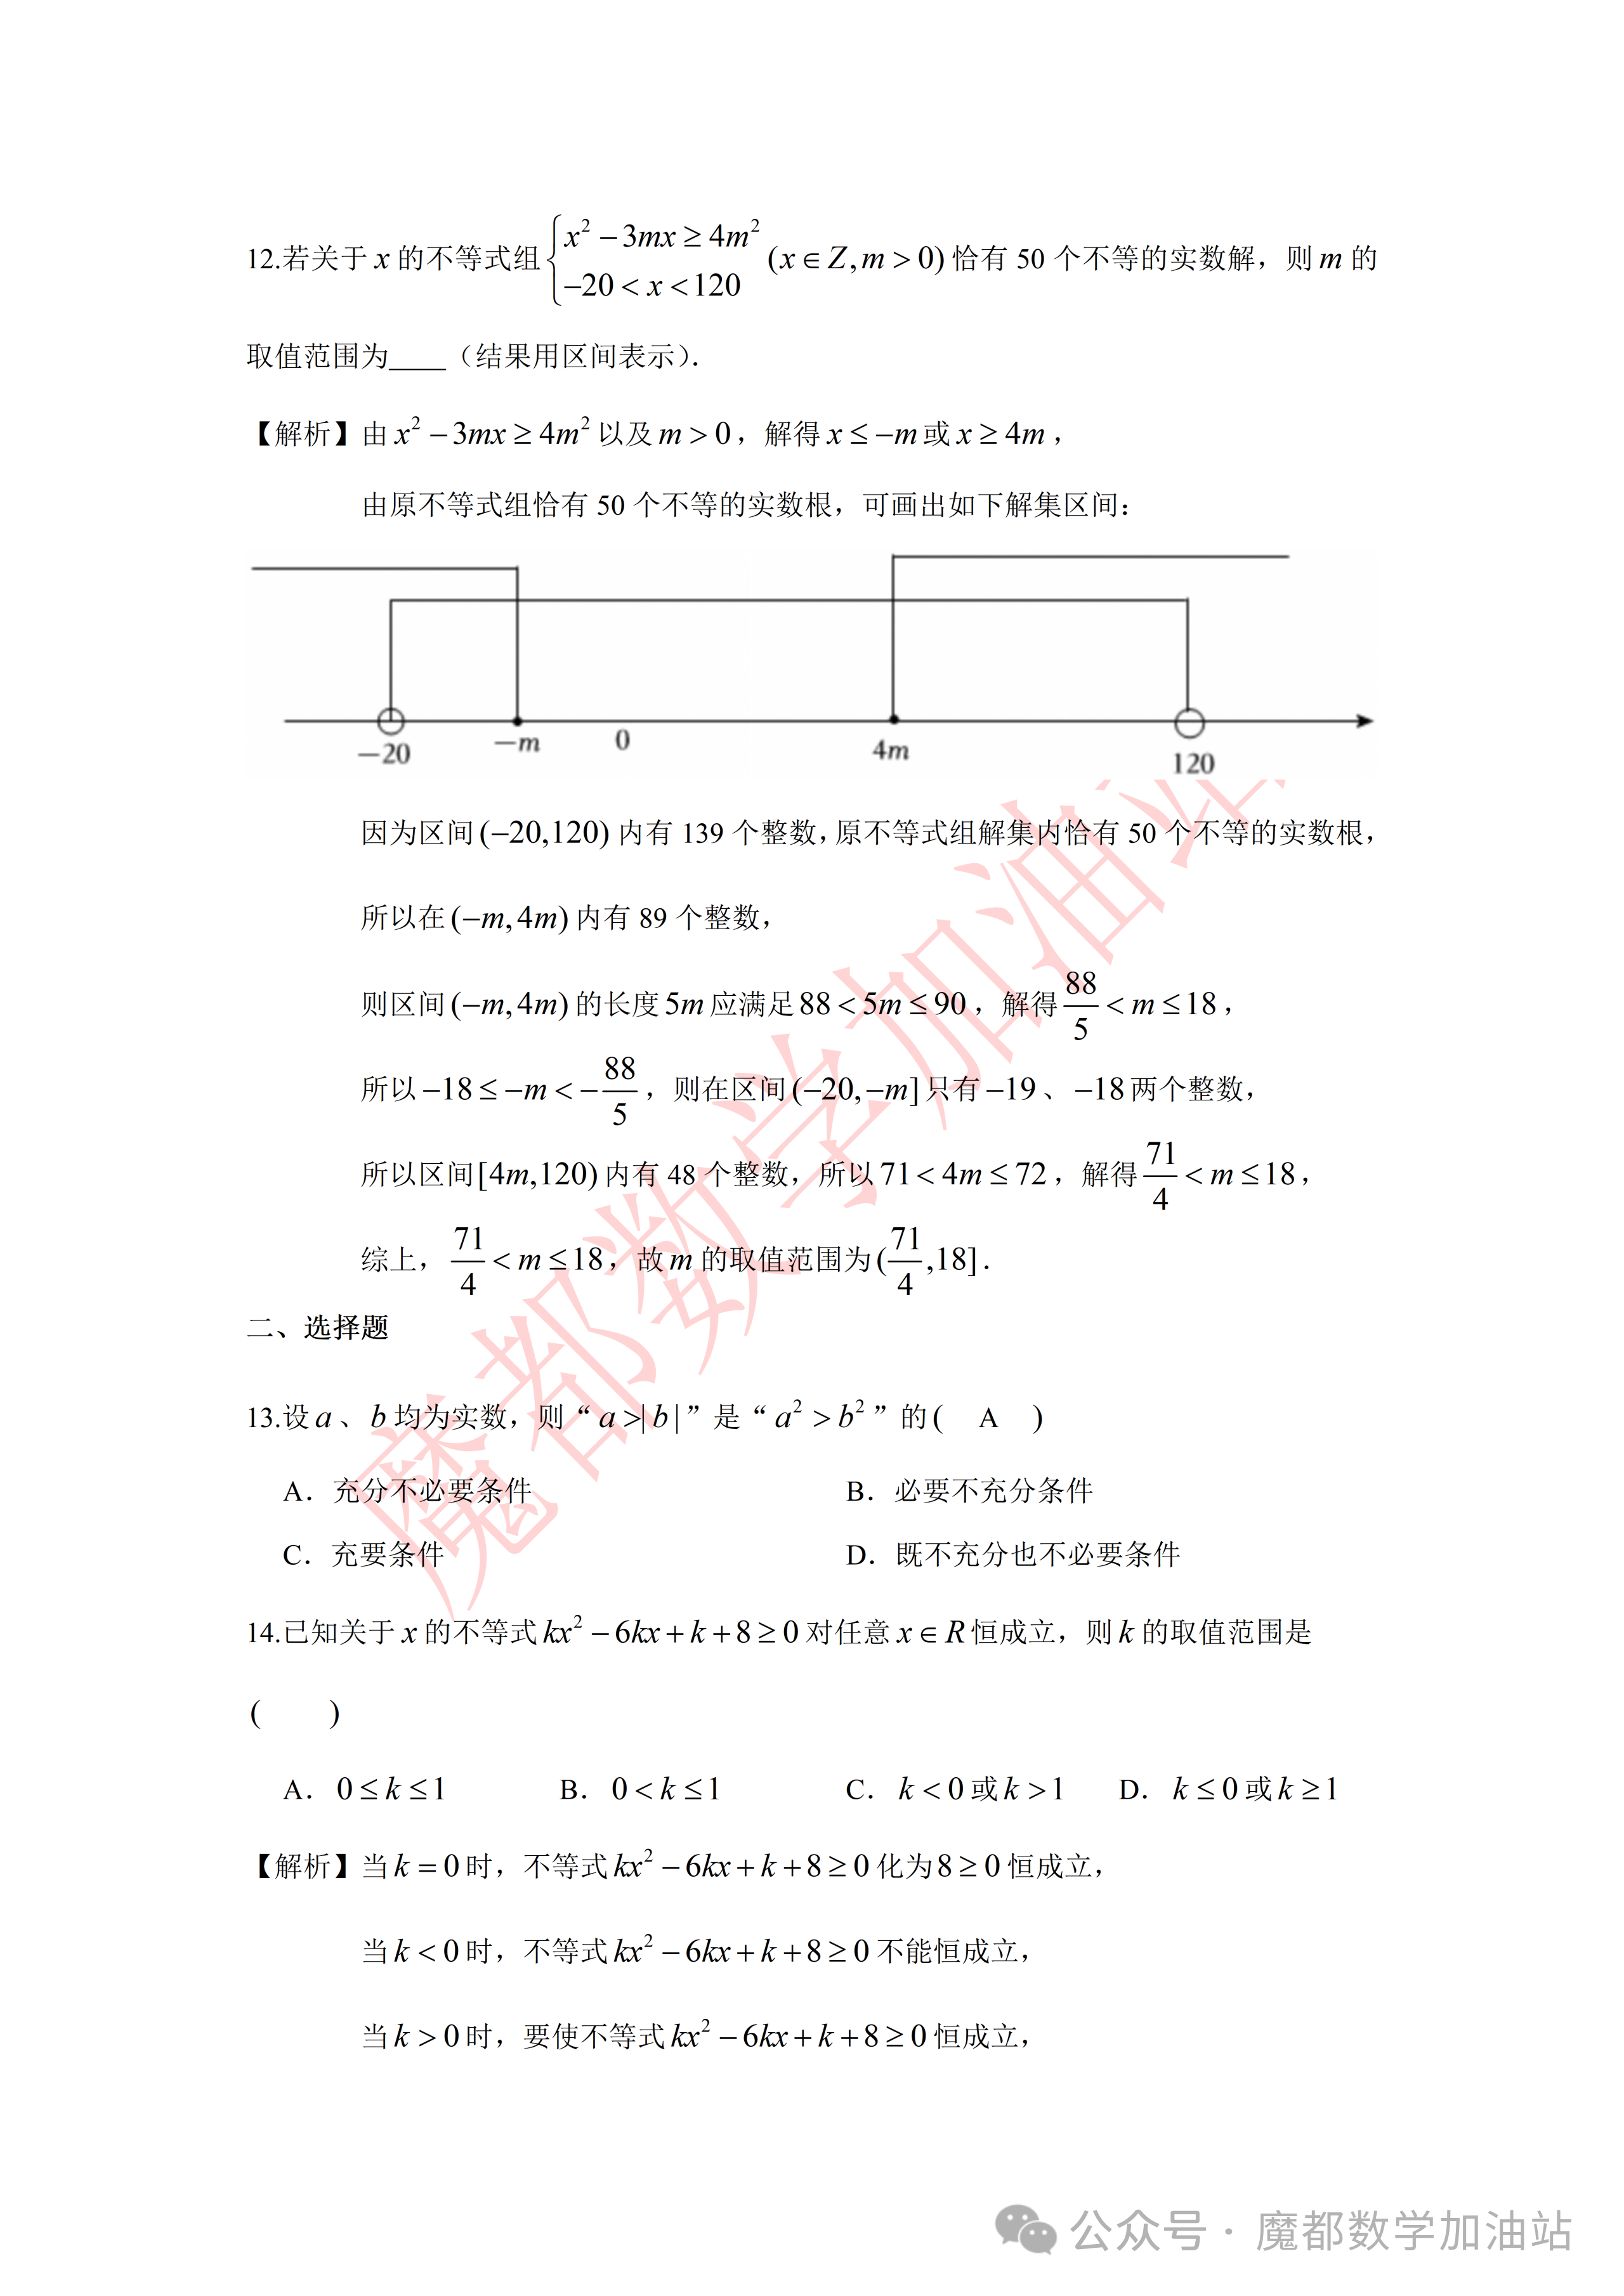
\includegraphics[width=.88\linewidth,trim=400bp 2410bp 320bp 860bp,clip]{../原图/高一46_交附闵行_国庆作业3/04.png}
\end{center}
\step{因为区间 $(-20,120)$ 内有 $139$ 个整数，原不等式组解集内有 $50$ 个不等的整数根，}
\step{所以在区间 $(-m,4m)$ 内有 $89$ 个整数，}
\step{则区间 $(-m,4m)$ 的长度 $5m$ 应满足 $88<5m\leqslant90$，解得 $\dfrac{88}{5}<m\leqslant18$，}
% 注：原卷题干称“实数解”，本行及后文按原卷解析照录为整数根计数。
\step{所以 $-18\leqslant-m<-\dfrac{88}{5}$，则在区间 $(-20,-m]$ 内有 $-19$、$-18$ 两个整数，}
\step{所以区间 $[4m,120)$ 内有 $48$ 个整数，}
\step{则 $71<4m\leqslant72$，解得 $\dfrac{71}{4}<m\leqslant18$，}
\step{综上，$\dfrac{71}{4}<m\leqslant18$，故 $m$ 的取值范围为 $\left(\dfrac{71}{4},18\right]$.}
\solend
\fi

\end{enumerate}

\bigsec{二、选择题}

\begin{enumerate}
\setcounter{enumi}{12}

\item 设 $a$、$b$ 均为实数，则“$a>|b|$”是“$a^2>b^2$”的\mbox{（\quad）}

\keepwithprev
A. 充分不必要条件\qquad B. 必要不充分条件

C. 充要条件\qquad\qquad D. 既不充分也不必要条件

\ans{$A$}

\item 已知关于 $x$ 的不等式 $kx^2-6kx+k+8\geqslant0$ 对任意 $x\in\R$ 恒成立，则 $k$ 的取值范围是\mbox{（\quad）}

\keepwithprev
A. $0\leqslant k\leqslant1$\qquad B. $0<k\leqslant1$

C. $k<0$ 或 $k>1$\qquad D. $k\leqslant0$ 或 $k\geqslant1$

\ans{$A$}

\ifanswer
\solbegin
\step{当 $k=0$ 时，不等式 $kx^2-6kx+k+8\geqslant0$ 化为 $8\geqslant0$ 恒成立，}
\step{当 $k<0$ 时，不等式 $kx^2-6kx+k+8\geqslant0$ 不能恒成立，}
\step{当 $k>0$ 时，要使不等式 $kx^2-6kx+k+8\geqslant0$ 恒成立，}
\step{需 $\Delta=36k^2-4(k^2+8k)\leqslant0$，解得 $0\leqslant k\leqslant1$，故选 $A$.}
\solend
\fi

\item 已知关于 $x$ 的不等式 $a\leqslant\dfrac34x^2-3x+4\leqslant b$，下列结论正确的是\mbox{（\quad）}

\keepwithprev
A. 当 $a<b<1$ 时，不等式 $a\leqslant\dfrac34x^2-3x+4\leqslant b$ 的解集非空

B. 当 $a=2$ 时，不等式 $a\leqslant\dfrac34x^2-3x+4\leqslant b$ 的解集可以为 $\{x\mid c\leqslant x\leqslant d\}$ 的形式

C. 不等式 $a\leqslant\dfrac34x^2-3x+4\leqslant b$ 的解集恰好为 $\{x\mid a\leqslant x\leqslant b\}$，那么 $b=\dfrac43$

D. 不等式 $a\leqslant\dfrac34x^2-3x+4\leqslant b$ 的解集恰好为 $\{x\mid a\leqslant x\leqslant b\}$，那么 $b-a=4$

\ans{$D$}

\ifanswer
\solbegin
\step{由 $\dfrac34x^2-3x+4\leqslant b$，得 $3x^2-12x+16-4b\leqslant0$，又 $b<1$，}
\step{所以 $\Delta=144-12(16-4b)=48(b-1)<0$，从而不等式无解，故 $A$ 错误；}
\step{在同一平面直角坐标系中作出函数 $y=\dfrac34x^2-3x+4=\dfrac34(x-2)^2+1$ 的图象及直线 $y=a$ 和 $y=b$，如图所示.}
\begin{center}
% 原图第 5 页解析配图直接裁取。
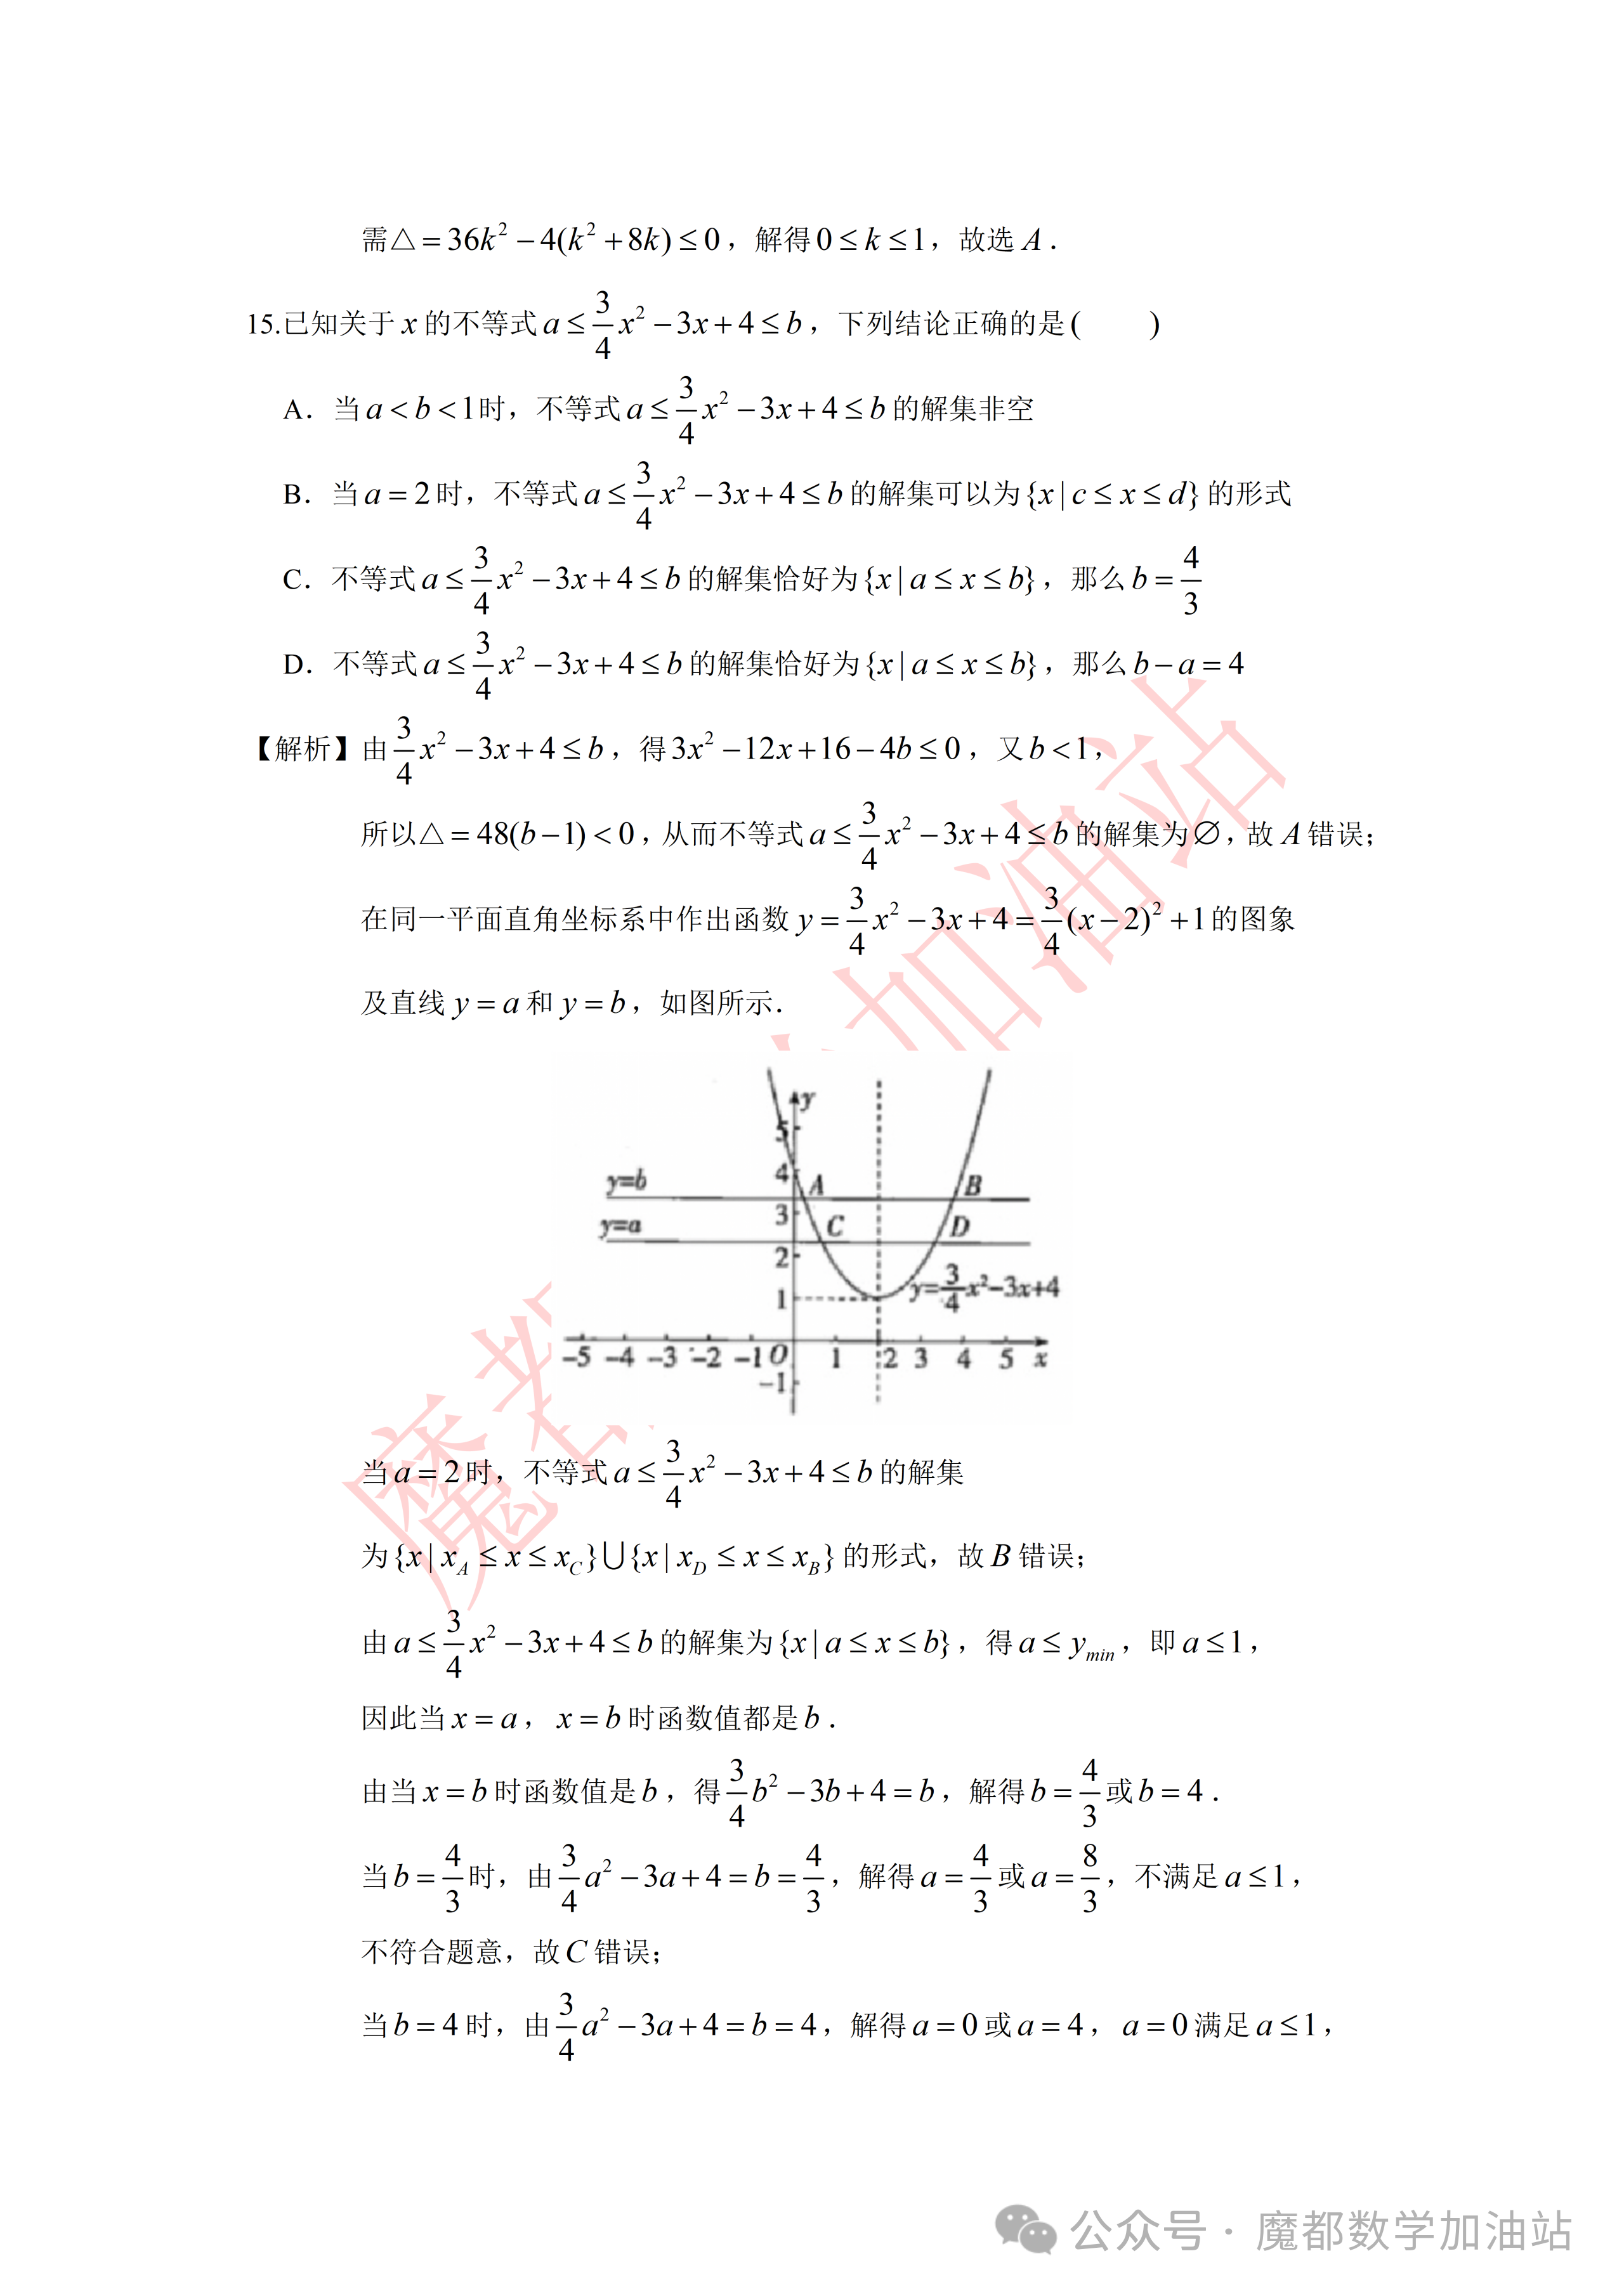
\includegraphics[width=.55\linewidth,trim=900bp 1400bp 760bp 1680bp,clip]{../原图/高一46_交附闵行_国庆作业3/05.png}
\end{center}
\step{当 $a=2$ 时，不等式 $a\leqslant\dfrac34x^2-3x+4\leqslant b$ 的解集为
$\{x\mid x_A\leqslant x\leqslant x_C\}\cup\{x\mid x_D\leqslant x\leqslant x_B\}$ 的形式，故 $B$ 错误；}
\step{由 $a\leqslant\dfrac34x^2-3x+4\leqslant b$ 的解集恰好为 $\{x\mid a\leqslant x\leqslant b\}$ 的形式，得 $a\leqslant y_{\min}$，即 $a\leqslant1$，}
\step{因为当 $x=a$、$x=b$ 时函数值都是 $b$，当 $x=a$ 时，$\dfrac34a^2-3a+4=b$；当 $x=b$ 时，$\dfrac34b^2-3b+4=b$，}
\step{解得 $b=\dfrac43$ 或 $b=4$，}
\step{当 $b=\dfrac43$ 时，由 $\dfrac34a^2-3a+4=b$，解得 $a=\dfrac43$ 或 $a=\dfrac83$，不符合题意，故 $C$ 错误；}
\step{当 $b=4$ 时，由 $\dfrac34a^2-3a+4=b$，解得 $a=0$ 或 $a=4$，$a=0$ 满足 $a\leqslant1$，故 $D$ 正确；}
\step{故选 $D$.}
\solend
\fi

\item 已知 $x$、$y\in(0,+\infty)$，则 $(x-y)^2+2y+1-x+\dfrac4x$ 的最小值为\mbox{（\quad）}

\keepwithprev
A. $1$\qquad B. $2$\qquad C. $3$\qquad D. $4$

\ans{$D$}

\ifanswer
\solbegin
\step{因为 $(x-y)^2+2y+1-x+\dfrac4x=(x-y-1)^2+x+\dfrac4x$，}
\step{当且仅当 $x-y-1=0$，且 $x=\dfrac4x$ 时取等号，}
\step{又因为 $x+\dfrac4x\geqslant2\sqrt{x\cdot\dfrac4x}=4$，当且仅当 $x=2$ 时取等号，}
\step{故选 $D$.}
\solend
\fi

\end{enumerate}

\bigsec{三、解答题}

\begin{enumerate}
\setcounter{enumi}{16}

\item 设集合 $A=\left\{x\middle|\dfrac{x-3}{x-1}<0\right\}$，$B=\{x\mid x^2-2ax+a^2-1>0\}$.
\begin{enumerate}[label=(\arabic*)]
\item 若 $a=3$，求 $A\cup B$；
\item 若“$x\in A$”是“$x\in B$”的充分条件，求实数 $a$ 的取值范围.
\end{enumerate}

\ifanswer
\solbegin
% 注：原卷题干为 a^2-1，故 a=3 时常数项为 8；题干与本步一致。
\stepm{(1)}{当 $a=3$ 时，$B=\{x\mid x^2-6x+8>0\}=\{x\mid x<2\text{ 或 }x>4\}$；}
\step{因为 $A=\left\{x\middle|\dfrac{x-3}{x-1}<0\right\}=\{x\mid(x-1)(x-3)<0\}=\{x\mid1<x<3\}$，}
\step{所以 $A\cup B=\{x\mid x<2\text{ 或 }x>4\}\cup\{x\mid1<x<3\}
=\{x\mid x<3\text{ 或 }x>4\}$.}
\stepm{(2)}{因为“$x\in A$”是“$x\in B$”的充分条件，所以 $A\subseteq B$，}
\step{因 $A=\left\{x\middle|\dfrac{x-3}{x-1}<0\right\}
=\{x\mid(x-1)(x-3)<0\}=\{x\mid1<x<3\}$，}
\step{所以 $A\subseteq B=\{x\mid x<a-1\text{ 或 }x>a+1\}$，}
\step{要使 $A\subseteq B$，需有 $a-1\geqslant3$ 或 $a+1\leqslant1$，}
\step{所以 $a\geqslant4$ 或 $a\leqslant0$，故 $a$ 的取值范围为 $\{a\mid a\geqslant4\text{ 或 }a\leqslant0\}$.}
\solend
\fi

\ansspace[6]

\item 某学校引入种植类劳动教育课程，打算围成如图所示的四块全等的长方形田地种植不同种类的蔬菜，其中一面可以利用原有的墙（足够长），其他各面需要用篱笆围成，设其中一块田地为矩形 $ABCD$.

\begin{center}
% 原图第 6 页配图直接裁取。
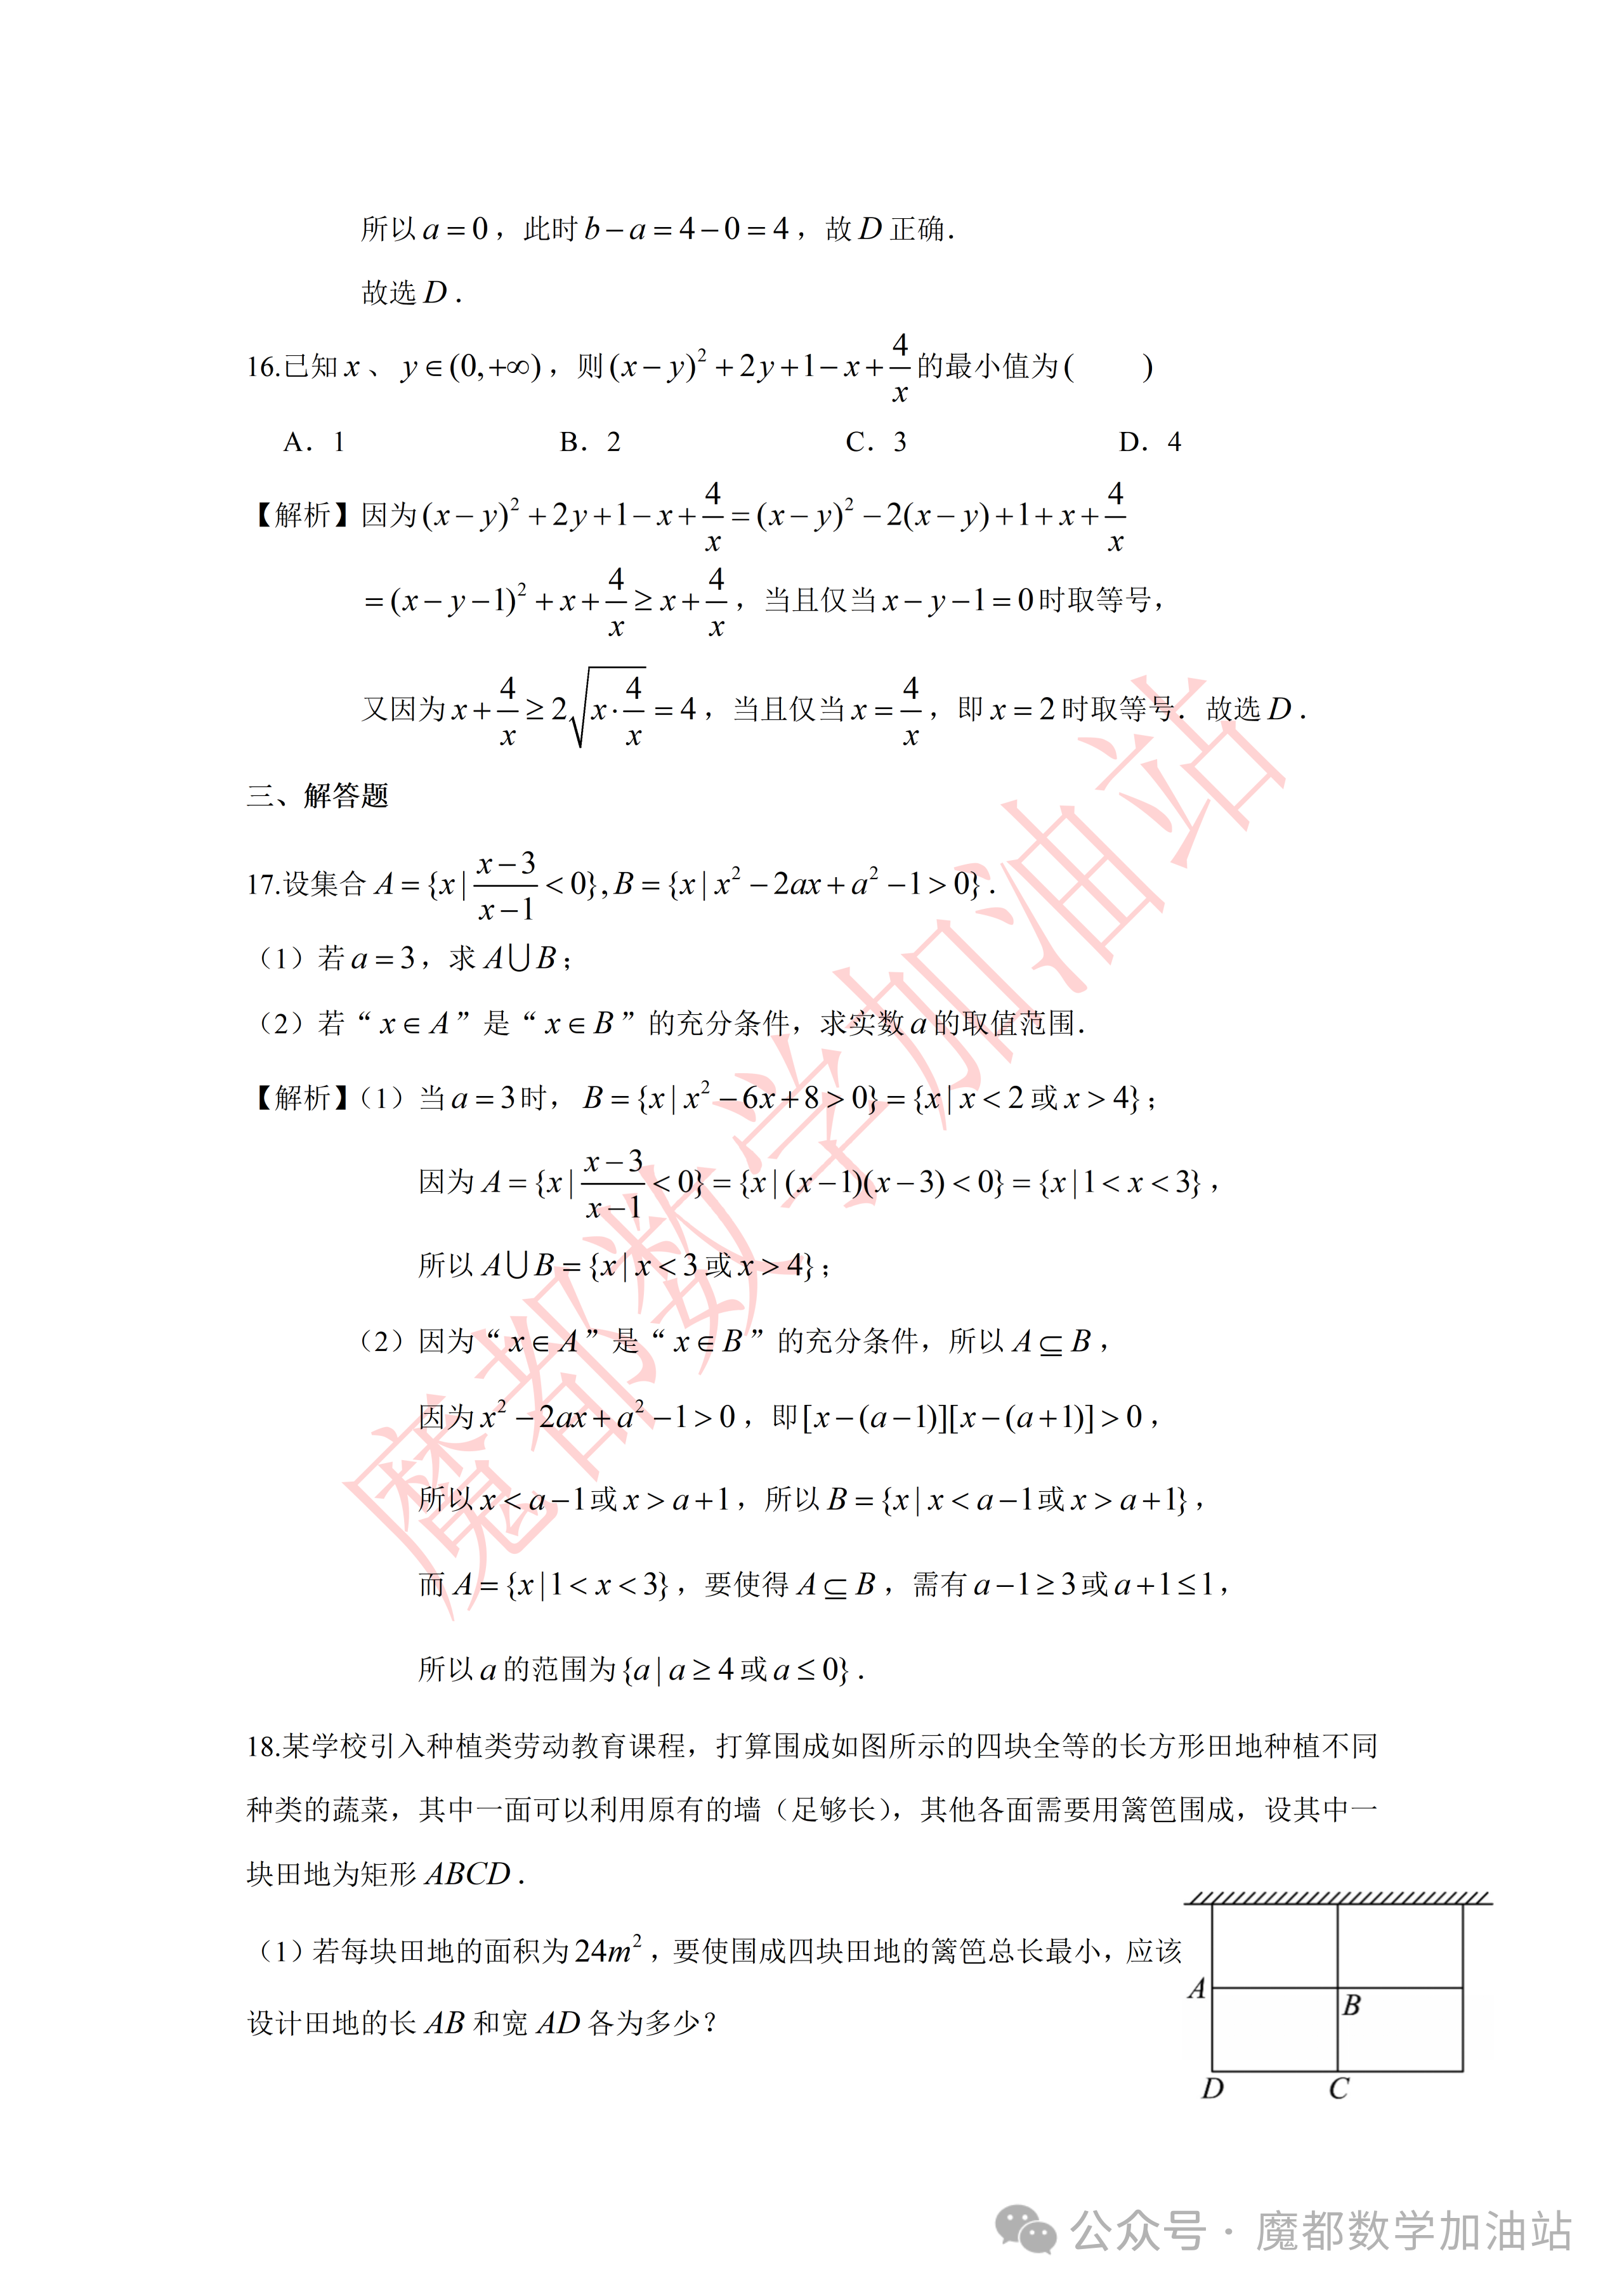
\includegraphics[width=.33\linewidth,trim=1866bp 220bp 210bp 2960bp,clip]{../原图/高一46_交附闵行_国庆作业3/06.png}
\end{center}

\begin{enumerate}[label=(\arabic*)]
\item 若每块田地的面积为 $24\,\text{m}^2$，要使围成四块田地的篱笆总长最小，应该设计田地的长 $AB$ 和宽 $AD$ 各为多少？
\item 现有 $40\,\text{m}$ 长的篱笆，要使每块田地的面积最大，应该设计田地的长 $AB$ 和宽 $AD$ 各为多少？
\end{enumerate}

\ifanswer
\solbegin
\stepm{(1)}{设 $AB$ 长为 $x\,\text{m}$，$AD$ 宽为 $y\,\text{m}$，由题意得 $xy=24$，篱笆总长为 $4x+6y$，}
\step{$4x+6y\geqslant2\sqrt{4x\cdot6y}=2\sqrt{24xy}=48$，}
\step{当且仅当 $4x=6y$ 时取等号，解得 $x=6$，$y=4$，}
\step{所以田地的长 $AB$ 为 $6\,\text{m}$，宽 $AD$ 为 $4\,\text{m}$.}
\stepm{(2)}{设 $AB$ 长为 $a\,\text{m}$，$AD$ 宽为 $b\,\text{m}$，由篱笆总长 $4a+6b=40$，即 $2a+3b=20$，}
\step{将 $a=\dfrac{20-3b}{2}$ 代入每块田地面积 $ab$，得 $ab=\dfrac12b(20-3b)=-\dfrac32b^2+10b$，}
\step{当 $b=\dfrac{10}{3}$ 时，$ab$ 最大，此时 $a=5$，}
\step{所以田地的长 $AB$ 为 $5\,\text{m}$，宽 $AD$ 为 $\dfrac{10}{3}\,\text{m}$.}
\solend
\fi

\ansspace[8]

\item 已知 $x_1$、$x_2$ 是一元二次方程 $4kx^2-4kx+k+1=0$ 的两个不等实数根.
\begin{enumerate}[label=(\arabic*)]
\item 若 $x_1$、$x_2$ 均为正根，求实数 $k$ 的取值范围；
\item 求使 $\dfrac{x_1}{x_2}+\dfrac{x_2}{x_1}-2$ 的值为整数 $k$ 的整数值.
\end{enumerate}

\ifanswer
\solbegin
\stepm{(1)}{由题意，$x_1$、$x_2$ 是方程 $4kx^2-4kx+k+1=0$ 的两个不等实数根，}
\step{故 $k\neq0$，$\Delta=(-4k)^2-16k(k+1)>0$，得 $-16k>0$，所以 $k<0$，}
\step{又 $x_1+x_2=1$，$x_1x_2=\dfrac{k+1}{4k}>0$，得 $k+1<0$，}
\step{所以 $k$ 的取值范围为 $(-\infty,-1)$.}
\stepm{(2)}{由题意，}
\step{$\dfrac{x_1}{x_2}+\dfrac{x_2}{x_1}-2
=\dfrac{x_1^2+x_2^2-2x_1x_2}{x_1x_2}
=\dfrac{(x_1+x_2)^2-4x_1x_2}{x_1x_2}$，}
\step{又 $x_1+x_2=1$，$x_1x_2=\dfrac{k+1}{4k}$，}
\step{则 $\dfrac{x_1}{x_2}+\dfrac{x_2}{x_1}-2=-\dfrac4{k+1}$，}
\step{由于 $-\dfrac4{k+1}$ 为整数，故 $k+1$ 只能取 $\pm1$、$\pm2$、$\pm4$，又 $k<-1$，}
\step{所以整数 $k$ 的值为 $-2$、$-3$、$-5$.}
\solend
\fi

\ansspace[8]

\item 已知 $a>0$，$b>0$，且 $2a+3b=3$.
\begin{enumerate}[label=(\arabic*)]
\item 求 $ab$ 的最大值；
\item 求 $a-\dfrac1{6b}$ 的最大值；
\item 求 $\dfrac2a+\dfrac3{b+1}$ 的最小值.
\end{enumerate}

\ifanswer
\solbegin
\stepm{(1)}{由 $2a+3b=3$，得 $3=2a+3b\geqslant2\sqrt{6ab}$，}
\step{所以 $ab\leqslant\dfrac38$，当且仅当 $2a=3b=\dfrac32$ 时取等号，}
\step{故 $ab$ 的最大值为 $\dfrac38$.}
\stepm{(2)}{由 $2a+3b=3$，得 $a=\dfrac32-\dfrac32b$，}
\step{则 $a-\dfrac1{6b}=\dfrac32-\dfrac32b-\dfrac1{6b}$，}
\step{由基本不等式，$\dfrac32b+\dfrac1{6b}\geqslant2\sqrt{\dfrac32b\cdot\dfrac1{6b}}=1$，}
\step{当且仅当 $\dfrac32b=\dfrac1{6b}$，即 $b=\dfrac13$、$a=1$ 时取等号，}
\step{所以 $a-\dfrac1{6b}$ 的最大值为 $\dfrac12$.}
\stepm{(3)}{由 $2a+3b=3$，得 $2a+3(b+1)=6$，}
\step{$\dfrac2a+\dfrac3{b+1}
=\dfrac16\left(2a+3(b+1)\right)\left(\dfrac2a+\dfrac3{b+1}\right)$}
\step{$=\dfrac16\left(13+\dfrac{6(b+1)}a+\dfrac{6a}{b+1}\right)
\geqslant\dfrac16\left(13+2\sqrt{\dfrac{6(b+1)}a\cdot\dfrac{6a}{b+1}}\right)=\dfrac{25}{6}$，}
\step{当且仅当 $a=b+1$，即 $a=\dfrac65$、$b=\dfrac15$ 时取等号，}
\step{所以 $\dfrac2a+\dfrac3{b+1}$ 的最小值为 $\dfrac{25}{6}$.}
\solend
\fi

\ansspace[8]

\item 已知 $U=\R$ 为全集，集合 $A=\{s^2+3t^2\mid s,t\in U\}$.
\begin{enumerate}[label=(\arabic*)]
\item 设 $U=\{1,3,5\}$，求集合 $A$ 的元素个数；
\item 设 $U=\Z$，证明：若 $x\in A$，则 $7x\in A$；
\item 设 $U=\R$，$x$、$y\in A$，且 $x=m^2+3n^2$，$y=p^2+3q^2$，若 $mp-3nq=\sqrt3$，求 $x+y+mq+np$ 的最小值.
\end{enumerate}

\ifanswer
\solbegin
\stepm{(1)}{当 $s=1$，$t=1$ 时，$s^2+3t^2=1+3=4$；}
\step{当 $s=1$，$t=3$ 时，$s^2+3t^2=1+27=28$；}
\step{当 $s=1$，$t=5$ 时，$s^2+3t^2=1+75=76$；}
\step{当 $s=3$，$t=1$ 时，$s^2+3t^2=9+3=12$；}
\step{当 $s=3$，$t=3$ 时，$s^2+3t^2=9+27=36$；}
\step{当 $s=3$，$t=5$ 时，$s^2+3t^2=9+75=84$；}
\step{当 $s=5$，$t=1$ 时，$s^2+3t^2=25+3=28$；}
\step{当 $s=5$，$t=3$ 时，$s^2+3t^2=25+27=52$；}
\step{当 $s=5$，$t=5$ 时，$s^2+3t^2=25+75=100$，}
\step{所以 $A=\{4,12,28,36,52,76,84,100\}$，有 $8$ 个元素.}
\stepm{(2)}{因为 $U=\Z$，$x\in A$，设 $x=s^2+3t^2$，}
\step{则 $7x=7(s^2+3t^2)=(2s+3t)^2+3(s-2t)^2\in A$，}
\step{所以 $7x\in A$.}
\stepm{(3)}{因为 $x=m^2+3n^2$，$y=p^2+3q^2$，}
\step{$xy=(m^2+3n^2)(p^2+3q^2)=3(mq+np)^2+(mp-3nq)^2$，}
\step{设 $mq+np=b$，则 $xy=3b^2+3$，所以 $y=\dfrac{3b^2+3}{x}$，}
\step{于是 $x+y+mq+np=x+\dfrac{3b^2+3}{x}+b\geqslant2\sqrt{3b^2+3}+b$，}
\step{设 $2\sqrt{3b^2+3}+b=t$，整理得 $11b^2+2bt+12-t^2=0$，}
\step{判别式法，$\Delta=4t^2-44(12-t^2)\geqslant0$，得 $t\geqslant\sqrt{11}$，}
\step{即 $(x+y+mq+np)_{\min}=\sqrt{11}$，所以 $x+y+mq+np$ 的最小值为 $\sqrt{11}$.}
\solend
\fi

\ansspace*[10]

\end{enumerate}

\end{document}
"
%
% 原始材料：微信公众号“魔都数学加油站”，作者破晓，2026-10-02 17:56 发布。
% 原文标题：“27学年高一46——2026-2027你那上海市交附闵行高一上国庆作业3”
% （公众号标题中的“你那”照录，系原文标题字样）；原文链接：
% http://mp.weixin.qq.com/s?__biz=Mzg4ODU1ODMxOQ==&mid=2247591657&idx=3&sn=a894d1a16611283a61b3eaba32a3f24c&chksm=cee83366c6a55381b370069f84ef63d20251f94608bb37cc4ec2d66227401bd147f4f6bd8256&scene=126&sessionid=1790935402&subscene=7&clicktime=1790937618&enterid=1790937618#rd
% 正文为 9 张 PNG 页，按页序读取原图；第 01、02、07 页 4762×6735，
% 第 03—06、08、09 页 2560×3620。卷面标题照原卷印作“2026-2027 年交附闵行高一上国庆作业 3”。
% 原文从第 3 题起，题号照原卷保留；正文为讲评版，答案、解析依原卷顺序录入。
% 水印及页脚公众号标识不录入。卷面插图直接裁取对应原图页，不另制图片文件。
%
% 与原卷的排版差异：
%   ① 原卷按“一、填空题”“二、选择题”“三、解答题”分节，本稿沿用原节与原题号，
%      只改排为全稿统一的大节样式；
%   ② 原卷答案与解析依页面位置分布，本稿按 common.sty 统一置于答案版；
%   ③ 原卷副标题未印，本稿按“知识模块”口径标作“集合与常用逻辑用语、不等式”。
%
% 原卷存疑一处（照抄未改，见第 12 题题干及解析处注释）：
%   第 12 题题干同时给出 x∈Z，却称不等式组有“50 个不等的实数解”；解析按整数根计数。
%   此处题干与解析的原文不一致，本稿均照录。
% 第 17 题曾疑似有常数项不一致：复核原图题干为 a^2-1，a=3 时常数项确为 8，
% 与解析相符；不将其记作原卷错误。
%
\documentclass[a4paper,11pt]{article}
\usepackage{common}

\begin{document}

\examtitlest[3]{2026--2027 年交附闵行高一上国庆作业 3}{集合与常用逻辑用语、不等式}

\bigsec{一、填空题}

\begin{enumerate}
\setcounter{enumi}{2}

\item 不等式 $\dfrac{x^2-10}{x+2}\geqslant1$ 的解集为\blankline[4.4em].

\ifanswer
\ans{$\{x\mid-3\leqslant x<-2\text{ 或 }x\geqslant4\}$}
\solbegin
\step{不等式 $\dfrac{x^2-10}{x+2}\geqslant1$，移项得 $\dfrac{x^2-10}{x+2}-1\geqslant0$，}
\step{通分得 $\dfrac{x^2-x-12}{x+2}\geqslant0$，即 $\dfrac{(x-4)(x+3)}{x+2}\geqslant0$，}
\step{解得 $-3\leqslant x<-2$ 或 $x\geqslant4$，}
\step{故不等式的解集为 $\{x\mid-3\leqslant x<-2\text{ 或 }x\geqslant4\}$.}
\solend
\fi

\item $|x-3|+|x-5|\geqslant2$，当等号成立时，$x$ 的范围是\blankline[4.4em].

\ifanswer
\ans{$[3,5]$}
\fi

\item 若直角三角形斜边长等于 $4\sqrt2\,\text{cm}$，则直角三角形面积的最大值为\blankline[4.4em].

\ifanswer
\solbegin
\step{设 $Rt\triangle ABC$ 中，$C=90^\circ$，则 $c=\sqrt{a^2+b^2}=4\sqrt2$，所以 $a^2+b^2=32$，}
\step{由基本不等式得 $a^2+b^2\geqslant2ab$，当且仅当 $a=b=4$ 时取等号，}
\step{所以 $\triangle ABC$ 的面积 $S=\dfrac12ab\leqslant8$，}
\step{当且仅当 $a=b=4$ 时，$\triangle ABC$ 的面积最大值为 $8$.}
\solend
\fi

\item 不等式 $(x-1)(2-x)>0$ 的解集为\blankline[4.4em].

\ifanswer
\solbegin
\step{$(x-1)(2-x)>0\Rightarrow(x-1)(x-2)<0$，}
\step{故不等式的解集为 $\{x\mid1<x<2\}$.}
\solend
\fi

\item 已知集合 $A=\{1,2\}$，$B=\{x\mid x^2-2mx+m=0\}$，$A\cup B=A$，则实数 $m$ 的取值范围为\blankline[4.4em].

\ifanswer
\solbegin
\step{因为 $A\cup B=A$，所以 $B\subseteq A$，}
\step{当 $B=\varnothing$ 时，$\Delta=(-2m)^2-4m<0$，解得 $0<m<1$，}
\step{当 $B$ 为单元素集时，$\Delta=0$，解得 $m=0$ 或 $m=1$，}
\step{当 $m=0$ 时，方程 $x^2=0$，解得 $x=0$，此时 $B=\{0\}$，不满足 $B\subseteq A$；}
\step{当 $m=1$ 时，方程 $x^2-2x+1=0$，解得 $x=1$，此时 $B=\{1\}$，满足 $B\subseteq A$；}
\step{当 $B=\{1,2\}$ 时，由韦达定理得 $1+2=2m$，$1\times2=m$，无解，}
\step{综上所述，实数 $m$ 的取值范围为 $\{m\mid0<m\leqslant1\}$.}
\solend
\fi

\item 设 $a$、$b$、$c\in\R^+$，若 $a+b+c=1$，则 $\dfrac1a+\dfrac1b+\dfrac1c\geqslant$\blankline[4.4em].

\ifanswer
\solbegin
\step{因为 $a$、$b$、$c\in\R^+$，且 $a+b+c=1$，}
\step{所以 $\dfrac1a+\dfrac1b+\dfrac1c=(a+b+c)\left(\dfrac1a+\dfrac1b+\dfrac1c\right)$}
\step{$=3+\dfrac ab+\dfrac ba+\dfrac ac+\dfrac ca+\dfrac bc+\dfrac cb$，}
\step{由基本不等式得 $\dfrac ab+\dfrac ba\geqslant2$，$\dfrac ac+\dfrac ca\geqslant2$，$\dfrac bc+\dfrac cb\geqslant2$，}
\step{所以 $\dfrac1a+\dfrac1b+\dfrac1c\geqslant9$，当且仅当 $a=b=c=\dfrac13$ 时取等号，}
\step{所以 $\dfrac1a+\dfrac1b+\dfrac1c$ 的最小值为 $9$.}
\solend
\fi

\item 已知 $-1\leqslant x+y\leqslant2$，$-2\leqslant x-y\leqslant1$，则 $x-2y$ 的范围为\blankline[4.4em].

\ifanswer
\solbegin
\step{设 $x-2y=m(x+y)+n(x-y)$，}
\step{则 $x-2y=(m+n)x+(m-n)y$，所以 $m+n=1$，$m-n=-2$，}
\step{解得 $m=-\dfrac12$，$n=\dfrac32$，}
\step{所以 $x-2y=-\dfrac12(x+y)+\dfrac32(x-y)$，}
\step{因为 $-1\leqslant x+y\leqslant2$，$-2\leqslant x-y\leqslant1$，}
\step{所以 $-4\leqslant x-2y\leqslant2$，即 $x-2y$ 的范围为 $[-4,2]$.}
\solend
\fi

\item 设集合 $A=\{1,2,m\}$，其中 $m$ 为实数，令 $B=\{a^2\mid a\in A\}$，$C=A\cup B$. 若 $C$ 中所有元素之和为 $6$，则 $C$ 中的所有元素之积为\blankline[4.4em].

\ifanswer
\solbegin
\step{因为 $A=\{1,2,m\}$，所以 $B=\{a^2\mid a\in A\}=\{1,4,m^2\}$，$m\neq1$，$m\neq2$，}
\step{又 $C=A\cup B$，所以 $1\in C$，$4\in C$，$m^2\in C$，}
\step{若 $m^2=1$，则 $m=-1$ 或 $m=1$（舍），当 $m=-1$ 时，$C=\{1,2,4,-1\}$，$C$ 中所有元素之和为 $6$，}
\step{此时 $C$ 中所有元素之积为 $-8$；}
\step{若 $m^2=2$，则 $m=-\sqrt2$ 或 $m=\sqrt2$，$C$ 中所有元素之和不符合题意；}
\step{若 $m^2=4$，则 $m=-2$ 或 $m=2$，此时 $C=\{1,2,4,-2\}$ 或 $C=\{1,2,4\}$，所有元素之和不符合题意；}
\step{若 $m^2\neq1$，$m^2\neq2$，$m^2\neq4$，则 $C=\{1,2,4,m,m^2\}$，}
\step{所以 $1+2+4+m+m^2=6$，即 $m^2+m+1=0$，无解，}
\step{综上所述，$C$ 中所有元素之积为 $-8$.}
\solend
\fi

\item 若对任意实数 $x>0$，$y>0$，不等式 $x+\sqrt{xy}\leqslant a(x+y)$ 恒成立，则实数 $a$ 的最小值为\blankline[4.4em].

\ifanswer
\solbegin
\step{由不等式 $x+\sqrt{xy}\leqslant a(x+y)$ 对任意实数 $x>0$，$y>0$ 恒成立，}
\step{得 $a\geqslant\dfrac{x+\sqrt{xy}}{x+y}$，}
\step{设 $\sqrt{\dfrac yx}=t>0$，则 $a\geqslant\dfrac{1+t}{1+t^2}$，}
\step{$\dfrac{1+t}{1+t^2}\leqslant\dfrac{\sqrt2+1}{2}$，当且仅当 $t=\sqrt2-1$ 时取等号，}
\step{所以实数 $a$ 的最小值为 $\dfrac{\sqrt2+1}{2}$.}
\solend
\fi

% 注：原卷题干给出 x∈Z，却写“实数解”；解析按整数解计数，题干与解析不一致，照录未改。
\item 若关于 $x$ 的不等式组
$\begin{cases}x^2-3mx\geqslant4m^2\\-20<x<120\end{cases}$（$x\in\Z,m>0$）恰有 $50$ 个不等的实数解，则 $m$ 的取值范围为\blankline[4.4em]（结果用区间表示）.

\ifanswer
\solbegin
\step{由 $x^2-3mx\geqslant4m^2$ 以及 $m>0$，解得 $x\leqslant-m$ 或 $x\geqslant4m$，}
\step{由原不等式组恰有 $50$ 个不等的实数解，可画出如下解集区间：}
\begin{center}
% 原图第 4 页数轴图直接裁取。
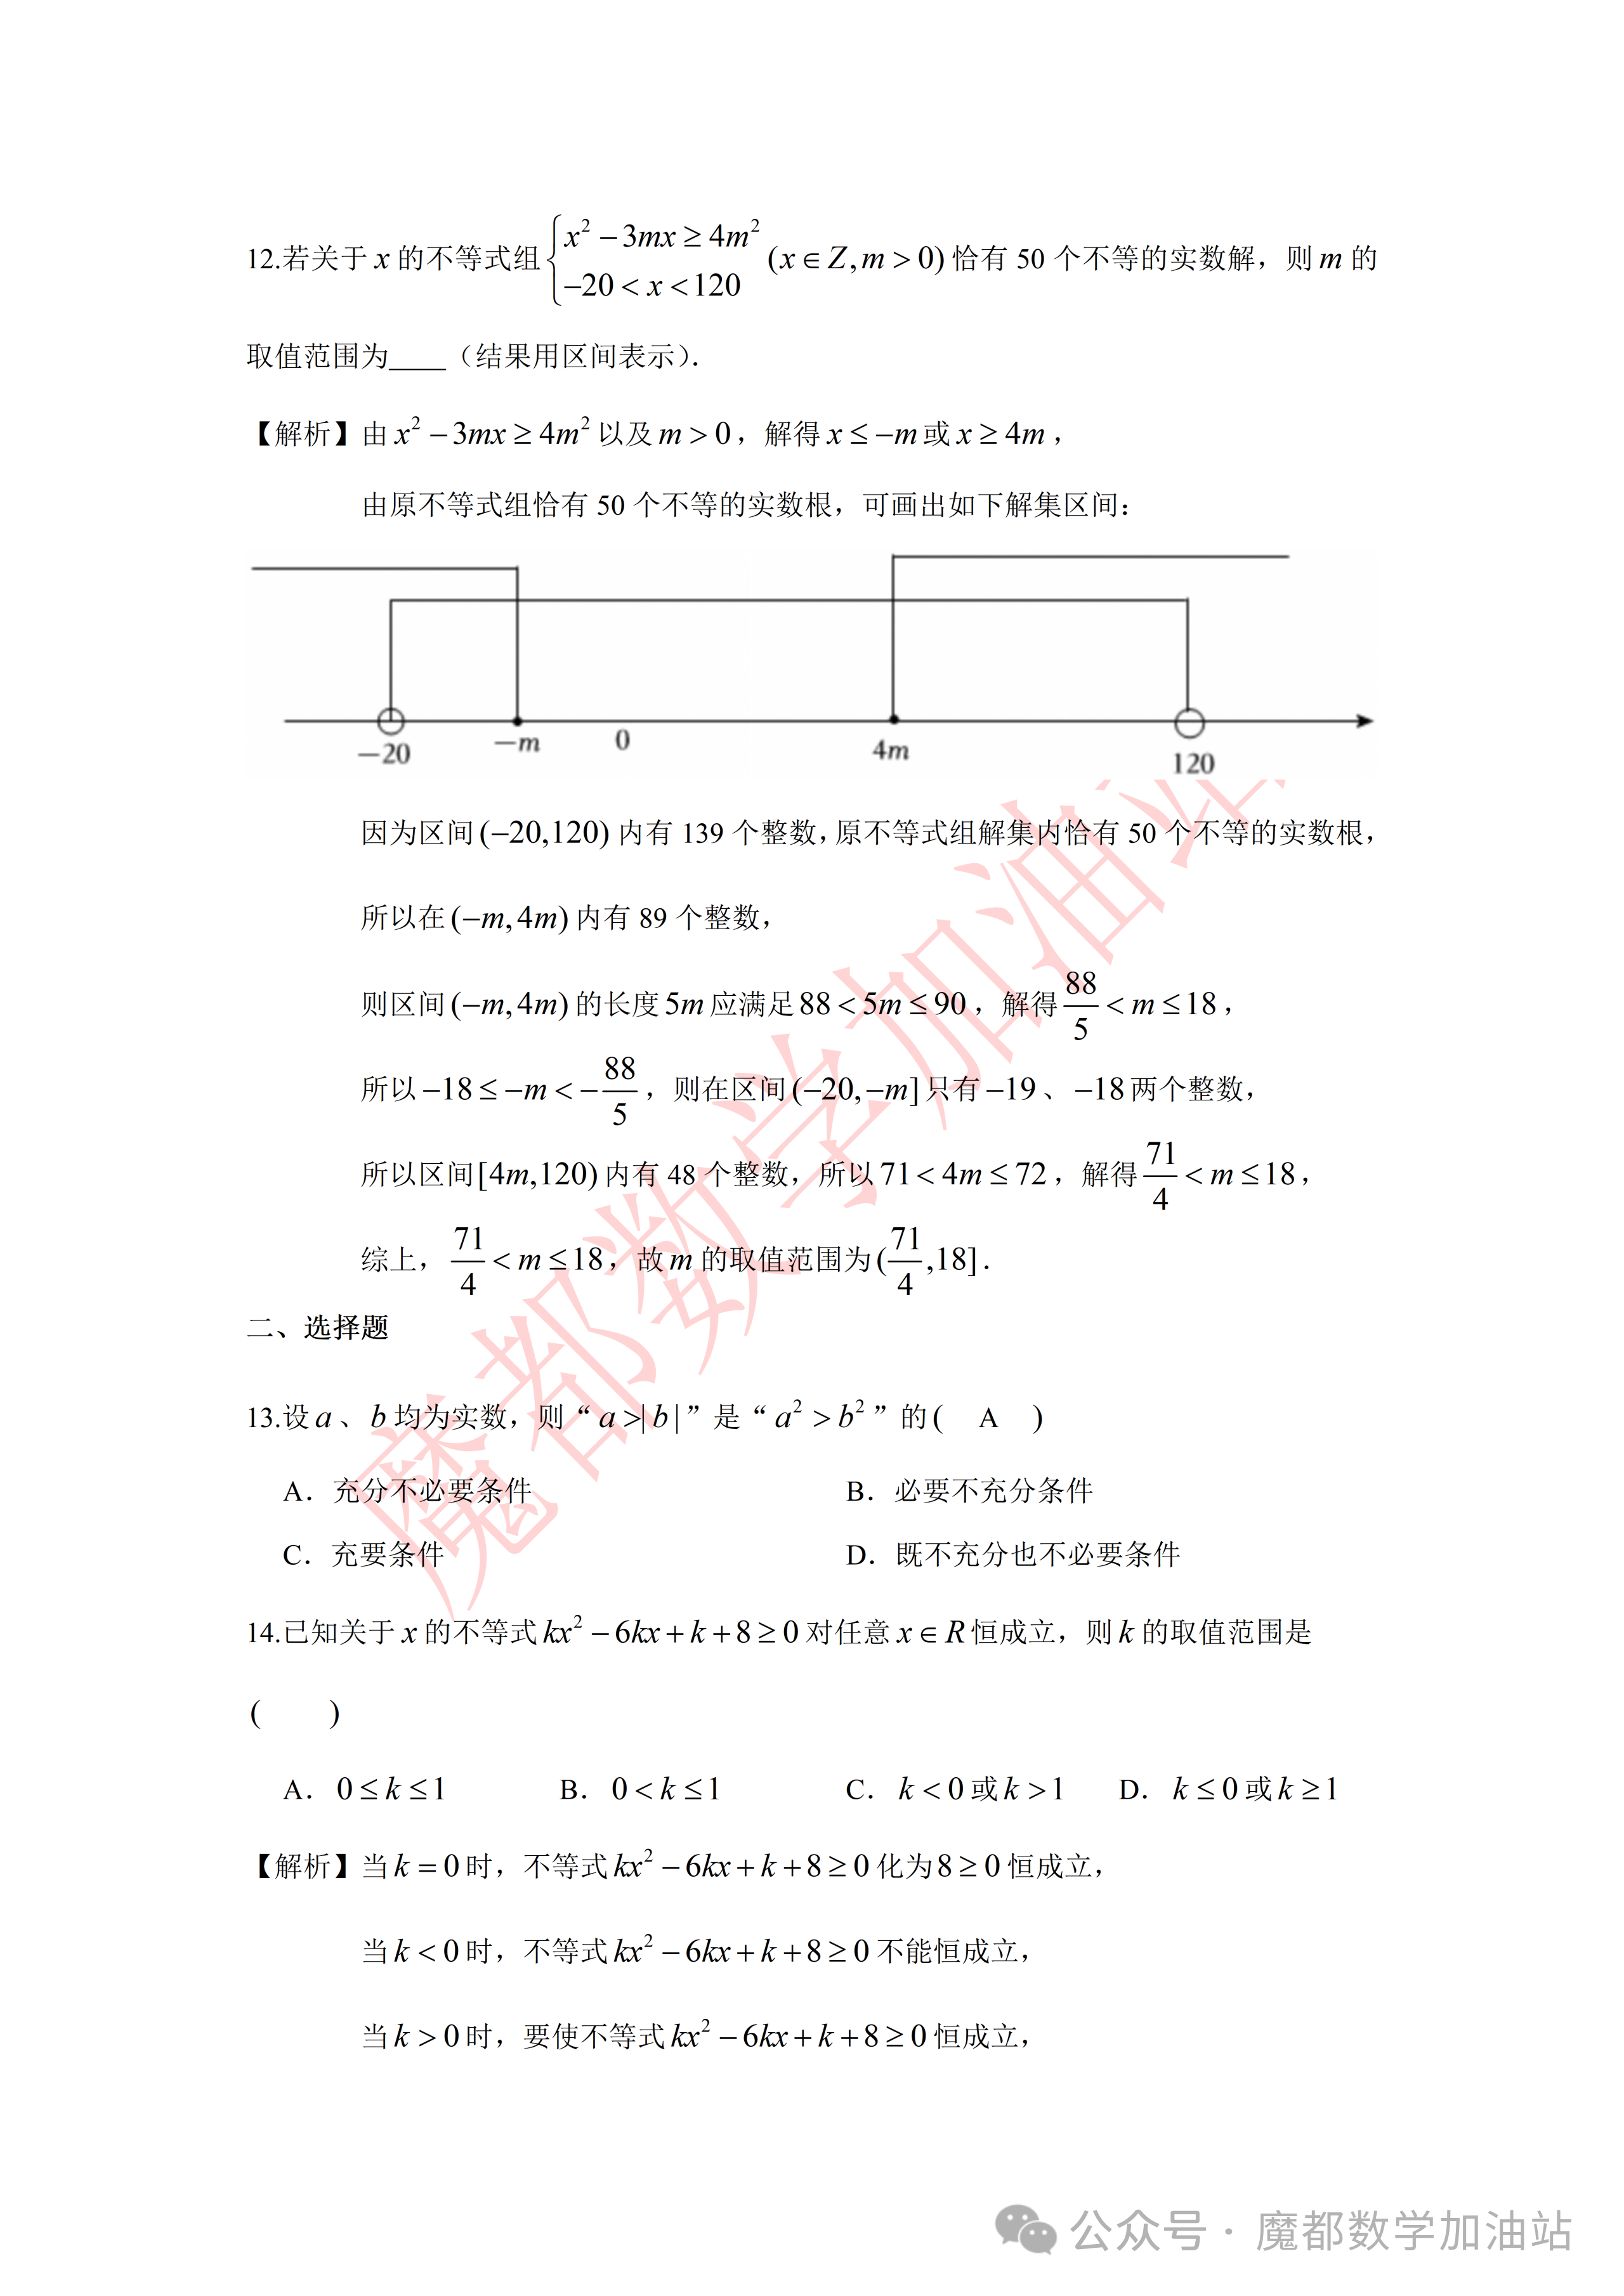
\includegraphics[width=.88\linewidth,trim=400bp 2410bp 320bp 860bp,clip]{../原图/高一46_交附闵行_国庆作业3/04.png}
\end{center}
\step{因为区间 $(-20,120)$ 内有 $139$ 个整数，原不等式组解集内有 $50$ 个不等的整数根，}
\step{所以在区间 $(-m,4m)$ 内有 $89$ 个整数，}
\step{则区间 $(-m,4m)$ 的长度 $5m$ 应满足 $88<5m\leqslant90$，解得 $\dfrac{88}{5}<m\leqslant18$，}
% 注：原卷题干称“实数解”，本行及后文按原卷解析照录为整数根计数。
\step{所以 $-18\leqslant-m<-\dfrac{88}{5}$，则在区间 $(-20,-m]$ 内有 $-19$、$-18$ 两个整数，}
\step{所以区间 $[4m,120)$ 内有 $48$ 个整数，}
\step{则 $71<4m\leqslant72$，解得 $\dfrac{71}{4}<m\leqslant18$，}
\step{综上，$\dfrac{71}{4}<m\leqslant18$，故 $m$ 的取值范围为 $\left(\dfrac{71}{4},18\right]$.}
\solend
\fi

\end{enumerate}

\bigsec{二、选择题}

\begin{enumerate}
\setcounter{enumi}{12}

\item 设 $a$、$b$ 均为实数，则“$a>|b|$”是“$a^2>b^2$”的\mbox{（\quad）}

\keepwithprev
A. 充分不必要条件\qquad B. 必要不充分条件

C. 充要条件\qquad\qquad D. 既不充分也不必要条件

\ans{$A$}

\item 已知关于 $x$ 的不等式 $kx^2-6kx+k+8\geqslant0$ 对任意 $x\in\R$ 恒成立，则 $k$ 的取值范围是\mbox{（\quad）}

\keepwithprev
A. $0\leqslant k\leqslant1$\qquad B. $0<k\leqslant1$

C. $k<0$ 或 $k>1$\qquad D. $k\leqslant0$ 或 $k\geqslant1$

\ans{$A$}

\ifanswer
\solbegin
\step{当 $k=0$ 时，不等式 $kx^2-6kx+k+8\geqslant0$ 化为 $8\geqslant0$ 恒成立，}
\step{当 $k<0$ 时，不等式 $kx^2-6kx+k+8\geqslant0$ 不能恒成立，}
\step{当 $k>0$ 时，要使不等式 $kx^2-6kx+k+8\geqslant0$ 恒成立，}
\step{需 $\Delta=36k^2-4(k^2+8k)\leqslant0$，解得 $0\leqslant k\leqslant1$，故选 $A$.}
\solend
\fi

\item 已知关于 $x$ 的不等式 $a\leqslant\dfrac34x^2-3x+4\leqslant b$，下列结论正确的是\mbox{（\quad）}

\keepwithprev
A. 当 $a<b<1$ 时，不等式 $a\leqslant\dfrac34x^2-3x+4\leqslant b$ 的解集非空

B. 当 $a=2$ 时，不等式 $a\leqslant\dfrac34x^2-3x+4\leqslant b$ 的解集可以为 $\{x\mid c\leqslant x\leqslant d\}$ 的形式

C. 不等式 $a\leqslant\dfrac34x^2-3x+4\leqslant b$ 的解集恰好为 $\{x\mid a\leqslant x\leqslant b\}$，那么 $b=\dfrac43$

D. 不等式 $a\leqslant\dfrac34x^2-3x+4\leqslant b$ 的解集恰好为 $\{x\mid a\leqslant x\leqslant b\}$，那么 $b-a=4$

\ans{$D$}

\ifanswer
\solbegin
\step{由 $\dfrac34x^2-3x+4\leqslant b$，得 $3x^2-12x+16-4b\leqslant0$，又 $b<1$，}
\step{所以 $\Delta=144-12(16-4b)=48(b-1)<0$，从而不等式无解，故 $A$ 错误；}
\step{在同一平面直角坐标系中作出函数 $y=\dfrac34x^2-3x+4=\dfrac34(x-2)^2+1$ 的图象及直线 $y=a$ 和 $y=b$，如图所示.}
\begin{center}
% 原图第 5 页解析配图直接裁取。
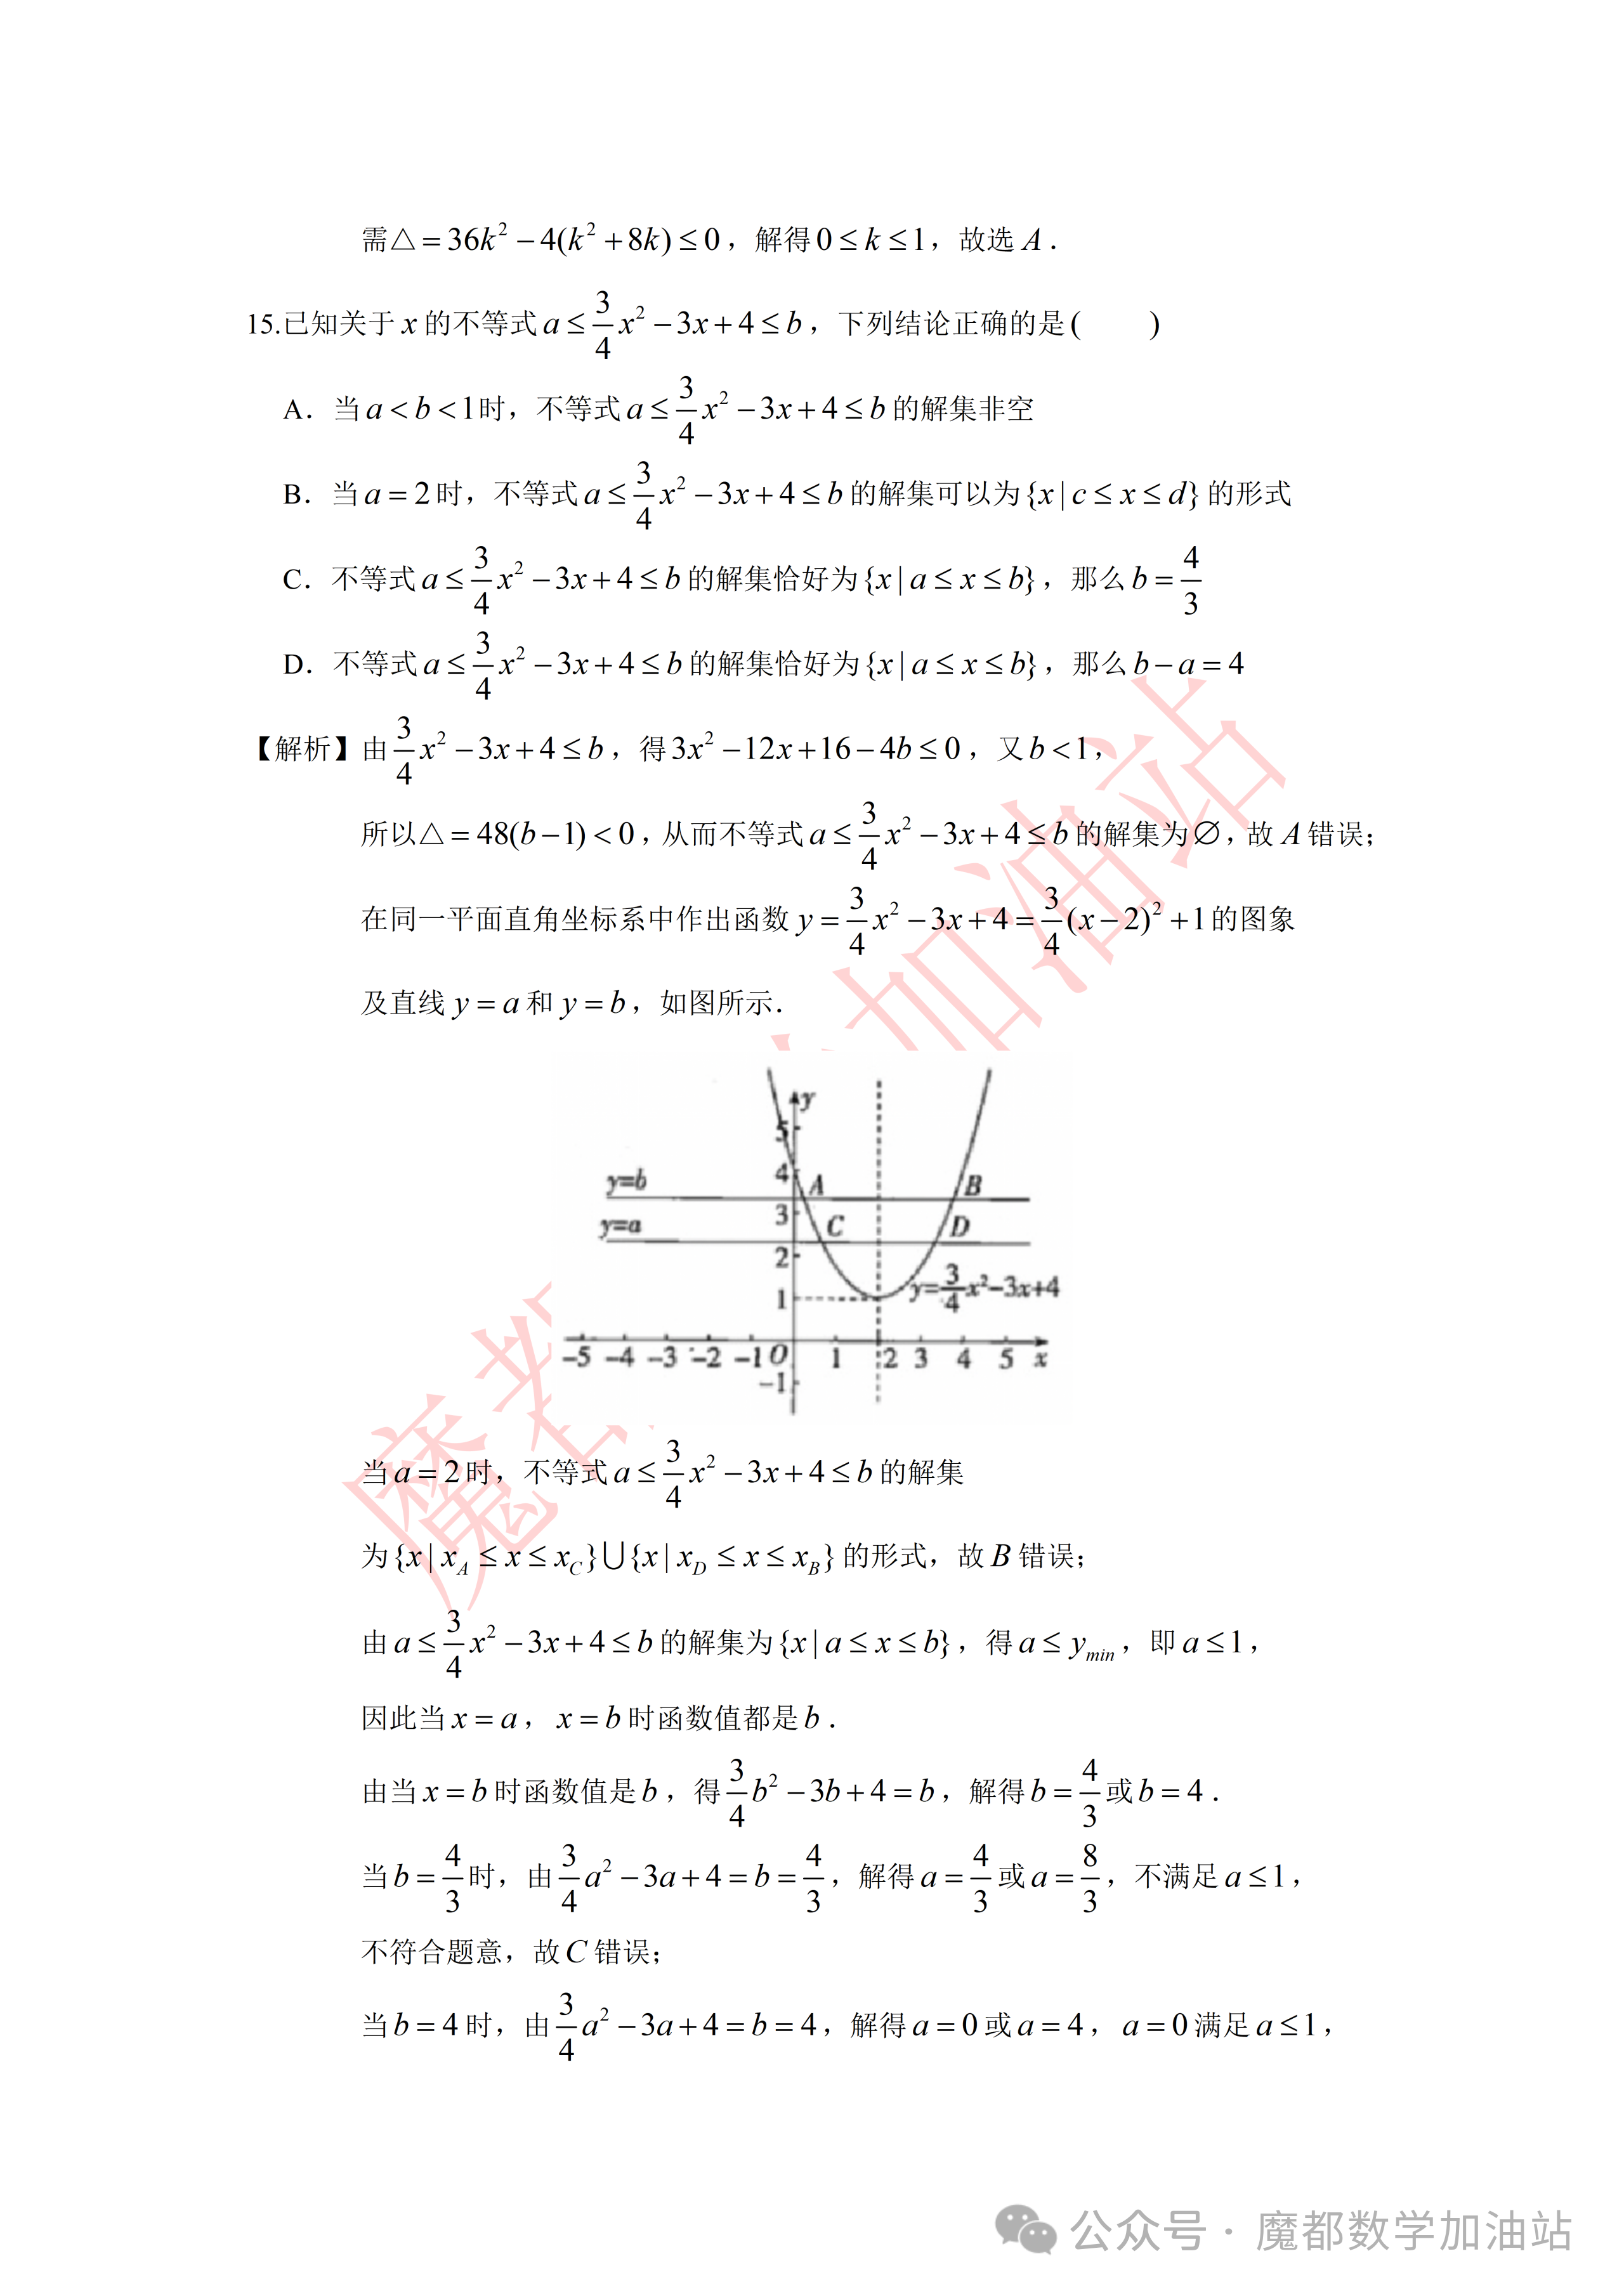
\includegraphics[width=.55\linewidth,trim=900bp 1400bp 760bp 1680bp,clip]{../原图/高一46_交附闵行_国庆作业3/05.png}
\end{center}
\step{当 $a=2$ 时，不等式 $a\leqslant\dfrac34x^2-3x+4\leqslant b$ 的解集为
$\{x\mid x_A\leqslant x\leqslant x_C\}\cup\{x\mid x_D\leqslant x\leqslant x_B\}$ 的形式，故 $B$ 错误；}
\step{由 $a\leqslant\dfrac34x^2-3x+4\leqslant b$ 的解集恰好为 $\{x\mid a\leqslant x\leqslant b\}$ 的形式，得 $a\leqslant y_{\min}$，即 $a\leqslant1$，}
\step{因为当 $x=a$、$x=b$ 时函数值都是 $b$，当 $x=a$ 时，$\dfrac34a^2-3a+4=b$；当 $x=b$ 时，$\dfrac34b^2-3b+4=b$，}
\step{解得 $b=\dfrac43$ 或 $b=4$，}
\step{当 $b=\dfrac43$ 时，由 $\dfrac34a^2-3a+4=b$，解得 $a=\dfrac43$ 或 $a=\dfrac83$，不符合题意，故 $C$ 错误；}
\step{当 $b=4$ 时，由 $\dfrac34a^2-3a+4=b$，解得 $a=0$ 或 $a=4$，$a=0$ 满足 $a\leqslant1$，故 $D$ 正确；}
\step{故选 $D$.}
\solend
\fi

\item 已知 $x$、$y\in(0,+\infty)$，则 $(x-y)^2+2y+1-x+\dfrac4x$ 的最小值为\mbox{（\quad）}

\keepwithprev
A. $1$\qquad B. $2$\qquad C. $3$\qquad D. $4$

\ans{$D$}

\ifanswer
\solbegin
\step{因为 $(x-y)^2+2y+1-x+\dfrac4x=(x-y-1)^2+x+\dfrac4x$，}
\step{当且仅当 $x-y-1=0$，且 $x=\dfrac4x$ 时取等号，}
\step{又因为 $x+\dfrac4x\geqslant2\sqrt{x\cdot\dfrac4x}=4$，当且仅当 $x=2$ 时取等号，}
\step{故选 $D$.}
\solend
\fi

\end{enumerate}

\bigsec{三、解答题}

\begin{enumerate}
\setcounter{enumi}{16}

\item 设集合 $A=\left\{x\middle|\dfrac{x-3}{x-1}<0\right\}$，$B=\{x\mid x^2-2ax+a^2-1>0\}$.
\begin{enumerate}[label=(\arabic*)]
\item 若 $a=3$，求 $A\cup B$；
\item 若“$x\in A$”是“$x\in B$”的充分条件，求实数 $a$ 的取值范围.
\end{enumerate}

\ifanswer
\solbegin
% 注：原卷题干为 a^2-1，故 a=3 时常数项为 8；题干与本步一致。
\stepm{(1)}{当 $a=3$ 时，$B=\{x\mid x^2-6x+8>0\}=\{x\mid x<2\text{ 或 }x>4\}$；}
\step{因为 $A=\left\{x\middle|\dfrac{x-3}{x-1}<0\right\}=\{x\mid(x-1)(x-3)<0\}=\{x\mid1<x<3\}$，}
\step{所以 $A\cup B=\{x\mid x<2\text{ 或 }x>4\}\cup\{x\mid1<x<3\}
=\{x\mid x<3\text{ 或 }x>4\}$.}
\stepm{(2)}{因为“$x\in A$”是“$x\in B$”的充分条件，所以 $A\subseteq B$，}
\step{因 $A=\left\{x\middle|\dfrac{x-3}{x-1}<0\right\}
=\{x\mid(x-1)(x-3)<0\}=\{x\mid1<x<3\}$，}
\step{所以 $A\subseteq B=\{x\mid x<a-1\text{ 或 }x>a+1\}$，}
\step{要使 $A\subseteq B$，需有 $a-1\geqslant3$ 或 $a+1\leqslant1$，}
\step{所以 $a\geqslant4$ 或 $a\leqslant0$，故 $a$ 的取值范围为 $\{a\mid a\geqslant4\text{ 或 }a\leqslant0\}$.}
\solend
\fi

\ansspace[6]

\item 某学校引入种植类劳动教育课程，打算围成如图所示的四块全等的长方形田地种植不同种类的蔬菜，其中一面可以利用原有的墙（足够长），其他各面需要用篱笆围成，设其中一块田地为矩形 $ABCD$.

\begin{center}
% 原图第 6 页配图直接裁取。
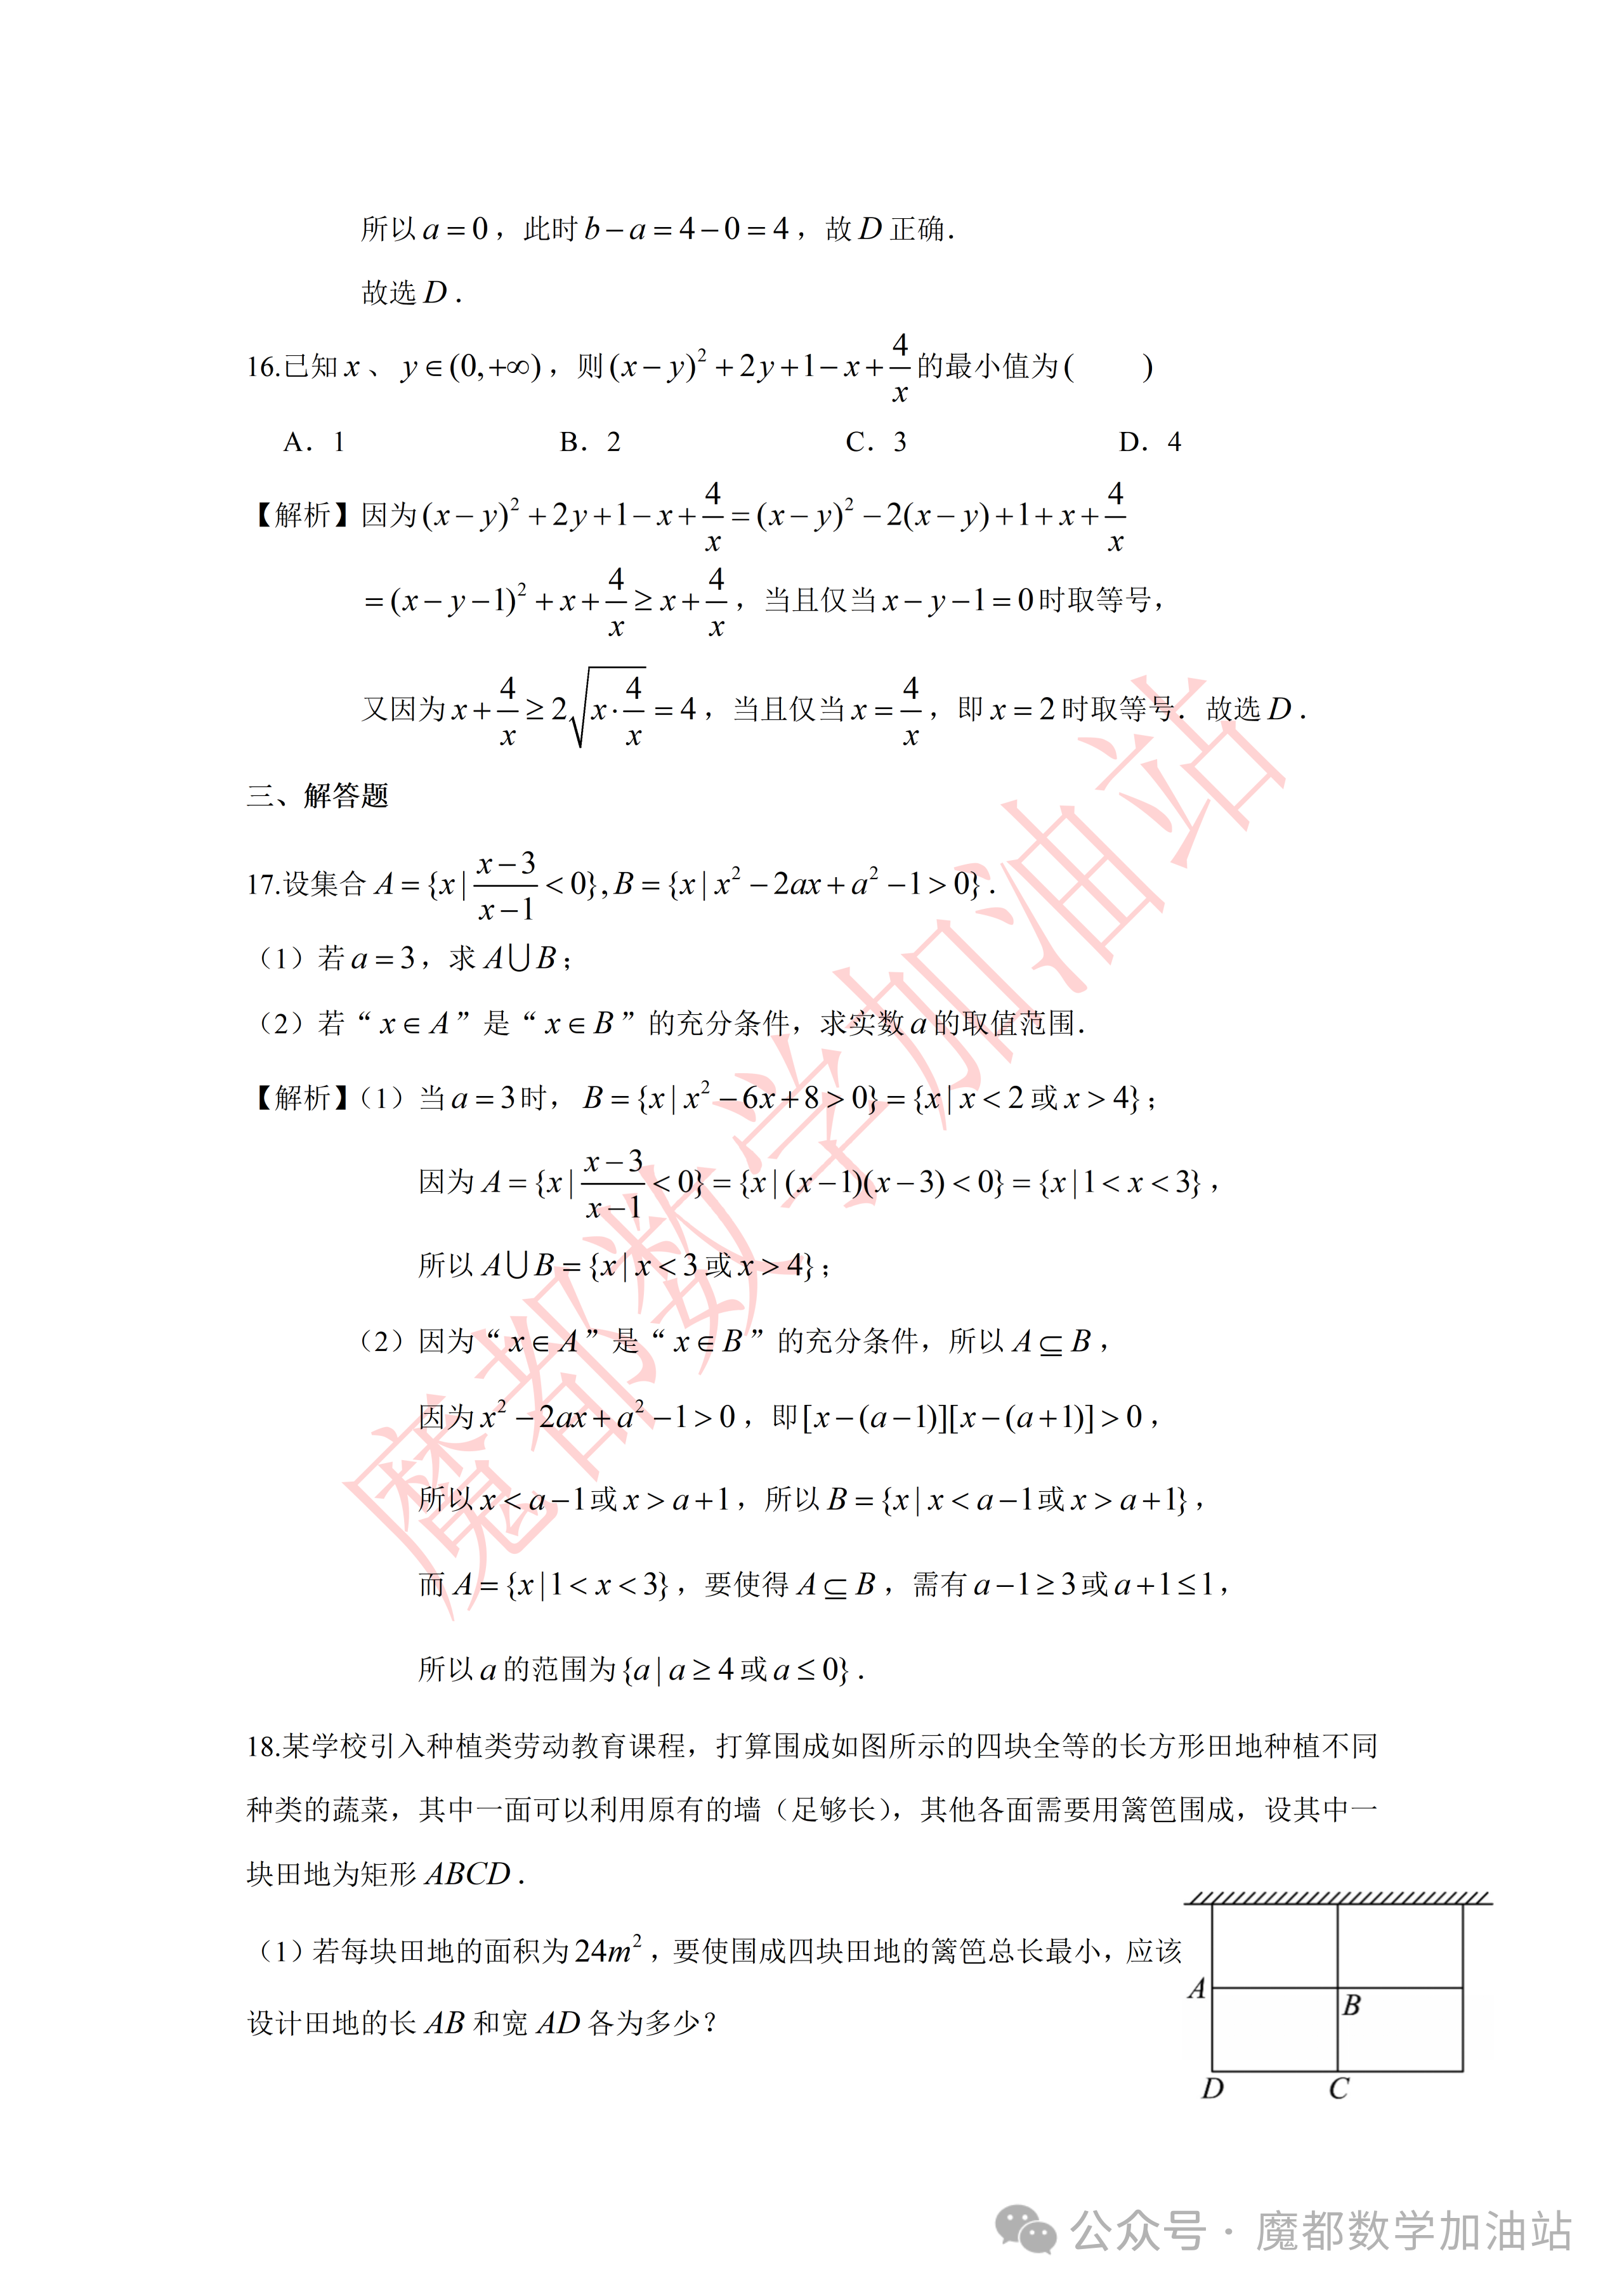
\includegraphics[width=.33\linewidth,trim=1866bp 220bp 210bp 2960bp,clip]{../原图/高一46_交附闵行_国庆作业3/06.png}
\end{center}

\begin{enumerate}[label=(\arabic*)]
\item 若每块田地的面积为 $24\,\text{m}^2$，要使围成四块田地的篱笆总长最小，应该设计田地的长 $AB$ 和宽 $AD$ 各为多少？
\item 现有 $40\,\text{m}$ 长的篱笆，要使每块田地的面积最大，应该设计田地的长 $AB$ 和宽 $AD$ 各为多少？
\end{enumerate}

\ifanswer
\solbegin
\stepm{(1)}{设 $AB$ 长为 $x\,\text{m}$，$AD$ 宽为 $y\,\text{m}$，由题意得 $xy=24$，篱笆总长为 $4x+6y$，}
\step{$4x+6y\geqslant2\sqrt{4x\cdot6y}=2\sqrt{24xy}=48$，}
\step{当且仅当 $4x=6y$ 时取等号，解得 $x=6$，$y=4$，}
\step{所以田地的长 $AB$ 为 $6\,\text{m}$，宽 $AD$ 为 $4\,\text{m}$.}
\stepm{(2)}{设 $AB$ 长为 $a\,\text{m}$，$AD$ 宽为 $b\,\text{m}$，由篱笆总长 $4a+6b=40$，即 $2a+3b=20$，}
\step{将 $a=\dfrac{20-3b}{2}$ 代入每块田地面积 $ab$，得 $ab=\dfrac12b(20-3b)=-\dfrac32b^2+10b$，}
\step{当 $b=\dfrac{10}{3}$ 时，$ab$ 最大，此时 $a=5$，}
\step{所以田地的长 $AB$ 为 $5\,\text{m}$，宽 $AD$ 为 $\dfrac{10}{3}\,\text{m}$.}
\solend
\fi

\ansspace[8]

\item 已知 $x_1$、$x_2$ 是一元二次方程 $4kx^2-4kx+k+1=0$ 的两个不等实数根.
\begin{enumerate}[label=(\arabic*)]
\item 若 $x_1$、$x_2$ 均为正根，求实数 $k$ 的取值范围；
\item 求使 $\dfrac{x_1}{x_2}+\dfrac{x_2}{x_1}-2$ 的值为整数 $k$ 的整数值.
\end{enumerate}

\ifanswer
\solbegin
\stepm{(1)}{由题意，$x_1$、$x_2$ 是方程 $4kx^2-4kx+k+1=0$ 的两个不等实数根，}
\step{故 $k\neq0$，$\Delta=(-4k)^2-16k(k+1)>0$，得 $-16k>0$，所以 $k<0$，}
\step{又 $x_1+x_2=1$，$x_1x_2=\dfrac{k+1}{4k}>0$，得 $k+1<0$，}
\step{所以 $k$ 的取值范围为 $(-\infty,-1)$.}
\stepm{(2)}{由题意，}
\step{$\dfrac{x_1}{x_2}+\dfrac{x_2}{x_1}-2
=\dfrac{x_1^2+x_2^2-2x_1x_2}{x_1x_2}
=\dfrac{(x_1+x_2)^2-4x_1x_2}{x_1x_2}$，}
\step{又 $x_1+x_2=1$，$x_1x_2=\dfrac{k+1}{4k}$，}
\step{则 $\dfrac{x_1}{x_2}+\dfrac{x_2}{x_1}-2=-\dfrac4{k+1}$，}
\step{由于 $-\dfrac4{k+1}$ 为整数，故 $k+1$ 只能取 $\pm1$、$\pm2$、$\pm4$，又 $k<-1$，}
\step{所以整数 $k$ 的值为 $-2$、$-3$、$-5$.}
\solend
\fi

\ansspace[8]

\item 已知 $a>0$，$b>0$，且 $2a+3b=3$.
\begin{enumerate}[label=(\arabic*)]
\item 求 $ab$ 的最大值；
\item 求 $a-\dfrac1{6b}$ 的最大值；
\item 求 $\dfrac2a+\dfrac3{b+1}$ 的最小值.
\end{enumerate}

\ifanswer
\solbegin
\stepm{(1)}{由 $2a+3b=3$，得 $3=2a+3b\geqslant2\sqrt{6ab}$，}
\step{所以 $ab\leqslant\dfrac38$，当且仅当 $2a=3b=\dfrac32$ 时取等号，}
\step{故 $ab$ 的最大值为 $\dfrac38$.}
\stepm{(2)}{由 $2a+3b=3$，得 $a=\dfrac32-\dfrac32b$，}
\step{则 $a-\dfrac1{6b}=\dfrac32-\dfrac32b-\dfrac1{6b}$，}
\step{由基本不等式，$\dfrac32b+\dfrac1{6b}\geqslant2\sqrt{\dfrac32b\cdot\dfrac1{6b}}=1$，}
\step{当且仅当 $\dfrac32b=\dfrac1{6b}$，即 $b=\dfrac13$、$a=1$ 时取等号，}
\step{所以 $a-\dfrac1{6b}$ 的最大值为 $\dfrac12$.}
\stepm{(3)}{由 $2a+3b=3$，得 $2a+3(b+1)=6$，}
\step{$\dfrac2a+\dfrac3{b+1}
=\dfrac16\left(2a+3(b+1)\right)\left(\dfrac2a+\dfrac3{b+1}\right)$}
\step{$=\dfrac16\left(13+\dfrac{6(b+1)}a+\dfrac{6a}{b+1}\right)
\geqslant\dfrac16\left(13+2\sqrt{\dfrac{6(b+1)}a\cdot\dfrac{6a}{b+1}}\right)=\dfrac{25}{6}$，}
\step{当且仅当 $a=b+1$，即 $a=\dfrac65$、$b=\dfrac15$ 时取等号，}
\step{所以 $\dfrac2a+\dfrac3{b+1}$ 的最小值为 $\dfrac{25}{6}$.}
\solend
\fi

\ansspace[8]

\item 已知 $U=\R$ 为全集，集合 $A=\{s^2+3t^2\mid s,t\in U\}$.
\begin{enumerate}[label=(\arabic*)]
\item 设 $U=\{1,3,5\}$，求集合 $A$ 的元素个数；
\item 设 $U=\Z$，证明：若 $x\in A$，则 $7x\in A$；
\item 设 $U=\R$，$x$、$y\in A$，且 $x=m^2+3n^2$，$y=p^2+3q^2$，若 $mp-3nq=\sqrt3$，求 $x+y+mq+np$ 的最小值.
\end{enumerate}

\ifanswer
\solbegin
\stepm{(1)}{当 $s=1$，$t=1$ 时，$s^2+3t^2=1+3=4$；}
\step{当 $s=1$，$t=3$ 时，$s^2+3t^2=1+27=28$；}
\step{当 $s=1$，$t=5$ 时，$s^2+3t^2=1+75=76$；}
\step{当 $s=3$，$t=1$ 时，$s^2+3t^2=9+3=12$；}
\step{当 $s=3$，$t=3$ 时，$s^2+3t^2=9+27=36$；}
\step{当 $s=3$，$t=5$ 时，$s^2+3t^2=9+75=84$；}
\step{当 $s=5$，$t=1$ 时，$s^2+3t^2=25+3=28$；}
\step{当 $s=5$，$t=3$ 时，$s^2+3t^2=25+27=52$；}
\step{当 $s=5$，$t=5$ 时，$s^2+3t^2=25+75=100$，}
\step{所以 $A=\{4,12,28,36,52,76,84,100\}$，有 $8$ 个元素.}
\stepm{(2)}{因为 $U=\Z$，$x\in A$，设 $x=s^2+3t^2$，}
\step{则 $7x=7(s^2+3t^2)=(2s+3t)^2+3(s-2t)^2\in A$，}
\step{所以 $7x\in A$.}
\stepm{(3)}{因为 $x=m^2+3n^2$，$y=p^2+3q^2$，}
\step{$xy=(m^2+3n^2)(p^2+3q^2)=3(mq+np)^2+(mp-3nq)^2$，}
\step{设 $mq+np=b$，则 $xy=3b^2+3$，所以 $y=\dfrac{3b^2+3}{x}$，}
\step{于是 $x+y+mq+np=x+\dfrac{3b^2+3}{x}+b\geqslant2\sqrt{3b^2+3}+b$，}
\step{设 $2\sqrt{3b^2+3}+b=t$，整理得 $11b^2+2bt+12-t^2=0$，}
\step{判别式法，$\Delta=4t^2-44(12-t^2)\geqslant0$，得 $t\geqslant\sqrt{11}$，}
\step{即 $(x+y+mq+np)_{\min}=\sqrt{11}$，所以 $x+y+mq+np$ 的最小值为 $\sqrt{11}$.}
\solend
\fi

\ansspace*[10]

\end{enumerate}

\end{document}
